\documentclass[10pt,letterpaper]{article}
\usepackage[T1]{fontenc}
\usepackage[margin=.75in]{geometry}
\usepackage{graphicx,booktabs,tabularx,microtype,amsmath}
\usepackage[breaklinks,colorlinks,allcolors=blue]{hyperref}
\title{BrickAtlas LDraw-1: Data, Task Contracts and Evaluation Supplement}
\author{Development Manuscript}
\date{}
\begin{document}
\newcommand{\LDrawSources}{24}
\newcommand{\LDrawTasks}{617}
\newcommand{\LDrawParts}{15,334}
\newcommand{\LDrawIntersections}{573}
\newcommand{\LDrawVisual}{140}

\maketitle

\section{Reading Guide and Release Scope}
This supplement accompanies a benchmark development draft with
\LDrawSources{} original OMR sources, \LDrawParts{} part instances and
\LDrawTasks{} tasks. Sections 2--4 expand the task and replay semantics.
Sections 5--7 specify unrun experiments and their result tables.
Subsequent source dossiers provide attribution, source locks, four
canonical 3D views, a numbered input example, every English prompt,
all choice options, compact input evidence and reference outputs.
The answer-bearing dossiers are review material, not model input.

All brick images are actual application renders. Presentation plates
contain only 3D geometry, except for necessary B-number identity labels
in numbered inputs. Explanations and step mappings appear in prose and
tables. Original model colors, poses and dependency geometry are
unchanged. Temporary visibility edits affect a display copy.

The earlier synthetic release was retired after human inspection found
disconnected imitation geometry, repetitive layouts and ambiguous
module names. Its pilot model scores and nominal physical passes do
not transfer to LDraw-1. The current source manifest records every
candidate and exclusion; original data and human feedback remain
separate from the active release.

\section{Evidence and Identity}
\subsection{Grounding Contract}
A complete part reference comprises source hash and instance ID; a
display number such as \texttt{B0001} identifies exactly one instance
within that source. Repeated types receive distinct IDs. Questions,
overlays, isolation, public evidence and review records use the same
mapping. Numbered images show relevant operands rather than assigning
a vague role such as ``support'' to a brick.

Visual inputs contain a numbered operand image and public observation
permissions. They do not include source part names, color attributes,
reference answers or private evidence details. Source-data and graph
questions explicitly supply the data they require. The review website
also exposes source attributes for human inspection; that interface is
not a secure model-evaluation sandbox.

\subsection{Connector and Intersection Interpretation}
Coverage is the fraction of instances whose types have a connector
definition, not the fraction physically connected. Recognized graph
components can be incomplete, and one source can legitimately contain
multiple separate objects. Parallel raw connector records become one
undirected pair when computing adjacency and connected components.
Graph questions never infer missing edges from visual proximity.

The audit retains \LDrawIntersections{} mesh-intersection candidates
without recognized mating interfaces. Friction fits, pins and gears
can overlap inset-mesh approximations. These pairs have not been
adjudicated as physical defects. The public audit retains unsupported
parts, mesh availability, duplicate placement checks and graph-pose
normalization deviations. Original matrices remain the rendering
ground truth. No material, mass, friction, gravity or deformation
experiment has been completed for this release.

\section{Full Functional Taxonomy}
\begin{center}\small\begin{tabularx}{\textwidth}{lrrrX}
\toprule
Family & $N$ & Layer & Input & Functional decomposition\\\midrule
Color & 73 & A & V & Bind instance; inspect color; select option.\\
Part type & 67 & A & V & Bind target and candidates; ignore pose/color; match source type.\\
Distance & 73 & A & S & Read bounding-box centers; compute Euclidean distances; select minimum.\\
Interface & 87 & M & G & Read supplied connector record; map its family to an option.\\
Neighbors & 73 & M & G & Bind target; collect one-hop neighbors; return exact candidate set.\\
Coverage & 17 & M & S & Read definition-coverage flags; identify the unsupported instance.\\
Evidence limit & 24 & M & S & Inspect evidence scope; distinguish CAD evidence from stability proof.\\
Step lookup & 55 & P & S & Bind instance; filter author records; return first expanded step.\\
Step sequence & 17 & P & E & Read source window; satisfy predecessor facts; reveal steps in order.\\
Restoration & 58 & P & E & Bind missing ID; check missing fact; restore original visibility.\\
Graph deletion & 73 & I & G & Induce local graph; delete target vertex and edges; count components.\\
\bottomrule
\end{tabularx}
\end{center}
Layer codes A/M/P/I denote atomic, metacognitive, procedural and
integrative organization. Input codes V/S/G/E denote visual, source
data, connector graph and scene edit. Counts describe the frozen
release and are not equal quotas. Source scale is separate from
question family and operation depth.

\subsection{Choice and Set Outputs}
Color questions use original LDraw color names as choices. Type
correspondence asks for equality of the source type string after
ignoring color and pose. A printed variant may therefore differ from
an otherwise similar shape; visually ambiguous cases require review.
Distance choices are selected using Euclidean distance between supplied
geometry bounding-box centers. These centers are not centers of mass.

Interface classification reads the family already present in a
connector record. Neighbors returns the exact set of candidate
instances linked to the target. Graph deletion takes the supplied node
set, removes the target and incident edges, and counts remaining
components, including isolated distractor nodes. Missing definitions
mean unknown support, not proof of a floating part.

Single-choice outputs use \texttt{choiceId}. Multiple-choice outputs
use \texttt{choiceIds}; order is ignored but duplicates are invalid.
An unknown option or extra member fails exact evaluation. A reference
answer is accepted only by the corresponding task contract.

\subsection{Action Semantics}
Action outputs use \texttt{actionIds}. Legal execution requires every
required fact, no forbidden fact and sufficient remaining cost budget.
Each transition removes its deletion facts and inserts its addition
facts. Success requires all goal facts and none of the prohibited
facts. Unknown actions, illegal preconditions, repeats and over-budget
sequences fail. Display state follows the accepted execution prefix;
rejection cannot silently perform an edit.

In a source window, action \texttt{step-k} requires the preceding
completion fact (or \texttt{start} for the first action), forbids its
own completion fact, and adds that fact for unit cost. Visible
instances are the union of completed source-window steps. Restoration
requires the missing fact for its target, deletes that fact, adds its
present fact and reveals the original instance for unit cost. A
distractor restoration lacks its missing precondition.

\clearpage
\section{Worked Source Replay and Restoration}
\subsection{All Six Author Steps}
Set 42102 contains 129 source instances. The six panels below show
the first source window after actions 1--6, in reading order. A fixed
camera is used during capture; print derivatives crop and pad empty
background. All parts retain their original pose. The table identifies
each addition and its fact transition.
\begin{center}
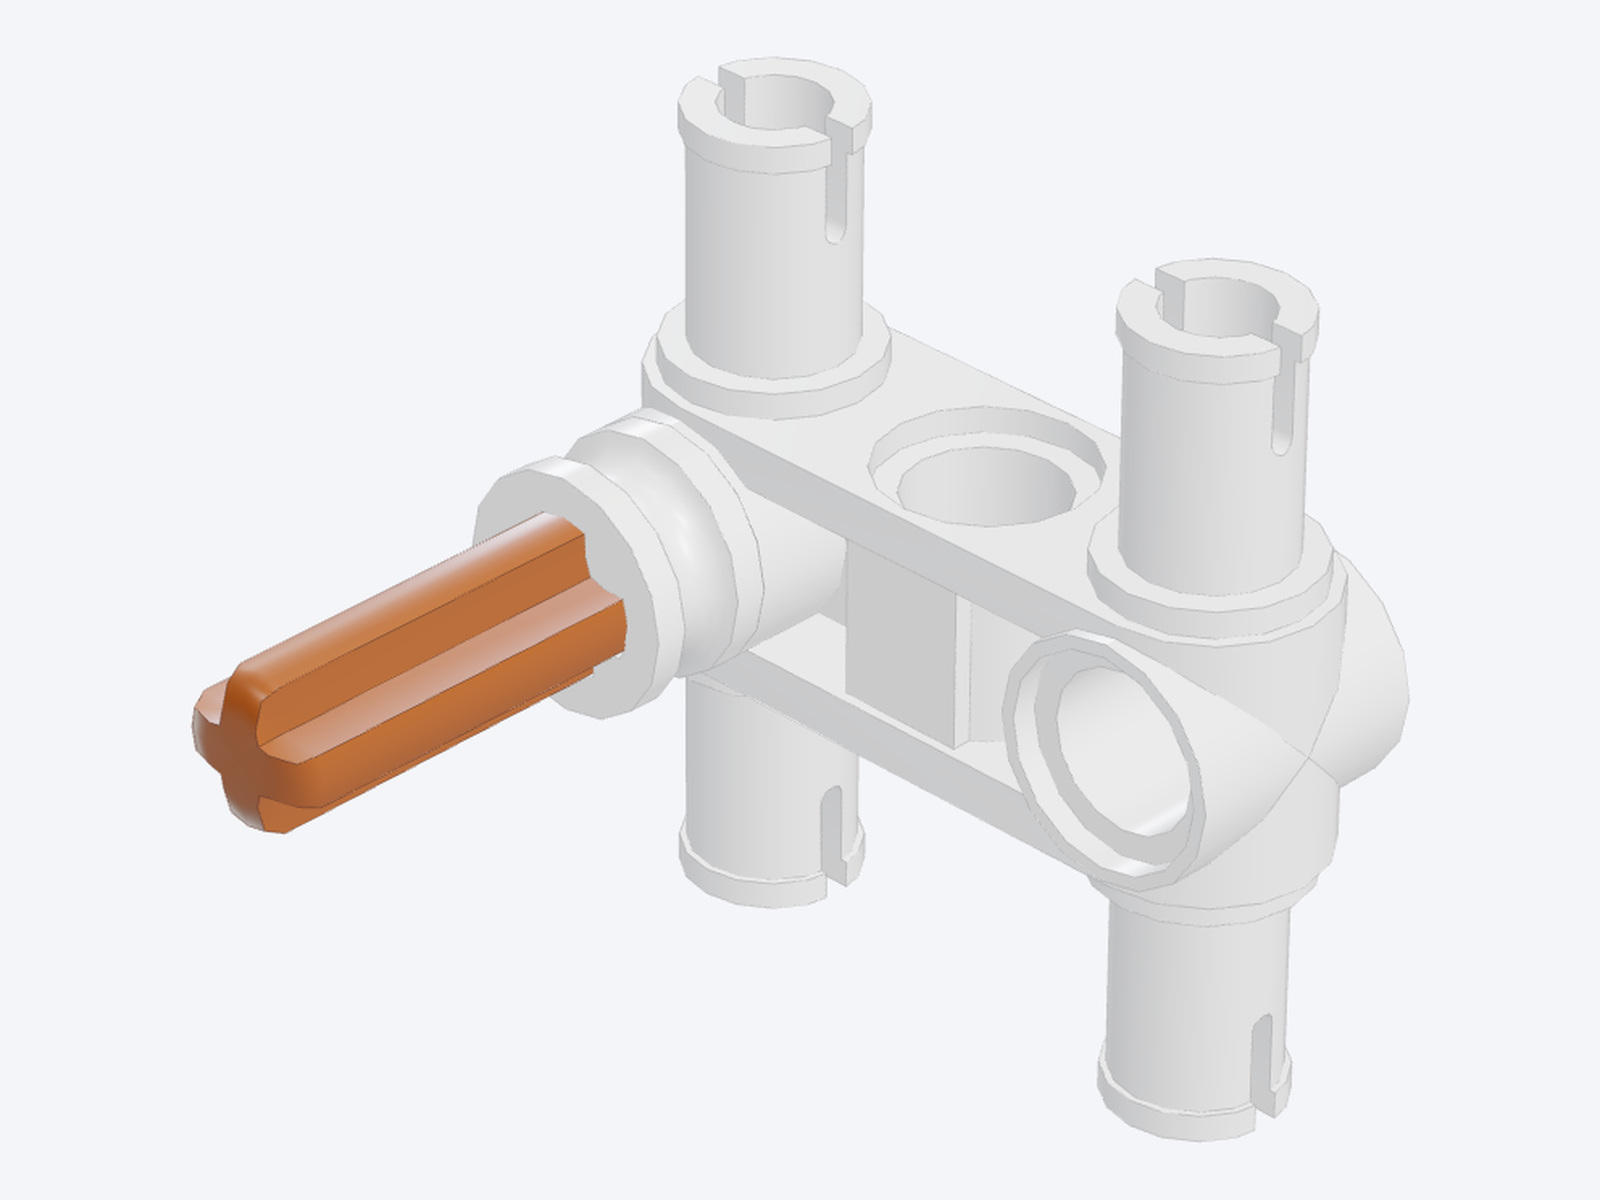
\includegraphics[width=.32\linewidth]{figures/ldraw/print/clean-sequence-1.jpg}
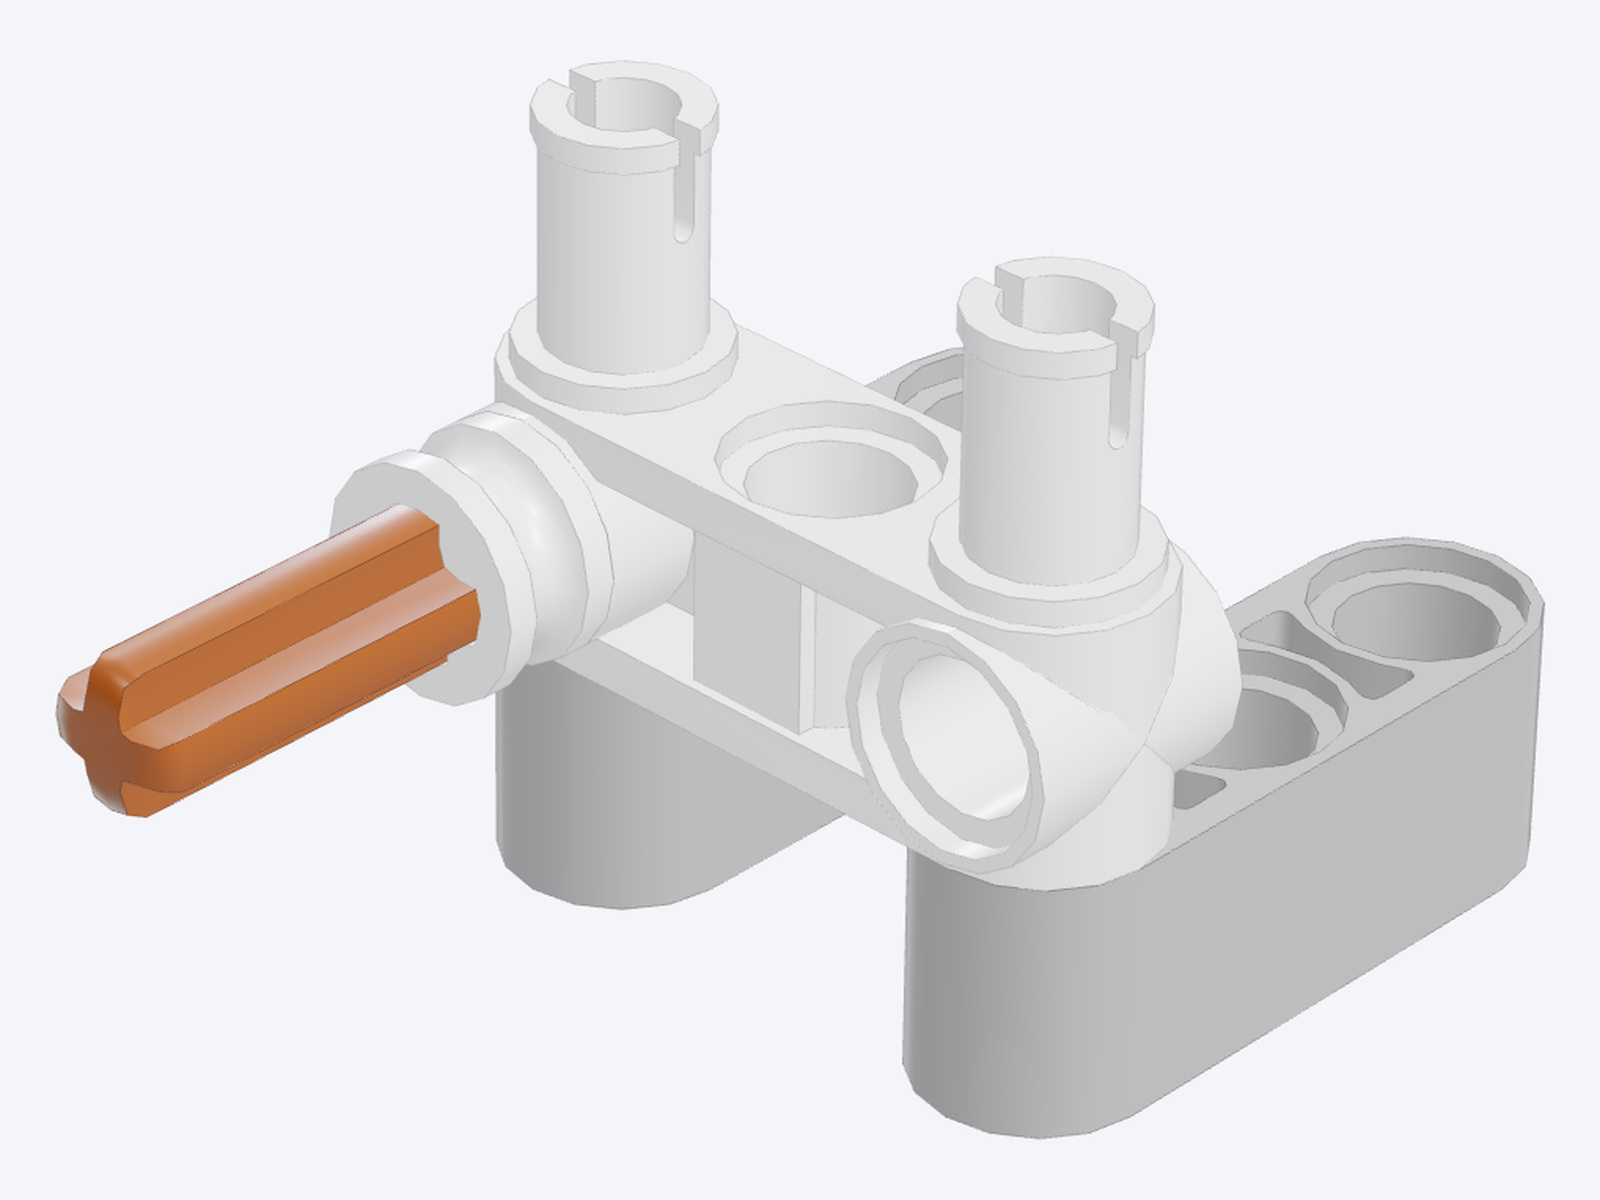
\includegraphics[width=.32\linewidth]{figures/ldraw/print/clean-sequence-2.jpg}
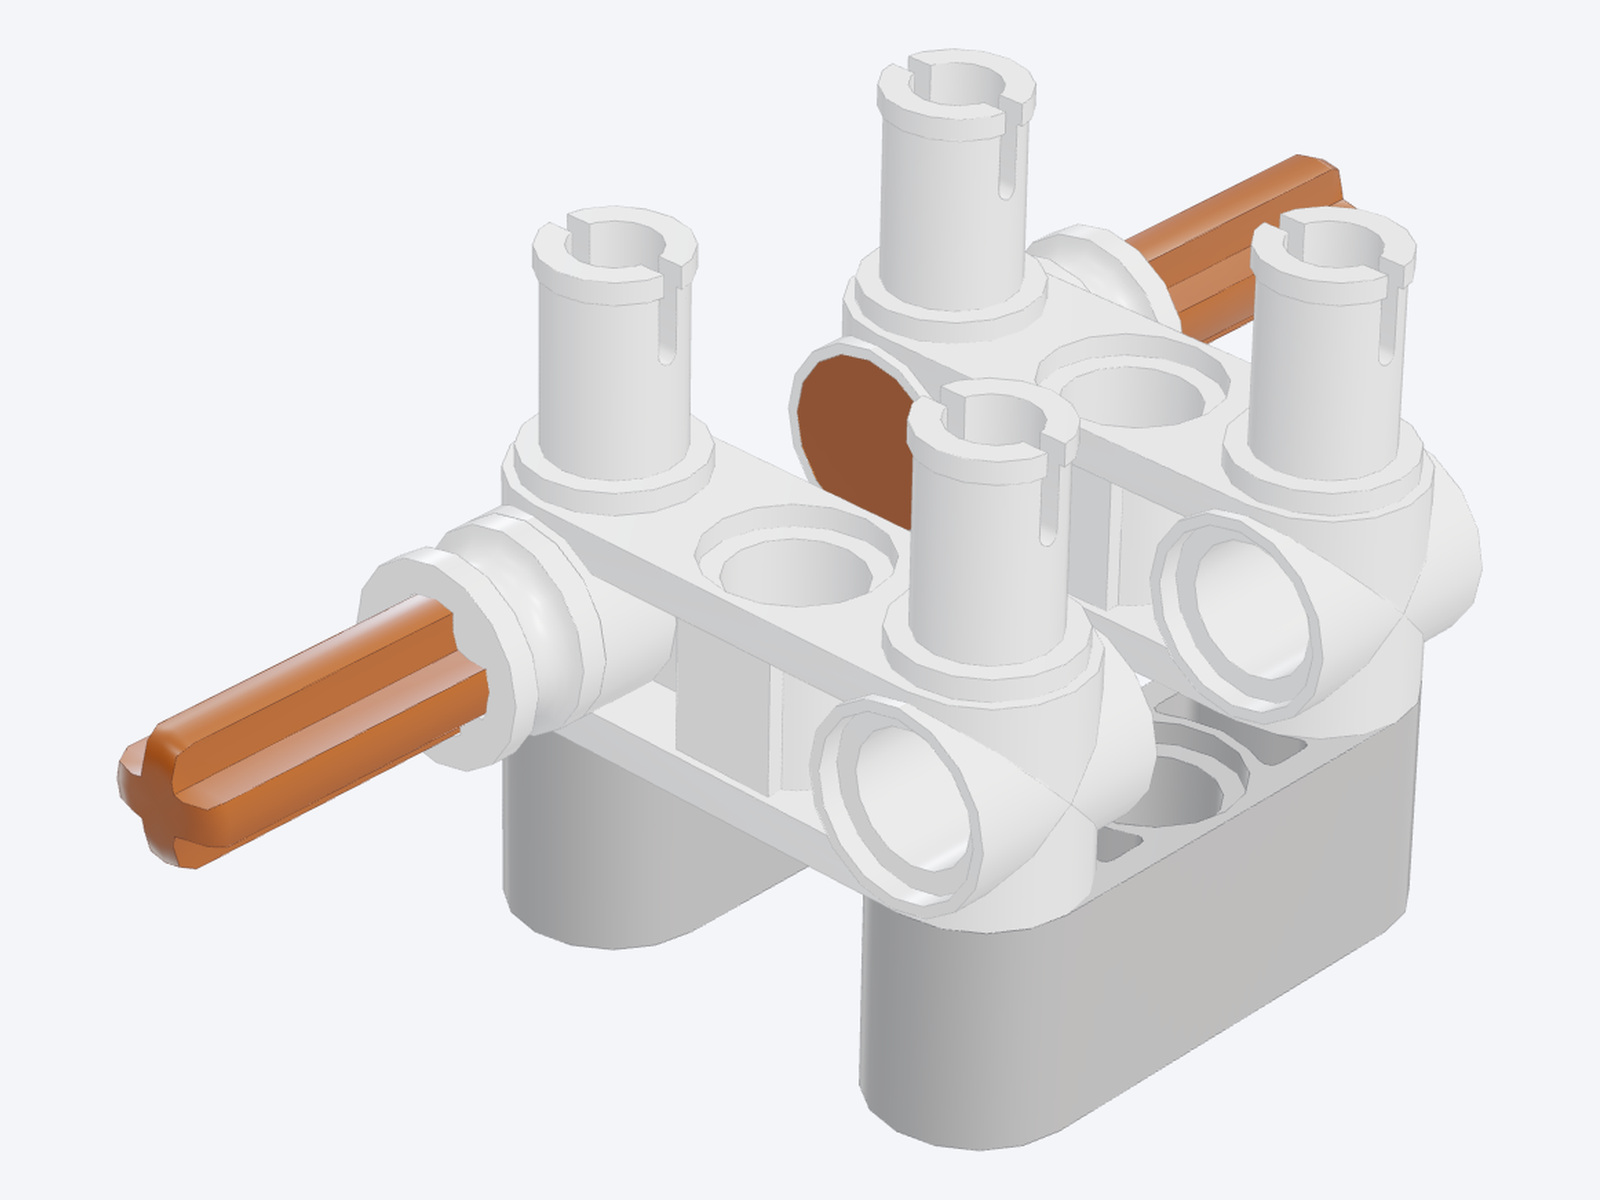
\includegraphics[width=.32\linewidth]{figures/ldraw/print/clean-sequence-3.jpg}\\
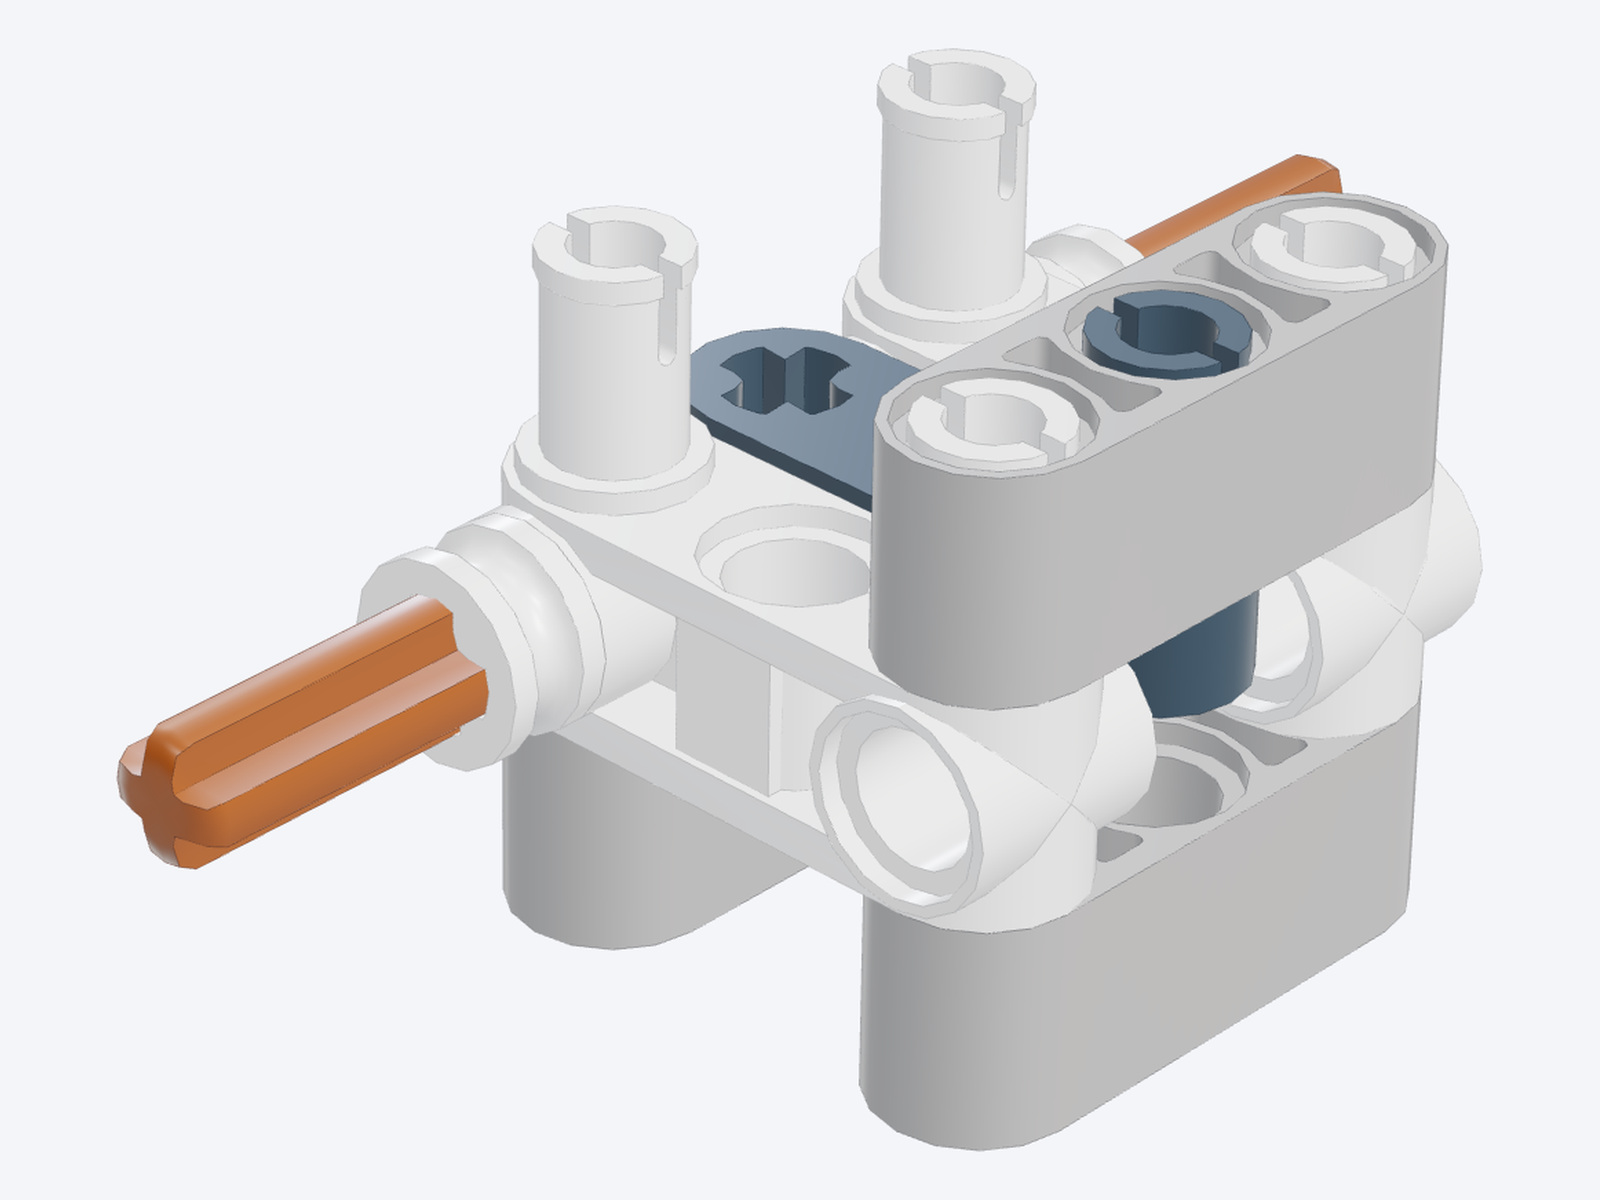
\includegraphics[width=.32\linewidth]{figures/ldraw/print/clean-sequence-4.jpg}
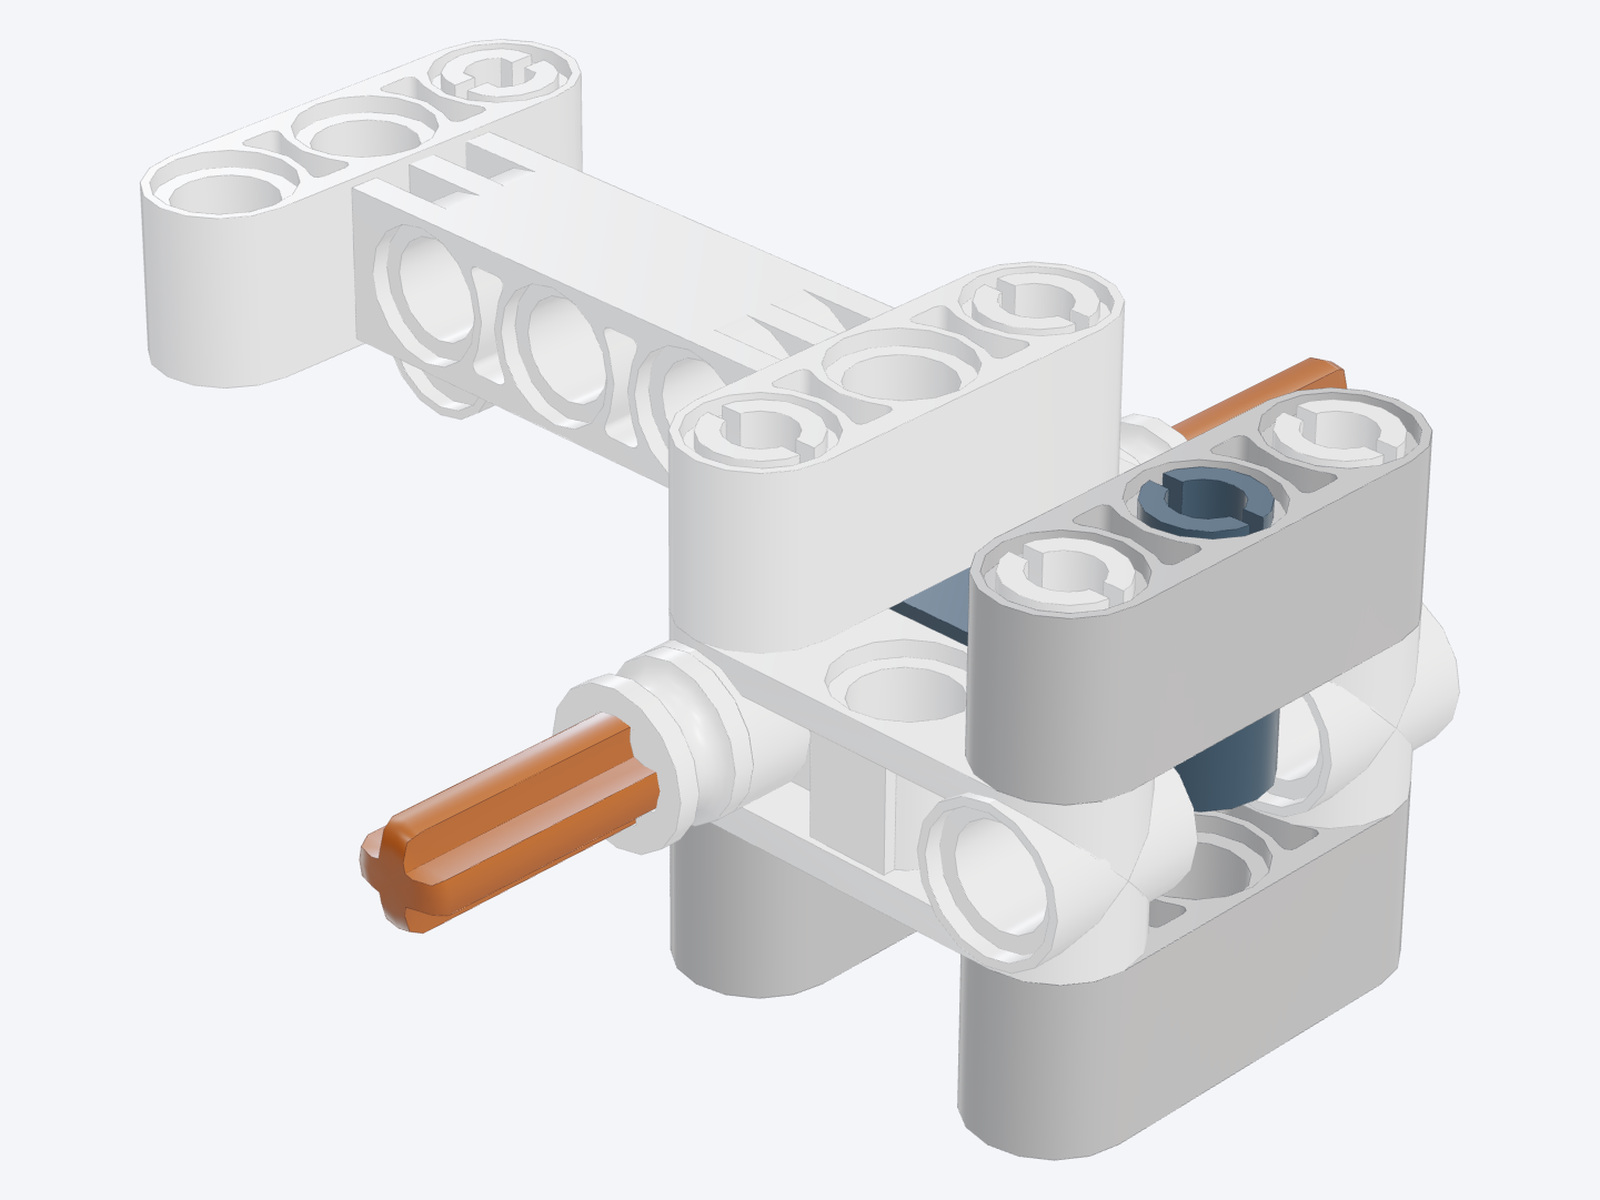
\includegraphics[width=.32\linewidth]{figures/ldraw/print/clean-sequence-5.jpg}
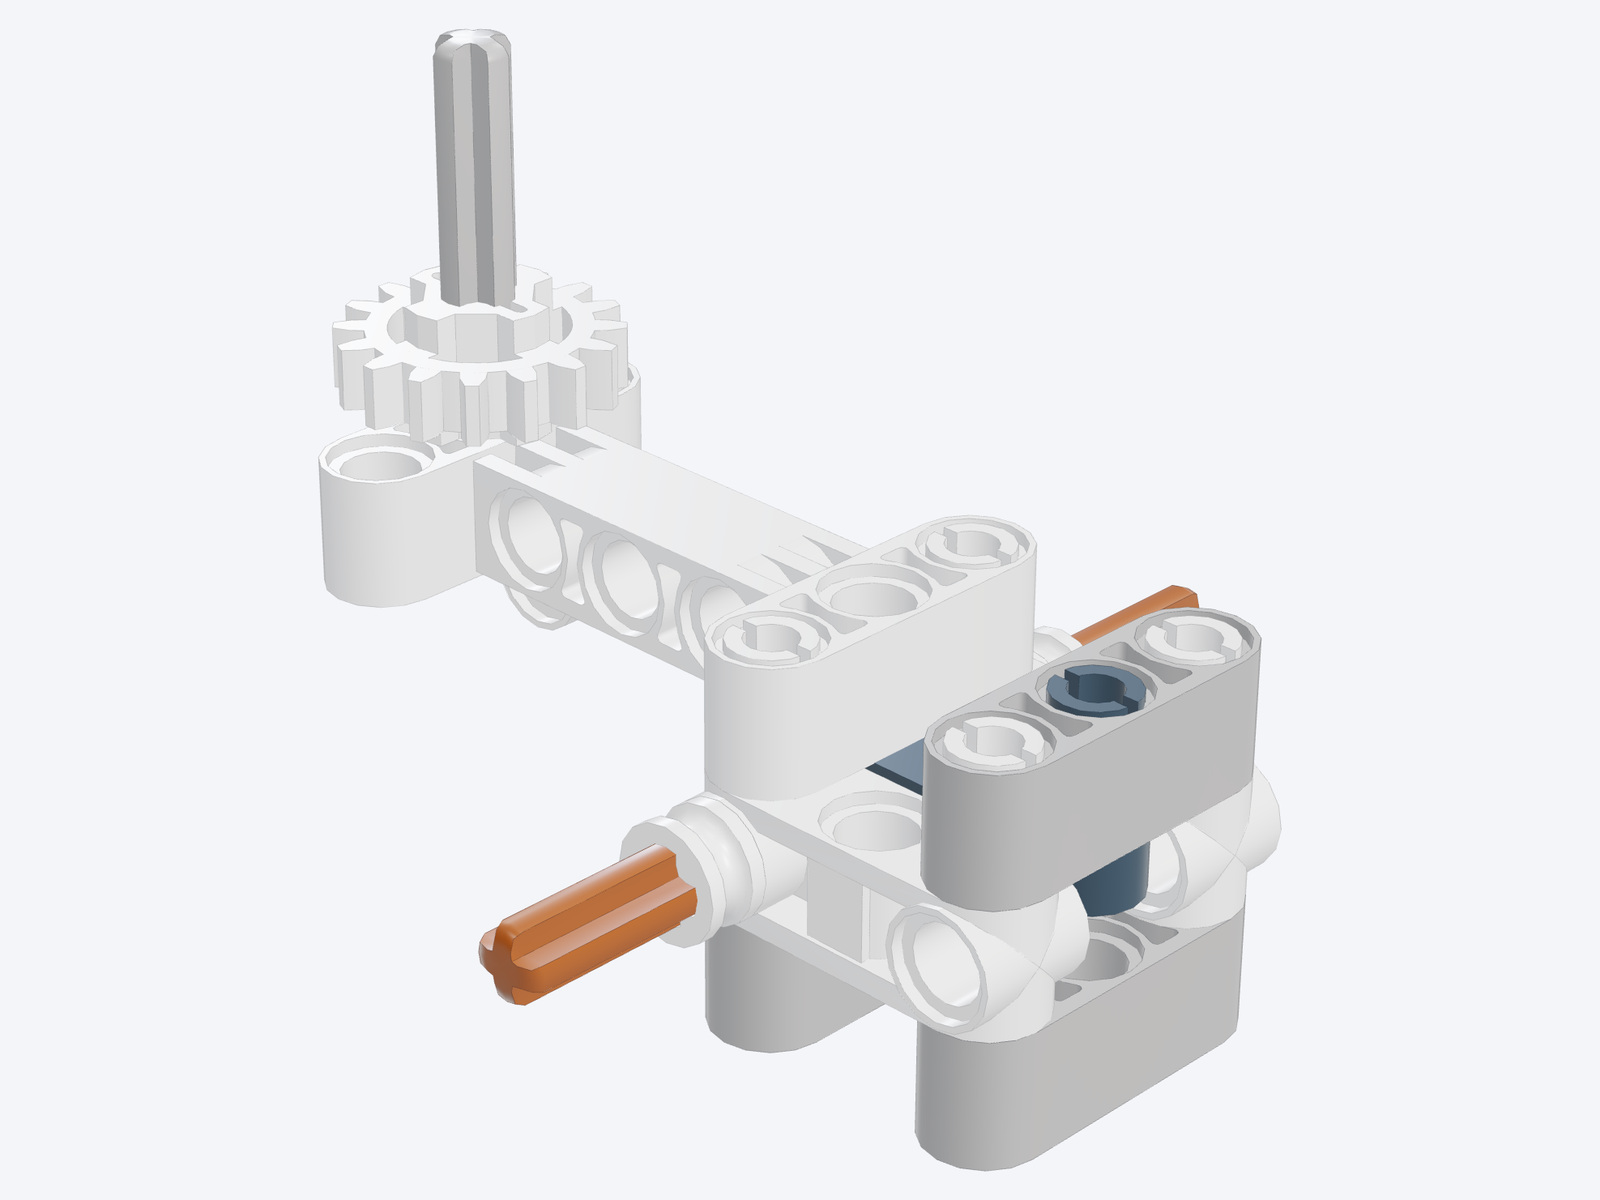
\includegraphics[width=.32\linewidth]{figures/ldraw/print/clean-sequence-6.jpg}
\end{center}
\begin{table}[h]
\centering
\caption{Executable six-action trace. The action budget is six and
the final goal is \texttt{done-6}. No insertion trajectory is specified.}
\begin{tabular}{rllrl}
\toprule
Step & Prerequisite & Added IDs & $|V|$ & New fact\\\midrule
1 & \texttt{start} & \texttt{B0001--B0003} & 3 & \texttt{done-1}\\
2 & \texttt{done-1} & \texttt{B0004--B0005} & 5 & \texttt{done-2}\\
3 & \texttt{done-2} & \texttt{B0006--B0008} & 8 & \texttt{done-3}\\
4 & \texttt{done-3} & \texttt{B0009--B0010} & 10 & \texttt{done-4}\\
5 & \texttt{done-4} & \texttt{B0011--B0012} & 12 & \texttt{done-5}\\
6 & \texttt{done-5} & \texttt{B0013--B0014} & 14 & \texttt{done-6}\\
\bottomrule
\end{tabular}

\end{table}

\begin{table}[h]
\centering\small
\caption{How the same source supports distinct question operations.
The sequence does not impose a six-level difficulty hierarchy.}
\begin{tabularx}{\linewidth}{lX}
\toprule
Family & Relation to the source and replay\\\midrule
Color / part type & Bind a numbered source instance and inspect its original appearance.\\
Distance & Compare provided geometry centers for numbered source candidates.\\
Interface / neighbors & Query recognized connector evidence for numbered parts.\\
Graph deletion & Delete a target from the supplied local graph; do not change the CAD source.\\
Step lookup & Find the expanded source step where a selected instance appears.\\
Step sequence & Execute the six given source-window steps in predecessor order.\\
Restoration & Restore a hidden source instance; this is independent of STEP ordering.\\
Evidence controls & State what coverage and geometric audits can establish.\\
\bottomrule
\end{tabularx}
\end{table}

\clearpage
\subsection{Accepted and Rejected Restoration}
The following panels show the same source with \texttt{B0094}
temporarily hidden, restored by its valid action, and still hidden
after an unknown action is rejected. Visible counts are 128, 129 and
128, respectively. The camera focuses the target's region and stays
fixed across the three states. No geometry is moved.
\begin{center}
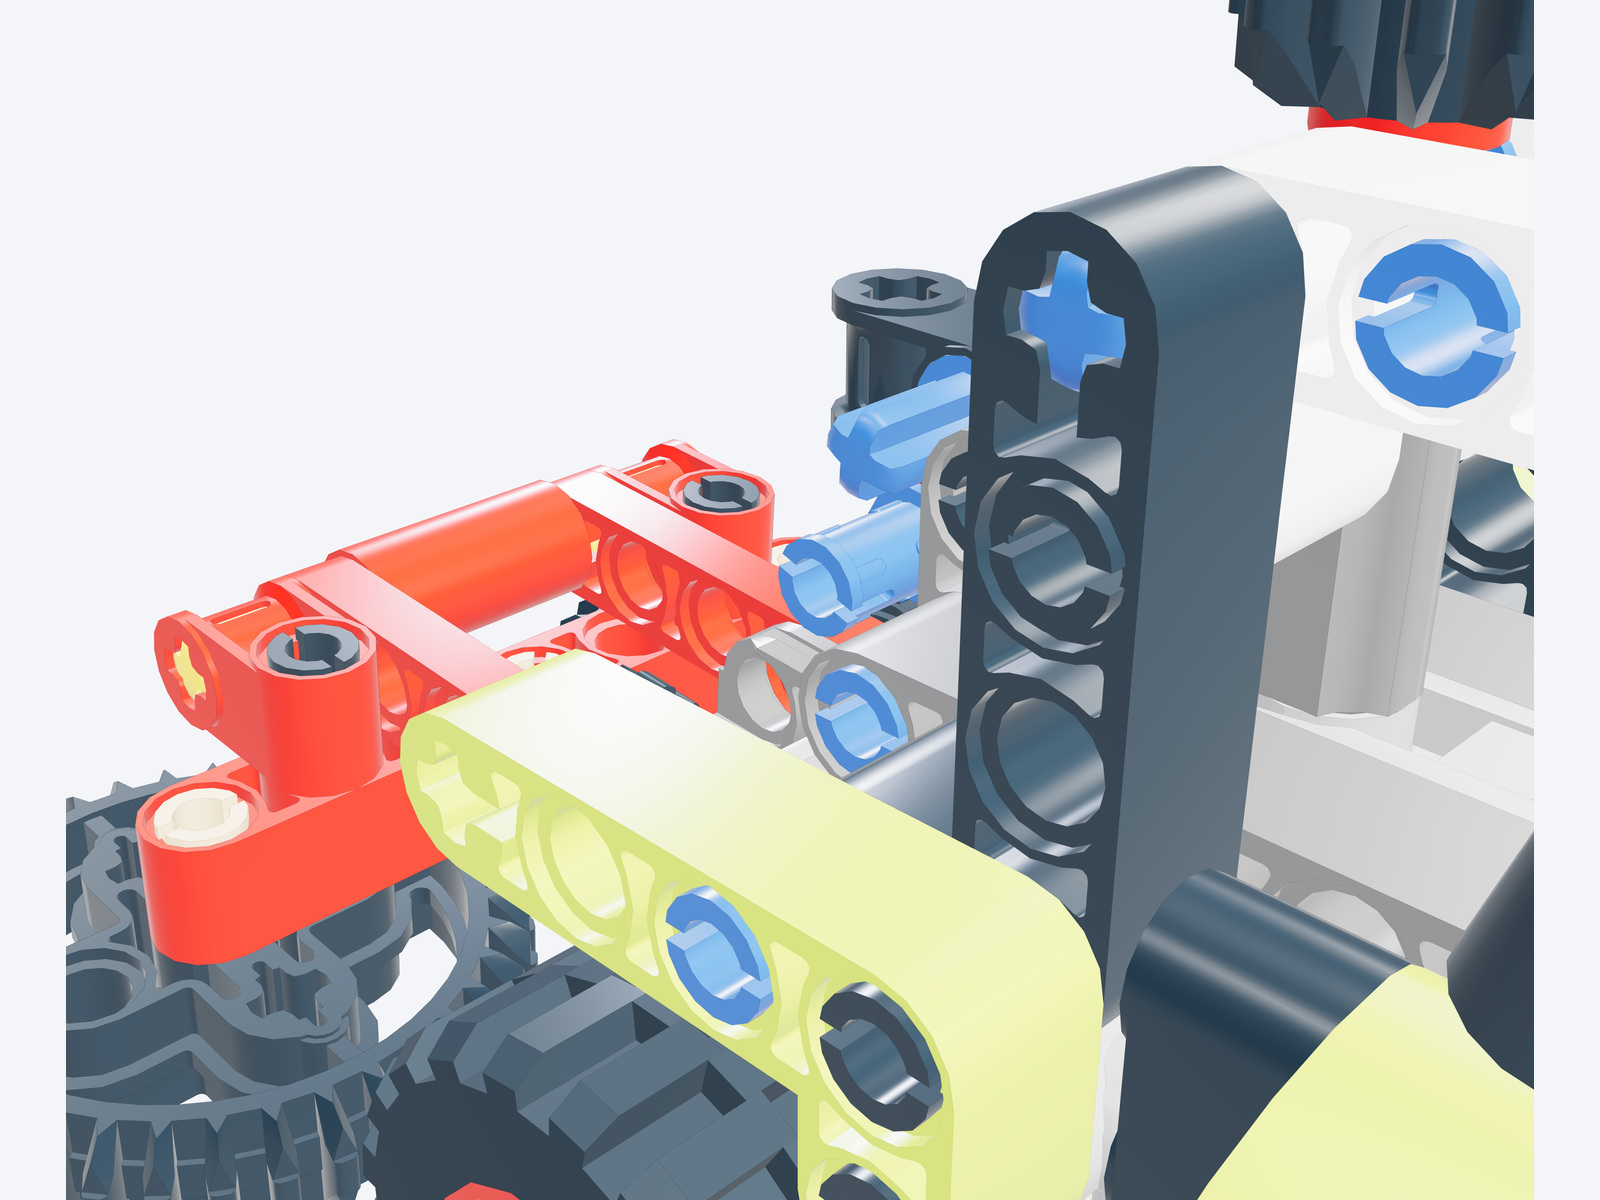
\includegraphics[width=.32\linewidth]{figures/ldraw/print/clean-restore-before.jpg}
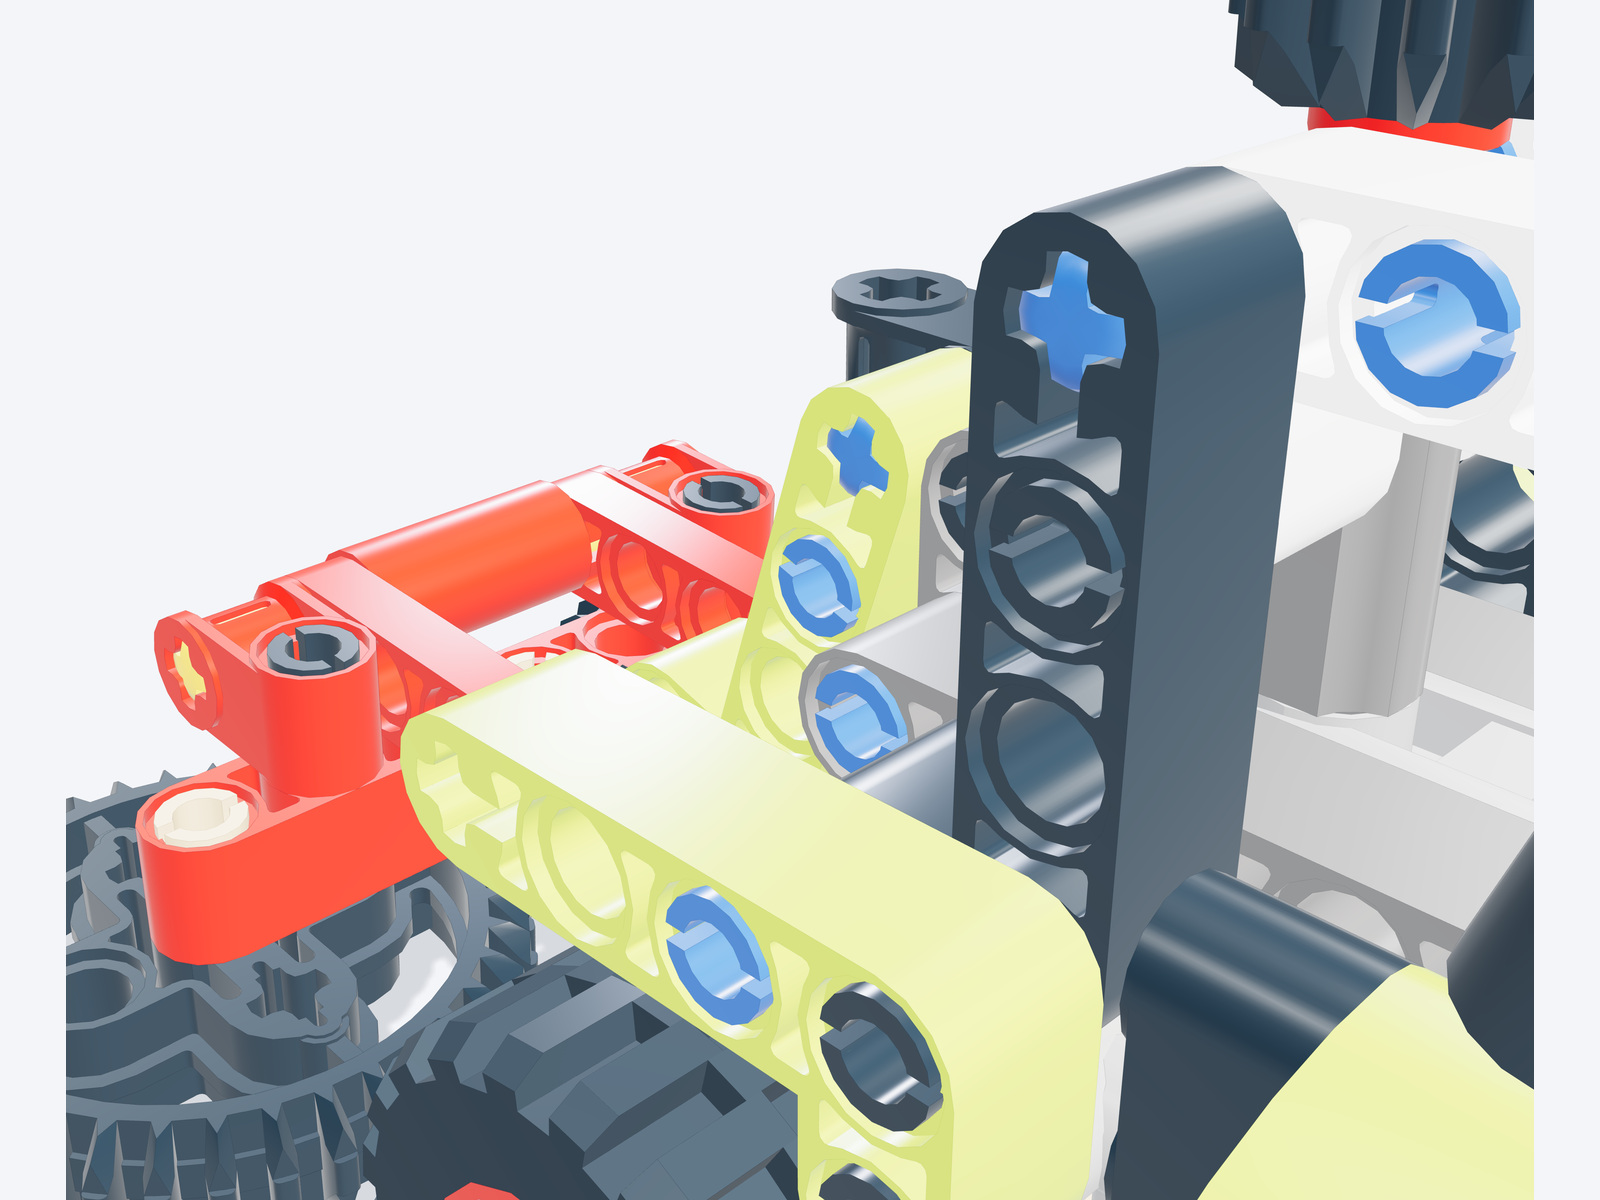
\includegraphics[width=.32\linewidth]{figures/ldraw/print/clean-restore-after.jpg}
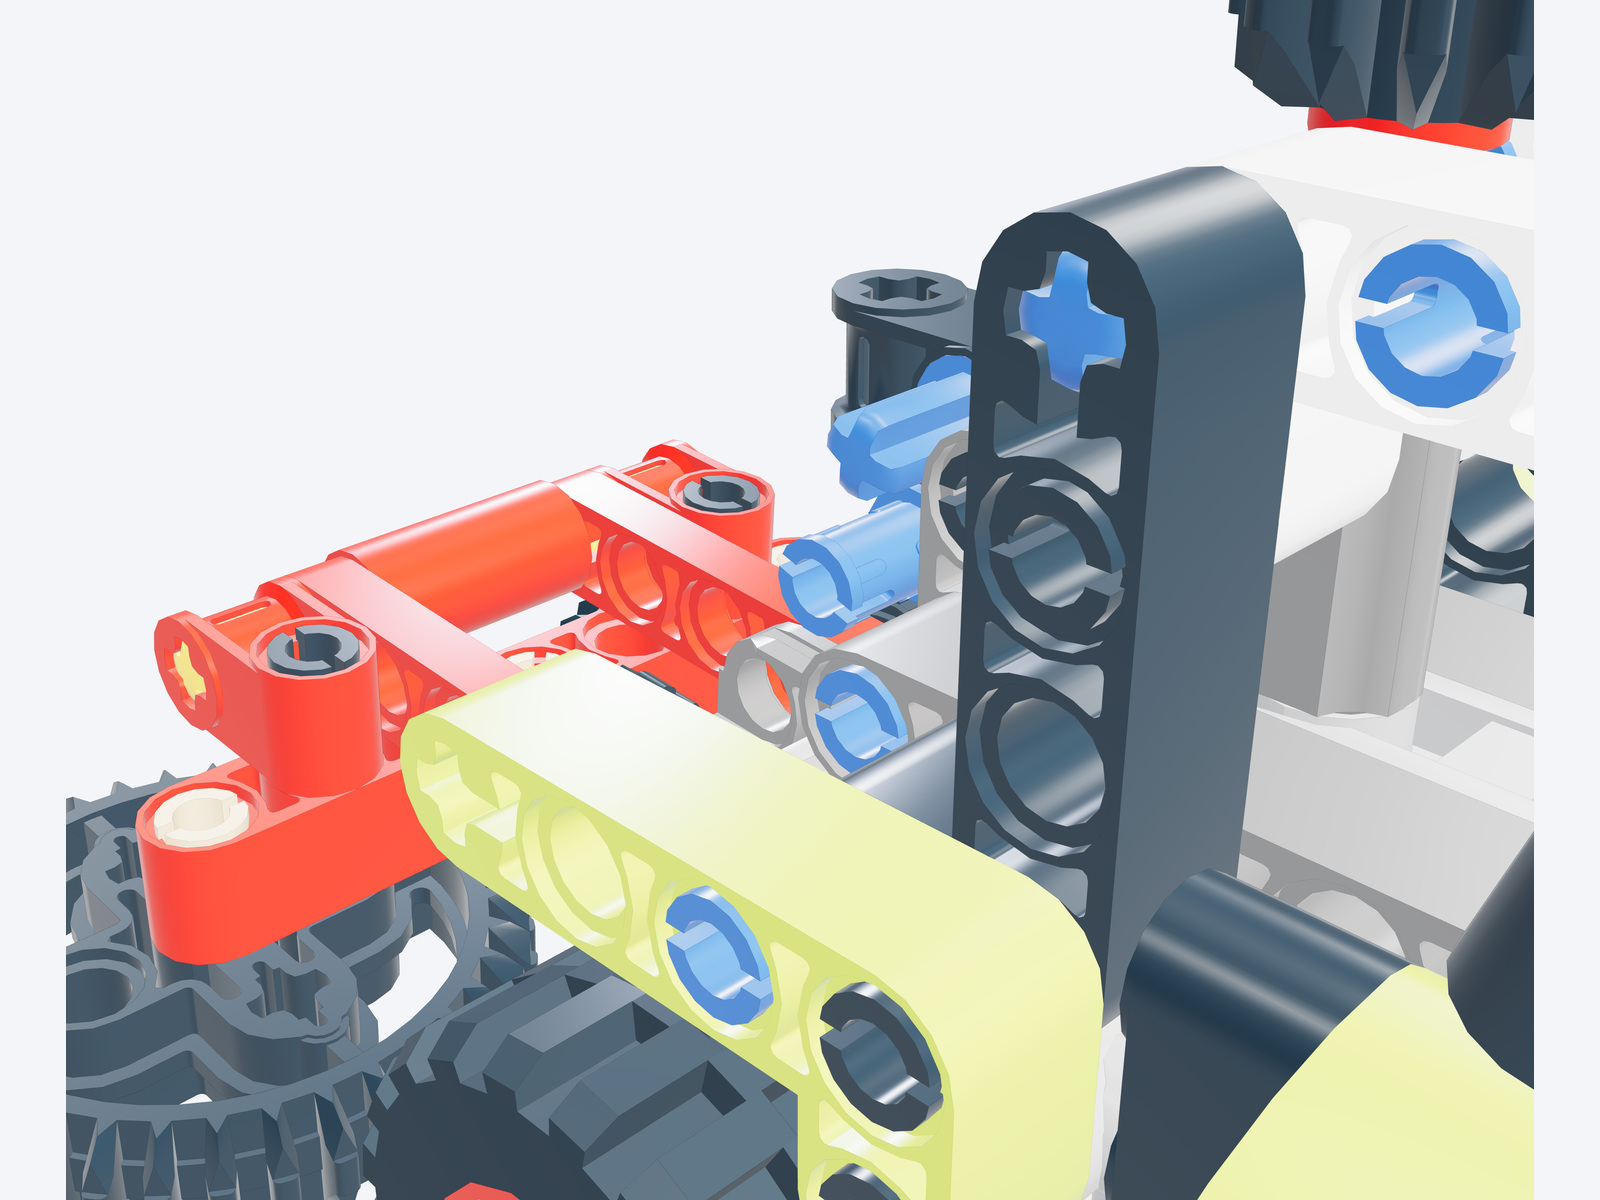
\includegraphics[width=.32\linewidth]{figures/ldraw/print/clean-restore-invalid.jpg}
\end{center}

\begin{table}[h]
\centering\small
\caption{Restoration transition contract for the worked target. Source
instance \texttt{brick\_000094} is displayed as \texttt{B0094}.}
\begin{tabularx}{\linewidth}{lX}
\toprule
Field & Value or rule\\\midrule
Target & \texttt{B0094}; all other source instances remain visible.\\
Accepted action & \texttt{restore-B0094}, requiring the target's missing fact.\\
Fact update & Delete missing-target; add present-target; preserve distractor presence.\\
Visibility update & Reveal the target at its original source transform.\\
Budget & One action of unit cost.\\
Rejected control & \texttt{unknown}; no matching public action, so no state update.\\
Success & Target present, distractor present, target missing fact absent.\\
Out of scope & A collision-free insertion, contact force or stability proof.\\
\bottomrule
\end{tabularx}
\end{table}

The file \path{publication-renders.json} records the new captures.
It includes task IDs, source hash, visibility snapshots and image checksums.
Earlier numbered checkpoints remain in \path{worked-renders.json}.
Original pixels are retained alongside all print derivatives.

\section{Evaluation Design and Missing-Result Convention}
Every blank numeric cell in the following tables means \emph{not run}.
The machine-readable \texttt{ldraw-experiments.json} stores these values
as null. Empty cells are neither zeros nor unavailable successful
results. There are no learned-model or human measurements to aggregate.
Candidate families are planning entries; exact checkpoint revisions,
API model identifiers, prompts, decoding and tools must be frozen
before execution.

\subsection{Run Configuration}
Each run record should include dataset and source hashes, model
identifier, prompt hash, decoding parameters, seed when supported,
input image dimensions, observation condition, tool permissions,
call budget, timeout, hardware or API backend, and timestamp.
Question-level receipts should retain response text, parsed output,
validity, exact success, failure category, tool calls, action trace,
latency, token counts and billed cost when available. Retries and
failures remain visible in these receipts.

The primary condition supplies each task's designated public input.
Static V tasks use the frozen numbered image. Interactive V adds
declared camera and isolation tools. S, G and E receive their public
structured evidence. Withholding evidence is an explicit ablation.
No model receives review answers or source color/type fields for V.

\subsection{Aggregation and Split Policy}
Micro accuracy weights tasks equally. Source-macro accuracy first
averages eligible tasks within each source, then averages sources with
at least one eligible task. Per-family and per-modality scores use the
same eligibility convention. Set F1 is secondary to exact neighbor-set
success. Action-format validity, legal execution and goal success are
reported separately.

Proposed 95\% intervals use 10,000 source-cluster bootstrap replicates
and a published seed. A paired comparison resamples the same sources
for both conditions. The source corpus has only 24 clusters, including
two D3 sources, so scale-specific uncertainty needs explicit caveats.
Repeated decoding should be reported within source rather than treated
as additional independent scenes.

Any training protocol must freeze grouped folds before fitting models.
All views, tasks, numbered permutations and alternative builds of a set
stay together. Inventory-neighbor inspection supplements the set-family
rule. This draft does not claim a finalized training split or
uncontaminated test set.

\clearpage
\section{Unrun Model and Diagnostic Tables}
\begin{table}[h]
\centering\small
\caption{Planned exact success (\%) by candidate family and input.
V: 140; S: 169; G: 233; E: 75. Micro and Macro follow the main protocol.}
\begin{tabular}{lrrrrrr}
\toprule
Candidate family & V & S & G & E & Micro & Macro\\\midrule
SmolVLM &  &  &  &  &  & \\
Qwen3-VL &  &  &  &  &  & \\
Llama 4 &  &  &  &  &  & \\
GPT-4.1 &  &  &  &  &  & \\
Gemini &  &  &  &  &  & \\
Claude &  &  &  &  &  & \\
\bottomrule
\end{tabular}

\end{table}

\begin{table}[h]
\centering\small
\caption{Planned per-family exact success (\%). Column abbreviations:
SmolVLM, Qwen3-VL, Llama 4, GPT-4.1, Gemini and Claude.
The $N$ column is measured dataset size; all score columns are empty.}
\begin{tabular}{llrrrrrr}
\toprule
Task family & N & Smol & Qwen & Llama & GPT & Gemini & Claude\\\midrule
Color & 73 &  &  &  &  &  & \\
Part type & 67 &  &  &  &  &  & \\
Distance & 73 &  &  &  &  &  & \\
Interface & 87 &  &  &  &  &  & \\
Neighbors & 73 &  &  &  &  &  & \\
Coverage & 17 &  &  &  &  &  & \\
Evidence limit & 24 &  &  &  &  &  & \\
Step lookup & 55 &  &  &  &  &  & \\
Step sequence & 17 &  &  &  &  &  & \\
Restoration & 58 &  &  &  &  &  & \\
Graph deletion & 73 &  &  &  &  &  & \\
\bottomrule
\end{tabular}

\end{table}

\begin{table}[h]
\centering\small
\caption{Planned source-scale exact success (\%) and overall source-macro
95\% confidence interval. Scale bands do not assert human difficulty.}
\begin{tabular}{lrrrrr}
\toprule
Candidate family & D1 & D2 & D3 & D4 & 95\% CI\\\midrule
SmolVLM &  &  &  &  & \\
Qwen3-VL &  &  &  &  & \\
Llama 4 &  &  &  &  & \\
GPT-4.1 &  &  &  &  & \\
Gemini &  &  &  &  & \\
Claude &  &  &  &  & \\
\bottomrule
\end{tabular}

\end{table}

\begin{table}[h]
\centering\small
\caption{Planned action-task evaluation on 75 tasks. Valid: well-formed
output; Goal: legal execution reaching the goal. Cost and Steps are
means over successful tasks, accompanied by the success denominator.}
\begin{tabular}{lrrrr}
\toprule
Candidate family & Valid \% & Goal \% & Cost & Steps\\\midrule
SmolVLM &  &  &  & \\
Qwen3-VL &  &  &  & \\
Llama 4 &  &  &  & \\
GPT-4.1 &  &  &  & \\
Gemini &  &  &  & \\
Claude &  &  &  & \\
\bottomrule
\end{tabular}

\end{table}

\clearpage
\subsection{Information and Tool Ablations}
Hold the model, prompts outside the changed condition and eligible
questions fixed. Static, camera-control and isolation conditions use
the same 140 visual items. A text-without-image control retains the
prompt, numbered candidates and options; it tests priors without
visual evidence. Graph withholding removes supplied edges for the
233 graph items and is not comparable to the primary contract without
explicit qualification.

\begin{table}[h]
\centering\small
\caption{Unrun ablations. Acc.\ and Valid are percentages; Calls is
mean tool calls across eligible tasks. The public solver's separately
verified goal success does not fill unmeasured resource-log cells.}
\begin{tabularx}{\linewidth}{Xlrrr}
\toprule
Condition & N & Acc. & Valid & Calls\\\midrule
Static numbered image & 140 &  &  & \\
+ rotate / zoom & 140 &  &  & \\
+ ID isolation & 140 &  &  & \\
Text without image & 140 &  &  & \\
Structured public input & 477 &  &  & \\
Graph edges withheld & 233 &  &  & \\
Public action solver & 75 &  &  & \\
\bottomrule
\end{tabularx}

\end{table}

\subsection{Paired Robustness}
An ID permutation is a bijection applied consistently to public
references, visible labels, graph endpoints, action names and scorer
mapping. Choice permutations preserve semantic answers. Camera
perturbations preserve the source geometry and task identity, while
color nuisance applies only to the 67 type-correspondence tasks that
explicitly ignore color. Evaluation copies do not overwrite source
files. Equivalent edge ordering preserves the same simple graph.

\begin{table}[h]
\centering\small
\caption{Unrun paired robustness. Base and Changed are exact success
(\%); Consist.\ is mapped-output agreement (\%). Agreement alone can
include two wrong answers, so correct paired agreement must also be
retained in run receipts. Pool sizes are known; scores are unmeasured.}
\begin{tabular}{llrrr}
\toprule
Perturbation & Eligible & Base & Changed & Consist.\\\midrule
ID permutation & 617 &  &  & \\
Choice-order permutation & 542 &  &  & \\
Camera perturbation & V: 140 &  &  & \\
Color nuisance & Type: 67 &  &  & \\
Equivalent edge ordering & G: 233 &  &  & \\
\bottomrule
\end{tabular}

\end{table}

\subsection{Efficiency}
Token counts should include input and output separately in receipts.
Calls include unsuccessful tool/API calls; latency is end-to-end
per task including allowed retries. The p50 and p95 summarize the same
eligible pool. Report model-loading costs separately for local models.
USD denotes actual billed inference cost; local energy or hardware cost
requires a separately declared accounting rule.

\begin{table}[h]
\centering\small
\caption{Unrun resource measurements. Tokens, Calls and USD are means
per eligible task; latency quantiles are seconds. Unbilled or untracked
quantities must not be filled with an assumed zero.}
\input{ldraw-plan-resources.tex}
\end{table}

\clearpage
\section{Human and Physical Validation Plan}
\subsection{Human Review}
The proposed procedure uses two independent reviewers per sampled
item, with source-stratified coverage and adjudication of disagreements.
Report the sampling rule, reviewed denominator, pass criteria, raw
agreement and an appropriate chance-adjusted statistic. A pass must
distinguish readable grounding from correct semantics. Ambiguous
visual equivalence, occluded leader lines, faulty distractors and
unsupported physical language receive separate reason codes.

The review application stores source hash, task ID, numbered operands,
pass/fail, reason and timestamp. Failure requires a written explanation.
Export and import support batch correction without changing historical
feedback. No automated contract check is counted as human acceptance.

\begin{table}[h]
\centering\small
\caption{Unrun human assessment. Pool sizes are known.
Reviewed is a count; Pass and Agree are percentages over declared
denominators; Time is median seconds per reviewed unit.}
\begin{tabular}{llrrrr}
\toprule
Review stratum & Pool & Reviewed & Pass & Agree & Time\\\midrule
Visual grounding & 140 &  &  &  & \\
Structured questions & 477 &  &  &  & \\
All original sources & 24 &  &  &  & \\
Intersection candidates & 573 &  &  &  & \\
\bottomrule
\end{tabular}

\end{table}

\subsection{Physical Evidence}
Connector-aware inspection should categorize each intersection
candidate as intended mating, a mesh approximation issue, a source
problem or unresolved. The procedure must retain inspected pair IDs,
part definitions and evidence images. Unsupported connector parts need
their own denominator and adjudication. A rejected candidate may
require source exclusion or revised evidence; silently moving a source
part is not an admissible correction.

Insertion/extraction studies require start and goal configurations,
collision geometry and allowed neighboring motion. Dynamics studies
add mass, friction, contact, material and boundary conditions.
Physical assembly tests must specify parts, loads and measurement
procedures. These extensions are not already benchmark ground truth.

\begin{table}[h]
\centering\small
\caption{Unrun physical validation. Each row requires a declared unit
(pair, part, operation or assembly), sampling policy and acceptance
criterion. Counts cannot be pooled across procedures.}
\begin{tabular}{lrrrr}
\toprule
Validation procedure & Reviewed & Pass & Fail & Unresolved\\\midrule
Connector-aware pair inspection &  &  &  & \\
Unsupported-part adjudication &  &  &  & \\
Insertion / extraction study &  &  &  & \\
Gravity / friction simulation &  &  &  & \\
Physical assembly validation &  &  &  & \\
\bottomrule
\end{tabular}

\end{table}

\section{Reproduction and Audit Trail}
The release generator and independent source verifier bind questions
to unchanged MPD files and dependency locks. The publication generator
derives statistics, CSV tables and four vector Matplotlib plots from
the same bundles. It records input and output hashes. Descriptive
plots show measured source properties and choice priors; no performance
curve is inferred from an empty experimental cell.

Build commands and exact Python requirements accompany the manuscript.
PDF checks reject CJK text, unresolved references, overfull boxes,
out-of-page words, untracked raster images and captions inside brick
figure environments. Main content remains within the eight-page CVPR
budget. The source package includes the manuscript, figures, numerical
plot data and null-valued experiment specification.

The following dossiers summarize repeated connector pairs as unique
undirected edges for readability, matching graph-question semantics.
Full raw records, source-step provenance and action fact lists remain
in the versioned JSON. These human-readable summaries do not alter
task inputs or reference outputs.

\clearpage
\section{31028: Sea Plane}
53 source instances; 15 tasks; D1 scale band.

\par\noindent Perspective, front, side and top views follow in reading order. Original source transforms are preserved.
\begin{center}
\includegraphics[width=.48\linewidth]{figures/ldraw/print/31028-iso.jpg}
\includegraphics[width=.48\linewidth]{figures/ldraw/print/31028-front.jpg}\\
\includegraphics[width=.48\linewidth]{figures/ldraw/print/31028-side.jpg}
\includegraphics[width=.48\linewidth]{figures/ldraw/print/31028-top.jpg}\end{center}
\paragraph{Attribution.}Merlijn Wissink [legolijntje]. CC BY 2.0.\par\noindent\url{https://library.ldraw.org/omr/sets/259}
\paragraph{Source lock.}\small\texttt{d2619a85e973430a1b256d607fe8e44a}\\\texttt{865beb05ef63ac8028a5109c228ee97c}\normalsize
\paragraph{Evidence coverage.}Connector definitions cover 100.00\% of instances. The audit reports 1 recognized-graph components and 0 intersection candidates without a recognized mating pair. 0 instances have no connector definition. These counts do not certify physical defects or gravitational stability.
\paragraph{Instructions.}No author STEP replay or source-order question is provided.
\clearpage\subsection{Numbered visual input and complete question index}
Only relevant numbers are shown. The website can isolate any instance; public visual tasks provide their own numbered images. The following entries give every English prompt, all choice options, compact public evidence and the reference output. Raw repeated connector records and full action fact sets remain in the versioned JSON.
\begin{center}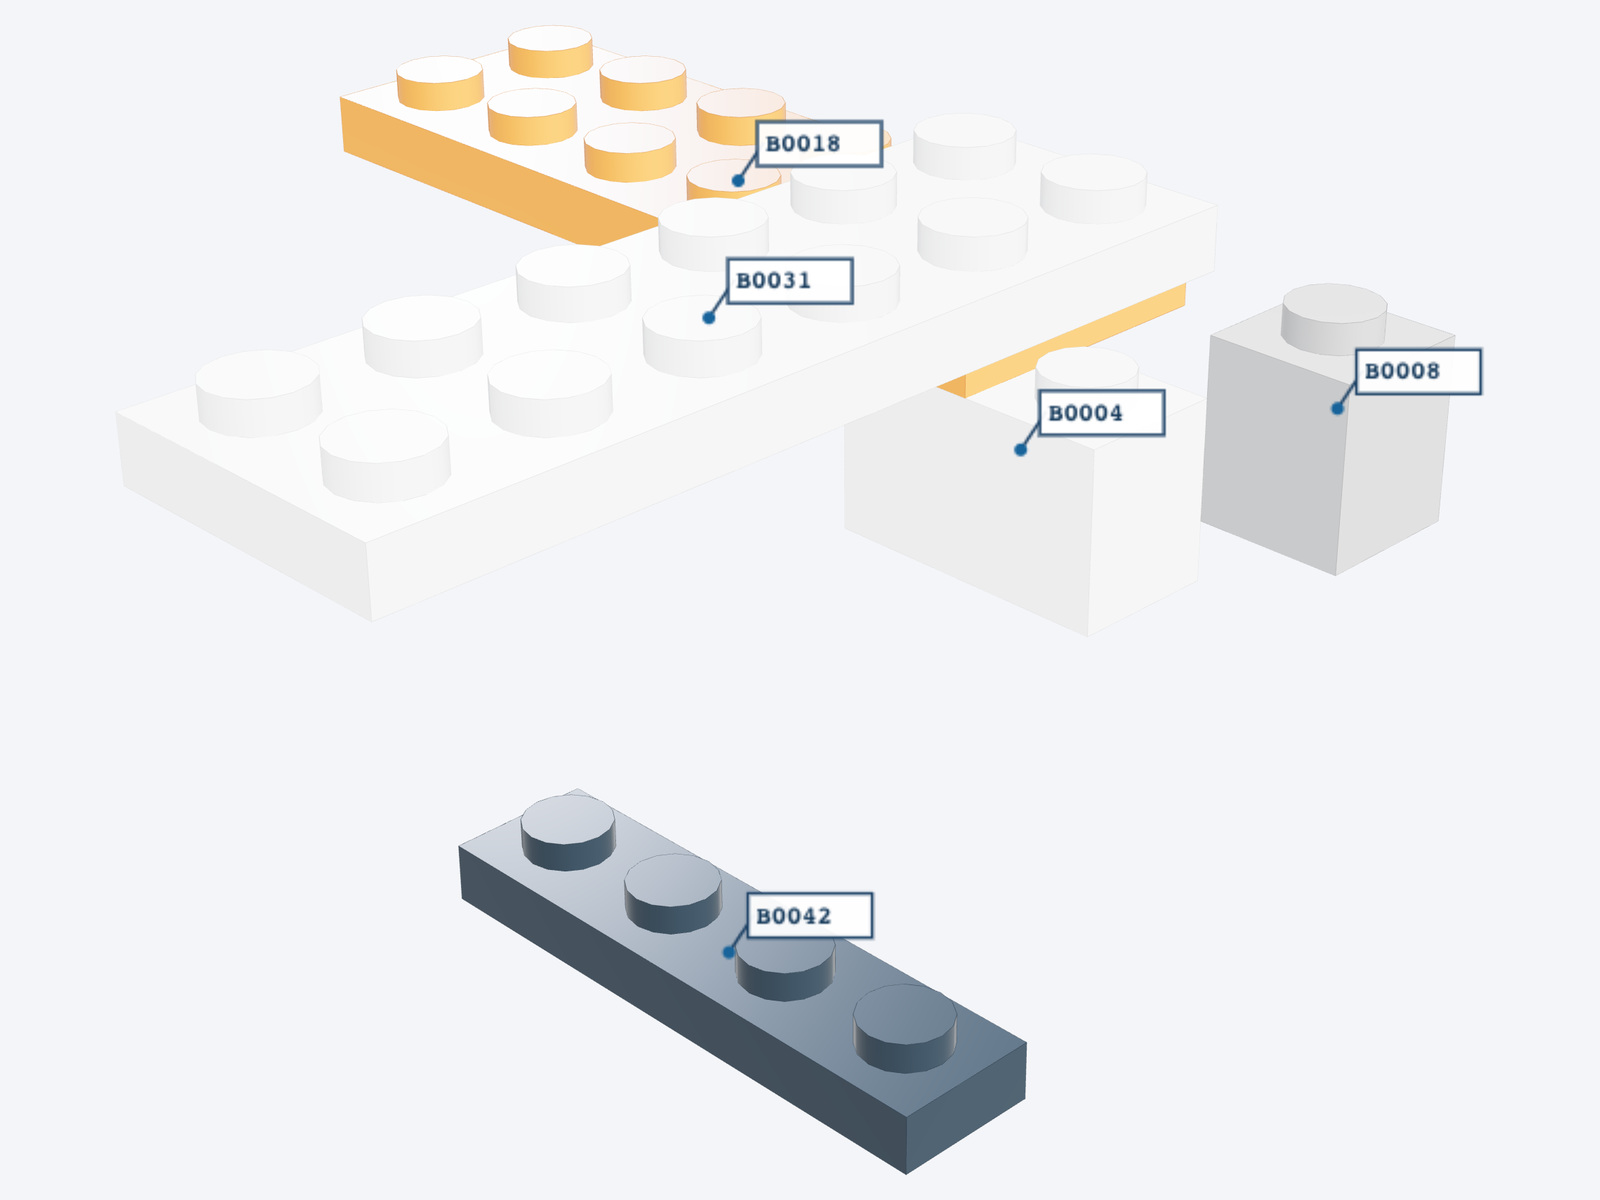
\includegraphics[width=.55\linewidth]{figures/ldraw/print/31028-numbered.jpg}\end{center}
\begin{enumerate}
\item \textbf{color-1}. Identify the original color of B0018; numbered isolation is allowed.\par {\small \textit{Input:} Numbered visual input; source attributes are withheld from the model. \par\textit{Options:} A: Black; B: Orange; C: Light Bluish Grey; D: Trans Brown. \par\textit{Reference output:} B.}
\item \textbf{shape-match-1}. Ignoring color and pose, which numbered instance has the same LDraw part type as B0018?\par {\small \textit{Input:} Numbered visual input; source attributes are withheld from the model. \par\textit{Options:} A: B0042; B: B0008; C: B0004; D: B0031. \par\textit{Reference output:} D.}
\item \textbf{distance-1}. Using the supplied geometry bounding-box centers, which candidate is nearest to B0018?\par {\small \textit{Input:} Centers (mm): B0018 = (0, 8.8, -36); B0028 = (0, 15.2, -24); B0043 = (-17.2, -12, 0); B0024 = (-20, 15.2, -56). \par\textit{Options:} A: B0043; B: B0028; C: B0024. \par\textit{Reference output:} B.}
\item \textbf{color-2}. Identify the original color of B0035; numbered isolation is allowed.\par {\small \textit{Input:} Numbered visual input; source attributes are withheld from the model. \par\textit{Options:} A: Black; B: Trans Orange; C: White; D: Trans Brown. \par\textit{Reference output:} D.}
\item \textbf{shape-match-2}. Ignoring color and pose, which numbered instance has the same LDraw part type as B0035?\par {\small \textit{Input:} Numbered visual input; source attributes are withheld from the model. \par\textit{Options:} A: B0045; B: B0038; C: B0034; D: B0012. \par\textit{Reference output:} C.}
\item \textbf{distance-2}. Using the supplied geometry bounding-box centers, which candidate is nearest to B0035?\par {\small \textit{Input:} Centers (mm): B0035 = (4, 15.92, 0); B0014 = (-12, 0.8, 8); B0006 = (0, -0.8, 0); B0027 = (-24, 12, -23.8). \par\textit{Options:} A: B0027; B: B0006; C: B0014. \par\textit{Reference output:} B.}
\item \textbf{interface-1}. Classify the supplied connector record for B0053 and B0006. This does not certify load capacity.\par {\small \textit{Input:} Record: family = axle; connector indices = 0, 1. \par\textit{Options:} A: fixed; B: axle; C: hinge; D: ball. \par\textit{Reference output:} B.}
\item \textbf{interface-2}. Classify the supplied connector record for B0042 and B0044. This does not certify load capacity.\par {\small \textit{Input:} Record: family = stud; connector indices = 11, 10. \par\textit{Options:} A: axle; B: fixed; C: stud; D: ball; E: hinge. \par\textit{Reference output:} C.}
\item \textbf{neighbors-1}. Select every candidate directly adjacent to B0027 in the supplied connector graph.\par {\small \textit{Input:} Unique undirected pairs: B0018 / B0027; B0027 / B0028; B0027 / B0031; B0031 / B0038. \par\textit{Options:} A: B0038; B: B0018; C: B0028; D: B0031; E: B0047. \par\textit{Reference output:} B, C, D.}
\item \textbf{graph-removal-1}. Delete B0027 and its incident edges from this local graph. How many connected components remain? Do not infer physical extractability.\par {\small \textit{Input:} Nodes: B0027, B0031, B0028, B0018, B0047, B0038. Unique undirected pairs: B0018 / B0027; B0027 / B0028; B0027 / B0031; B0031 / B0038. \par\textit{Options:} A: 6; B: 3; C: 4; D: 5. \par\textit{Reference output:} C.}
\item \textbf{neighbors-2}. Select every candidate directly adjacent to B0047 in the supplied connector graph.\par {\small \textit{Input:} Unique undirected pairs: B0044 / B0048; B0047 / B0048; B0047 / B0049; B0047 / B0050; B0049 / B0050. \par\textit{Options:} A: B0001; B: B0050; C: B0049; D: B0048; E: B0044. \par\textit{Reference output:} B, C, D.}
\item \textbf{graph-removal-2}. Delete B0047 and its incident edges from this local graph. How many connected components remain? Do not infer physical extractability.\par {\small \textit{Input:} Nodes: B0047, B0050, B0049, B0048, B0001, B0044. Unique undirected pairs: B0044 / B0048; B0047 / B0048; B0047 / B0049; B0047 / B0050; B0049 / B0050. \par\textit{Options:} A: 2; B: 5; C: 3; D: 4. \par\textit{Reference output:} C.}
\item \textbf{evidence-limit-1}. Only source geometry, connector matching and mesh intersection audits are available. Without mass, friction, material or dynamic tests, is gravitational stability established?\par {\small \textit{Input:} Available evidence: Original CAD; Connector inference; Inset-mesh intersection candidates. \par\textit{Options:} A: Not established by this evidence; B: Established. \par\textit{Reference output:} A.}
\item \textbf{restore-instance-1}. The display copy hides B0018. Restore only that numbered instance, preserving all other instances and source poses.\par {\small \textit{Input:} Target: B0018. Action budget: 1. All other instances initially remain visible. \par\textit{Reference output:} restore-B0018.}
\item \textbf{restore-instance-2}. The display copy hides B0035. Restore only that numbered instance, preserving all other instances and source poses.\par {\small \textit{Input:} Target: B0035. Action budget: 1. All other instances initially remain visible. \par\textit{Reference output:} restore-B0035.}
\end{enumerate}
\clearpage
\section{31027: Blue Racer}
67 source instances; 17 tasks; D1 scale band.

\par\noindent Perspective, front, side and top views follow in reading order. Original source transforms are preserved.
\begin{center}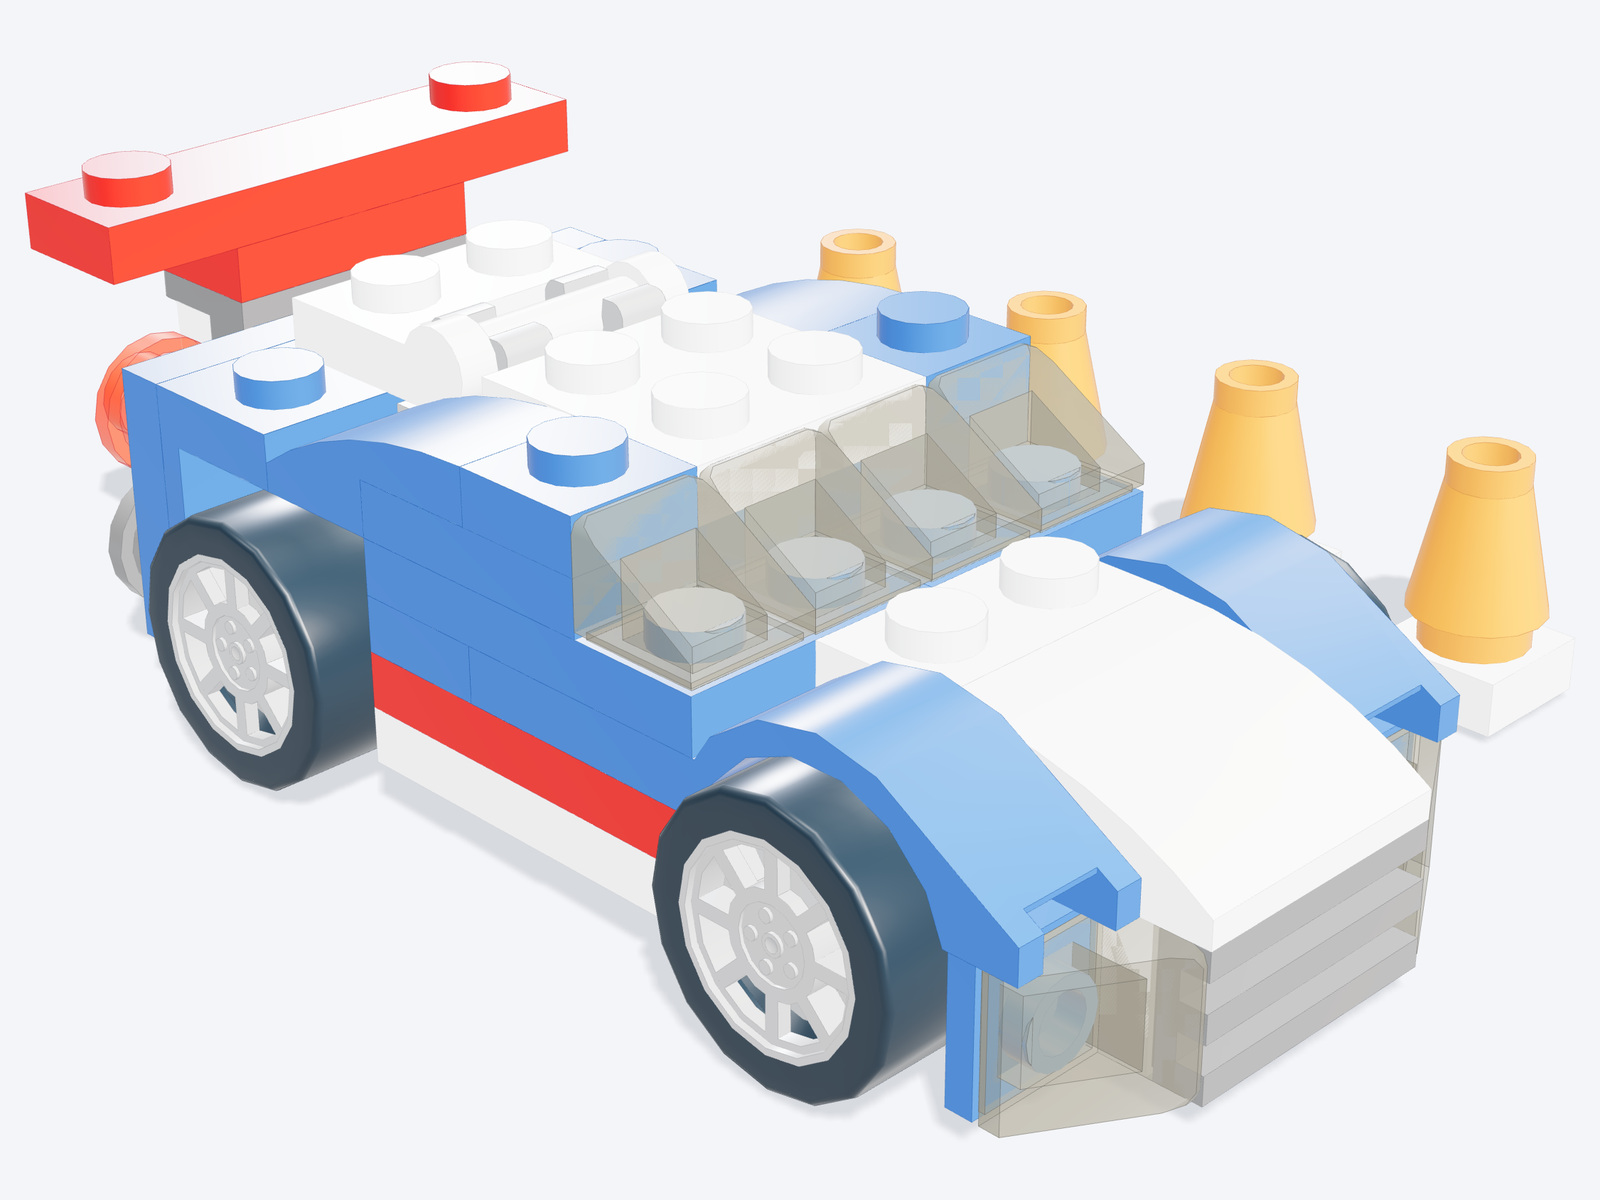
\includegraphics[width=.48\linewidth]{figures/ldraw/print/31027-iso.jpg}
\includegraphics[width=.48\linewidth]{figures/ldraw/print/31027-front.jpg}\\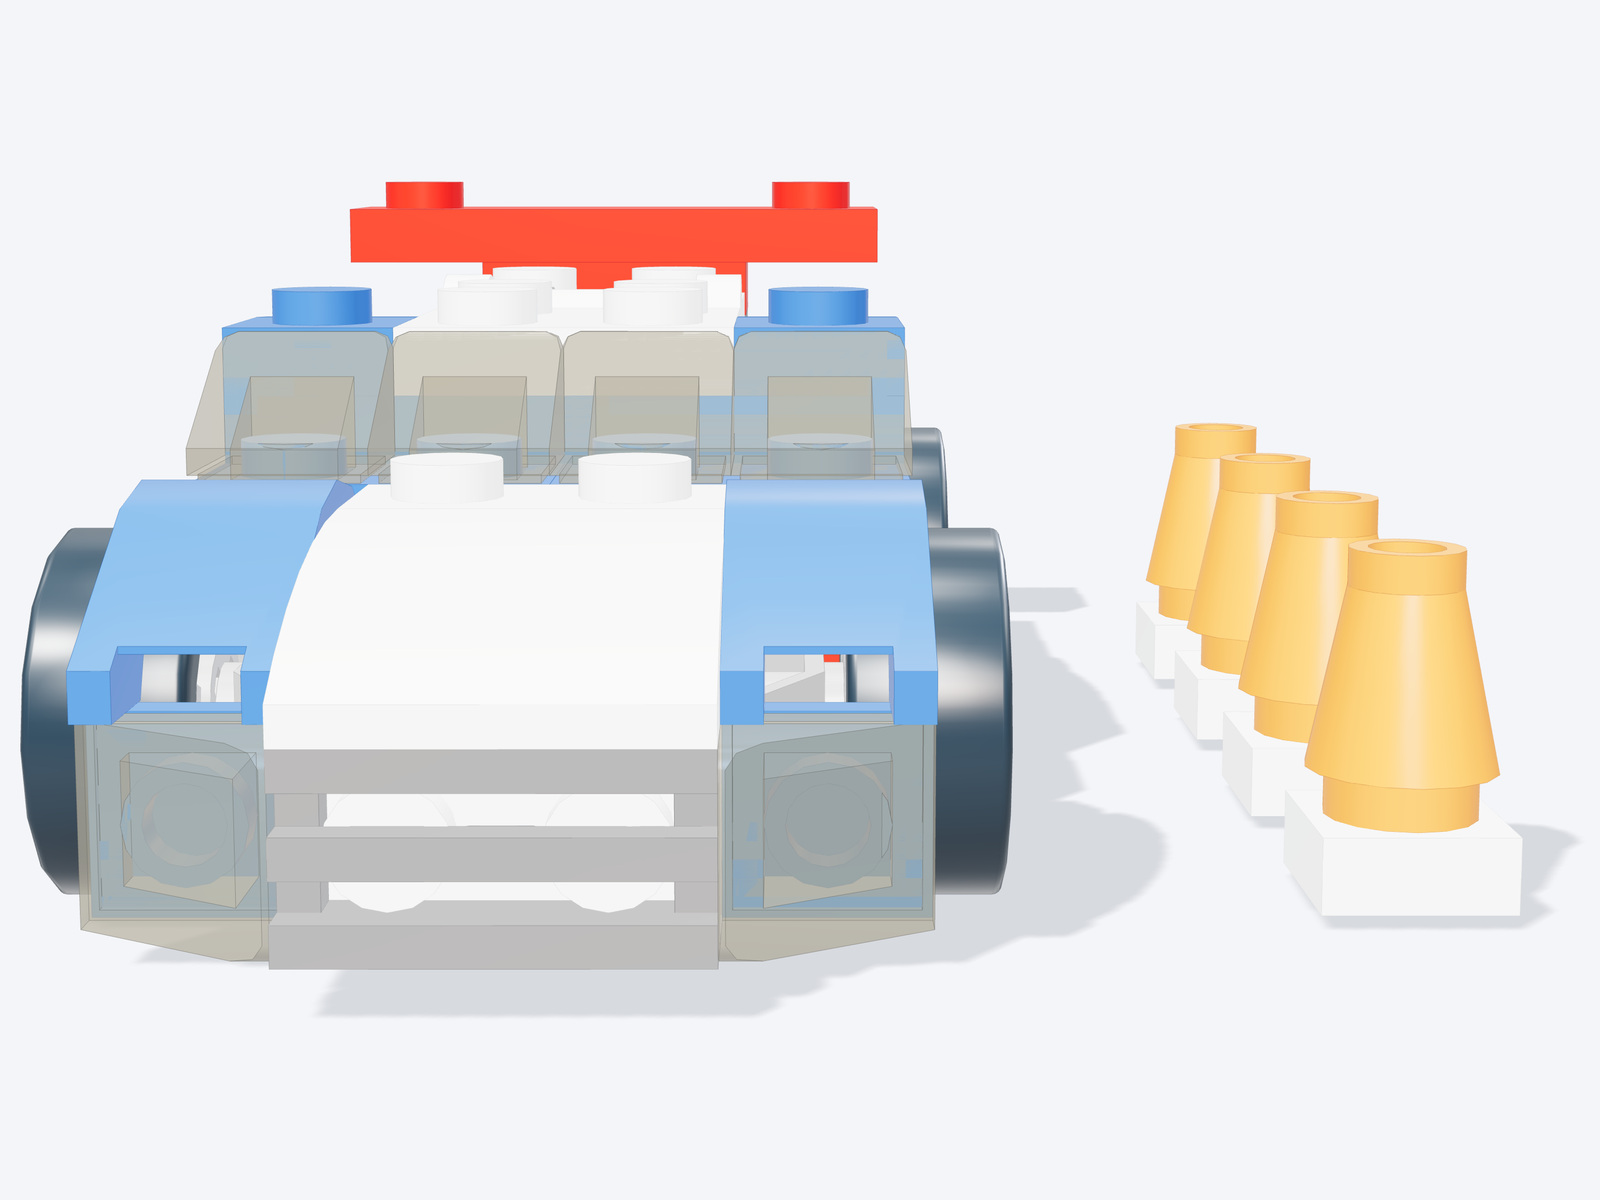
\includegraphics[width=.48\linewidth]{figures/ldraw/print/31027-side.jpg}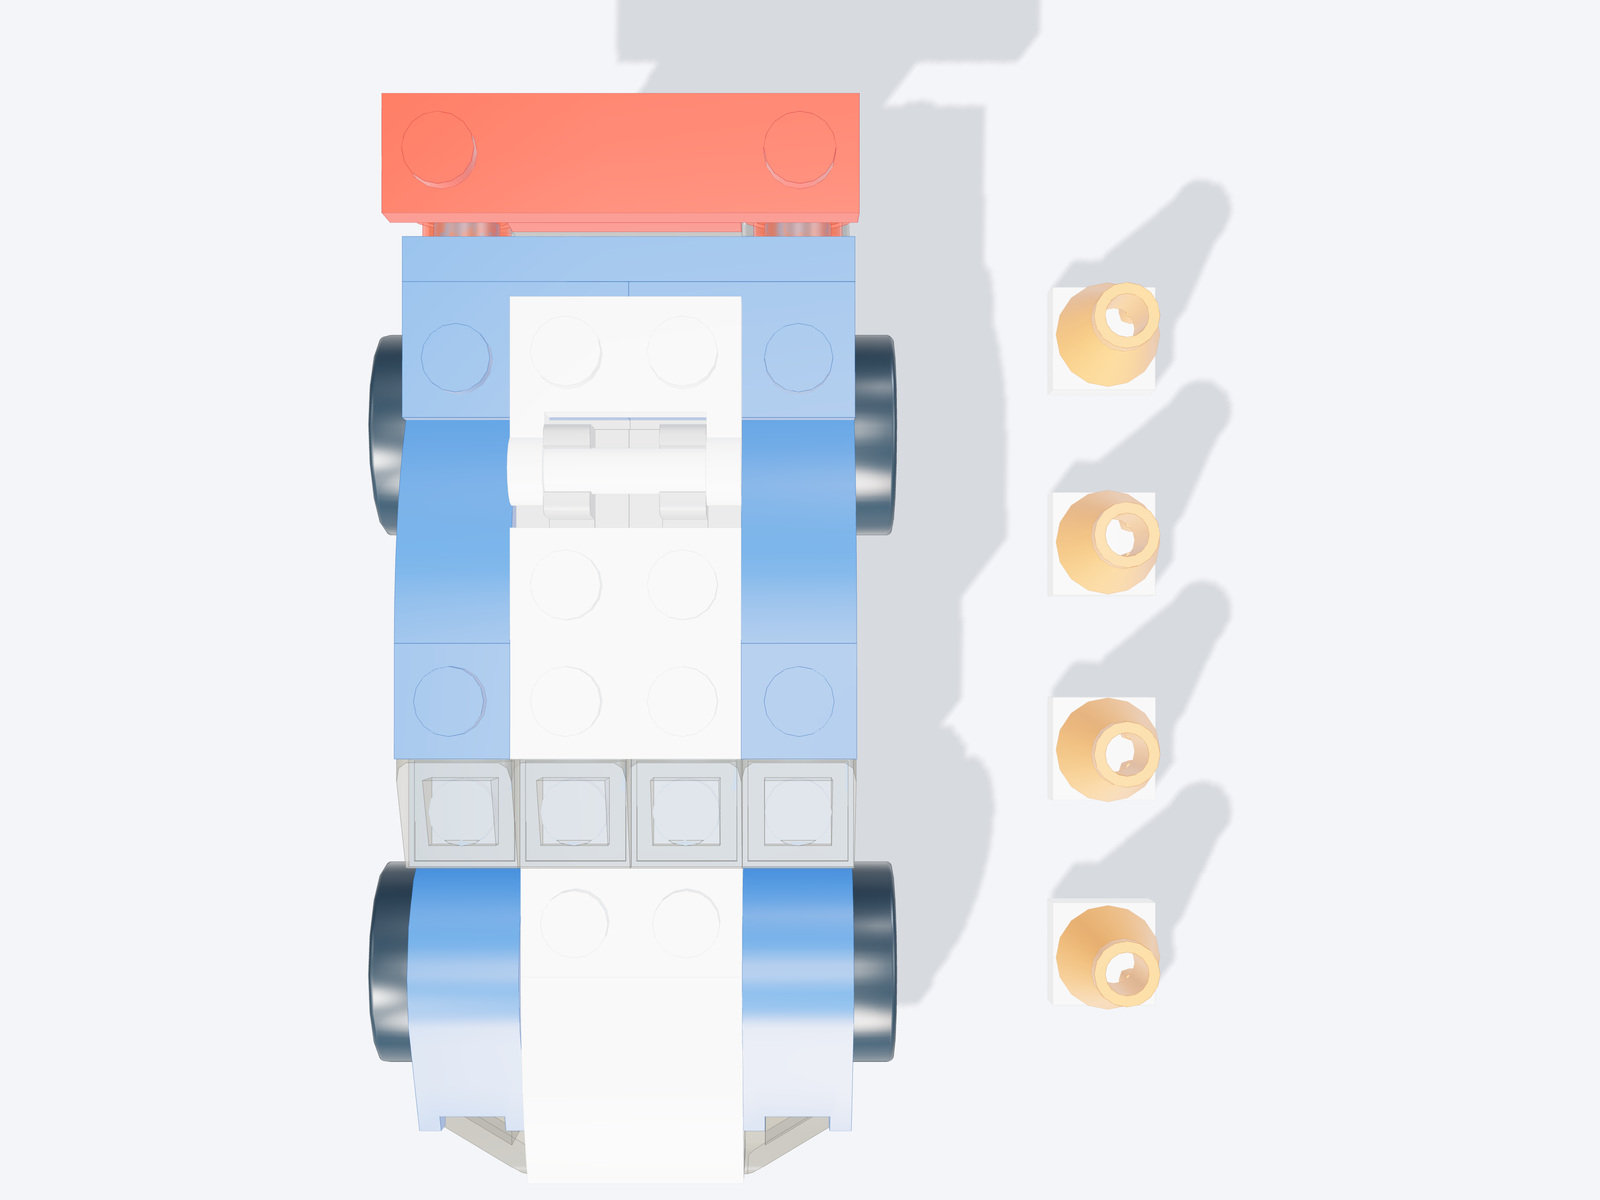
\includegraphics[width=.48\linewidth]{figures/ldraw/print/31027-top.jpg}\end{center}
\paragraph{Attribution.}Merlijn Wissink [legolijntje]. CC BY 2.0.\par\noindent\url{https://library.ldraw.org/omr/sets/223}
\paragraph{Source lock.}\small\texttt{1f1975602ce9a63f2954c8da97f4fc13}\\\texttt{a473f709afa4a25b1022add33b55cfd1}\normalsize
\paragraph{Evidence coverage.}Connector definitions cover 100.00\% of instances. The audit reports 5 recognized-graph components and 0 intersection candidates without a recognized mating pair. 0 instances have no connector definition. These counts do not certify physical defects or gravitational stability.
\paragraph{Instructions.}No author STEP replay or source-order question is provided.
\clearpage\subsection{Numbered visual input and complete question index}
Only relevant numbers are shown. The website can isolate any instance; public visual tasks provide their own numbered images. The following entries give every English prompt, all choice options, compact public evidence and the reference output. Raw repeated connector records and full action fact sets remain in the versioned JSON.
\begin{center}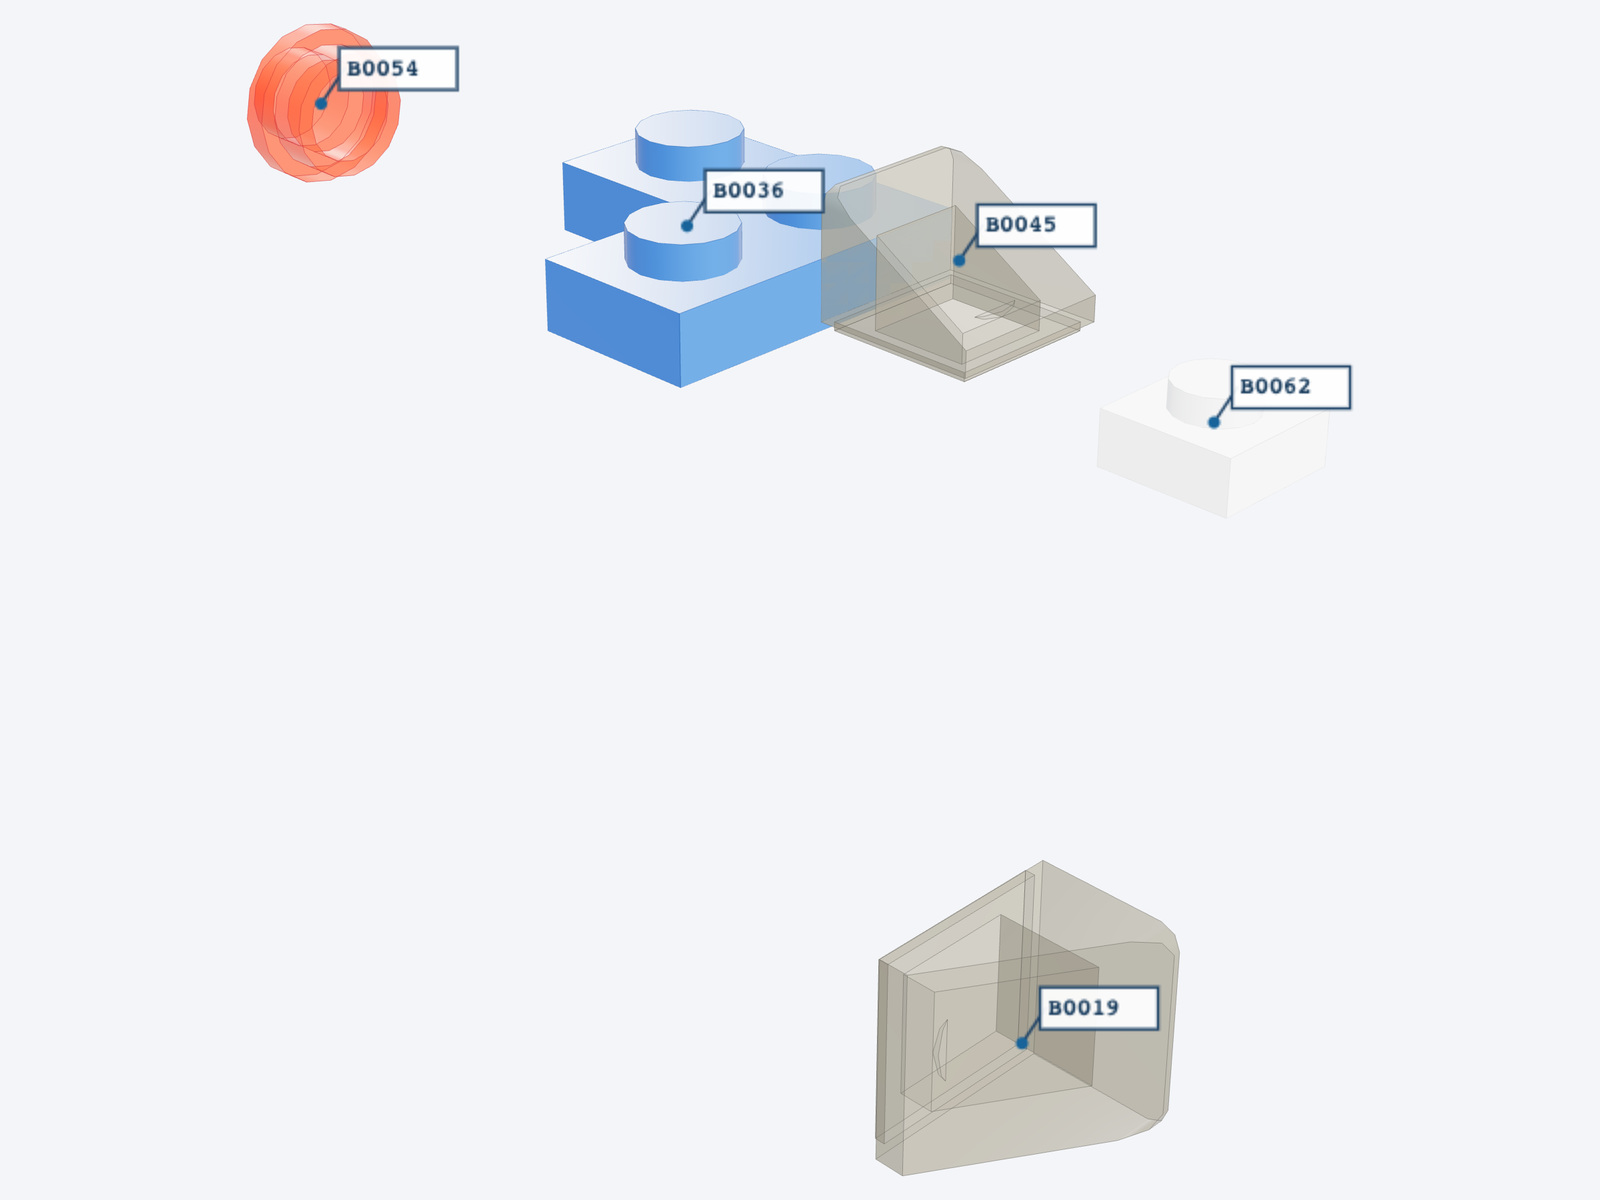
\includegraphics[width=.55\linewidth]{figures/ldraw/print/31027-numbered.jpg}\end{center}
\begin{enumerate}
\item \textbf{color-1}. Identify the original color of B0045; numbered isolation is allowed.\par {\small \textit{Input:} Numbered visual input; source attributes are withheld from the model. \par\textit{Options:} A: Trans Red; B: Light Bluish Grey; C: Trans Brown; D: Orange. \par\textit{Reference output:} C.}
\item \textbf{shape-match-1}. Ignoring color and pose, which numbered instance has the same LDraw part type as B0045?\par {\small \textit{Input:} Numbered visual input; source attributes are withheld from the model. \par\textit{Options:} A: B0019; B: B0062; C: B0054; D: B0036. \par\textit{Reference output:} A.}
\item \textbf{distance-1}. Using the supplied geometry bounding-box centers, which candidate is nearest to B0045?\par {\small \textit{Input:} Centers (mm): B0045 = (12, 9.52, 12); B0040 = (12, 9.600012, -8); B0051 = (12, -2.4, -31.2); B0036 = (8, 8.8, 0). \par\textit{Options:} A: B0040; B: B0036; C: B0051. \par\textit{Reference output:} B.}
\item \textbf{color-2}. Identify the original color of B0050; numbered isolation is allowed.\par {\small \textit{Input:} Numbered visual input; source attributes are withheld from the model. \par\textit{Options:} A: Black; B: White; C: Red; D: Light Bluish Grey. \par\textit{Reference output:} B.}
\item \textbf{shape-match-2}. Ignoring color and pose, which numbered instance has the same LDraw part type as B0050?\par {\small \textit{Input:} Numbered visual input; source attributes are withheld from the model. \par\textit{Options:} A: B0034; B: B0002; C: B0014; D: B0043. \par\textit{Reference output:} A.}
\item \textbf{distance-2}. Using the supplied geometry bounding-box centers, which candidate is nearest to B0050?\par {\small \textit{Input:} Centers (mm): B0050 = (0, 1.6, -32.000012); B0019 = (-12, -4, 36.72); B0046 = (-12, 12, 4); B0058 = (-8, 2.4, -21.6). \par\textit{Options:} A: B0019; B: B0058; C: B0046. \par\textit{Reference output:} B.}
\item \textbf{interface-1}. Classify the supplied connector record for B0037 and B0059. This does not certify load capacity.\par {\small \textit{Input:} Record: family = axle; connector indices = 1, 0. \par\textit{Options:} A: hinge; B: ball; C: axle; D: fixed. \par\textit{Reference output:} C.}
\item \textbf{interface-2}. Classify the supplied connector record for B0026 and B0027. This does not certify load capacity.\par {\small \textit{Input:} Record: family = fixed; connector indices = 1, 1. \par\textit{Options:} A: ball; B: hinge; C: axle; D: fixed. \par\textit{Reference output:} D.}
\item \textbf{interface-3}. Classify the supplied connector record for B0002 and B0024. This does not certify load capacity.\par {\small \textit{Input:} Record: family = hinge; connector indices = 2, 3. \par\textit{Options:} A: ball; B: hinge; C: axle; D: fixed. \par\textit{Reference output:} B.}
\item \textbf{interface-4}. Classify the supplied connector record for B0060 and B0061. This does not certify load capacity.\par {\small \textit{Input:} Record: family = stud; connector indices = 1, 3. \par\textit{Options:} A: stud; B: hinge; C: fixed; D: axle; E: ball. \par\textit{Reference output:} A.}
\item \textbf{neighbors-1}. Select every candidate directly adjacent to B0012 in the supplied connector graph.\par {\small \textit{Input:} Unique undirected pairs: B0001 / B0012; B0012 / B0031. \par\textit{Options:} A: B0001; B: B0031; C: B0059; D: B0055. \par\textit{Reference output:} A, B.}
\item \textbf{graph-removal-1}. Delete B0012 and its incident edges from this local graph. How many connected components remain? Do not infer physical extractability.\par {\small \textit{Input:} Nodes: B0012, B0001, B0031, B0055, B0059. Unique undirected pairs: B0001 / B0012; B0012 / B0031. \par\textit{Options:} A: 6; B: 4; C: 3; D: 5. \par\textit{Reference output:} B.}
\item \textbf{neighbors-2}. Select every candidate directly adjacent to B0024 in the supplied connector graph.\par {\small \textit{Input:} Unique undirected pairs: B0002 / B0024; B0024 / B0025. \par\textit{Options:} A: B0058; B: B0002; C: B0053; D: B0025. \par\textit{Reference output:} B, D.}
\item \textbf{graph-removal-2}. Delete B0024 and its incident edges from this local graph. How many connected components remain? Do not infer physical extractability.\par {\small \textit{Input:} Nodes: B0024, B0002, B0025, B0053, B0058. Unique undirected pairs: B0002 / B0024; B0024 / B0025. \par\textit{Options:} A: 4; B: 6; C: 5; D: 3. \par\textit{Reference output:} A.}
\item \textbf{evidence-limit-1}. Only source geometry, connector matching and mesh intersection audits are available. Without mass, friction, material or dynamic tests, is gravitational stability established?\par {\small \textit{Input:} Available evidence: Original CAD; Connector inference; Inset-mesh intersection candidates. \par\textit{Options:} A: Not established by this evidence; B: Established. \par\textit{Reference output:} A.}
\item \textbf{restore-instance-1}. The display copy hides B0045. Restore only that numbered instance, preserving all other instances and source poses.\par {\small \textit{Input:} Target: B0045. Action budget: 1. All other instances initially remain visible. \par\textit{Reference output:} restore-B0045.}
\item \textbf{restore-instance-2}. The display copy hides B0050. Restore only that numbered instance, preserving all other instances and source poses.\par {\small \textit{Input:} Target: B0050. Action budget: 1. All other instances initially remain visible. \par\textit{Reference output:} restore-B0050.}
\end{enumerate}
\clearpage
\section{10156: LEGO Truck}
111 source instances; 20 tasks; D1 scale band.

\par\noindent Perspective, front, side and top views follow in reading order. Original source transforms are preserved.
\begin{center}
\includegraphics[width=.48\linewidth]{figures/ldraw/print/10156-iso.jpg}
\includegraphics[width=.48\linewidth]{figures/ldraw/print/10156-front.jpg}\\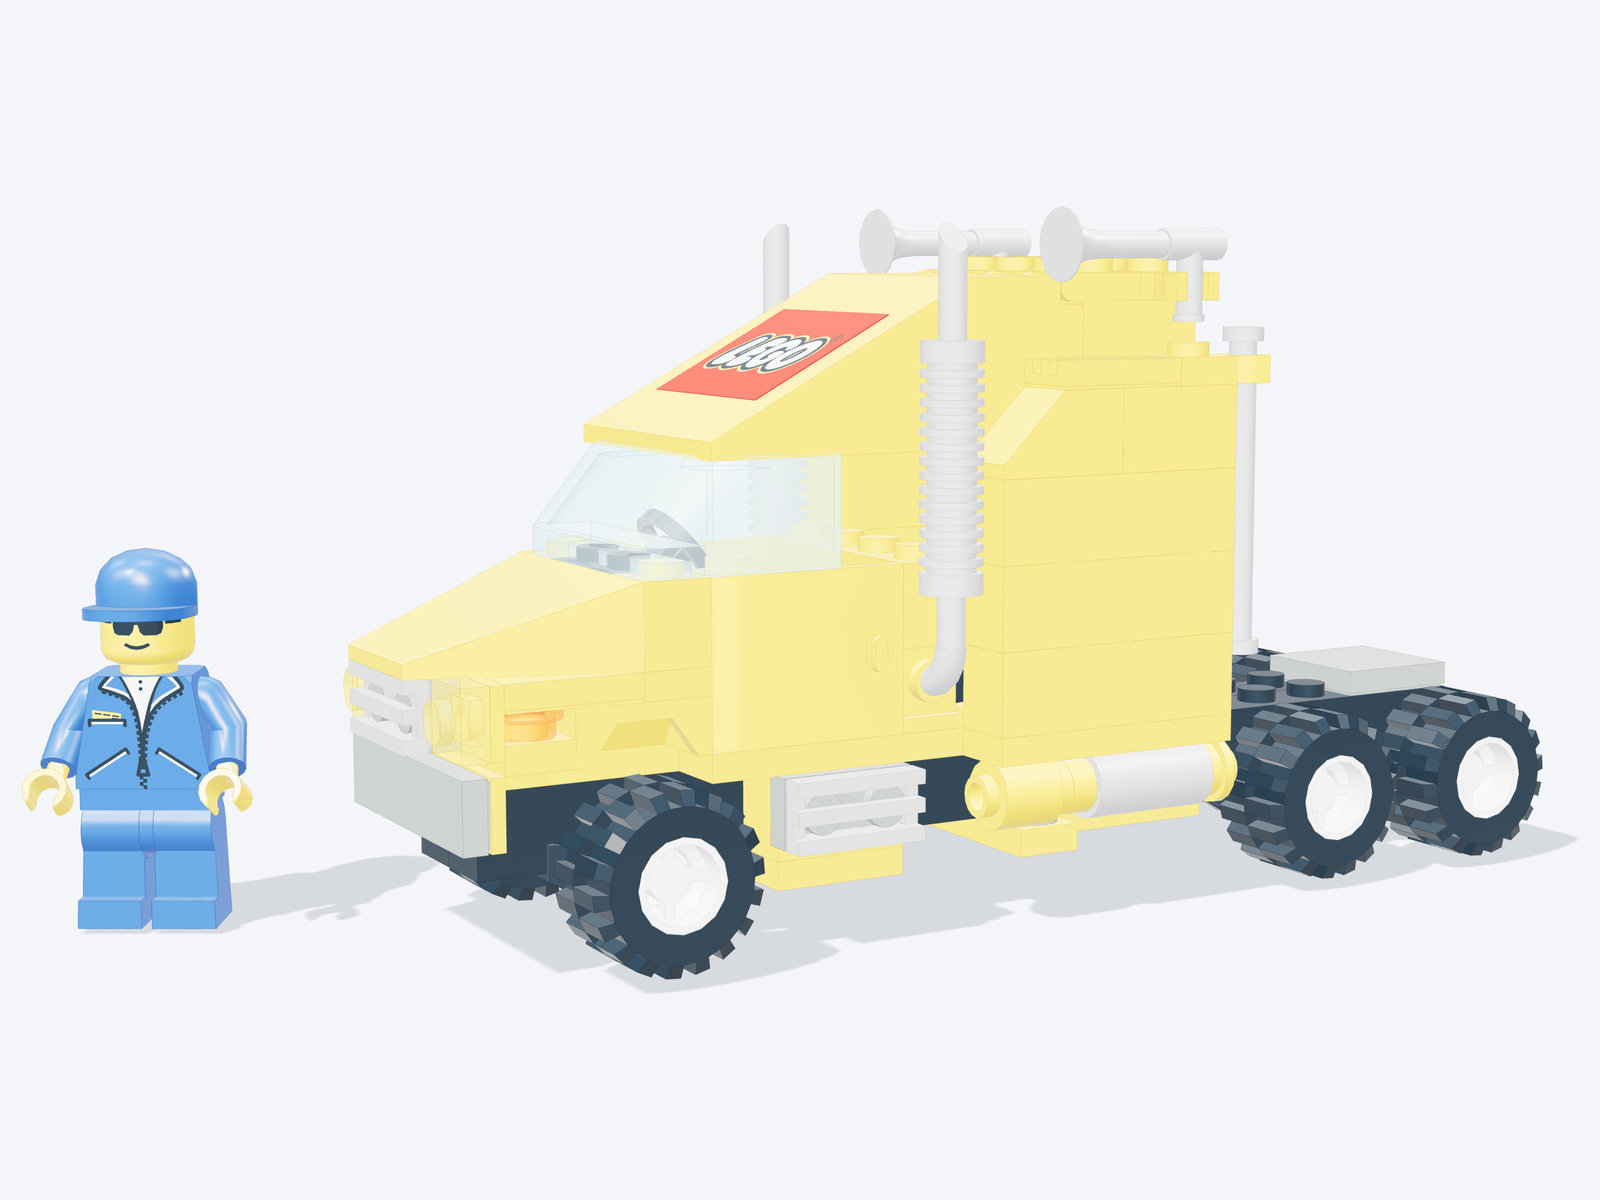
\includegraphics[width=.48\linewidth]{figures/ldraw/print/10156-side.jpg}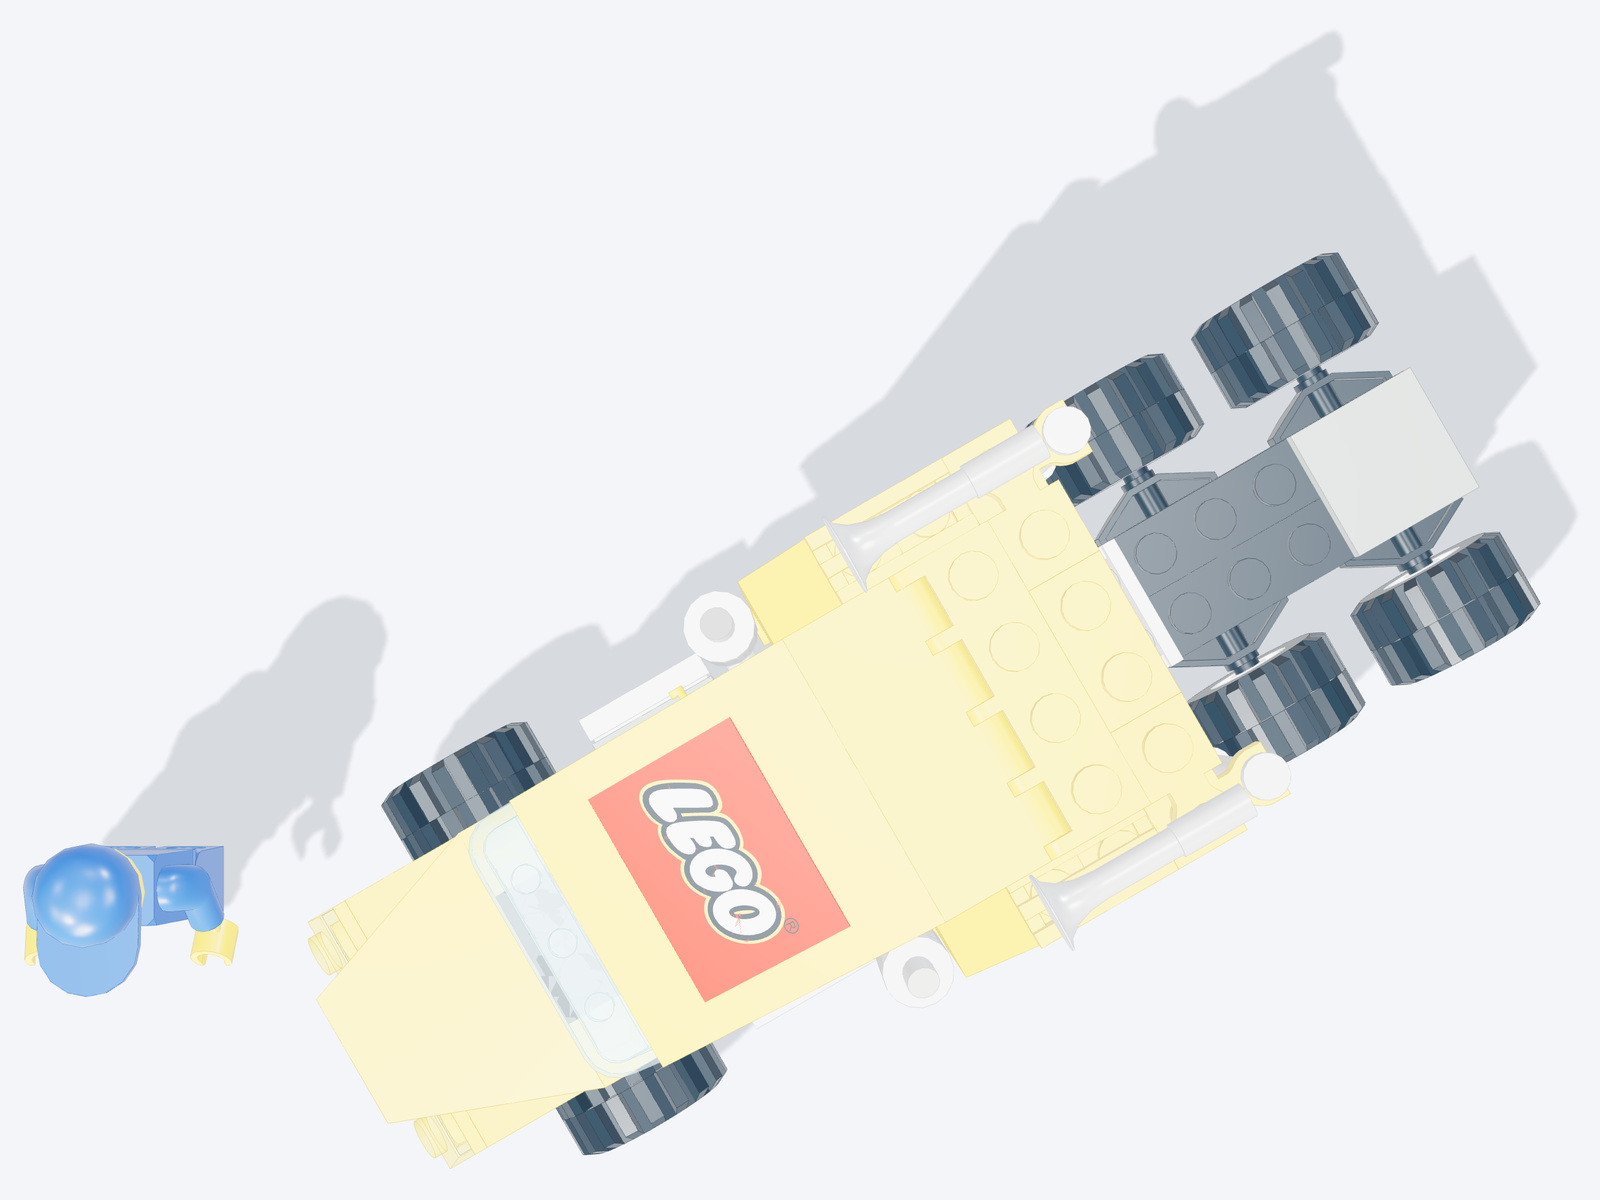
\includegraphics[width=.48\linewidth]{figures/ldraw/print/10156-top.jpg}\end{center}
\paragraph{Attribution.}Robert Paciorek [bercik]. CC BY 2.0.\par\noindent\url{https://library.ldraw.org/omr/sets/659}
\paragraph{Source lock.}\small\texttt{a58a784e6f6ce9d39999db1a4505941b}\\\texttt{5db5ebd1798af979bae891bc520a1a45}\normalsize
\paragraph{Evidence coverage.}Connector definitions cover 99.10\% of instances. The audit reports 3 recognized-graph components and 2 intersection candidates without a recognized mating pair. 1 instances have no connector definition. These counts do not certify physical defects or gravitational stability.
\paragraph{Instructions.}19 expanded author steps.
\clearpage\subsection{Numbered visual input and complete question index}
Only relevant numbers are shown. The website can isolate any instance; public visual tasks provide their own numbered images. The following entries give every English prompt, all choice options, compact public evidence and the reference output. Raw repeated connector records and full action fact sets remain in the versioned JSON.
\begin{center}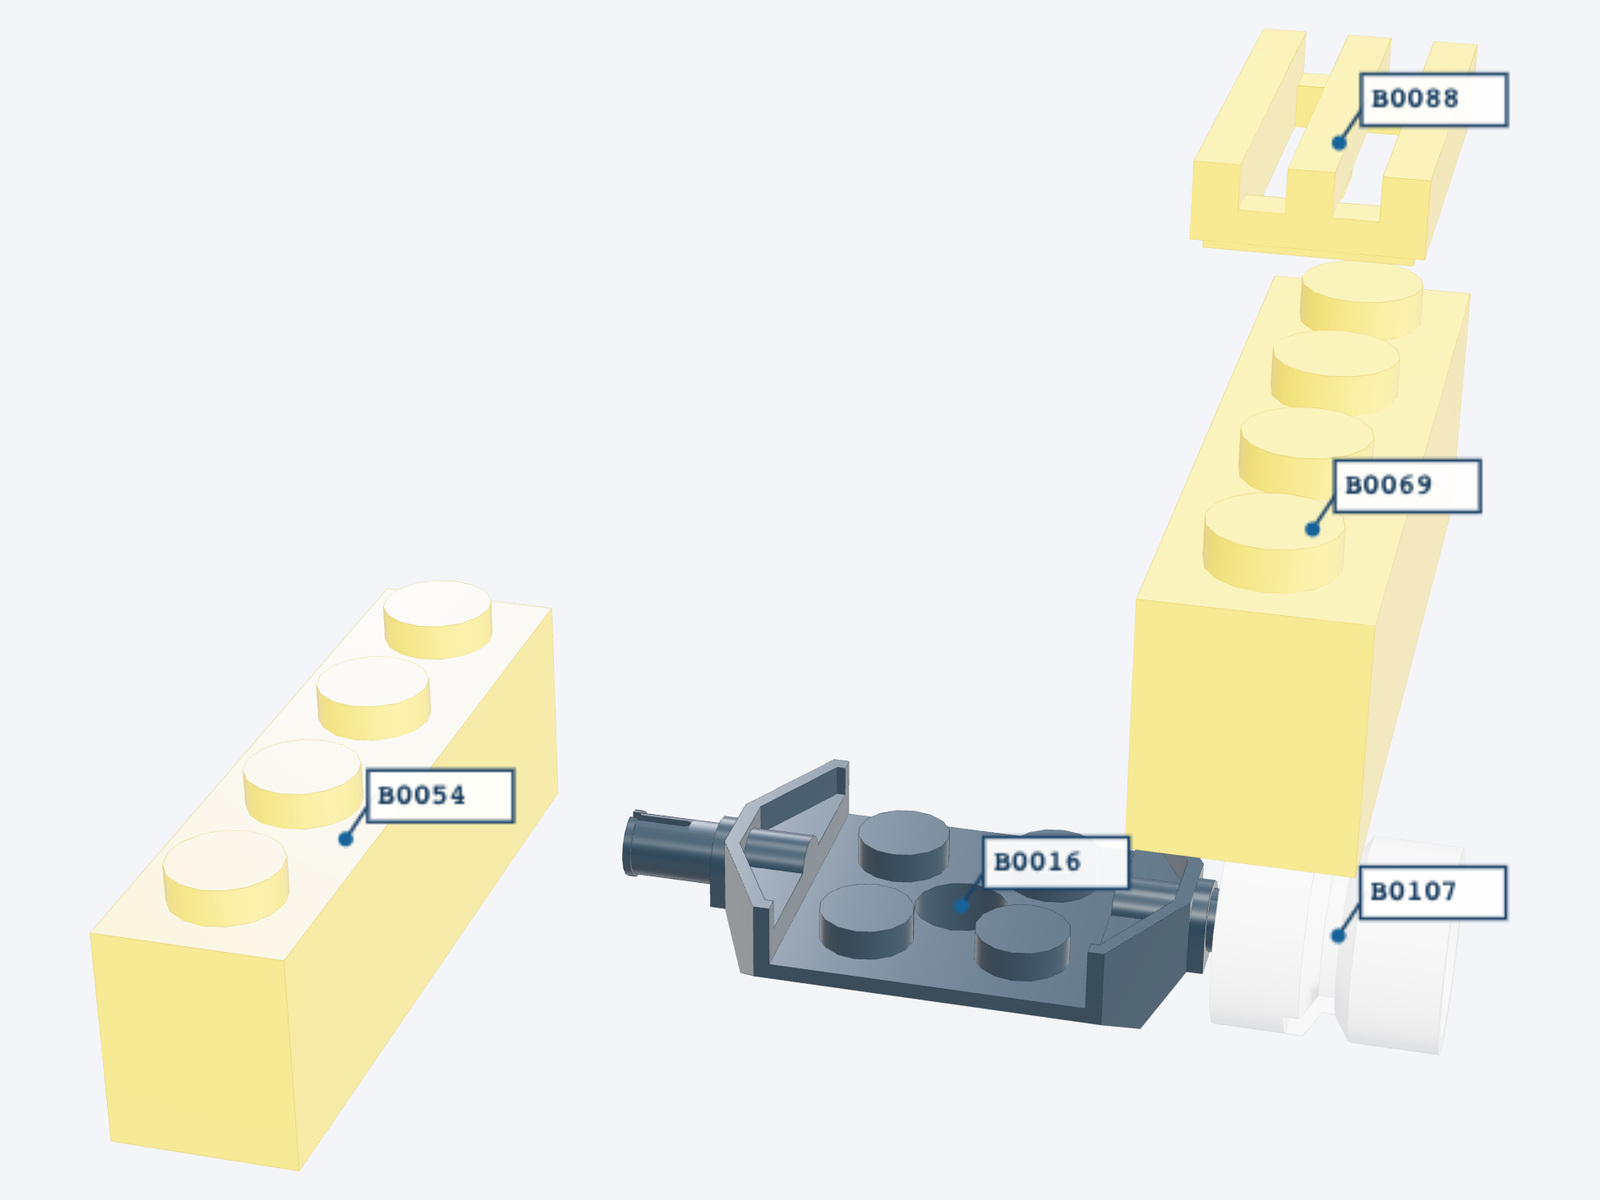
\includegraphics[width=.55\linewidth]{figures/ldraw/print/10156-numbered.jpg}\end{center}
\begin{enumerate}
\item \textbf{color-1}. Identify the original color of B0069; numbered isolation is allowed.\par {\small \textit{Input:} Numbered visual input; source attributes are withheld from the model. \par\textit{Options:} A: Yellow; B: Chrome Silver; C: White; D: Red. \par\textit{Reference output:} A.}
\item \textbf{shape-match-1}. Ignoring color and pose, which numbered instance has the same LDraw part type as B0069?\par {\small \textit{Input:} Numbered visual input; source attributes are withheld from the model. \par\textit{Options:} A: B0107; B: B0016; C: B0054; D: B0088. \par\textit{Reference output:} C.}
\item \textbf{distance-1}. Using the supplied geometry bounding-box centers, which candidate is nearest to B0069?\par {\small \textit{Input:} Centers (mm): B0069 = (68.105528, 47.2, -7.879336); B0045 = (38.606308, 15.2, -36.974207); B0067 = (-3.769975, 28.8, 11.199482); B0093 = (60.18416, 72.8, -26.399917). \par\textit{Options:} A: B0067; B: B0093; C: B0045. \par\textit{Reference output:} B.}
\item \textbf{color-2}. Identify the original color of B0019; numbered isolation is allowed.\par {\small \textit{Input:} Numbered visual input; source attributes are withheld from the model. \par\textit{Options:} A: Light Grey; B: Black; C: Chrome Silver; D: Trans Neon Orange. \par\textit{Reference output:} A.}
\item \textbf{distance-2}. Using the supplied geometry bounding-box centers, which candidate is nearest to B0019?\par {\small \textit{Input:} Centers (mm): B0019 = (-7.119767, 18.4, 12.499461); B0086 = (65.426448, 48, -52.520376); B0101 = (97.003521, 10.8, -69.827264); B0031 = (38.3926, 15.2, 4.949118). \par\textit{Options:} A: B0031; B: B0101; C: B0086. \par\textit{Reference output:} A.}
\item \textbf{interface-1}. Classify the supplied connector record for B0099 and B0018. This does not certify load capacity.\par {\small \textit{Input:} Record: family = axle; connector indices = 0, 1. \par\textit{Options:} A: hinge; B: axle; C: fixed; D: ball. \par\textit{Reference output:} B.}
\item \textbf{interface-2}. Classify the supplied connector record for B0107 and B0108. This does not certify load capacity.\par {\small \textit{Input:} Record: family = fixed; connector indices = 2, 1. \par\textit{Options:} A: fixed; B: ball; C: hinge; D: axle. \par\textit{Reference output:} A.}
\item \textbf{interface-3}. Classify the supplied connector record for B0004 and B0010. This does not certify load capacity.\par {\small \textit{Input:} Record: family = hinge; connector indices = 2, 1. \par\textit{Options:} A: axle; B: hinge; C: fixed; D: ball. \par\textit{Reference output:} B.}
\item \textbf{interface-4}. Classify the supplied connector record for B0080 and B0088. This does not certify load capacity.\par {\small \textit{Input:} Record: family = stud; connector indices = 3, 1. \par\textit{Options:} A: ball; B: stud; C: fixed; D: hinge; E: axle. \par\textit{Reference output:} B.}
\item \textbf{neighbors-1}. Select every candidate directly adjacent to B0105 in the supplied connector graph.\par {\small \textit{Input:} Unique undirected pairs: B0016 / B0105; B0105 / B0106. \par\textit{Options:} A: B0098; B: B0106; C: B0016; D: B0006. \par\textit{Reference output:} B, C.}
\item \textbf{graph-removal-1}. Delete B0105 and its incident edges from this local graph. How many connected components remain? Do not infer physical extractability.\par {\small \textit{Input:} Nodes: B0105, B0016, B0106, B0006, B0098. Unique undirected pairs: B0016 / B0105; B0105 / B0106. \par\textit{Options:} A: 3; B: 6; C: 5; D: 4. \par\textit{Reference output:} D.}
\item \textbf{neighbors-2}. Select every candidate directly adjacent to B0070 in the supplied connector graph.\par {\small \textit{Input:} Unique undirected pairs: B0063 / B0070; B0070 / B0082. \par\textit{Options:} A: B0076; B: B0063; C: B0082; D: B0035. \par\textit{Reference output:} B, C.}
\item \textbf{graph-removal-2}. Delete B0070 and its incident edges from this local graph. How many connected components remain? Do not infer physical extractability.\par {\small \textit{Input:} Nodes: B0070, B0082, B0063, B0076, B0035. Unique undirected pairs: B0063 / B0070; B0070 / B0082. \par\textit{Options:} A: 6; B: 4; C: 5; D: 3. \par\textit{Reference output:} B.}
\item \textbf{coverage-1}. Which numbered instance lacks a connector definition in the coverage record, so this audit cannot establish that it is floating?\par {\small \textit{Input:} Definition coverage: B0111 = unsupported; B0069 = supported; B0019 = supported; B0081 = supported. \par\textit{Options:} A: B0069; B: B0111; C: B0019; D: B0081. \par\textit{Reference output:} B.}
\item \textbf{evidence-limit-1}. Only source geometry, connector matching and mesh intersection audits are available. Without mass, friction, material or dynamic tests, is gravitational stability established?\par {\small \textit{Input:} Available evidence: Original CAD; Connector inference; Inset-mesh intersection candidates. \par\textit{Options:} A: Established; B: Not established by this evidence. \par\textit{Reference output:} B.}
\item \textbf{source-step-1}. At which expanded author step does B0075 first appear in the supplied source-step table? Source order is not a collision-free assembly proof.\par {\small \textit{Input:} Expanded author records: step 1: B0001; step 14: B0075. \par\textit{Options:} A: 16; B: 13; C: 15; D: 14. \par\textit{Reference output:} D.}
\item \textbf{source-step-2}. At which expanded author step does B0050 first appear in the supplied source-step table? Source order is not a collision-free assembly proof.\par {\small \textit{Input:} Expanded author records: step 1: B0001; step 10: B0050. \par\textit{Options:} A: 12; B: 11; C: 9; D: 10. \par\textit{Reference output:} D.}
\item \textbf{source-sequence-1}. Reveal the supplied source-step window in author order. Actions change visibility only, without simulating insertion trajectories.\par {\small \textit{Input:} Source window: step-1: B0001, B0002, B0003, B0004, B0005, B0006, B0007, B0008, B0009, B0010; step-2: B0011, B0012, B0013; step-3: B0014, B0015; step-4: B0016, B0017, B0018, B0019; step-5: B0020, B0021, B0022; step-6: B0023, B0024, B0025, B0026, B0027, B0028, B0029. Action budget: 6. \par\textit{Reference output:} step-1, step-2, step-3, step-4, step-5, step-6.}
\item \textbf{restore-instance-1}. The display copy hides B0069. Restore only that numbered instance, preserving all other instances and source poses.\par {\small \textit{Input:} Target: B0069. Action budget: 1. All other instances initially remain visible. \par\textit{Reference output:} restore-B0069.}
\item \textbf{restore-instance-2}. The display copy hides B0019. Restore only that numbered instance, preserving all other instances and source poses.\par {\small \textit{Input:} Target: B0019. Action budget: 1. All other instances initially remain visible. \par\textit{Reference output:} restore-B0019.}
\end{enumerate}
\clearpage
\section{42102: Mini CLAAS XERION}
129 source instances; 17 tasks; D1 scale band.

\par\noindent Perspective, front, side and top views follow in reading order. Original source transforms are preserved.
\begin{center}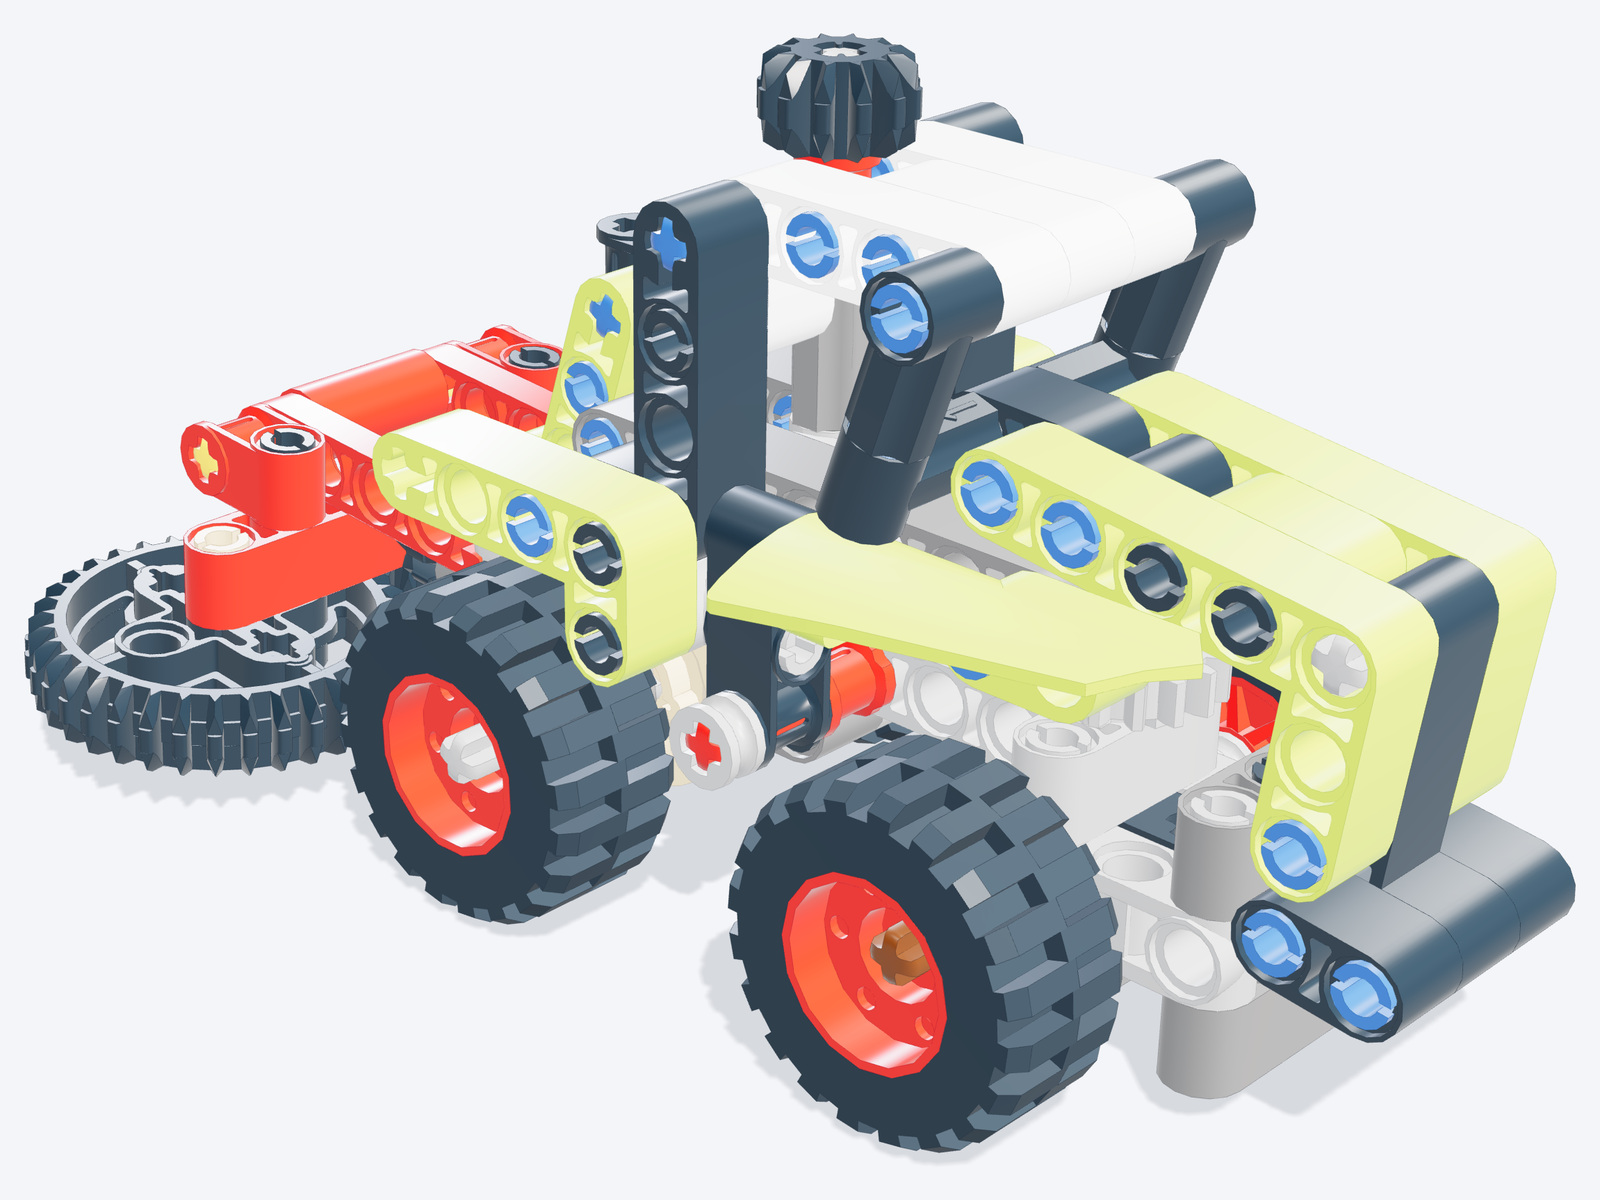
\includegraphics[width=.48\linewidth]{figures/ldraw/print/omr-42102-iso.jpg}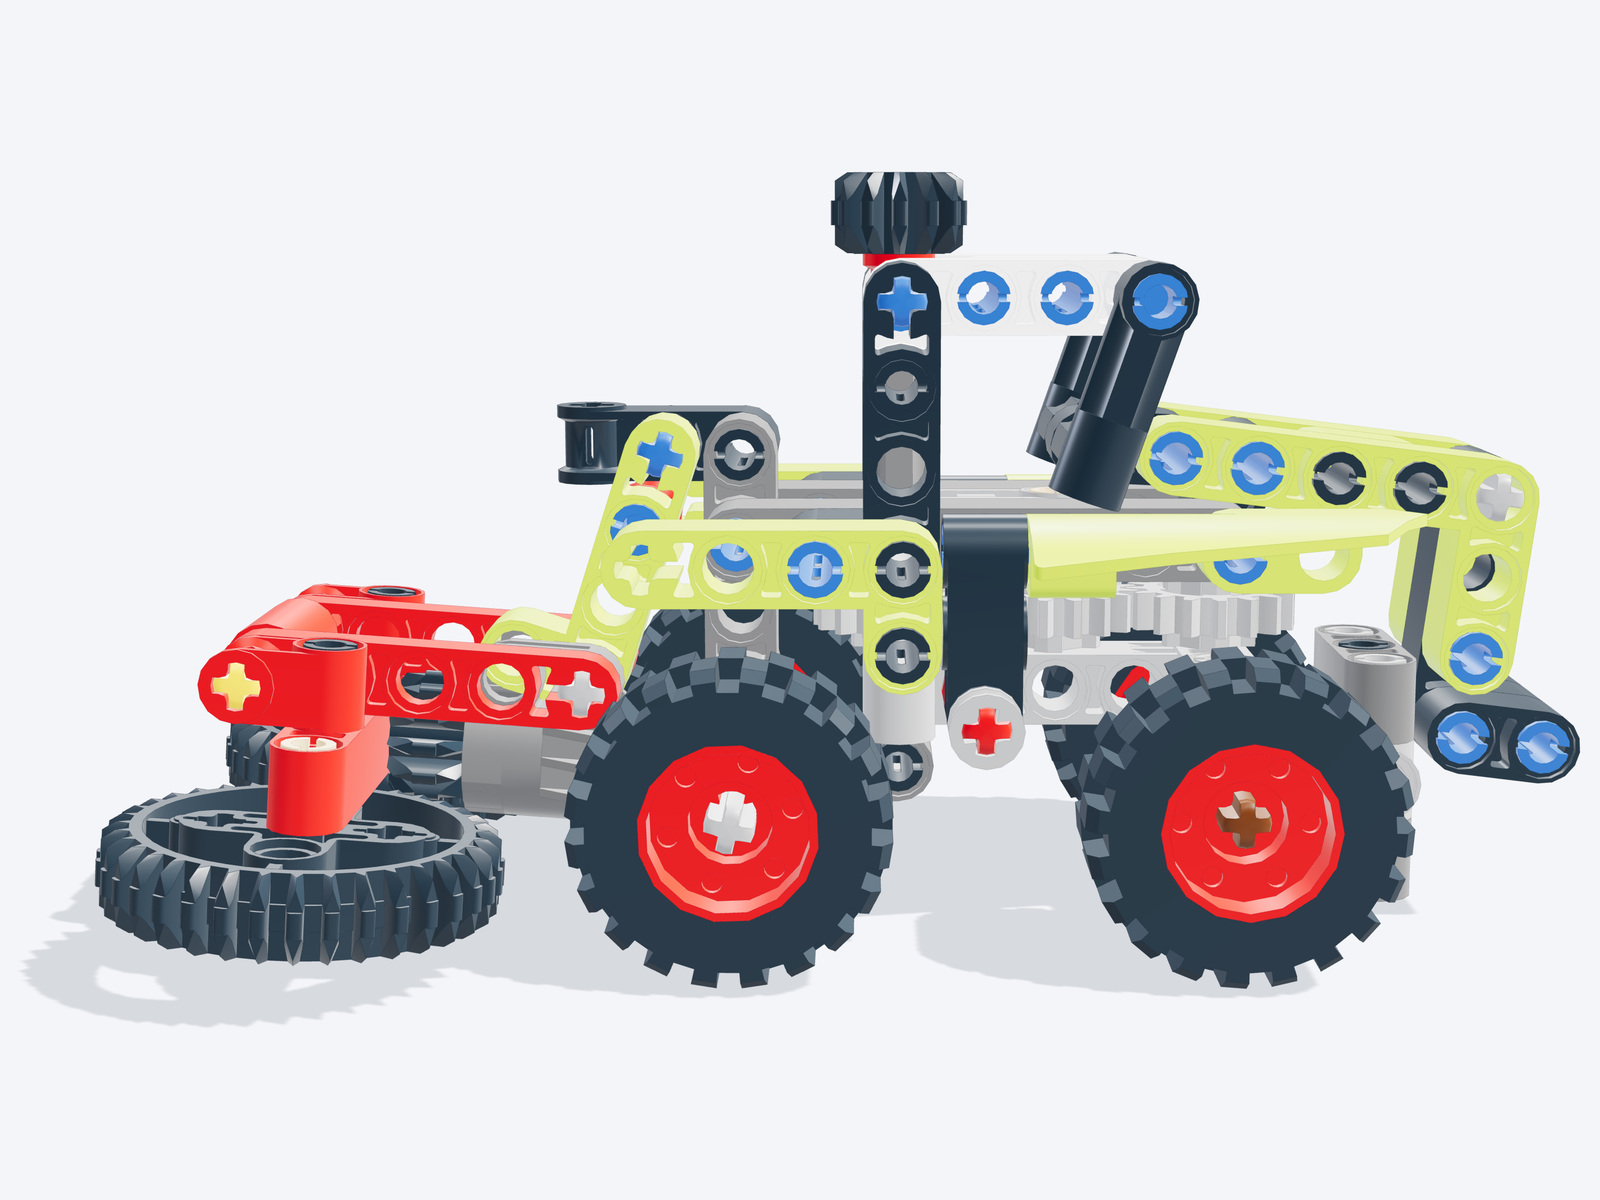
\includegraphics[width=.48\linewidth]{figures/ldraw/print/omr-42102-front.jpg}\\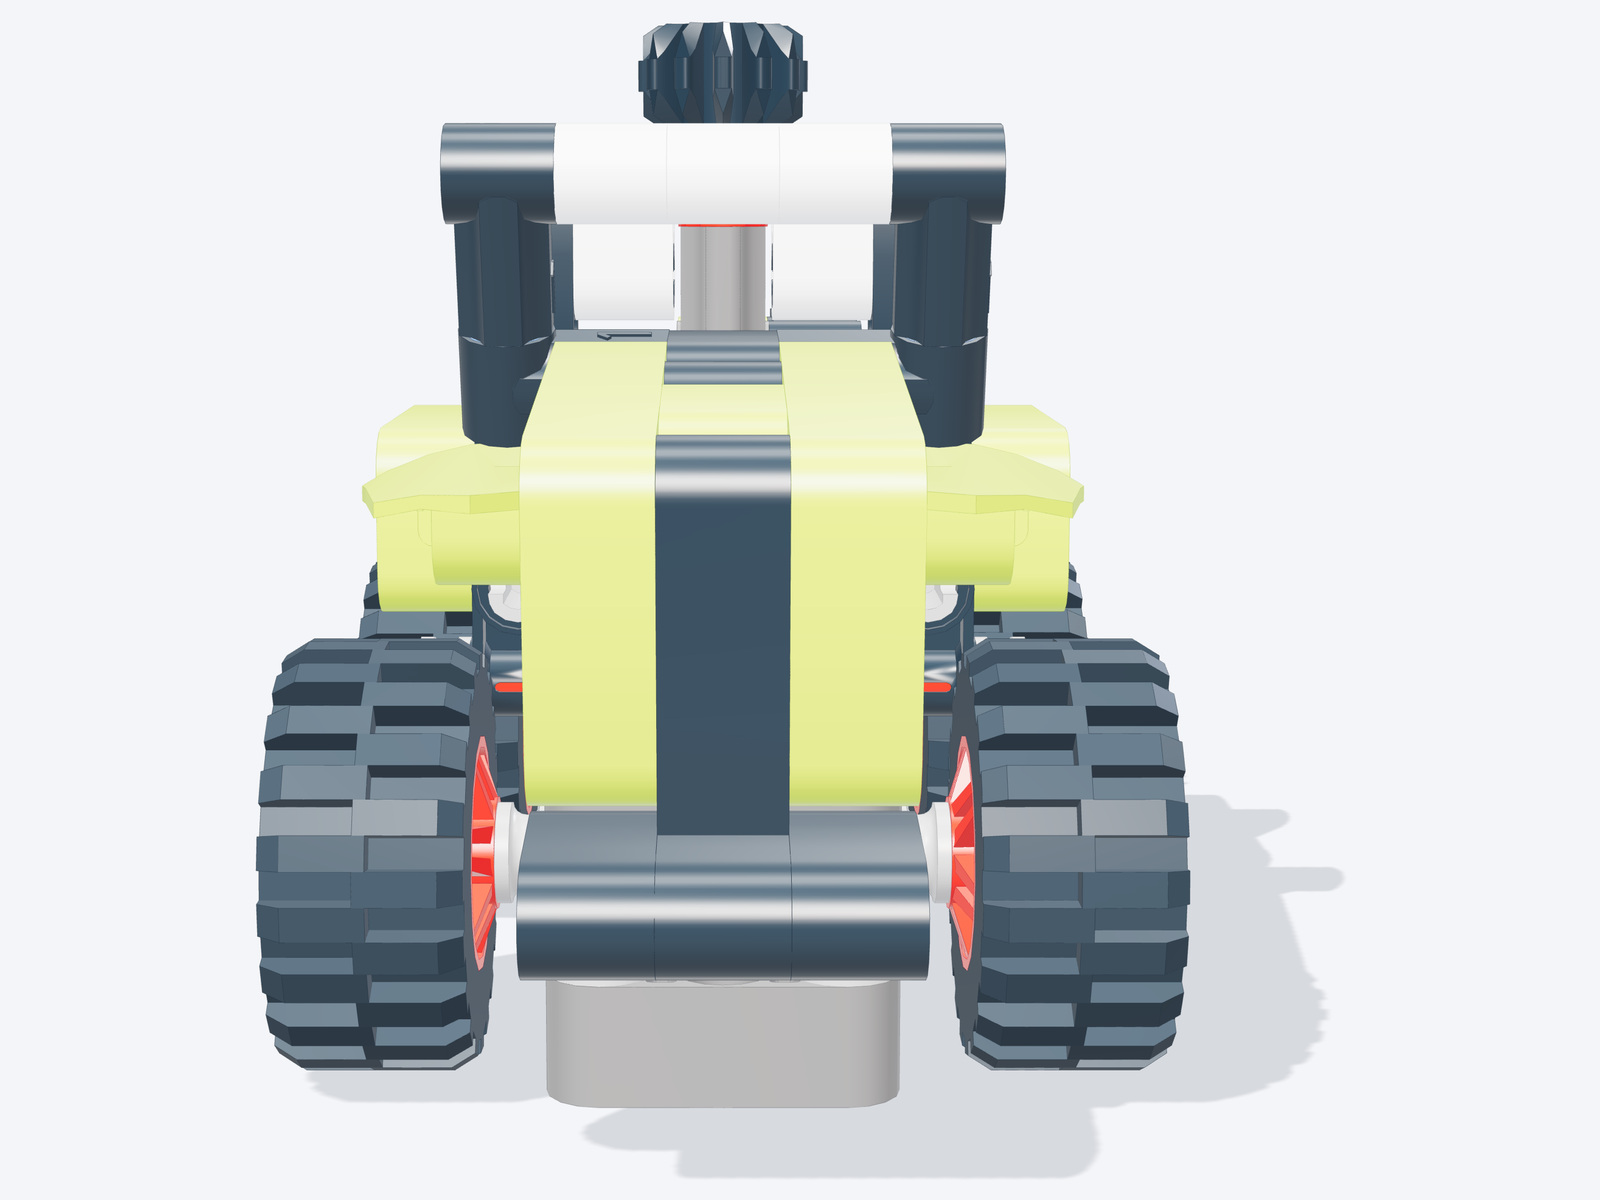
\includegraphics[width=.48\linewidth]{figures/ldraw/print/omr-42102-side.jpg}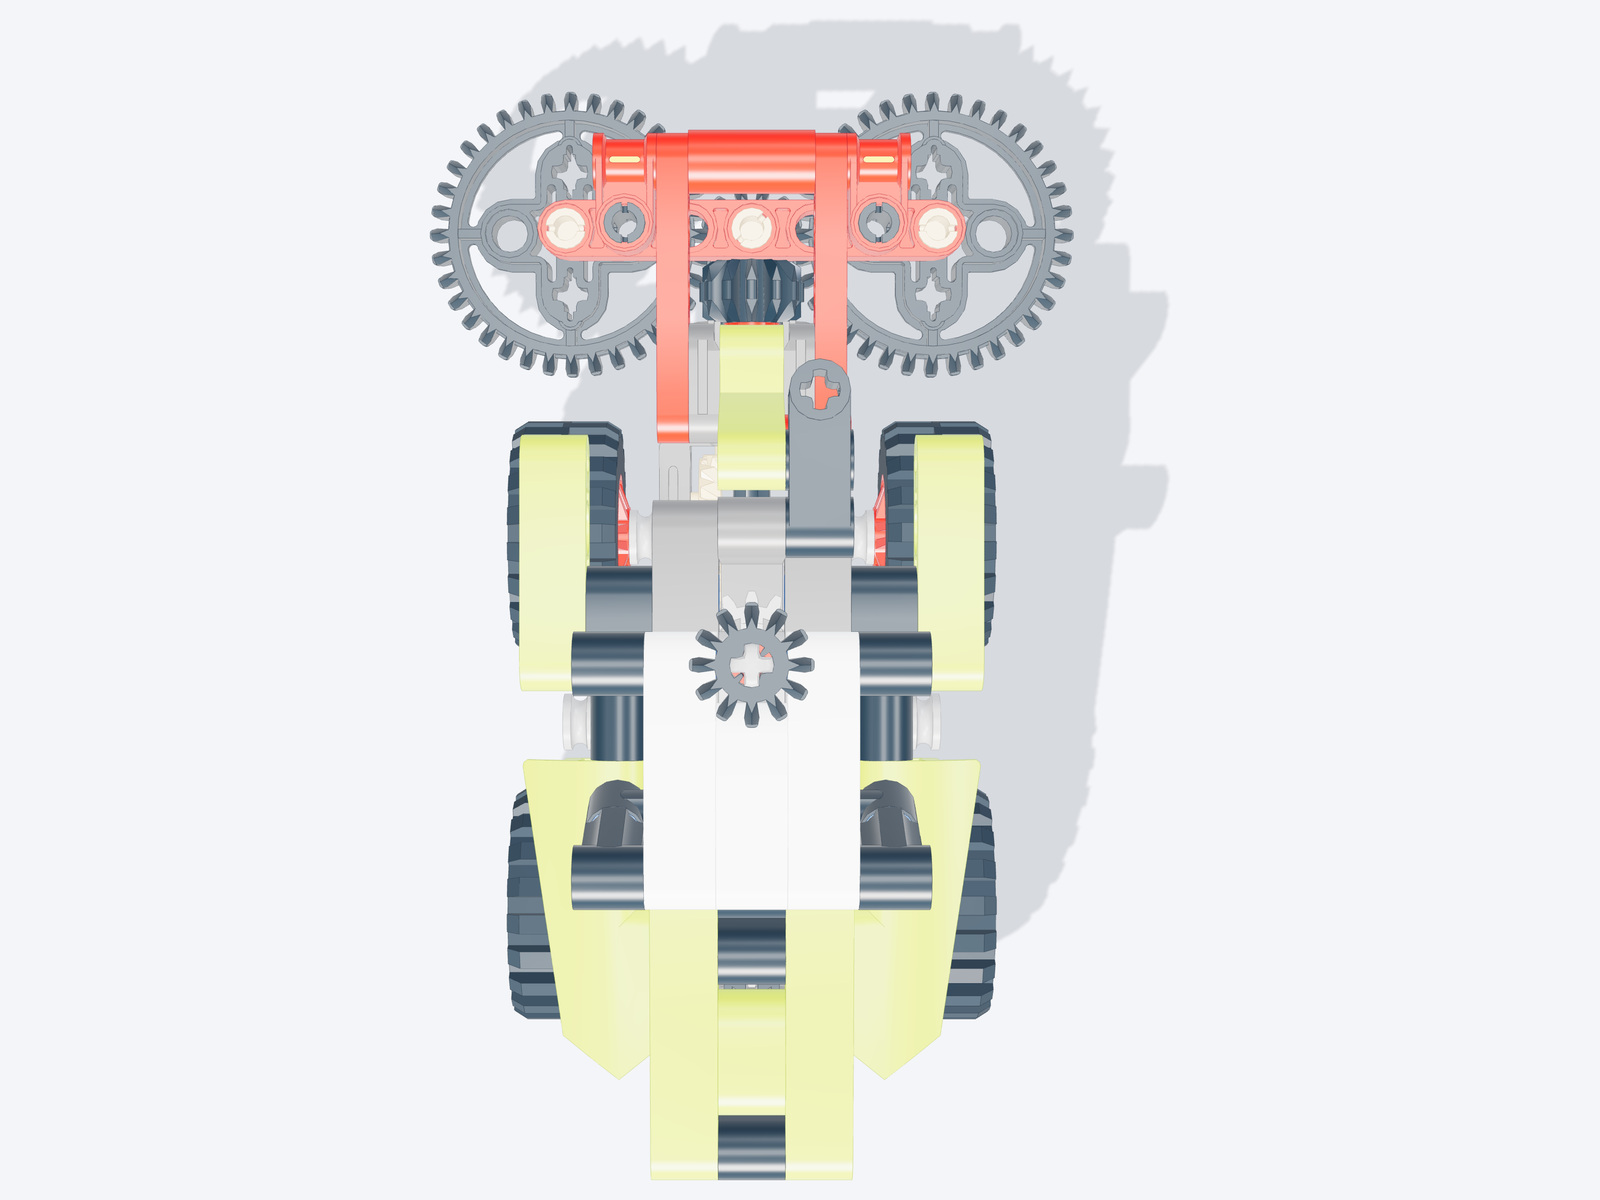
\includegraphics[width=.48\linewidth]{figures/ldraw/print/omr-42102-top.jpg}\end{center}
\paragraph{Attribution.}Max Martin Richter [MMR1988]. CC BY 2.0.\par\noindent\url{https://library.ldraw.org/library/omr/42102-1.mpd}
\paragraph{Source lock.}\small\texttt{096deaf98e20c3e65b547c91e972005d}\\\texttt{853b1b1c3cf7a619910682e6fe2d2deb}\normalsize
\paragraph{Evidence coverage.}Connector definitions cover 95.35\% of instances. The audit reports 8 recognized-graph components and 0 intersection candidates without a recognized mating pair. 6 instances have no connector definition. These counts do not certify physical defects or gravitational stability.
\paragraph{Instructions.}56 expanded author steps.
\clearpage\subsection{Numbered visual input and complete question index}
Only relevant numbers are shown. The website can isolate any instance; public visual tasks provide their own numbered images. The following entries give every English prompt, all choice options, compact public evidence and the reference output. Raw repeated connector records and full action fact sets remain in the versioned JSON.
\begin{center}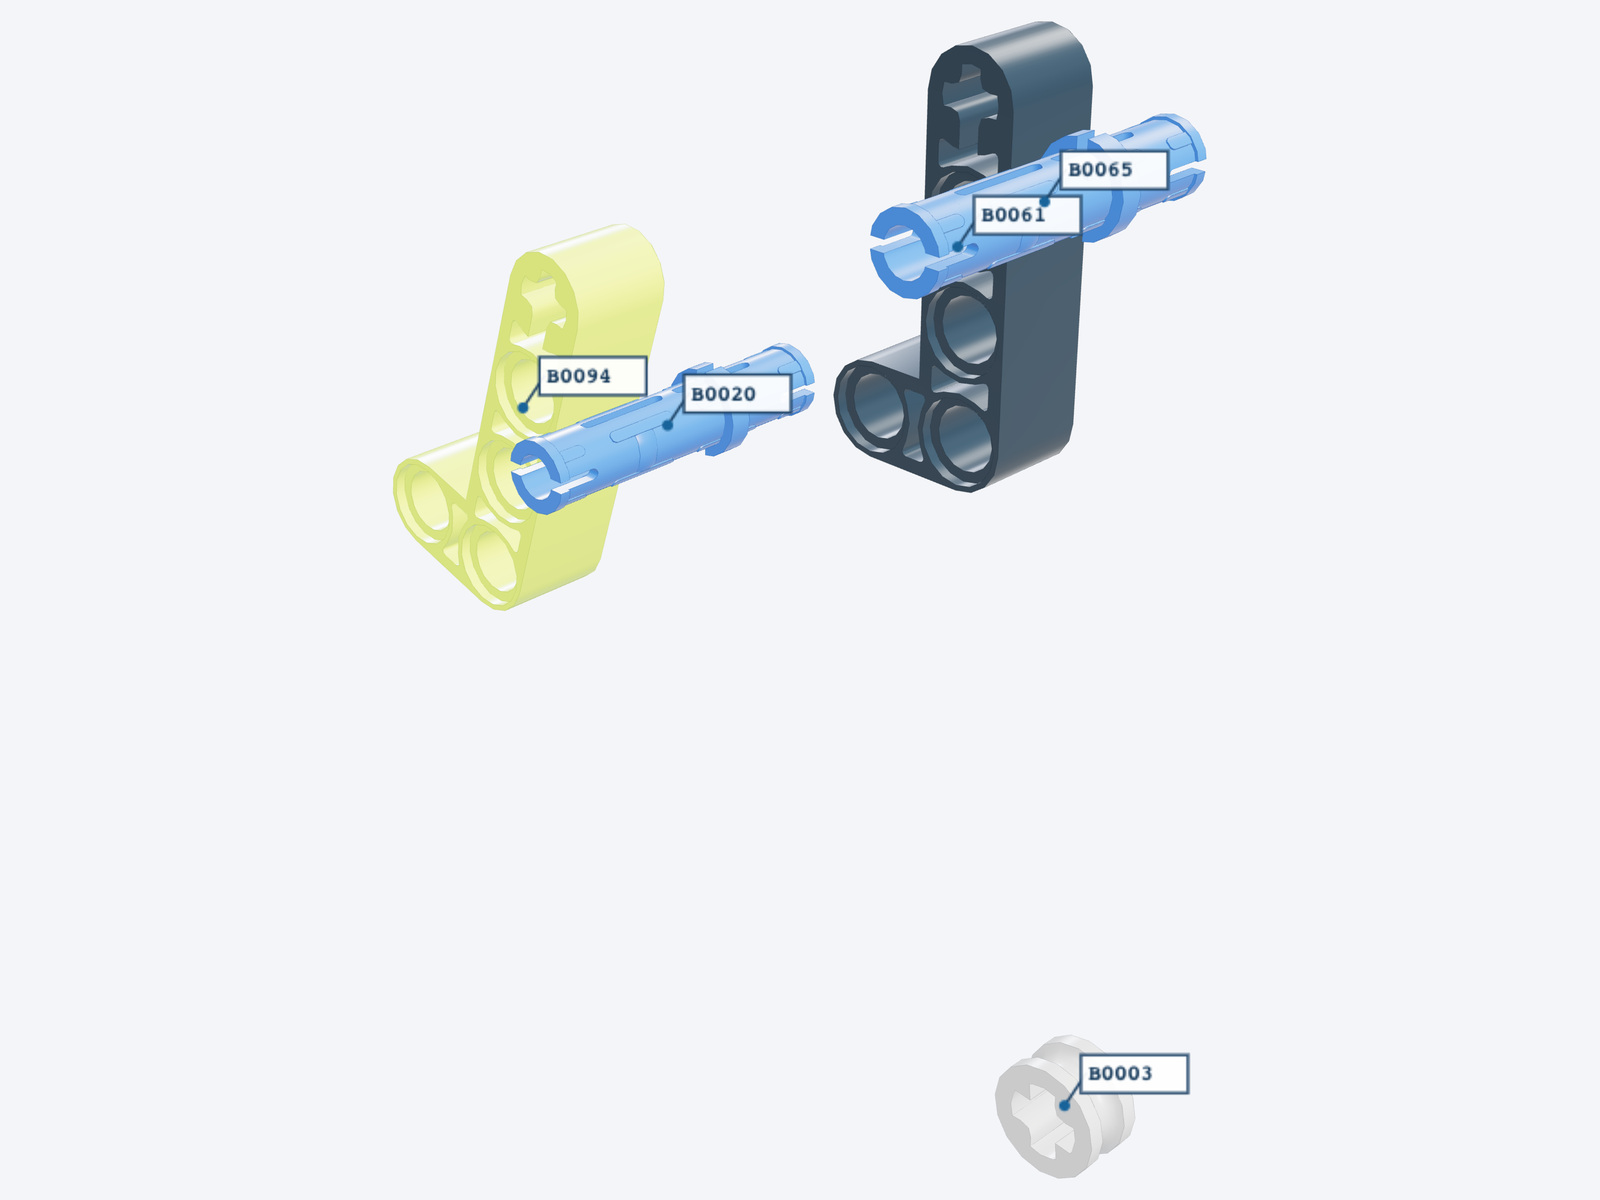
\includegraphics[width=.55\linewidth]{figures/ldraw/print/omr-42102-numbered.jpg}\end{center}
\begin{enumerate}
\item \textbf{color-1}. Identify the original color of B0094; numbered isolation is allowed.\par {\small \textit{Input:} Numbered visual input; source attributes are withheld from the model. \par\textit{Options:} A: Light Bluish Grey; B: Black; C: Red; D: Lime. \par\textit{Reference output:} D.}
\item \textbf{shape-match-1}. Ignoring color and pose, which numbered instance has the same LDraw part type as B0094?\par {\small \textit{Input:} Numbered visual input; source attributes are withheld from the model. \par\textit{Options:} A: B0003; B: B0061; C: B0020; D: B0065. \par\textit{Reference output:} B.}
\item \textbf{distance-1}. Using the supplied geometry bounding-box centers, which candidate is nearest to B0094?\par {\small \textit{Input:} Centers (mm): B0094 = (8, 20.569662, -71.488617); B0045 = (8, 28.592, 18.5592); B0019 = (12, 32, -56); B0053 = (8, 32.496, -13.2168). \par\textit{Options:} A: B0045; B: B0019; C: B0053. \par\textit{Reference output:} B.}
\item \textbf{color-2}. Identify the original color of B0088; numbered isolation is allowed.\par {\small \textit{Input:} Numbered visual input; source attributes are withheld from the model. \par\textit{Options:} A: Lime; B: Black; C: Dark Bluish Grey; D: Tan. \par\textit{Reference output:} B.}
\item \textbf{distance-2}. Using the supplied geometry bounding-box centers, which candidate is nearest to B0088?\par {\small \textit{Input:} Centers (mm): B0088 = (8, 1.4752, -75.9456); B0113 = (6, -0.0048, -56.0056); B0059 = (28, 16, -40); B0124 = (31.4, 0, -8). \par\textit{Options:} A: B0059; B: B0113; C: B0124. \par\textit{Reference output:} B.}
\item \textbf{interface-1}. Classify the supplied connector record for B0037 and B0040. This does not certify load capacity.\par {\small \textit{Input:} Record: family = axle; connector indices = 2, 1. \par\textit{Options:} A: hinge; B: ball; C: fixed; D: axle. \par\textit{Reference output:} D.}
\item \textbf{neighbors-1}. Select every candidate directly adjacent to B0118 in the supplied connector graph.\par {\small \textit{Input:} Unique undirected pairs: B0013 / B0118; B0118 / B0119. \par\textit{Options:} A: B0013; B: B0119; C: B0055; D: B0091. \par\textit{Reference output:} A, B.}
\item \textbf{graph-removal-1}. Delete B0118 and its incident edges from this local graph. How many connected components remain? Do not infer physical extractability.\par {\small \textit{Input:} Nodes: B0118, B0013, B0119, B0055, B0091. Unique undirected pairs: B0013 / B0118; B0118 / B0119. \par\textit{Options:} A: 4; B: 3; C: 5; D: 6. \par\textit{Reference output:} A.}
\item \textbf{neighbors-2}. Select every candidate directly adjacent to B0075 in the supplied connector graph.\par {\small \textit{Input:} Unique undirected pairs: B0071 / B0075; B0074 / B0075. \par\textit{Options:} A: B0074; B: B0129; C: B0120; D: B0071. \par\textit{Reference output:} A, D.}
\item \textbf{graph-removal-2}. Delete B0075 and its incident edges from this local graph. How many connected components remain? Do not infer physical extractability.\par {\small \textit{Input:} Nodes: B0075, B0074, B0071, B0129, B0120. Unique undirected pairs: B0071 / B0075; B0074 / B0075. \par\textit{Options:} A: 6; B: 5; C: 4; D: 3. \par\textit{Reference output:} C.}
\item \textbf{coverage-1}. Which numbered instance lacks a connector definition in the coverage record, so this audit cannot establish that it is floating?\par {\small \textit{Input:} Definition coverage: B0009 = unsupported; B0094 = supported; B0088 = supported; B0114 = supported. \par\textit{Options:} A: B0114; B: B0009; C: B0094; D: B0088. \par\textit{Reference output:} B.}
\item \textbf{evidence-limit-1}. Only source geometry, connector matching and mesh intersection audits are available. Without mass, friction, material or dynamic tests, is gravitational stability established?\par {\small \textit{Input:} Available evidence: Original CAD; Connector inference; Inset-mesh intersection candidates. \par\textit{Options:} A: Established; B: Not established by this evidence. \par\textit{Reference output:} B.}
\item \textbf{source-step-1}. At which expanded author step does B0094 first appear in the supplied source-step table? Source order is not a collision-free assembly proof.\par {\small \textit{Input:} Expanded author records: step 1: B0001; step 43: B0094. \par\textit{Options:} A: 45; B: 43; C: 44; D: 42. \par\textit{Reference output:} B.}
\item \textbf{source-step-2}. At which expanded author step does B0078 first appear in the supplied source-step table? Source order is not a collision-free assembly proof.\par {\small \textit{Input:} Expanded author records: step 1: B0001; step 35: B0078. \par\textit{Options:} A: 36; B: 34; C: 35; D: 37. \par\textit{Reference output:} C.}
\item \textbf{source-sequence-1}. Reveal the supplied source-step window in author order. Actions change visibility only, without simulating insertion trajectories.\par {\small \textit{Input:} Source window: step-1: B0001, B0002, B0003; step-2: B0004, B0005; step-3: B0006, B0007, B0008; step-4: B0009, B0010; step-5: B0011, B0012; step-6: B0013, B0014. Action budget: 6. \par\textit{Reference output:} step-1, step-2, step-3, step-4, step-5, step-6.}
\item \textbf{restore-instance-1}. The display copy hides B0094. Restore only that numbered instance, preserving all other instances and source poses.\par {\small \textit{Input:} Target: B0094. Action budget: 1. All other instances initially remain visible. \par\textit{Reference output:} restore-B0094.}
\item \textbf{restore-instance-2}. The display copy hides B0088. Restore only that numbered instance, preserving all other instances and source poses.\par {\small \textit{Input:} Target: B0088. Action budget: 1. All other instances initially remain visible. \par\textit{Reference output:} restore-B0088.}
\end{enumerate}
\clearpage
\section{42020: Twin-Rotor Helicopter}
141 source instances; 14 tasks; D1 scale band.

\par\noindent Perspective, front, side and top views follow in reading order. Original source transforms are preserved.
\begin{center}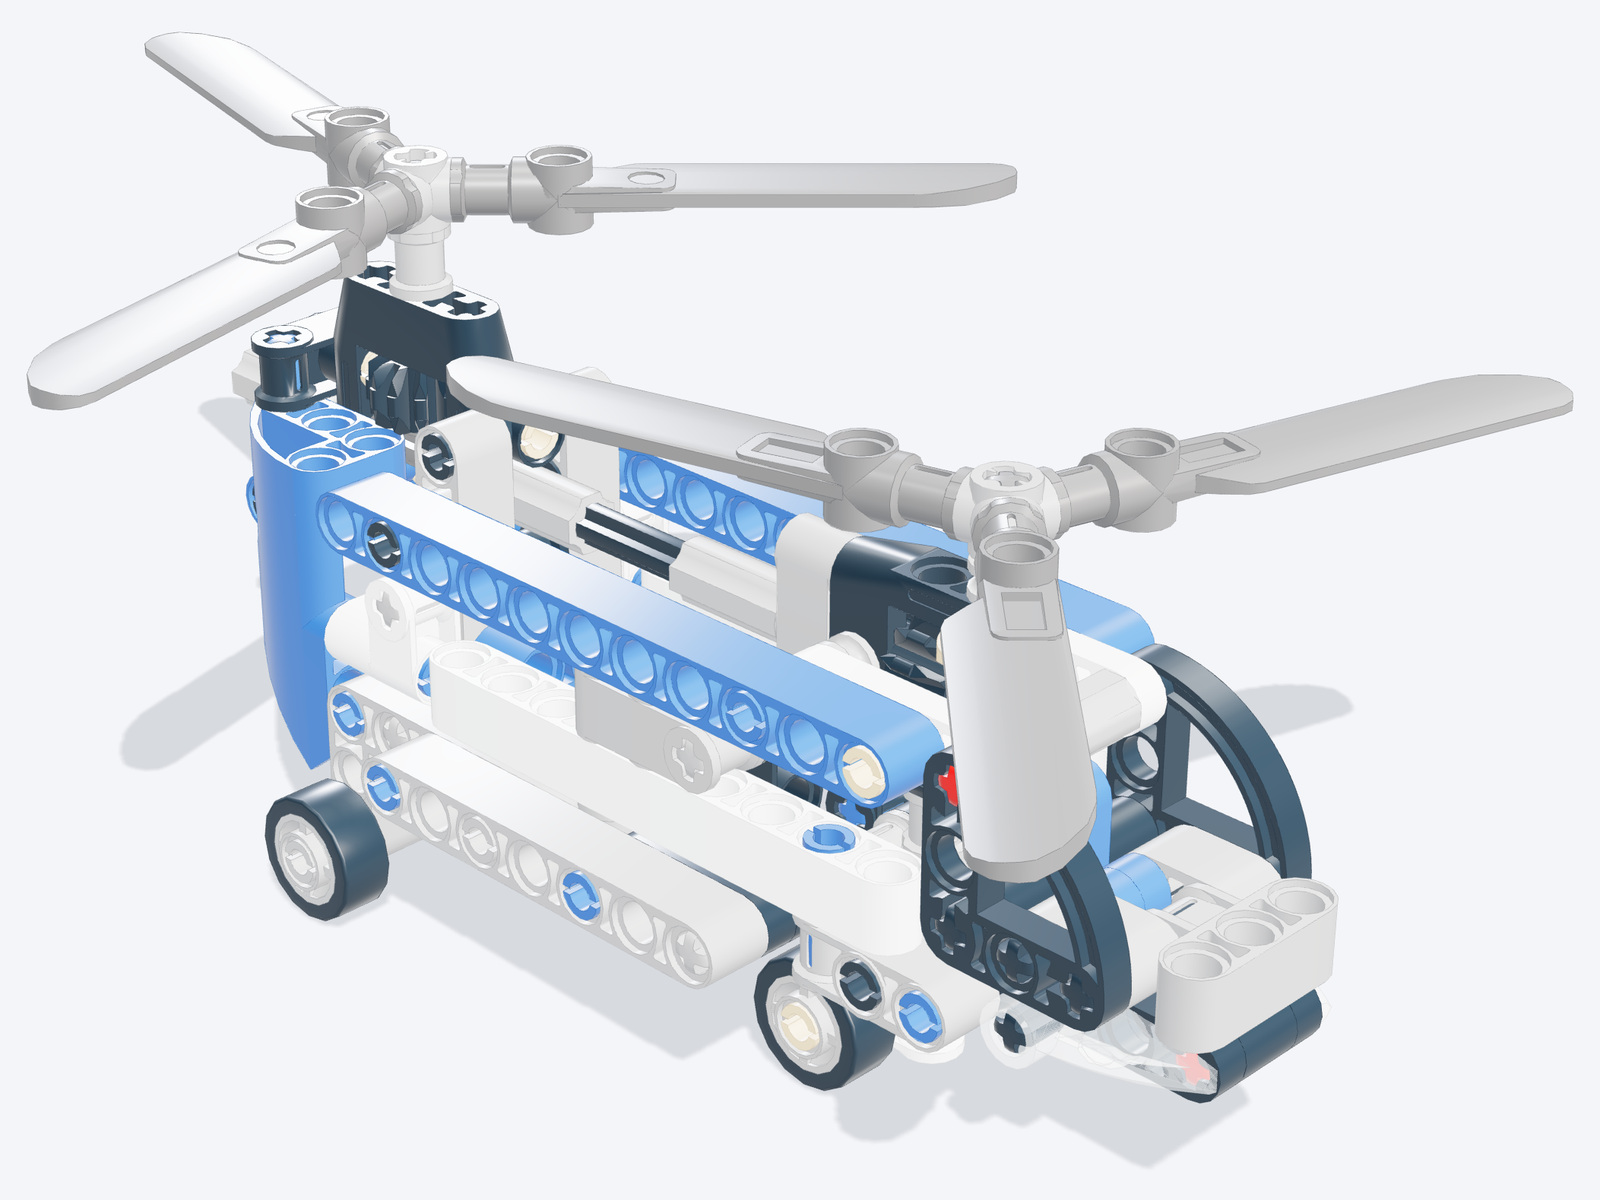
\includegraphics[width=.48\linewidth]{figures/ldraw/print/omr-42020-iso.jpg}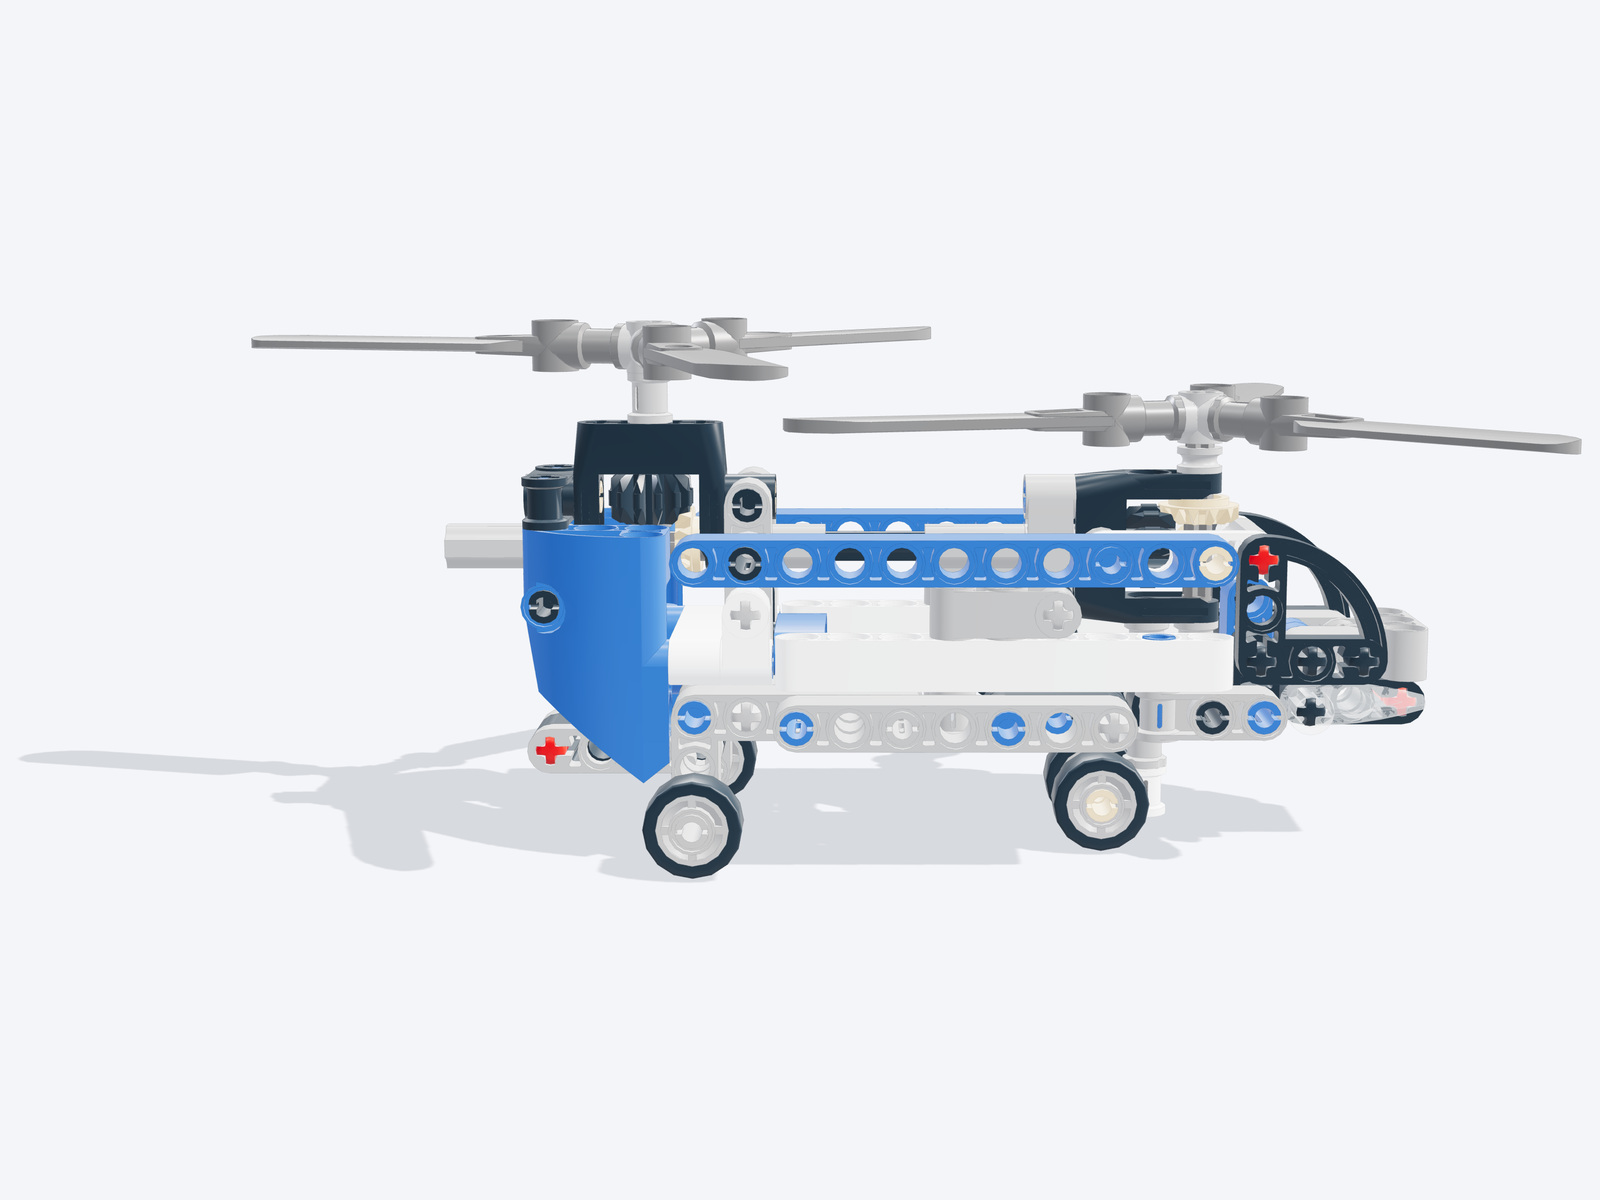
\includegraphics[width=.48\linewidth]{figures/ldraw/print/omr-42020-front.jpg}\\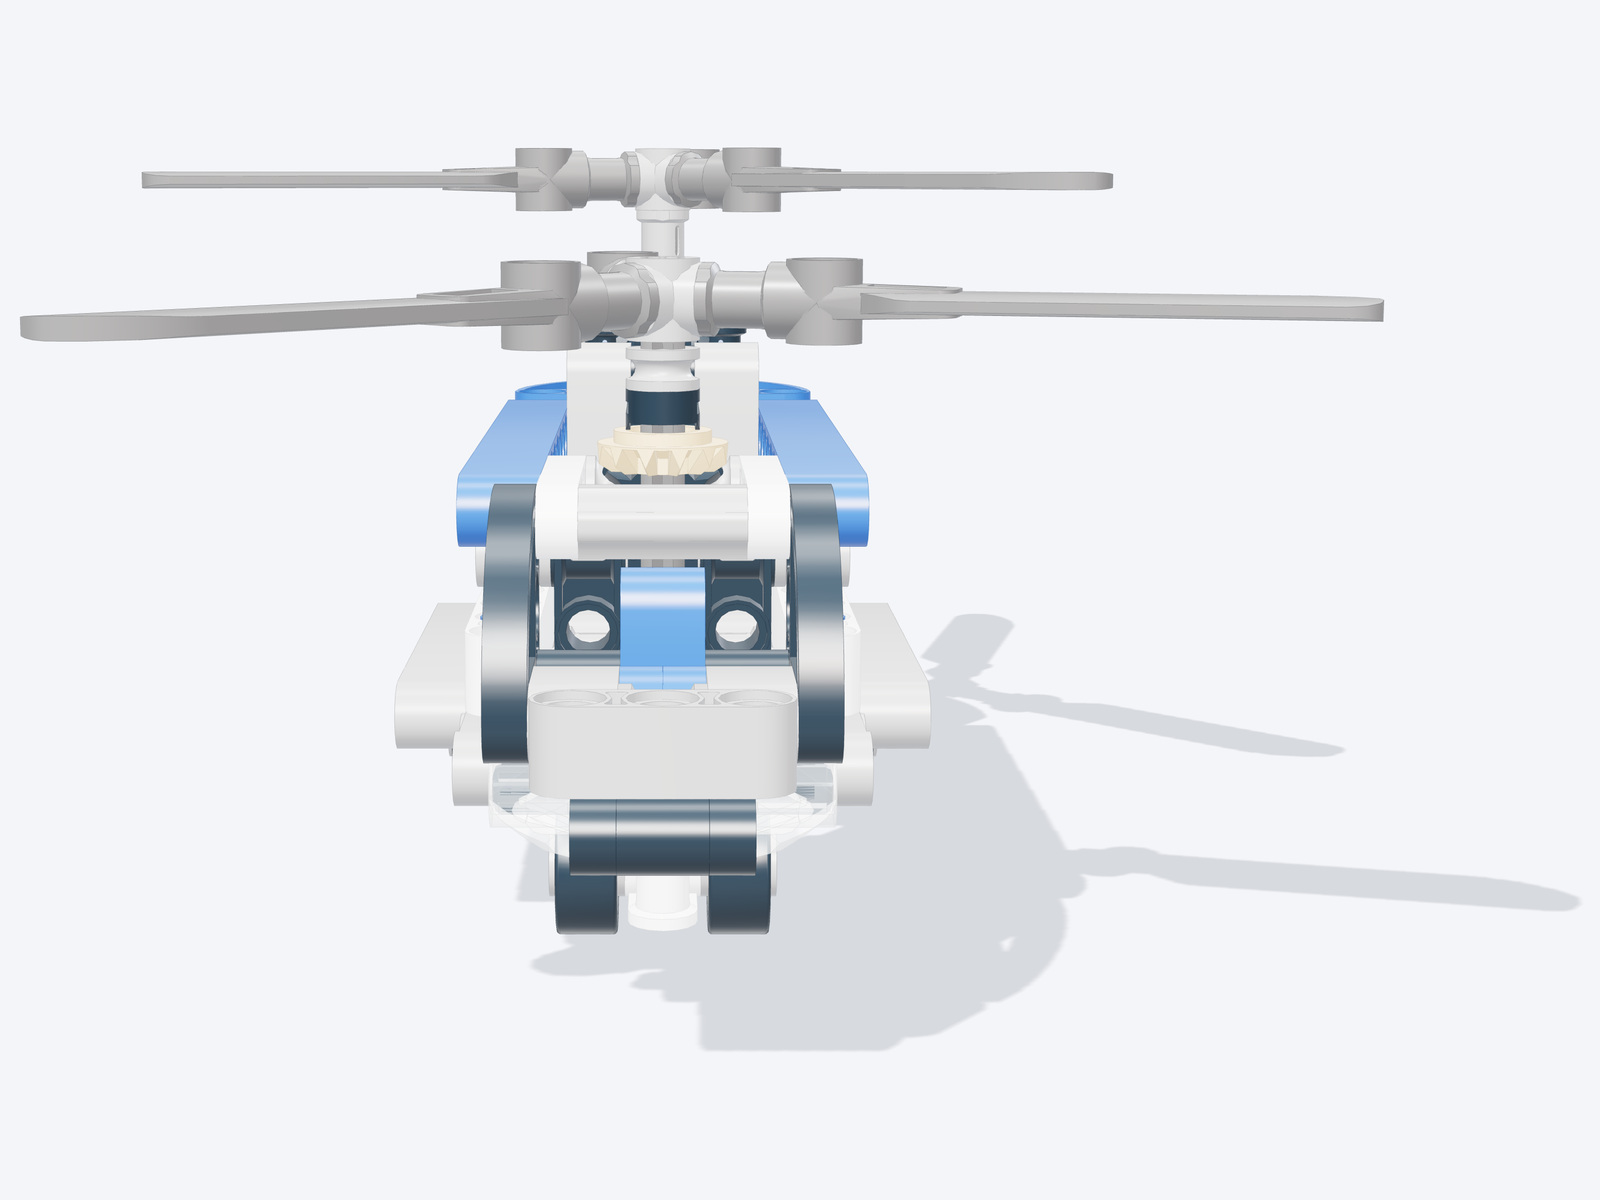
\includegraphics[width=.48\linewidth]{figures/ldraw/print/omr-42020-side.jpg}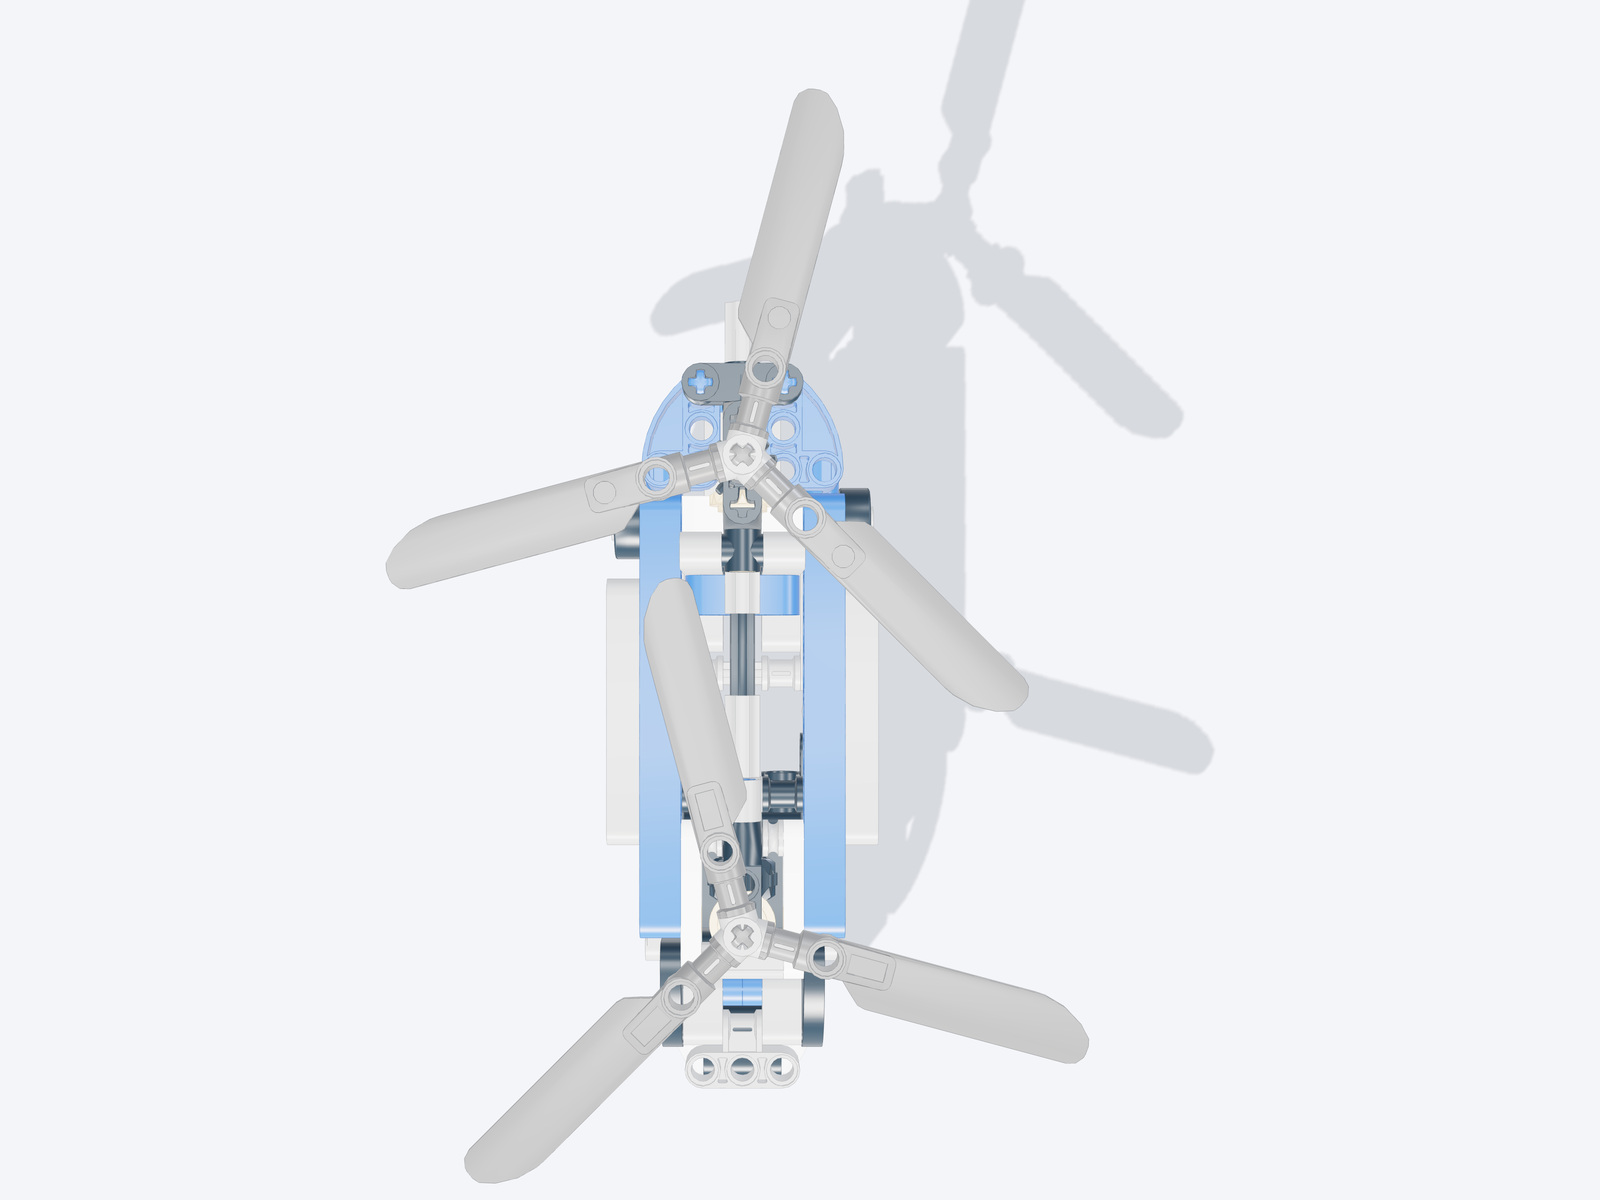
\includegraphics[width=.48\linewidth]{figures/ldraw/print/omr-42020-top.jpg}\end{center}
\paragraph{Attribution.}Faramond Florent [Makou]. CC BY 2.0.\par\noindent\url{https://library.ldraw.org/library/omr/42020-1.mpd}
\paragraph{Source lock.}\small\texttt{03ce9e9f6e5e8fe9b35ec612407be6ac}\\\texttt{51996d369a341775b5ae80b45d7017a2}\normalsize
\paragraph{Evidence coverage.}Connector definitions cover 100.00\% of instances. The audit reports 1 recognized-graph components and 0 intersection candidates without a recognized mating pair. 0 instances have no connector definition. These counts do not certify physical defects or gravitational stability.
\paragraph{Instructions.}No author STEP replay or source-order question is provided.
\clearpage\subsection{Numbered visual input and complete question index}
Only relevant numbers are shown. The website can isolate any instance; public visual tasks provide their own numbered images. The following entries give every English prompt, all choice options, compact public evidence and the reference output. Raw repeated connector records and full action fact sets remain in the versioned JSON.
\begin{center}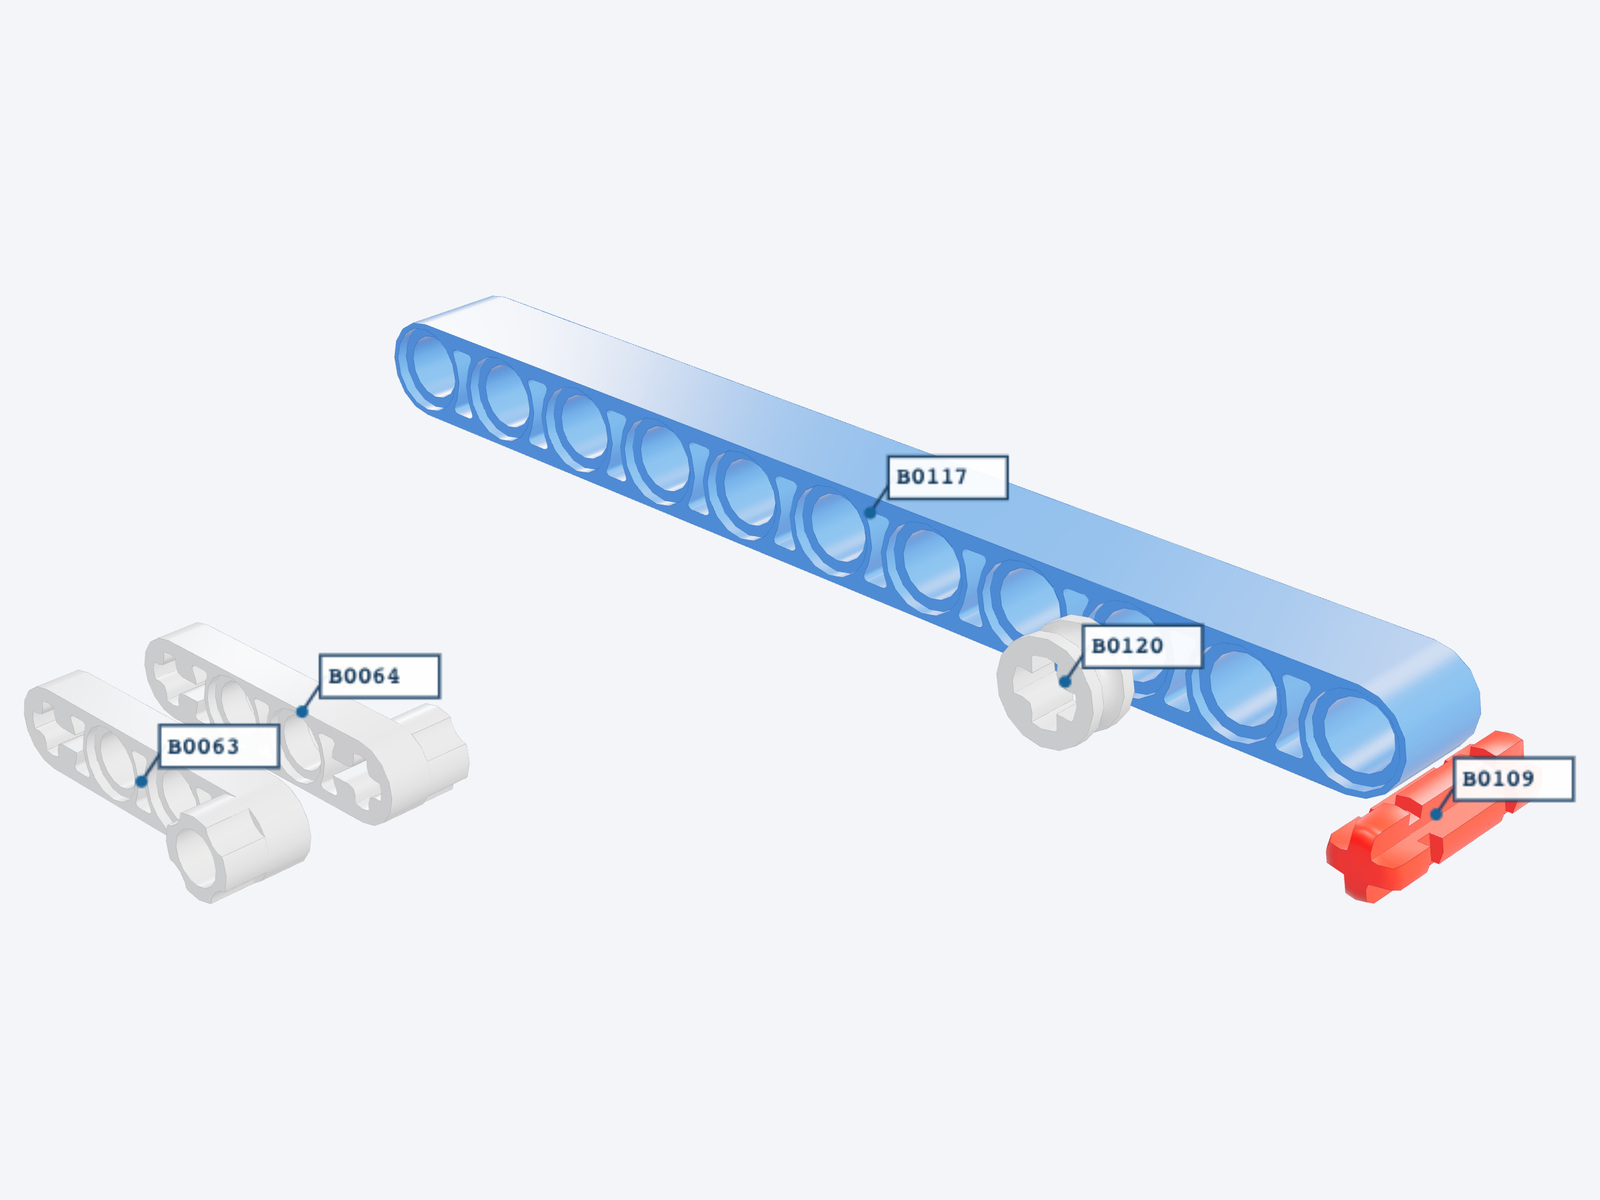
\includegraphics[width=.55\linewidth]{figures/ldraw/print/omr-42020-numbered.jpg}\end{center}
\begin{enumerate}
\item \textbf{color-1}. Identify the original color of B0064; numbered isolation is allowed.\par {\small \textit{Input:} Numbered visual input; source attributes are withheld from the model. \par\textit{Options:} A: Dark Bluish Grey; B: Red; C: Black; D: Light Bluish Grey. \par\textit{Reference output:} D.}
\item \textbf{shape-match-1}. Ignoring color and pose, which numbered instance has the same LDraw part type as B0064?\par {\small \textit{Input:} Numbered visual input; source attributes are withheld from the model. \par\textit{Options:} A: B0117; B: B0063; C: B0120; D: B0109. \par\textit{Reference output:} B.}
\item \textbf{distance-1}. Using the supplied geometry bounding-box centers, which candidate is nearest to B0064?\par {\small \textit{Input:} Centers (mm): B0064 = (16, -40, -20); B0053 = (32, -48, -8); B0107 = (22, -16, 88); B0051 = (-3.8, -23.2, -23.800047). \par\textit{Options:} A: B0051; B: B0107; C: B0053. \par\textit{Reference output:} C.}
\item \textbf{color-2}. Identify the original color of B0030; numbered isolation is allowed.\par {\small \textit{Input:} Numbered visual input; source attributes are withheld from the model. \par\textit{Options:} A: Light Bluish Grey; B: Red; C: White; D: Dark Bluish Grey. \par\textit{Reference output:} A.}
\item \textbf{distance-2}. Using the supplied geometry bounding-box centers, which candidate is nearest to B0030?\par {\small \textit{Input:} Centers (mm): B0030 = (8, -32, 24); B0132 = (0, -24, 92); B0052 = (8, -16, -32); B0017 = (24, -32, 8). \par\textit{Options:} A: B0132; B: B0052; C: B0017. \par\textit{Reference output:} C.}
\item \textbf{interface-1}. Classify the supplied connector record for B0004 and B0005. This does not certify load capacity.\par {\small \textit{Input:} Record: family = axle; connector indices = 0, 0. \par\textit{Options:} A: ball; B: fixed; C: hinge; D: axle. \par\textit{Reference output:} D.}
\item \textbf{interface-2}. Classify the supplied connector record for B0053 and B0059. This does not certify load capacity.\par {\small \textit{Input:} Record: family = fixed; connector indices = 1, 0. \par\textit{Options:} A: hinge; B: ball; C: fixed; D: axle. \par\textit{Reference output:} C.}
\item \textbf{neighbors-1}. Select every candidate directly adjacent to B0007 in the supplied connector graph.\par {\small \textit{Input:} Unique undirected pairs: B0007 / B0012; B0007 / B0035. \par\textit{Options:} A: B0086; B: B0023; C: B0035; D: B0012. \par\textit{Reference output:} C, D.}
\item \textbf{graph-removal-1}. Delete B0007 and its incident edges from this local graph. How many connected components remain? Do not infer physical extractability.\par {\small \textit{Input:} Nodes: B0007, B0035, B0012, B0086, B0023. Unique undirected pairs: B0007 / B0012; B0007 / B0035. \par\textit{Options:} A: 4; B: 3; C: 6; D: 5. \par\textit{Reference output:} A.}
\item \textbf{neighbors-2}. Select every candidate directly adjacent to B0079 in the supplied connector graph.\par {\small \textit{Input:} Unique undirected pairs: B0075 / B0079; B0079 / B0081. \par\textit{Options:} A: B0059; B: B0081; C: B0113; D: B0075. \par\textit{Reference output:} B, D.}
\item \textbf{graph-removal-2}. Delete B0079 and its incident edges from this local graph. How many connected components remain? Do not infer physical extractability.\par {\small \textit{Input:} Nodes: B0079, B0075, B0081, B0059, B0113. Unique undirected pairs: B0075 / B0079; B0079 / B0081. \par\textit{Options:} A: 5; B: 6; C: 3; D: 4. \par\textit{Reference output:} D.}
\item \textbf{evidence-limit-1}. Only source geometry, connector matching and mesh intersection audits are available. Without mass, friction, material or dynamic tests, is gravitational stability established?\par {\small \textit{Input:} Available evidence: Original CAD; Connector inference; Inset-mesh intersection candidates. \par\textit{Options:} A: Not established by this evidence; B: Established. \par\textit{Reference output:} A.}
\item \textbf{restore-instance-1}. The display copy hides B0064. Restore only that numbered instance, preserving all other instances and source poses.\par {\small \textit{Input:} Target: B0064. Action budget: 1. All other instances initially remain visible. \par\textit{Reference output:} restore-B0064.}
\item \textbf{restore-instance-2}. The display copy hides B0030. Restore only that numbered instance, preserving all other instances and source poses.\par {\small \textit{Input:} Target: B0030. Action budget: 1. All other instances initially remain visible. \par\textit{Reference output:} restore-B0030.}
\end{enumerate}
\clearpage
\section{10036: Pizza To Go}
166 source instances; 20 tasks; D2 scale band.

\par\noindent Perspective, front, side and top views follow in reading order. Original source transforms are preserved.
\begin{center}
\includegraphics[width=.48\linewidth]{figures/ldraw/print/10036-iso.jpg}
\includegraphics[width=.48\linewidth]{figures/ldraw/print/10036-front.jpg}\\
\includegraphics[width=.48\linewidth]{figures/ldraw/print/10036-side.jpg}
\includegraphics[width=.48\linewidth]{figures/ldraw/print/10036-top.jpg}\end{center}
\paragraph{Attribution.}Robert Paciorek [bercik]. CC BY 2.0.\par\noindent\url{https://library.ldraw.org/omr/sets/658}
\paragraph{Source lock.}\small\texttt{bb9eafb3fc283a4b3b28eef58d6f9208}\\\texttt{528ee3d9b3debe4a7db8bbadc85f63f8}\normalsize
\paragraph{Evidence coverage.}Connector definitions cover 100.00\% of instances. The audit reports 9 recognized-graph components and 3 intersection candidates without a recognized mating pair. 0 instances have no connector definition. These counts do not certify physical defects or gravitational stability.
\paragraph{Instructions.}29 expanded author steps.
\clearpage\subsection{Numbered visual input and complete question index}
Only relevant numbers are shown. The website can isolate any instance; public visual tasks provide their own numbered images. The following entries give every English prompt, all choice options, compact public evidence and the reference output. Raw repeated connector records and full action fact sets remain in the versioned JSON.
\begin{center}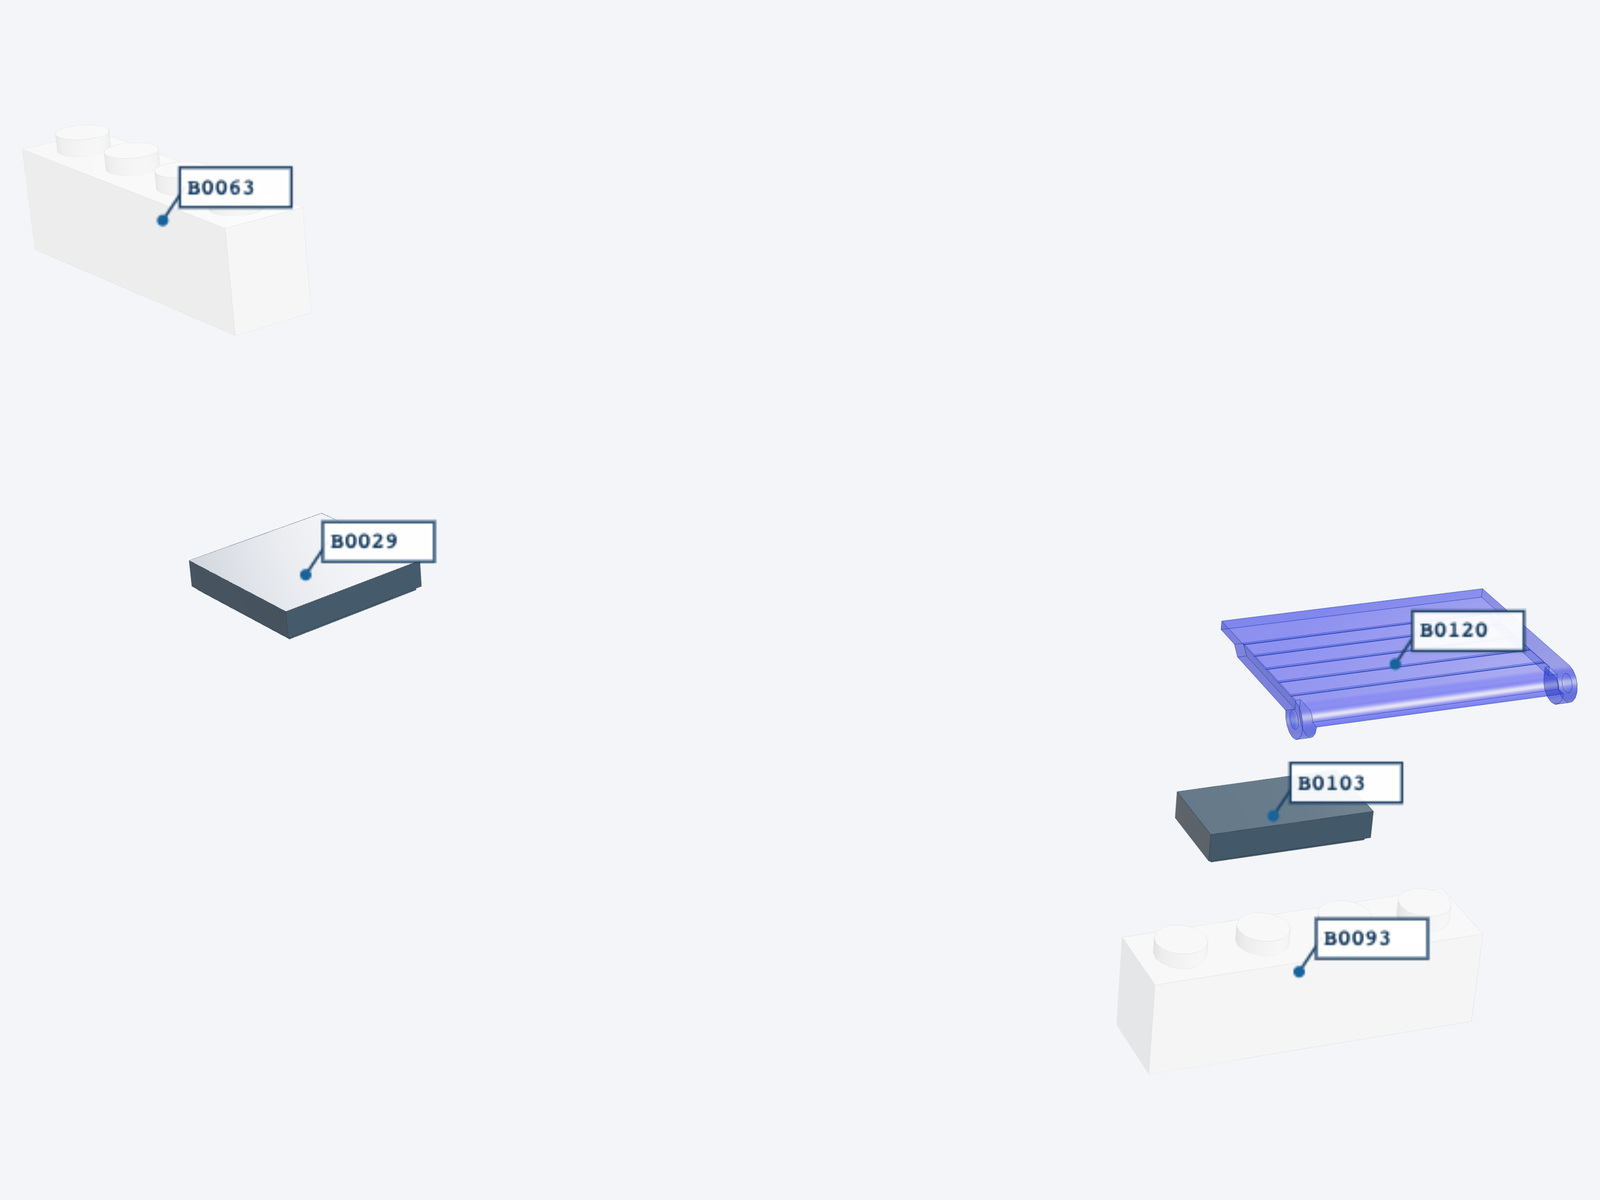
\includegraphics[width=.55\linewidth]{figures/ldraw/print/10036-numbered.jpg}\end{center}
\begin{enumerate}
\item \textbf{color-1}. Identify the original color of B0063; numbered isolation is allowed.\par {\small \textit{Input:} Numbered visual input; source attributes are withheld from the model. \par\textit{Options:} A: Dark Grey; B: White; C: Trans Light Blue; D: Brown. \par\textit{Reference output:} B.}
\item \textbf{shape-match-1}. Ignoring color and pose, which numbered instance has the same LDraw part type as B0063?\par {\small \textit{Input:} Numbered visual input; source attributes are withheld from the model. \par\textit{Options:} A: B0029; B: B0093; C: B0103; D: B0120. \par\textit{Reference output:} B.}
\item \textbf{distance-1}. Using the supplied geometry bounding-box centers, which candidate is nearest to B0063?\par {\small \textit{Input:} Centers (mm): B0063 = (32, 66.4, -20); B0149 = (45.643616, 13.999961, 60.094864); B0142 = (-54.752249, 18.188798, 57.747503); B0018 = (56, 24.8, -32). \par\textit{Options:} A: B0142; B: B0018; C: B0149. \par\textit{Reference output:} B.}
\item \textbf{color-2}. Identify the original color of B0162; numbered isolation is allowed.\par {\small \textit{Input:} Numbered visual input; source attributes are withheld from the model. \par\textit{Options:} A: Red; B: Yellow; C: Dark Grey; D: Black. \par\textit{Reference output:} B.}
\item \textbf{shape-match-2}. Ignoring color and pose, which numbered instance has the same LDraw part type as B0162?\par {\small \textit{Input:} Numbered visual input; source attributes are withheld from the model. \par\textit{Options:} A: B0164; B: B0067; C: B0054; D: B0140. \par\textit{Reference output:} D.}
\item \textbf{distance-2}. Using the supplied geometry bounding-box centers, which candidate is nearest to B0162?\par {\small \textit{Input:} Centers (mm): B0162 = (-11.3066, 22.571561, 56.5872); B0091 = (83.576354, -2.4, 76.832951); B0054 = (-28, 56.8, -32); B0151 = (40.744899, 22.572178, 54.210612). \par\textit{Options:} A: B0151; B: B0091; C: B0054. \par\textit{Reference output:} A.}
\item \textbf{interface-1}. Classify the supplied connector record for B0147 and B0148. This does not certify load capacity.\par {\small \textit{Input:} Record: family = axle; connector indices = 2, 0. \par\textit{Options:} A: axle; B: fixed; C: hinge; D: ball. \par\textit{Reference output:} A.}
\item \textbf{interface-2}. Classify the supplied connector record for B0128 and B0127. This does not certify load capacity.\par {\small \textit{Input:} Record: family = fixed; connector indices = 2, 0. \par\textit{Options:} A: fixed; B: hinge; C: axle; D: ball. \par\textit{Reference output:} A.}
\item \textbf{interface-3}. Classify the supplied connector record for B0140 and B0137. This does not certify load capacity.\par {\small \textit{Input:} Record: family = hinge; connector indices = 0, 5. \par\textit{Options:} A: ball; B: hinge; C: axle; D: fixed. \par\textit{Reference output:} B.}
\item \textbf{interface-4}. Classify the supplied connector record for B0090 and B0094. This does not certify load capacity.\par {\small \textit{Input:} Record: family = stud; connector indices = 8, 3. \par\textit{Options:} A: hinge; B: axle; C: fixed; D: ball; E: stud. \par\textit{Reference output:} E.}
\item \textbf{neighbors-1}. Select every candidate directly adjacent to B0161 in the supplied connector graph.\par {\small \textit{Input:} Unique undirected pairs: B0159 / B0161; B0161 / B0163. \par\textit{Options:} A: B0163; B: B0159; C: B0081; D: B0023. \par\textit{Reference output:} A, B.}
\item \textbf{graph-removal-1}. Delete B0161 and its incident edges from this local graph. How many connected components remain? Do not infer physical extractability.\par {\small \textit{Input:} Nodes: B0161, B0159, B0163, B0023, B0081. Unique undirected pairs: B0159 / B0161; B0161 / B0163. \par\textit{Options:} A: 4; B: 6; C: 5; D: 3. \par\textit{Reference output:} A.}
\item \textbf{neighbors-2}. Select every candidate directly adjacent to B0111 in the supplied connector graph.\par {\small \textit{Input:} Unique undirected pairs: B0099 / B0101; B0099 / B0111; B0101 / B0111; B0111 / B0115. \par\textit{Options:} A: B0099; B: B0136; C: B0115; D: B0162; E: B0101. \par\textit{Reference output:} A, C, E.}
\item \textbf{graph-removal-2}. Delete B0111 and its incident edges from this local graph. How many connected components remain? Do not infer physical extractability.\par {\small \textit{Input:} Nodes: B0111, B0115, B0101, B0099, B0162, B0136. Unique undirected pairs: B0099 / B0101; B0099 / B0111; B0101 / B0111; B0111 / B0115. \par\textit{Options:} A: 5; B: 4; C: 3; D: 6. \par\textit{Reference output:} B.}
\item \textbf{evidence-limit-1}. Only source geometry, connector matching and mesh intersection audits are available. Without mass, friction, material or dynamic tests, is gravitational stability established?\par {\small \textit{Input:} Available evidence: Original CAD; Connector inference; Inset-mesh intersection candidates. \par\textit{Options:} A: Established; B: Not established by this evidence. \par\textit{Reference output:} B.}
\item \textbf{source-step-1}. At which expanded author step does B0016 first appear in the supplied source-step table? Source order is not a collision-free assembly proof.\par {\small \textit{Input:} Expanded author records: step 1: B0001; step 4: B0016. \par\textit{Options:} A: 4; B: 5; C: 3; D: 6. \par\textit{Reference output:} A.}
\item \textbf{source-step-2}. At which expanded author step does B0044 first appear in the supplied source-step table? Source order is not a collision-free assembly proof.\par {\small \textit{Input:} Expanded author records: step 1: B0001; step 9: B0044. \par\textit{Options:} A: 10; B: 8; C: 11; D: 9. \par\textit{Reference output:} D.}
\item \textbf{source-sequence-1}. Reveal the supplied source-step window in author order. Actions change visibility only, without simulating insertion trajectories.\par {\small \textit{Input:} Source window: step-1: B0001, B0002, B0003; step-2: B0004, B0005, B0006, B0007, B0008; step-3: B0009, B0010, B0011, B0012, B0013, B0014, B0015; step-4: B0016, B0017, B0018; step-5: B0019, B0020, B0021; step-6: B0022, B0023, B0024, B0025, B0026, B0027, B0028, B0029. Action budget: 6. \par\textit{Reference output:} step-1, step-2, step-3, step-4, step-5, step-6.}
\item \textbf{restore-instance-1}. The display copy hides B0063. Restore only that numbered instance, preserving all other instances and source poses.\par {\small \textit{Input:} Target: B0063. Action budget: 1. All other instances initially remain visible. \par\textit{Reference output:} restore-B0063.}
\item \textbf{restore-instance-2}. The display copy hides B0162. Restore only that numbered instance, preserving all other instances and source poses.\par {\small \textit{Input:} Target: B0162. Action budget: 1. All other instances initially remain visible. \par\textit{Reference output:} restore-B0162.}
\end{enumerate}
\clearpage
\section{10014: Caboose}
170 source instances; 16 tasks; D2 scale band.

\par\noindent Perspective, front, side and top views follow in reading order. Original source transforms are preserved.
\begin{center}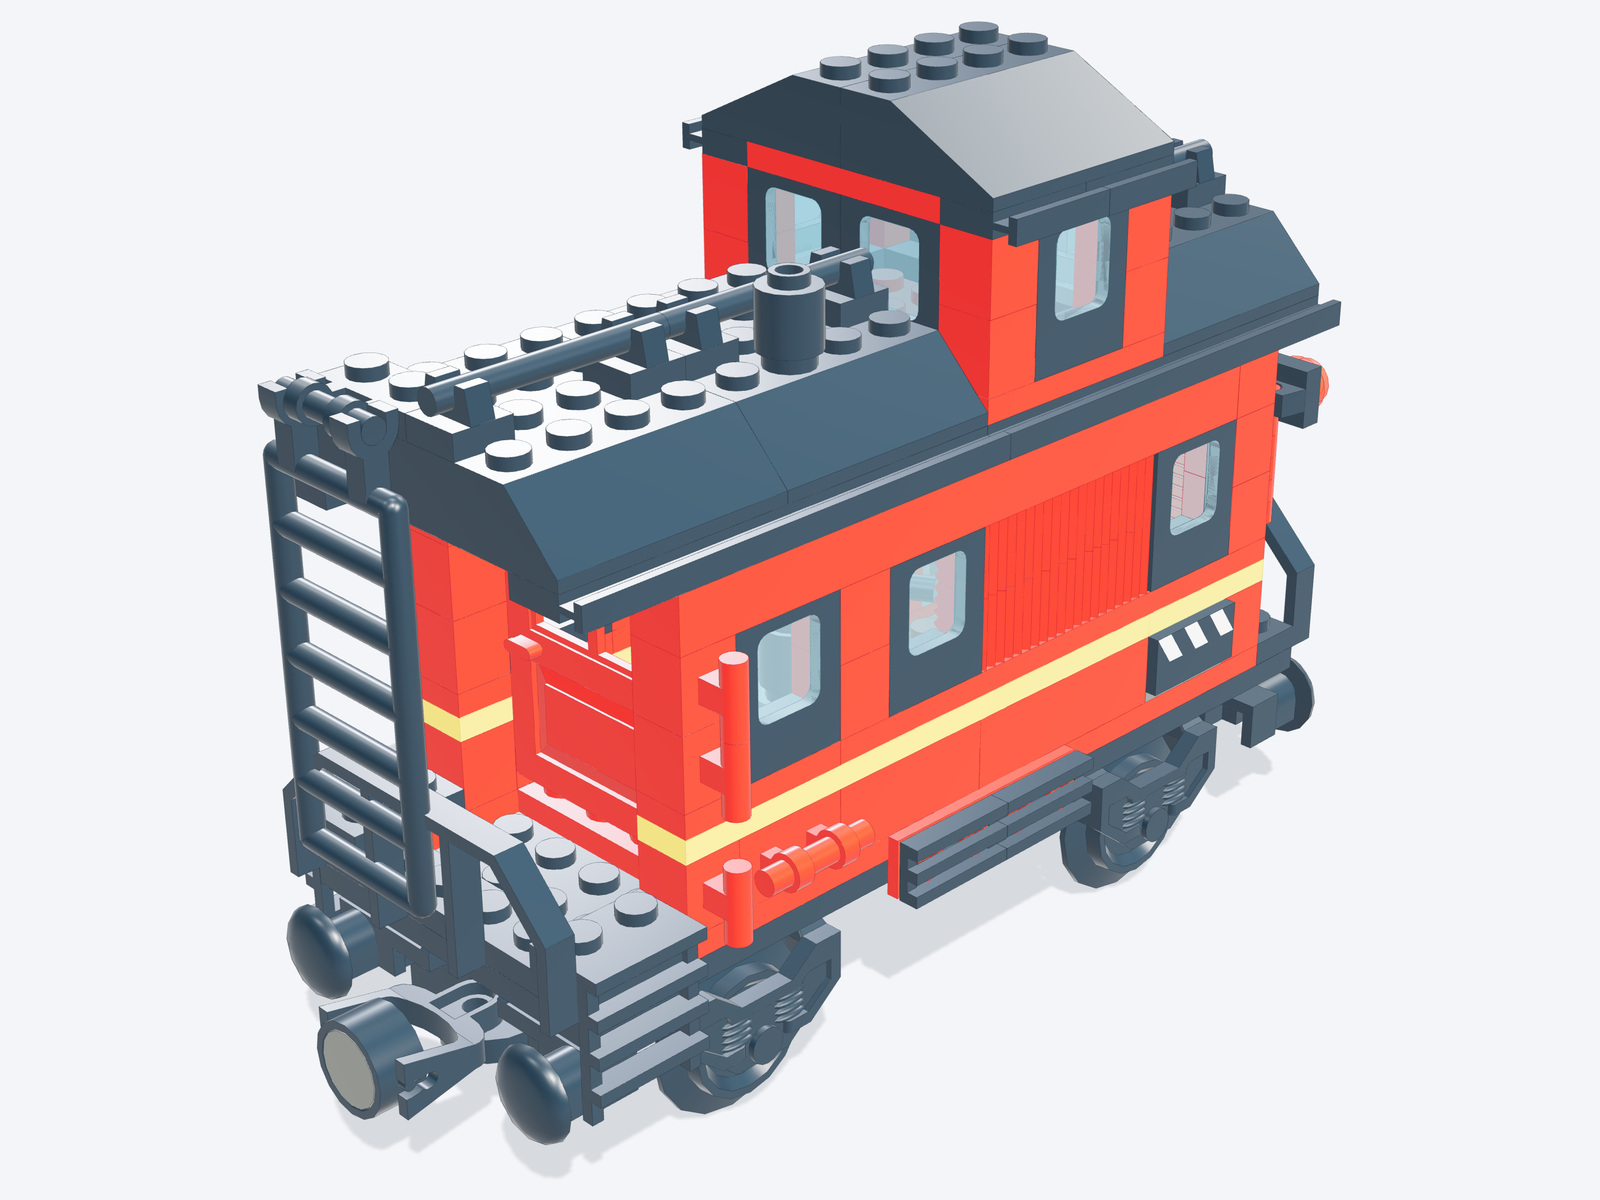
\includegraphics[width=.48\linewidth]{figures/ldraw/print/10014-iso.jpg}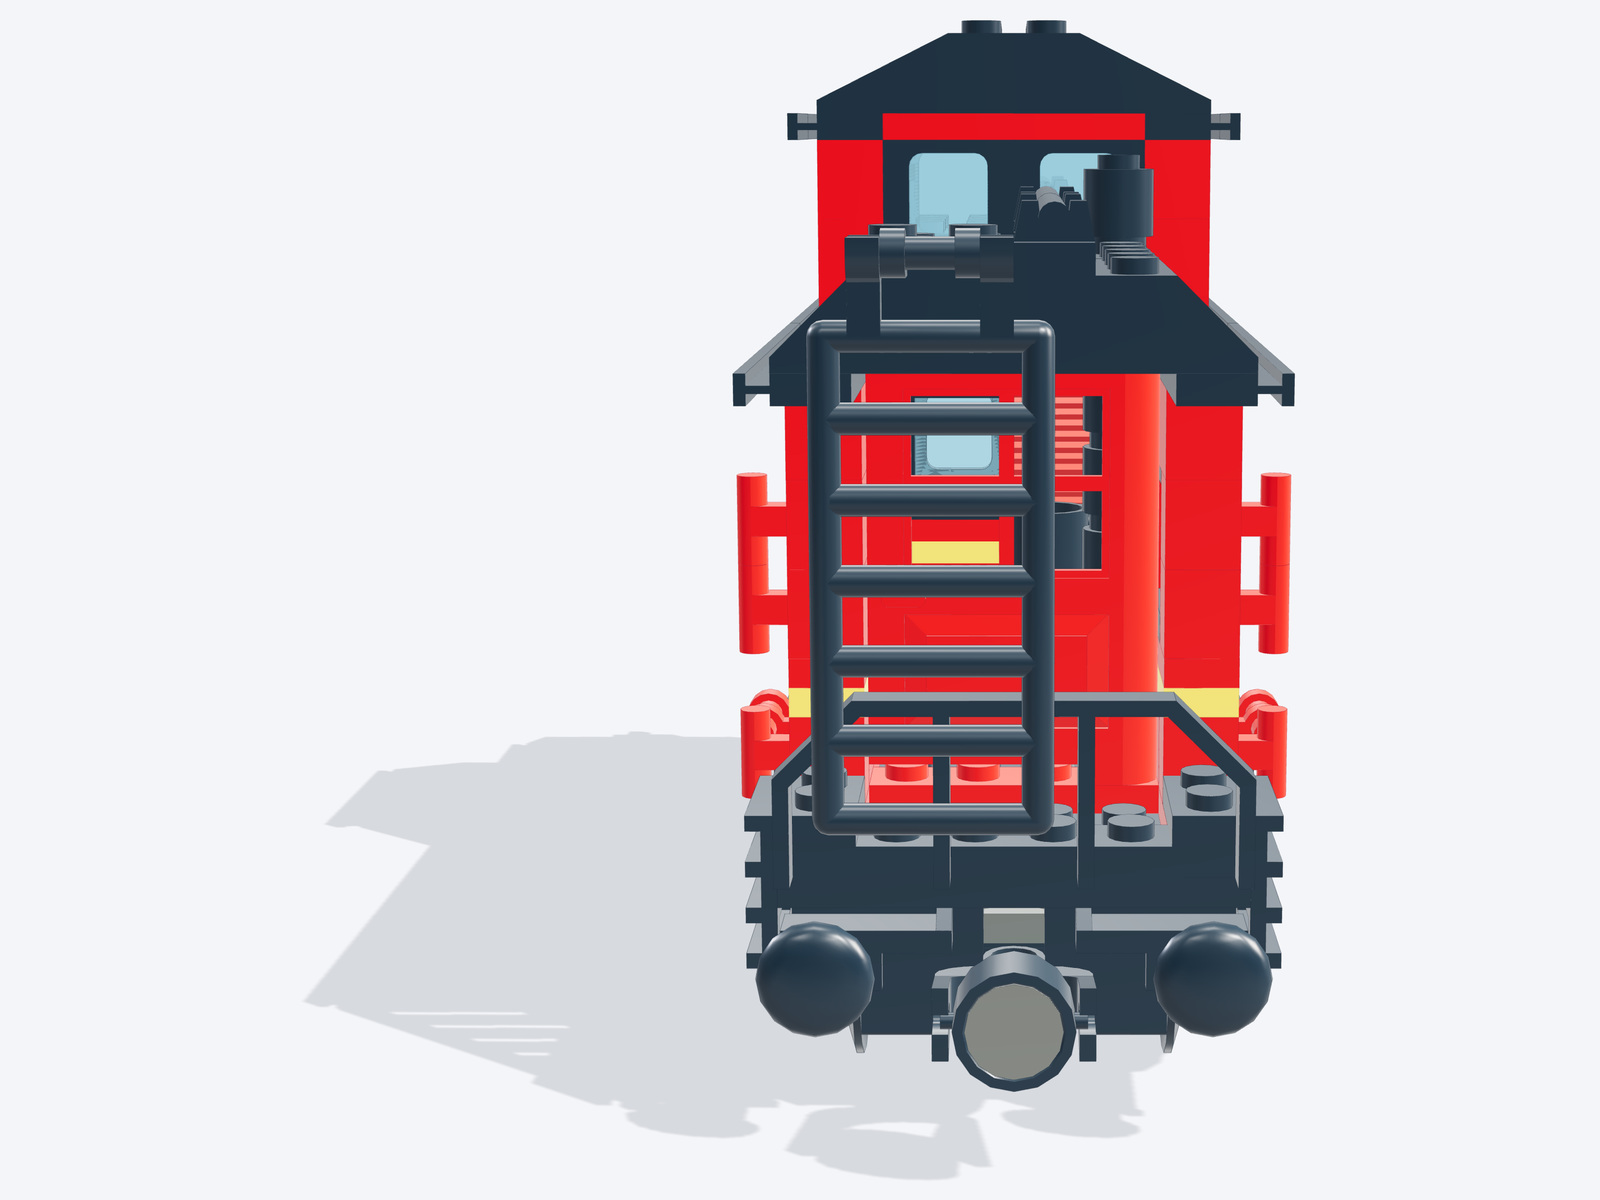
\includegraphics[width=.48\linewidth]{figures/ldraw/print/10014-front.jpg}\\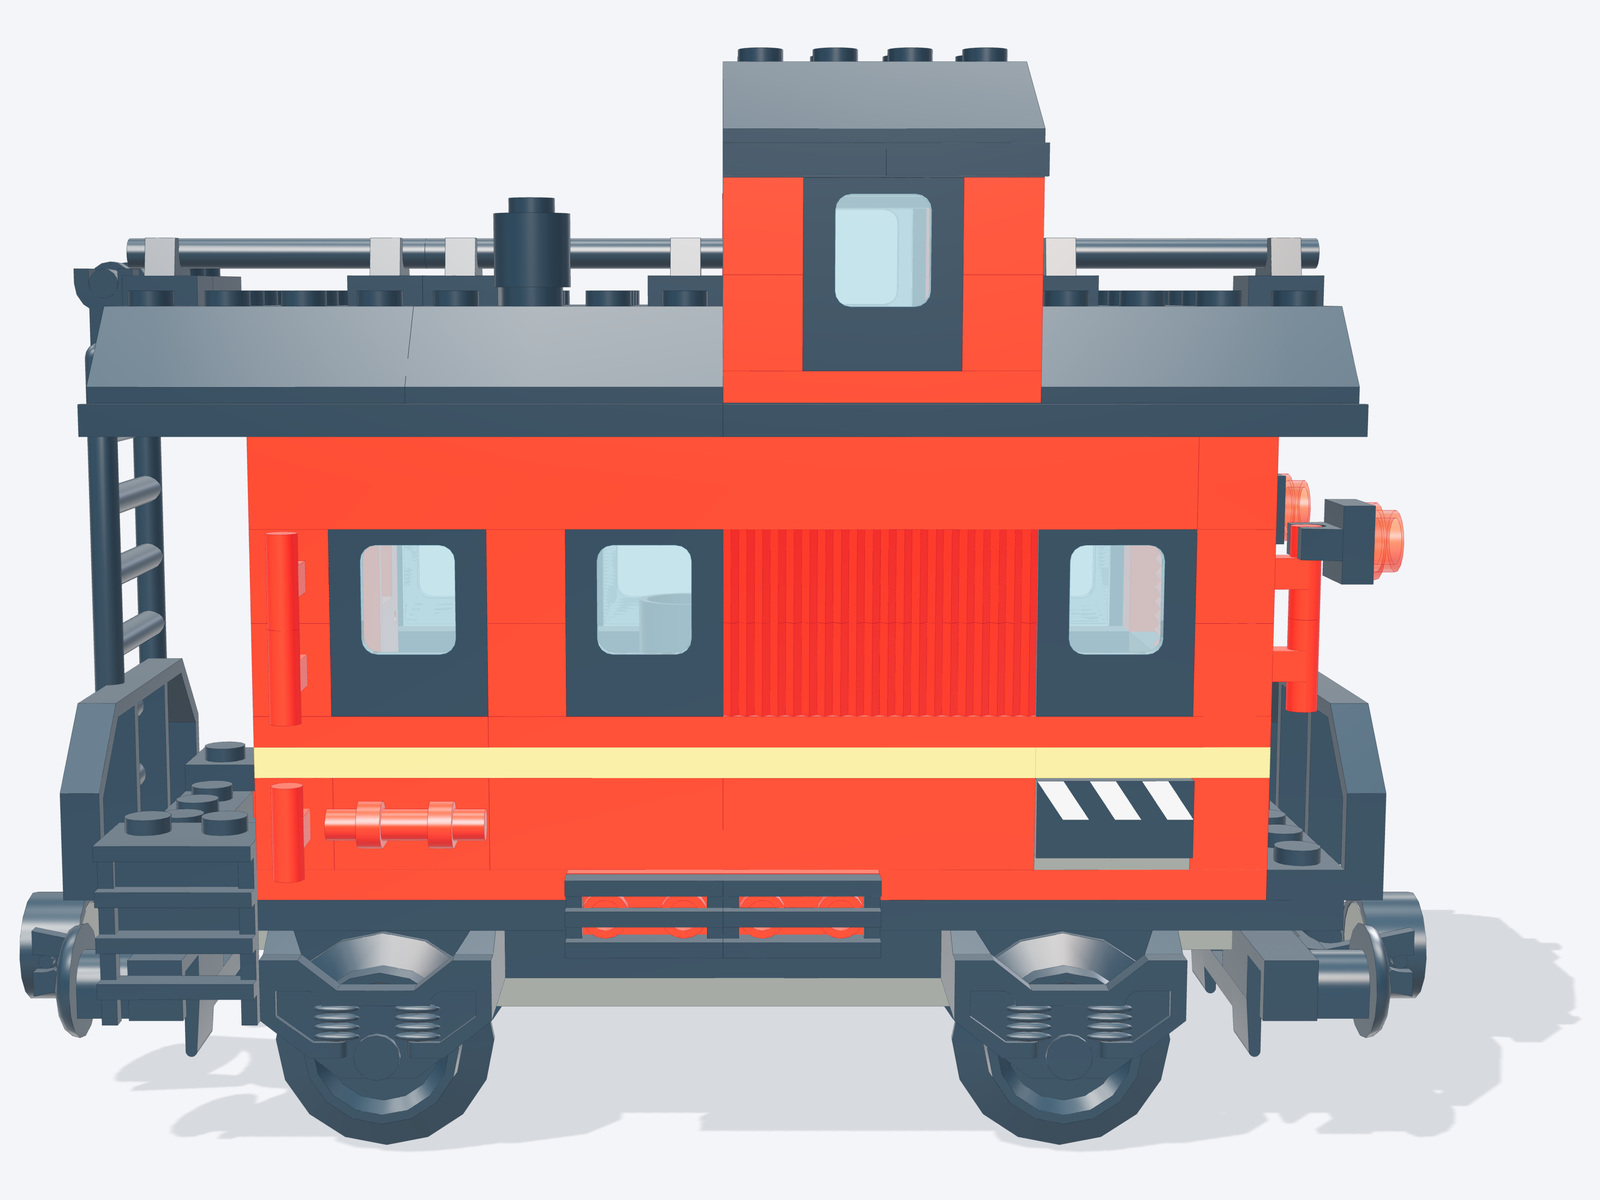
\includegraphics[width=.48\linewidth]{figures/ldraw/print/10014-side.jpg}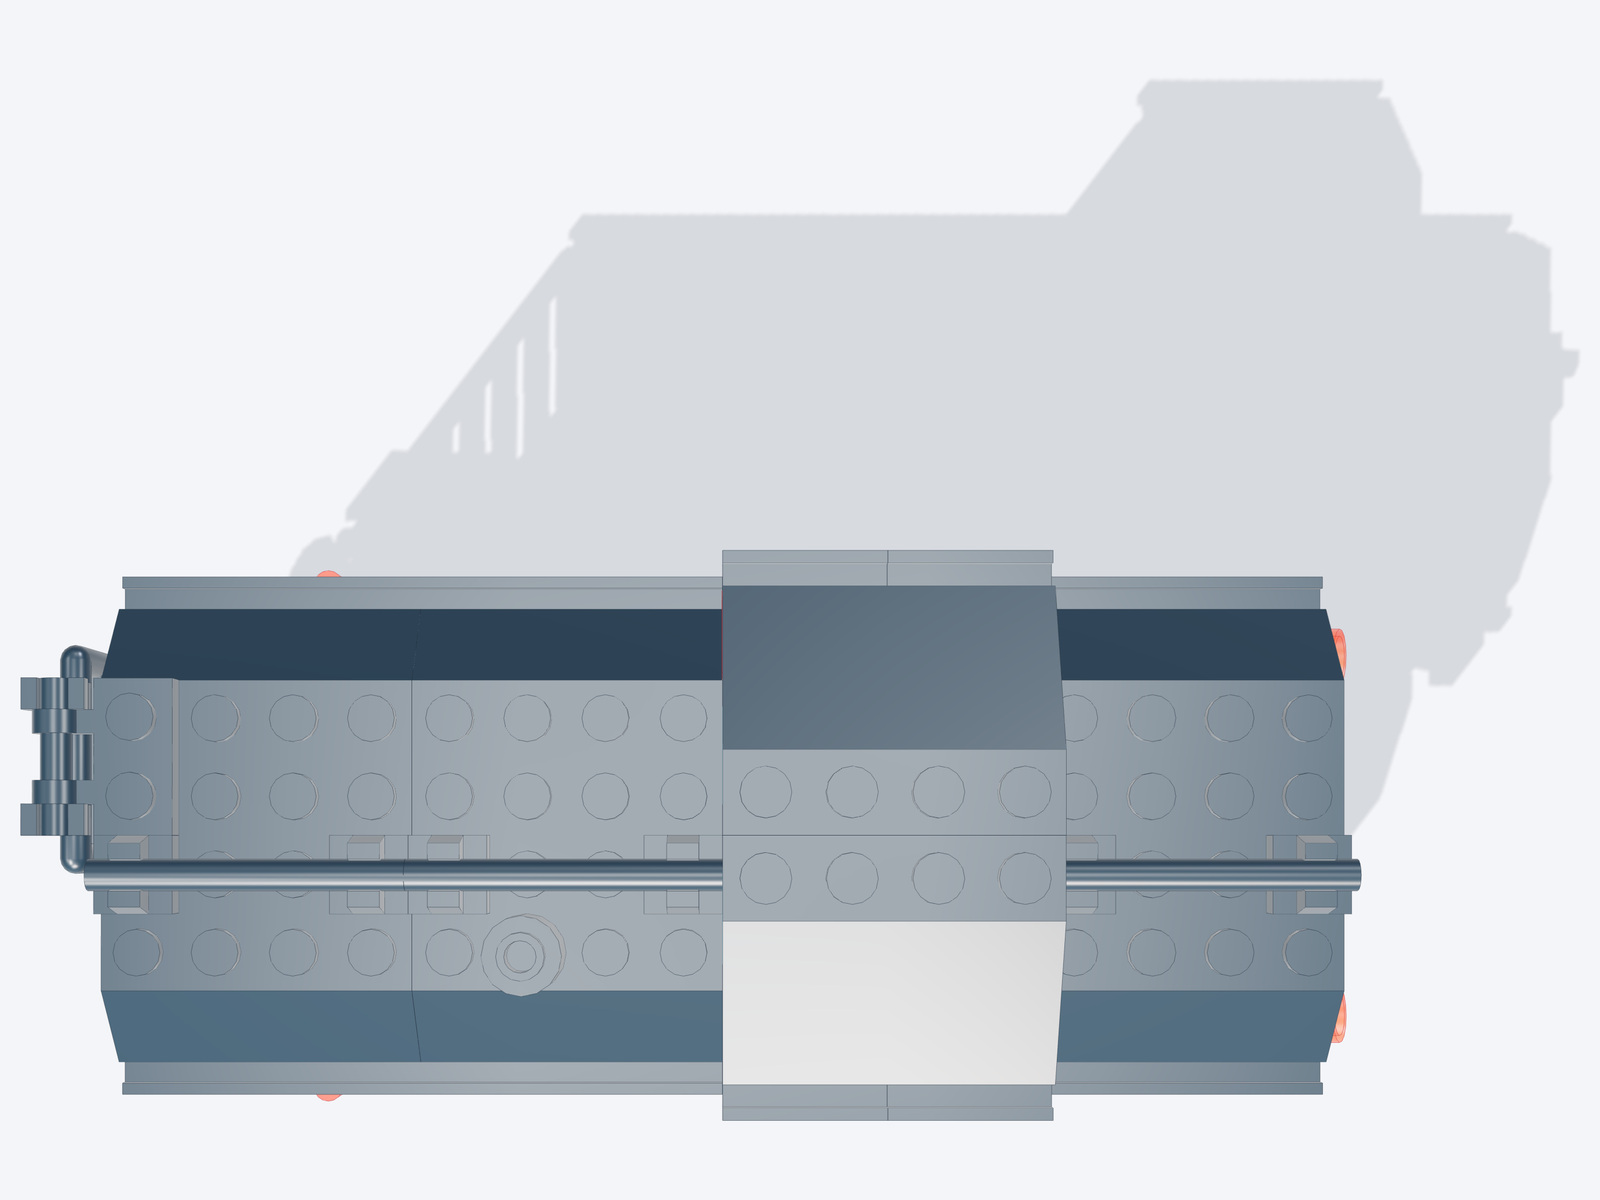
\includegraphics[width=.48\linewidth]{figures/ldraw/print/10014-top.jpg}\end{center}
\paragraph{Attribution.}TotalyWicked [TotalyWicked], OMR by Robert Paciorek [bercik]. CC BY 2.0.\par\noindent\url{https://library.ldraw.org/omr/sets/1415}
\paragraph{Source lock.}\small\texttt{f3aead9fe55512171565803f187f3f7a}\\\texttt{952fb70515983c39970cffd89431644d}\normalsize
\paragraph{Evidence coverage.}Connector definitions cover 91.18\% of instances. The audit reports 18 recognized-graph components and 1 intersection candidates without a recognized mating pair. 15 instances have no connector definition. These counts do not certify physical defects or gravitational stability.
\paragraph{Instructions.}No author STEP replay or source-order question is provided.
\clearpage\subsection{Numbered visual input and complete question index}
Only relevant numbers are shown. The website can isolate any instance; public visual tasks provide their own numbered images. The following entries give every English prompt, all choice options, compact public evidence and the reference output. Raw repeated connector records and full action fact sets remain in the versioned JSON.
\begin{center}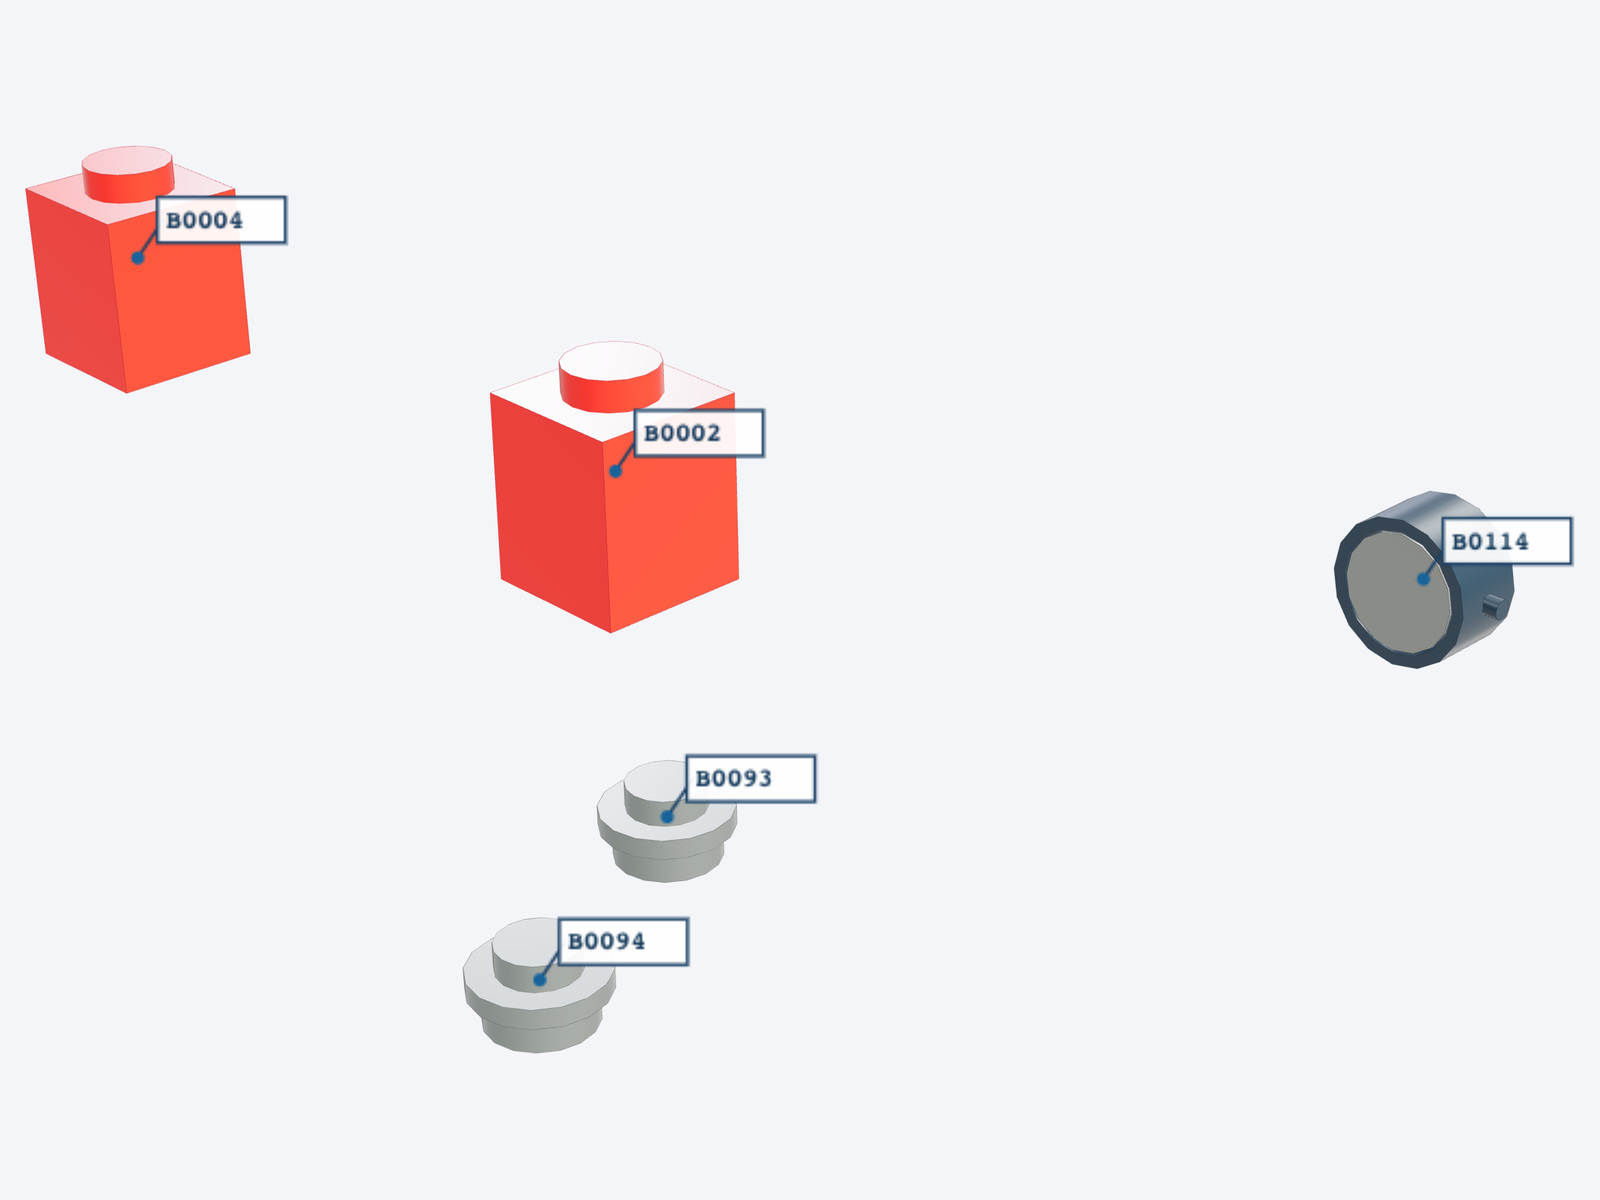
\includegraphics[width=.55\linewidth]{figures/ldraw/print/10014-numbered.jpg}\end{center}
\begin{enumerate}
\item \textbf{color-1}. Identify the original color of B0093; numbered isolation is allowed.\par {\small \textit{Input:} Numbered visual input; source attributes are withheld from the model. \par\textit{Options:} A: Light Grey; B: Dark Grey; C: Brown; D: Black. \par\textit{Reference output:} B.}
\item \textbf{shape-match-1}. Ignoring color and pose, which numbered instance has the same LDraw part type as B0093?\par {\small \textit{Input:} Numbered visual input; source attributes are withheld from the model. \par\textit{Options:} A: B0002; B: B0114; C: B0004; D: B0094. \par\textit{Reference output:} D.}
\item \textbf{distance-1}. Using the supplied geometry bounding-box centers, which candidate is nearest to B0093?\par {\small \textit{Input:} Centers (mm): B0093 = (-4, 2.4, 4); B0127 = (62, 9.6, 0); B0071 = (-12, 18.4, 8); B0004 = (-20, 34.4, -20). \par\textit{Options:} A: B0127; B: B0071; C: B0004. \par\textit{Reference output:} B.}
\item \textbf{color-2}. Identify the original color of B0139; numbered isolation is allowed.\par {\small \textit{Input:} Numbered visual input; source attributes are withheld from the model. \par\textit{Options:} A: Yellow; B: Trans Red; C: Black; D: Red. \par\textit{Reference output:} C.}
\item \textbf{shape-match-2}. Ignoring color and pose, which numbered instance has the same LDraw part type as B0139?\par {\small \textit{Input:} Numbered visual input; source attributes are withheld from the model. \par\textit{Options:} A: B0078; B: B0165; C: B0134; D: B0137. \par\textit{Reference output:} D.}
\item \textbf{distance-2}. Using the supplied geometry bounding-box centers, which candidate is nearest to B0139?\par {\small \textit{Input:} Centers (mm): B0139 = (-20, 44, 12); B0129 = (-8.008, -0.8, -27.2); B0056 = (54.8, 24.8, 20); B0141 = (24, 34.4, 20). \par\textit{Options:} A: B0056; B: B0141; C: B0129. \par\textit{Reference output:} B.}
\item \textbf{interface-1}. Classify the supplied connector record for B0021 and B0019. This does not certify load capacity.\par {\small \textit{Input:} Record: family = axle; connector indices = 0, 0. \par\textit{Options:} A: fixed; B: axle; C: hinge; D: ball. \par\textit{Reference output:} B.}
\item \textbf{interface-2}. Classify the supplied connector record for B0082 and B0067. This does not certify load capacity.\par {\small \textit{Input:} Record: family = stud; connector indices = 5, 9. \par\textit{Options:} A: stud; B: fixed; C: axle; D: hinge; E: ball. \par\textit{Reference output:} A.}
\item \textbf{neighbors-1}. Select every candidate directly adjacent to B0032 in the supplied connector graph.\par {\small \textit{Input:} Unique undirected pairs: B0015 / B0032; B0020 / B0032; B0021 / B0032; B0032 / B0163; B0032 / B0165. \par\textit{Options:} A: B0020; B: B0165; C: B0163; D: B0068; E: B0021; F: B0006; G: B0015. \par\textit{Reference output:} A, B, C, E, G.}
\item \textbf{graph-removal-1}. Delete B0032 and its incident edges from this local graph. How many connected components remain? Do not infer physical extractability.\par {\small \textit{Input:} Nodes: B0032, B0021, B0165, B0163, B0020, B0015, B0006, B0068. Unique undirected pairs: B0015 / B0032; B0020 / B0032; B0021 / B0032; B0032 / B0163; B0032 / B0165. \par\textit{Options:} A: 6; B: 9; C: 8; D: 7. \par\textit{Reference output:} D.}
\item \textbf{neighbors-2}. Select every candidate directly adjacent to B0024 in the supplied connector graph.\par {\small \textit{Input:} Unique undirected pairs: B0024 / B0025; B0024 / B0026; B0024 / B0029; B0024 / B0030. \par\textit{Options:} A: B0030; B: B0025; C: B0026; D: B0126; E: B0129; F: B0029. \par\textit{Reference output:} A, B, C, F.}
\item \textbf{graph-removal-2}. Delete B0024 and its incident edges from this local graph. How many connected components remain? Do not infer physical extractability.\par {\small \textit{Input:} Nodes: B0024, B0026, B0030, B0029, B0025, B0129, B0126. Unique undirected pairs: B0024 / B0025; B0024 / B0026; B0024 / B0029; B0024 / B0030. \par\textit{Options:} A: 8; B: 7; C: 5; D: 6. \par\textit{Reference output:} D.}
\item \textbf{coverage-1}. Which numbered instance lacks a connector definition in the coverage record, so this audit cannot establish that it is floating?\par {\small \textit{Input:} Definition coverage: B0033 = unsupported; B0093 = supported; B0139 = supported; B0074 = supported. \par\textit{Options:} A: B0033; B: B0093; C: B0074; D: B0139. \par\textit{Reference output:} A.}
\item \textbf{evidence-limit-1}. Only source geometry, connector matching and mesh intersection audits are available. Without mass, friction, material or dynamic tests, is gravitational stability established?\par {\small \textit{Input:} Available evidence: Original CAD; Connector inference; Inset-mesh intersection candidates. \par\textit{Options:} A: Not established by this evidence; B: Established. \par\textit{Reference output:} A.}
\item \textbf{restore-instance-1}. The display copy hides B0093. Restore only that numbered instance, preserving all other instances and source poses.\par {\small \textit{Input:} Target: B0093. Action budget: 1. All other instances initially remain visible. \par\textit{Reference output:} restore-B0093.}
\item \textbf{restore-instance-2}. The display copy hides B0139. Restore only that numbered instance, preserving all other instances and source poses.\par {\small \textit{Input:} Target: B0139. Action budget: 1. All other instances initially remain visible. \par\textit{Reference output:} restore-B0139.}
\end{enumerate}
\clearpage
\section{31031: Rainforest Animals}
215 source instances; 20 tasks; D2 scale band.

\par\noindent Perspective, front, side and top views follow in reading order. Original source transforms are preserved.
\begin{center}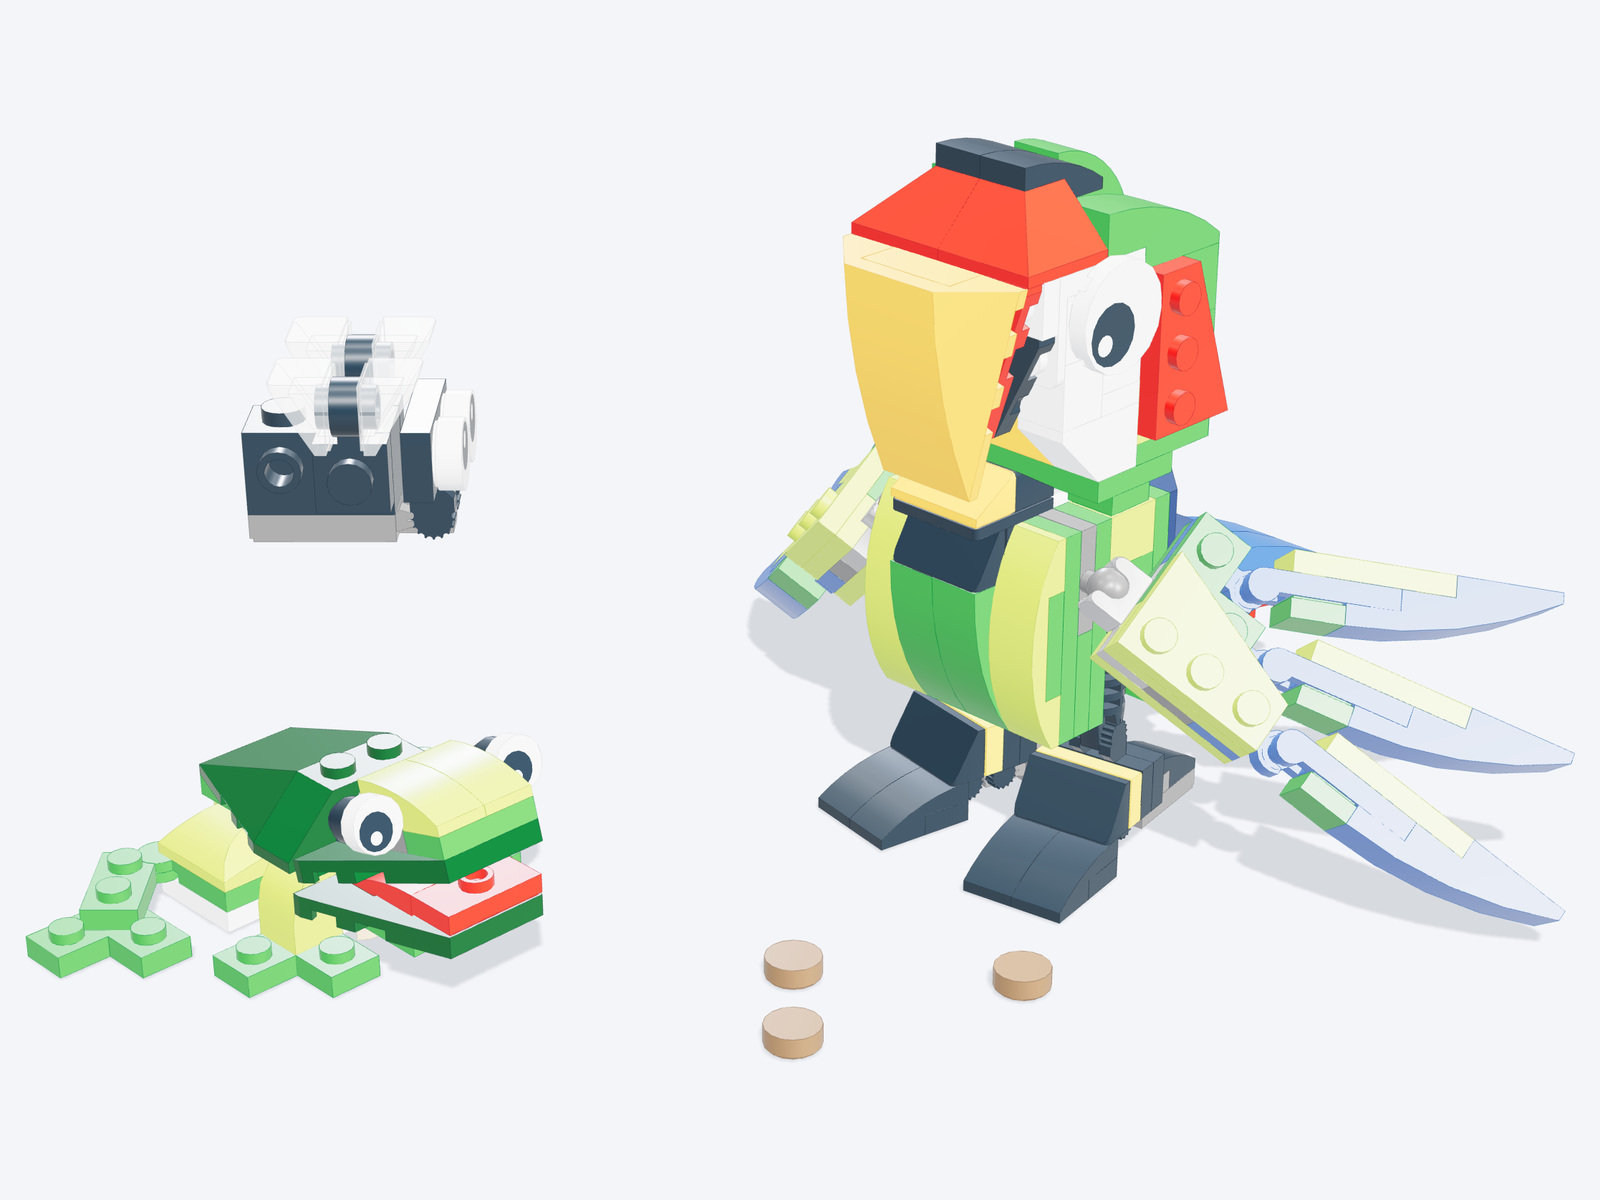
\includegraphics[width=.48\linewidth]{figures/ldraw/print/omr-31031-iso.jpg}
\includegraphics[width=.48\linewidth]{figures/ldraw/print/omr-31031-front.jpg}\\
\includegraphics[width=.48\linewidth]{figures/ldraw/print/omr-31031-side.jpg}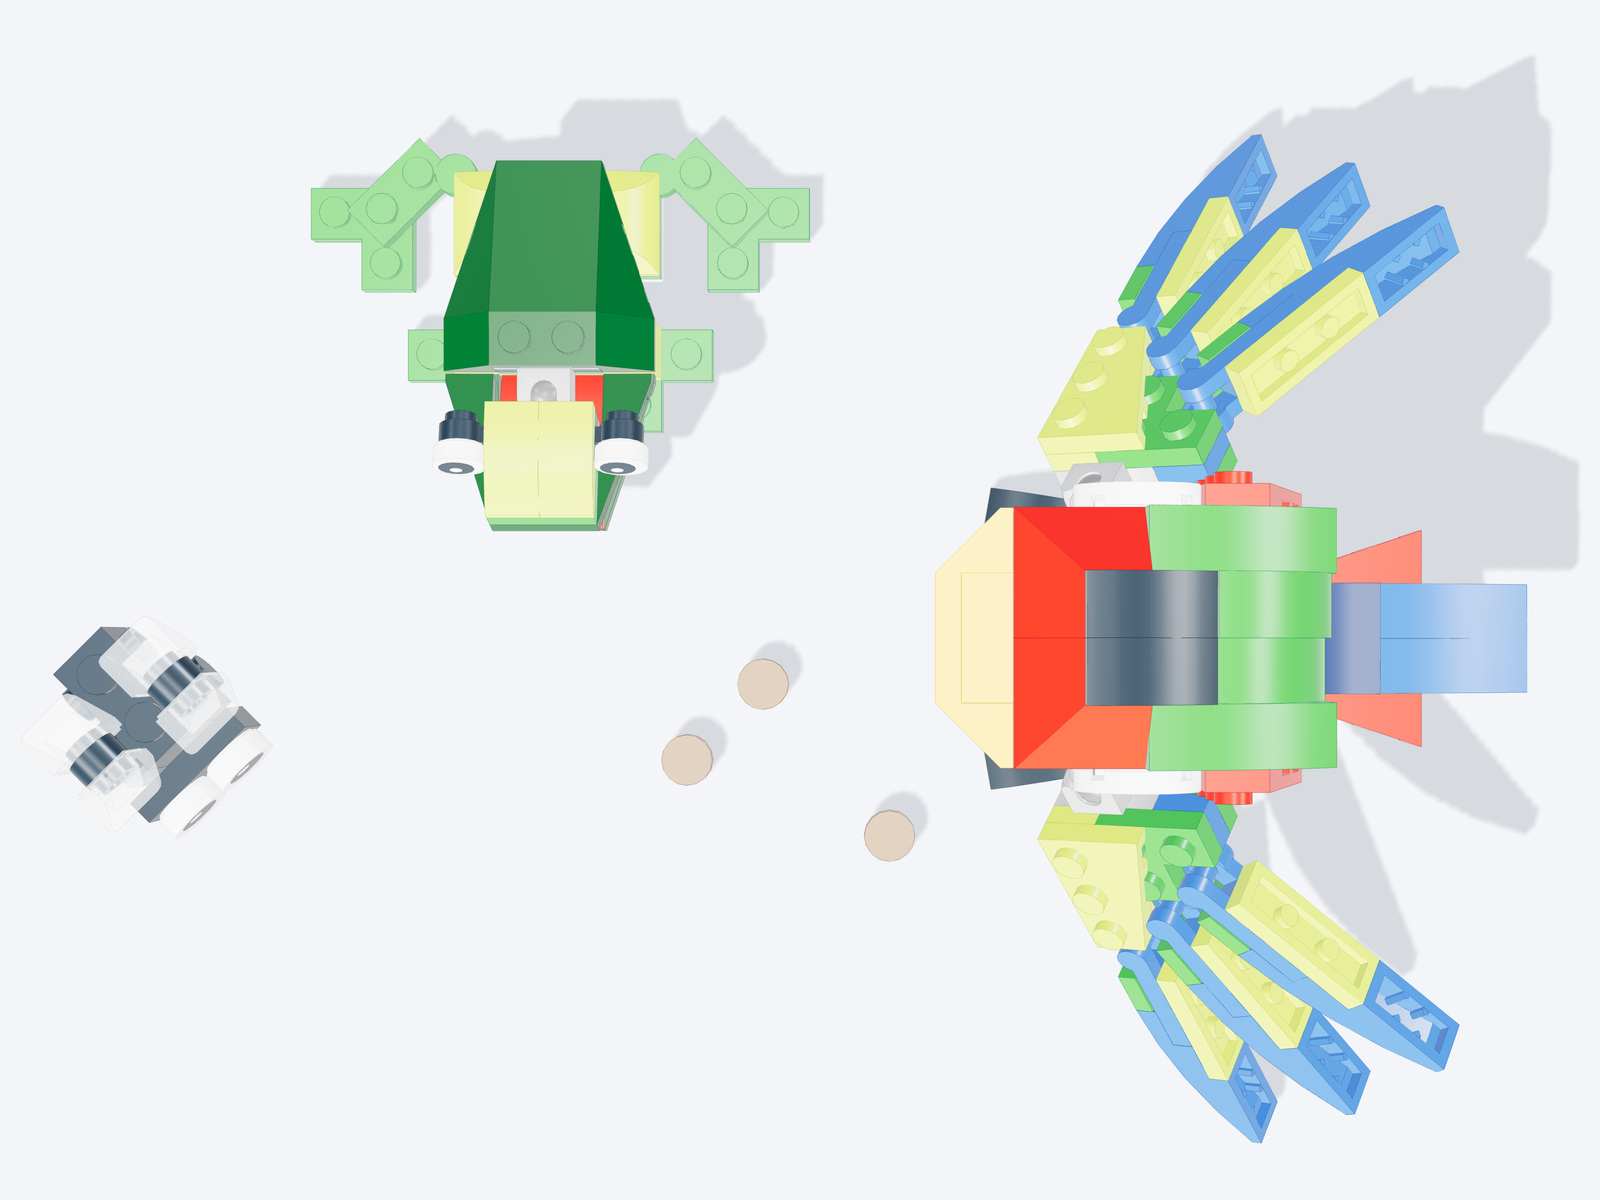
\includegraphics[width=.48\linewidth]{figures/ldraw/print/omr-31031-top.jpg}\end{center}
\paragraph{Attribution.}Marc Giraudet [Mad\_Marc]. CC BY 2.0.\par\noindent\url{https://library.ldraw.org/library/omr/31031-1.mpd}
\paragraph{Source lock.}\small\texttt{b5b87230d2fe147aa1135baee5d1604a}\\\texttt{283f1e586a228b27b351253af5565da7}\normalsize
\paragraph{Evidence coverage.}Connector definitions cover 100.00\% of instances. The audit reports 12 recognized-graph components and 7 intersection candidates without a recognized mating pair. 0 instances have no connector definition. These counts do not certify physical defects or gravitational stability.
\paragraph{Instructions.}130 expanded author steps.
\clearpage\subsection{Numbered visual input and complete question index}
Only relevant numbers are shown. The website can isolate any instance; public visual tasks provide their own numbered images. The following entries give every English prompt, all choice options, compact public evidence and the reference output. Raw repeated connector records and full action fact sets remain in the versioned JSON.
\begin{center}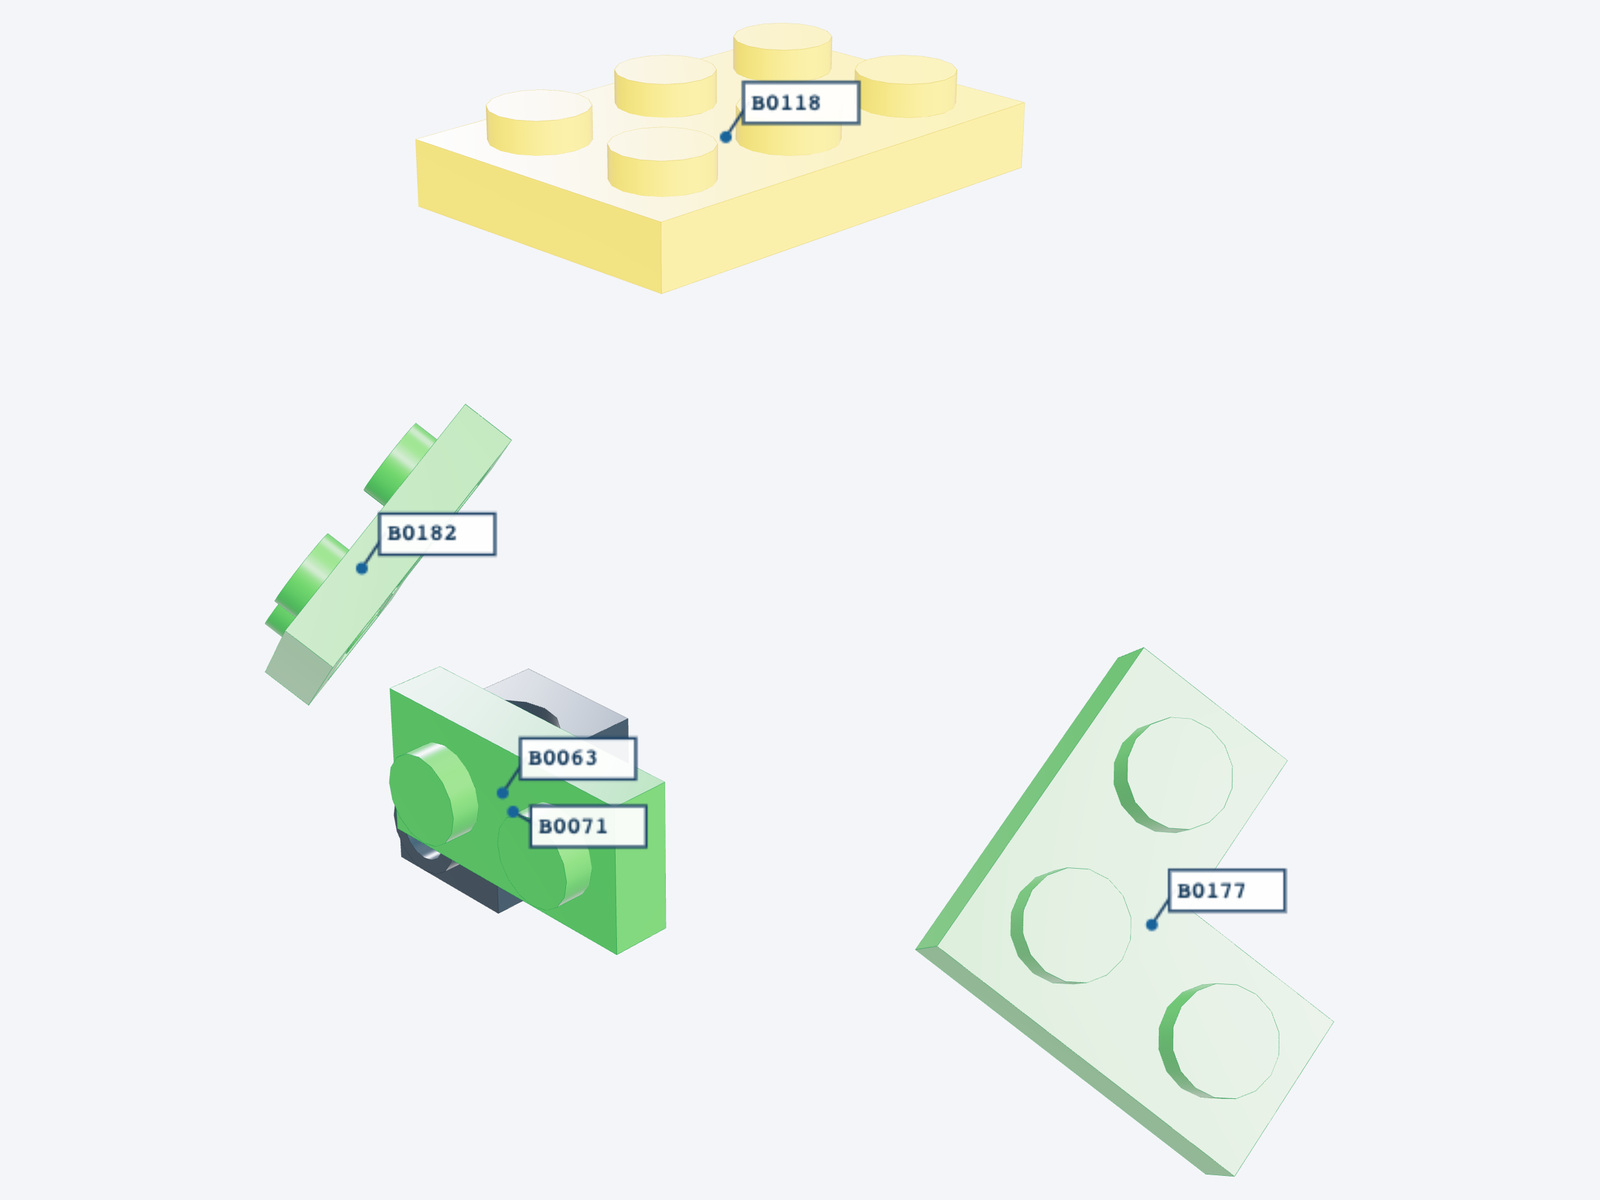
\includegraphics[width=.55\linewidth]{figures/ldraw/print/omr-31031-numbered.jpg}\end{center}
\begin{enumerate}
\item \textbf{color-1}. Identify the original color of B0182; numbered isolation is allowed.\par {\small \textit{Input:} Numbered visual input; source attributes are withheld from the model. \par\textit{Options:} A: Green; B: Blue; C: Trans Clear; D: Bright Light Orange. \par\textit{Reference output:} A.}
\item \textbf{shape-match-1}. Ignoring color and pose, which numbered instance has the same LDraw part type as B0182?\par {\small \textit{Input:} Numbered visual input; source attributes are withheld from the model. \par\textit{Options:} A: B0118; B: B0063; C: B0177; D: B0071. \par\textit{Reference output:} C.}
\item \textbf{distance-1}. Using the supplied geometry bounding-box centers, which candidate is nearest to B0182?\par {\small \textit{Input:} Centers (mm): B0182 = (11.8912, 42.1888, -13.4232); B0038 = (-80, 22.103829, -19.584571); B0096 = (-6.066, 3.200012, 2.0992); B0004 = (-115.958788, 106.4, 14.991612). \par\textit{Options:} A: B0038; B: B0004; C: B0096. \par\textit{Reference output:} C.}
\item \textbf{color-2}. Identify the original color of B0111; numbered isolation is allowed.\par {\small \textit{Input:} Numbered visual input; source attributes are withheld from the model. \par\textit{Options:} A: Lime; B: Green; C: Yellow; D: White. \par\textit{Reference output:} B.}
\item \textbf{shape-match-2}. Ignoring color and pose, which numbered instance has the same LDraw part type as B0111?\par {\small \textit{Input:} Numbered visual input; source attributes are withheld from the model. \par\textit{Options:} A: B0097; B: B0141; C: B0098; D: B0005. \par\textit{Reference output:} B.}
\item \textbf{distance-2}. Using the supplied geometry bounding-box centers, which candidate is nearest to B0111?\par {\small \textit{Input:} Centers (mm): B0111 = (14.4, 69.6, 12.8); B0142 = (14.4, 92.8, 8.8); B0094 = (1.3218, 2.4, -1.1448); B0149 = (2.4, 85.6, 30.4). \par\textit{Options:} A: B0094; B: B0149; C: B0142. \par\textit{Reference output:} C.}
\item \textbf{interface-1}. Classify the supplied connector record for B0049 and B0110. This does not certify load capacity.\par {\small \textit{Input:} Record: family = axle; connector indices = 1, 0. \par\textit{Options:} A: fixed; B: axle; C: hinge; D: ball. \par\textit{Reference output:} B.}
\item \textbf{interface-2}. Classify the supplied connector record for B0038 and B0035. This does not certify load capacity.\par {\small \textit{Input:} Record: family = ball; connector indices = 3, 3. \par\textit{Options:} A: hinge; B: fixed; C: axle; D: ball. \par\textit{Reference output:} D.}
\item \textbf{interface-3}. Classify the supplied connector record for B0015 and B0016. This does not certify load capacity.\par {\small \textit{Input:} Record: family = hinge; connector indices = 1, 2. \par\textit{Options:} A: hinge; B: ball; C: fixed; D: axle. \par\textit{Reference output:} A.}
\item \textbf{interface-4}. Classify the supplied connector record for B0126 and B0134. This does not certify load capacity.\par {\small \textit{Input:} Record: family = stud; connector indices = 11, 3. \par\textit{Options:} A: fixed; B: stud; C: ball; D: axle; E: hinge. \par\textit{Reference output:} B.}
\item \textbf{neighbors-1}. Select every candidate directly adjacent to B0131 in the supplied connector graph.\par {\small \textit{Input:} Unique undirected pairs: B0124 / B0131; B0131 / B0132; B0131 / B0144. \par\textit{Options:} A: B0144; B: B0132; C: B0124; D: B0020; E: B0163. \par\textit{Reference output:} A, B, C.}
\item \textbf{graph-removal-1}. Delete B0131 and its incident edges from this local graph. How many connected components remain? Do not infer physical extractability.\par {\small \textit{Input:} Nodes: B0131, B0132, B0144, B0124, B0020, B0163. Unique undirected pairs: B0124 / B0131; B0131 / B0132; B0131 / B0144. \par\textit{Options:} A: 4; B: 6; C: 7; D: 5. \par\textit{Reference output:} D.}
\item \textbf{neighbors-2}. Select every candidate directly adjacent to B0166 in the supplied connector graph.\par {\small \textit{Input:} Unique undirected pairs: B0162 / B0165; B0162 / B0166; B0165 / B0166. \par\textit{Options:} A: B0162; B: B0094; C: B0165; D: B0202. \par\textit{Reference output:} A, C.}
\item \textbf{graph-removal-2}. Delete B0166 and its incident edges from this local graph. How many connected components remain? Do not infer physical extractability.\par {\small \textit{Input:} Nodes: B0166, B0165, B0162, B0202, B0094. Unique undirected pairs: B0162 / B0165; B0162 / B0166; B0165 / B0166. \par\textit{Options:} A: 4; B: 3; C: 2; D: 5. \par\textit{Reference output:} B.}
\item \textbf{evidence-limit-1}. Only source geometry, connector matching and mesh intersection audits are available. Without mass, friction, material or dynamic tests, is gravitational stability established?\par {\small \textit{Input:} Available evidence: Original CAD; Connector inference; Inset-mesh intersection candidates. \par\textit{Options:} A: Not established by this evidence; B: Established. \par\textit{Reference output:} A.}
\item \textbf{source-step-1}. At which expanded author step does B0082 first appear in the supplied source-step table? Source order is not a collision-free assembly proof.\par {\small \textit{Input:} Expanded author records: step 1: B0001; step 45: B0082. \par\textit{Options:} A: 46; B: 44; C: 45; D: 47. \par\textit{Reference output:} C.}
\item \textbf{source-step-2}. At which expanded author step does B0168 first appear in the supplied source-step table? Source order is not a collision-free assembly proof.\par {\small \textit{Input:} Expanded author records: step 1: B0001; step 93: B0168. \par\textit{Options:} A: 95; B: 94; C: 92; D: 93. \par\textit{Reference output:} D.}
\item \textbf{source-sequence-1}. Reveal the supplied source-step window in author order. Actions change visibility only, without simulating insertion trajectories.\par {\small \textit{Input:} Source window: step-1: B0001, B0002; step-2: B0003; step-3: B0004, B0005; step-4: B0006; step-5: B0007, B0008; step-6: B0009. Action budget: 6. \par\textit{Reference output:} step-1, step-2, step-3, step-4, step-5, step-6.}
\item \textbf{restore-instance-1}. The display copy hides B0182. Restore only that numbered instance, preserving all other instances and source poses.\par {\small \textit{Input:} Target: B0182. Action budget: 1. All other instances initially remain visible. \par\textit{Reference output:} restore-B0182.}
\item \textbf{restore-instance-2}. The display copy hides B0111. Restore only that numbered instance, preserving all other instances and source poses.\par {\small \textit{Input:} Target: B0111. Action budget: 1. All other instances initially remain visible. \par\textit{Reference output:} restore-B0111.}
\end{enumerate}
\clearpage
\section{31088: Deep Sea Creatures}
230 source instances; 20 tasks; D2 scale band.

\par\noindent Perspective, front, side and top views follow in reading order. Original source transforms are preserved.
\begin{center}
\includegraphics[width=.48\linewidth]{figures/ldraw/print/omr-31088-iso.jpg}
\includegraphics[width=.48\linewidth]{figures/ldraw/print/omr-31088-front.jpg}\\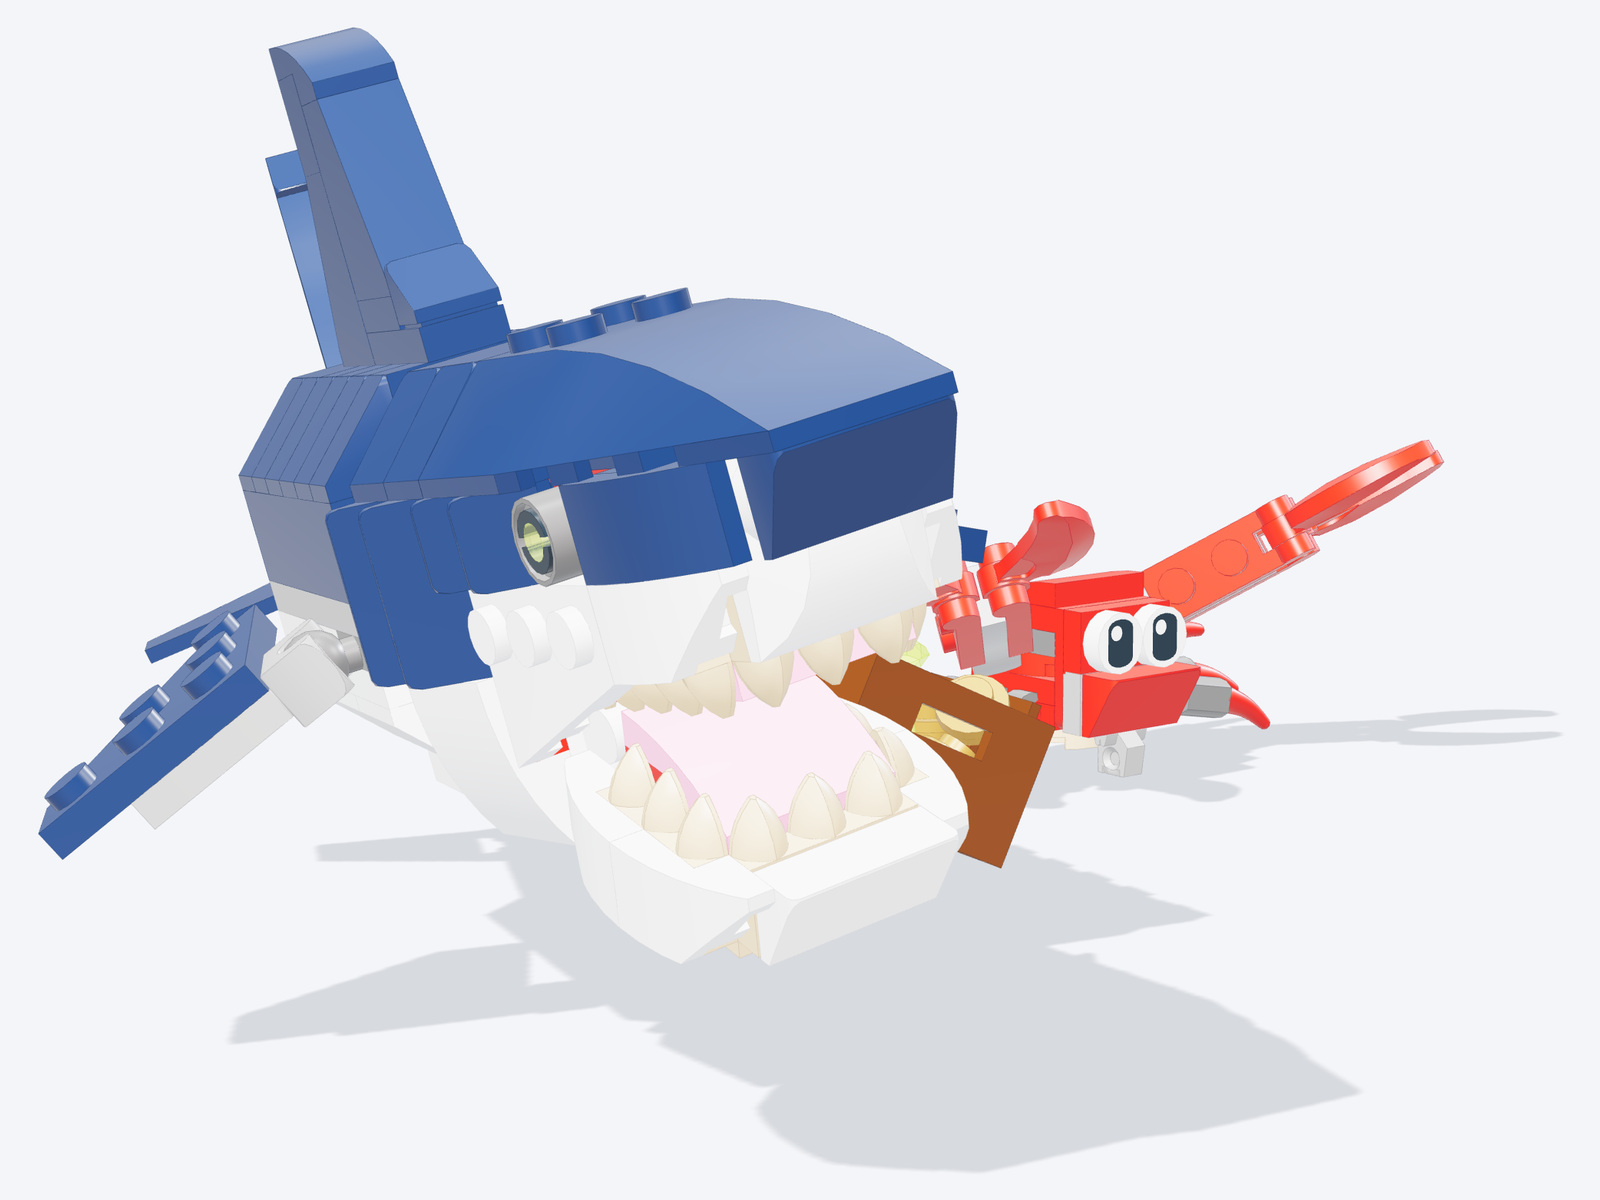
\includegraphics[width=.48\linewidth]{figures/ldraw/print/omr-31088-side.jpg}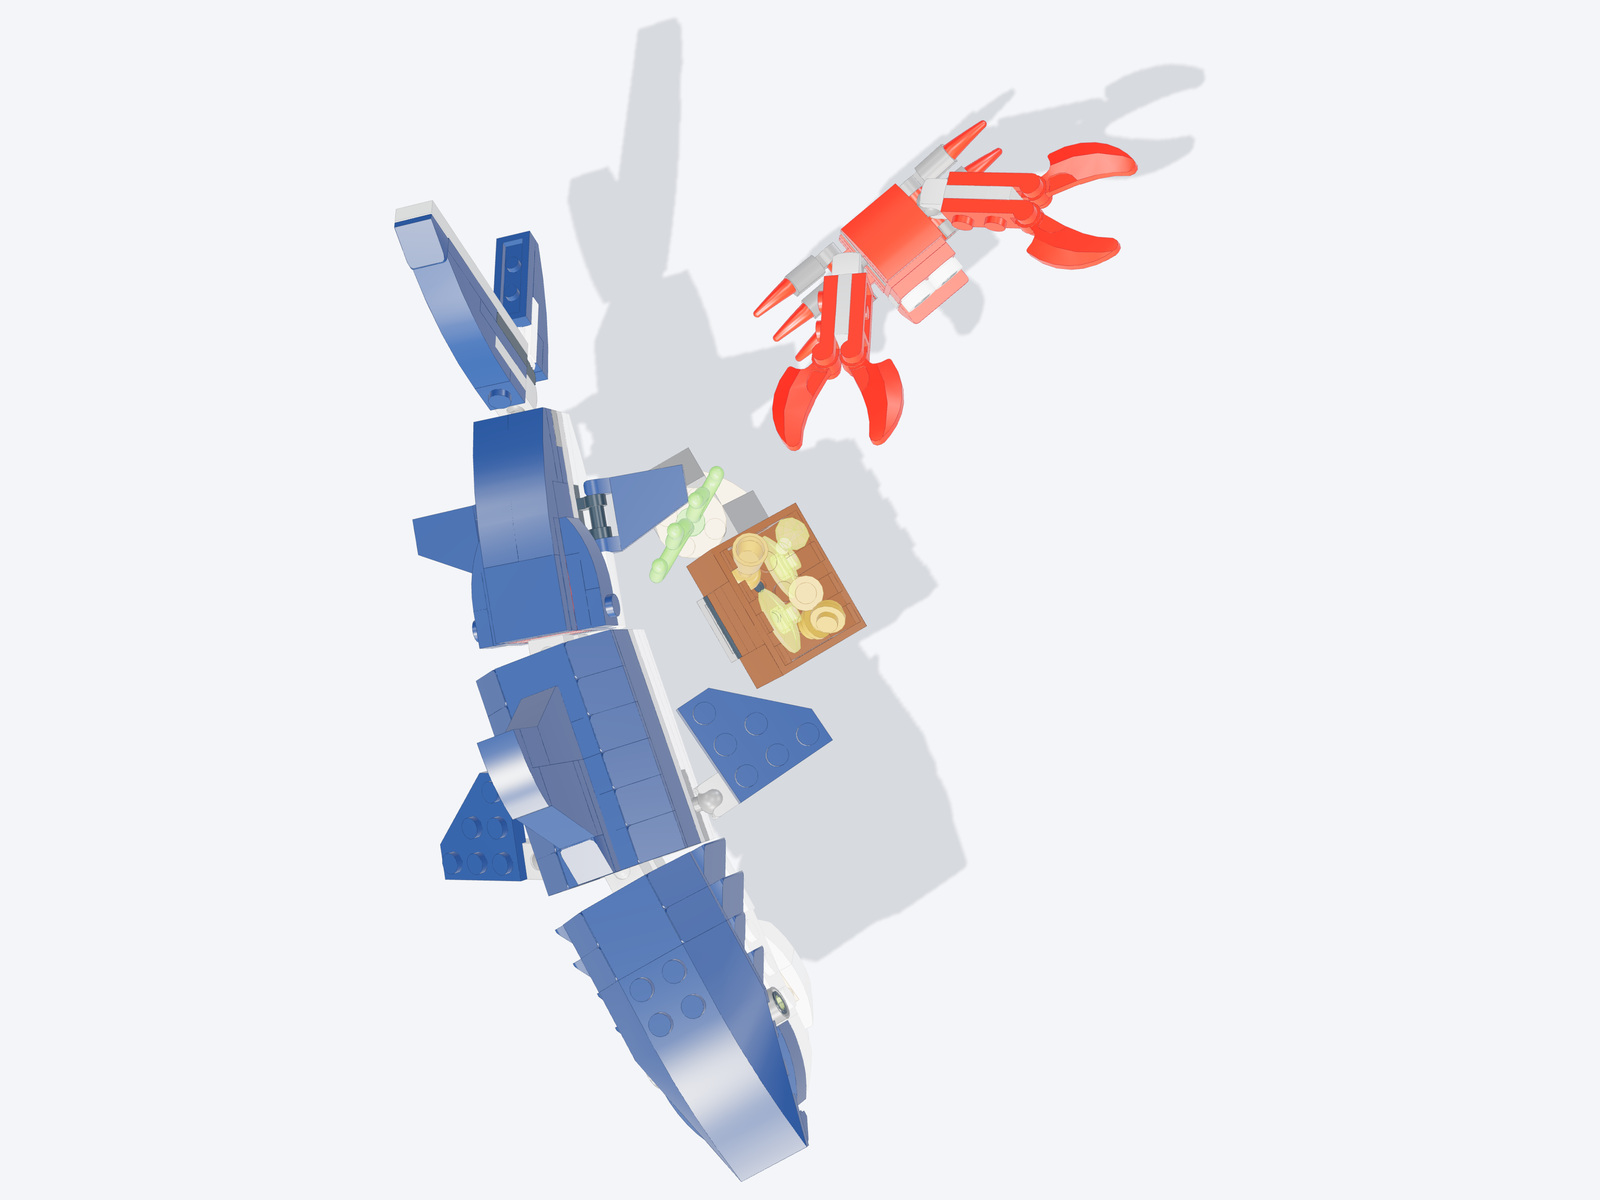
\includegraphics[width=.48\linewidth]{figures/ldraw/print/omr-31088-top.jpg}\end{center}
\paragraph{Attribution.}Marc Belanger [MonsieurPoulet]. CC BY 2.0.\par\noindent\url{https://library.ldraw.org/library/omr/31088-1.mpd}
\paragraph{Source lock.}\small\texttt{c5cc0f95664d50244295783163d1ba3c}\\\texttt{73484f4b9bbfca89ada8bb1de0dbfff5}\normalsize
\paragraph{Evidence coverage.}Connector definitions cover 98.26\% of instances. The audit reports 19 recognized-graph components and 4 intersection candidates without a recognized mating pair. 4 instances have no connector definition. These counts do not certify physical defects or gravitational stability.
\paragraph{Instructions.}98 expanded author steps.
\clearpage\subsection{Numbered visual input and complete question index}
Only relevant numbers are shown. The website can isolate any instance; public visual tasks provide their own numbered images. The following entries give every English prompt, all choice options, compact public evidence and the reference output. Raw repeated connector records and full action fact sets remain in the versioned JSON.
\begin{center}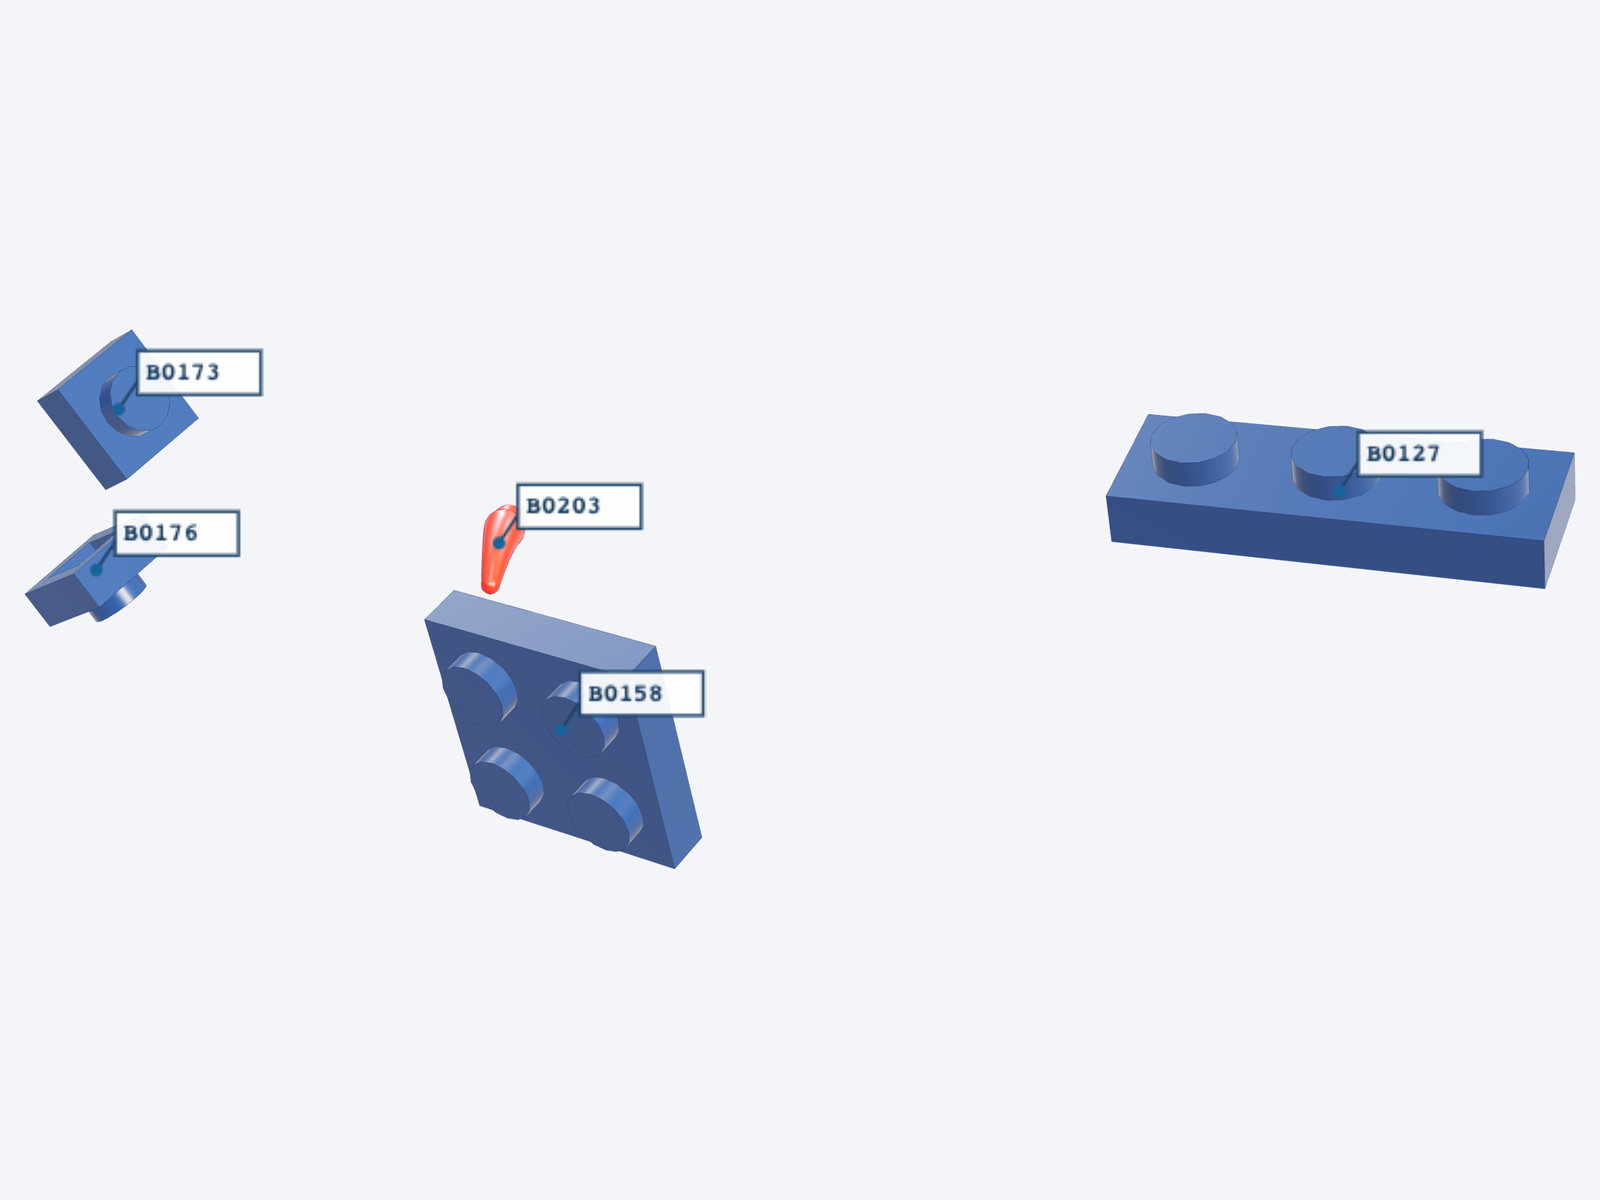
\includegraphics[width=.55\linewidth]{figures/ldraw/print/omr-31088-numbered.jpg}\end{center}
\begin{enumerate}
\item \textbf{color-1}. Identify the original color of B0176; numbered isolation is allowed.\par {\small \textit{Input:} Numbered visual input; source attributes are withheld from the model. \par\textit{Options:} A: Dark Blue; B: Bright Pink; C: Red; D: Pearl Gold. \par\textit{Reference output:} A.}
\item \textbf{shape-match-1}. Ignoring color and pose, which numbered instance has the same LDraw part type as B0176?\par {\small \textit{Input:} Numbered visual input; source attributes are withheld from the model. \par\textit{Options:} A: B0158; B: B0203; C: B0173; D: B0127. \par\textit{Reference output:} C.}
\item \textbf{distance-1}. Using the supplied geometry bounding-box centers, which candidate is nearest to B0176?\par {\small \textit{Input:} Centers (mm): B0176 = (-33.556, 26.7832, -46.9752); B0134 = (-22.2252, 26.8516, -9.6216); B0218 = (55.2016, 12, -67.3224); B0219 = (60.4518, 12, -67.413). \par\textit{Options:} A: B0219; B: B0218; C: B0134. \par\textit{Reference output:} C.}
\item \textbf{color-2}. Identify the original color of B0038; numbered isolation is allowed.\par {\small \textit{Input:} Numbered visual input; source attributes are withheld from the model. \par\textit{Options:} A: Pearl Gold; B: White; C: Trans Neon Green; D: Reddish Brown. \par\textit{Reference output:} B.}
\item \textbf{distance-2}. Using the supplied geometry bounding-box centers, which candidate is nearest to B0038?\par {\small \textit{Input:} Centers (mm): B0038 = (18.2528, 49.856, 114.62); B0189 = (22.964412, 16.89552, 11.27296); B0170 = (-48.90888, 71.1572, -64.25804); B0063 = (24.036997, 55.442263, 103.184794). \par\textit{Options:} A: B0063; B: B0170; C: B0189. \par\textit{Reference output:} A.}
\item \textbf{interface-1}. Classify the supplied connector record for B0210 and B0211. This does not certify load capacity.\par {\small \textit{Input:} Record: family = axle; connector indices = 1, 0. \par\textit{Options:} A: fixed; B: hinge; C: axle; D: ball. \par\textit{Reference output:} C.}
\item \textbf{interface-2}. Classify the supplied connector record for B0089 and B0124. This does not certify load capacity.\par {\small \textit{Input:} Record: family = ball; connector indices = 3, 3. \par\textit{Options:} A: ball; B: fixed; C: hinge; D: axle. \par\textit{Reference output:} A.}
\item \textbf{interface-3}. Classify the supplied connector record for B0184 and B0180. This does not certify load capacity.\par {\small \textit{Input:} Record: family = hinge; connector indices = 6, 2. \par\textit{Options:} A: axle; B: hinge; C: fixed; D: ball. \par\textit{Reference output:} B.}
\item \textbf{interface-4}. Classify the supplied connector record for B0043 and B0044. This does not certify load capacity.\par {\small \textit{Input:} Record: family = stud; connector indices = 5, 2. \par\textit{Options:} A: fixed; B: stud; C: hinge; D: axle; E: ball. \par\textit{Reference output:} B.}
\item \textbf{neighbors-1}. Select every candidate directly adjacent to B0045 in the supplied connector graph.\par {\small \textit{Input:} Unique undirected pairs: B0043 / B0045; B0045 / B0057; B0045 / B0061; B0057 / B0061. \par\textit{Options:} A: B0057; B: B0039; C: B0061; D: B0081; E: B0043. \par\textit{Reference output:} A, C, E.}
\item \textbf{graph-removal-1}. Delete B0045 and its incident edges from this local graph. How many connected components remain? Do not infer physical extractability.\par {\small \textit{Input:} Nodes: B0045, B0043, B0057, B0061, B0081, B0039. Unique undirected pairs: B0043 / B0045; B0045 / B0057; B0045 / B0061; B0057 / B0061. \par\textit{Options:} A: 4; B: 5; C: 3; D: 6. \par\textit{Reference output:} A.}
\item \textbf{neighbors-2}. Select every candidate directly adjacent to B0120 in the supplied connector graph.\par {\small \textit{Input:} Unique undirected pairs: B0116 / B0120; B0117 / B0120; B0120 / B0127. \par\textit{Options:} A: B0072; B: B0117; C: B0094; D: B0116; E: B0127. \par\textit{Reference output:} B, D, E.}
\item \textbf{graph-removal-2}. Delete B0120 and its incident edges from this local graph. How many connected components remain? Do not infer physical extractability.\par {\small \textit{Input:} Nodes: B0120, B0116, B0127, B0117, B0094, B0072. Unique undirected pairs: B0116 / B0120; B0117 / B0120; B0120 / B0127. \par\textit{Options:} A: 5; B: 7; C: 6; D: 4. \par\textit{Reference output:} A.}
\item \textbf{coverage-1}. Which numbered instance lacks a connector definition in the coverage record, so this audit cannot establish that it is floating?\par {\small \textit{Input:} Definition coverage: B0092 = unsupported; B0176 = supported; B0038 = supported; B0181 = supported. \par\textit{Options:} A: B0176; B: B0092; C: B0181; D: B0038. \par\textit{Reference output:} B.}
\item \textbf{evidence-limit-1}. Only source geometry, connector matching and mesh intersection audits are available. Without mass, friction, material or dynamic tests, is gravitational stability established?\par {\small \textit{Input:} Available evidence: Original CAD; Connector inference; Inset-mesh intersection candidates. \par\textit{Options:} A: Not established by this evidence; B: Established. \par\textit{Reference output:} A.}
\item \textbf{source-step-1}. At which expanded author step does B0184 first appear in the supplied source-step table? Source order is not a collision-free assembly proof.\par {\small \textit{Input:} Expanded author records: step 1: B0001; step 85: B0184. \par\textit{Options:} A: 87; B: 84; C: 85; D: 86. \par\textit{Reference output:} C.}
\item \textbf{source-step-2}. At which expanded author step does B0083 first appear in the supplied source-step table? Source order is not a collision-free assembly proof.\par {\small \textit{Input:} Expanded author records: step 1: B0001; step 44: B0083. \par\textit{Options:} A: 43; B: 46; C: 44; D: 45. \par\textit{Reference output:} C.}
\item \textbf{source-sequence-1}. Reveal the supplied source-step window in author order. Actions change visibility only, without simulating insertion trajectories.\par {\small \textit{Input:} Source window: step-1: B0001, B0002; step-2: B0003; step-3: B0004; step-4: B0005; step-5: B0006, B0007; step-6: B0008, B0009. Action budget: 6. \par\textit{Reference output:} step-1, step-2, step-3, step-4, step-5, step-6.}
\item \textbf{restore-instance-1}. The display copy hides B0176. Restore only that numbered instance, preserving all other instances and source poses.\par {\small \textit{Input:} Target: B0176. Action budget: 1. All other instances initially remain visible. \par\textit{Reference output:} restore-B0176.}
\item \textbf{restore-instance-2}. The display copy hides B0038. Restore only that numbered instance, preserving all other instances and source poses.\par {\small \textit{Input:} Target: B0038. Action budget: 1. All other instances initially remain visible. \par\textit{Reference output:} restore-B0038.}
\end{enumerate}
\clearpage
\section{42004: Mini Backhoe Loader}
246 source instances; 20 tasks; D2 scale band.

\par\noindent Perspective, front, side and top views follow in reading order. Original source transforms are preserved.
\begin{center}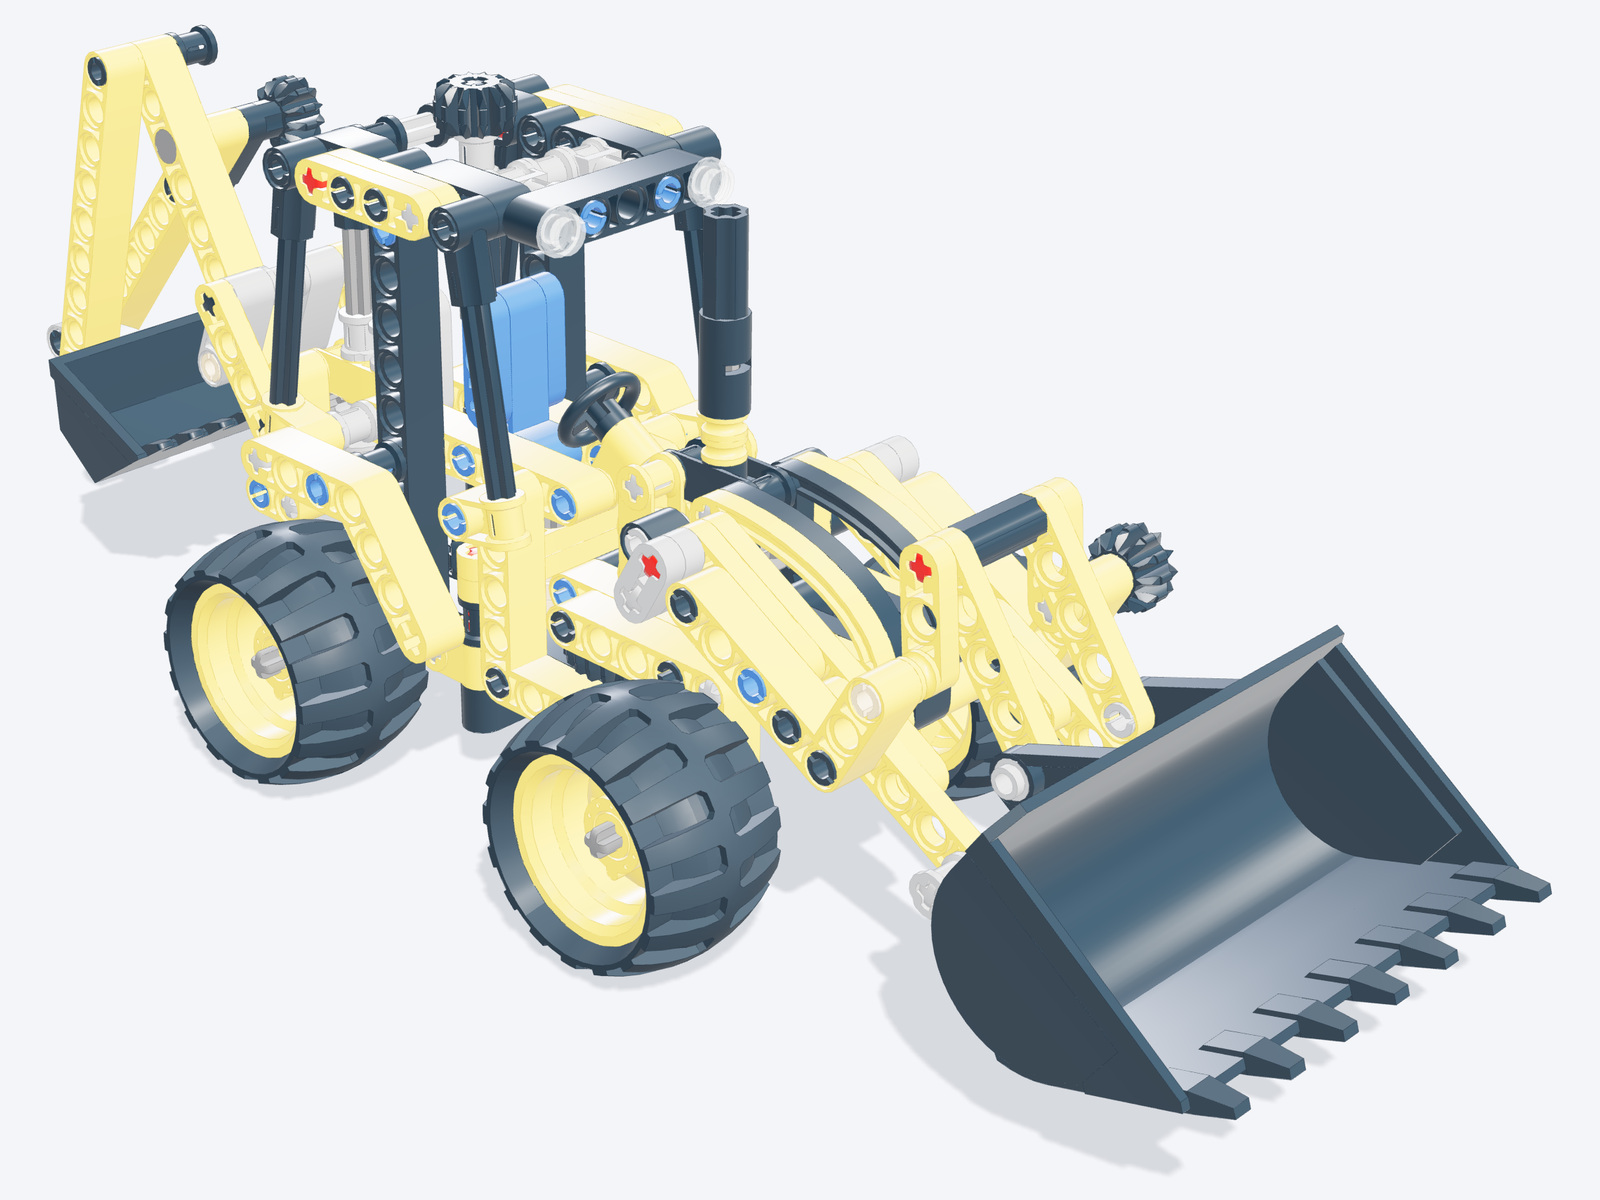
\includegraphics[width=.48\linewidth]{figures/ldraw/print/omr-42004-iso.jpg}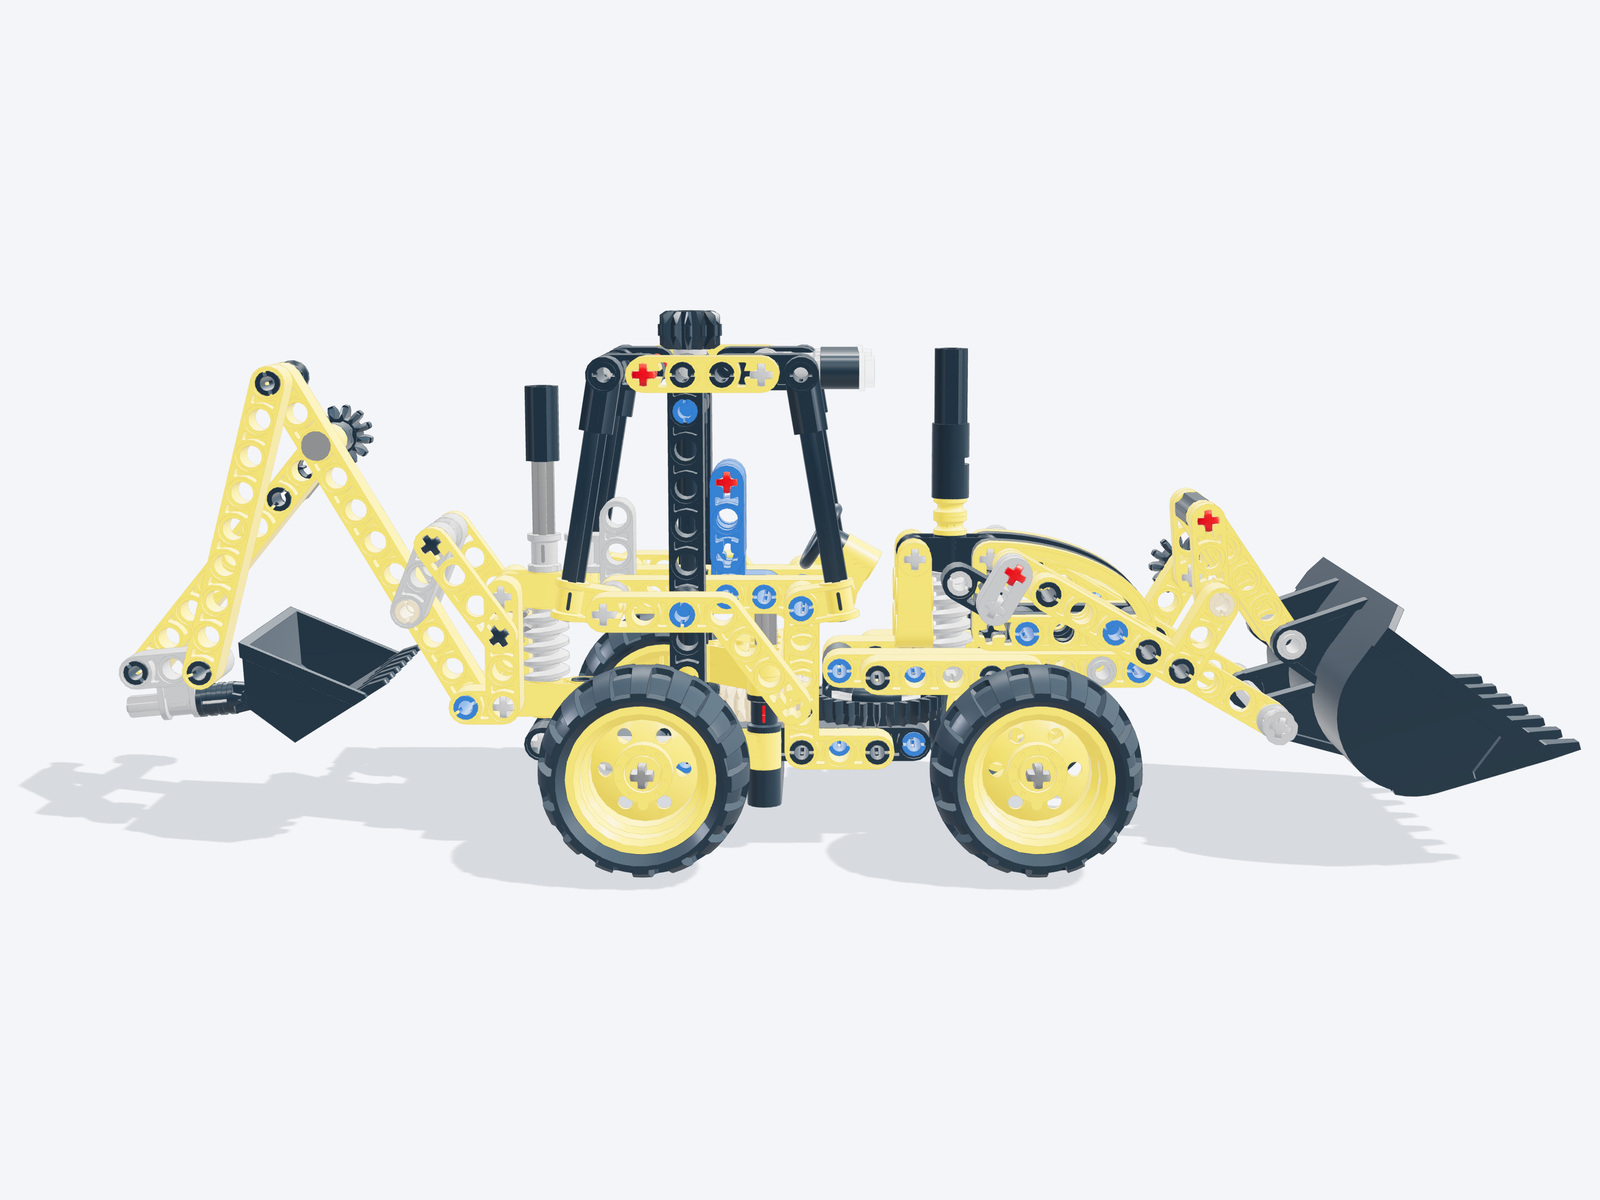
\includegraphics[width=.48\linewidth]{figures/ldraw/print/omr-42004-front.jpg}\\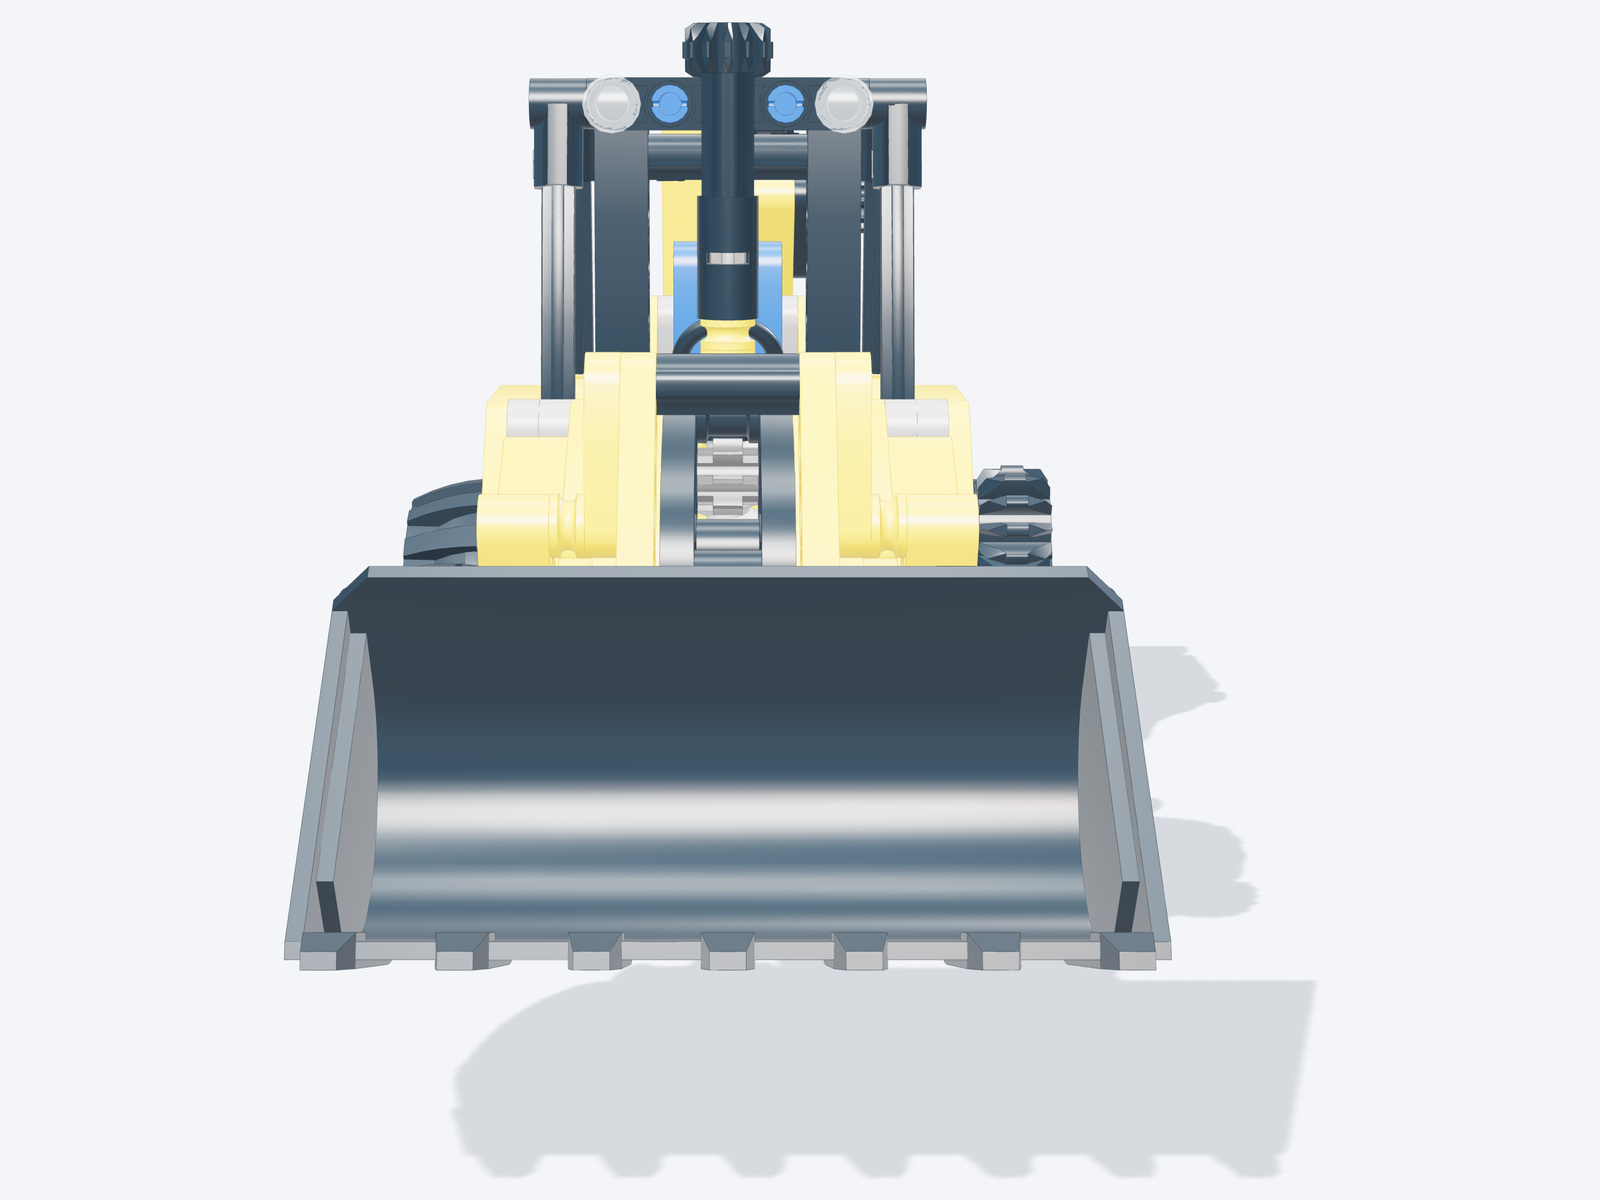
\includegraphics[width=.48\linewidth]{figures/ldraw/print/omr-42004-side.jpg}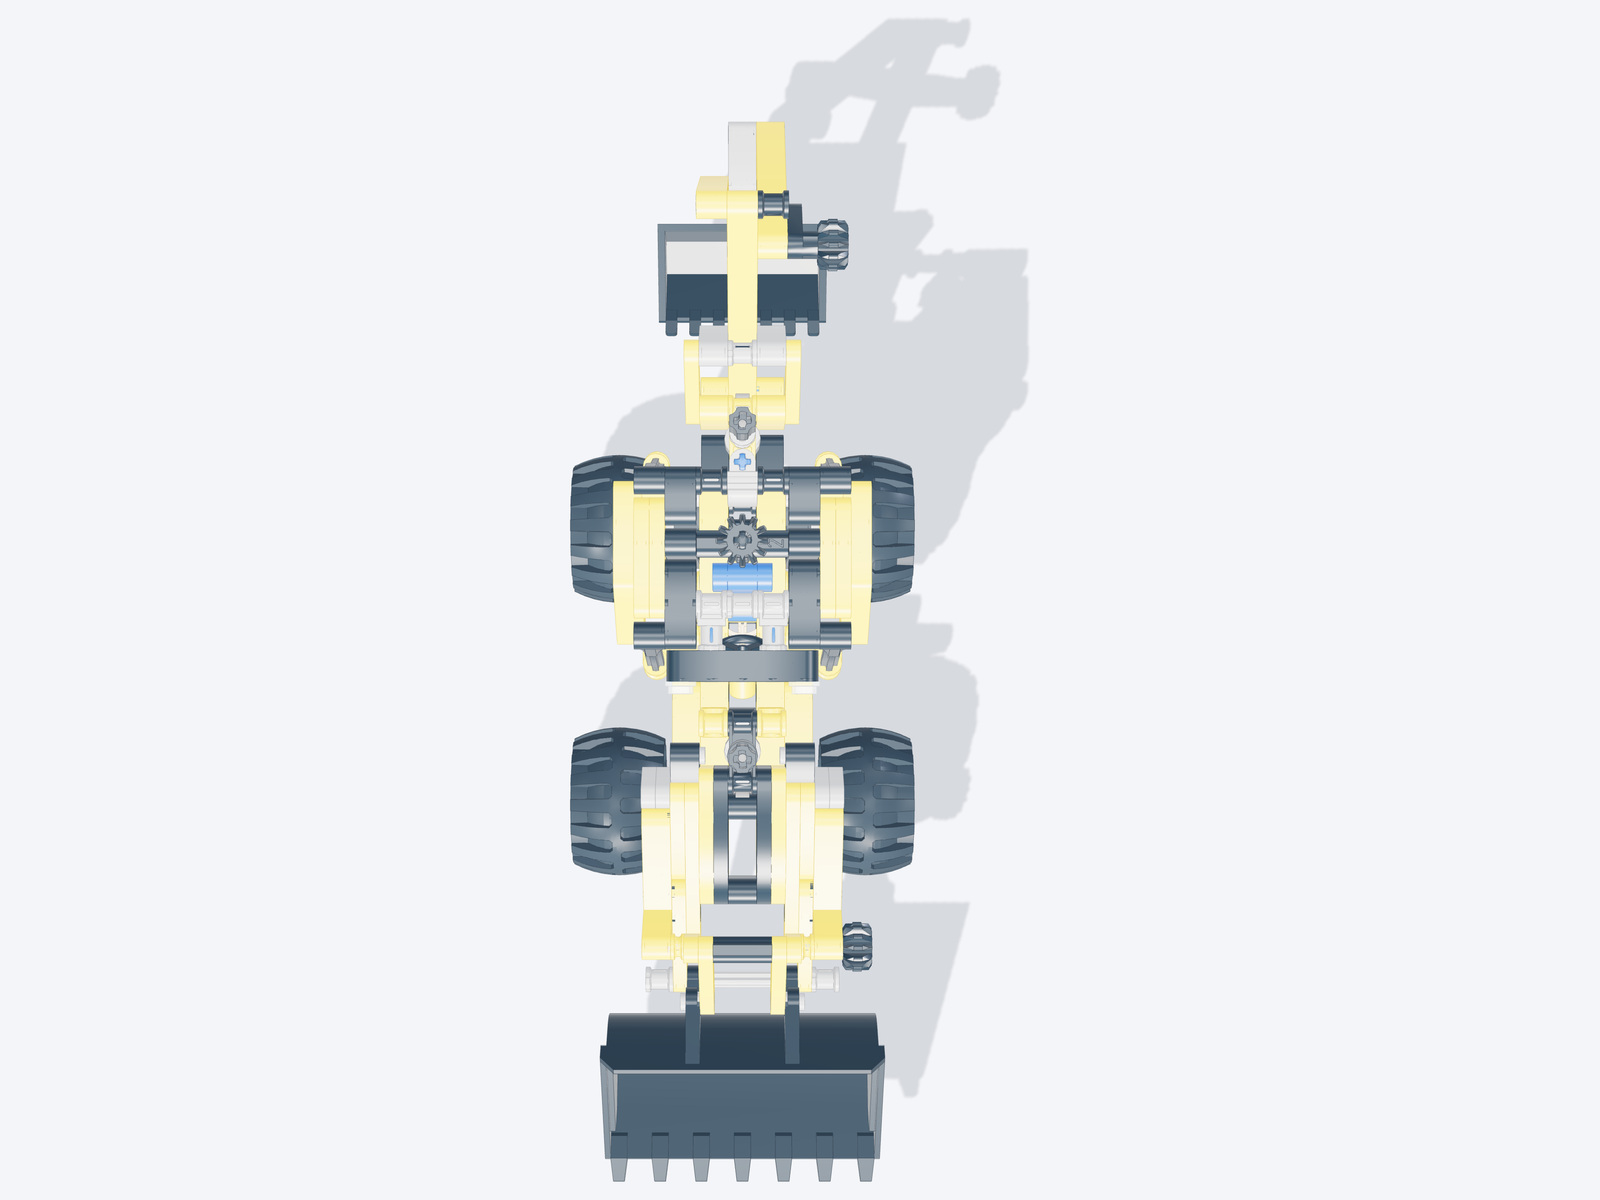
\includegraphics[width=.48\linewidth]{figures/ldraw/print/omr-42004-top.jpg}\end{center}
\paragraph{Attribution.}Tomas Kralicek [RabbiT\_CZ]. CC BY 2.0.\par\noindent\url{https://library.ldraw.org/library/omr/42004-1.mpd}
\paragraph{Source lock.}\small\texttt{a32b924f302a1c028c1131f78e438ad2}\\\texttt{d78e70a041999690a1e4285e851f7dbf}\normalsize
\paragraph{Evidence coverage.}Connector definitions cover 100.00\% of instances. The audit reports 2 recognized-graph components and 4 intersection candidates without a recognized mating pair. 0 instances have no connector definition. These counts do not certify physical defects or gravitational stability.
\paragraph{Instructions.}86 expanded author steps.
\clearpage\subsection{Numbered visual input and complete question index}
Only relevant numbers are shown. The website can isolate any instance; public visual tasks provide their own numbered images. The following entries give every English prompt, all choice options, compact public evidence and the reference output. Raw repeated connector records and full action fact sets remain in the versioned JSON.
\begin{center}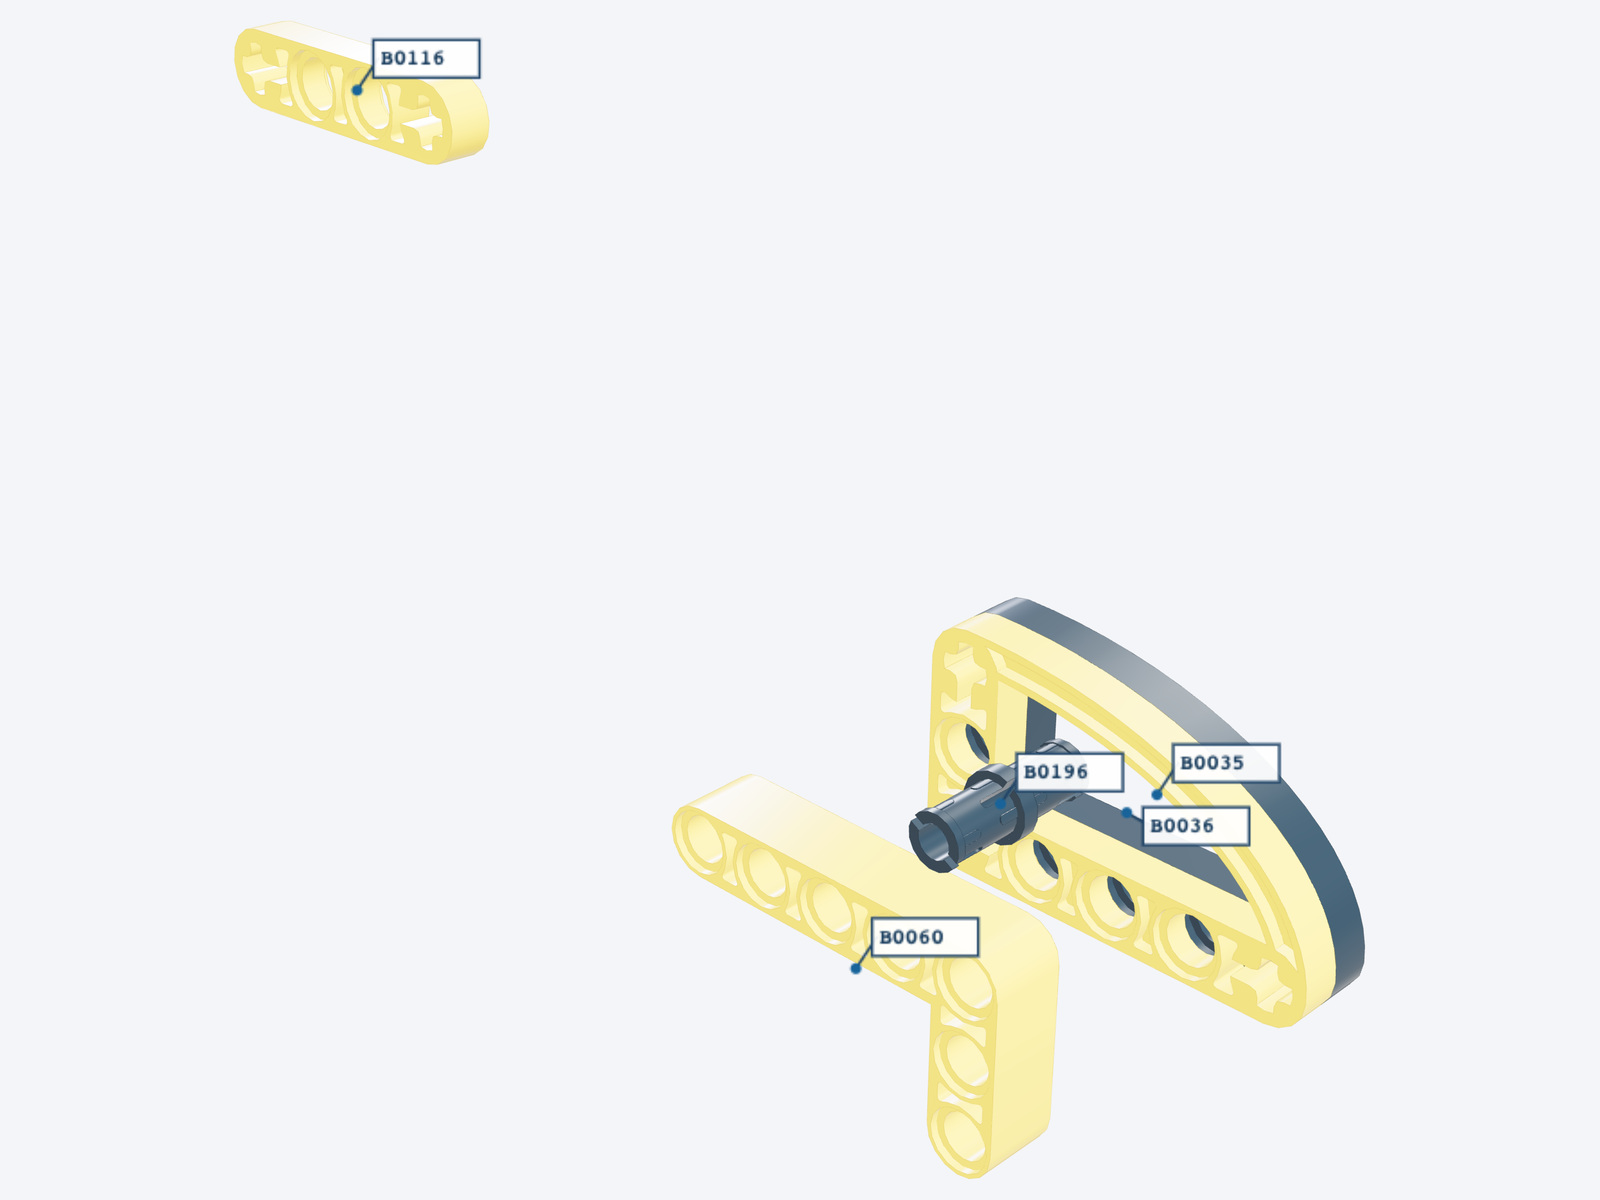
\includegraphics[width=.55\linewidth]{figures/ldraw/print/omr-42004-numbered.jpg}\end{center}
\begin{enumerate}
\item \textbf{color-1}. Identify the original color of B0035; numbered isolation is allowed.\par {\small \textit{Input:} Numbered visual input; source attributes are withheld from the model. \par\textit{Options:} A: Rubber Black; B: Black; C: Tan; D: Blue. \par\textit{Reference output:} B.}
\item \textbf{shape-match-1}. Ignoring color and pose, which numbered instance has the same LDraw part type as B0035?\par {\small \textit{Input:} Numbered visual input; source attributes are withheld from the model. \par\textit{Options:} A: B0060; B: B0036; C: B0196; D: B0116. \par\textit{Reference output:} B.}
\item \textbf{distance-1}. Using the supplied geometry bounding-box centers, which candidate is nearest to B0035?\par {\small \textit{Input:} Centers (mm): B0035 = (2, 32, 72); B0171 = (20, 57.456642, -92.888958); B0233 = (20.8, 22.3832, 119.5668); B0116 = (-18, 80, -4). \par\textit{Options:} A: B0171; B: B0233; C: B0116. \par\textit{Reference output:} B.}
\item \textbf{color-2}. Identify the original color of B0191; numbered isolation is allowed.\par {\small \textit{Input:} Numbered visual input; source attributes are withheld from the model. \par\textit{Options:} A: Black; B: Light Bluish Grey; C: Rubber Black; D: Yellow. \par\textit{Reference output:} A.}
\item \textbf{shape-match-2}. Ignoring color and pose, which numbered instance has the same LDraw part type as B0191?\par {\small \textit{Input:} Numbered visual input; source attributes are withheld from the model. \par\textit{Options:} A: B0047; B: B0141; C: B0235; D: B0039. \par\textit{Reference output:} B.}
\item \textbf{distance-2}. Using the supplied geometry bounding-box centers, which candidate is nearest to B0191?\par {\small \textit{Input:} Centers (mm): B0191 = (-16, 52.39, -28.712); B0003 = (8, 0, 24); B0172 = (32, 63.4256, -88); B0082 = (24, 16, 24). \par\textit{Options:} A: B0003; B: B0082; C: B0172. \par\textit{Reference output:} B.}
\item \textbf{interface-1}. Classify the supplied connector record for B0047 and B0041. This does not certify load capacity.\par {\small \textit{Input:} Record: family = axle; connector indices = 0, 0. \par\textit{Options:} A: ball; B: axle; C: fixed; D: hinge. \par\textit{Reference output:} B.}
\item \textbf{interface-2}. Classify the supplied connector record for B0239 and B0240. This does not certify load capacity.\par {\small \textit{Input:} Record: family = fixed; connector indices = 2, 1. \par\textit{Options:} A: ball; B: hinge; C: fixed; D: axle. \par\textit{Reference output:} C.}
\item \textbf{interface-3}. Classify the supplied connector record for B0179 and B0178. This does not certify load capacity.\par {\small \textit{Input:} Record: family = hinge; connector indices = 1, 0. \par\textit{Options:} A: hinge; B: ball; C: fixed; D: axle. \par\textit{Reference output:} A.}
\item \textbf{interface-4}. Classify the supplied connector record for B0146 and B0145. This does not certify load capacity.\par {\small \textit{Input:} Record: family = stud; connector indices = 1, 5. \par\textit{Options:} A: fixed; B: axle; C: stud; D: ball; E: hinge. \par\textit{Reference output:} C.}
\item \textbf{neighbors-1}. Select every candidate directly adjacent to B0192 in the supplied connector graph.\par {\small \textit{Input:} Unique undirected pairs: B0129 / B0192; B0191 / B0192. \par\textit{Options:} A: B0099; B: B0129; C: B0191; D: B0015. \par\textit{Reference output:} B, C.}
\item \textbf{graph-removal-1}. Delete B0192 and its incident edges from this local graph. How many connected components remain? Do not infer physical extractability.\par {\small \textit{Input:} Nodes: B0192, B0129, B0191, B0099, B0015. Unique undirected pairs: B0129 / B0192; B0191 / B0192. \par\textit{Options:} A: 5; B: 4; C: 6; D: 3. \par\textit{Reference output:} B.}
\item \textbf{neighbors-2}. Select every candidate directly adjacent to B0180 in the supplied connector graph.\par {\small \textit{Input:} Unique undirected pairs: B0173 / B0180; B0176 / B0180. \par\textit{Options:} A: B0176; B: B0173; C: B0210; D: B0011. \par\textit{Reference output:} A, B.}
\item \textbf{graph-removal-2}. Delete B0180 and its incident edges from this local graph. How many connected components remain? Do not infer physical extractability.\par {\small \textit{Input:} Nodes: B0180, B0176, B0173, B0011, B0210. Unique undirected pairs: B0173 / B0180; B0176 / B0180. \par\textit{Options:} A: 4; B: 3; C: 5; D: 6. \par\textit{Reference output:} A.}
\item \textbf{evidence-limit-1}. Only source geometry, connector matching and mesh intersection audits are available. Without mass, friction, material or dynamic tests, is gravitational stability established?\par {\small \textit{Input:} Available evidence: Original CAD; Connector inference; Inset-mesh intersection candidates. \par\textit{Options:} A: Not established by this evidence; B: Established. \par\textit{Reference output:} A.}
\item \textbf{source-step-1}. At which expanded author step does B0007 first appear in the supplied source-step table? Source order is not a collision-free assembly proof.\par {\small \textit{Input:} Expanded author records: step 1: B0001; step 4: B0007. \par\textit{Options:} A: 3; B: 4; C: 5; D: 6. \par\textit{Reference output:} B.}
\item \textbf{source-step-2}. At which expanded author step does B0150 first appear in the supplied source-step table? Source order is not a collision-free assembly proof.\par {\small \textit{Input:} Expanded author records: step 1: B0001; step 49: B0150. \par\textit{Options:} A: 49; B: 51; C: 48; D: 50. \par\textit{Reference output:} A.}
\item \textbf{source-sequence-1}. Reveal the supplied source-step window in author order. Actions change visibility only, without simulating insertion trajectories.\par {\small \textit{Input:} Source window: step-1: B0001, B0002, B0003; step-2: B0004; step-3: B0005, B0006; step-4: B0007, B0008, B0009, B0010, B0011, B0012; step-5: B0013; step-6: B0014, B0015. Action budget: 6. \par\textit{Reference output:} step-1, step-2, step-3, step-4, step-5, step-6.}
\item \textbf{restore-instance-1}. The display copy hides B0035. Restore only that numbered instance, preserving all other instances and source poses.\par {\small \textit{Input:} Target: B0035. Action budget: 1. All other instances initially remain visible. \par\textit{Reference output:} restore-B0035.}
\item \textbf{restore-instance-2}. The display copy hides B0191. Restore only that numbered instance, preserving all other instances and source poses.\par {\small \textit{Input:} Target: B0191. Action budget: 1. All other instances initially remain visible. \par\textit{Reference output:} restore-B0191.}
\end{enumerate}
\clearpage
\section{42061: Telehandler}
261 source instances; 20 tasks; D2 scale band.

\par\noindent Perspective, front, side and top views follow in reading order. Original source transforms are preserved.
\begin{center}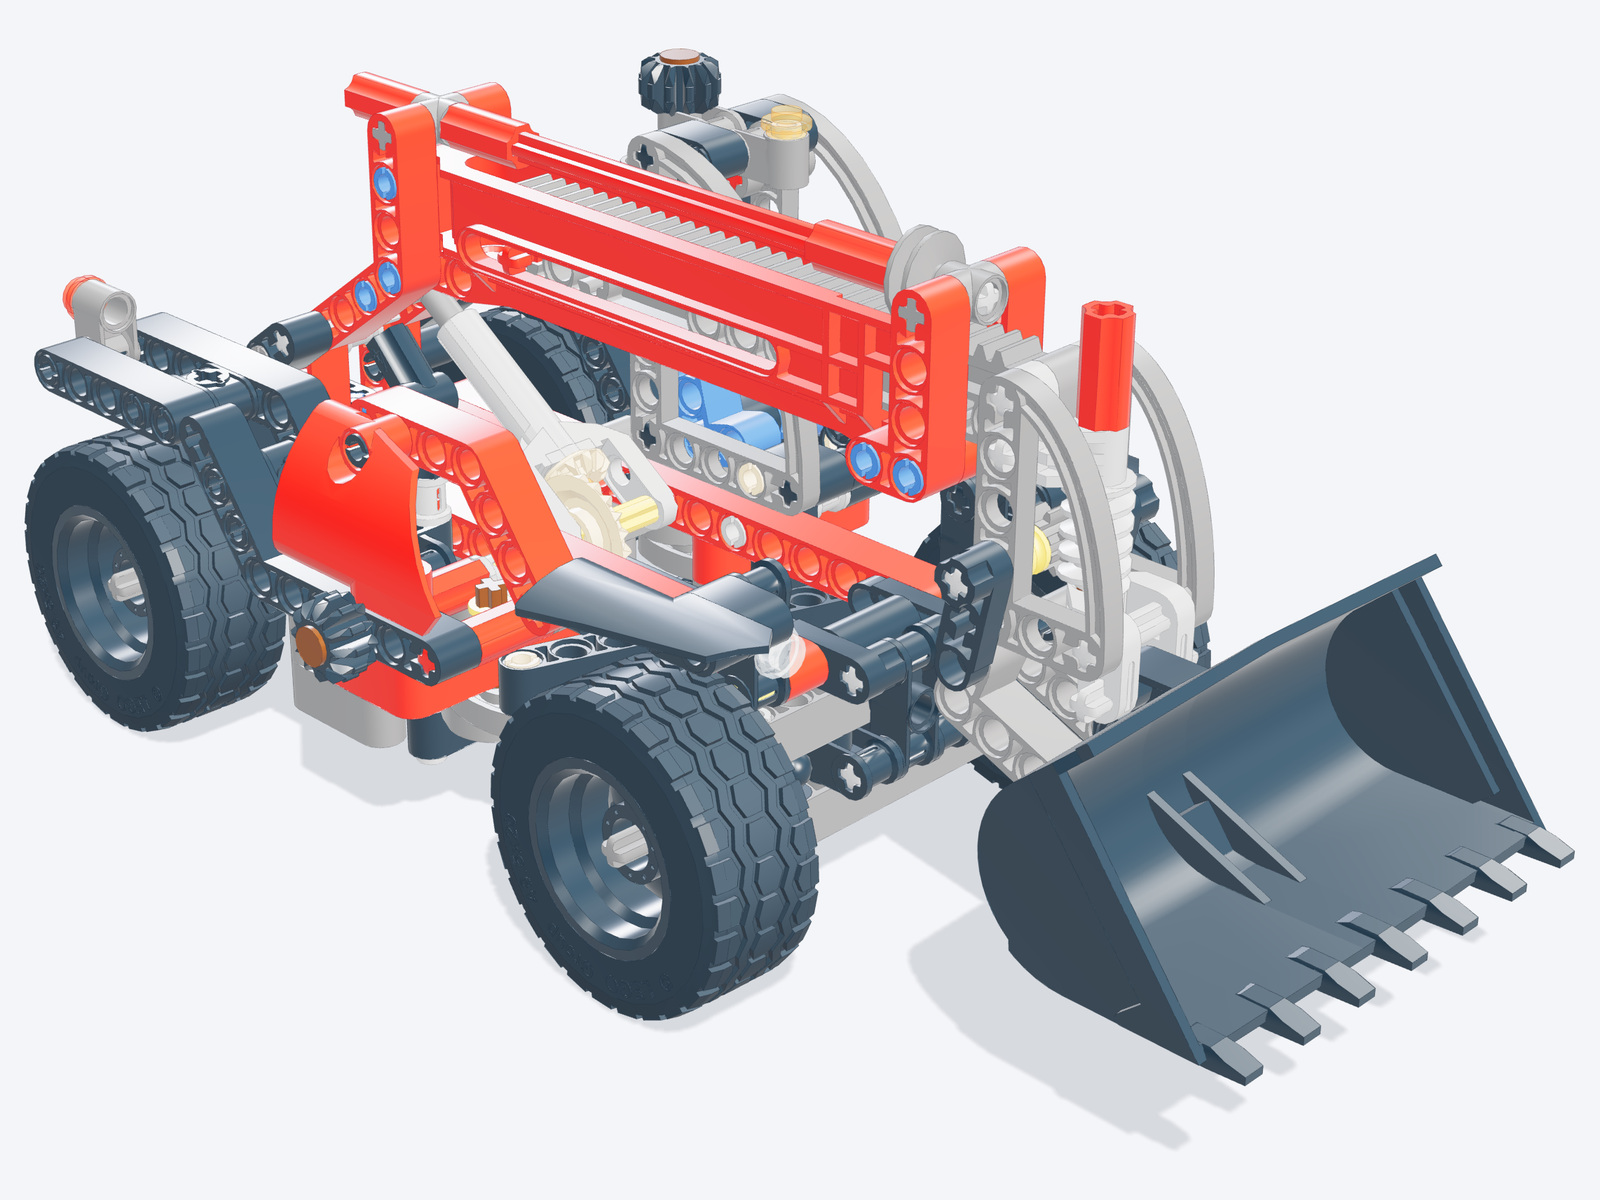
\includegraphics[width=.48\linewidth]{figures/ldraw/print/omr-42061-iso.jpg}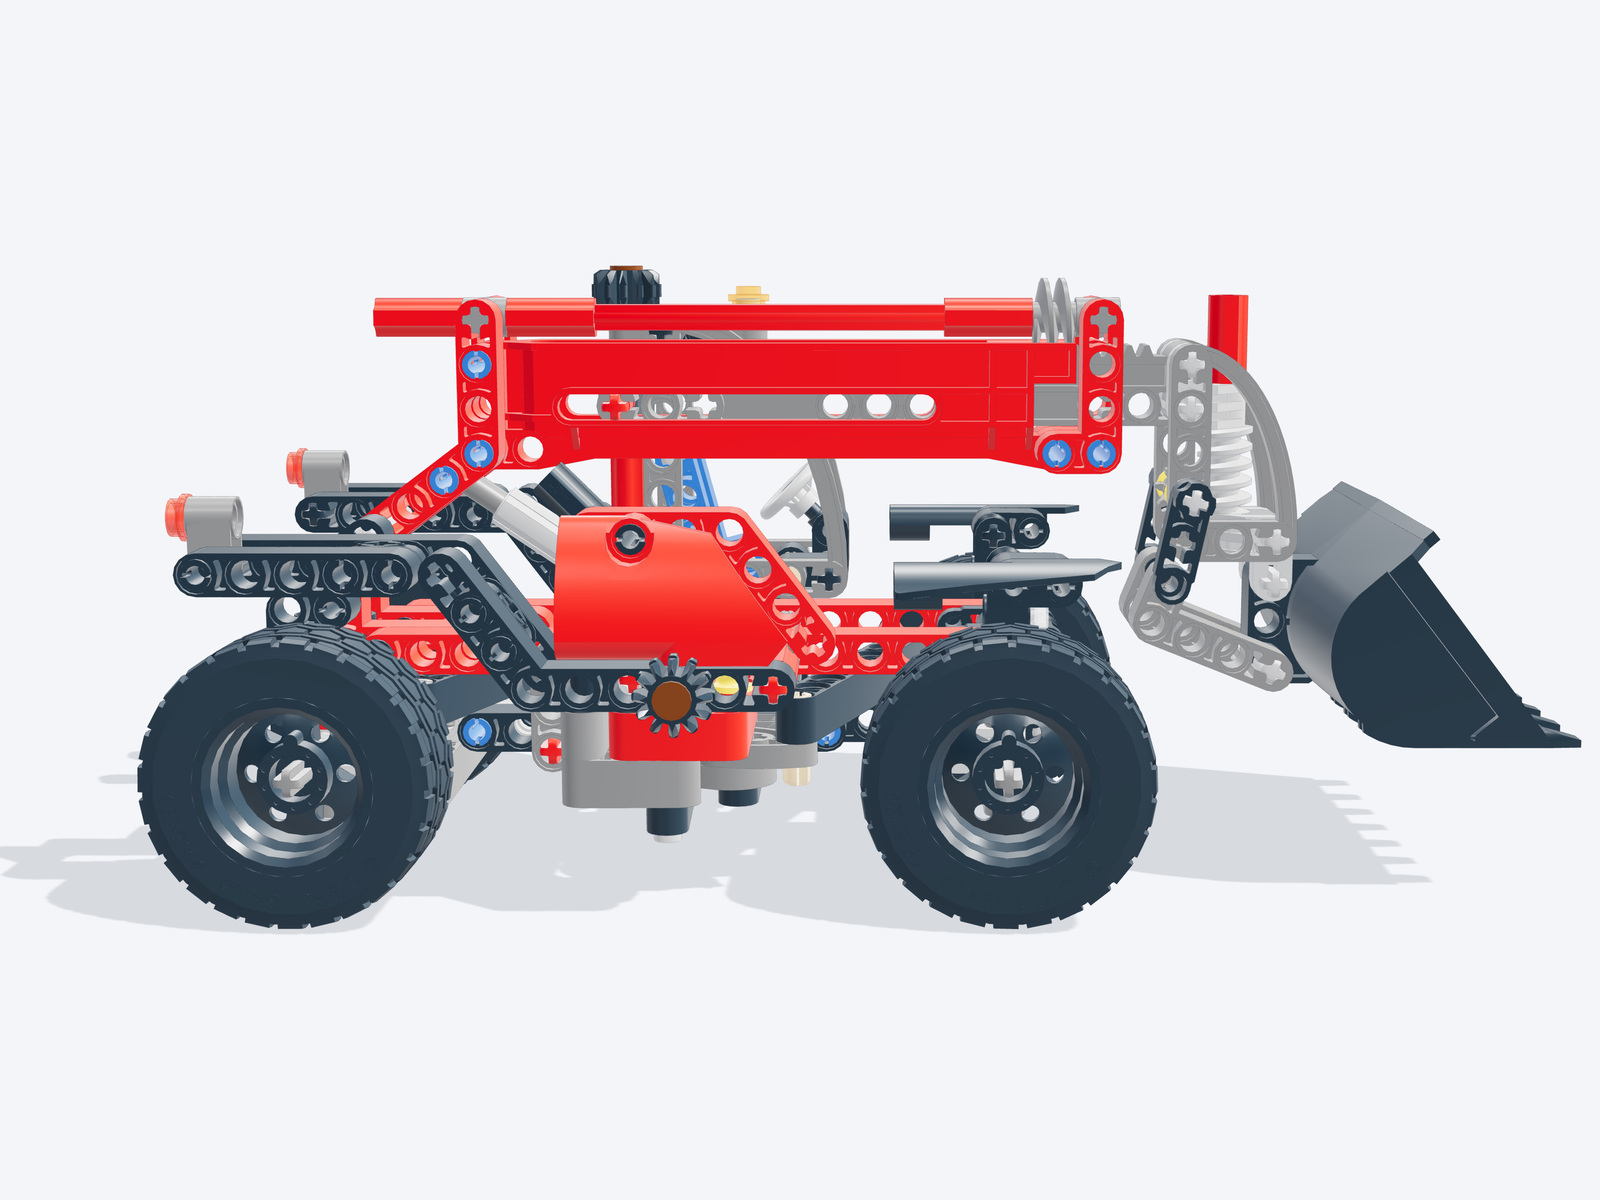
\includegraphics[width=.48\linewidth]{figures/ldraw/print/omr-42061-front.jpg}\\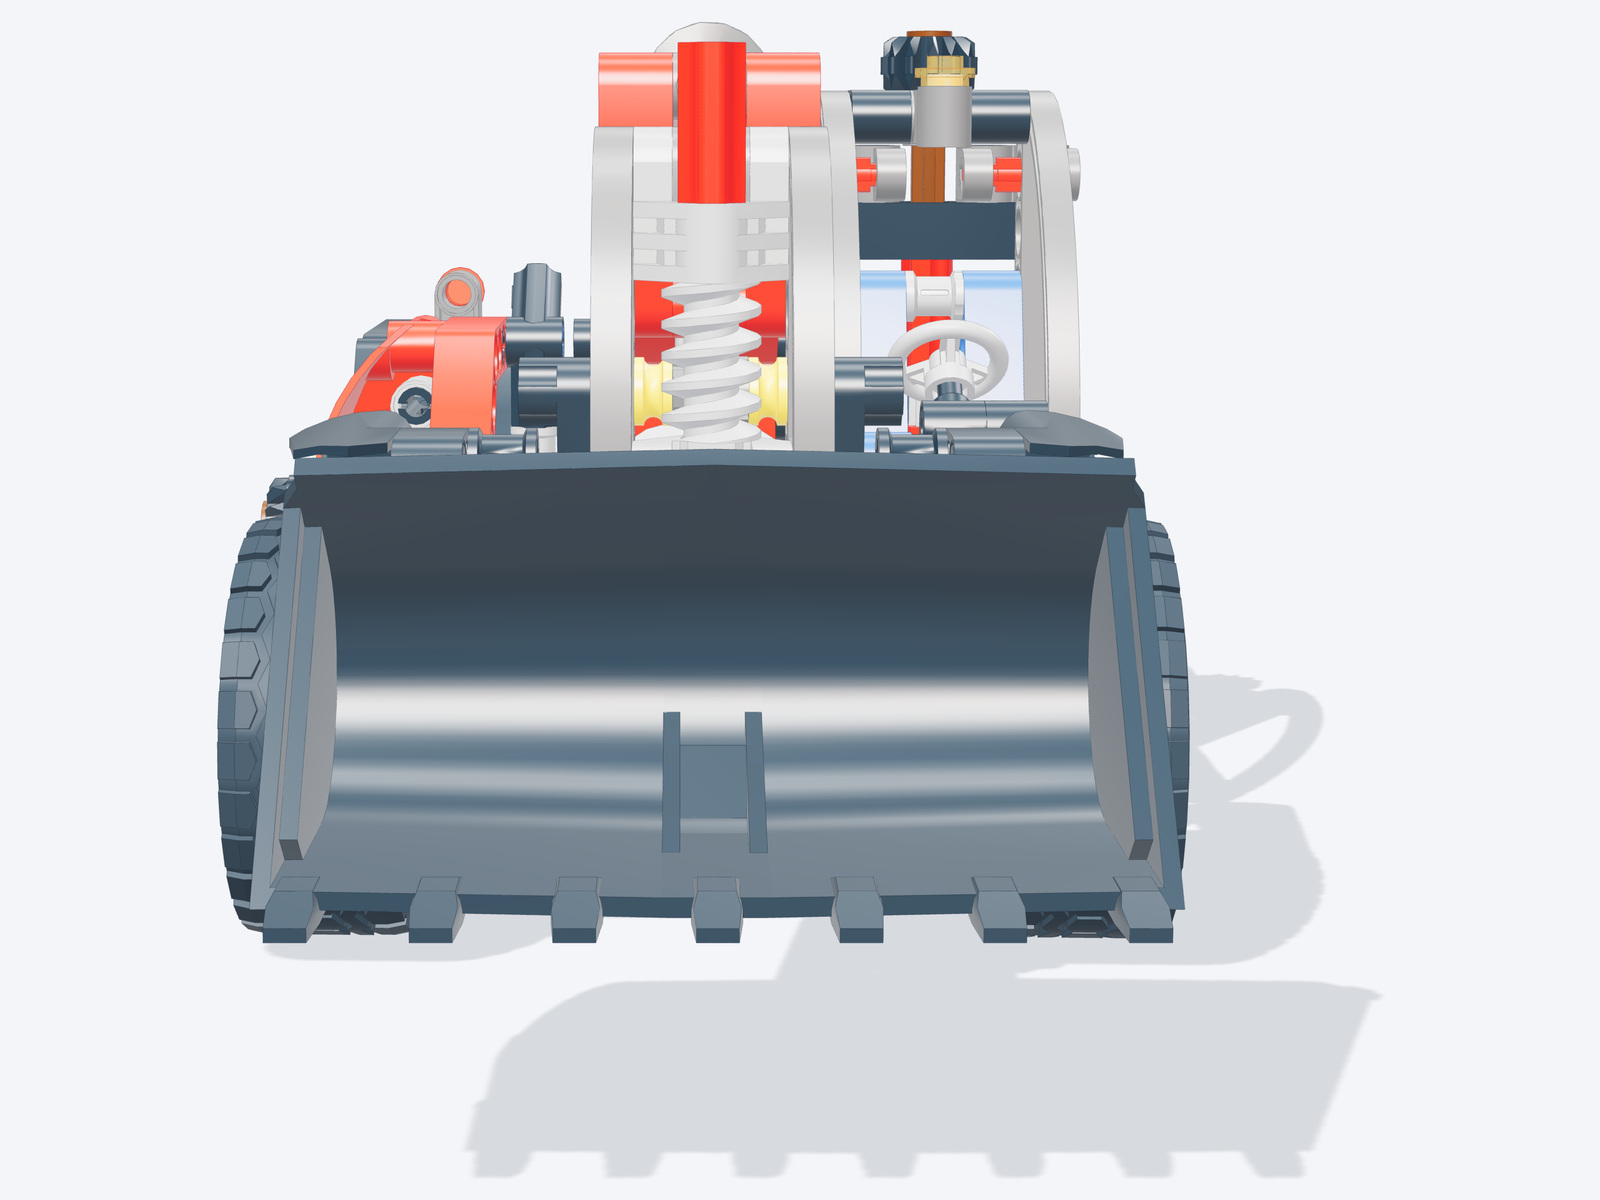
\includegraphics[width=.48\linewidth]{figures/ldraw/print/omr-42061-side.jpg}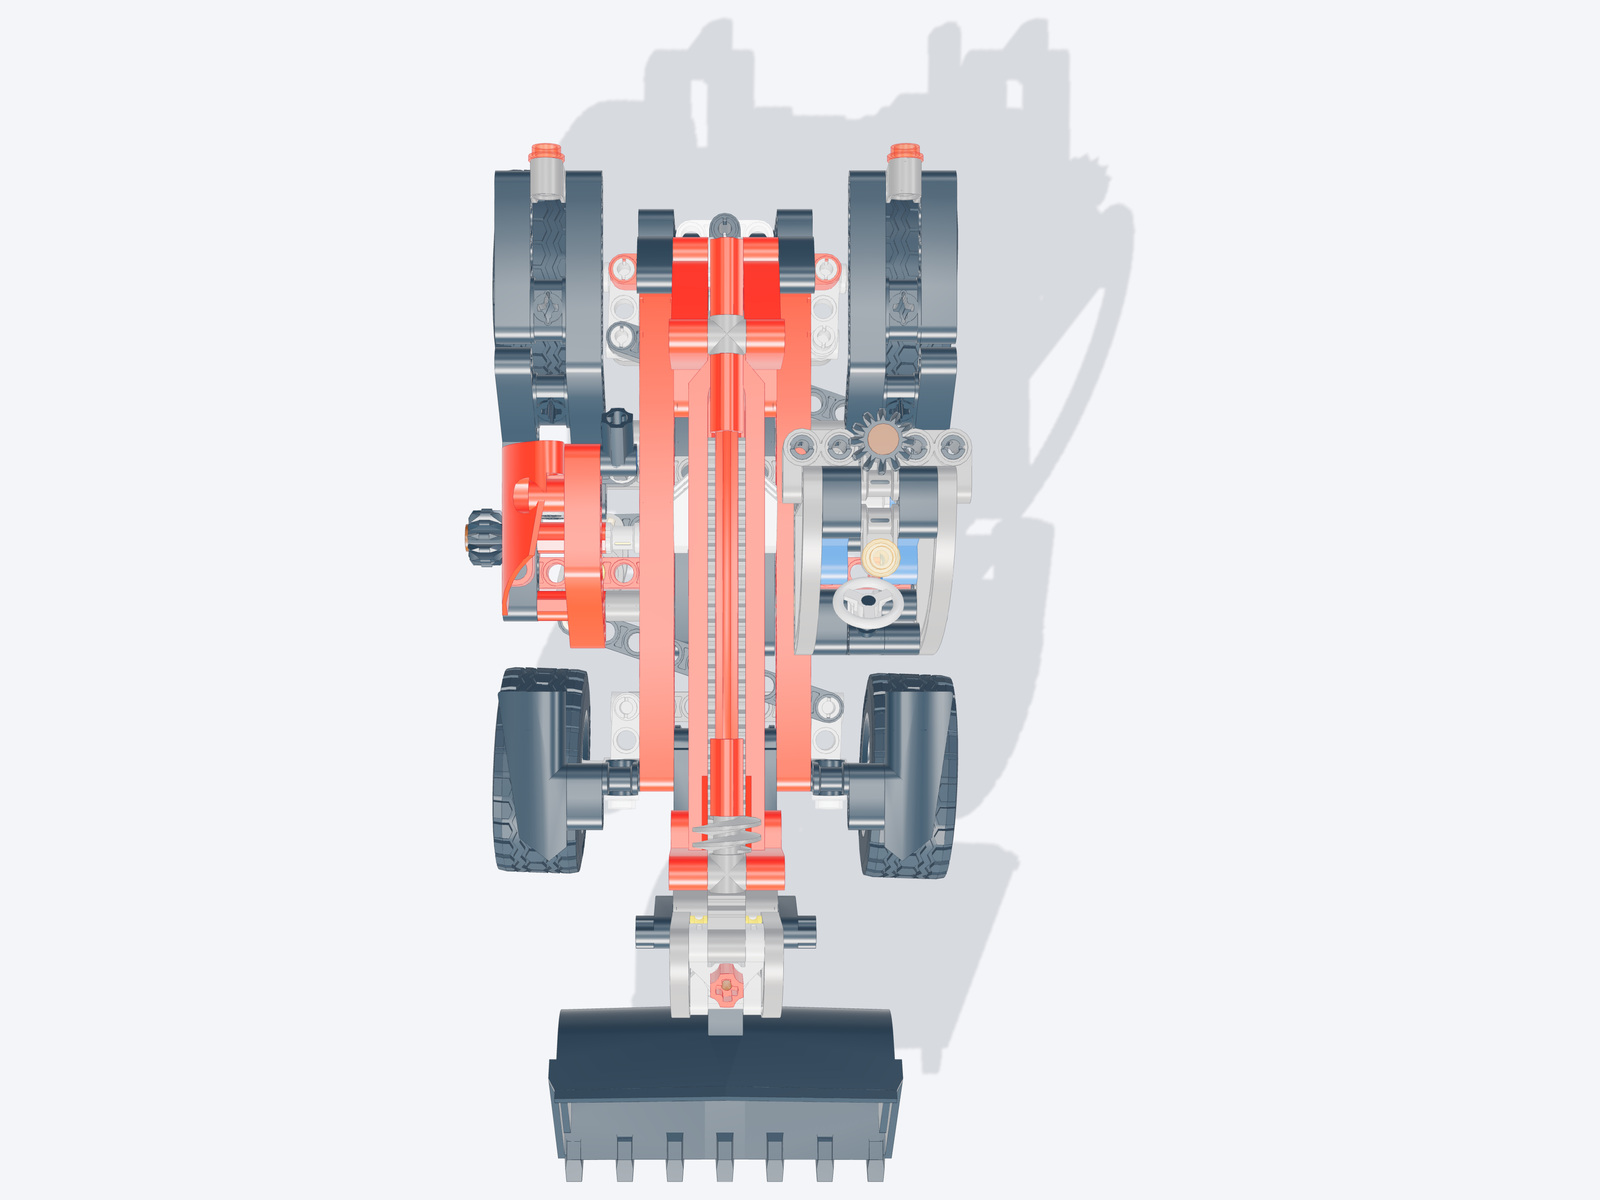
\includegraphics[width=.48\linewidth]{figures/ldraw/print/omr-42061-top.jpg}\end{center}
\paragraph{Attribution.}Philippe Hurbain [Philo]. CC BY 2.0.\par\noindent\url{https://library.ldraw.org/library/omr/42061-1.mpd}
\paragraph{Source lock.}\small\texttt{040a7bd002747abebebca005d7d049c9}\\\texttt{02ffd39d2b102c180458fcfdd94f369c}\normalsize
\paragraph{Evidence coverage.}Connector definitions cover 95.02\% of instances. The audit reports 20 recognized-graph components and 3 intersection candidates without a recognized mating pair. 13 instances have no connector definition. These counts do not certify physical defects or gravitational stability.
\paragraph{Instructions.}44 expanded author steps.
\clearpage\subsection{Numbered visual input and complete question index}
Only relevant numbers are shown. The website can isolate any instance; public visual tasks provide their own numbered images. The following entries give every English prompt, all choice options, compact public evidence and the reference output. Raw repeated connector records and full action fact sets remain in the versioned JSON.
\begin{center}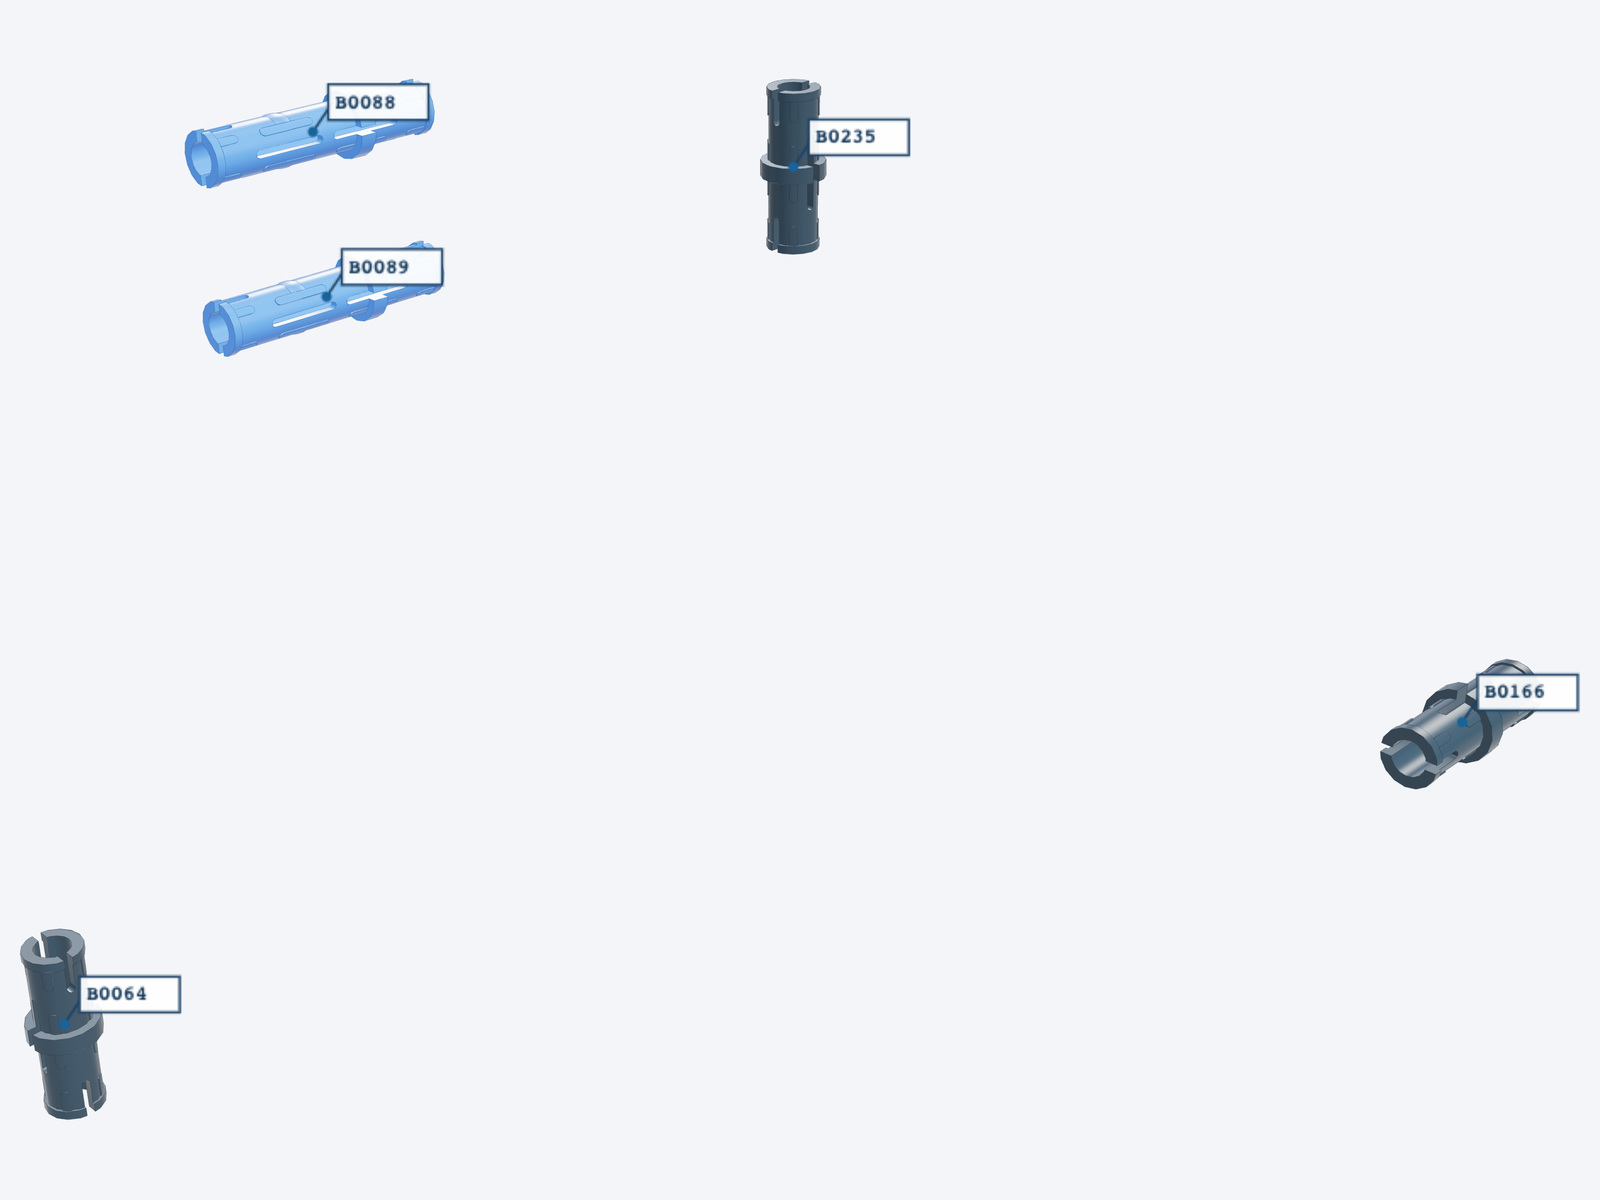
\includegraphics[width=.55\linewidth]{figures/ldraw/print/omr-42061-numbered.jpg}\end{center}
\begin{enumerate}
\item \textbf{color-1}. Identify the original color of B0088; numbered isolation is allowed.\par {\small \textit{Input:} Numbered visual input; source attributes are withheld from the model. \par\textit{Options:} A: Tan; B: Dark Bluish Grey; C: Rubber Black; D: Blue. \par\textit{Reference output:} D.}
\item \textbf{shape-match-1}. Ignoring color and pose, which numbered instance has the same LDraw part type as B0088?\par {\small \textit{Input:} Numbered visual input; source attributes are withheld from the model. \par\textit{Options:} A: B0089; B: B0064; C: B0166; D: B0235. \par\textit{Reference output:} A.}
\item \textbf{distance-1}. Using the supplied geometry bounding-box centers, which candidate is nearest to B0088?\par {\small \textit{Input:} Centers (mm): B0088 = (8, 92, 25.6); B0021 = (-8, 24.8, 76); B0194 = (8, 100, 129.6); B0203 = (39.9992, 48.8016, 56). \par\textit{Options:} A: B0194; B: B0203; C: B0021. \par\textit{Reference output:} B.}
\item \textbf{color-2}. Identify the original color of B0104; numbered isolation is allowed.\par {\small \textit{Input:} Numbered visual input; source attributes are withheld from the model. \par\textit{Options:} A: Reddish Brown; B: Light Bluish Grey; C: Red; D: Black. \par\textit{Reference output:} B.}
\item \textbf{shape-match-2}. Ignoring color and pose, which numbered instance has the same LDraw part type as B0104?\par {\small \textit{Input:} Numbered visual input; source attributes are withheld from the model. \par\textit{Options:} A: B0063; B: B0183; C: B0151; D: B0174. \par\textit{Reference output:} B.}
\item \textbf{distance-2}. Using the supplied geometry bounding-box centers, which candidate is nearest to B0104?\par {\small \textit{Input:} Centers (mm): B0104 = (8, 61.6, 6.4); B0252 = (40.0004, 88.9044, 48); B0204 = (39.9992, 48.8016, 88); B0134 = (-40, 50.381801, 52.818109). \par\textit{Options:} A: B0252; B: B0134; C: B0204. \par\textit{Reference output:} A.}
\item \textbf{interface-1}. Classify the supplied connector record for B0237 and B0236. This does not certify load capacity.\par {\small \textit{Input:} Record: family = axle; connector indices = 1, 0. \par\textit{Options:} A: ball; B: fixed; C: axle; D: hinge. \par\textit{Reference output:} C.}
\item \textbf{interface-2}. Classify the supplied connector record for B0260 and B0261. This does not certify load capacity.\par {\small \textit{Input:} Record: family = fixed; connector indices = 2, 0. \par\textit{Options:} A: ball; B: fixed; C: hinge; D: axle. \par\textit{Reference output:} B.}
\item \textbf{interface-3}. Classify the supplied connector record for B0210 and B0211. This does not certify load capacity.\par {\small \textit{Input:} Record: family = stud; connector indices = 2, 0. \par\textit{Options:} A: stud; B: axle; C: fixed; D: ball; E: hinge. \par\textit{Reference output:} A.}
\item \textbf{neighbors-1}. Select every candidate directly adjacent to B0130 in the supplied connector graph.\par {\small \textit{Input:} Unique undirected pairs: B0128 / B0130; B0130 / B0132. \par\textit{Options:} A: B0117; B: B0132; C: B0172; D: B0128. \par\textit{Reference output:} B, D.}
\item \textbf{graph-removal-1}. Delete B0130 and its incident edges from this local graph. How many connected components remain? Do not infer physical extractability.\par {\small \textit{Input:} Nodes: B0130, B0128, B0132, B0117, B0172. Unique undirected pairs: B0128 / B0130; B0130 / B0132. \par\textit{Options:} A: 3; B: 6; C: 5; D: 4. \par\textit{Reference output:} D.}
\item \textbf{neighbors-2}. Select every candidate directly adjacent to B0075 in the supplied connector graph.\par {\small \textit{Input:} Unique undirected pairs: B0075 / B0076; B0075 / B0079. \par\textit{Options:} A: B0076; B: B0067; C: B0026; D: B0079. \par\textit{Reference output:} A, D.}
\item \textbf{graph-removal-2}. Delete B0075 and its incident edges from this local graph. How many connected components remain? Do not infer physical extractability.\par {\small \textit{Input:} Nodes: B0075, B0079, B0076, B0067, B0026. Unique undirected pairs: B0075 / B0076; B0075 / B0079. \par\textit{Options:} A: 5; B: 6; C: 3; D: 4. \par\textit{Reference output:} D.}
\item \textbf{coverage-1}. Which numbered instance lacks a connector definition in the coverage record, so this audit cannot establish that it is floating?\par {\small \textit{Input:} Definition coverage: B0066 = unsupported; B0088 = supported; B0104 = supported; B0212 = supported. \par\textit{Options:} A: B0212; B: B0104; C: B0066; D: B0088. \par\textit{Reference output:} C.}
\item \textbf{evidence-limit-1}. Only source geometry, connector matching and mesh intersection audits are available. Without mass, friction, material or dynamic tests, is gravitational stability established?\par {\small \textit{Input:} Available evidence: Original CAD; Connector inference; Inset-mesh intersection candidates. \par\textit{Options:} A: Established; B: Not established by this evidence. \par\textit{Reference output:} B.}
\item \textbf{source-step-1}. At which expanded author step does B0041 first appear in the supplied source-step table? Source order is not a collision-free assembly proof.\par {\small \textit{Input:} Expanded author records: step 1: B0001; step 8: B0041. \par\textit{Options:} A: 10; B: 7; C: 8; D: 9. \par\textit{Reference output:} C.}
\item \textbf{source-step-2}. At which expanded author step does B0245 first appear in the supplied source-step table? Source order is not a collision-free assembly proof.\par {\small \textit{Input:} Expanded author records: step 1: B0001; step 42: B0245. \par\textit{Options:} A: 42; B: 44; C: 43; D: 41. \par\textit{Reference output:} A.}
\item \textbf{source-sequence-1}. Reveal the supplied source-step window in author order. Actions change visibility only, without simulating insertion trajectories.\par {\small \textit{Input:} Source window: step-1: B0001, B0002, B0003, B0004, B0005, B0006; step-2: B0007, B0008, B0009, B0010, B0011, B0012, B0013, B0014, B0015, B0016; step-3: B0017, B0018, B0019, B0020, B0021, B0022, B0023; step-4: B0024, B0025, B0026, B0027, B0028; step-5: B0029, B0030, B0031, B0032, B0033, B0034; step-6: B0035. Action budget: 6. \par\textit{Reference output:} step-1, step-2, step-3, step-4, step-5, step-6.}
\item \textbf{restore-instance-1}. The display copy hides B0088. Restore only that numbered instance, preserving all other instances and source poses.\par {\small \textit{Input:} Target: B0088. Action budget: 1. All other instances initially remain visible. \par\textit{Reference output:} restore-B0088.}
\item \textbf{restore-instance-2}. The display copy hides B0104. Restore only that numbered instance, preserving all other instances and source poses.\par {\small \textit{Input:} Target: B0104. Action budget: 1. All other instances initially remain visible. \par\textit{Reference output:} restore-B0104.}
\end{enumerate}
\clearpage
\section{31009: Small Cottage}
270 source instances; 20 tasks; D2 scale band.

\par\noindent Perspective, front, side and top views follow in reading order. Original source transforms are preserved.
\begin{center}
\includegraphics[width=.48\linewidth]{figures/ldraw/print/31009-iso.jpg}
\includegraphics[width=.48\linewidth]{figures/ldraw/print/31009-front.jpg}\\
\includegraphics[width=.48\linewidth]{figures/ldraw/print/31009-side.jpg}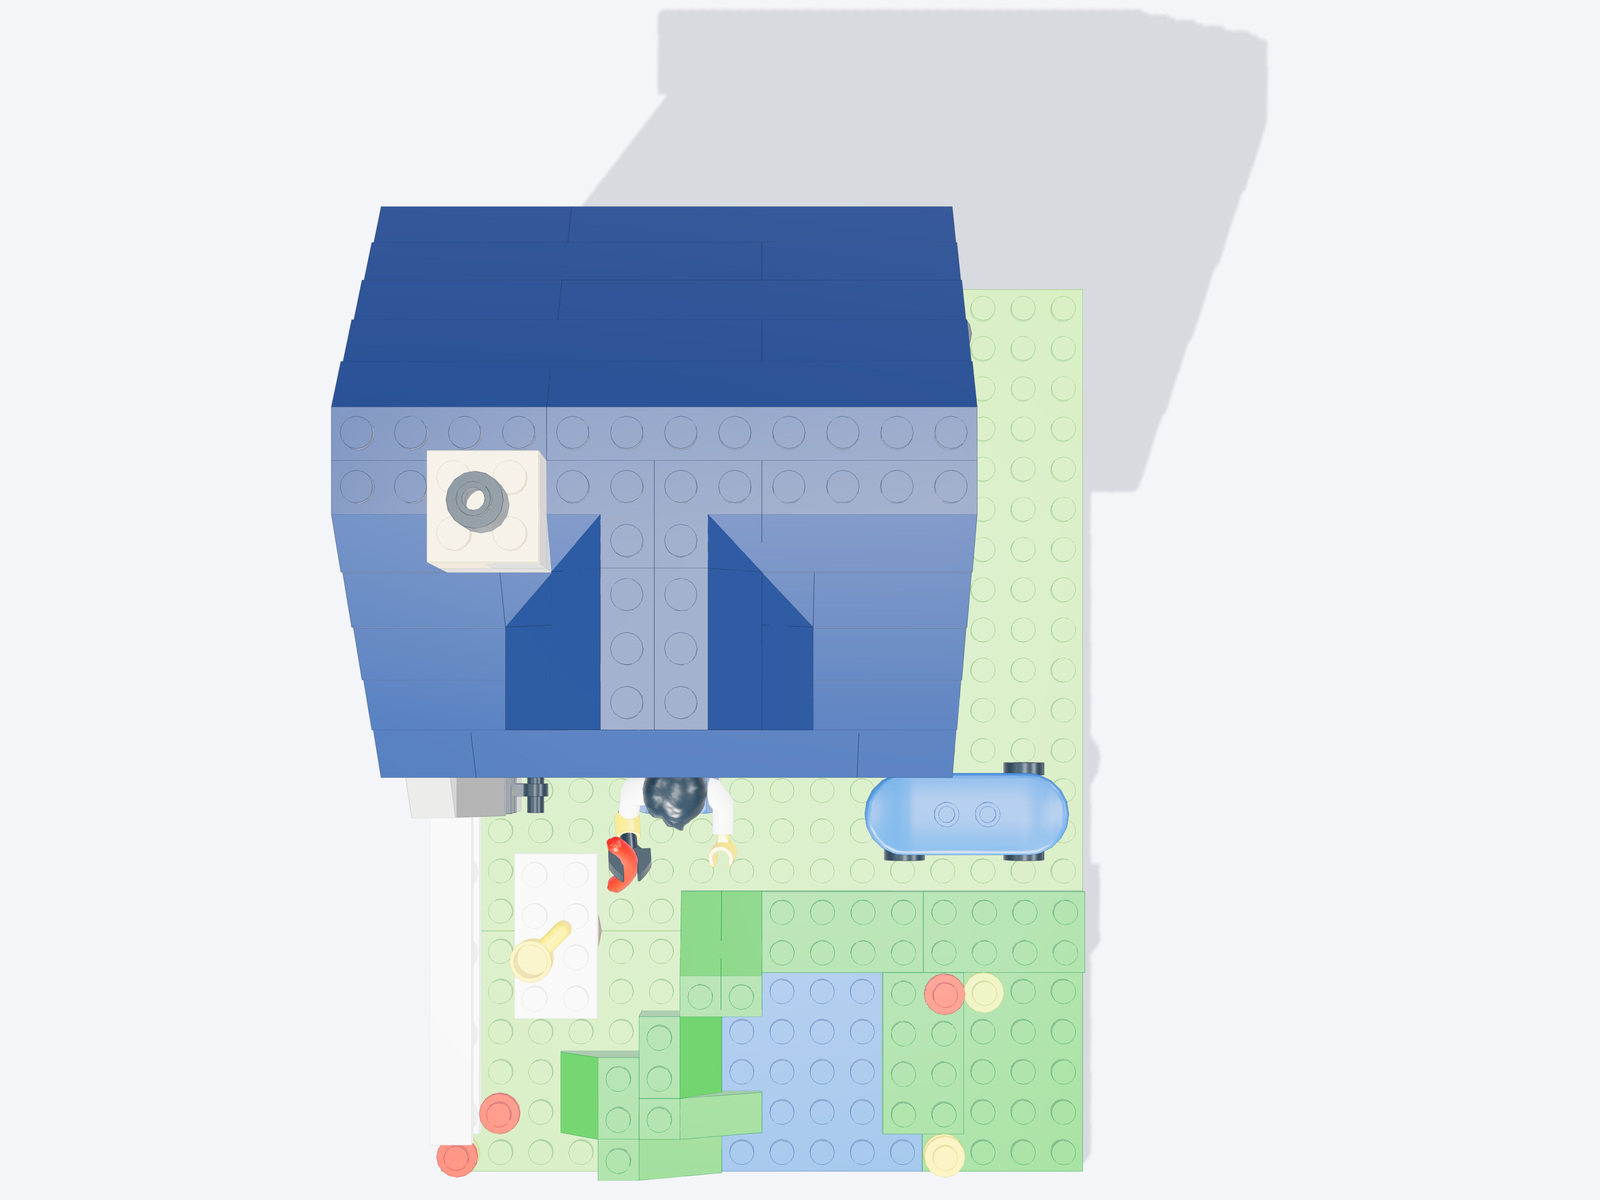
\includegraphics[width=.48\linewidth]{figures/ldraw/print/31009-top.jpg}\end{center}
\paragraph{Attribution.}Stefan Frenz [smf]. CC BY 2.0.\par\noindent\url{https://library.ldraw.org/omr/sets/1164}
\paragraph{Source lock.}\small\texttt{97b83517b0e843f8071ea3e4e80fbe0c}\\\texttt{7897685a7f476d3ba83161bb1185333d}\normalsize
\paragraph{Evidence coverage.}Connector definitions cover 97.04\% of instances. The audit reports 12 recognized-graph components and 0 intersection candidates without a recognized mating pair. 8 instances have no connector definition. These counts do not certify physical defects or gravitational stability.
\paragraph{Instructions.}79 expanded author steps.
\clearpage\subsection{Numbered visual input and complete question index}
Only relevant numbers are shown. The website can isolate any instance; public visual tasks provide their own numbered images. The following entries give every English prompt, all choice options, compact public evidence and the reference output. Raw repeated connector records and full action fact sets remain in the versioned JSON.
\begin{center}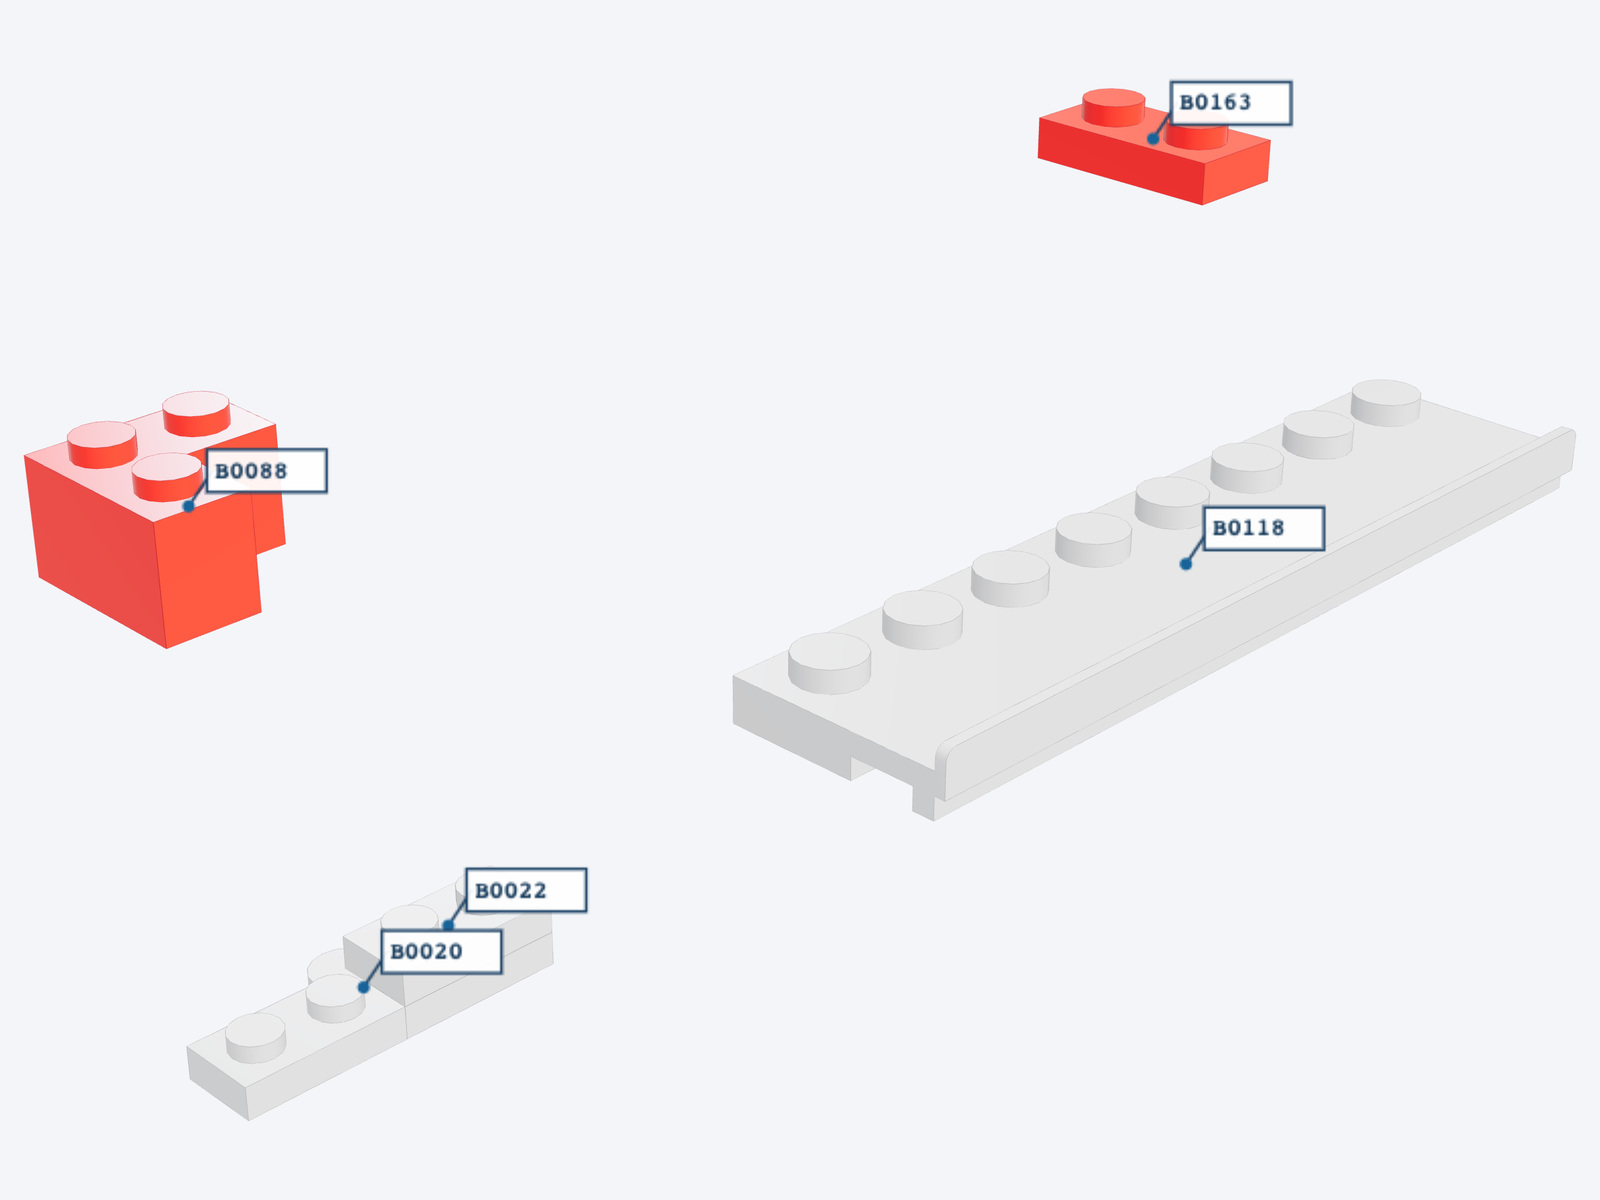
\includegraphics[width=.55\linewidth]{figures/ldraw/print/31009-numbered.jpg}\end{center}
\begin{enumerate}
\item \textbf{color-1}. Identify the original color of B0163; numbered isolation is allowed.\par {\small \textit{Input:} Numbered visual input; source attributes are withheld from the model. \par\textit{Options:} A: Medium Blue; B: Red; C: Light Bluish Grey; D: Trans Clear. \par\textit{Reference output:} B.}
\item \textbf{shape-match-1}. Ignoring color and pose, which numbered instance has the same LDraw part type as B0163?\par {\small \textit{Input:} Numbered visual input; source attributes are withheld from the model. \par\textit{Options:} A: B0020; B: B0088; C: B0022; D: B0118. \par\textit{Reference output:} C.}
\item \textbf{distance-1}. Using the supplied geometry bounding-box centers, which candidate is nearest to B0163?\par {\small \textit{Input:} Centers (mm): B0163 = (4, 79.2, -16); B0200 = (-32, 96.8, 12); B0063 = (-68, 40.8, 0); B0145 = (12, 15.2, -52). \par\textit{Options:} A: B0063; B: B0145; C: B0200. \par\textit{Reference output:} C.}
\item \textbf{color-2}. Identify the original color of B0262; numbered isolation is allowed.\par {\small \textit{Input:} Numbered visual input; source attributes are withheld from the model. \par\textit{Options:} A: Light Bluish Grey; B: Trans Clear; C: Blue; D: Dark Blue. \par\textit{Reference output:} C.}
\item \textbf{distance-2}. Using the supplied geometry bounding-box centers, which candidate is nearest to B0262?\par {\small \textit{Input:} Centers (mm): B0262 = (-32, 28, 35.6); B0099 = (12, 67.12, -28); B0085 = (-72, 56.8, 16); B0235 = (-76, 12, 100). \par\textit{Options:} A: B0099; B: B0085; C: B0235. \par\textit{Reference output:} B.}
\item \textbf{interface-1}. Classify the supplied connector record for B0263 and B0262. This does not certify load capacity.\par {\small \textit{Input:} Record: family = axle; connector indices = 1, 0. \par\textit{Options:} A: ball; B: hinge; C: axle; D: fixed. \par\textit{Reference output:} C.}
\item \textbf{interface-2}. Classify the supplied connector record for B0261 and B0262. This does not certify load capacity.\par {\small \textit{Input:} Record: family = fixed; connector indices = 1, 1. \par\textit{Options:} A: ball; B: hinge; C: axle; D: fixed. \par\textit{Reference output:} D.}
\item \textbf{interface-3}. Classify the supplied connector record for B0259 and B0258. This does not certify load capacity.\par {\small \textit{Input:} Record: family = hinge; connector indices = 1, 2. \par\textit{Options:} A: fixed; B: ball; C: axle; D: hinge. \par\textit{Reference output:} D.}
\item \textbf{interface-4}. Classify the supplied connector record for B0064 and B0074. This does not certify load capacity.\par {\small \textit{Input:} Record: family = stud; connector indices = 5, 0. \par\textit{Options:} A: stud; B: axle; C: fixed; D: ball; E: hinge. \par\textit{Reference output:} A.}
\item \textbf{neighbors-1}. Select every candidate directly adjacent to B0048 in the supplied connector graph.\par {\small \textit{Input:} Unique undirected pairs: B0033 / B0048; B0048 / B0057. \par\textit{Options:} A: B0057; B: B0139; C: B0165; D: B0033. \par\textit{Reference output:} A, D.}
\item \textbf{graph-removal-1}. Delete B0048 and its incident edges from this local graph. How many connected components remain? Do not infer physical extractability.\par {\small \textit{Input:} Nodes: B0048, B0033, B0057, B0165, B0139. Unique undirected pairs: B0033 / B0048; B0048 / B0057. \par\textit{Options:} A: 6; B: 3; C: 4; D: 5. \par\textit{Reference output:} C.}
\item \textbf{neighbors-2}. Select every candidate directly adjacent to B0202 in the supplied connector graph.\par {\small \textit{Input:} Unique undirected pairs: B0184 / B0202; B0185 / B0202; B0186 / B0202; B0193 / B0202; B0202 / B0217; B0202 / B0218. \par\textit{Options:} A: B0218; B: B0195; C: B0184; D: B0185; E: B0217; F: B0193; G: B0216; H: B0186. \par\textit{Reference output:} A, C, D, E, F, H.}
\item \textbf{graph-removal-2}. Delete B0202 and its incident edges from this local graph. How many connected components remain? Do not infer physical extractability.\par {\small \textit{Input:} Nodes: B0202, B0217, B0218, B0186, B0184, B0193, B0185, B0195, B0216. Unique undirected pairs: B0184 / B0202; B0185 / B0202; B0186 / B0202; B0193 / B0202; B0202 / B0217; B0202 / B0218. \par\textit{Options:} A: 8; B: 7; C: 10; D: 9. \par\textit{Reference output:} A.}
\item \textbf{coverage-1}. Which numbered instance lacks a connector definition in the coverage record, so this audit cannot establish that it is floating?\par {\small \textit{Input:} Definition coverage: B0068 = unsupported; B0163 = supported; B0262 = supported; B0016 = supported. \par\textit{Options:} A: B0163; B: B0068; C: B0016; D: B0262. \par\textit{Reference output:} B.}
\item \textbf{evidence-limit-1}. Only source geometry, connector matching and mesh intersection audits are available. Without mass, friction, material or dynamic tests, is gravitational stability established?\par {\small \textit{Input:} Available evidence: Original CAD; Connector inference; Inset-mesh intersection candidates. \par\textit{Options:} A: Not established by this evidence; B: Established. \par\textit{Reference output:} A.}
\item \textbf{source-step-1}. At which expanded author step does B0006 first appear in the supplied source-step table? Source order is not a collision-free assembly proof.\par {\small \textit{Input:} Expanded author records: step 1: B0001; step 3: B0006. \par\textit{Options:} A: 4; B: 3; C: 2; D: 5. \par\textit{Reference output:} B.}
\item \textbf{source-step-2}. At which expanded author step does B0107 first appear in the supplied source-step table? Source order is not a collision-free assembly proof.\par {\small \textit{Input:} Expanded author records: step 1: B0001; step 32: B0107. \par\textit{Options:} A: 33; B: 31; C: 32; D: 34. \par\textit{Reference output:} C.}
\item \textbf{source-sequence-1}. Reveal the supplied source-step window in author order. Actions change visibility only, without simulating insertion trajectories.\par {\small \textit{Input:} Source window: step-1: B0001, B0002; step-2: B0003, B0004, B0005; step-3: B0006, B0007, B0008; step-4: B0009, B0010; step-5: B0011, B0012, B0013, B0014, B0015, B0016; step-6: B0017, B0018, B0019, B0020, B0021, B0022. Action budget: 6. \par\textit{Reference output:} step-1, step-2, step-3, step-4, step-5, step-6.}
\item \textbf{restore-instance-1}. The display copy hides B0163. Restore only that numbered instance, preserving all other instances and source poses.\par {\small \textit{Input:} Target: B0163. Action budget: 1. All other instances initially remain visible. \par\textit{Reference output:} restore-B0163.}
\item \textbf{restore-instance-2}. The display copy hides B0262. Restore only that numbered instance, preserving all other instances and source poses.\par {\small \textit{Input:} Target: B0262. Action budget: 1. All other instances initially remain visible. \par\textit{Reference output:} restore-B0262.}
\end{enumerate}
\clearpage
\section{5867: Super Speedster}
278 source instances; 18 tasks; D2 scale band.

\par\noindent Perspective, front, side and top views follow in reading order. Original source transforms are preserved.
\begin{center}
\includegraphics[width=.48\linewidth]{figures/ldraw/print/5867-iso.jpg}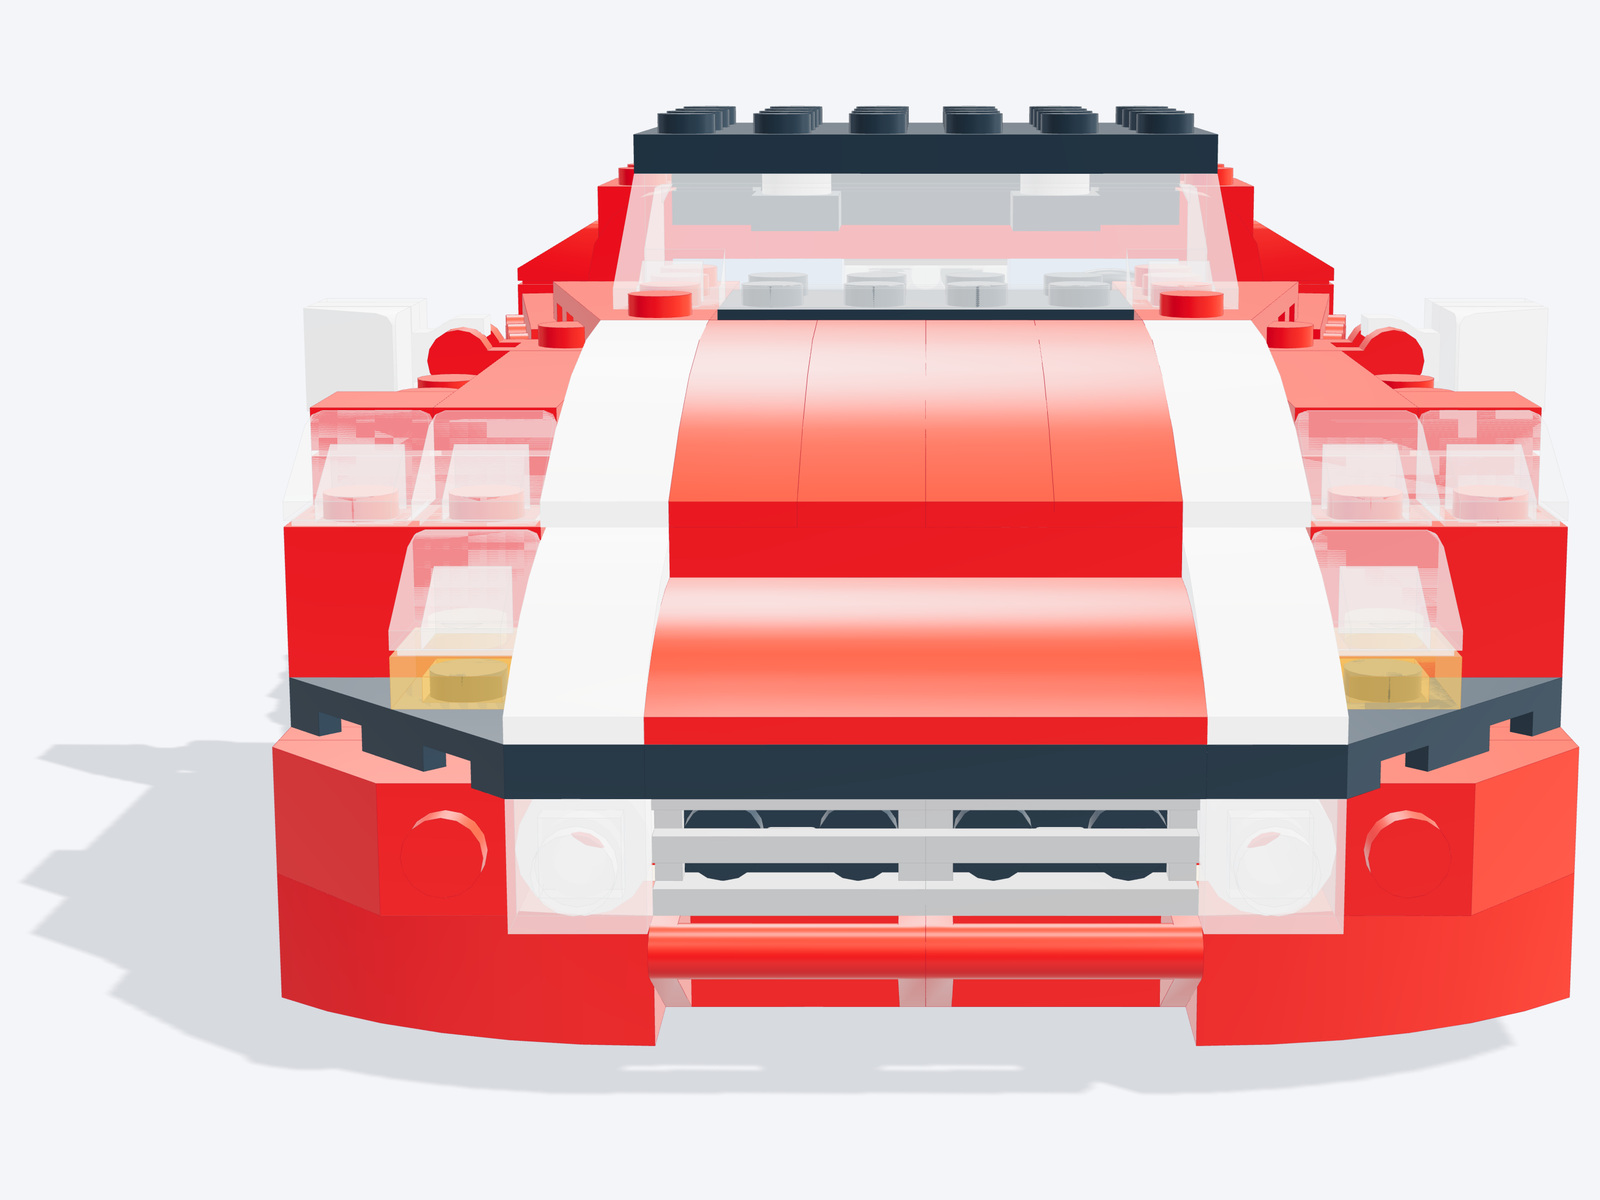
\includegraphics[width=.48\linewidth]{figures/ldraw/print/5867-front.jpg}\\
\includegraphics[width=.48\linewidth]{figures/ldraw/print/5867-side.jpg}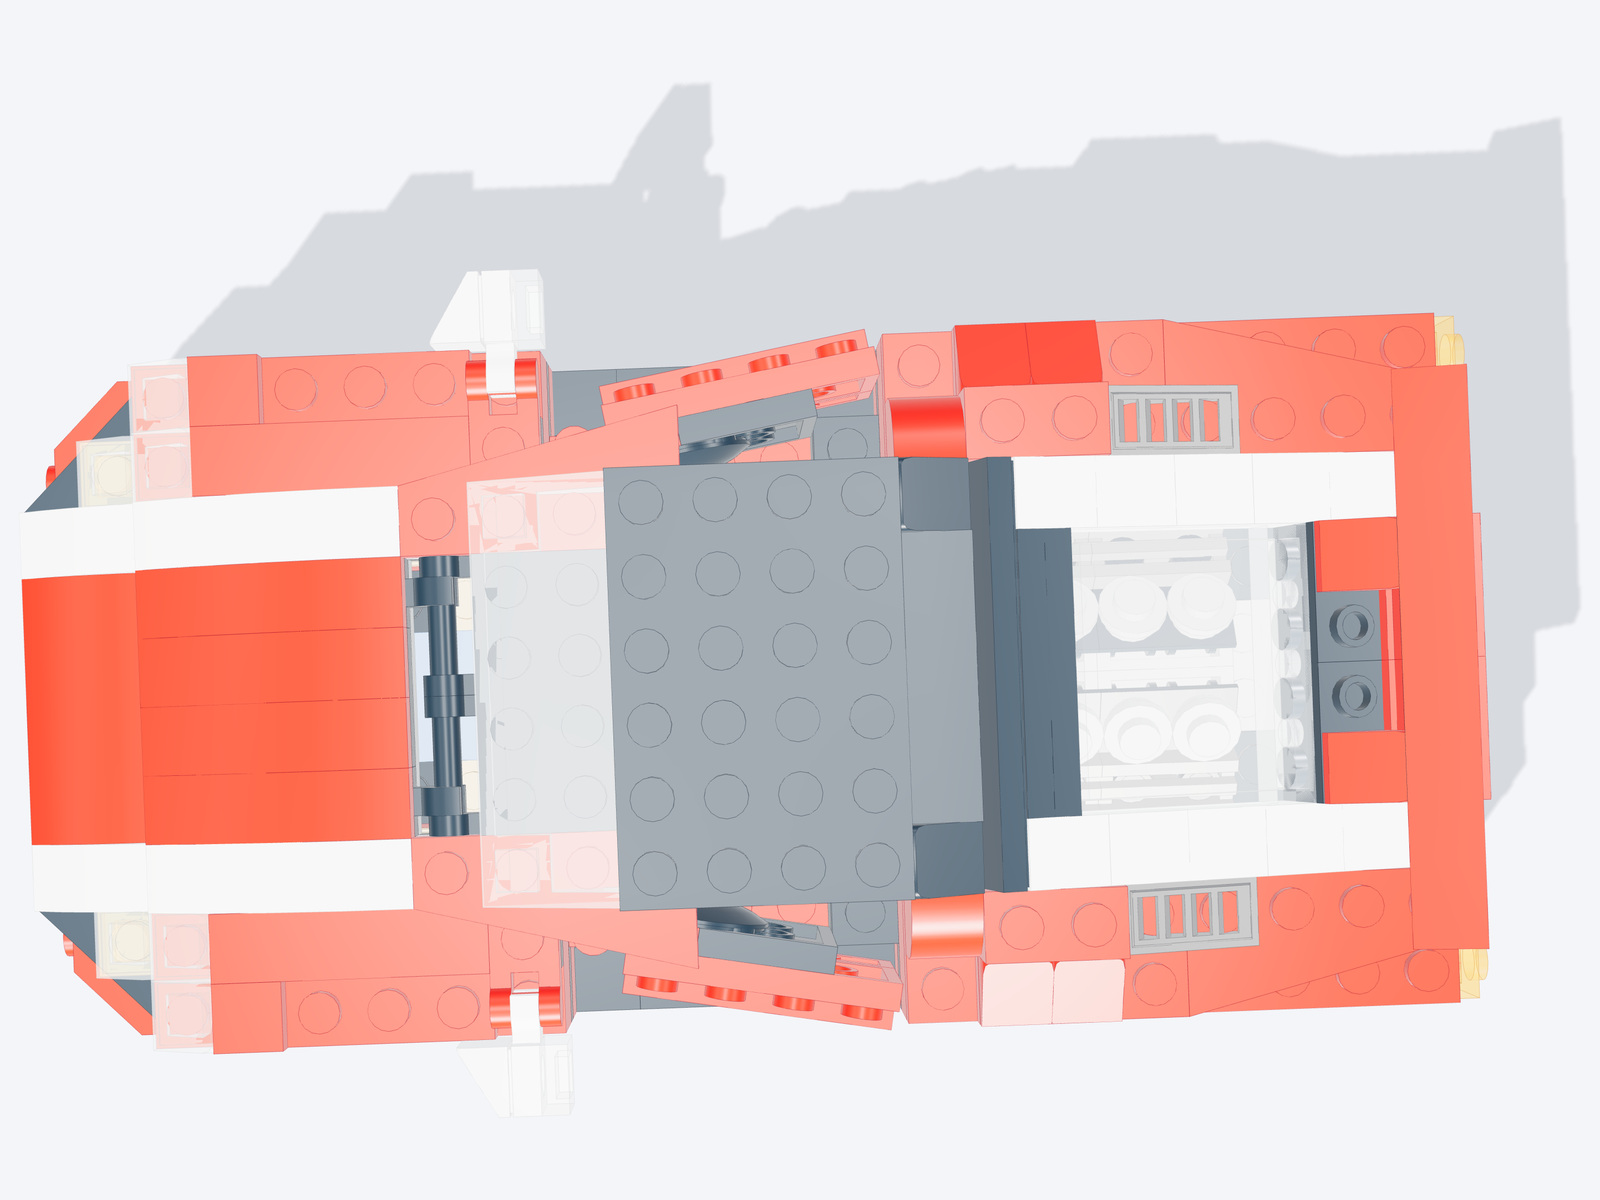
\includegraphics[width=.48\linewidth]{figures/ldraw/print/5867-top.jpg}\end{center}
\paragraph{Attribution.}Takeshi Takahashi [RainbowDolphin]. CC BY 2.0.\par\noindent\url{https://library.ldraw.org/omr/sets/1431}
\paragraph{Source lock.}\small\texttt{48082e34b40a6ed5bbf2edabe9d0deb3}\\\texttt{13fac7c20b1128970ba73f722b70216d}\normalsize
\paragraph{Evidence coverage.}Connector definitions cover 99.64\% of instances. The audit reports 2 recognized-graph components and 0 intersection candidates without a recognized mating pair. 1 instances have no connector definition. These counts do not certify physical defects or gravitational stability.
\paragraph{Instructions.}No author STEP replay or source-order question is provided.
\clearpage\subsection{Numbered visual input and complete question index}
Only relevant numbers are shown. The website can isolate any instance; public visual tasks provide their own numbered images. The following entries give every English prompt, all choice options, compact public evidence and the reference output. Raw repeated connector records and full action fact sets remain in the versioned JSON.
\begin{center}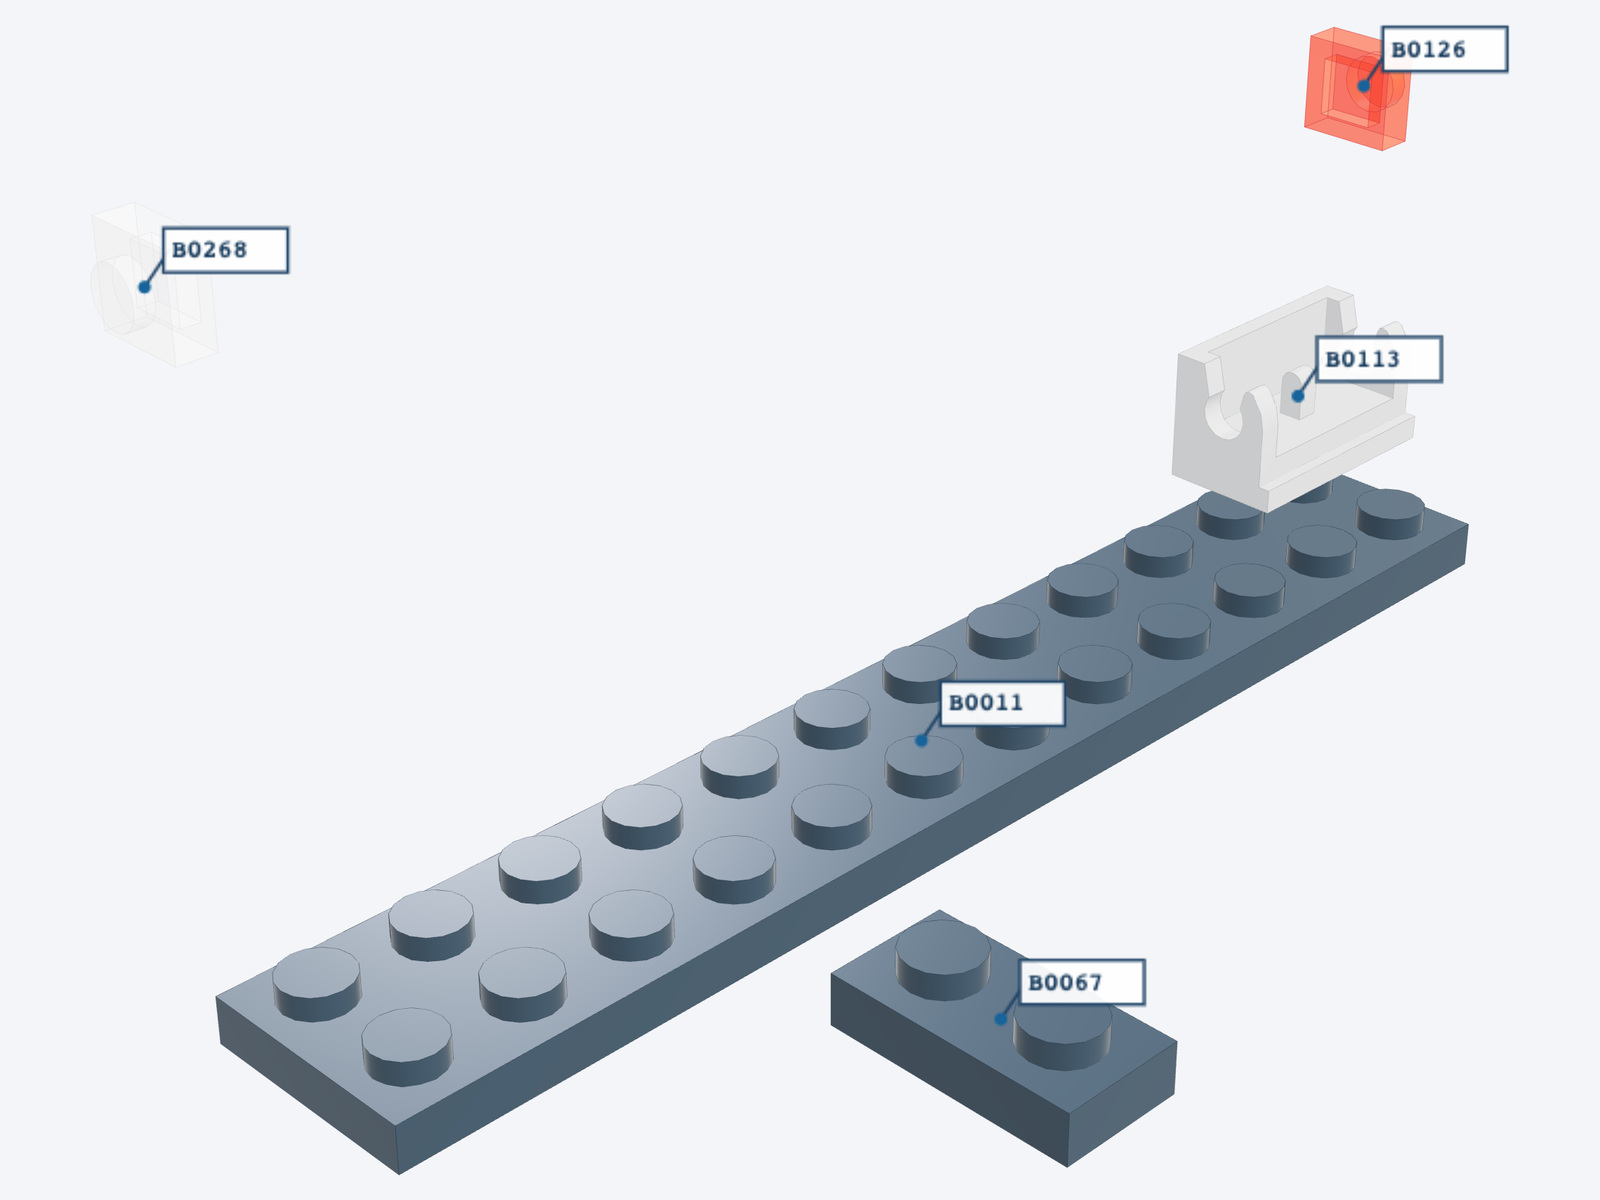
\includegraphics[width=.55\linewidth]{figures/ldraw/print/5867-numbered.jpg}\end{center}
\begin{enumerate}
\item \textbf{color-1}. Identify the original color of B0126; numbered isolation is allowed.\par {\small \textit{Input:} Numbered visual input; source attributes are withheld from the model. \par\textit{Options:} A: Light Bluish Grey; B: White; C: Red; D: Trans Red. \par\textit{Reference output:} D.}
\item \textbf{shape-match-1}. Ignoring color and pose, which numbered instance has the same LDraw part type as B0126?\par {\small \textit{Input:} Numbered visual input; source attributes are withheld from the model. \par\textit{Options:} A: B0011; B: B0067; C: B0113; D: B0268. \par\textit{Reference output:} D.}
\item \textbf{distance-1}. Using the supplied geometry bounding-box centers, which candidate is nearest to B0126?\par {\small \textit{Input:} Centers (mm): B0126 = (82.4, 21.6, -28); B0258 = (-56, 30.4, 4); B0127 = (82.4, 21.6, 28); B0048 = (-80.8, 8.8, 20). \par\textit{Options:} A: B0258; B: B0048; C: B0127. \par\textit{Reference output:} C.}
\item \textbf{color-2}. Identify the original color of B0232; numbered isolation is allowed.\par {\small \textit{Input:} Numbered visual input; source attributes are withheld from the model. \par\textit{Options:} A: Light Bluish Grey; B: Black; C: Medium Blue; D: Dark Bluish Grey. \par\textit{Reference output:} B.}
\item \textbf{shape-match-2}. Ignoring color and pose, which numbered instance has the same LDraw part type as B0232?\par {\small \textit{Input:} Numbered visual input; source attributes are withheld from the model. \par\textit{Options:} A: B0238; B: B0138; C: B0086; D: B0114. \par\textit{Reference output:} A.}
\item \textbf{distance-2}. Using the supplied geometry bounding-box centers, which candidate is nearest to B0232?\par {\small \textit{Input:} Centers (mm): B0232 = (-7.648536, 24, 27.340845); B0205 = (-32, 21.6, -32); B0020 = (16, 8.8, -16); B0079 = (78.32, 0.8, 4). \par\textit{Options:} A: B0020; B: B0205; C: B0079. \par\textit{Reference output:} A.}
\item \textbf{interface-1}. Classify the supplied connector record for B0272 and B0017. This does not certify load capacity.\par {\small \textit{Input:} Record: family = axle; connector indices = 0, 1. \par\textit{Options:} A: hinge; B: axle; C: ball; D: fixed. \par\textit{Reference output:} B.}
\item \textbf{interface-2}. Classify the supplied connector record for B0271 and B0275. This does not certify load capacity.\par {\small \textit{Input:} Record: family = fixed; connector indices = 2, 0. \par\textit{Options:} A: ball; B: fixed; C: axle; D: hinge. \par\textit{Reference output:} B.}
\item \textbf{interface-3}. Classify the supplied connector record for B0109 and B0108. This does not certify load capacity.\par {\small \textit{Input:} Record: family = hinge; connector indices = 6, 2. \par\textit{Options:} A: fixed; B: hinge; C: ball; D: axle. \par\textit{Reference output:} B.}
\item \textbf{interface-4}. Classify the supplied connector record for B0011 and B0033. This does not certify load capacity.\par {\small \textit{Input:} Record: family = stud; connector indices = 38, 3. \par\textit{Options:} A: hinge; B: fixed; C: stud; D: axle; E: ball. \par\textit{Reference output:} C.}
\item \textbf{neighbors-1}. Select every candidate directly adjacent to B0202 in the supplied connector graph.\par {\small \textit{Input:} Unique undirected pairs: B0069 / B0202; B0202 / B0215; B0202 / B0244; B0202 / B0245. \par\textit{Options:} A: B0244; B: B0215; C: B0056; D: B0245; E: B0069; F: B0021. \par\textit{Reference output:} A, B, D, E.}
\item \textbf{graph-removal-1}. Delete B0202 and its incident edges from this local graph. How many connected components remain? Do not infer physical extractability.\par {\small \textit{Input:} Nodes: B0202, B0244, B0245, B0215, B0069, B0056, B0021. Unique undirected pairs: B0069 / B0202; B0202 / B0215; B0202 / B0244; B0202 / B0245. \par\textit{Options:} A: 5; B: 6; C: 7; D: 8. \par\textit{Reference output:} B.}
\item \textbf{neighbors-2}. Select every candidate directly adjacent to B0193 in the supplied connector graph.\par {\small \textit{Input:} Unique undirected pairs: B0187 / B0193; B0193 / B0196; B0193 / B0228. \par\textit{Options:} A: B0228; B: B0196; C: B0031; D: B0187; E: B0197. \par\textit{Reference output:} A, B, D.}
\item \textbf{graph-removal-2}. Delete B0193 and its incident edges from this local graph. How many connected components remain? Do not infer physical extractability.\par {\small \textit{Input:} Nodes: B0193, B0196, B0187, B0228, B0197, B0031. Unique undirected pairs: B0187 / B0193; B0193 / B0196; B0193 / B0228. \par\textit{Options:} A: 6; B: 5; C: 7; D: 4. \par\textit{Reference output:} B.}
\item \textbf{coverage-1}. Which numbered instance lacks a connector definition in the coverage record, so this audit cannot establish that it is floating?\par {\small \textit{Input:} Definition coverage: B0194 = unsupported; B0126 = supported; B0232 = supported; B0109 = supported. \par\textit{Options:} A: B0194; B: B0109; C: B0126; D: B0232. \par\textit{Reference output:} A.}
\item \textbf{evidence-limit-1}. Only source geometry, connector matching and mesh intersection audits are available. Without mass, friction, material or dynamic tests, is gravitational stability established?\par {\small \textit{Input:} Available evidence: Original CAD; Connector inference; Inset-mesh intersection candidates. \par\textit{Options:} A: Established; B: Not established by this evidence. \par\textit{Reference output:} B.}
\item \textbf{restore-instance-1}. The display copy hides B0126. Restore only that numbered instance, preserving all other instances and source poses.\par {\small \textit{Input:} Target: B0126. Action budget: 1. All other instances initially remain visible. \par\textit{Reference output:} restore-B0126.}
\item \textbf{restore-instance-2}. The display copy hides B0232. Restore only that numbered instance, preserving all other instances and source poses.\par {\small \textit{Input:} Target: B0232. Action budget: 1. All other instances initially remain visible. \par\textit{Reference output:} restore-B0232.}
\end{enumerate}
\clearpage
\section{10128: Train Level Crossing}
336 source instances; 21 tasks; D2 scale band.

\par\noindent Perspective, front, side and top views follow in reading order. Original source transforms are preserved.
\begin{center}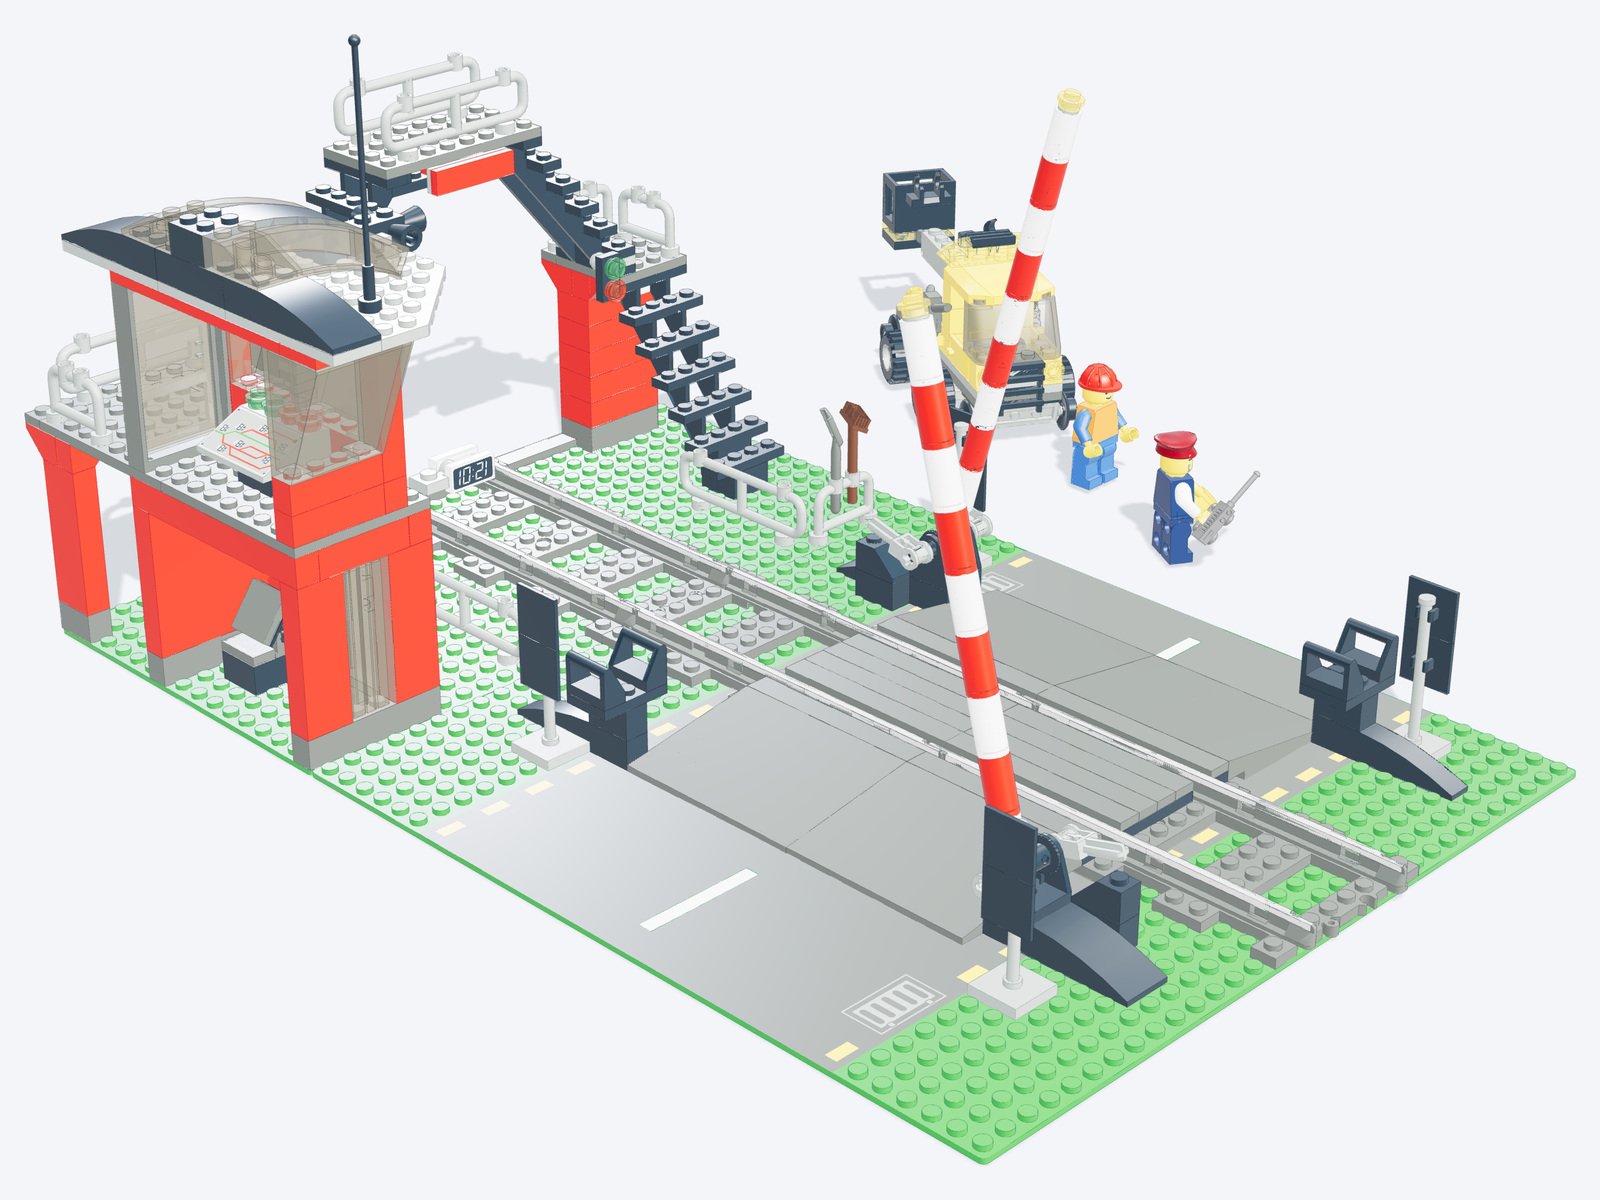
\includegraphics[width=.48\linewidth]{figures/ldraw/print/10128-iso.jpg}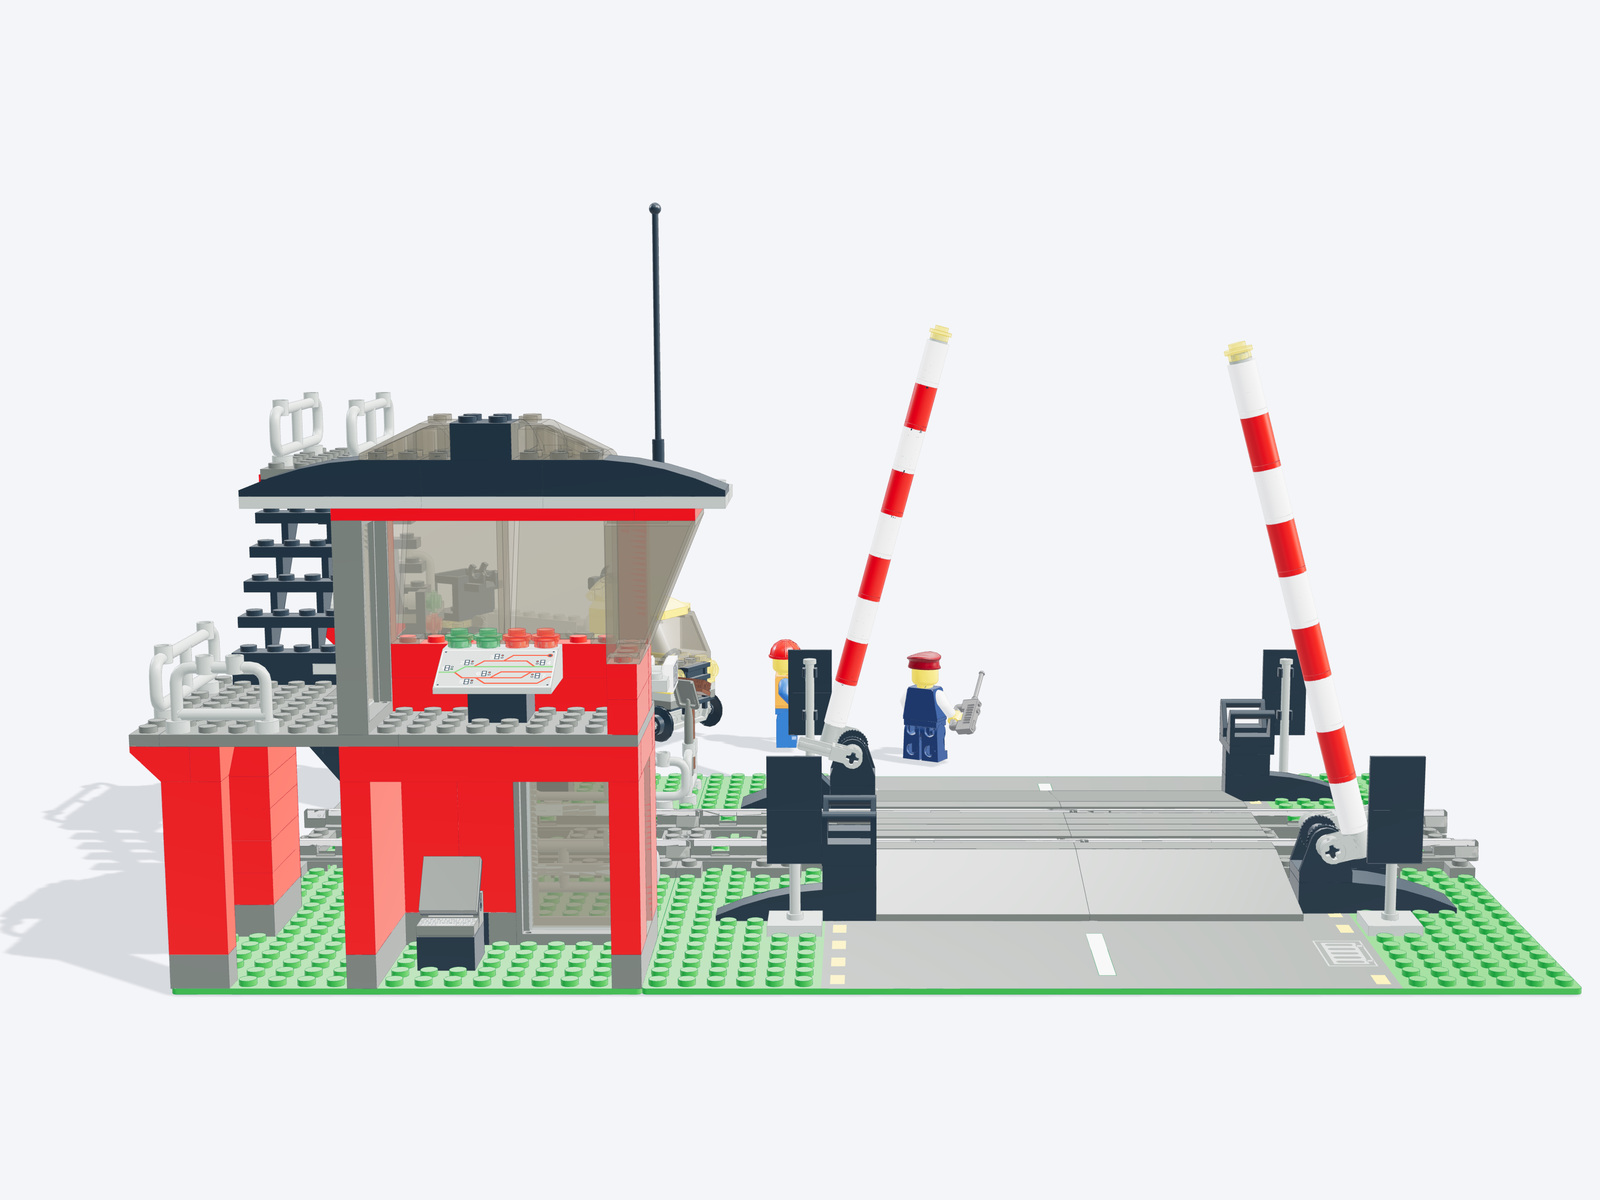
\includegraphics[width=.48\linewidth]{figures/ldraw/print/10128-front.jpg}\\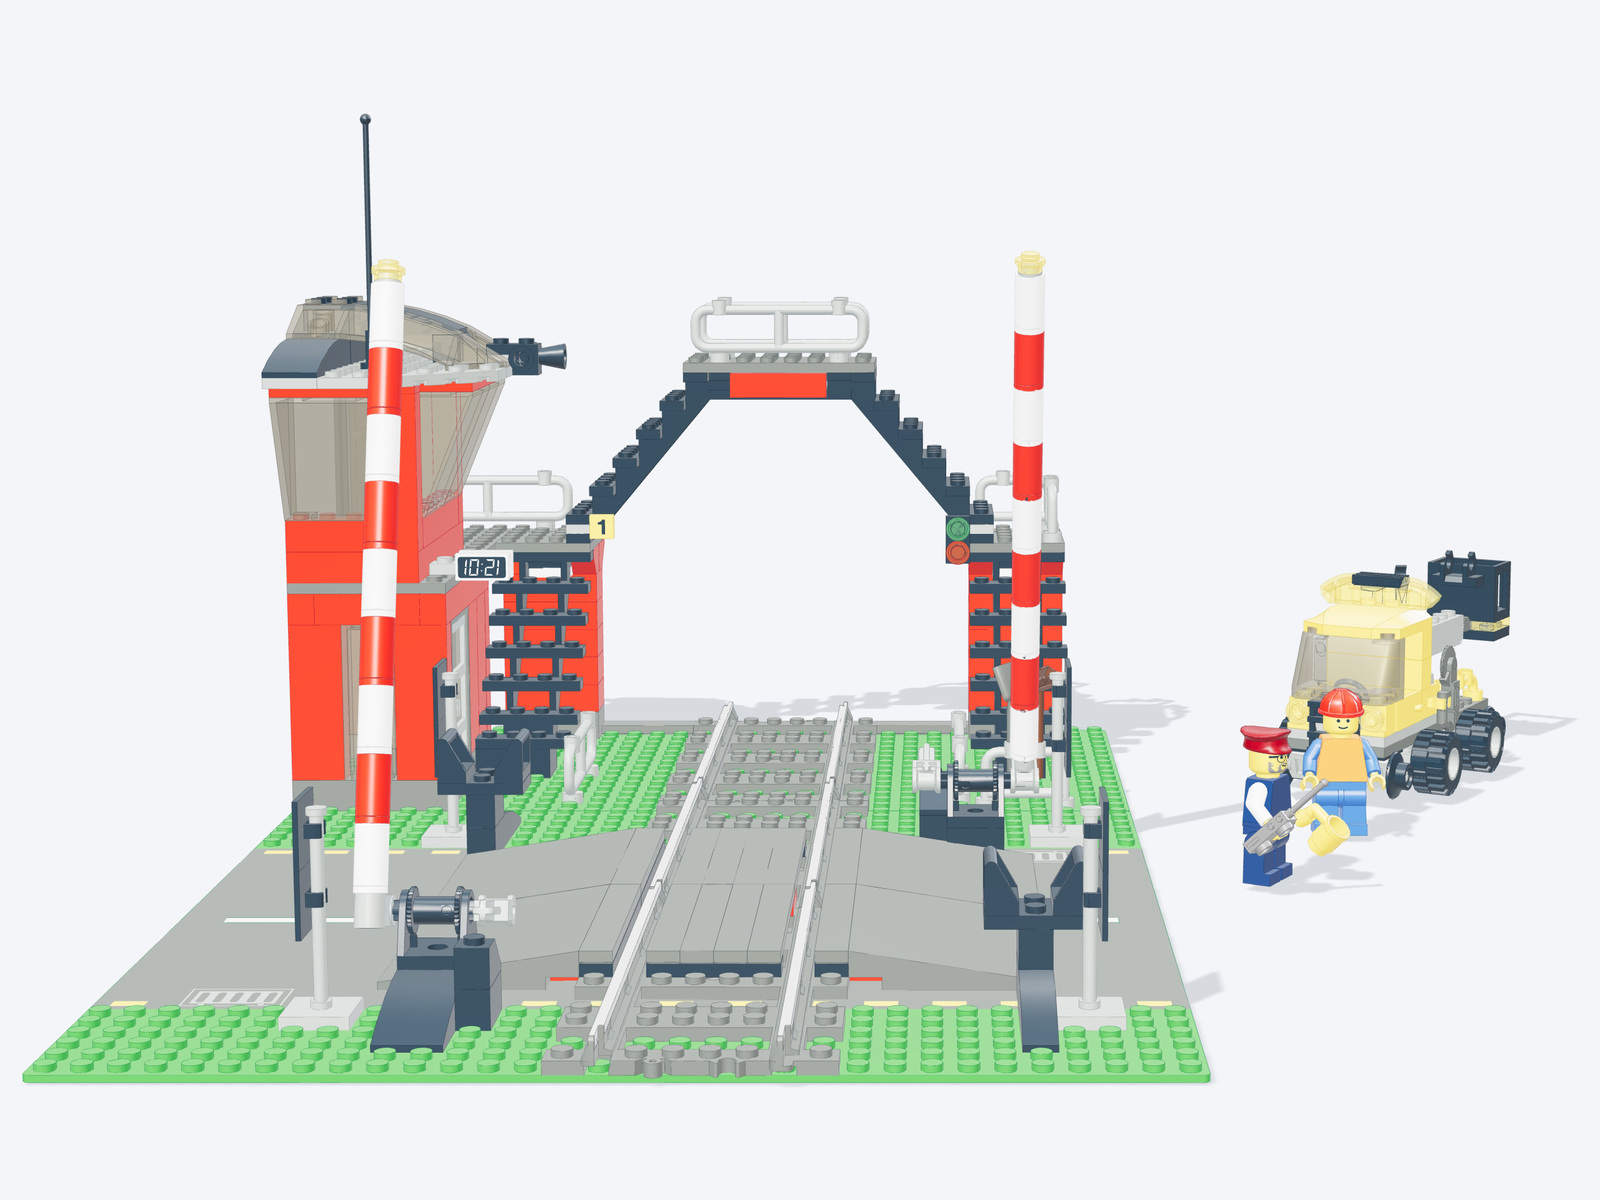
\includegraphics[width=.48\linewidth]{figures/ldraw/print/10128-side.jpg}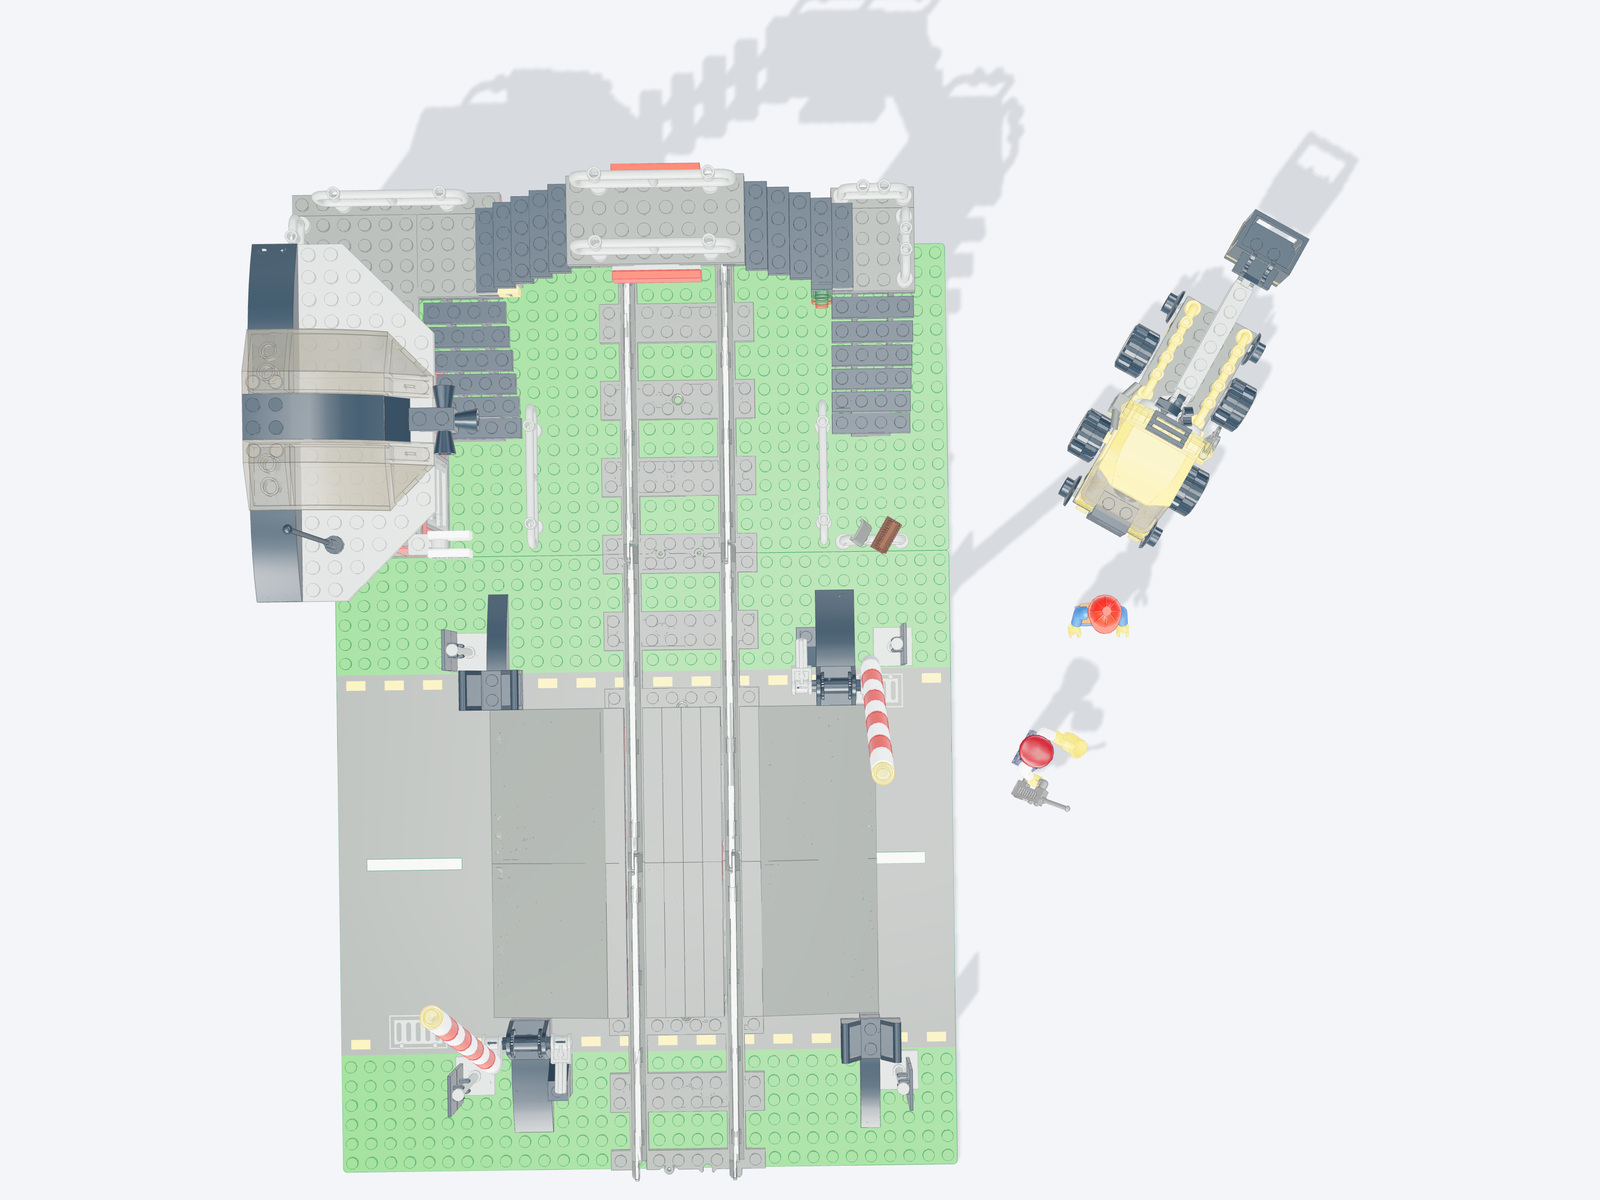
\includegraphics[width=.48\linewidth]{figures/ldraw/print/10128-top.jpg}\end{center}
\paragraph{Attribution.}Robert Paciorek [bercik]. CC BY 2.0.\par\noindent\url{https://library.ldraw.org/omr/sets/864}
\paragraph{Source lock.}\small\texttt{7928f4e259455ec49cc02c62acb1653f}\\\texttt{7a002824c789f099845936d0a2e8a0b9}\normalsize
\paragraph{Evidence coverage.}Connector definitions cover 99.40\% of instances. The audit reports 11 recognized-graph components and 1 intersection candidates without a recognized mating pair. 2 instances have no connector definition. These counts do not certify physical defects or gravitational stability.
\paragraph{Instructions.}87 expanded author steps.
\clearpage\subsection{Numbered visual input and complete question index}
Only relevant numbers are shown. The website can isolate any instance; public visual tasks provide their own numbered images. The following entries give every English prompt, all choice options, compact public evidence and the reference output. Raw repeated connector records and full action fact sets remain in the versioned JSON.
\begin{center}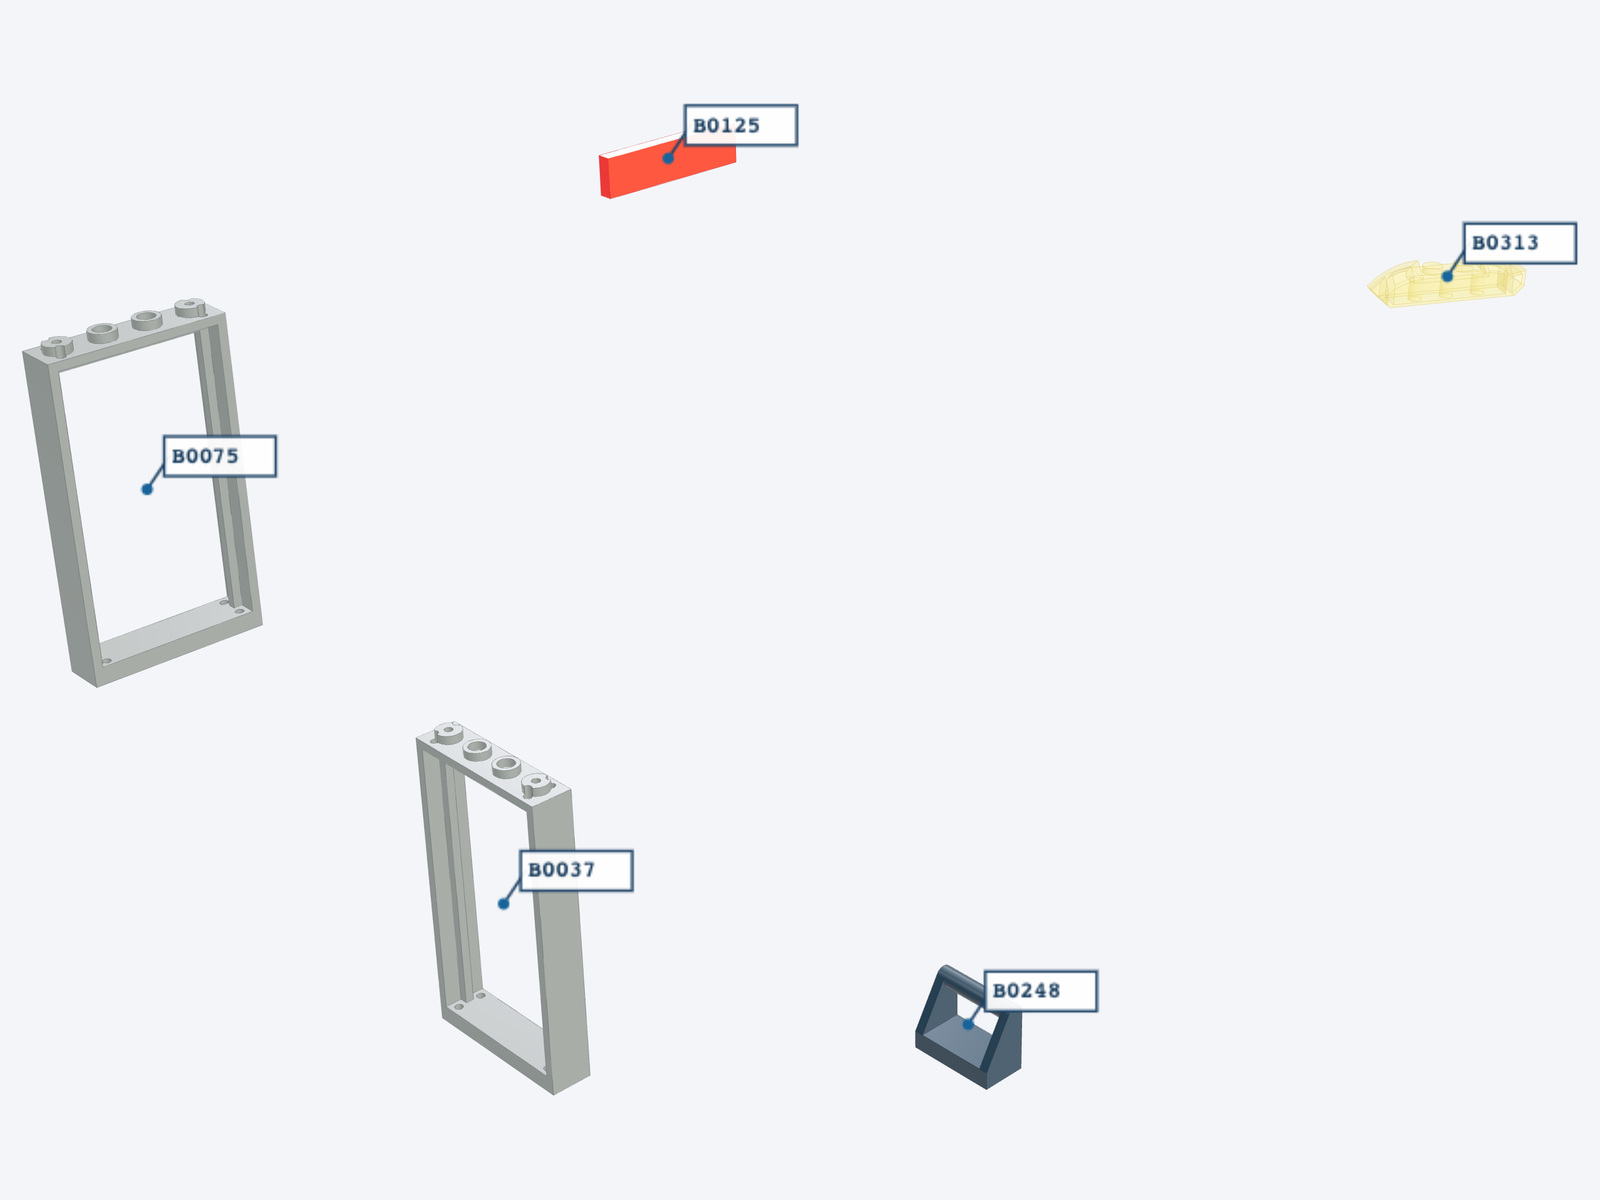
\includegraphics[width=.55\linewidth]{figures/ldraw/print/10128-numbered.jpg}\end{center}
\begin{enumerate}
\item \textbf{color-1}. Identify the original color of B0075; numbered isolation is allowed.\par {\small \textit{Input:} Numbered visual input; source attributes are withheld from the model. \par\textit{Options:} A: Dark Blue; B: Blue; C: Trans Brown; D: Dark Grey. \par\textit{Reference output:} D.}
\item \textbf{shape-match-1}. Ignoring color and pose, which numbered instance has the same LDraw part type as B0075?\par {\small \textit{Input:} Numbered visual input; source attributes are withheld from the model. \par\textit{Options:} A: B0313; B: B0248; C: B0037; D: B0125. \par\textit{Reference output:} C.}
\item \textbf{distance-1}. Using the supplied geometry bounding-box centers, which candidate is nearest to B0075?\par {\small \textit{Input:} Centers (mm): B0075 = (-72, 100, -60); B0105 = (-80, 133.6, 16); B0310 = (226.2552, 10.4, -29.7924); B0031 = (-44, 5.6, -28). \par\textit{Options:} A: B0310; B: B0105; C: B0031. \par\textit{Reference output:} B.}
\item \textbf{color-2}. Identify the original color of B0129; numbered isolation is allowed.\par {\small \textit{Input:} Numbered visual input; source attributes are withheld from the model. \par\textit{Options:} A: Light Grey; B: Dark Red; C: Trans Red; D: Green. \par\textit{Reference output:} A.}
\item \textbf{shape-match-2}. Ignoring color and pose, which numbered instance has the same LDraw part type as B0129?\par {\small \textit{Input:} Numbered visual input; source attributes are withheld from the model. \par\textit{Options:} A: B0144; B: B0074; C: B0145; D: B0161. \par\textit{Reference output:} B.}
\item \textbf{distance-2}. Using the supplied geometry bounding-box centers, which candidate is nearest to B0129?\par {\small \textit{Input:} Centers (mm): B0129 = (56, 141.6, -108); B0141 = (24, 2.4, 96); B0082 = (120.4, 76, -84); B0095 = (-52, 104.8, 12). \par\textit{Options:} A: B0082; B: B0141; C: B0095. \par\textit{Reference output:} A.}
\item \textbf{interface-1}. Classify the supplied connector record for B0260 and B0251. This does not certify load capacity.\par {\small \textit{Input:} Record: family = axle; connector indices = 1, 0. \par\textit{Options:} A: hinge; B: axle; C: fixed; D: ball. \par\textit{Reference output:} B.}
\item \textbf{interface-2}. Classify the supplied connector record for B0327 and B0326. This does not certify load capacity.\par {\small \textit{Input:} Record: family = fixed; connector indices = 0, 2. \par\textit{Options:} A: axle; B: ball; C: fixed; D: hinge. \par\textit{Reference output:} C.}
\item \textbf{interface-3}. Classify the supplied connector record for B0328 and B0326. This does not certify load capacity.\par {\small \textit{Input:} Record: family = hinge; connector indices = 0, 6. \par\textit{Options:} A: ball; B: fixed; C: hinge; D: axle. \par\textit{Reference output:} C.}
\item \textbf{interface-4}. Classify the supplied connector record for B0249 and B0270. This does not certify load capacity.\par {\small \textit{Input:} Record: family = stud; connector indices = 84, 5. \par\textit{Options:} A: ball; B: hinge; C: axle; D: fixed; E: stud. \par\textit{Reference output:} E.}
\item \textbf{neighbors-1}. Select every candidate directly adjacent to B0188 in the supplied connector graph.\par {\small \textit{Input:} Unique undirected pairs: B0139 / B0188; B0188 / B0190. \par\textit{Options:} A: B0139; B: B0190; C: B0055; D: B0199. \par\textit{Reference output:} A, B.}
\item \textbf{graph-removal-1}. Delete B0188 and its incident edges from this local graph. How many connected components remain? Do not infer physical extractability.\par {\small \textit{Input:} Nodes: B0188, B0190, B0139, B0055, B0199. Unique undirected pairs: B0139 / B0188; B0188 / B0190. \par\textit{Options:} A: 4; B: 5; C: 6; D: 3. \par\textit{Reference output:} A.}
\item \textbf{neighbors-2}. Select every candidate directly adjacent to B0163 in the supplied connector graph.\par {\small \textit{Input:} Unique undirected pairs: B0148 / B0163; B0148 / B0165; B0154 / B0163; B0154 / B0165. \par\textit{Options:} A: B0242; B: B0154; C: B0148; D: B0165. \par\textit{Reference output:} B, C.}
\item \textbf{graph-removal-2}. Delete B0163 and its incident edges from this local graph. How many connected components remain? Do not infer physical extractability.\par {\small \textit{Input:} Nodes: B0163, B0154, B0148, B0165, B0242. Unique undirected pairs: B0148 / B0163; B0148 / B0165; B0154 / B0163; B0154 / B0165. \par\textit{Options:} A: 1; B: 3; C: 2; D: 4. \par\textit{Reference output:} C.}
\item \textbf{coverage-1}. Which numbered instance lacks a connector definition in the coverage record, so this audit cannot establish that it is floating?\par {\small \textit{Input:} Definition coverage: B0038 = unsupported; B0075 = supported; B0129 = supported; B0128 = supported. \par\textit{Options:} A: B0128; B: B0038; C: B0129; D: B0075. \par\textit{Reference output:} B.}
\item \textbf{evidence-limit-1}. Only source geometry, connector matching and mesh intersection audits are available. Without mass, friction, material or dynamic tests, is gravitational stability established?\par {\small \textit{Input:} Available evidence: Original CAD; Connector inference; Inset-mesh intersection candidates. \par\textit{Options:} A: Established; B: Not established by this evidence. \par\textit{Reference output:} B.}
\item \textbf{source-step-1}. At which expanded author step does B0189 first appear in the supplied source-step table? Source order is not a collision-free assembly proof.\par {\small \textit{Input:} Expanded author records: step 1: B0001; step 40: B0189. \par\textit{Options:} A: 40; B: 41; C: 39; D: 42. \par\textit{Reference output:} A.}
\item \textbf{source-step-2}. At which expanded author step does B0297 first appear in the supplied source-step table? Source order is not a collision-free assembly proof.\par {\small \textit{Input:} Expanded author records: step 1: B0001; step 80: B0297. \par\textit{Options:} A: 80; B: 81; C: 79; D: 82. \par\textit{Reference output:} A.}
\item \textbf{source-sequence-1}. Reveal the supplied source-step window in author order. Actions change visibility only, without simulating insertion trajectories.\par {\small \textit{Input:} Source window: step-1: B0001, B0002; step-2: B0003, B0004; step-3: B0005, B0006; step-4: B0007, B0008; step-5: B0009, B0010, B0011, B0012, B0013, B0014, B0015, B0016, B0017, B0018, B0019, B0020; step-6: B0021, B0022, B0023, B0024. Action budget: 6. \par\textit{Reference output:} step-1, step-2, step-3, step-4, step-5, step-6.}
\item \textbf{restore-instance-1}. The display copy hides B0075. Restore only that numbered instance, preserving all other instances and source poses.\par {\small \textit{Input:} Target: B0075. Action budget: 1. All other instances initially remain visible. \par\textit{Reference output:} restore-B0075.}
\item \textbf{restore-instance-2}. The display copy hides B0129. Restore only that numbered instance, preserving all other instances and source poses.\par {\small \textit{Input:} Target: B0129. Action budget: 1. All other instances initially remain visible. \par\textit{Reference output:} restore-B0129.}
\end{enumerate}
\clearpage
\section{10159: City Airport}
592 source instances; 25 tasks; D3 scale band.

\par\noindent Perspective, front, side and top views follow in reading order. Original source transforms are preserved.
\begin{center}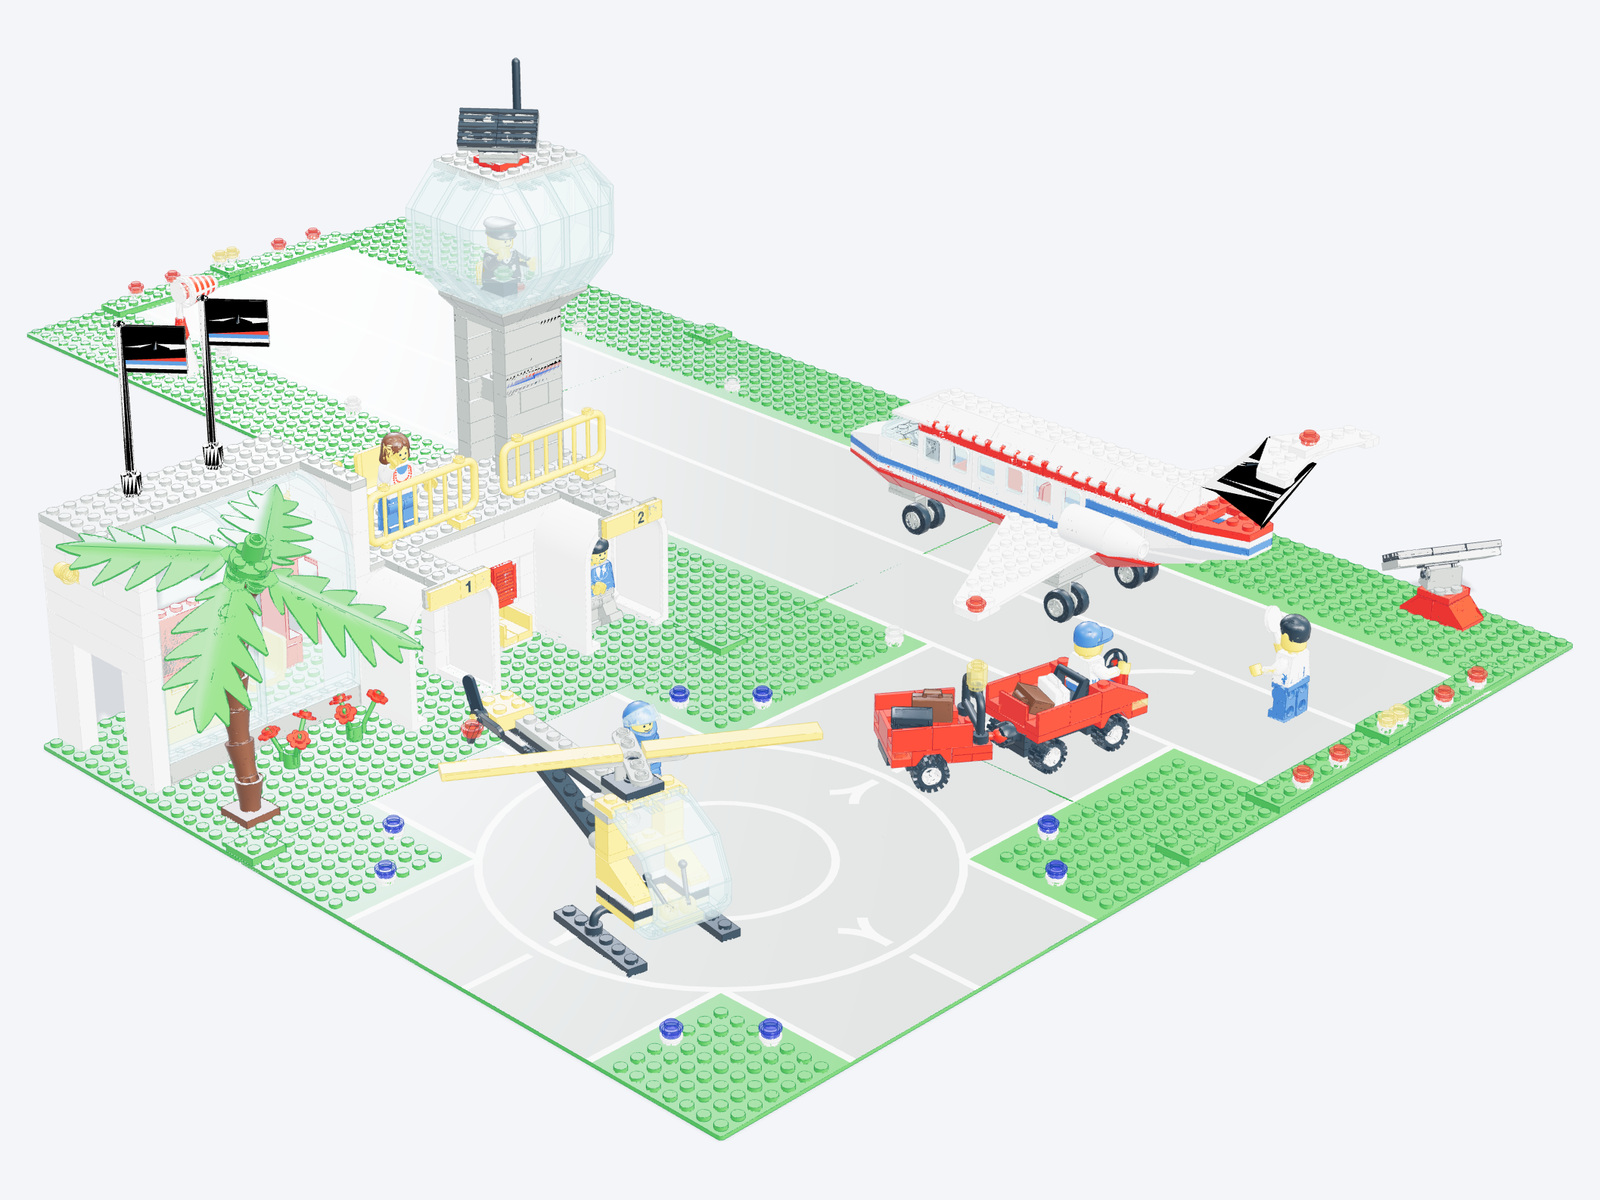
\includegraphics[width=.48\linewidth]{figures/ldraw/print/10159-iso.jpg}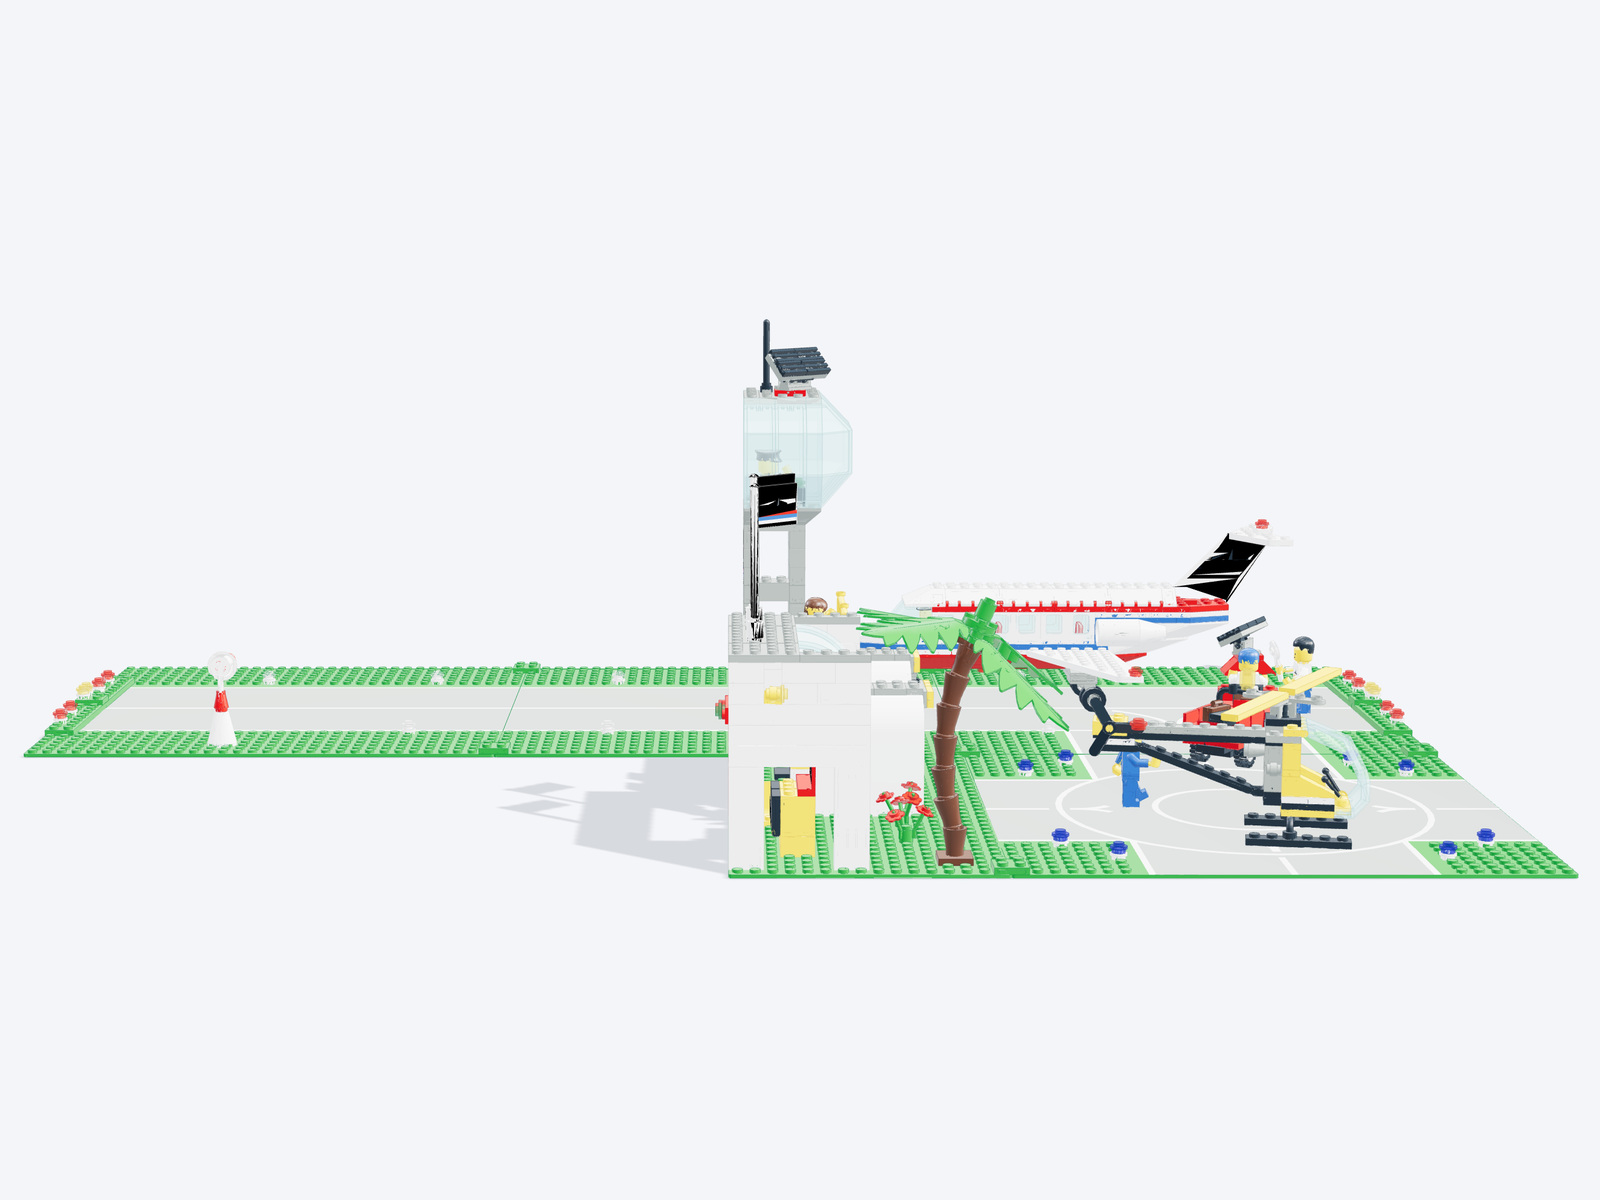
\includegraphics[width=.48\linewidth]{figures/ldraw/print/10159-front.jpg}\\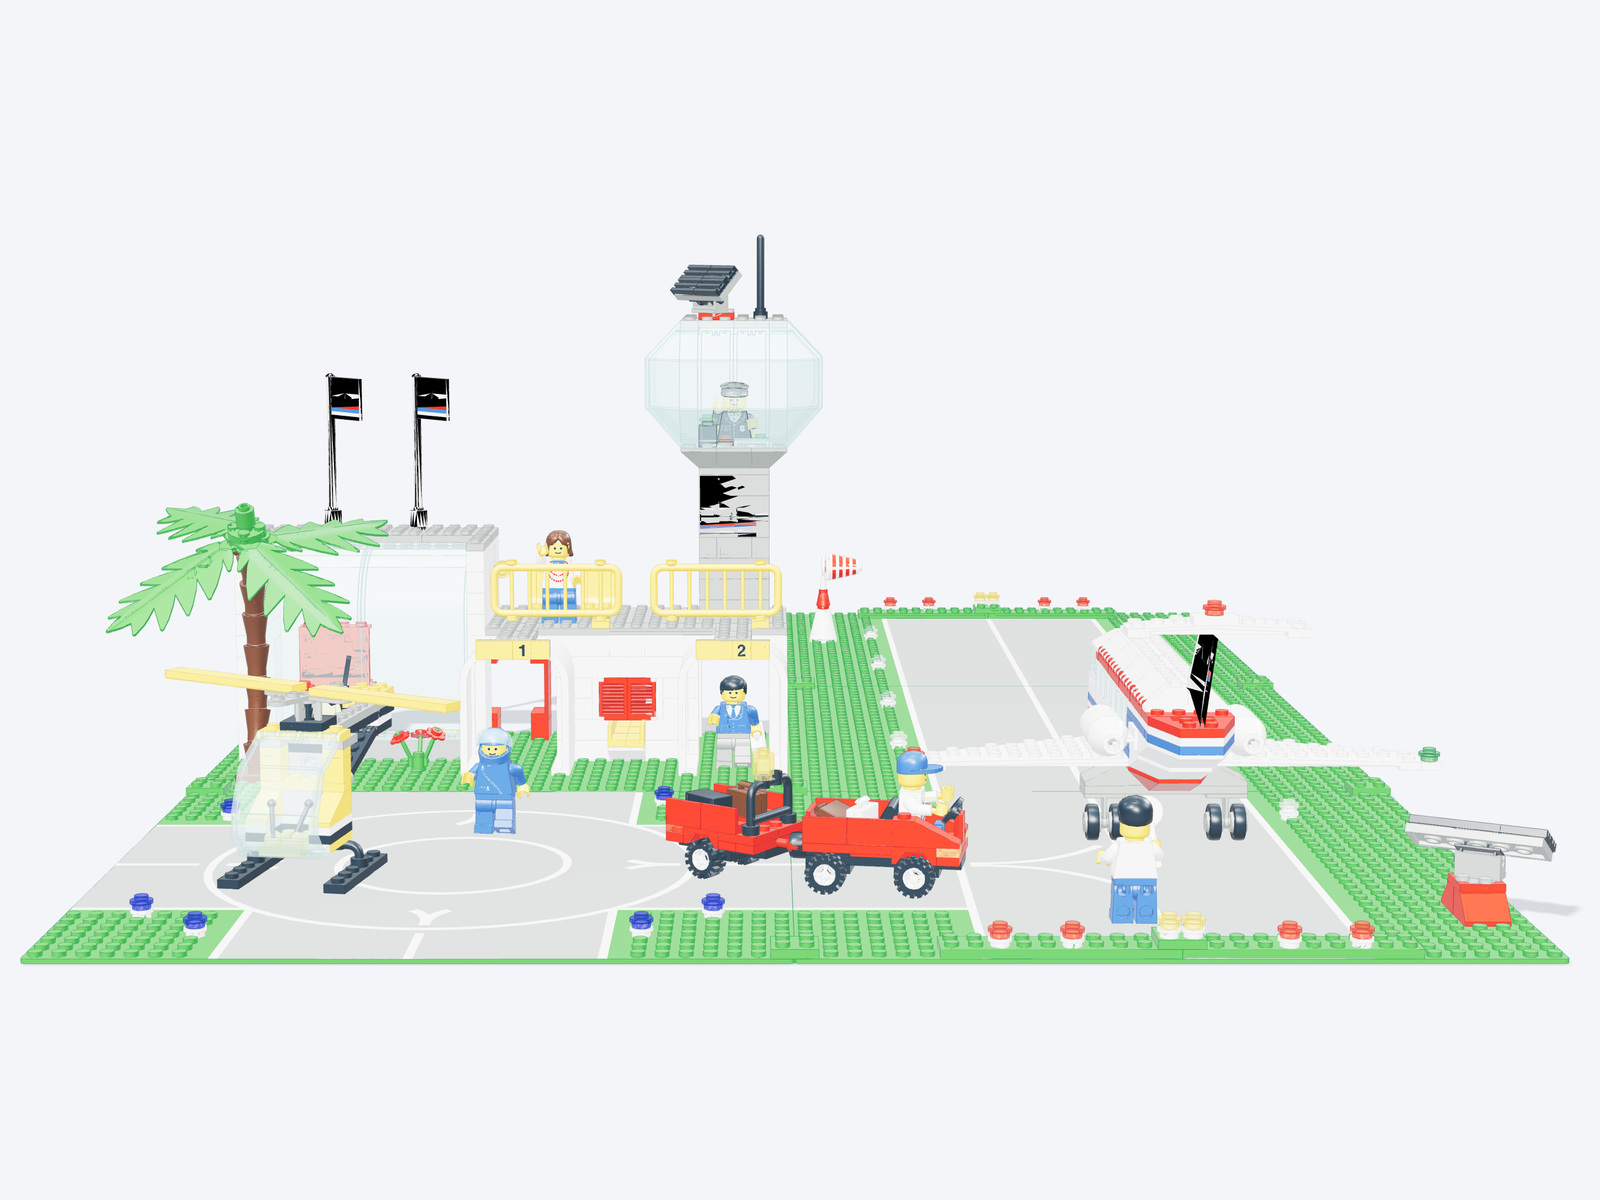
\includegraphics[width=.48\linewidth]{figures/ldraw/print/10159-side.jpg}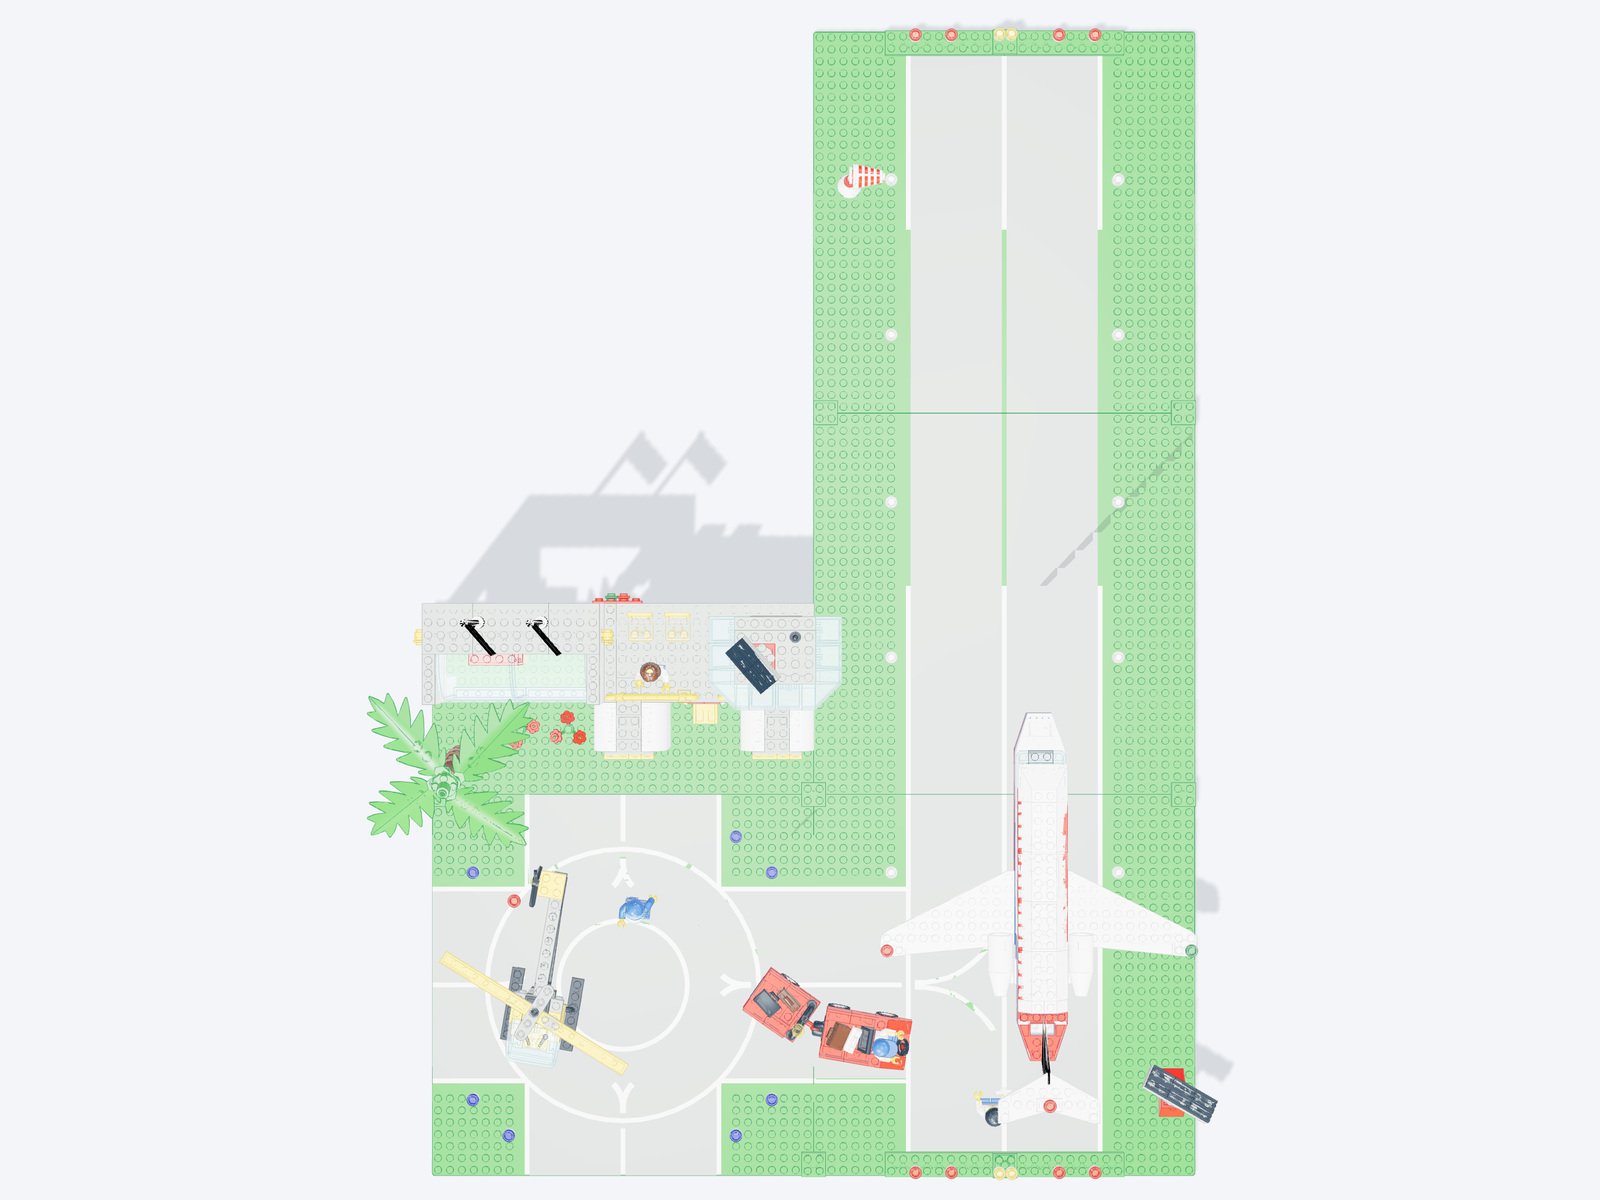
\includegraphics[width=.48\linewidth]{figures/ldraw/print/10159-top.jpg}\end{center}
\paragraph{Attribution.}Zoltan Keri [kzoltan82]. CC BY 2.0.\par\noindent\url{https://library.ldraw.org/omr/sets/660}
\paragraph{Source lock.}\small\texttt{ef0b08af1e69059813e8965d3aa8fdd6}\\\texttt{a4aadbb04a21d92723cc4f9ae26bc1ec}\normalsize
\paragraph{Evidence coverage.}Connector definitions cover 94.93\% of instances. The audit reports 58 recognized-graph components and 26 intersection candidates without a recognized mating pair. 30 instances have no connector definition. These counts do not certify physical defects or gravitational stability.
\paragraph{Instructions.}No author STEP replay or source-order question is provided.
\clearpage\subsection{Numbered visual input and complete question index}
Only relevant numbers are shown. The website can isolate any instance; public visual tasks provide their own numbered images. The following entries give every English prompt, all choice options, compact public evidence and the reference output. Raw repeated connector records and full action fact sets remain in the versioned JSON.
\begin{center}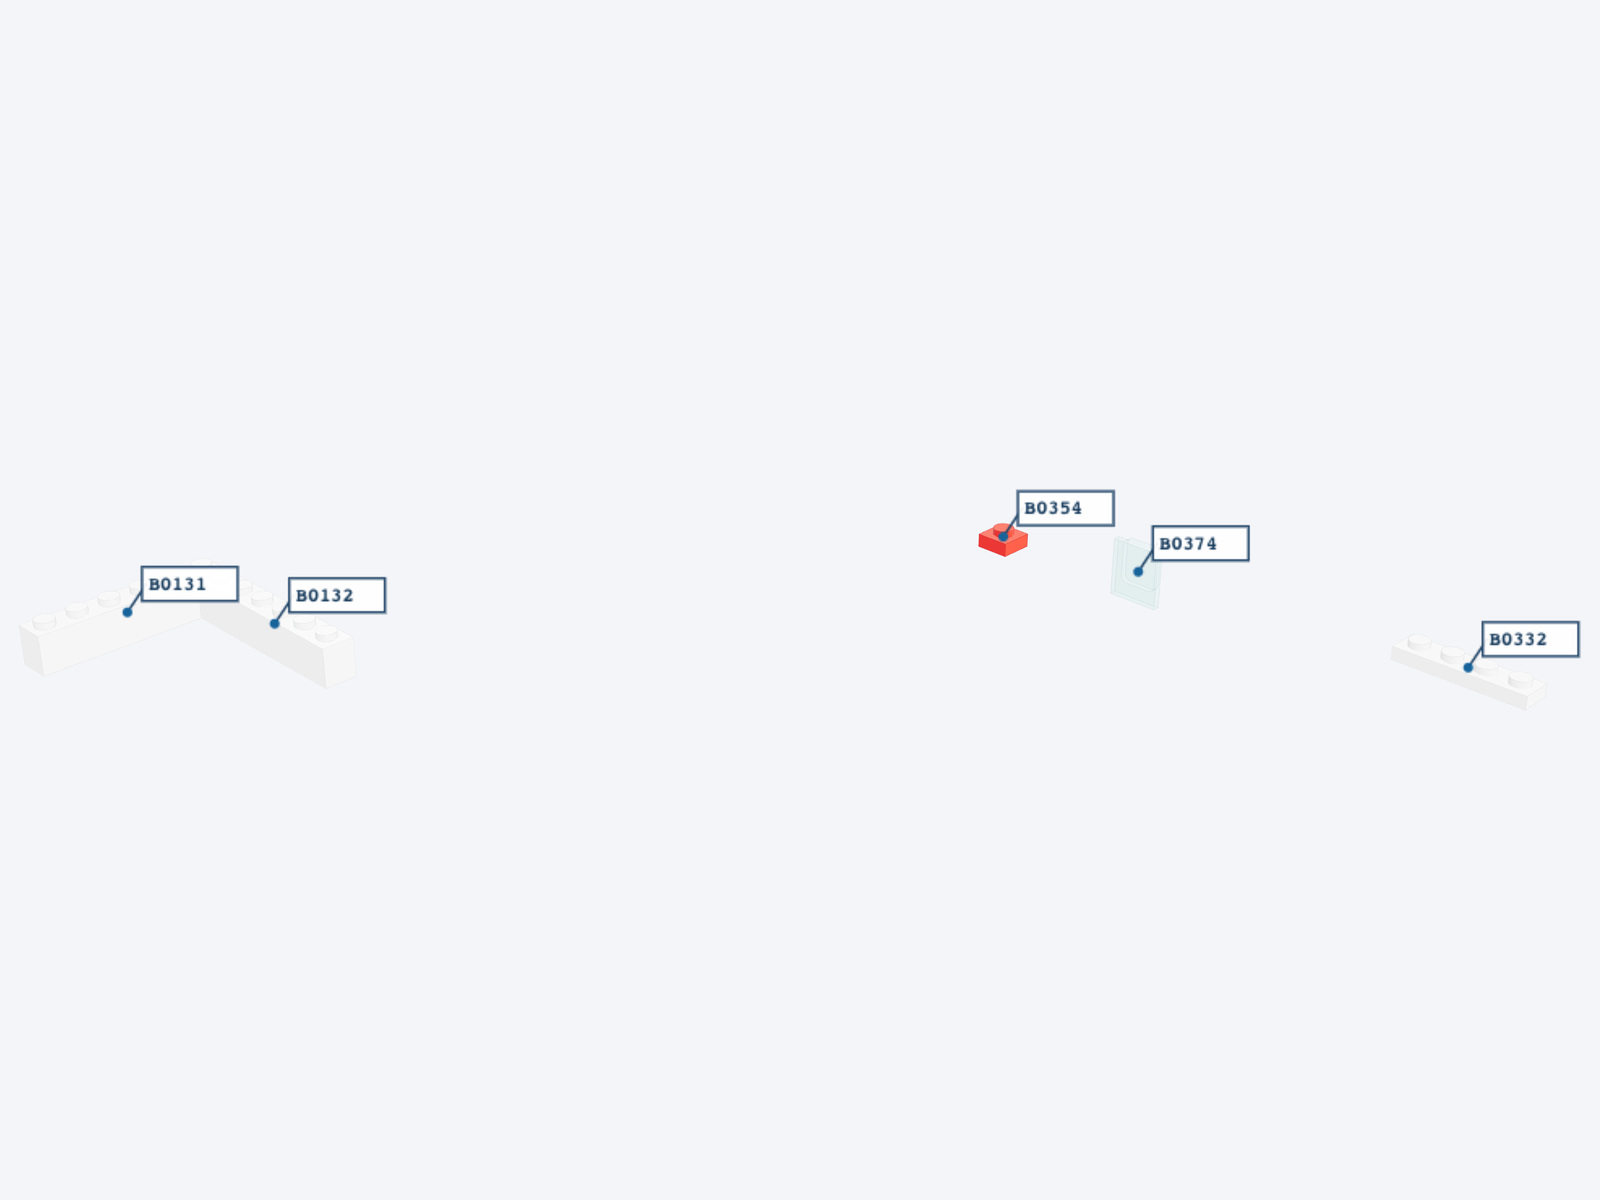
\includegraphics[width=.55\linewidth]{figures/ldraw/print/10159-numbered.jpg}\end{center}
\begin{enumerate}
\item \textbf{color-1}. Identify the original color of B0132; numbered isolation is allowed.\par {\small \textit{Input:} Numbered visual input; source attributes are withheld from the model. \par\textit{Options:} A: Brown; B: Green; C: White; D: Black. \par\textit{Reference output:} C.}
\item \textbf{shape-match-1}. Ignoring color and pose, which numbered instance has the same LDraw part type as B0132?\par {\small \textit{Input:} Numbered visual input; source attributes are withheld from the model. \par\textit{Options:} A: B0332; B: B0374; C: B0354; D: B0131. \par\textit{Reference output:} D.}
\item \textbf{distance-1}. Using the supplied geometry bounding-box centers, which candidate is nearest to B0132?\par {\small \textit{Input:} Centers (mm): B0132 = (124, 53.6, -224); B0234 = (93.534, 213.4228, -211.256); B0138 = (-116, 53.6, -224); B0510 = (255.005523, 23.458353, 71.775633). \par\textit{Options:} A: B0510; B: B0138; C: B0234. \par\textit{Reference output:} C.}
\item \textbf{color-2}. Identify the original color of B0181; numbered isolation is allowed.\par {\small \textit{Input:} Numbered visual input; source attributes are withheld from the model. \par\textit{Options:} A: Blue; B: Trans Light Blue; C: Light Grey; D: Trans Yellow. \par\textit{Reference output:} D.}
\item \textbf{shape-match-2}. Ignoring color and pose, which numbered instance has the same LDraw part type as B0181?\par {\small \textit{Input:} Numbered visual input; source attributes are withheld from the model. \par\textit{Options:} A: B0380; B: B0356; C: B0530; D: B0367. \par\textit{Reference output:} A.}
\item \textbf{distance-2}. Using the supplied geometry bounding-box centers, which candidate is nearest to B0181?\par {\small \textit{Input:} Centers (mm): B0181 = (-4, 82.4, -232); B0297 = (288, 36, -48); B0245 = (-43.4404, 15.721947, -167.7786); B0228 = (96, 200, -224). \par\textit{Options:} A: B0297; B: B0245; C: B0228. \par\textit{Reference output:} B.}
\item \textbf{color-3}. Identify the original color of B0485; numbered isolation is allowed.\par {\small \textit{Input:} Numbered visual input; source attributes are withheld from the model. \par\textit{Options:} A: Yellow; B: Light Grey; C: Trans Red; D: Red. \par\textit{Reference output:} D.}
\item \textbf{shape-match-3}. Ignoring color and pose, which numbered instance has the same LDraw part type as B0485?\par {\small \textit{Input:} Numbered visual input; source attributes are withheld from the model. \par\textit{Options:} A: B0250; B: B0425; C: B0555; D: B0254. \par\textit{Reference output:} B.}
\item \textbf{distance-3}. Using the supplied geometry bounding-box centers, which candidate is nearest to B0485?\par {\small \textit{Input:} Centers (mm): B0485 = (93.602, 14.8, 1.614); B0372 = (290.4, 48, -80); B0560 = (171.7044, 22.058761, 34.162); B0206 = (112, 169.6, -204). \par\textit{Options:} A: B0372; B: B0206; C: B0560. \par\textit{Reference output:} C.}
\item \textbf{interface-1}. Classify the supplied connector record for B0230 and B0231. This does not certify load capacity.\par {\small \textit{Input:} Record: family = axle; connector indices = 1, 1. \par\textit{Options:} A: ball; B: hinge; C: axle; D: fixed. \par\textit{Reference output:} C.}
\item \textbf{interface-2}. Classify the supplied connector record for B0486 and B0454. This does not certify load capacity.\par {\small \textit{Input:} Record: family = ball; connector indices = 4, 0. \par\textit{Options:} A: fixed; B: ball; C: axle; D: hinge. \par\textit{Reference output:} B.}
\item \textbf{interface-3}. Classify the supplied connector record for B0383 and B0387. This does not certify load capacity.\par {\small \textit{Input:} Record: family = fixed; connector indices = 1, 1. \par\textit{Options:} A: ball; B: axle; C: hinge; D: fixed. \par\textit{Reference output:} D.}
\item \textbf{interface-4}. Classify the supplied connector record for B0539 and B0545. This does not certify load capacity.\par {\small \textit{Input:} Record: family = hinge; connector indices = 3, 1. \par\textit{Options:} A: ball; B: fixed; C: hinge; D: axle. \par\textit{Reference output:} C.}
\item \textbf{interface-5}. Classify the supplied connector record for B0089 and B0122. This does not certify load capacity.\par {\small \textit{Input:} Record: family = stud; connector indices = 14, 4. \par\textit{Options:} A: stud; B: fixed; C: axle; D: ball; E: hinge. \par\textit{Reference output:} A.}
\item \textbf{neighbors-1}. Select every candidate directly adjacent to B0079 in the supplied connector graph.\par {\small \textit{Input:} Unique undirected pairs: B0078 / B0079; B0079 / B0080; B0079 / B0081. \par\textit{Options:} A: B0080; B: B0081; C: B0078; D: B0283; E: B0525. \par\textit{Reference output:} A, B, C.}
\item \textbf{graph-removal-1}. Delete B0079 and its incident edges from this local graph. How many connected components remain? Do not infer physical extractability.\par {\small \textit{Input:} Nodes: B0079, B0080, B0081, B0078, B0283, B0525. Unique undirected pairs: B0078 / B0079; B0079 / B0080; B0079 / B0081. \par\textit{Options:} A: 5; B: 7; C: 6; D: 4. \par\textit{Reference output:} A.}
\item \textbf{neighbors-2}. Select every candidate directly adjacent to B0353 in the supplied connector graph.\par {\small \textit{Input:} Unique undirected pairs: B0336 / B0353; B0353 / B0375. \par\textit{Options:} A: B0336; B: B0112; C: B0375; D: B0186. \par\textit{Reference output:} A, C.}
\item \textbf{graph-removal-2}. Delete B0353 and its incident edges from this local graph. How many connected components remain? Do not infer physical extractability.\par {\small \textit{Input:} Nodes: B0353, B0336, B0375, B0112, B0186. Unique undirected pairs: B0336 / B0353; B0353 / B0375. \par\textit{Options:} A: 4; B: 6; C: 3; D: 5. \par\textit{Reference output:} A.}
\item \textbf{neighbors-3}. Select every candidate directly adjacent to B0328 in the supplied connector graph.\par {\small \textit{Input:} Unique undirected pairs: B0325 / B0328; B0328 / B0351. \par\textit{Options:} A: B0560; B: B0351; C: B0325; D: B0185. \par\textit{Reference output:} B, C.}
\item \textbf{graph-removal-3}. Delete B0328 and its incident edges from this local graph. How many connected components remain? Do not infer physical extractability.\par {\small \textit{Input:} Nodes: B0328, B0325, B0351, B0185, B0560. Unique undirected pairs: B0325 / B0328; B0328 / B0351. \par\textit{Options:} A: 3; B: 6; C: 4; D: 5. \par\textit{Reference output:} C.}
\item \textbf{coverage-1}. Which numbered instance lacks a connector definition in the coverage record, so this audit cannot establish that it is floating?\par {\small \textit{Input:} Definition coverage: B0238 = unsupported; B0132 = supported; B0181 = supported; B0485 = supported. \par\textit{Options:} A: B0485; B: B0181; C: B0132; D: B0238. \par\textit{Reference output:} D.}
\item \textbf{evidence-limit-1}. Only source geometry, connector matching and mesh intersection audits are available. Without mass, friction, material or dynamic tests, is gravitational stability established?\par {\small \textit{Input:} Available evidence: Original CAD; Connector inference; Inset-mesh intersection candidates. \par\textit{Options:} A: Established; B: Not established by this evidence. \par\textit{Reference output:} B.}
\item \textbf{restore-instance-1}. The display copy hides B0132. Restore only that numbered instance, preserving all other instances and source poses.\par {\small \textit{Input:} Target: B0132. Action budget: 1. All other instances initially remain visible. \par\textit{Reference output:} restore-B0132.}
\item \textbf{restore-instance-2}. The display copy hides B0181. Restore only that numbered instance, preserving all other instances and source poses.\par {\small \textit{Input:} Target: B0181. Action budget: 1. All other instances initially remain visible. \par\textit{Reference output:} restore-B0181.}
\item \textbf{restore-instance-3}. The display copy hides B0485. Restore only that numbered instance, preserving all other instances and source poses.\par {\small \textit{Input:} Target: B0485. Action budget: 1. All other instances initially remain visible. \par\textit{Reference output:} restore-B0485.}
\end{enumerate}
\clearpage
\section{10001: Metroliner}
848 source instances; 34 tasks; D3 scale band.

\par\noindent Perspective, front, side and top views follow in reading order. Original source transforms are preserved.
\begin{center}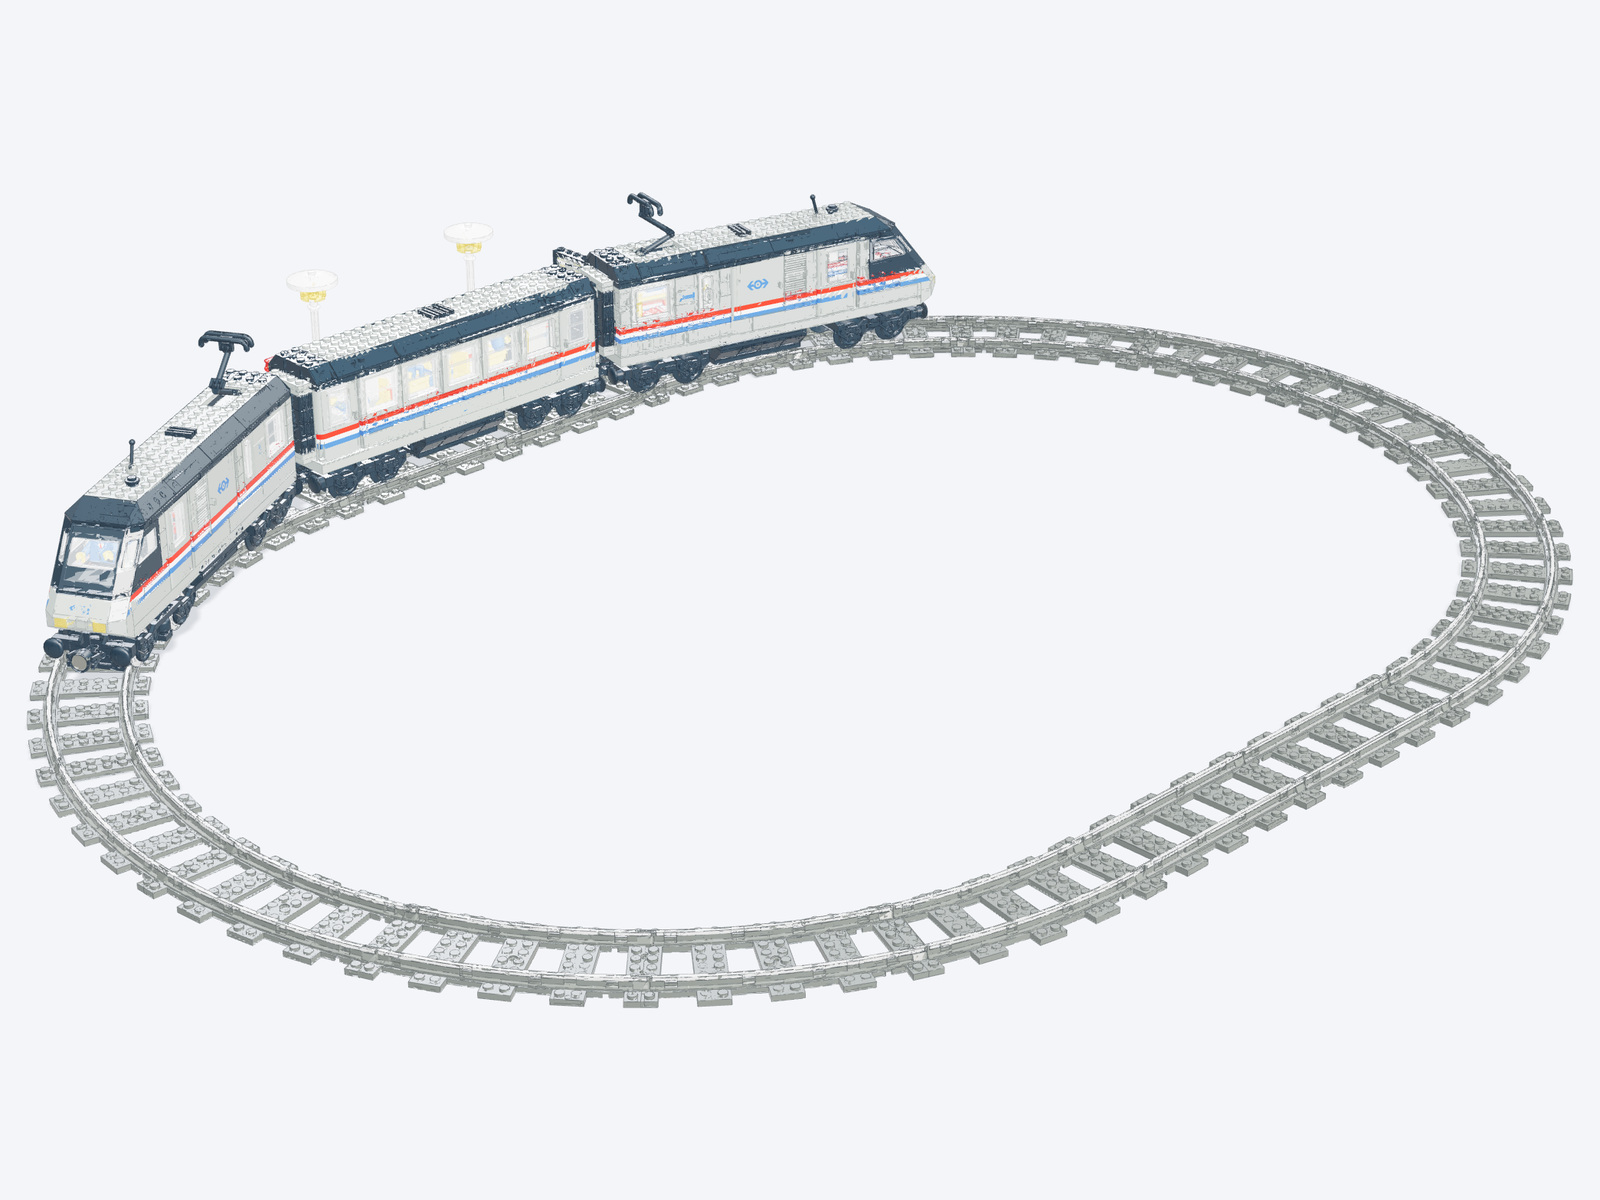
\includegraphics[width=.48\linewidth]{figures/ldraw/print/10001-iso.jpg}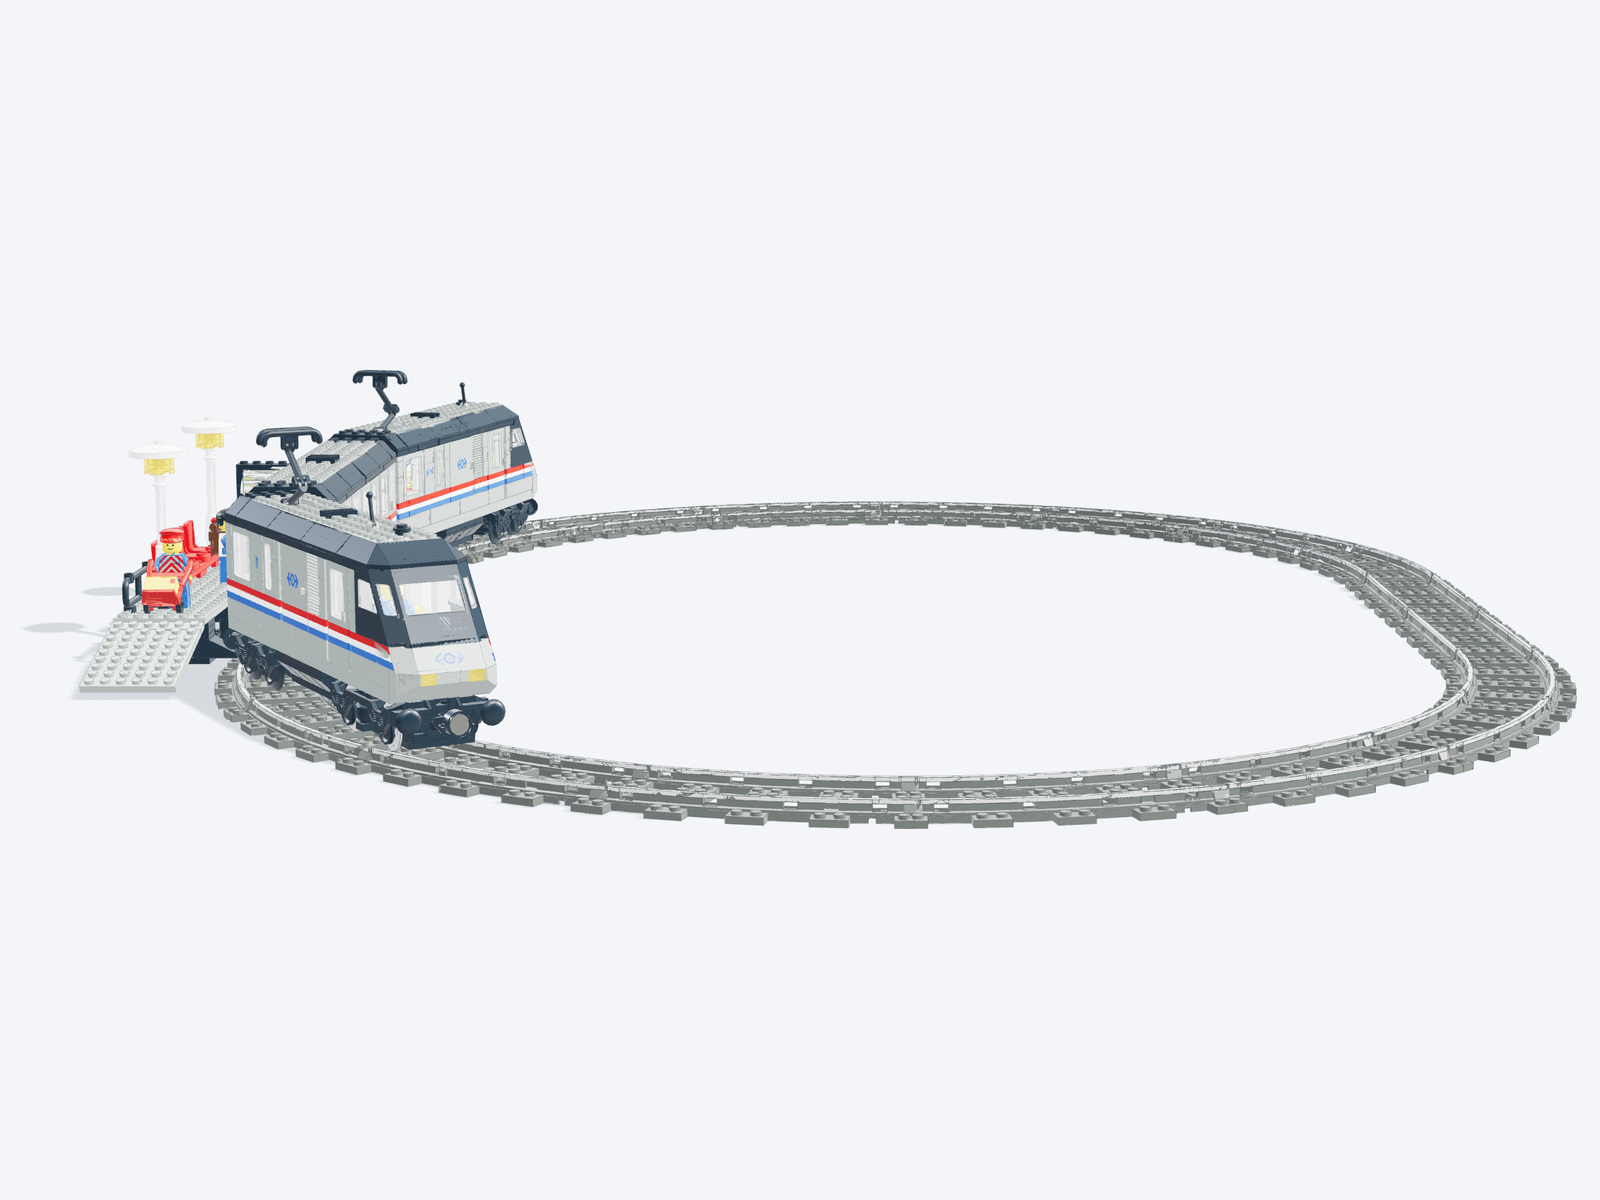
\includegraphics[width=.48\linewidth]{figures/ldraw/print/10001-front.jpg}\\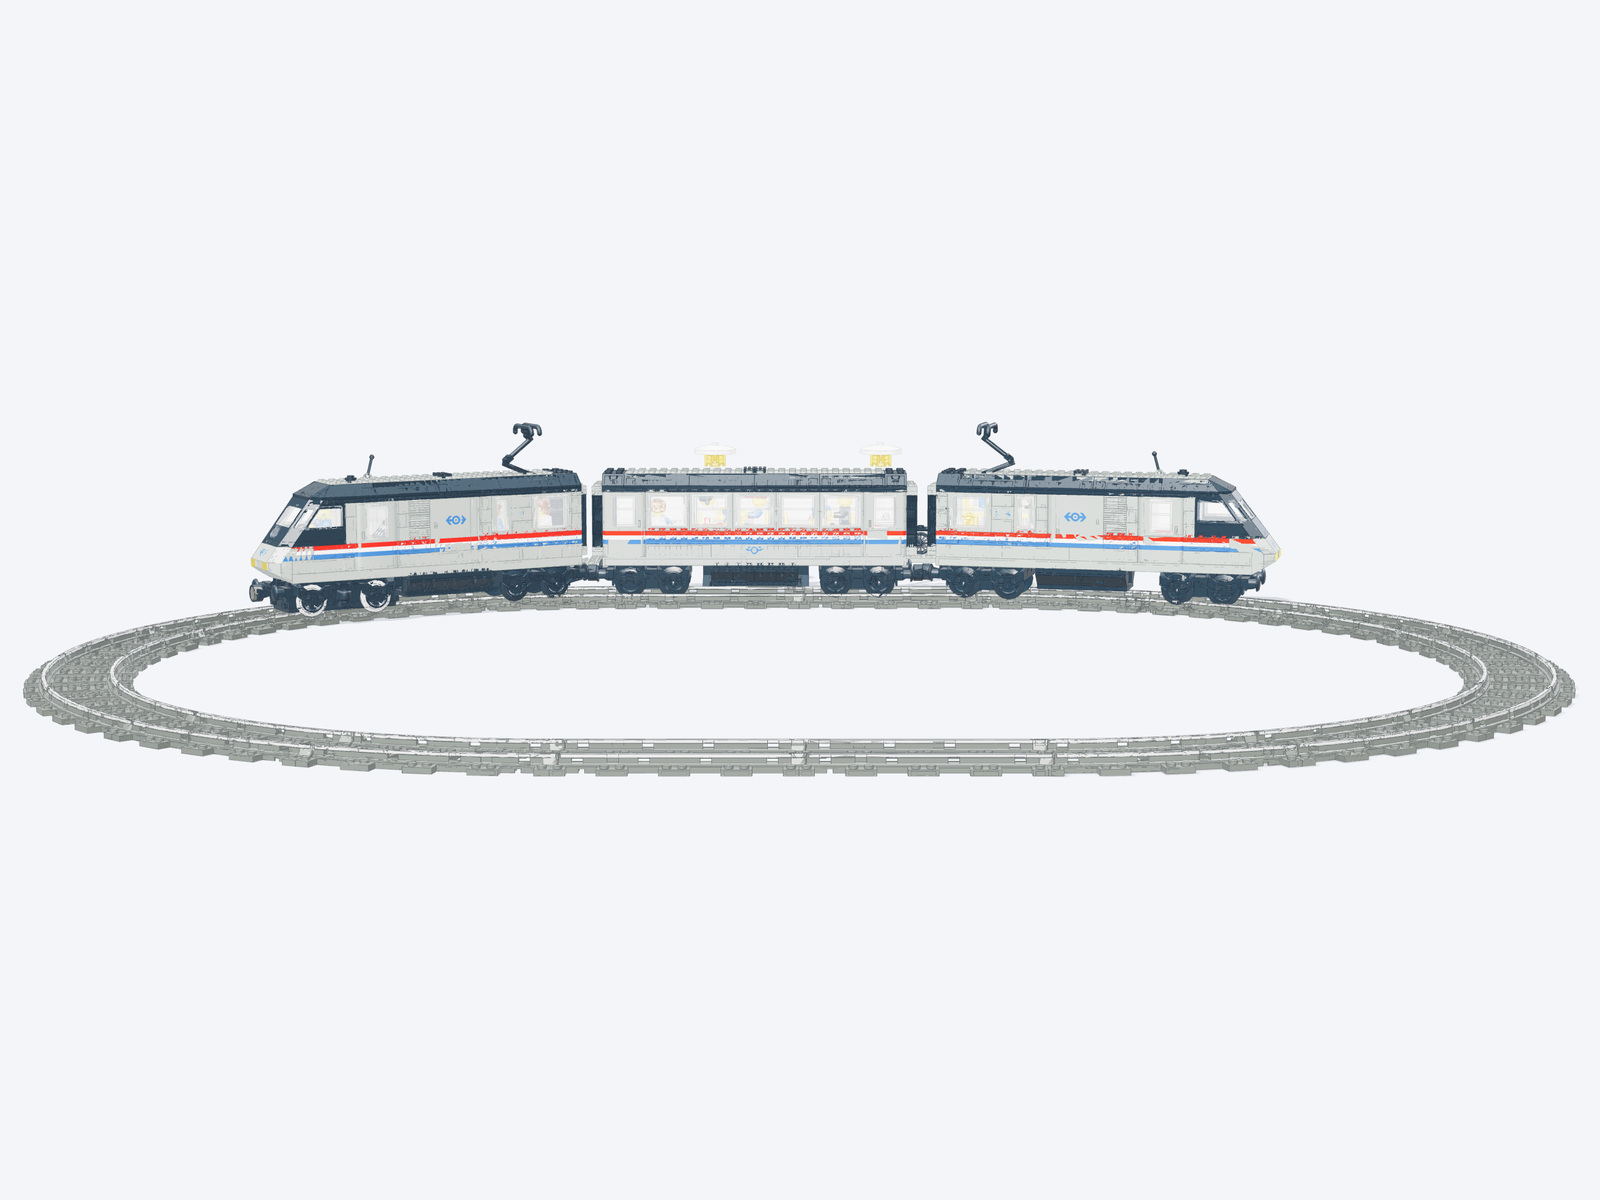
\includegraphics[width=.48\linewidth]{figures/ldraw/print/10001-side.jpg}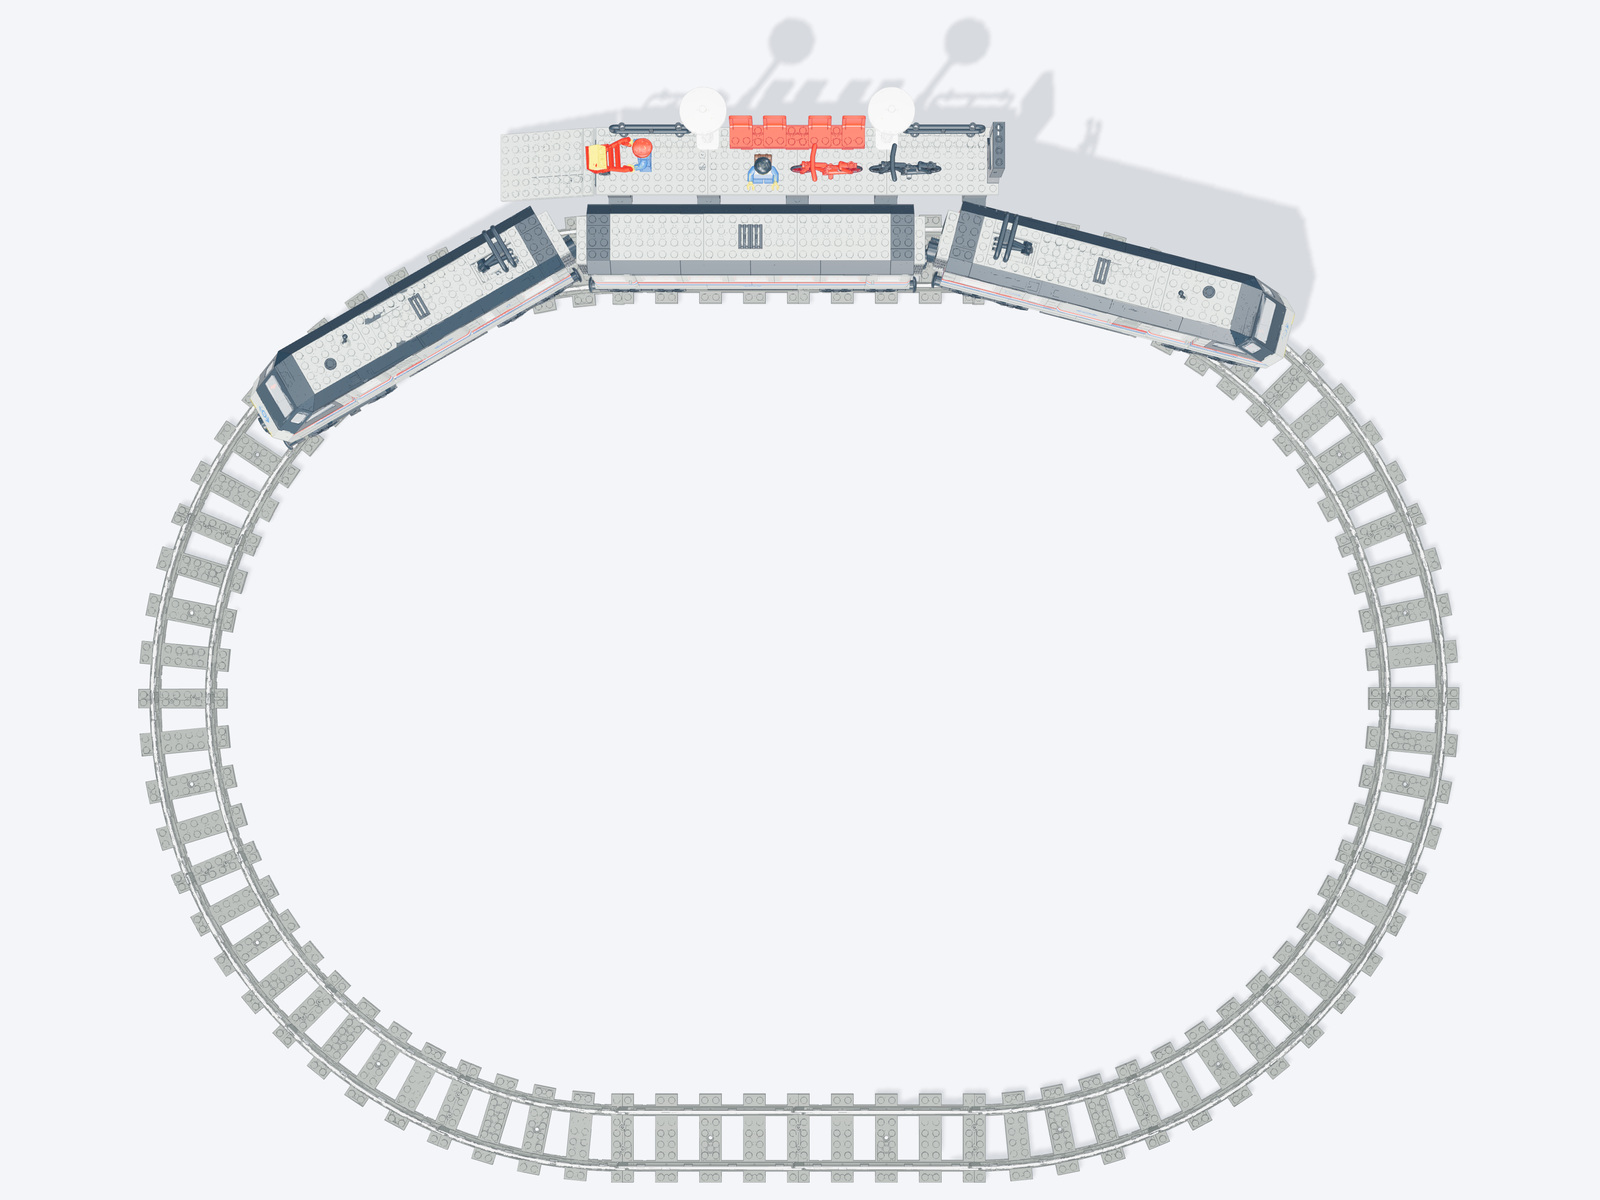
\includegraphics[width=.48\linewidth]{figures/ldraw/print/10001-top.jpg}\end{center}
\paragraph{Attribution.}Zoltan Keri [kzoltan82]. CC BY 2.0.\par\noindent\url{https://library.ldraw.org/omr/sets/657}
\paragraph{Source lock.}\small\texttt{684a8032488dc2c5cb72a9ef32befb13}\\\texttt{99914eb32423e5b0cd91b6acfd3ab0e3}\normalsize
\paragraph{Evidence coverage.}Connector definitions cover 94.34\% of instances. The audit reports 90 recognized-graph components and 75 intersection candidates without a recognized mating pair. 48 instances have no connector definition. These counts do not certify physical defects or gravitational stability.
\paragraph{Instructions.}26 expanded author steps.
\clearpage\subsection{Numbered visual input and complete question index}
Only relevant numbers are shown. The website can isolate any instance; public visual tasks provide their own numbered images. The following entries give every English prompt, all choice options, compact public evidence and the reference output. Raw repeated connector records and full action fact sets remain in the versioned JSON.
\begin{center}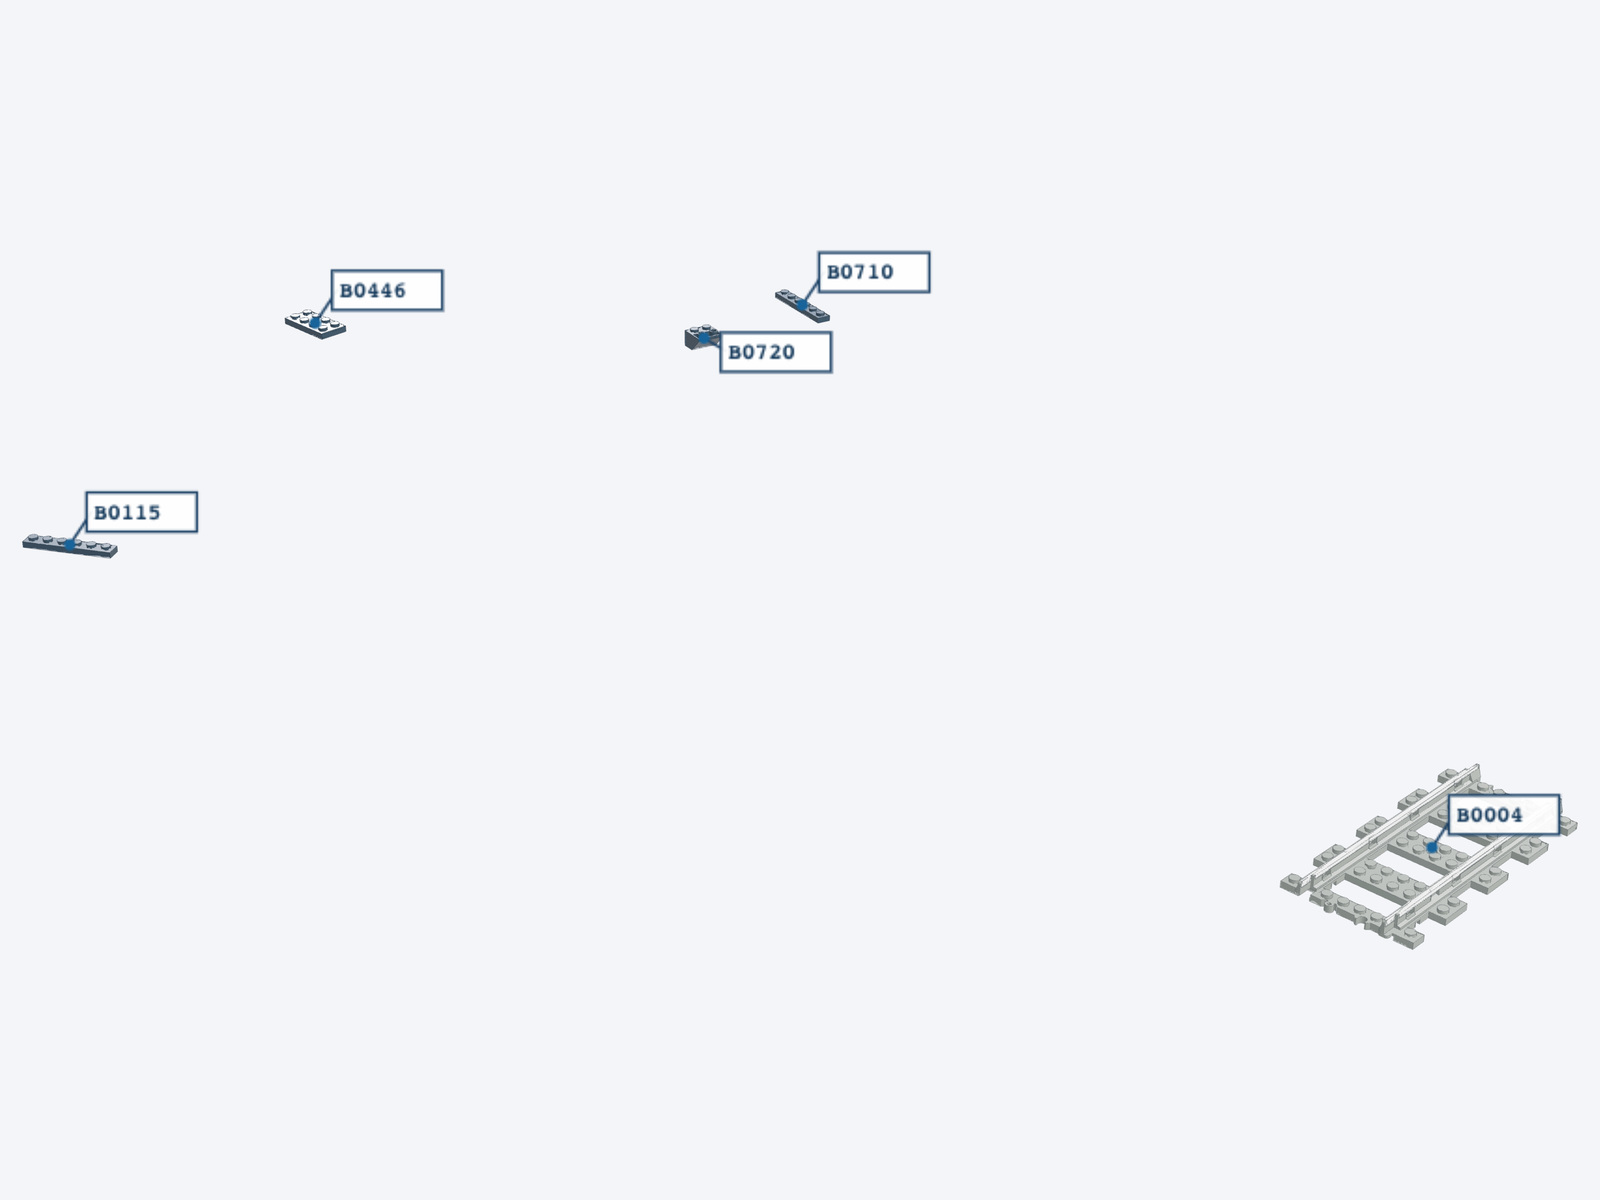
\includegraphics[width=.55\linewidth]{figures/ldraw/print/10001-numbered.jpg}\end{center}
\begin{enumerate}
\item \textbf{color-1}. Identify the original color of B0115; numbered isolation is allowed.\par {\small \textit{Input:} Numbered visual input; source attributes are withheld from the model. \par\textit{Options:} A: Black; B: Trans Clear; C: Trans Yellow; D: White. \par\textit{Reference output:} A.}
\item \textbf{shape-match-1}. Ignoring color and pose, which numbered instance has the same LDraw part type as B0115?\par {\small \textit{Input:} Numbered visual input; source attributes are withheld from the model. \par\textit{Options:} A: B0710; B: B0720; C: B0004; D: B0446. \par\textit{Reference output:} A.}
\item \textbf{distance-1}. Using the supplied geometry bounding-box centers, which candidate is nearest to B0115?\par {\small \textit{Input:} Centers (mm): B0115 = (-74.436799, 20.8, 3.551199); B0720 = (343.856, 20.8, 30.516); B0050 = (-39.756, 13.2228, -92); B0272 = (-109.031199, 68.8, 0.431199). \par\textit{Options:} A: B0050; B: B0272; C: B0720. \par\textit{Reference output:} B.}
\item \textbf{color-2}. Identify the original color of B0159; numbered isolation is allowed.\par {\small \textit{Input:} Numbered visual input; source attributes are withheld from the model. \par\textit{Options:} A: Black; B: White; C: Brown; D: Light Grey. \par\textit{Reference output:} D.}
\item \textbf{shape-match-2}. Ignoring color and pose, which numbered instance has the same LDraw part type as B0159?\par {\small \textit{Input:} Numbered visual input; source attributes are withheld from the model. \par\textit{Options:} A: B0165; B: B0163; C: B0192; D: B0794. \par\textit{Reference output:} B.}
\item \textbf{distance-2}. Using the supplied geometry bounding-box centers, which candidate is nearest to B0159?\par {\small \textit{Input:} Centers (mm): B0159 = (-157.527199, 40, 28.431199); B0350 = (-140.599199, 88, 41.751199); B0637 = (370.82, 59.2, 41.768); B0018 = (-178.751951, 1.6, 570.031873). \par\textit{Options:} A: B0350; B: B0637; C: B0018. \par\textit{Reference output:} A.}
\item \textbf{color-3}. Identify the original color of B0739; numbered isolation is allowed.\par {\small \textit{Input:} Numbered visual input; source attributes are withheld from the model. \par\textit{Options:} A: Black; B: White; C: Light Grey; D: Trans Yellow. \par\textit{Reference output:} A.}
\item \textbf{shape-match-3}. Ignoring color and pose, which numbered instance has the same LDraw part type as B0739?\par {\small \textit{Input:} Numbered visual input; source attributes are withheld from the model. \par\textit{Options:} A: B0712; B: B0776; C: B0023; D: B0546. \par\textit{Reference output:} A.}
\item \textbf{distance-3}. Using the supplied geometry bounding-box centers, which candidate is nearest to B0739?\par {\small \textit{Input:} Centers (mm): B0739 = (275.744, 23.2, -21.2716); B0816 = (316.144, 59.2, -10.808); B0474 = (64, 40, -20); B0770 = (274.873286, 99.670801, -5.26347). \par\textit{Options:} A: B0770; B: B0474; C: B0816. \par\textit{Reference output:} C.}
\item \textbf{color-4}. Identify the original color of B0826; numbered isolation is allowed.\par {\small \textit{Input:} Numbered visual input; source attributes are withheld from the model. \par\textit{Options:} A: Trans Clear; B: Black; C: White; D: Brown. \par\textit{Reference output:} B.}
\item \textbf{shape-match-4}. Ignoring color and pose, which numbered instance has the same LDraw part type as B0826?\par {\small \textit{Input:} Numbered visual input; source attributes are withheld from the model. \par\textit{Options:} A: B0581; B: B0137; C: B0121; D: B0079. \par\textit{Reference output:} C.}
\item \textbf{distance-4}. Using the supplied geometry bounding-box centers, which candidate is nearest to B0826?\par {\small \textit{Input:} Centers (mm): B0826 = (230.90065, 19.05, -16.2808); B0373 = (208, 56, 0); B0666 = (369.2836, 78.4, -1.4436); B0599 = (254.82, 40, 11.724). \par\textit{Options:} A: B0599; B: B0373; C: B0666. \par\textit{Reference output:} A.}
\item \textbf{interface-1}. Classify the supplied connector record for B0476 and B0477. This does not certify load capacity.\par {\small \textit{Input:} Record: family = axle; connector indices = 0, 0. \par\textit{Options:} A: fixed; B: hinge; C: axle; D: ball. \par\textit{Reference output:} C.}
\item \textbf{interface-2}. Classify the supplied connector record for B0101 and B0103. This does not certify load capacity.\par {\small \textit{Input:} Record: family = fixed; connector indices = 3, 1. \par\textit{Options:} A: hinge; B: axle; C: ball; D: fixed. \par\textit{Reference output:} D.}
\item \textbf{interface-3}. Classify the supplied connector record for B0840 and B0845. This does not certify load capacity.\par {\small \textit{Input:} Record: family = hinge; connector indices = 0, 6. \par\textit{Options:} A: ball; B: hinge; C: axle; D: fixed. \par\textit{Reference output:} B.}
\item \textbf{interface-4}. Classify the supplied connector record for B0592 and B0787. This does not certify load capacity.\par {\small \textit{Input:} Record: family = stud; connector indices = 225, 7. \par\textit{Options:} A: hinge; B: stud; C: axle; D: ball; E: fixed. \par\textit{Reference output:} B.}
\item \textbf{neighbors-1}. Select every candidate directly adjacent to B0058 in the supplied connector graph.\par {\small \textit{Input:} Unique undirected pairs: B0052 / B0058; B0053 / B0058; B0058 / B0076. \par\textit{Options:} A: B0653; B: B0076; C: B0484; D: B0052; E: B0053. \par\textit{Reference output:} B, D, E.}
\item \textbf{graph-removal-1}. Delete B0058 and its incident edges from this local graph. How many connected components remain? Do not infer physical extractability.\par {\small \textit{Input:} Nodes: B0058, B0076, B0052, B0053, B0653, B0484. Unique undirected pairs: B0052 / B0058; B0053 / B0058; B0058 / B0076. \par\textit{Options:} A: 6; B: 5; C: 4; D: 7. \par\textit{Reference output:} B.}
\item \textbf{neighbors-2}. Select every candidate directly adjacent to B0734 in the supplied connector graph.\par {\small \textit{Input:} Unique undirected pairs: B0729 / B0734; B0731 / B0734; B0733 / B0734. \par\textit{Options:} A: B0731; B: B0733; C: B0729; D: B0233; E: B0013. \par\textit{Reference output:} A, B, C.}
\item \textbf{graph-removal-2}. Delete B0734 and its incident edges from this local graph. How many connected components remain? Do not infer physical extractability.\par {\small \textit{Input:} Nodes: B0734, B0729, B0731, B0733, B0233, B0013. Unique undirected pairs: B0729 / B0734; B0731 / B0734; B0733 / B0734. \par\textit{Options:} A: 7; B: 6; C: 5; D: 4. \par\textit{Reference output:} C.}
\item \textbf{neighbors-3}. Select every candidate directly adjacent to B0828 in the supplied connector graph.\par {\small \textit{Input:} Unique undirected pairs: B0828 / B0833; B0828 / B0834; B0828 / B0836. \par\textit{Options:} A: B0677; B: B0549; C: B0836; D: B0833; E: B0834. \par\textit{Reference output:} C, D, E.}
\item \textbf{graph-removal-3}. Delete B0828 and its incident edges from this local graph. How many connected components remain? Do not infer physical extractability.\par {\small \textit{Input:} Nodes: B0828, B0833, B0834, B0836, B0677, B0549. Unique undirected pairs: B0828 / B0833; B0828 / B0834; B0828 / B0836. \par\textit{Options:} A: 6; B: 4; C: 5; D: 7. \par\textit{Reference output:} C.}
\item \textbf{neighbors-4}. Select every candidate directly adjacent to B0447 in the supplied connector graph.\par {\small \textit{Input:} Unique undirected pairs: B0439 / B0447; B0440 / B0447; B0442 / B0447; B0444 / B0447; B0445 / B0447. \par\textit{Options:} A: B0593; B: B0440; C: B0439; D: B0012; E: B0445; F: B0442; G: B0444. \par\textit{Reference output:} B, C, E, F, G.}
\item \textbf{graph-removal-4}. Delete B0447 and its incident edges from this local graph. How many connected components remain? Do not infer physical extractability.\par {\small \textit{Input:} Nodes: B0447, B0439, B0442, B0440, B0445, B0444, B0012, B0593. Unique undirected pairs: B0439 / B0447; B0440 / B0447; B0442 / B0447; B0444 / B0447; B0445 / B0447. \par\textit{Options:} A: 7; B: 8; C: 9; D: 6. \par\textit{Reference output:} A.}
\item \textbf{coverage-1}. Which numbered instance lacks a connector definition in the coverage record, so this audit cannot establish that it is floating?\par {\small \textit{Input:} Definition coverage: B0092 = unsupported; B0115 = supported; B0159 = supported; B0739 = supported. \par\textit{Options:} A: B0092; B: B0159; C: B0115; D: B0739. \par\textit{Reference output:} A.}
\item \textbf{evidence-limit-1}. Only source geometry, connector matching and mesh intersection audits are available. Without mass, friction, material or dynamic tests, is gravitational stability established?\par {\small \textit{Input:} Available evidence: Original CAD; Connector inference; Inset-mesh intersection candidates. \par\textit{Options:} A: Established; B: Not established by this evidence. \par\textit{Reference output:} B.}
\item \textbf{source-step-1}. At which expanded author step does B0037 first appear in the supplied source-step table? Source order is not a collision-free assembly proof.\par {\small \textit{Input:} Expanded author records: step 1: B0001; step 4: B0037. \par\textit{Options:} A: 5; B: 3; C: 6; D: 4. \par\textit{Reference output:} D.}
\item \textbf{source-step-2}. At which expanded author step does B0079 first appear in the supplied source-step table? Source order is not a collision-free assembly proof.\par {\small \textit{Input:} Expanded author records: step 1: B0001; step 7: B0079. \par\textit{Options:} A: 6; B: 7; C: 8; D: 9. \par\textit{Reference output:} B.}
\item \textbf{source-step-3}. At which expanded author step does B0052 first appear in the supplied source-step table? Source order is not a collision-free assembly proof.\par {\small \textit{Input:} Expanded author records: step 1: B0001; step 5: B0052. \par\textit{Options:} A: 5; B: 4; C: 7; D: 6. \par\textit{Reference output:} A.}
\item \textbf{source-step-4}. At which expanded author step does B0104 first appear in the supplied source-step table? Source order is not a collision-free assembly proof.\par {\small \textit{Input:} Expanded author records: step 1: B0001; step 9: B0104. \par\textit{Options:} A: 10; B: 8; C: 9; D: 11. \par\textit{Reference output:} C.}
\item \textbf{source-sequence-1}. Reveal the supplied source-step window in author order. Actions change visibility only, without simulating insertion trajectories.\par {\small \textit{Input:} Source window: step-1: B0001, B0002, B0003, B0004, B0005, B0006, B0007, B0008, B0009, B0010, B0011, B0012, B0013, B0014, B0015, B0016, B0017, B0018, B0019, B0020; step-2: B0021, B0022, B0023, B0024, B0025; step-3: B0026, B0027, B0028, B0029, B0030, B0031, B0032, B0033, B0034, B0035, B0036; step-4: B0037, B0038, B0039, B0040, B0041, B0042, B0043, B0044, B0045, B0046, B0047, B0048, B0049, B0050, B0051; step-5: B0052, B0053, B0054, B0055, B0056, B0057; step-6: B0058, B0059, B0060, B0061, B0062, B0063, B0064, B0065, B0066, B0067, B0068, B0069, B0070, B0071, B0072, B0073, B0074, B0075, B0076, B0077, B0078. Action budget: 6. \par\textit{Reference output:} step-1, step-2, step-3, step-4, step-5, step-6.}
\item \textbf{restore-instance-1}. The display copy hides B0115. Restore only that numbered instance, preserving all other instances and source poses.\par {\small \textit{Input:} Target: B0115. Action budget: 1. All other instances initially remain visible. \par\textit{Reference output:} restore-B0115.}
\item \textbf{restore-instance-2}. The display copy hides B0159. Restore only that numbered instance, preserving all other instances and source poses.\par {\small \textit{Input:} Target: B0159. Action budget: 1. All other instances initially remain visible. \par\textit{Reference output:} restore-B0159.}
\item \textbf{restore-instance-3}. The display copy hides B0739. Restore only that numbered instance, preserving all other instances and source poses.\par {\small \textit{Input:} Target: B0739. Action budget: 1. All other instances initially remain visible. \par\textit{Reference output:} restore-B0739.}
\end{enumerate}
\clearpage
\section{10269: Harley-Davidson Fat Boy}
1029 source instances; 34 tasks; D4 scale band.

\par\noindent Perspective, front, side and top views follow in reading order. Original source transforms are preserved.
\begin{center}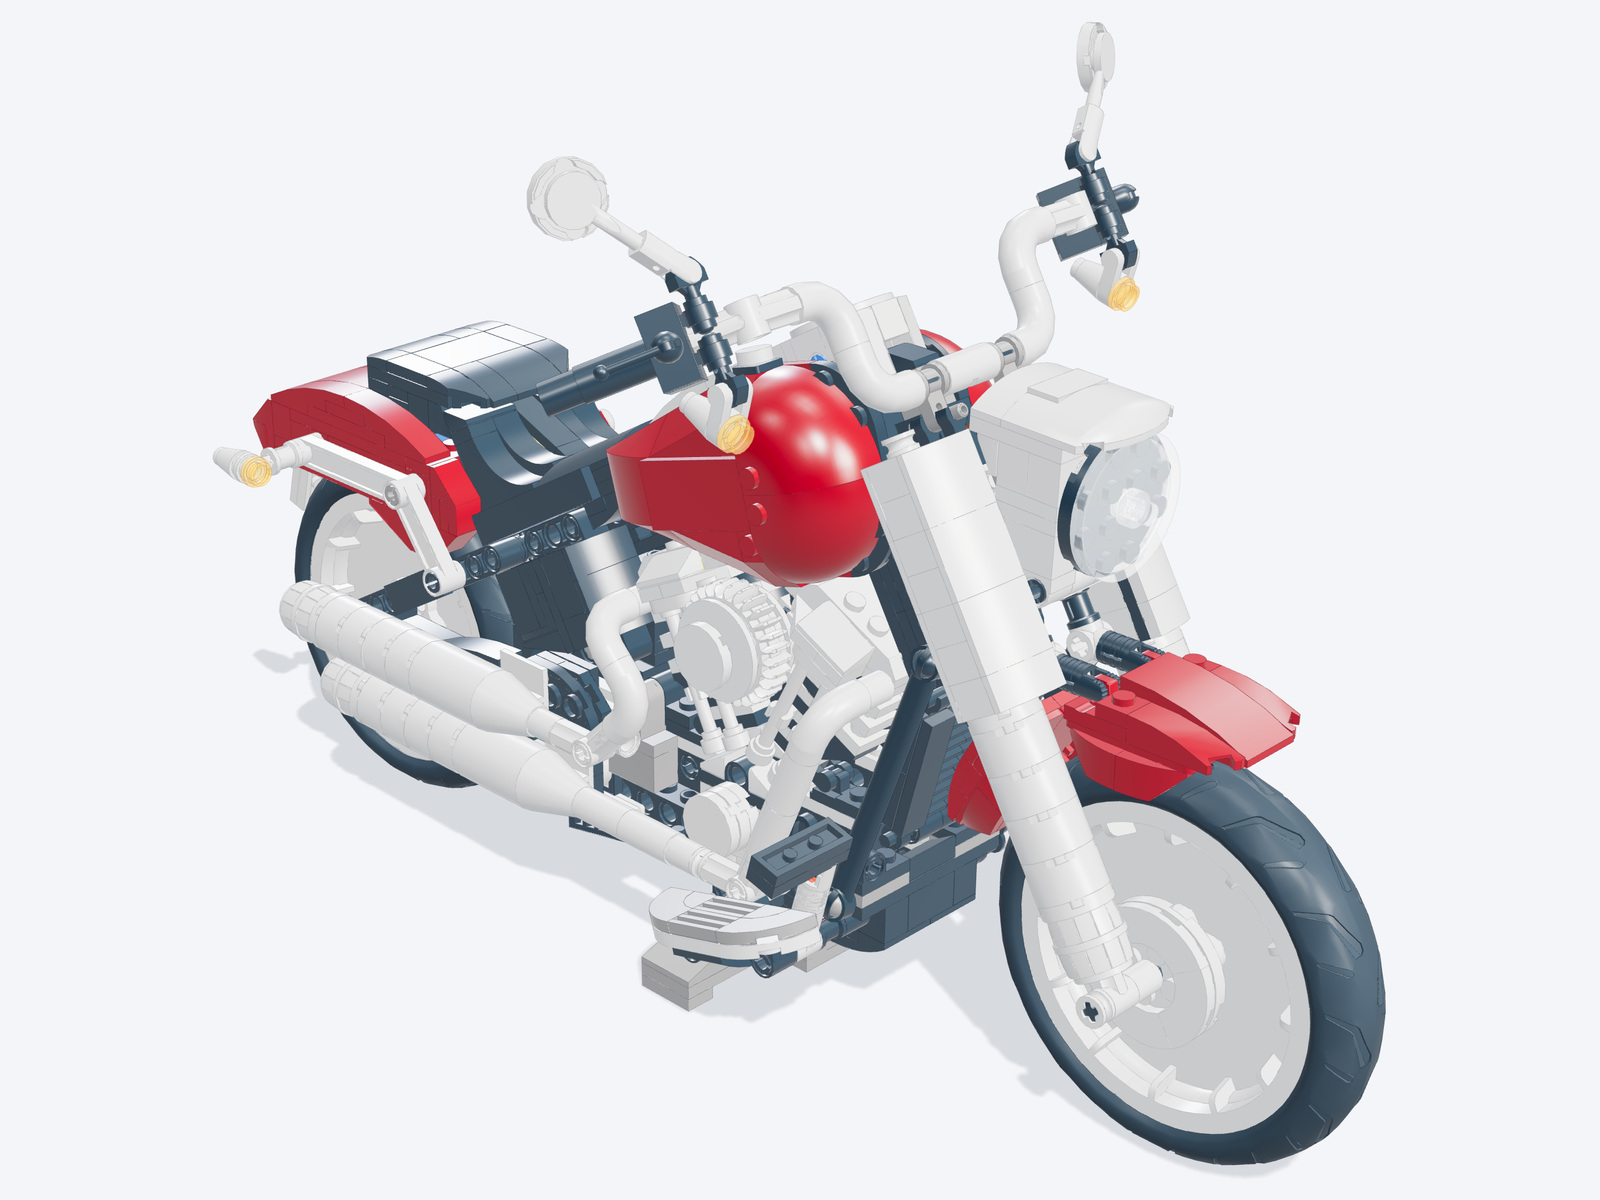
\includegraphics[width=.48\linewidth]{figures/ldraw/print/omr-10269-iso.jpg}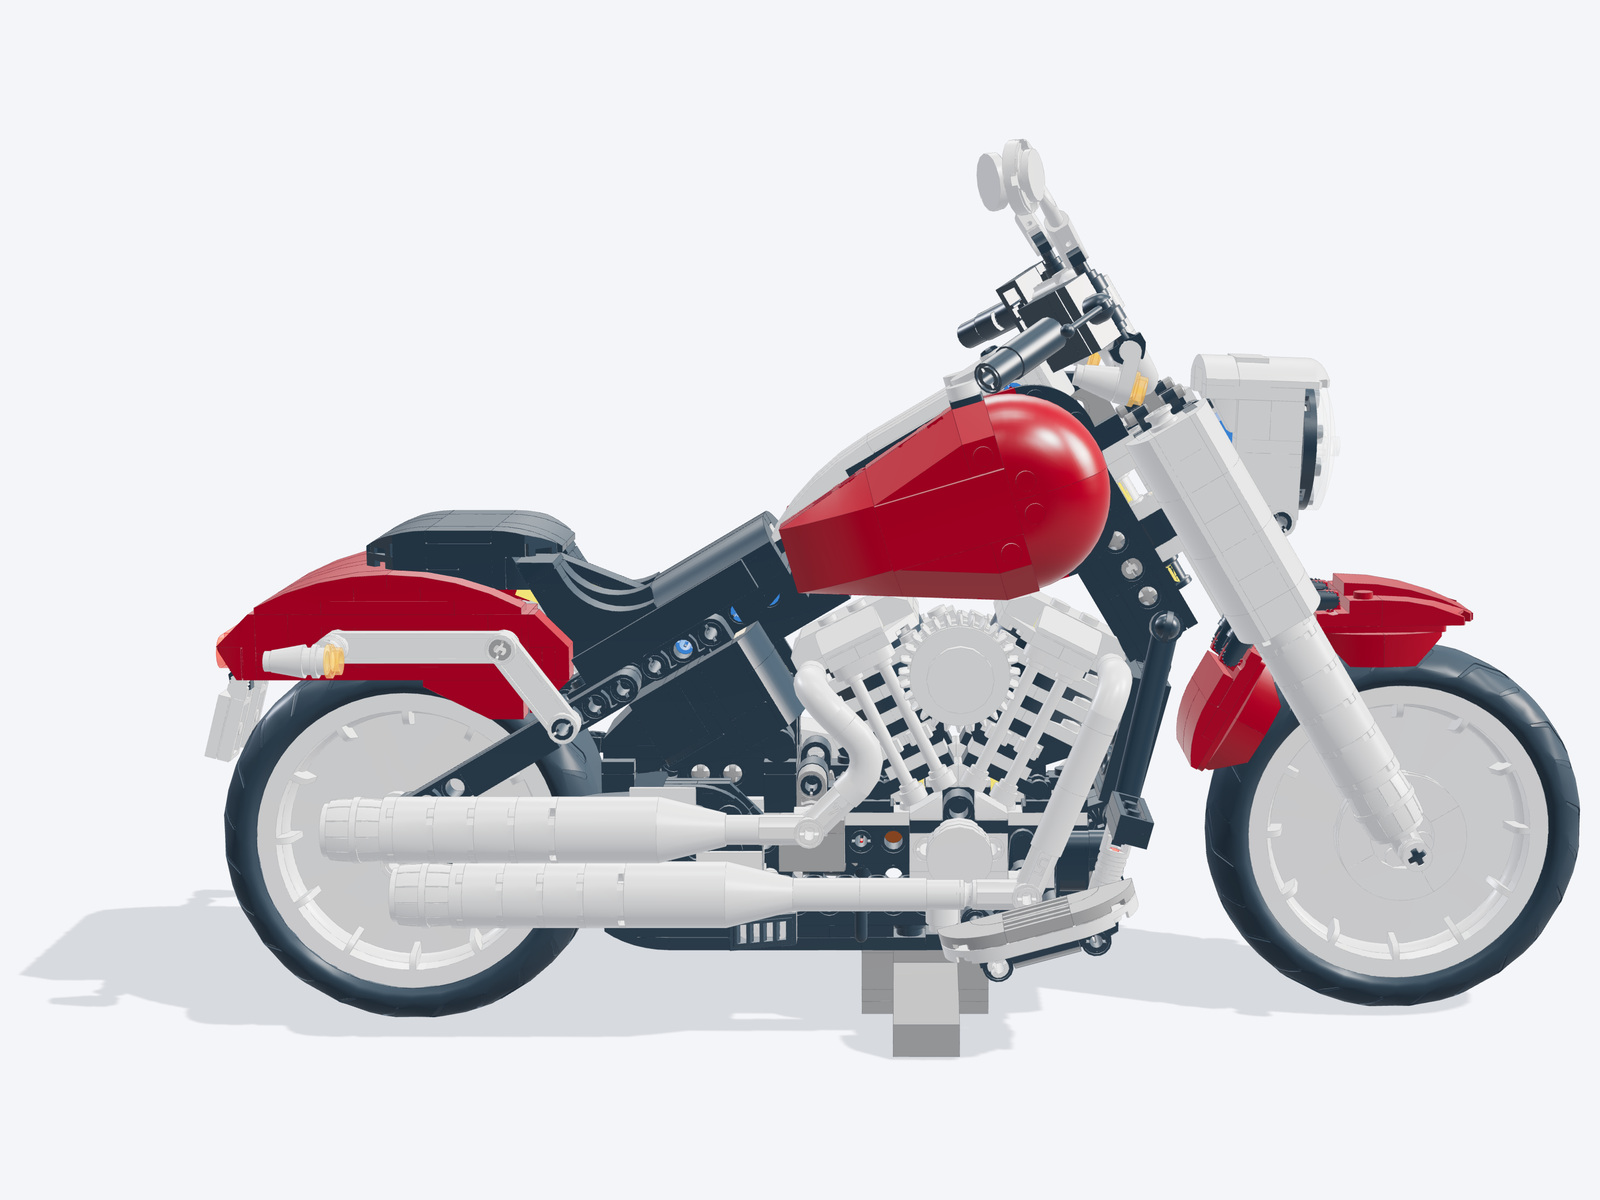
\includegraphics[width=.48\linewidth]{figures/ldraw/print/omr-10269-front.jpg}\\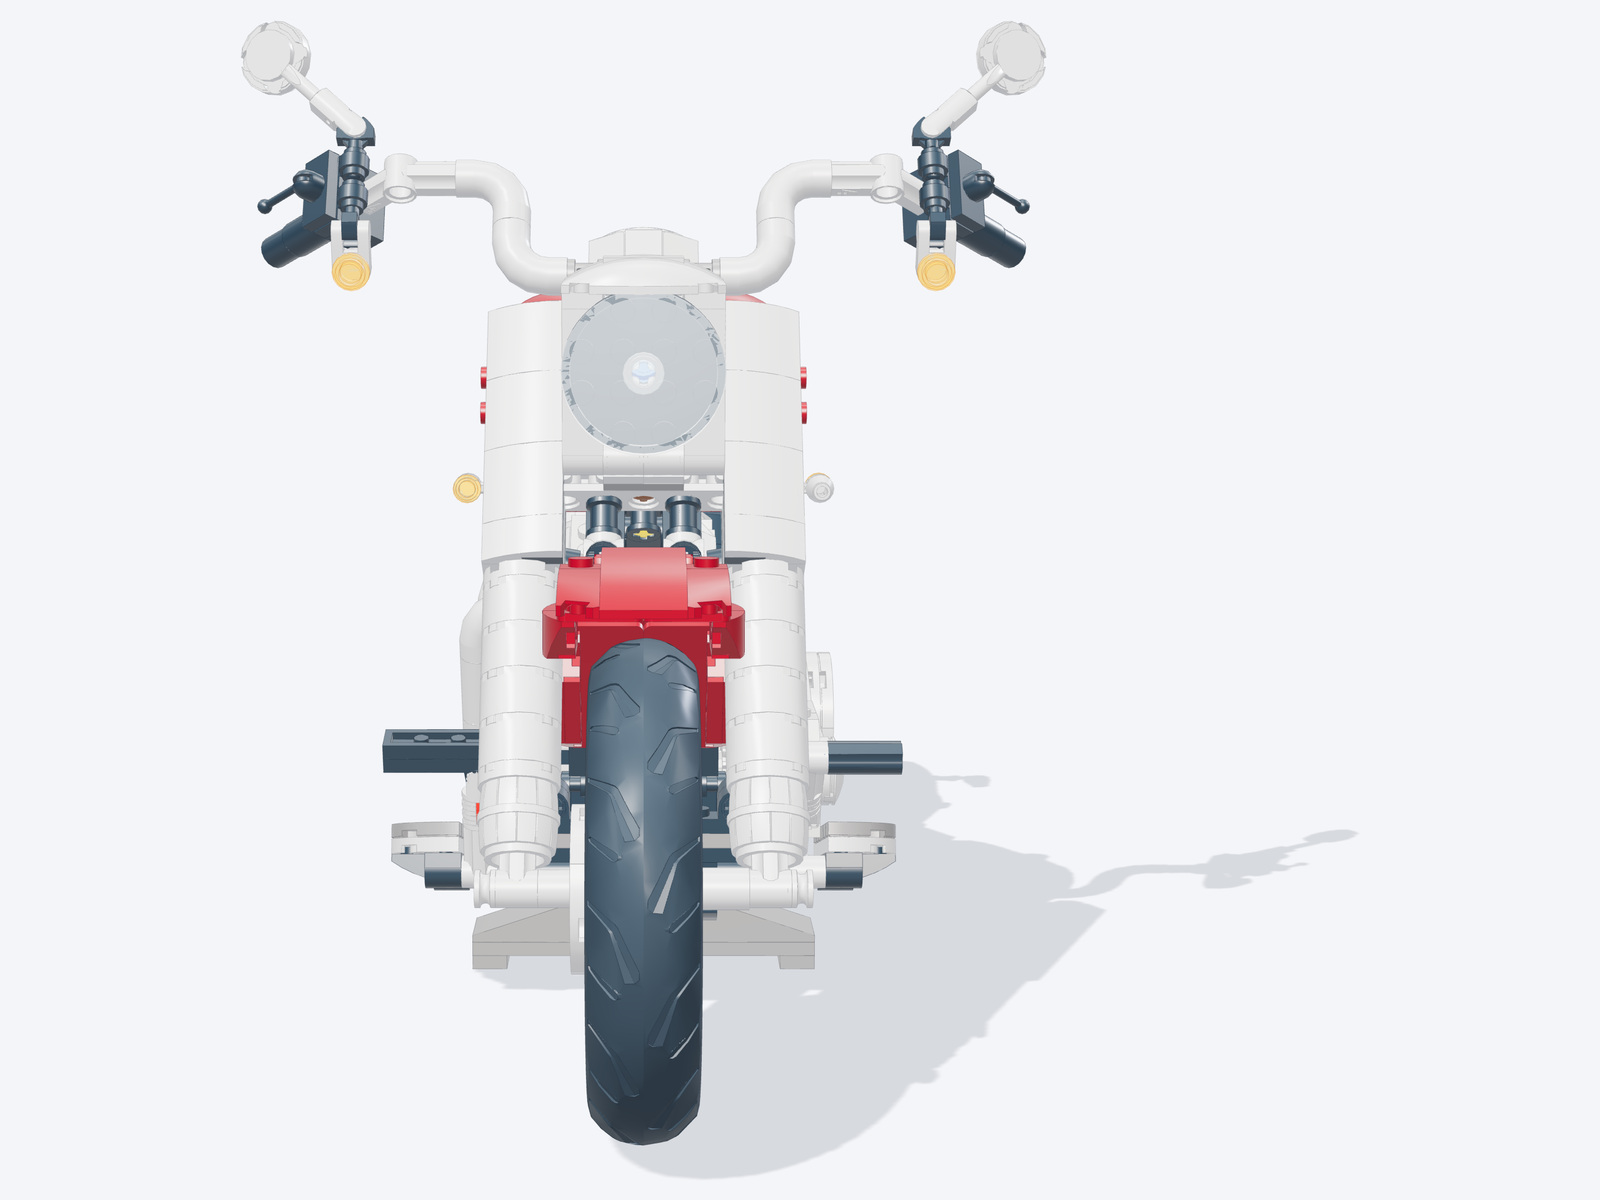
\includegraphics[width=.48\linewidth]{figures/ldraw/print/omr-10269-side.jpg}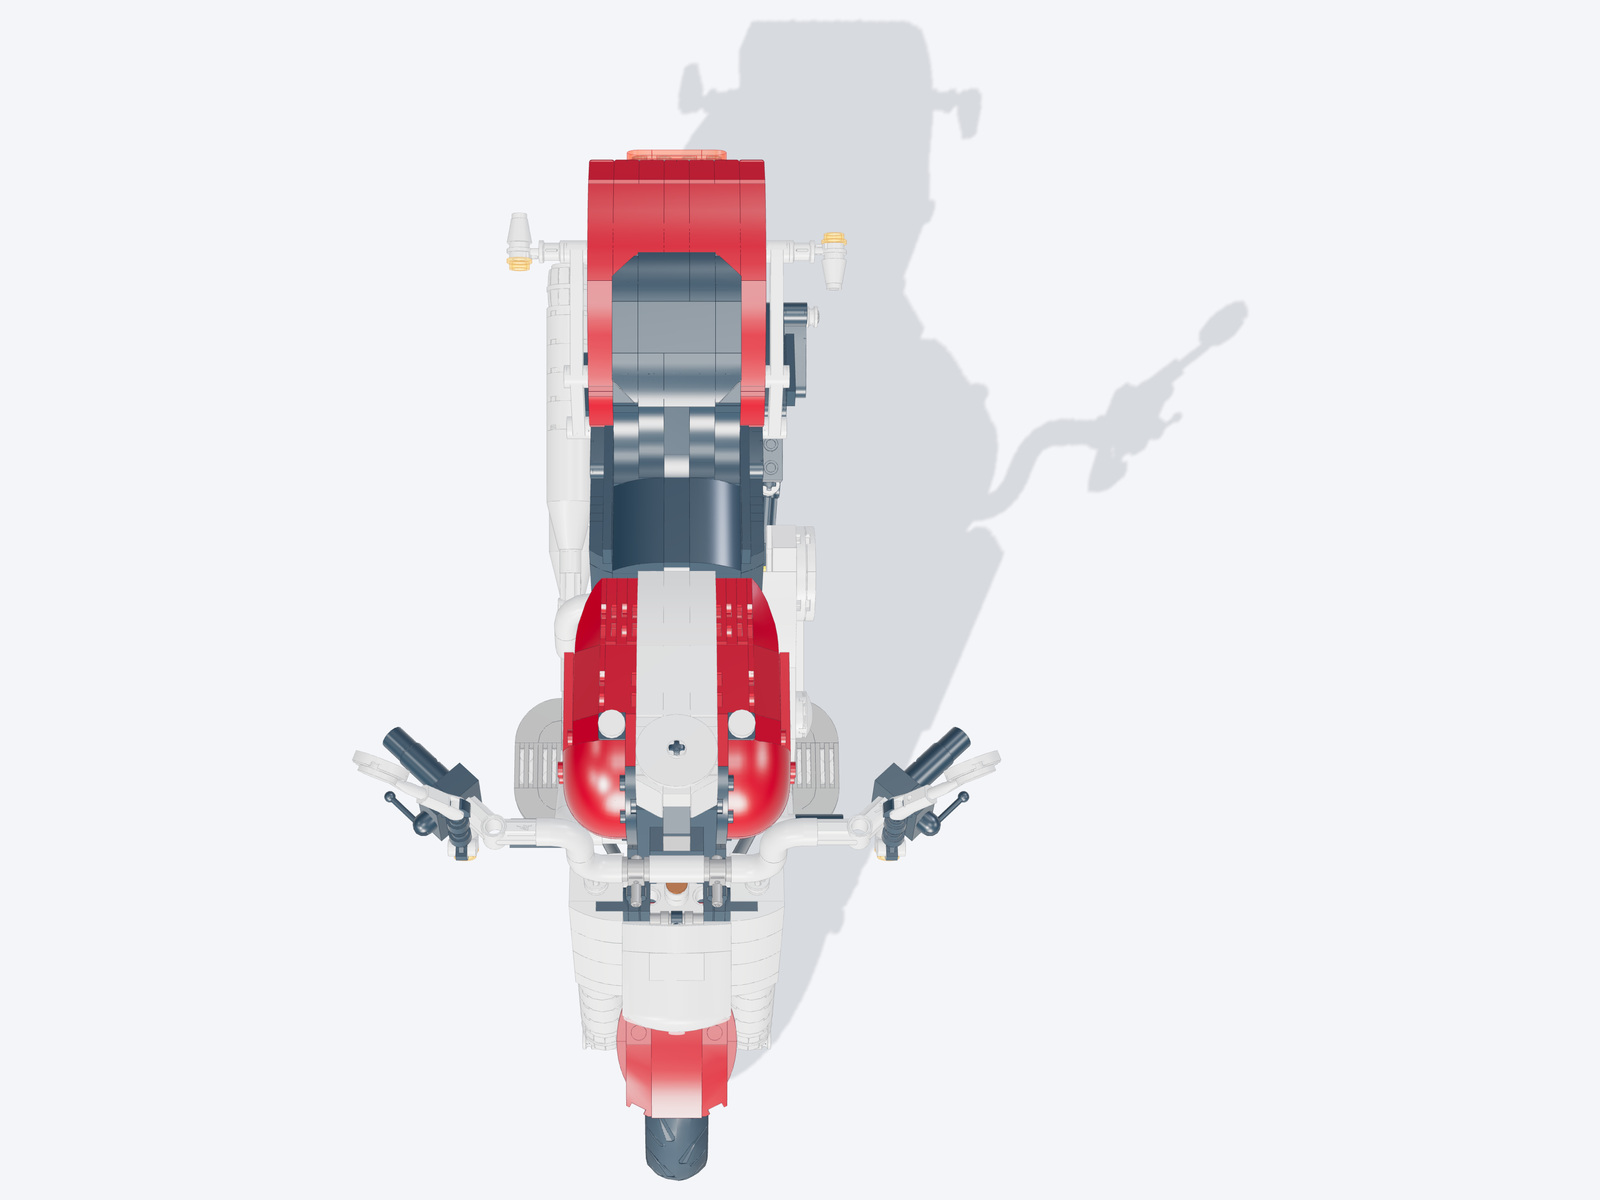
\includegraphics[width=.48\linewidth]{figures/ldraw/print/omr-10269-top.jpg}\end{center}
\paragraph{Attribution.}Orion Pobursky [OrionP]. CC BY 2.0.\par\noindent\url{https://library.ldraw.org/library/omr/10269-1.mpd}
\paragraph{Source lock.}\small\texttt{777f57f34cc8f4bddcee0ff94d81bfef}\\\texttt{d615b7ad4e92ab668cedb66d4b29f476}\normalsize
\paragraph{Evidence coverage.}Connector definitions cover 98.83\% of instances. The audit reports 23 recognized-graph components and 40 intersection candidates without a recognized mating pair. 12 instances have no connector definition. These counts do not certify physical defects or gravitational stability.
\paragraph{Instructions.}340 expanded author steps.
\clearpage\subsection{Numbered visual input and complete question index}
Only relevant numbers are shown. The website can isolate any instance; public visual tasks provide their own numbered images. The following entries give every English prompt, all choice options, compact public evidence and the reference output. Raw repeated connector records and full action fact sets remain in the versioned JSON.
\begin{center}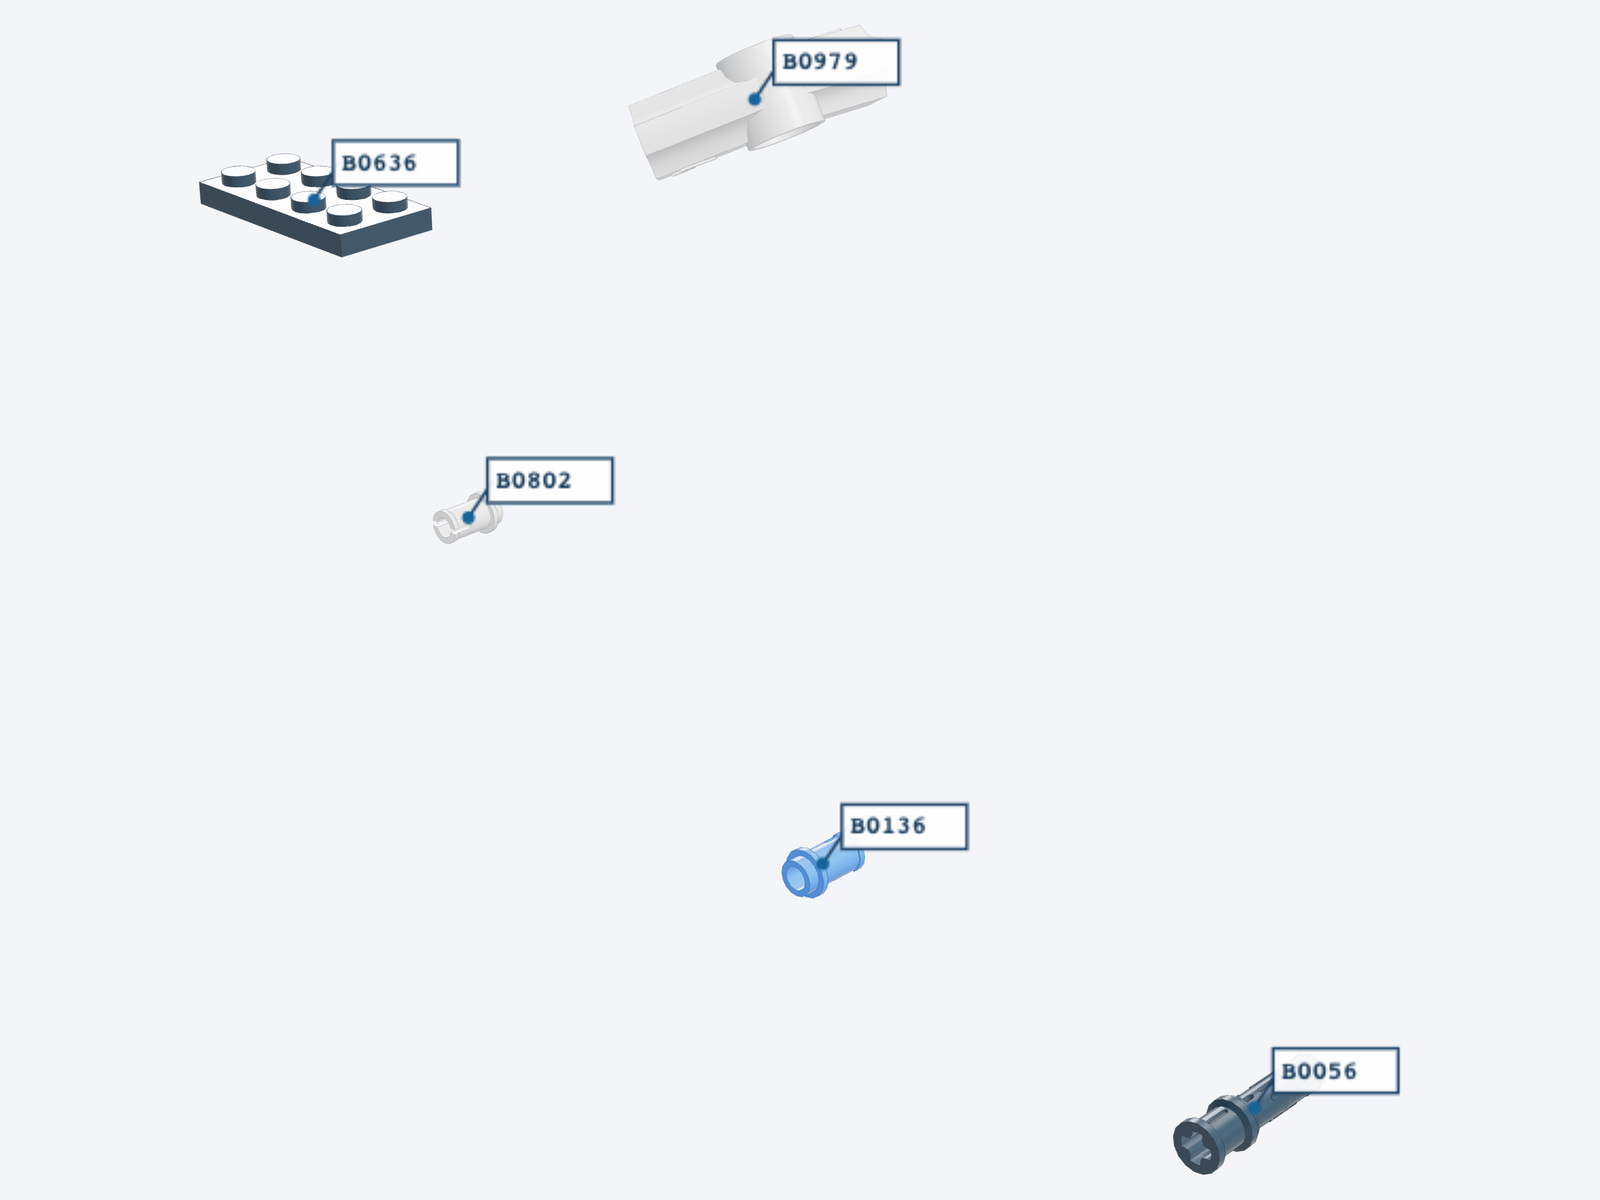
\includegraphics[width=.55\linewidth]{figures/ldraw/print/omr-10269-numbered.jpg}\end{center}
\begin{enumerate}
\item \textbf{color-1}. Identify the original color of B0802; numbered isolation is allowed.\par {\small \textit{Input:} Numbered visual input; source attributes are withheld from the model. \par\textit{Options:} A: Reddish Brown; B: Light Bluish Grey; C: Sand Blue; D: Rubber Black. \par\textit{Reference output:} B.}
\item \textbf{shape-match-1}. Ignoring color and pose, which numbered instance has the same LDraw part type as B0802?\par {\small \textit{Input:} Numbered visual input; source attributes are withheld from the model. \par\textit{Options:} A: B0979; B: B0056; C: B0136; D: B0636. \par\textit{Reference output:} C.}
\item \textbf{distance-1}. Using the supplied geometry bounding-box centers, which candidate is nearest to B0802?\par {\small \textit{Input:} Centers (mm): B0802 = (32.8, 64.264, -107.36); B0407 = (24, 58.380604, -65.432031); B0950 = (12, 149.6982, 72.237453); B0796 = (-48, 29.1214, 10.6146). \par\textit{Options:} A: B0796; B: B0407; C: B0950. \par\textit{Reference output:} B.}
\item \textbf{color-2}. Identify the original color of B0626; numbered isolation is allowed.\par {\small \textit{Input:} Numbered visual input; source attributes are withheld from the model. \par\textit{Options:} A: Yellow; B: Dark Bluish Grey; C: Trans Red; D: Dark Red. \par\textit{Reference output:} A.}
\item \textbf{shape-match-2}. Ignoring color and pose, which numbered instance has the same LDraw part type as B0626?\par {\small \textit{Input:} Numbered visual input; source attributes are withheld from the model. \par\textit{Options:} A: B0405; B: B0474; C: B0970; D: B0359. \par\textit{Reference output:} B.}
\item \textbf{distance-2}. Using the supplied geometry bounding-box centers, which candidate is nearest to B0626?\par {\small \textit{Input:} Centers (mm): B0626 = (0, 133.4356, -8.7248); B0388 = (24, 26.5669, -98.571706); B0911 = (12, 44.1108, 118.6532); B0492 = (20, 95.7316, -99.5424). \par\textit{Options:} A: B0911; B: B0492; C: B0388. \par\textit{Reference output:} B.}
\item \textbf{color-3}. Identify the original color of B0487; numbered isolation is allowed.\par {\small \textit{Input:} Numbered visual input; source attributes are withheld from the model. \par\textit{Options:} A: Dark Red; B: Light Bluish Grey; C: Blue; D: Black. \par\textit{Reference output:} A.}
\item \textbf{shape-match-3}. Ignoring color and pose, which numbered instance has the same LDraw part type as B0487?\par {\small \textit{Input:} Numbered visual input; source attributes are withheld from the model. \par\textit{Options:} A: B0483; B: B0586; C: B0255; D: B0608. \par\textit{Reference output:} A.}
\item \textbf{distance-3}. Using the supplied geometry bounding-box centers, which candidate is nearest to B0487?\par {\small \textit{Input:} Centers (mm): B0487 = (4, 108.5316, -129.1424); B0317 = (8, 95.208418, 52.719016); B0242 = (0, 98.6624, 21.9632); B0865 = (-24, 141.1188, 61.0124). \par\textit{Options:} A: B0242; B: B0865; C: B0317. \par\textit{Reference output:} A.}
\item \textbf{color-4}. Identify the original color of B0033; numbered isolation is allowed.\par {\small \textit{Input:} Numbered visual input; source attributes are withheld from the model. \par\textit{Options:} A: Light Bluish Grey; B: Red; C: Dark Bluish Grey; D: Trans Orange. \par\textit{Reference output:} A.}
\item \textbf{shape-match-4}. Ignoring color and pose, which numbered instance has the same LDraw part type as B0033?\par {\small \textit{Input:} Numbered visual input; source attributes are withheld from the model. \par\textit{Options:} A: B0990; B: B0685; C: B0314; D: B0468. \par\textit{Reference output:} D.}
\item \textbf{distance-4}. Using the supplied geometry bounding-box centers, which candidate is nearest to B0033?\par {\small \textit{Input:} Centers (mm): B0033 = (20, 28, 12); B0003 = (12, 21.6, -60); B0374 = (-8, 120.2692, 26.2124); B0147 = (-12, 34.4, 28). \par\textit{Options:} A: B0003; B: B0147; C: B0374. \par\textit{Reference output:} B.}
\item \textbf{interface-1}. Classify the supplied connector record for B0090 and B0091. This does not certify load capacity.\par {\small \textit{Input:} Record: family = axle; connector indices = 22, 1. \par\textit{Options:} A: fixed; B: ball; C: hinge; D: axle. \par\textit{Reference output:} D.}
\item \textbf{interface-2}. Classify the supplied connector record for B0045 and B0433. This does not certify load capacity.\par {\small \textit{Input:} Record: family = ball; connector indices = 3, 0. \par\textit{Options:} A: fixed; B: ball; C: axle; D: hinge. \par\textit{Reference output:} B.}
\item \textbf{interface-3}. Classify the supplied connector record for B0384 and B0383. This does not certify load capacity.\par {\small \textit{Input:} Record: family = hinge; connector indices = 0, 1. \par\textit{Options:} A: axle; B: fixed; C: ball; D: hinge. \par\textit{Reference output:} D.}
\item \textbf{interface-4}. Classify the supplied connector record for B0454 and B0456. This does not certify load capacity.\par {\small \textit{Input:} Record: family = stud; connector indices = 10, 2. \par\textit{Options:} A: stud; B: hinge; C: fixed; D: axle; E: ball. \par\textit{Reference output:} A.}
\item \textbf{neighbors-1}. Select every candidate directly adjacent to B0282 in the supplied connector graph.\par {\small \textit{Input:} Unique undirected pairs: B0265 / B0282; B0280 / B0282; B0282 / B0283; B0282 / B0284. \par\textit{Options:} A: B0618; B: B0284; C: B0413; D: B0280; E: B0283; F: B0265. \par\textit{Reference output:} B, D, E, F.}
\item \textbf{graph-removal-1}. Delete B0282 and its incident edges from this local graph. How many connected components remain? Do not infer physical extractability.\par {\small \textit{Input:} Nodes: B0282, B0280, B0284, B0283, B0265, B0413, B0618. Unique undirected pairs: B0265 / B0282; B0280 / B0282; B0282 / B0283; B0282 / B0284. \par\textit{Options:} A: 6; B: 8; C: 7; D: 5. \par\textit{Reference output:} A.}
\item \textbf{neighbors-2}. Select every candidate directly adjacent to B0764 in the supplied connector graph.\par {\small \textit{Input:} Unique undirected pairs: B0762 / B0764; B0763 / B0764; B0763 / B0766; B0764 / B0765; B0764 / B0766. \par\textit{Options:} A: B0422; B: B0765; C: B0766; D: B0053; E: B0762; F: B0763. \par\textit{Reference output:} B, C, E, F.}
\item \textbf{graph-removal-2}. Delete B0764 and its incident edges from this local graph. How many connected components remain? Do not infer physical extractability.\par {\small \textit{Input:} Nodes: B0764, B0766, B0763, B0765, B0762, B0422, B0053. Unique undirected pairs: B0762 / B0764; B0763 / B0764; B0763 / B0766; B0764 / B0765; B0764 / B0766. \par\textit{Options:} A: 5; B: 4; C: 7; D: 6. \par\textit{Reference output:} A.}
\item \textbf{neighbors-3}. Select every candidate directly adjacent to B0973 in the supplied connector graph.\par {\small \textit{Input:} Unique undirected pairs: B0972 / B0973; B0973 / B0975. \par\textit{Options:} A: B0624; B: B0836; C: B0975; D: B0972. \par\textit{Reference output:} C, D.}
\item \textbf{graph-removal-3}. Delete B0973 and its incident edges from this local graph. How many connected components remain? Do not infer physical extractability.\par {\small \textit{Input:} Nodes: B0973, B0972, B0975, B0624, B0836. Unique undirected pairs: B0972 / B0973; B0973 / B0975. \par\textit{Options:} A: 3; B: 4; C: 5; D: 6. \par\textit{Reference output:} B.}
\item \textbf{neighbors-4}. Select every candidate directly adjacent to B0127 in the supplied connector graph.\par {\small \textit{Input:} Unique undirected pairs: B0126 / B0127; B0127 / B0128; B0127 / B0129; B0127 / B0130. \par\textit{Options:} A: B0130; B: B0128; C: B0129; D: B0537; E: B0126; F: B0681. \par\textit{Reference output:} A, B, C, E.}
\item \textbf{graph-removal-4}. Delete B0127 and its incident edges from this local graph. How many connected components remain? Do not infer physical extractability.\par {\small \textit{Input:} Nodes: B0127, B0129, B0126, B0128, B0130, B0537, B0681. Unique undirected pairs: B0126 / B0127; B0127 / B0128; B0127 / B0129; B0127 / B0130. \par\textit{Options:} A: 8; B: 7; C: 5; D: 6. \par\textit{Reference output:} D.}
\item \textbf{coverage-1}. Which numbered instance lacks a connector definition in the coverage record, so this audit cannot establish that it is floating?\par {\small \textit{Input:} Definition coverage: B0256 = unsupported; B0802 = supported; B0626 = supported; B0487 = supported. \par\textit{Options:} A: B0256; B: B0487; C: B0626; D: B0802. \par\textit{Reference output:} A.}
\item \textbf{evidence-limit-1}. Only source geometry, connector matching and mesh intersection audits are available. Without mass, friction, material or dynamic tests, is gravitational stability established?\par {\small \textit{Input:} Available evidence: Original CAD; Connector inference; Inset-mesh intersection candidates. \par\textit{Options:} A: Not established by this evidence; B: Established. \par\textit{Reference output:} A.}
\item \textbf{source-step-1}. At which expanded author step does B0533 first appear in the supplied source-step table? Source order is not a collision-free assembly proof.\par {\small \textit{Input:} Expanded author records: step 1: B0001; step 152: B0533. \par\textit{Options:} A: 154; B: 152; C: 153; D: 151. \par\textit{Reference output:} B.}
\item \textbf{source-step-2}. At which expanded author step does B0037 first appear in the supplied source-step table? Source order is not a collision-free assembly proof.\par {\small \textit{Input:} Expanded author records: step 1: B0001; step 10: B0037. \par\textit{Options:} A: 12; B: 9; C: 10; D: 11. \par\textit{Reference output:} C.}
\item \textbf{source-step-3}. At which expanded author step does B0667 first appear in the supplied source-step table? Source order is not a collision-free assembly proof.\par {\small \textit{Input:} Expanded author records: step 1: B0001; step 204: B0667. \par\textit{Options:} A: 206; B: 205; C: 204; D: 203. \par\textit{Reference output:} C.}
\item \textbf{source-step-4}. At which expanded author step does B0767 first appear in the supplied source-step table? Source order is not a collision-free assembly proof.\par {\small \textit{Input:} Expanded author records: step 1: B0001; step 243: B0767. \par\textit{Options:} A: 245; B: 242; C: 244; D: 243. \par\textit{Reference output:} D.}
\item \textbf{source-sequence-1}. Reveal the supplied source-step window in author order. Actions change visibility only, without simulating insertion trajectories.\par {\small \textit{Input:} Source window: step-1: B0001, B0002, B0003; step-2: B0004, B0005, B0006, B0007, B0008; step-3: B0009, B0010; step-4: B0011, B0012, B0013, B0014, B0015, B0016; step-5: B0017, B0018, B0019, B0020; step-6: B0021, B0022, B0023. Action budget: 6. \par\textit{Reference output:} step-1, step-2, step-3, step-4, step-5, step-6.}
\item \textbf{restore-instance-1}. The display copy hides B0802. Restore only that numbered instance, preserving all other instances and source poses.\par {\small \textit{Input:} Target: B0802. Action budget: 1. All other instances initially remain visible. \par\textit{Reference output:} restore-B0802.}
\item \textbf{restore-instance-2}. The display copy hides B0626. Restore only that numbered instance, preserving all other instances and source poses.\par {\small \textit{Input:} Target: B0626. Action budget: 1. All other instances initially remain visible. \par\textit{Reference output:} restore-B0626.}
\item \textbf{restore-instance-3}. The display copy hides B0487. Restore only that numbered instance, preserving all other instances and source poses.\par {\small \textit{Input:} Target: B0487. Action budget: 1. All other instances initially remain visible. \par\textit{Reference output:} restore-B0487.}
\end{enumerate}
\clearpage
\section{10242: MINI Cooper}
1086 source instances; 34 tasks; D4 scale band.

\par\noindent Perspective, front, side and top views follow in reading order. Original source transforms are preserved.
\begin{center}
\includegraphics[width=.48\linewidth]{figures/ldraw/print/omr-10242-iso.jpg}
\includegraphics[width=.48\linewidth]{figures/ldraw/print/omr-10242-front.jpg}\\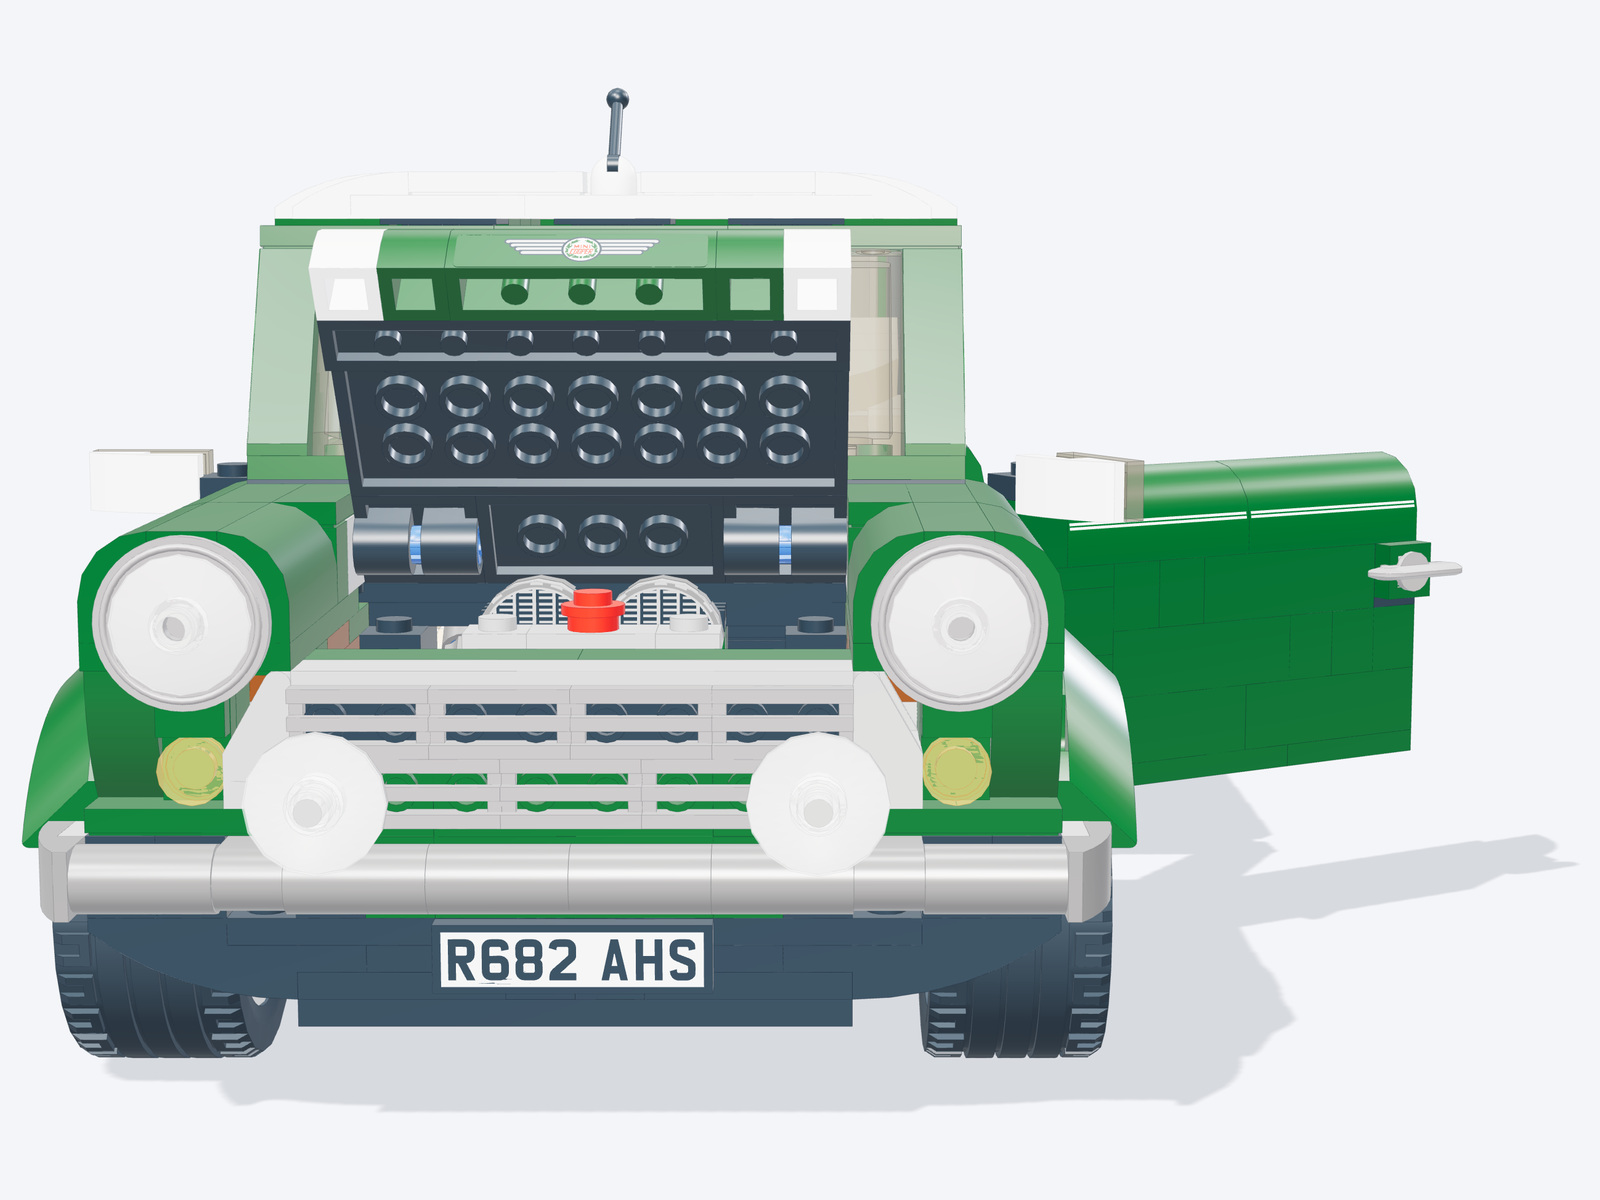
\includegraphics[width=.48\linewidth]{figures/ldraw/print/omr-10242-side.jpg}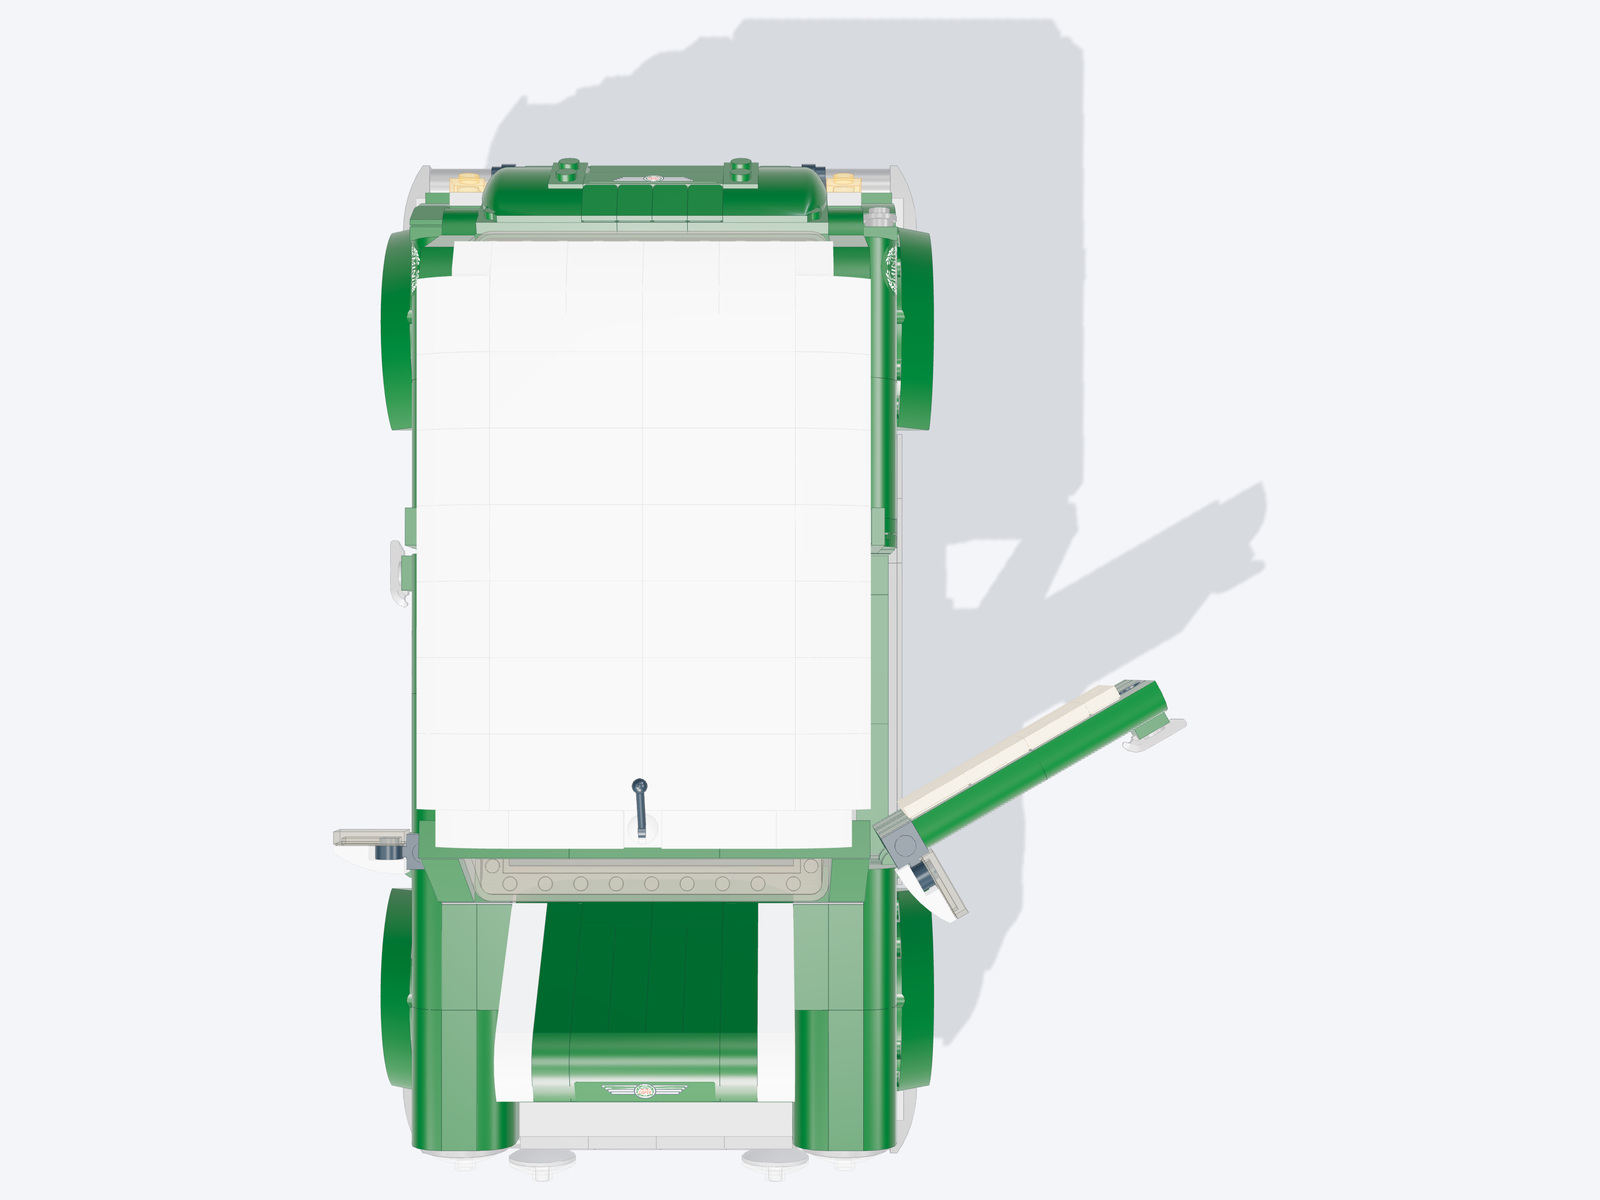
\includegraphics[width=.48\linewidth]{figures/ldraw/print/omr-10242-top.jpg}\end{center}
\paragraph{Attribution.}Magnus Forsberg [MagFors]. CC BY 2.0.\par\noindent\url{https://library.ldraw.org/library/omr/10242-1.mpd}
\paragraph{Source lock.}\small\texttt{d79fd06503b145cc5ff3c5bcfe71a1c4}\\\texttt{02910dee78424f54077faba9cf402b74}\normalsize
\paragraph{Evidence coverage.}Connector definitions cover 99.08\% of instances. The audit reports 18 recognized-graph components and 17 intersection candidates without a recognized mating pair. 10 instances have no connector definition. These counts do not certify physical defects or gravitational stability.
\paragraph{Instructions.}233 expanded author steps.
\clearpage\subsection{Numbered visual input and complete question index}
Only relevant numbers are shown. The website can isolate any instance; public visual tasks provide their own numbered images. The following entries give every English prompt, all choice options, compact public evidence and the reference output. Raw repeated connector records and full action fact sets remain in the versioned JSON.
\begin{center}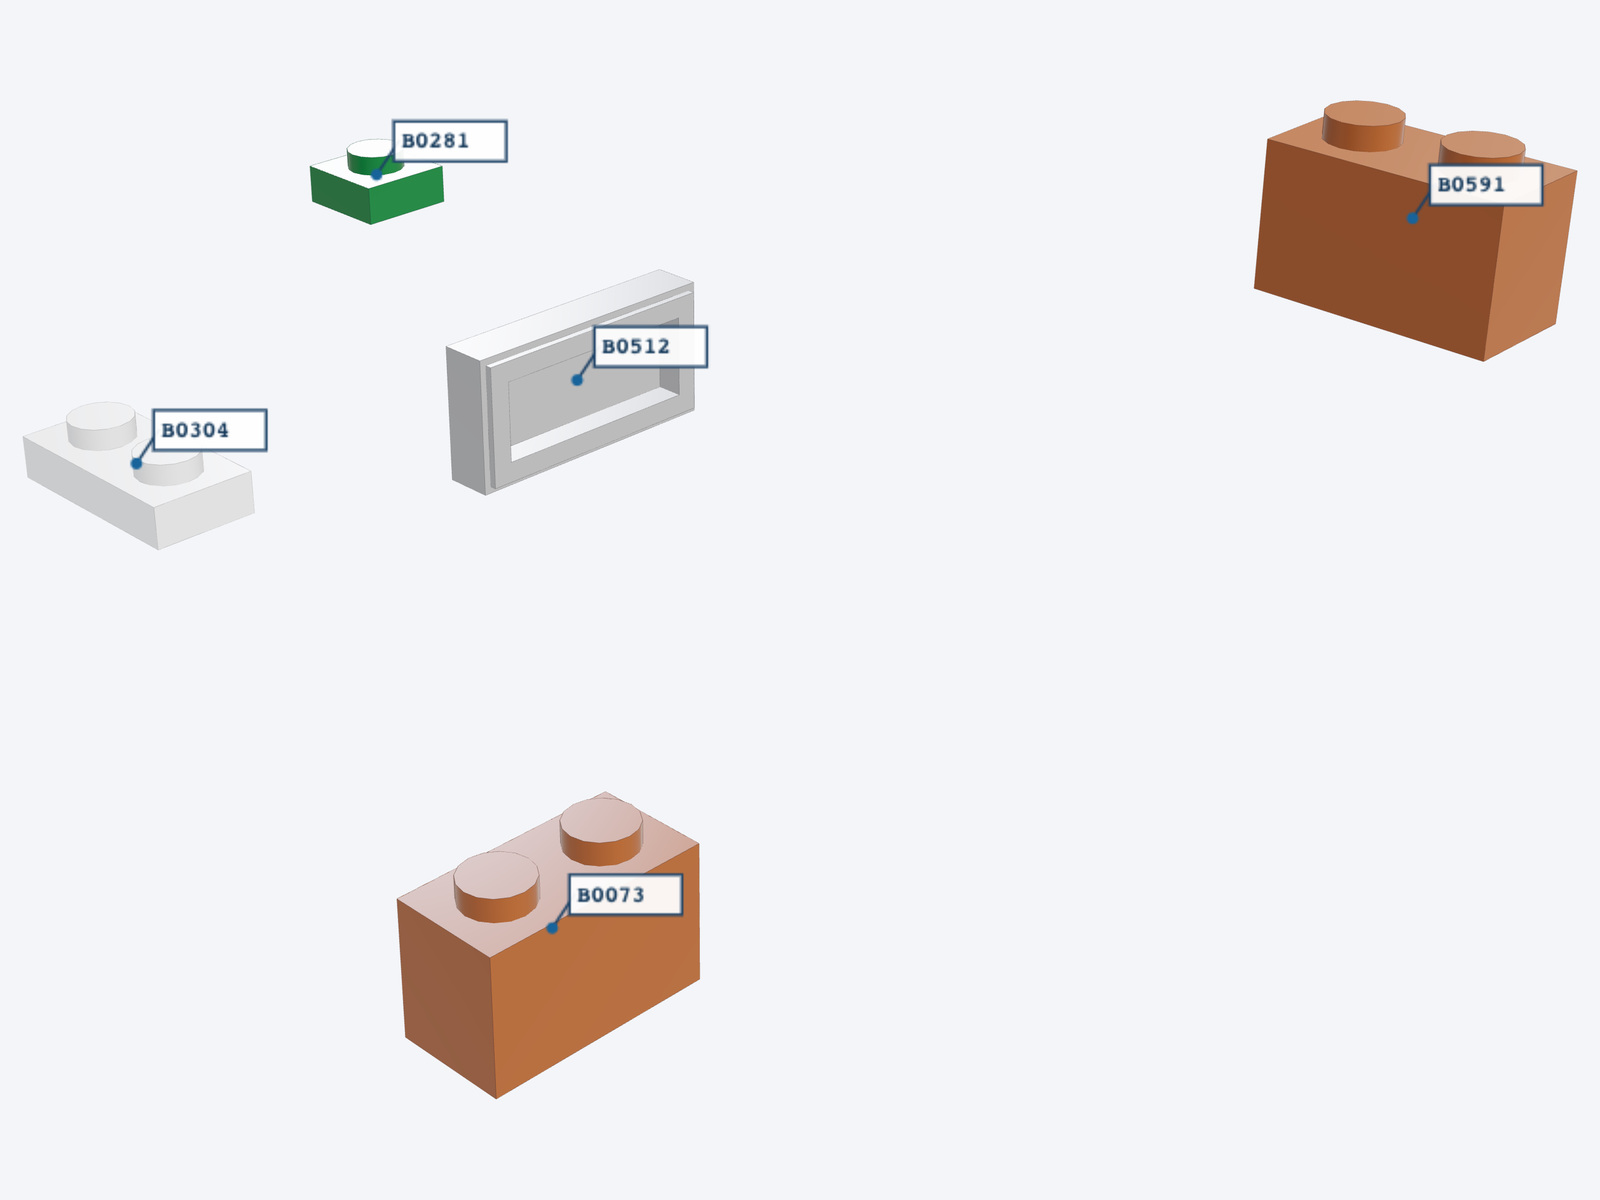
\includegraphics[width=.55\linewidth]{figures/ldraw/print/omr-10242-numbered.jpg}\end{center}
\begin{enumerate}
\item \textbf{color-1}. Identify the original color of B0591; numbered isolation is allowed.\par {\small \textit{Input:} Numbered visual input; source attributes are withheld from the model. \par\textit{Options:} A: White; B: Pearl Gold; C: Reddish Brown; D: Trans Light Blue. \par\textit{Reference output:} C.}
\item \textbf{shape-match-1}. Ignoring color and pose, which numbered instance has the same LDraw part type as B0591?\par {\small \textit{Input:} Numbered visual input; source attributes are withheld from the model. \par\textit{Options:} A: B0073; B: B0304; C: B0512; D: B0281. \par\textit{Reference output:} A.}
\item \textbf{distance-1}. Using the supplied geometry bounding-box centers, which candidate is nearest to B0591?\par {\small \textit{Input:} Centers (mm): B0591 = (44, 34.4, 64); B0669 = (-12, 20.726885, 90.813115); B0950 = (60.928, 31.2, 42.122316); B0840 = (8, 24.059068, -4.9024). \par\textit{Options:} A: B0840; B: B0669; C: B0950. \par\textit{Reference output:} C.}
\item \textbf{color-2}. Identify the original color of B0837; numbered isolation is allowed.\par {\small \textit{Input:} Numbered visual input; source attributes are withheld from the model. \par\textit{Options:} A: Tan; B: Yellow; C: Trans Clear; D: White. \par\textit{Reference output:} A.}
\item \textbf{shape-match-2}. Ignoring color and pose, which numbered instance has the same LDraw part type as B0837?\par {\small \textit{Input:} Numbered visual input; source attributes are withheld from the model. \par\textit{Options:} A: B0303; B: B0845; C: B0166; D: B0341. \par\textit{Reference output:} A.}
\item \textbf{distance-2}. Using the supplied geometry bounding-box centers, which candidate is nearest to B0837?\par {\small \textit{Input:} Centers (mm): B0837 = (40, 31.6984, -0.1184); B0465 = (-36, 21.6, 44); B0511 = (0, 37.6, 38.4); B0103 = (0, 5.6, 116). \par\textit{Options:} A: B0465; B: B0511; C: B0103. \par\textit{Reference output:} B.}
\item \textbf{color-3}. Identify the original color of B0962; numbered isolation is allowed.\par {\small \textit{Input:} Numbered visual input; source attributes are withheld from the model. \par\textit{Options:} A: Bright Light Orange; B: Medium Nougat; C: Trans Brown; D: Black. \par\textit{Reference output:} D.}
\item \textbf{shape-match-3}. Ignoring color and pose, which numbered instance has the same LDraw part type as B0962?\par {\small \textit{Input:} Numbered visual input; source attributes are withheld from the model. \par\textit{Options:} A: B0111; B: B0610; C: B0969; D: B0654. \par\textit{Reference output:} D.}
\item \textbf{distance-3}. Using the supplied geometry bounding-box centers, which candidate is nearest to B0962?\par {\small \textit{Input:} Centers (mm): B0962 = (58.7176, 44, 45.1072); B0714 = (36, 21.6, -60); B0029 = (24, -4, -40); B0312 = (-36, 24.8, -80). \par\textit{Options:} A: B0029; B: B0714; C: B0312. \par\textit{Reference output:} A.}
\item \textbf{color-4}. Identify the original color of B0975; numbered isolation is allowed.\par {\small \textit{Input:} Numbered visual input; source attributes are withheld from the model. \par\textit{Options:} A: Yellow; B: Trans Brown; C: Dark Green; D: Medium Nougat. \par\textit{Reference output:} C.}
\item \textbf{shape-match-4}. Ignoring color and pose, which numbered instance has the same LDraw part type as B0975?\par {\small \textit{Input:} Numbered visual input; source attributes are withheld from the model. \par\textit{Options:} A: B0180; B: B1004; C: B0657; D: B0485. \par\textit{Reference output:} D.}
\item \textbf{distance-4}. Using the supplied geometry bounding-box centers, which candidate is nearest to B0975?\par {\small \textit{Input:} Centers (mm): B0975 = (-51.2, 28, 28); B0857 = (24, 59.534, 21.9088); B0379 = (-40, 37.6, -68); B0265 = (48, 5.6, -44). \par\textit{Options:} A: B0857; B: B0379; C: B0265. \par\textit{Reference output:} A.}
\item \textbf{interface-1}. Classify the supplied connector record for B0028 and B0032. This does not certify load capacity.\par {\small \textit{Input:} Record: family = axle; connector indices = 12, 0. \par\textit{Options:} A: ball; B: axle; C: fixed; D: hinge. \par\textit{Reference output:} B.}
\item \textbf{interface-2}. Classify the supplied connector record for B0153 and B0154. This does not certify load capacity.\par {\small \textit{Input:} Record: family = fixed; connector indices = 1, 1. \par\textit{Options:} A: ball; B: fixed; C: hinge; D: axle. \par\textit{Reference output:} B.}
\item \textbf{interface-3}. Classify the supplied connector record for B0578 and B0981. This does not certify load capacity.\par {\small \textit{Input:} Record: family = hinge; connector indices = 1, 2. \par\textit{Options:} A: ball; B: axle; C: fixed; D: hinge. \par\textit{Reference output:} D.}
\item \textbf{interface-4}. Classify the supplied connector record for B1027 and B1034. This does not certify load capacity.\par {\small \textit{Input:} Record: family = stud; connector indices = 203, 5. \par\textit{Options:} A: fixed; B: hinge; C: ball; D: stud; E: axle. \par\textit{Reference output:} D.}
\item \textbf{neighbors-1}. Select every candidate directly adjacent to B0732 in the supplied connector graph.\par {\small \textit{Input:} Unique undirected pairs: B0380 / B0732; B0720 / B0732; B0729 / B0733; B0732 / B0733. \par\textit{Options:} A: B0380; B: B0733; C: B0550; D: B0720; E: B0729. \par\textit{Reference output:} A, B, D.}
\item \textbf{graph-removal-1}. Delete B0732 and its incident edges from this local graph. How many connected components remain? Do not infer physical extractability.\par {\small \textit{Input:} Nodes: B0732, B0733, B0380, B0720, B0550, B0729. Unique undirected pairs: B0380 / B0732; B0720 / B0732; B0729 / B0733; B0732 / B0733. \par\textit{Options:} A: 6; B: 5; C: 3; D: 4. \par\textit{Reference output:} D.}
\item \textbf{neighbors-2}. Select every candidate directly adjacent to B0711 in the supplied connector graph.\par {\small \textit{Input:} Unique undirected pairs: B0679 / B0711; B0711 / B0719. \par\textit{Options:} A: B0030; B: B0719; C: B0469; D: B0679. \par\textit{Reference output:} B, D.}
\item \textbf{graph-removal-2}. Delete B0711 and its incident edges from this local graph. How many connected components remain? Do not infer physical extractability.\par {\small \textit{Input:} Nodes: B0711, B0719, B0679, B0030, B0469. Unique undirected pairs: B0679 / B0711; B0711 / B0719. \par\textit{Options:} A: 3; B: 5; C: 4; D: 6. \par\textit{Reference output:} C.}
\item \textbf{neighbors-3}. Select every candidate directly adjacent to B0074 in the supplied connector graph.\par {\small \textit{Input:} Unique undirected pairs: B0043 / B0074; B0074 / B0231; B0074 / B0294. \par\textit{Options:} A: B0231; B: B0043; C: B0704; D: B0349; E: B0294. \par\textit{Reference output:} A, B, E.}
\item \textbf{graph-removal-3}. Delete B0074 and its incident edges from this local graph. How many connected components remain? Do not infer physical extractability.\par {\small \textit{Input:} Nodes: B0074, B0294, B0231, B0043, B0704, B0349. Unique undirected pairs: B0043 / B0074; B0074 / B0231; B0074 / B0294. \par\textit{Options:} A: 6; B: 7; C: 5; D: 4. \par\textit{Reference output:} C.}
\item \textbf{neighbors-4}. Select every candidate directly adjacent to B0402 in the supplied connector graph.\par {\small \textit{Input:} Unique undirected pairs: B0384 / B0402; B0402 / B0415. \par\textit{Options:} A: B0384; B: B0188; C: B0917; D: B0415. \par\textit{Reference output:} A, D.}
\item \textbf{graph-removal-4}. Delete B0402 and its incident edges from this local graph. How many connected components remain? Do not infer physical extractability.\par {\small \textit{Input:} Nodes: B0402, B0415, B0384, B0188, B0917. Unique undirected pairs: B0384 / B0402; B0402 / B0415. \par\textit{Options:} A: 5; B: 3; C: 4; D: 6. \par\textit{Reference output:} C.}
\item \textbf{coverage-1}. Which numbered instance lacks a connector definition in the coverage record, so this audit cannot establish that it is floating?\par {\small \textit{Input:} Definition coverage: B0014 = unsupported; B0591 = supported; B0837 = supported; B0962 = supported. \par\textit{Options:} A: B0962; B: B0014; C: B0591; D: B0837. \par\textit{Reference output:} B.}
\item \textbf{evidence-limit-1}. Only source geometry, connector matching and mesh intersection audits are available. Without mass, friction, material or dynamic tests, is gravitational stability established?\par {\small \textit{Input:} Available evidence: Original CAD; Connector inference; Inset-mesh intersection candidates. \par\textit{Options:} A: Established; B: Not established by this evidence. \par\textit{Reference output:} B.}
\item \textbf{source-step-1}. At which expanded author step does B0110 first appear in the supplied source-step table? Source order is not a collision-free assembly proof.\par {\small \textit{Input:} Expanded author records: step 1: B0001; step 31: B0110. \par\textit{Options:} A: 30; B: 33; C: 31; D: 32. \par\textit{Reference output:} C.}
\item \textbf{source-step-2}. At which expanded author step does B0762 first appear in the supplied source-step table? Source order is not a collision-free assembly proof.\par {\small \textit{Input:} Expanded author records: step 1: B0001; step 159: B0762. \par\textit{Options:} A: 160; B: 159; C: 158; D: 161. \par\textit{Reference output:} B.}
\item \textbf{source-step-3}. At which expanded author step does B0332 first appear in the supplied source-step table? Source order is not a collision-free assembly proof.\par {\small \textit{Input:} Expanded author records: step 1: B0001; step 74: B0332. \par\textit{Options:} A: 73; B: 74; C: 76; D: 75. \par\textit{Reference output:} B.}
\item \textbf{source-step-4}. At which expanded author step does B1032 first appear in the supplied source-step table? Source order is not a collision-free assembly proof.\par {\small \textit{Input:} Expanded author records: step 1: B0001; step 229: B1032. \par\textit{Options:} A: 230; B: 231; C: 229; D: 228. \par\textit{Reference output:} C.}
\item \textbf{source-sequence-1}. Reveal the supplied source-step window in author order. Actions change visibility only, without simulating insertion trajectories.\par {\small \textit{Input:} Source window: step-1: B0001, B0002, B0003; step-2: B0004, B0005, B0006; step-3: B0007, B0008, B0009, B0010; step-4: B0011, B0012; step-5: B0013, B0014; step-6: B0015, B0016, B0017, B0018, B0019. Action budget: 6. \par\textit{Reference output:} step-1, step-2, step-3, step-4, step-5, step-6.}
\item \textbf{restore-instance-1}. The display copy hides B0591. Restore only that numbered instance, preserving all other instances and source poses.\par {\small \textit{Input:} Target: B0591. Action budget: 1. All other instances initially remain visible. \par\textit{Reference output:} restore-B0591.}
\item \textbf{restore-instance-2}. The display copy hides B0837. Restore only that numbered instance, preserving all other instances and source poses.\par {\small \textit{Input:} Target: B0837. Action budget: 1. All other instances initially remain visible. \par\textit{Reference output:} restore-B0837.}
\item \textbf{restore-instance-3}. The display copy hides B0962. Restore only that numbered instance, preserving all other instances and source poses.\par {\small \textit{Input:} Target: B0962. Action budget: 1. All other instances initially remain visible. \par\textit{Reference output:} restore-B0962.}
\end{enumerate}
\clearpage
\section{42066: Air Race Jet}
1244 source instances; 41 tasks; D4 scale band.

\par\noindent Perspective, front, side and top views follow in reading order. Original source transforms are preserved.
\begin{center}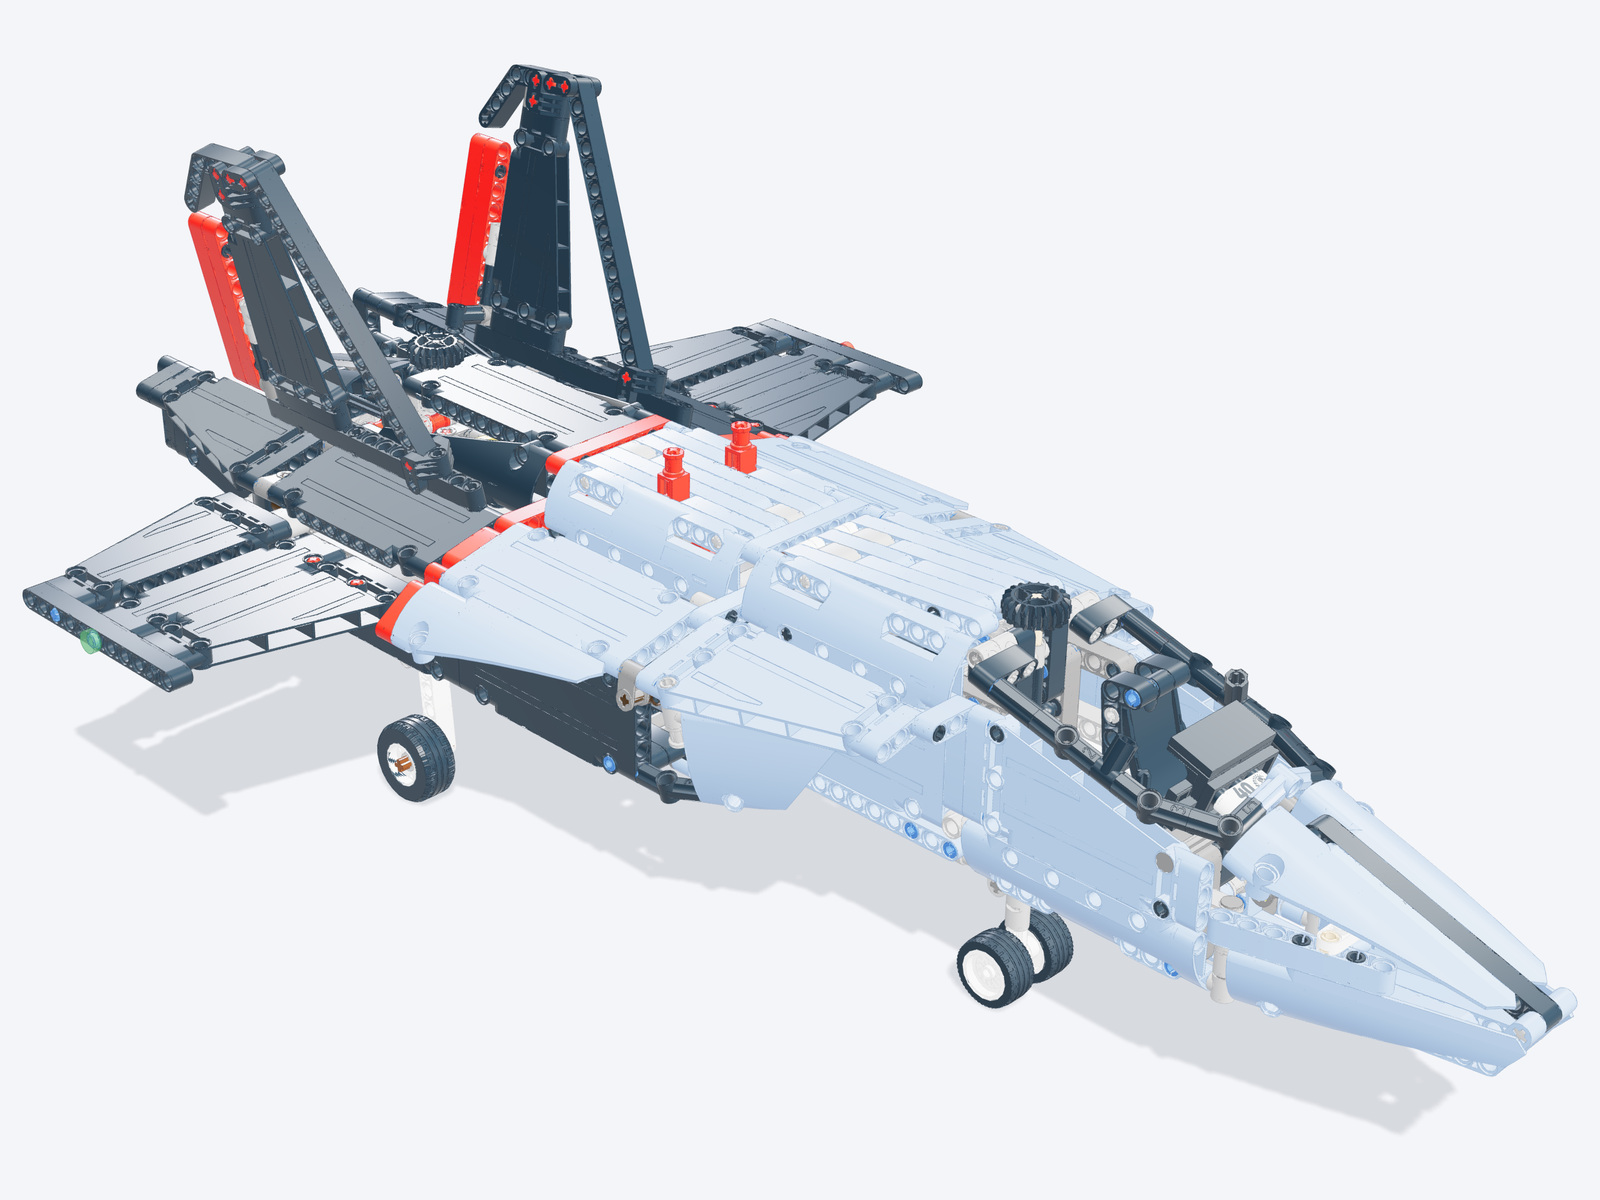
\includegraphics[width=.48\linewidth]{figures/ldraw/print/omr-42066-iso.jpg}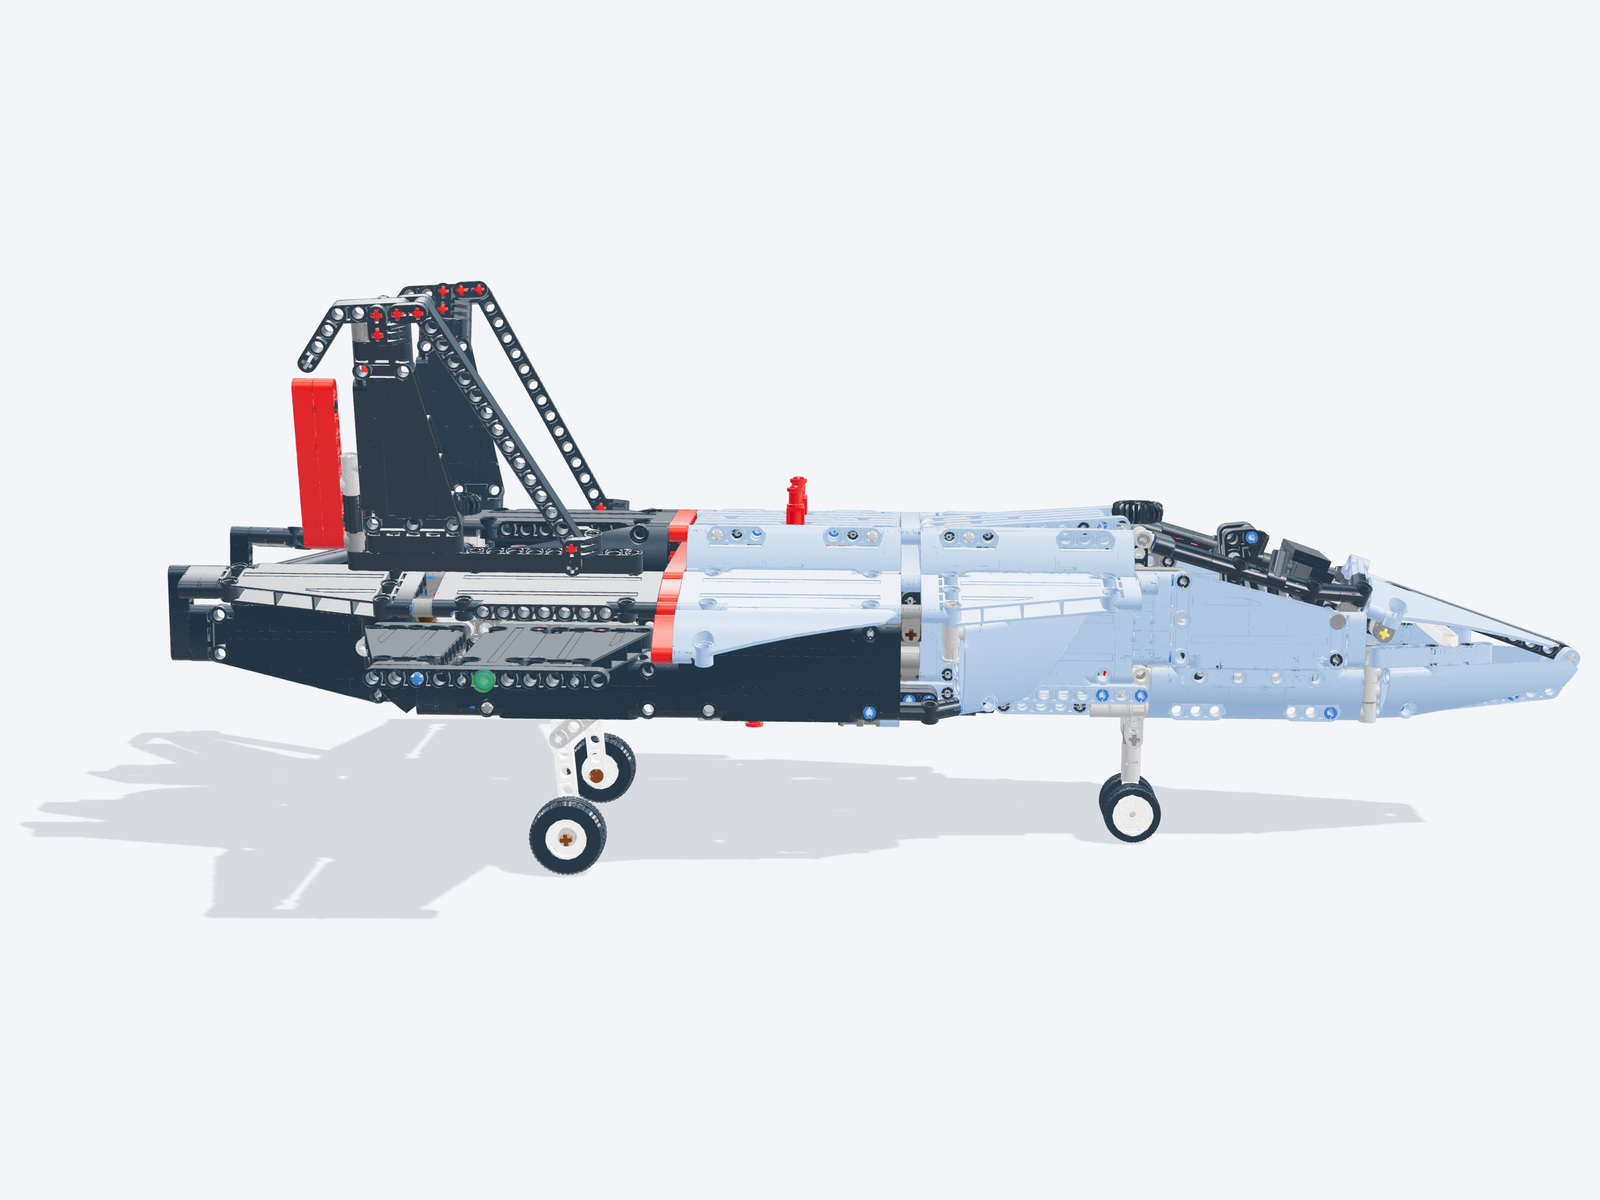
\includegraphics[width=.48\linewidth]{figures/ldraw/print/omr-42066-front.jpg}\\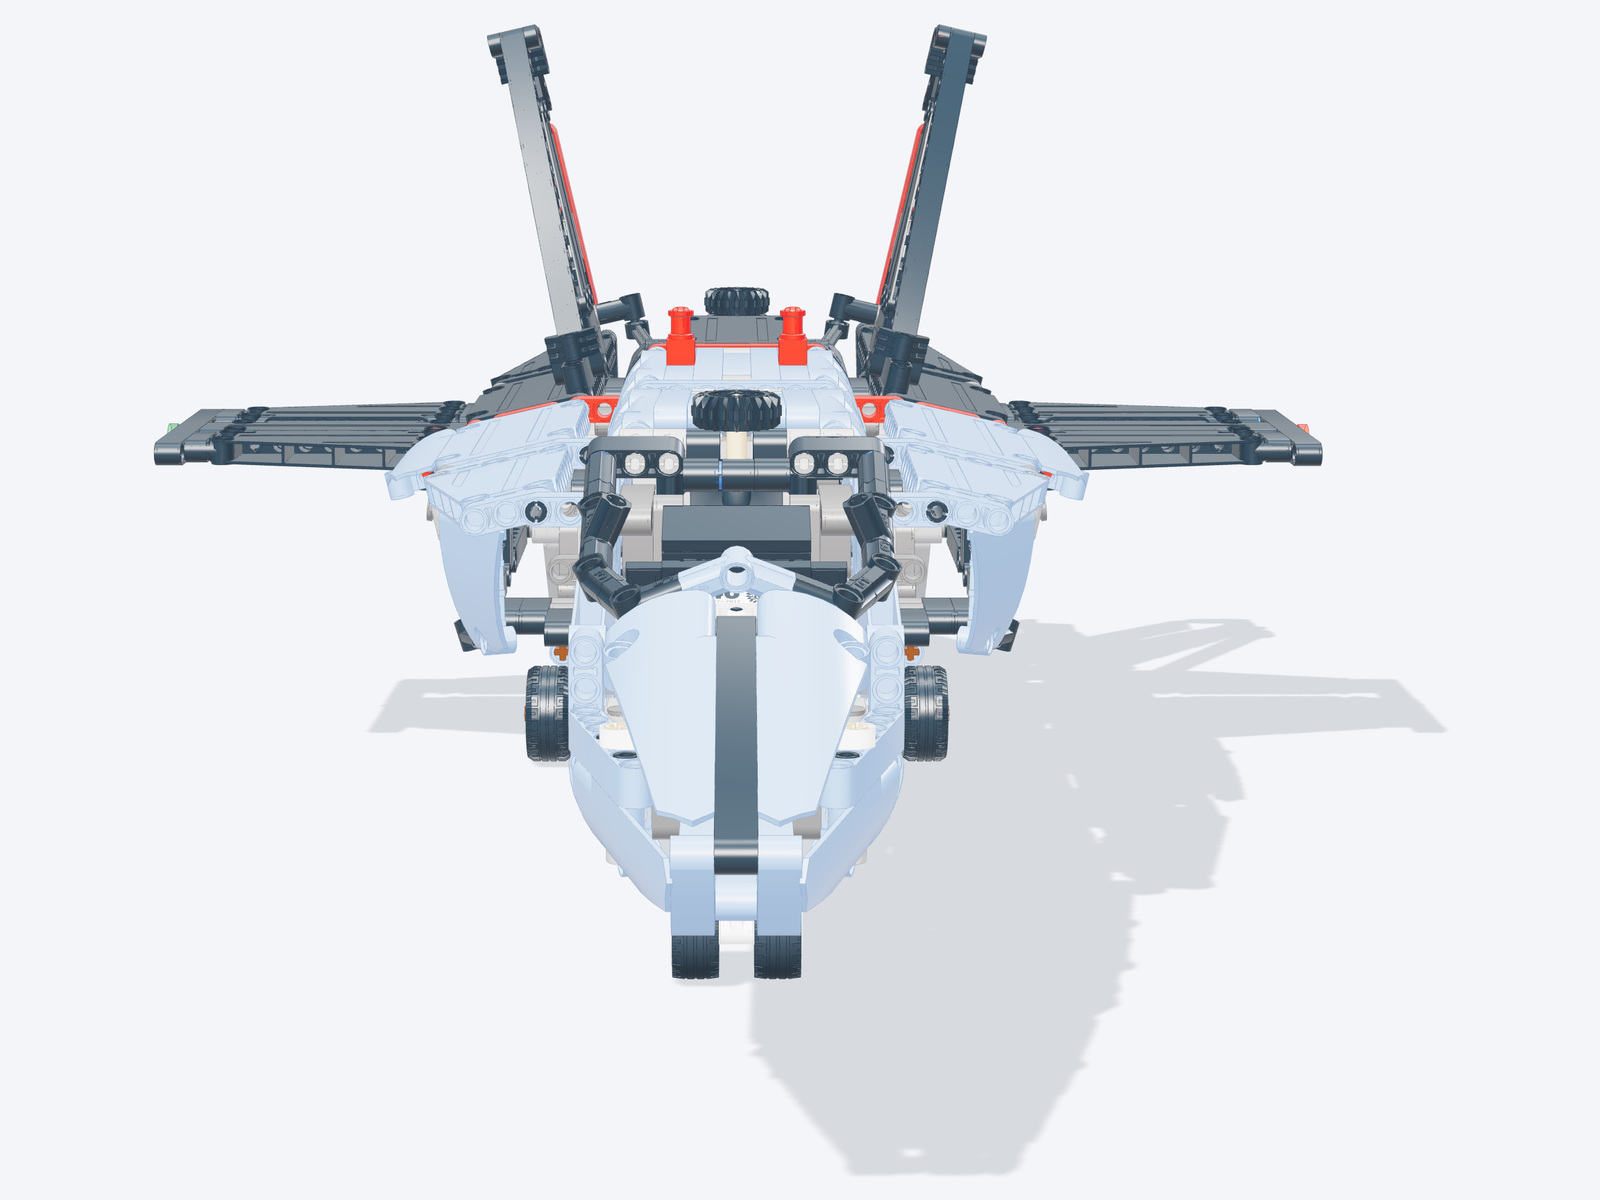
\includegraphics[width=.48\linewidth]{figures/ldraw/print/omr-42066-side.jpg}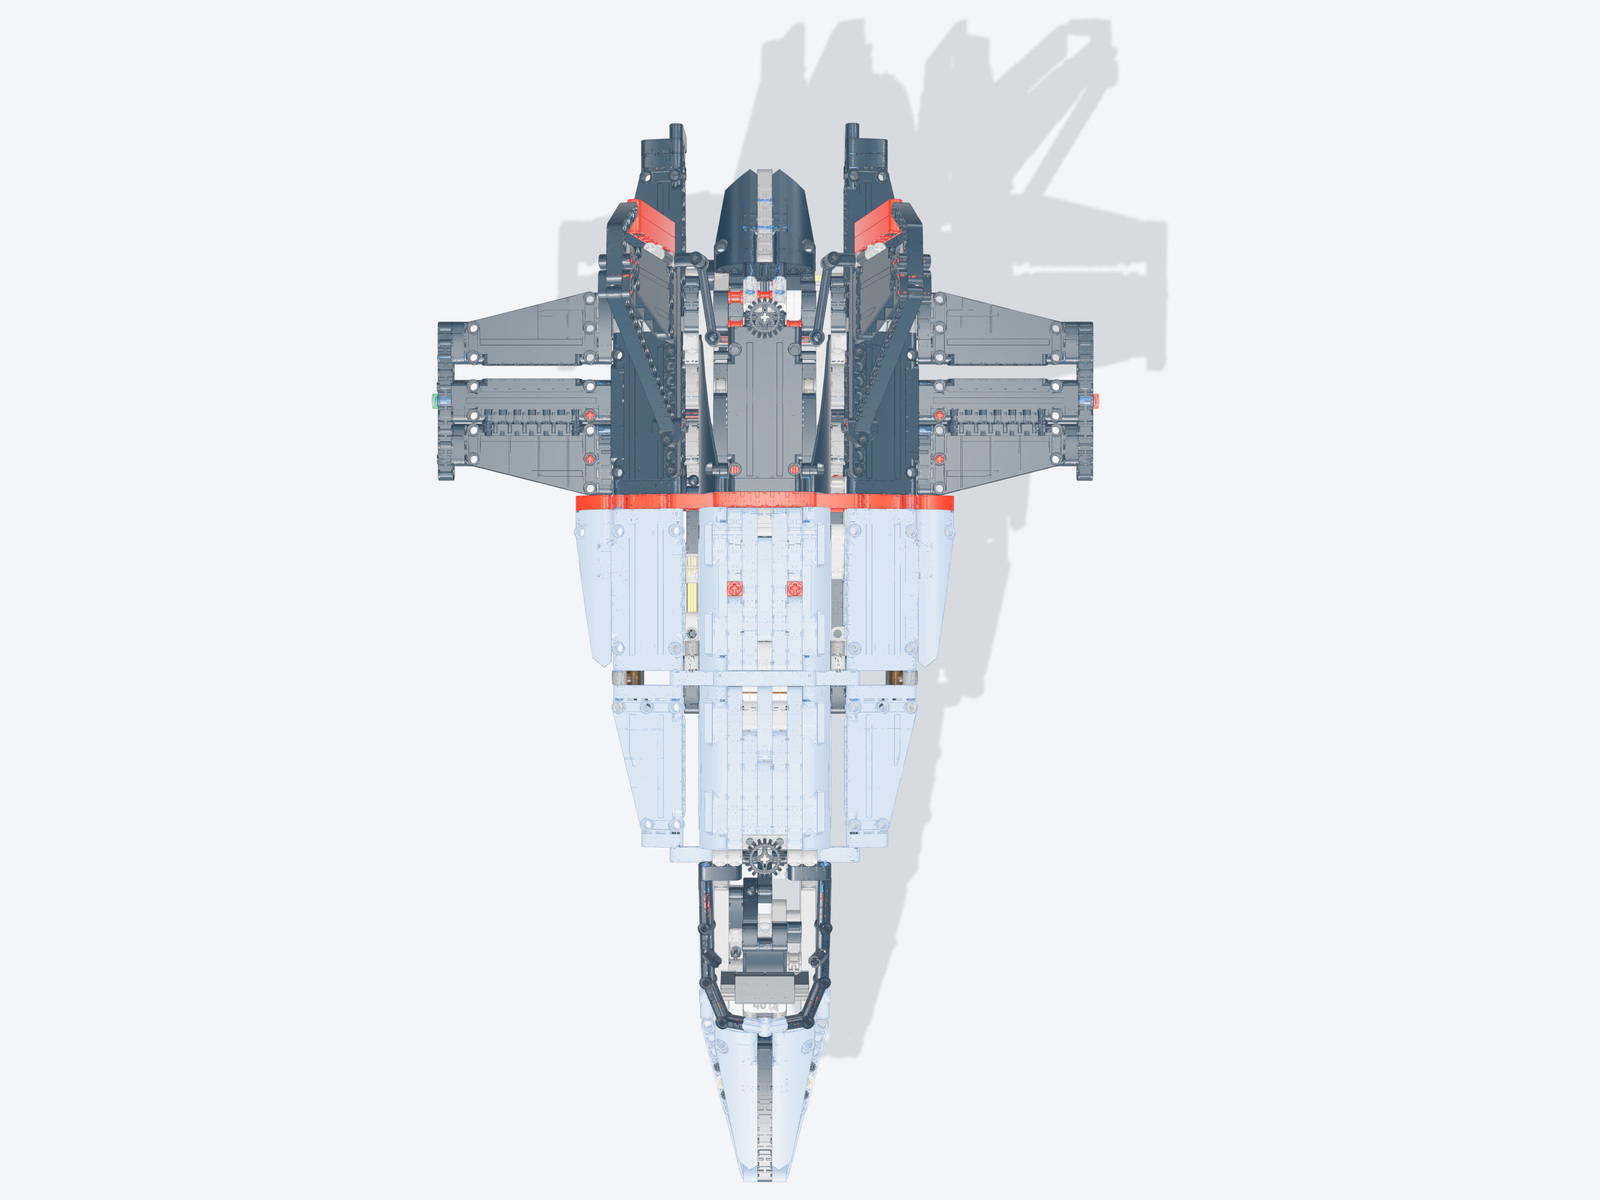
\includegraphics[width=.48\linewidth]{figures/ldraw/print/omr-42066-top.jpg}\end{center}
\paragraph{Attribution.}Philippe Hurbain [Philo]. CC BY 2.0.\par\noindent\url{https://library.ldraw.org/library/omr/42066-1.mpd}
\paragraph{Source lock.}\small\texttt{d1463b1464a83d54a6ed372fba732eab}\\\texttt{af79b3857185f4ab60b314e741caa067}\normalsize
\paragraph{Evidence coverage.}Connector definitions cover 90.84\% of instances. The audit reports 133 recognized-graph components and 90 intersection candidates without a recognized mating pair. 114 instances have no connector definition. These counts do not certify physical defects or gravitational stability.
\paragraph{Instructions.}141 expanded author steps.
\clearpage\subsection{Numbered visual input and complete question index}
Only relevant numbers are shown. The website can isolate any instance; public visual tasks provide their own numbered images. The following entries give every English prompt, all choice options, compact public evidence and the reference output. Raw repeated connector records and full action fact sets remain in the versioned JSON.
\begin{center}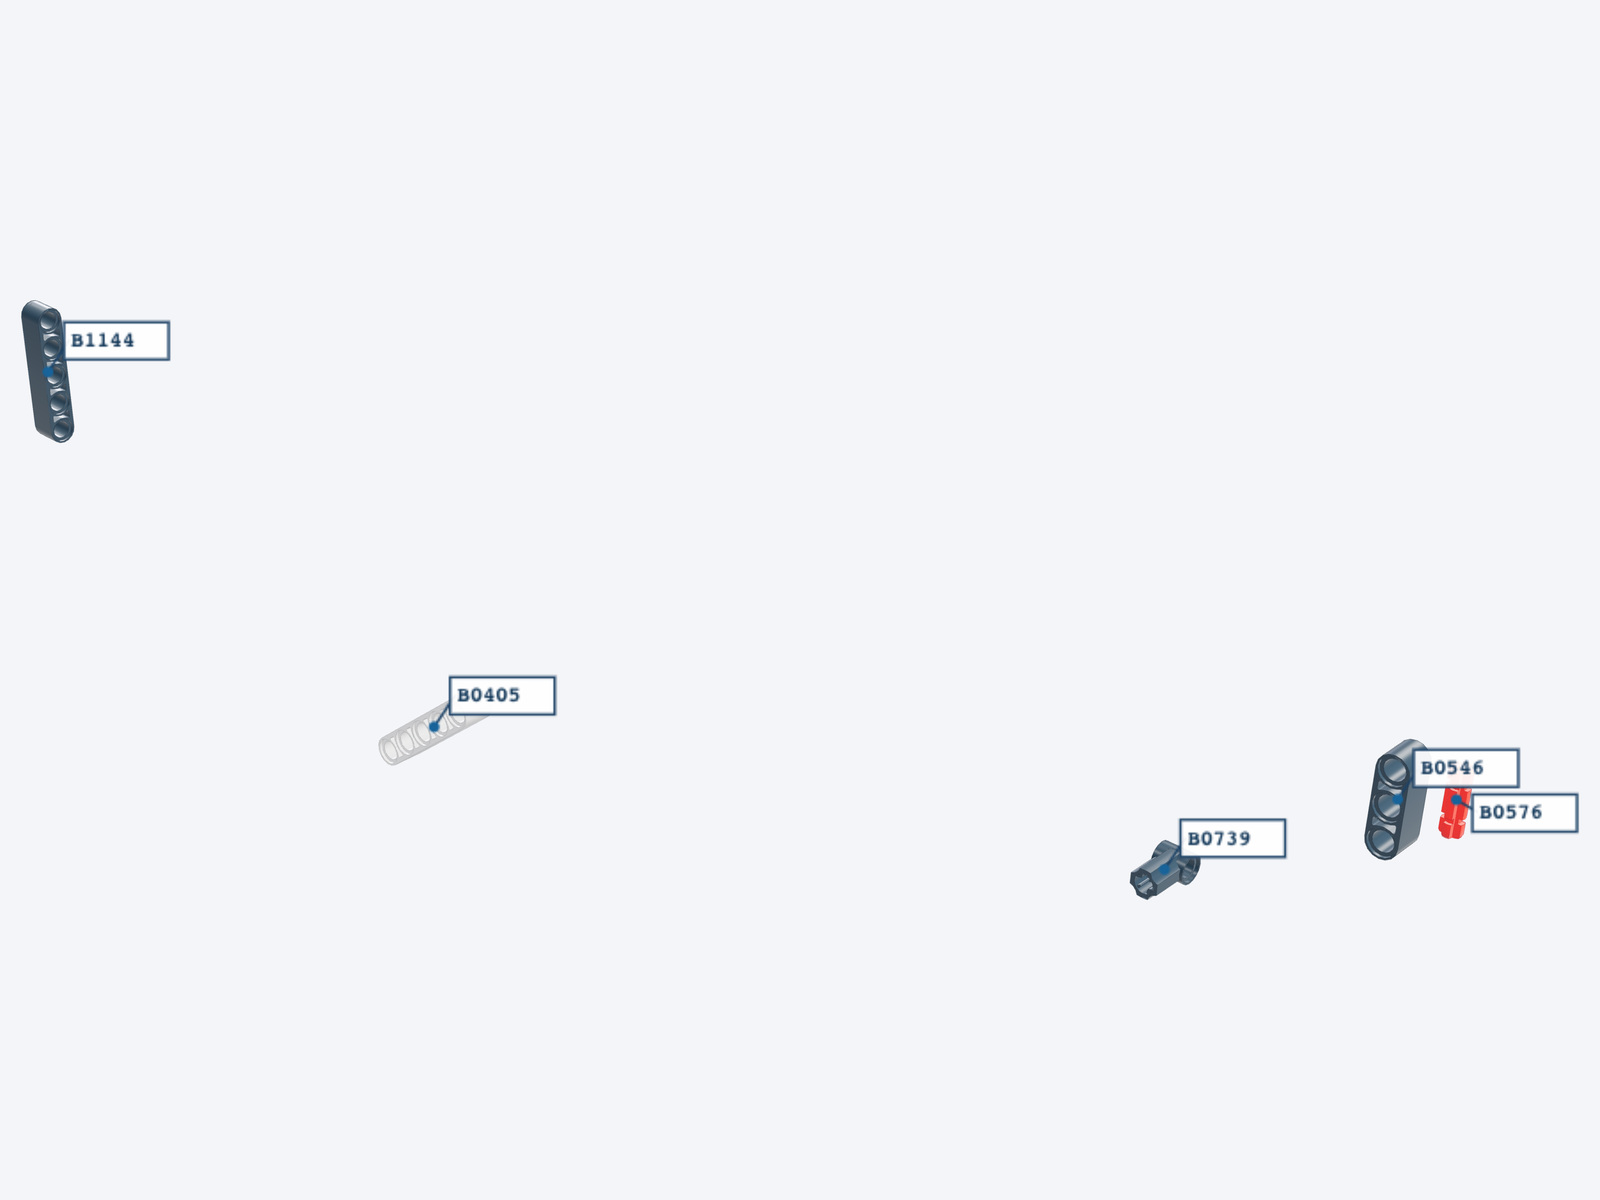
\includegraphics[width=.55\linewidth]{figures/ldraw/print/omr-42066-numbered.jpg}\end{center}
\begin{enumerate}
\item \textbf{color-1}. Identify the original color of B1144; numbered isolation is allowed.\par {\small \textit{Input:} Numbered visual input; source attributes are withheld from the model. \par\textit{Options:} A: Blue; B: Black; C: Yellow; D: White. \par\textit{Reference output:} B.}
\item \textbf{shape-match-1}. Ignoring color and pose, which numbered instance has the same LDraw part type as B1144?\par {\small \textit{Input:} Numbered visual input; source attributes are withheld from the model. \par\textit{Options:} A: B0546; B: B0405; C: B0739; D: B0576. \par\textit{Reference output:} B.}
\item \textbf{distance-1}. Using the supplied geometry bounding-box centers, which candidate is nearest to B1144?\par {\small \textit{Input:} Centers (mm): B1144 = (-47.588, 105.202992, -266.945856); B1226 = (58.8468, 166.972, -189.987204); B0947 = (0, 64.148442, 284.320131); B0240 = (20, 85.6348, 20.876756). \par\textit{Options:} A: B1226; B: B0240; C: B0947. \par\textit{Reference output:} A.}
\item \textbf{color-2}. Identify the original color of B0286; numbered isolation is allowed.\par {\small \textit{Input:} Numbered visual input; source attributes are withheld from the model. \par\textit{Options:} A: Black; B: Dark Brown; C: Trans Green; D: Trans Red. \par\textit{Reference output:} A.}
\item \textbf{shape-match-2}. Ignoring color and pose, which numbered instance has the same LDraw part type as B0286?\par {\small \textit{Input:} Numbered visual input; source attributes are withheld from the model. \par\textit{Options:} A: B0128; B: B0604; C: B0175; D: B0867. \par\textit{Reference output:} A.}
\item \textbf{distance-2}. Using the supplied geometry bounding-box centers, which candidate is nearest to B0286?\par {\small \textit{Input:} Centers (mm): B0286 = (-26, 101.822608, 2.184334); B0757 = (15.9892, 61.5388, 20.5948); B0964 = (15.800047, 98.829629, 261.097606); B0584 = (-16, 131.207349, 129.781993). \par\textit{Options:} A: B0584; B: B0964; C: B0757. \par\textit{Reference output:} C.}
\item \textbf{color-3}. Identify the original color of B0606; numbered isolation is allowed.\par {\small \textit{Input:} Numbered visual input; source attributes are withheld from the model. \par\textit{Options:} A: Yellow; B: Rubber Black; C: Dark Bluish Grey; D: Blue. \par\textit{Reference output:} D.}
\item \textbf{shape-match-3}. Ignoring color and pose, which numbered instance has the same LDraw part type as B0606?\par {\small \textit{Input:} Numbered visual input; source attributes are withheld from the model. \par\textit{Options:} A: B1082; B: B0435; C: B0302; D: B1052. \par\textit{Reference output:} A.}
\item \textbf{distance-3}. Using the supplied geometry bounding-box centers, which candidate is nearest to B0606?\par {\small \textit{Input:} Centers (mm): B0606 = (12.1, 106.503744, 166.636178); B1010 = (-31.6688, 124.275493, 152.61352); B0658 = (40, 85.5388, 28.8768); B1003 = (29.695036, 112.555599, 194.485323). \par\textit{Options:} A: B1003; B: B1010; C: B0658. \par\textit{Reference output:} A.}
\item \textbf{color-4}. Identify the original color of B0478; numbered isolation is allowed.\par {\small \textit{Input:} Numbered visual input; source attributes are withheld from the model. \par\textit{Options:} A: Blue; B: Tan; C: White; D: Light Bluish Grey. \par\textit{Reference output:} A.}
\item \textbf{shape-match-4}. Ignoring color and pose, which numbered instance has the same LDraw part type as B0478?\par {\small \textit{Input:} Numbered visual input; source attributes are withheld from the model. \par\textit{Options:} A: B0947; B: B0402; C: B1073; D: B0305. \par\textit{Reference output:} A.}
\item \textbf{distance-4}. Using the supplied geometry bounding-box centers, which candidate is nearest to B0478?\par {\small \textit{Input:} Centers (mm): B0478 = (16, 59.4268, 204.5888); B0569 = (28, 116.1948, 141.2608); B0379 = (-24, 110.8828, -82.8352); B0103 = (-29.50087, 89.069647, -28.56805). \par\textit{Options:} A: B0379; B: B0103; C: B0569. \par\textit{Reference output:} C.}
\item \textbf{color-5}. Identify the original color of B0644; numbered isolation is allowed.\par {\small \textit{Input:} Numbered visual input; source attributes are withheld from the model. \par\textit{Options:} A: Dark Brown; B: Light Bluish Grey; C: Medium Blue; D: Yellow. \par\textit{Reference output:} B.}
\item \textbf{shape-match-5}. Ignoring color and pose, which numbered instance has the same LDraw part type as B0644?\par {\small \textit{Input:} Numbered visual input; source attributes are withheld from the model. \par\textit{Options:} A: B0744; B: B0945; C: B0566; D: B0352. \par\textit{Reference output:} B.}
\item \textbf{distance-5}. Using the supplied geometry bounding-box centers, which candidate is nearest to B0644?\par {\small \textit{Input:} Centers (mm): B0644 = (24, 59.2348, 216.398877); B0306 = (-44.4, 79.183139, -81.276917); B1071 = (0.0008, 133.7308, 13.4528); B0074 = (-24, 68.845746, -90.005559). \par\textit{Options:} A: B0306; B: B0074; C: B1071. \par\textit{Reference output:} C.}
\item \textbf{interface-1}. Classify the supplied connector record for B0785 and B0786. This does not certify load capacity.\par {\small \textit{Input:} Record: family = axle; connector indices = 0, 0. \par\textit{Options:} A: ball; B: fixed; C: axle; D: hinge. \par\textit{Reference output:} C.}
\item \textbf{interface-2}. Classify the supplied connector record for B0692 and B0694. This does not certify load capacity.\par {\small \textit{Input:} Record: family = ball; connector indices = 1, 0. \par\textit{Options:} A: ball; B: axle; C: fixed; D: hinge. \par\textit{Reference output:} A.}
\item \textbf{interface-3}. Classify the supplied connector record for B0413 and B0414. This does not certify load capacity.\par {\small \textit{Input:} Record: family = fixed; connector indices = 1, 1. \par\textit{Options:} A: fixed; B: hinge; C: ball; D: axle. \par\textit{Reference output:} A.}
\item \textbf{interface-4}. Classify the supplied connector record for B0553 and B0551. This does not certify load capacity.\par {\small \textit{Input:} Record: family = hinge; connector indices = 0, 1. \par\textit{Options:} A: axle; B: ball; C: hinge; D: fixed. \par\textit{Reference output:} C.}
\item \textbf{interface-5}. Classify the supplied connector record for B0988 and B0994. This does not certify load capacity.\par {\small \textit{Input:} Record: family = stud; connector indices = 8, 2. \par\textit{Options:} A: ball; B: hinge; C: stud; D: fixed; E: axle. \par\textit{Reference output:} C.}
\item \textbf{neighbors-1}. Select every candidate directly adjacent to B1156 in the supplied connector graph.\par {\small \textit{Input:} Unique undirected pairs: B1145 / B1156; B1156 / B1157. \par\textit{Options:} A: B1157; B: B1123; C: B0368; D: B1145. \par\textit{Reference output:} A, D.}
\item \textbf{graph-removal-1}. Delete B1156 and its incident edges from this local graph. How many connected components remain? Do not infer physical extractability.\par {\small \textit{Input:} Nodes: B1156, B1157, B1145, B0368, B1123. Unique undirected pairs: B1145 / B1156; B1156 / B1157. \par\textit{Options:} A: 5; B: 4; C: 3; D: 6. \par\textit{Reference output:} B.}
\item \textbf{neighbors-2}. Select every candidate directly adjacent to B0916 in the supplied connector graph.\par {\small \textit{Input:} Unique undirected pairs: B0426 / B0916; B0915 / B0916. \par\textit{Options:} A: B0824; B: B0426; C: B0176; D: B0915. \par\textit{Reference output:} B, D.}
\item \textbf{graph-removal-2}. Delete B0916 and its incident edges from this local graph. How many connected components remain? Do not infer physical extractability.\par {\small \textit{Input:} Nodes: B0916, B0426, B0915, B0176, B0824. Unique undirected pairs: B0426 / B0916; B0915 / B0916. \par\textit{Options:} A: 6; B: 3; C: 4; D: 5. \par\textit{Reference output:} C.}
\item \textbf{neighbors-3}. Select every candidate directly adjacent to B1244 in the supplied connector graph.\par {\small \textit{Input:} Unique undirected pairs: B1242 / B1244; B1243 / B1244. \par\textit{Options:} A: B1242; B: B0013; C: B0583; D: B1243. \par\textit{Reference output:} A, D.}
\item \textbf{graph-removal-3}. Delete B1244 and its incident edges from this local graph. How many connected components remain? Do not infer physical extractability.\par {\small \textit{Input:} Nodes: B1244, B1243, B1242, B0583, B0013. Unique undirected pairs: B1242 / B1244; B1243 / B1244. \par\textit{Options:} A: 3; B: 6; C: 5; D: 4. \par\textit{Reference output:} D.}
\item \textbf{neighbors-4}. Select every candidate directly adjacent to B0962 in the supplied connector graph.\par {\small \textit{Input:} Unique undirected pairs: B0960 / B0962; B0961 / B0962. \par\textit{Options:} A: B1087; B: B0960; C: B0847; D: B0961. \par\textit{Reference output:} B, D.}
\item \textbf{graph-removal-4}. Delete B0962 and its incident edges from this local graph. How many connected components remain? Do not infer physical extractability.\par {\small \textit{Input:} Nodes: B0962, B0960, B0961, B0847, B1087. Unique undirected pairs: B0960 / B0962; B0961 / B0962. \par\textit{Options:} A: 5; B: 6; C: 4; D: 3. \par\textit{Reference output:} C.}
\item \textbf{neighbors-5}. Select every candidate directly adjacent to B1003 in the supplied connector graph.\par {\small \textit{Input:} Unique undirected pairs: B1001 / B1003; B1003 / B1005. \par\textit{Options:} A: B0769; B: B1001; C: B0741; D: B1005. \par\textit{Reference output:} B, D.}
\item \textbf{graph-removal-5}. Delete B1003 and its incident edges from this local graph. How many connected components remain? Do not infer physical extractability.\par {\small \textit{Input:} Nodes: B1003, B1001, B1005, B0741, B0769. Unique undirected pairs: B1001 / B1003; B1003 / B1005. \par\textit{Options:} A: 3; B: 4; C: 6; D: 5. \par\textit{Reference output:} B.}
\item \textbf{coverage-1}. Which numbered instance lacks a connector definition in the coverage record, so this audit cannot establish that it is floating?\par {\small \textit{Input:} Definition coverage: B0025 = unsupported; B1144 = supported; B0286 = supported; B0606 = supported. \par\textit{Options:} A: B0606; B: B0025; C: B0286; D: B1144. \par\textit{Reference output:} B.}
\item \textbf{evidence-limit-1}. Only source geometry, connector matching and mesh intersection audits are available. Without mass, friction, material or dynamic tests, is gravitational stability established?\par {\small \textit{Input:} Available evidence: Original CAD; Connector inference; Inset-mesh intersection candidates. \par\textit{Options:} A: Established; B: Not established by this evidence. \par\textit{Reference output:} B.}
\item \textbf{source-step-1}. At which expanded author step does B0163 first appear in the supplied source-step table? Source order is not a collision-free assembly proof.\par {\small \textit{Input:} Expanded author records: step 1: B0001; step 13: B0163. \par\textit{Options:} A: 15; B: 14; C: 12; D: 13. \par\textit{Reference output:} D.}
\item \textbf{source-step-2}. At which expanded author step does B0709 first appear in the supplied source-step table? Source order is not a collision-free assembly proof.\par {\small \textit{Input:} Expanded author records: step 1: B0001; step 73: B0709. \par\textit{Options:} A: 75; B: 72; C: 74; D: 73. \par\textit{Reference output:} D.}
\item \textbf{source-step-3}. At which expanded author step does B0804 first appear in the supplied source-step table? Source order is not a collision-free assembly proof.\par {\small \textit{Input:} Expanded author records: step 1: B0001; step 84: B0804. \par\textit{Options:} A: 85; B: 86; C: 84; D: 83. \par\textit{Reference output:} C.}
\item \textbf{source-step-4}. At which expanded author step does B1237 first appear in the supplied source-step table? Source order is not a collision-free assembly proof.\par {\small \textit{Input:} Expanded author records: step 1: B0001; step 141: B1237. \par\textit{Options:} A: 142; B: 140; C: 141; D: 143. \par\textit{Reference output:} C.}
\item \textbf{source-step-5}. At which expanded author step does B1173 first appear in the supplied source-step table? Source order is not a collision-free assembly proof.\par {\small \textit{Input:} Expanded author records: step 1: B0001; step 133: B1173. \par\textit{Options:} A: 135; B: 132; C: 133; D: 134. \par\textit{Reference output:} C.}
\item \textbf{source-sequence-1}. Reveal the supplied source-step window in author order. Actions change visibility only, without simulating insertion trajectories.\par {\small \textit{Input:} Source window: step-1: B0001, B0002, B0003, B0004, B0005, B0006; step-2: B0007, B0008, B0009, B0010, B0011, B0012, B0013; step-3: B0014, B0015, B0016, B0017, B0018, B0019, B0020, B0021; step-4: B0022; step-5: B0023, B0024; step-6: B0025, B0026, B0027, B0028, B0029, B0030, B0031, B0032, B0033, B0034, B0035, B0036, B0037, B0038, B0039, B0040, B0041, B0042, B0043, B0044, B0045, B0046, B0047, B0048, B0049, B0050, B0051, B0052, B0053, B0054, B0055, B0056, B0057, B0058, B0059, B0060, B0061, B0062, B0063, B0064, B0065, B0066, B0067, B0068, B0069, B0070, B0071, B0072, B0073, B0074, B0075, B0076, B0077, B0078, B0079, B0080, B0081, B0082, B0083, B0084, B0085, B0086, B0087, B0088, B0089, B0090, B0091, B0092, B0093, B0094, B0095, B0096, B0097, B0098, B0099, B0100, B0101, B0102, B0103, B0104, B0105, B0106, B0107, B0108, B0109, B0110, B0111, B0112, B0113, B0114, B0115, B0116, B0117, B0118, B0119, B0120, B0121. Action budget: 6. \par\textit{Reference output:} step-1, step-2, step-3, step-4, step-5, step-6.}
\item \textbf{restore-instance-1}. The display copy hides B1144. Restore only that numbered instance, preserving all other instances and source poses.\par {\small \textit{Input:} Target: B1144. Action budget: 1. All other instances initially remain visible. \par\textit{Reference output:} restore-B1144.}
\item \textbf{restore-instance-2}. The display copy hides B0286. Restore only that numbered instance, preserving all other instances and source poses.\par {\small \textit{Input:} Target: B0286. Action budget: 1. All other instances initially remain visible. \par\textit{Reference output:} restore-B0286.}
\item \textbf{restore-instance-3}. The display copy hides B0606. Restore only that numbered instance, preserving all other instances and source poses.\par {\small \textit{Input:} Target: B0606. Action budget: 1. All other instances initially remain visible. \par\textit{Reference output:} restore-B0606.}
\end{enumerate}
\clearpage
\section{10213: Shuttle Adventure}
1254 source instances; 34 tasks; D4 scale band.

\par\noindent Perspective, front, side and top views follow in reading order. Original source transforms are preserved.
\begin{center}
\includegraphics[width=.48\linewidth]{figures/ldraw/print/10213-iso.jpg}
\includegraphics[width=.48\linewidth]{figures/ldraw/print/10213-front.jpg}\\
\includegraphics[width=.48\linewidth]{figures/ldraw/print/10213-side.jpg}
\includegraphics[width=.48\linewidth]{figures/ldraw/print/10213-top.jpg}\end{center}
\paragraph{Attribution.}Edward Carman [EdmanZA]. CC BY 2.0.\par\noindent\url{https://library.ldraw.org/omr/sets/870}
\paragraph{Source lock.}\small\texttt{e295434c8fc8c067e6cd01c398dccd30}\\\texttt{59a38799f03a6cecddb9319ecf16d909}\normalsize
\paragraph{Evidence coverage.}Connector definitions cover 99.36\% of instances. The audit reports 25 recognized-graph components and 63 intersection candidates without a recognized mating pair. 8 instances have no connector definition. These counts do not certify physical defects or gravitational stability.
\paragraph{Instructions.}No author STEP replay or source-order question is provided.
\clearpage\subsection{Numbered visual input and complete question index}
Only relevant numbers are shown. The website can isolate any instance; public visual tasks provide their own numbered images. The following entries give every English prompt, all choice options, compact public evidence and the reference output. Raw repeated connector records and full action fact sets remain in the versioned JSON.
\begin{center}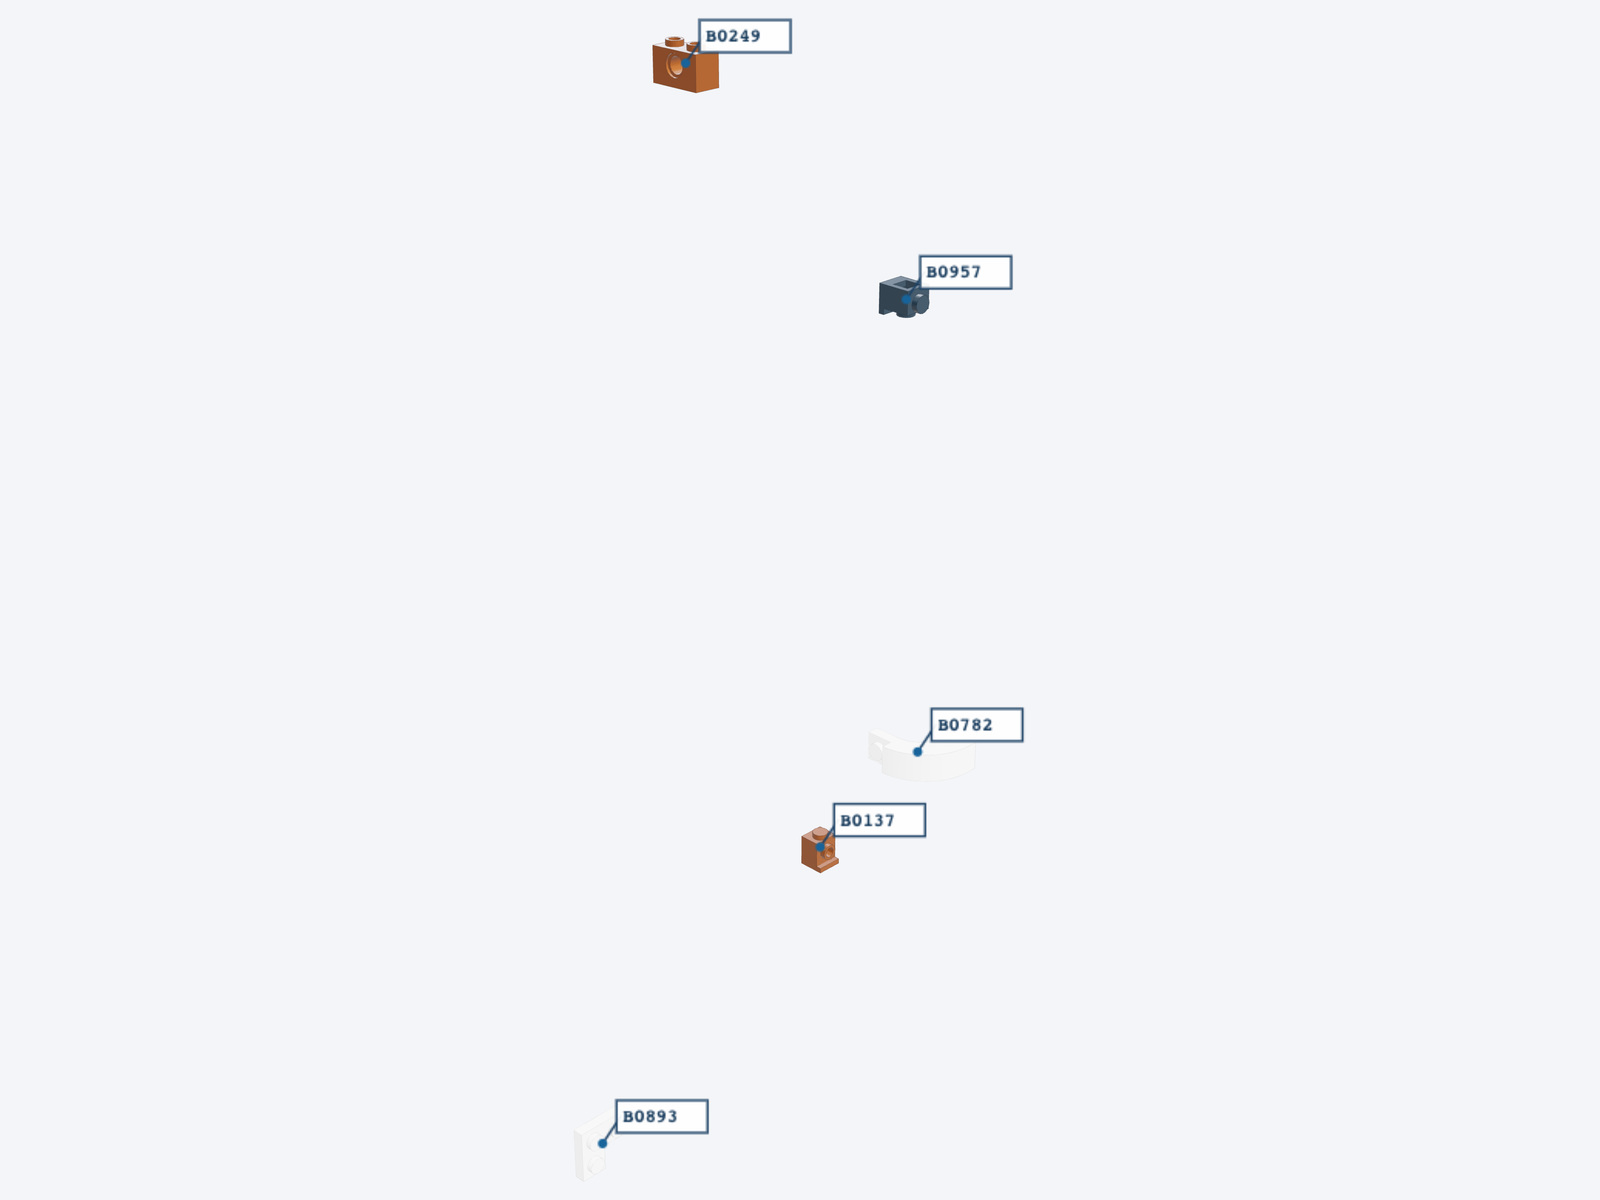
\includegraphics[width=.55\linewidth]{figures/ldraw/print/10213-numbered.jpg}\end{center}
\begin{enumerate}
\item \textbf{color-1}. Identify the original color of B0957; numbered isolation is allowed.\par {\small \textit{Input:} Numbered visual input; source attributes are withheld from the model. \par\textit{Options:} A: White; B: Dark Blue; C: Black; D: Trans Brown. \par\textit{Reference output:} C.}
\item \textbf{shape-match-1}. Ignoring color and pose, which numbered instance has the same LDraw part type as B0957?\par {\small \textit{Input:} Numbered visual input; source attributes are withheld from the model. \par\textit{Options:} A: B0893; B: B0137; C: B0249; D: B0782. \par\textit{Reference output:} B.}
\item \textbf{distance-1}. Using the supplied geometry bounding-box centers, which candidate is nearest to B0957?\par {\small \textit{Input:} Centers (mm): B0957 = (-4, 297.6, 23.2); B0713 = (-16.1, 237.6, 7.2); B0706 = (0, 113.452, 13.3412); B0762 = (-20, 237.6, 21.6). \par\textit{Options:} A: B0706; B: B0713; C: B0762. \par\textit{Reference output:} C.}
\item \textbf{color-2}. Identify the original color of B0396; numbered isolation is allowed.\par {\small \textit{Input:} Numbered visual input; source attributes are withheld from the model. \par\textit{Options:} A: Dark Bluish Grey; B: Dark Blue; C: Light Bluish Grey; D: Reddish Brown. \par\textit{Reference output:} A.}
\item \textbf{shape-match-2}. Ignoring color and pose, which numbered instance has the same LDraw part type as B0396?\par {\small \textit{Input:} Numbered visual input; source attributes are withheld from the model. \par\textit{Options:} A: B0469; B: B0388; C: B1086; D: B0268. \par\textit{Reference output:} B.}
\item \textbf{distance-2}. Using the supplied geometry bounding-box centers, which candidate is nearest to B0396?\par {\small \textit{Input:} Centers (mm): B0396 = (36, 325.6, -34.4); B0394 = (36, 277.6, -34.4); B0106 = (130.111595, 62.1388, -141.423595); B1116 = (-21.0432, 41.9484, 41.6). \par\textit{Options:} A: B1116; B: B0394; C: B0106. \par\textit{Reference output:} B.}
\item \textbf{color-3}. Identify the original color of B0228; numbered isolation is allowed.\par {\small \textit{Input:} Numbered visual input; source attributes are withheld from the model. \par\textit{Options:} A: Dark Brown; B: Tan; C: Reddish Brown; D: Trans Clear. \par\textit{Reference output:} C.}
\item \textbf{shape-match-3}. Ignoring color and pose, which numbered instance has the same LDraw part type as B0228?\par {\small \textit{Input:} Numbered visual input; source attributes are withheld from the model. \par\textit{Options:} A: B0303; B: B0921; C: B0237; D: B1084. \par\textit{Reference output:} A.}
\item \textbf{distance-3}. Using the supplied geometry bounding-box centers, which candidate is nearest to B0228?\par {\small \textit{Input:} Centers (mm): B0228 = (0, 266.4, -40); B0150 = (-12, 109.6, -15.2); B0732 = (0, 69.7, 23.2); B1155 = (4, 209.6, 15.2). \par\textit{Options:} A: B0732; B: B0150; C: B1155. \par\textit{Reference output:} C.}
\item \textbf{color-4}. Identify the original color of B0987; numbered isolation is allowed.\par {\small \textit{Input:} Numbered visual input; source attributes are withheld from the model. \par\textit{Options:} A: Metallic Gold; B: Trans Clear; C: Blue; D: White. \par\textit{Reference output:} D.}
\item \textbf{shape-match-4}. Ignoring color and pose, which numbered instance has the same LDraw part type as B0987?\par {\small \textit{Input:} Numbered visual input; source attributes are withheld from the model. \par\textit{Options:} A: B0580; B: B0348; C: B0260; D: B0189. \par\textit{Reference output:} B.}
\item \textbf{distance-4}. Using the supplied geometry bounding-box centers, which candidate is nearest to B0987?\par {\small \textit{Input:} Centers (mm): B0987 = (-12, 117.6, 16); B0588 = (44, 109.6, -2.4); B0146 = (-24.8, 109.6, -52); B0260 = (20, 349.6, -20). \par\textit{Options:} A: B0588; B: B0146; C: B0260. \par\textit{Reference output:} A.}
\item \textbf{color-5}. Identify the original color of B0984; numbered isolation is allowed.\par {\small \textit{Input:} Numbered visual input; source attributes are withheld from the model. \par\textit{Options:} A: Black; B: Metallic Gold; C: Yellow; D: Trans Red. \par\textit{Reference output:} A.}
\item \textbf{shape-match-5}. Ignoring color and pose, which numbered instance has the same LDraw part type as B0984?\par {\small \textit{Input:} Numbered visual input; source attributes are withheld from the model. \par\textit{Options:} A: B1072; B: B0926; C: B0881; D: B0356. \par\textit{Reference output:} B.}
\item \textbf{distance-5}. Using the supplied geometry bounding-box centers, which candidate is nearest to B0984?\par {\small \textit{Input:} Centers (mm): B0984 = (-20, 301.6, 4); B1060 = (-20, 300, 22.4); B0273 = (20, 349.6, -28); B1233 = (-30.6, 5.8, 170.8). \par\textit{Options:} A: B1233; B: B0273; C: B1060. \par\textit{Reference output:} C.}
\item \textbf{interface-1}. Classify the supplied connector record for B0645 and B0800. This does not certify load capacity.\par {\small \textit{Input:} Record: family = axle; connector indices = 1, 0. \par\textit{Options:} A: ball; B: axle; C: fixed; D: hinge. \par\textit{Reference output:} B.}
\item \textbf{interface-2}. Classify the supplied connector record for B0723 and B0724. This does not certify load capacity.\par {\small \textit{Input:} Record: family = fixed; connector indices = 1, 0. \par\textit{Options:} A: hinge; B: fixed; C: axle; D: ball. \par\textit{Reference output:} B.}
\item \textbf{interface-3}. Classify the supplied connector record for B1248 and B1244. This does not certify load capacity.\par {\small \textit{Input:} Record: family = hinge; connector indices = 0, 5. \par\textit{Options:} A: ball; B: fixed; C: hinge; D: axle. \par\textit{Reference output:} C.}
\item \textbf{interface-4}. Classify the supplied connector record for B0375 and B0391. This does not certify load capacity.\par {\small \textit{Input:} Record: family = stud; connector indices = 68, 9. \par\textit{Options:} A: fixed; B: hinge; C: stud; D: axle; E: ball. \par\textit{Reference output:} C.}
\item \textbf{neighbors-1}. Select every candidate directly adjacent to B0219 in the supplied connector graph.\par {\small \textit{Input:} Unique undirected pairs: B0178 / B0219; B0181 / B0219; B0187 / B0219; B0191 / B0219; B0196 / B0219; B0219 / B0224. \par\textit{Options:} A: B0178; B: B0984; C: B0224; D: B0191; E: B0446; F: B0181; G: B0187; H: B0196. \par\textit{Reference output:} A, C, D, F, G, H.}
\item \textbf{graph-removal-1}. Delete B0219 and its incident edges from this local graph. How many connected components remain? Do not infer physical extractability.\par {\small \textit{Input:} Nodes: B0219, B0224, B0181, B0187, B0196, B0191, B0178, B0984, B0446. Unique undirected pairs: B0178 / B0219; B0181 / B0219; B0187 / B0219; B0191 / B0219; B0196 / B0219; B0219 / B0224. \par\textit{Options:} A: 8; B: 10; C: 7; D: 9. \par\textit{Reference output:} A.}
\item \textbf{neighbors-2}. Select every candidate directly adjacent to B0487 in the supplied connector graph.\par {\small \textit{Input:} Unique undirected pairs: B0476 / B0487; B0487 / B0488. \par\textit{Options:} A: B0488; B: B1002; C: B0310; D: B0476. \par\textit{Reference output:} A, D.}
\item \textbf{graph-removal-2}. Delete B0487 and its incident edges from this local graph. How many connected components remain? Do not infer physical extractability.\par {\small \textit{Input:} Nodes: B0487, B0488, B0476, B1002, B0310. Unique undirected pairs: B0476 / B0487; B0487 / B0488. \par\textit{Options:} A: 3; B: 5; C: 4; D: 6. \par\textit{Reference output:} C.}
\item \textbf{neighbors-3}. Select every candidate directly adjacent to B0445 in the supplied connector graph.\par {\small \textit{Input:} Unique undirected pairs: B0440 / B0445; B0445 / B0449. \par\textit{Options:} A: B0570; B: B0601; C: B0440; D: B0449. \par\textit{Reference output:} C, D.}
\item \textbf{graph-removal-3}. Delete B0445 and its incident edges from this local graph. How many connected components remain? Do not infer physical extractability.\par {\small \textit{Input:} Nodes: B0445, B0449, B0440, B0601, B0570. Unique undirected pairs: B0440 / B0445; B0445 / B0449. \par\textit{Options:} A: 3; B: 5; C: 6; D: 4. \par\textit{Reference output:} D.}
\item \textbf{neighbors-4}. Select every candidate directly adjacent to B0668 in the supplied connector graph.\par {\small \textit{Input:} Unique undirected pairs: B0668 / B0669; B0668 / B0672. \par\textit{Options:} A: B0759; B: B0418; C: B0672; D: B0669. \par\textit{Reference output:} C, D.}
\item \textbf{graph-removal-4}. Delete B0668 and its incident edges from this local graph. How many connected components remain? Do not infer physical extractability.\par {\small \textit{Input:} Nodes: B0668, B0672, B0669, B0759, B0418. Unique undirected pairs: B0668 / B0669; B0668 / B0672. \par\textit{Options:} A: 3; B: 6; C: 4; D: 5. \par\textit{Reference output:} C.}
\item \textbf{neighbors-5}. Select every candidate directly adjacent to B0007 in the supplied connector graph.\par {\small \textit{Input:} Unique undirected pairs: B0001 / B0007; B0007 / B0023; B0007 / B0025. \par\textit{Options:} A: B0001; B: B0023; C: B1163; D: B0025; E: B0946. \par\textit{Reference output:} A, B, D.}
\item \textbf{graph-removal-5}. Delete B0007 and its incident edges from this local graph. How many connected components remain? Do not infer physical extractability.\par {\small \textit{Input:} Nodes: B0007, B0023, B0001, B0025, B0946, B1163. Unique undirected pairs: B0001 / B0007; B0007 / B0023; B0007 / B0025. \par\textit{Options:} A: 6; B: 4; C: 7; D: 5. \par\textit{Reference output:} D.}
\item \textbf{coverage-1}. Which numbered instance lacks a connector definition in the coverage record, so this audit cannot establish that it is floating?\par {\small \textit{Input:} Definition coverage: B0706 = unsupported; B0957 = supported; B0396 = supported; B0228 = supported. \par\textit{Options:} A: B0957; B: B0396; C: B0228; D: B0706. \par\textit{Reference output:} D.}
\item \textbf{evidence-limit-1}. Only source geometry, connector matching and mesh intersection audits are available. Without mass, friction, material or dynamic tests, is gravitational stability established?\par {\small \textit{Input:} Available evidence: Original CAD; Connector inference; Inset-mesh intersection candidates. \par\textit{Options:} A: Not established by this evidence; B: Established. \par\textit{Reference output:} A.}
\item \textbf{restore-instance-1}. The display copy hides B0957. Restore only that numbered instance, preserving all other instances and source poses.\par {\small \textit{Input:} Target: B0957. Action budget: 1. All other instances initially remain visible. \par\textit{Reference output:} restore-B0957.}
\item \textbf{restore-instance-2}. The display copy hides B0396. Restore only that numbered instance, preserving all other instances and source poses.\par {\small \textit{Input:} Target: B0396. Action budget: 1. All other instances initially remain visible. \par\textit{Reference output:} restore-B0396.}
\item \textbf{restore-instance-3}. The display copy hides B0228. Restore only that numbered instance, preserving all other instances and source poses.\par {\small \textit{Input:} Target: B0228. Action budget: 1. All other instances initially remain visible. \par\textit{Reference output:} restore-B0228.}
\end{enumerate}
\clearpage
\section{10265: Ford Mustang}
1357 source instances; 40 tasks; D4 scale band.

\par\noindent Perspective, front, side and top views follow in reading order. Original source transforms are preserved.
\begin{center}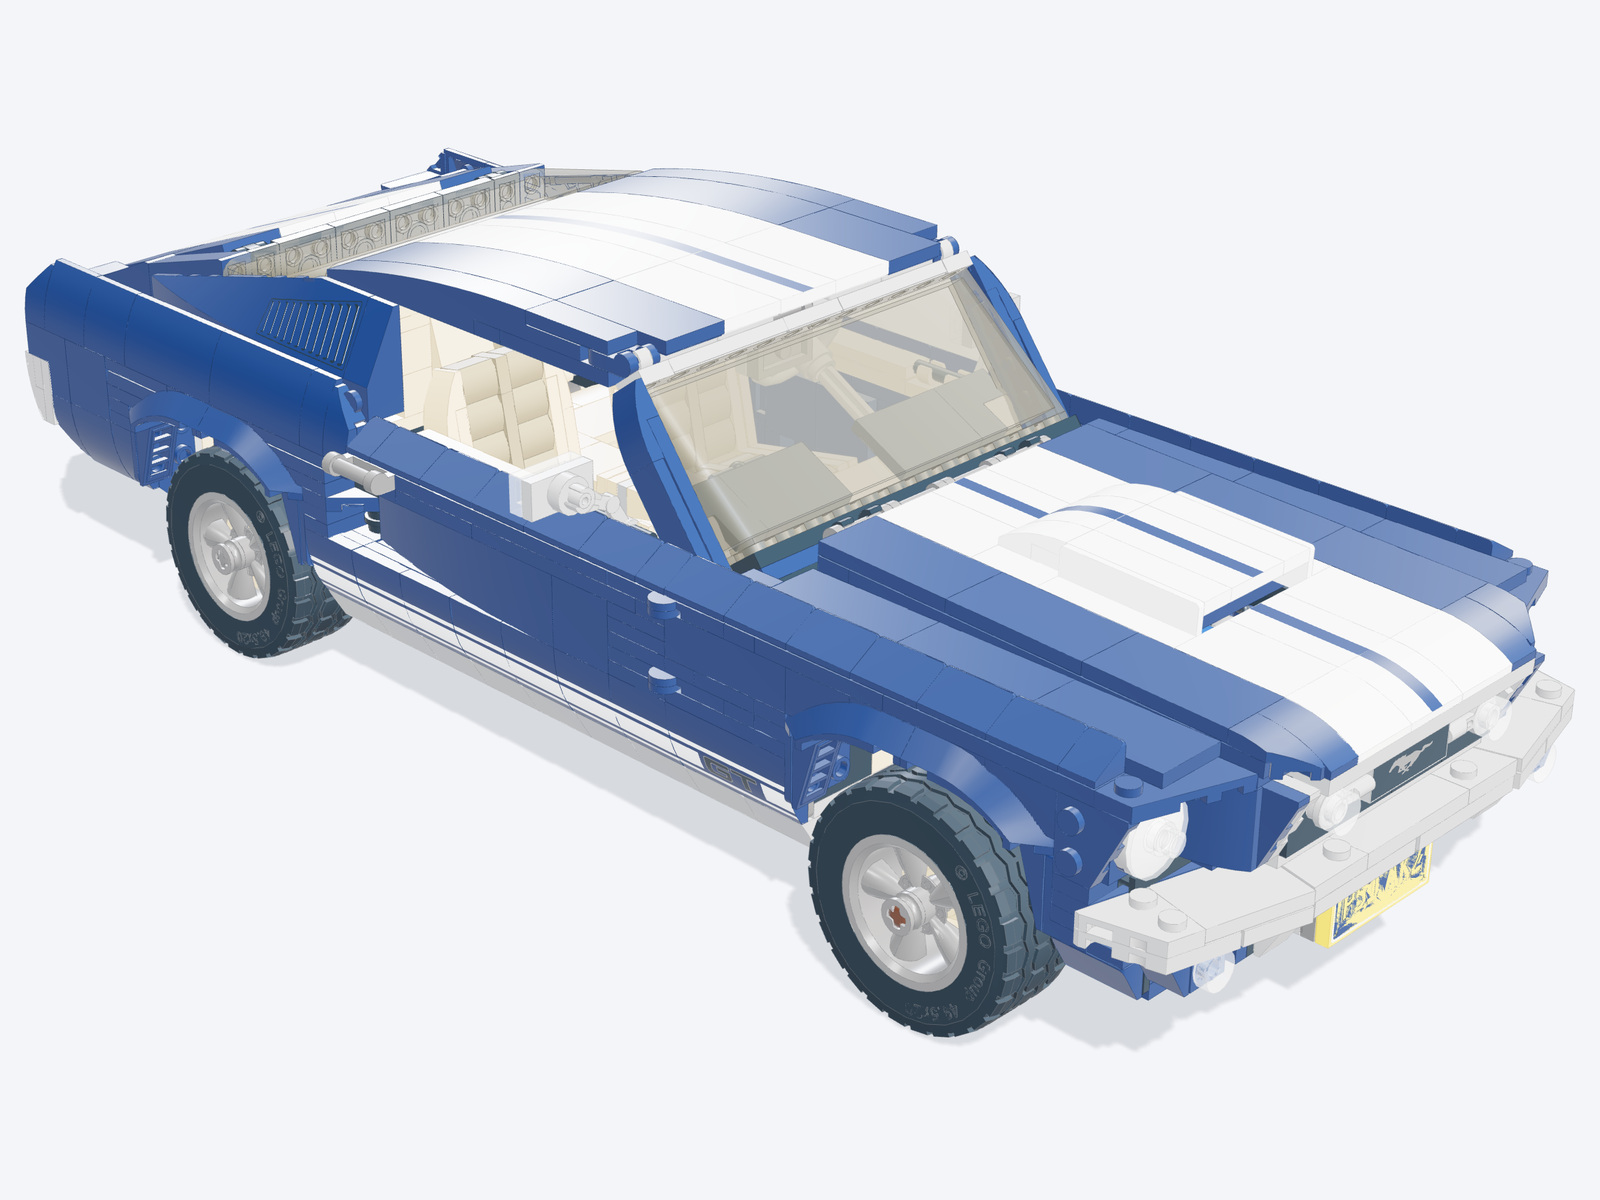
\includegraphics[width=.48\linewidth]{figures/ldraw/print/omr-10265-iso.jpg}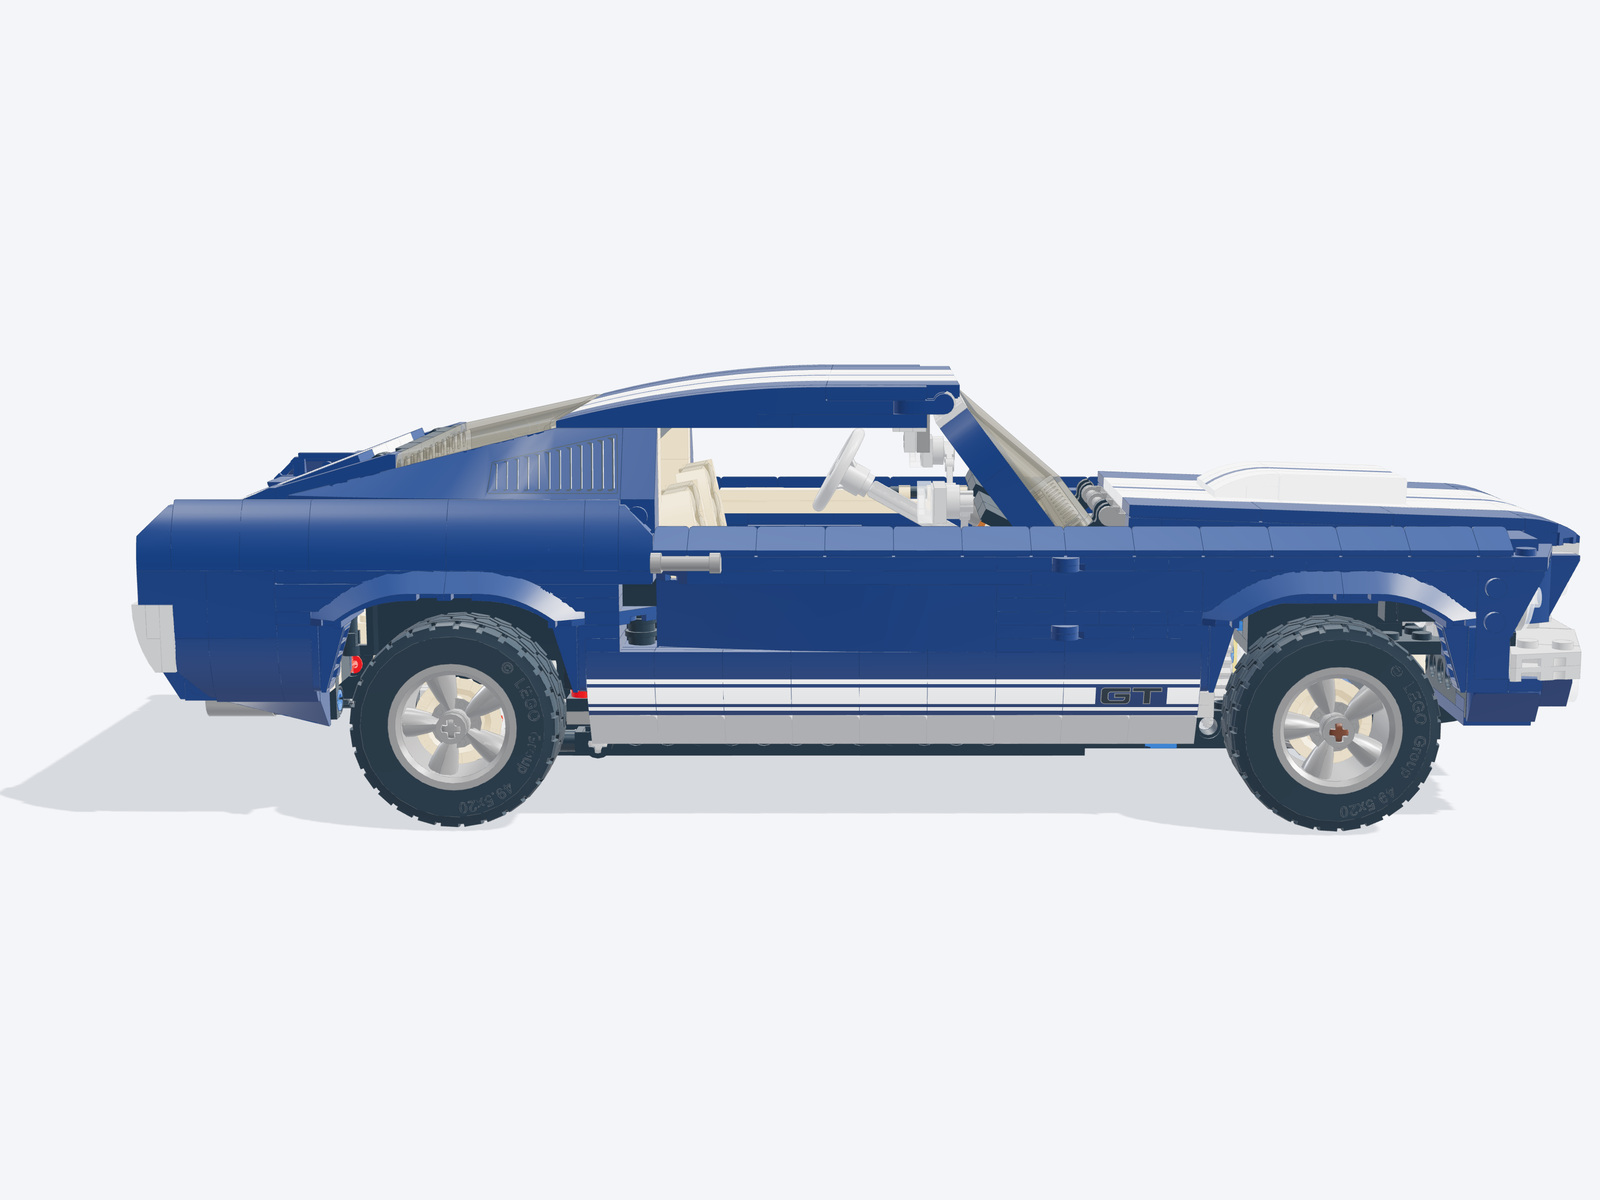
\includegraphics[width=.48\linewidth]{figures/ldraw/print/omr-10265-front.jpg}\\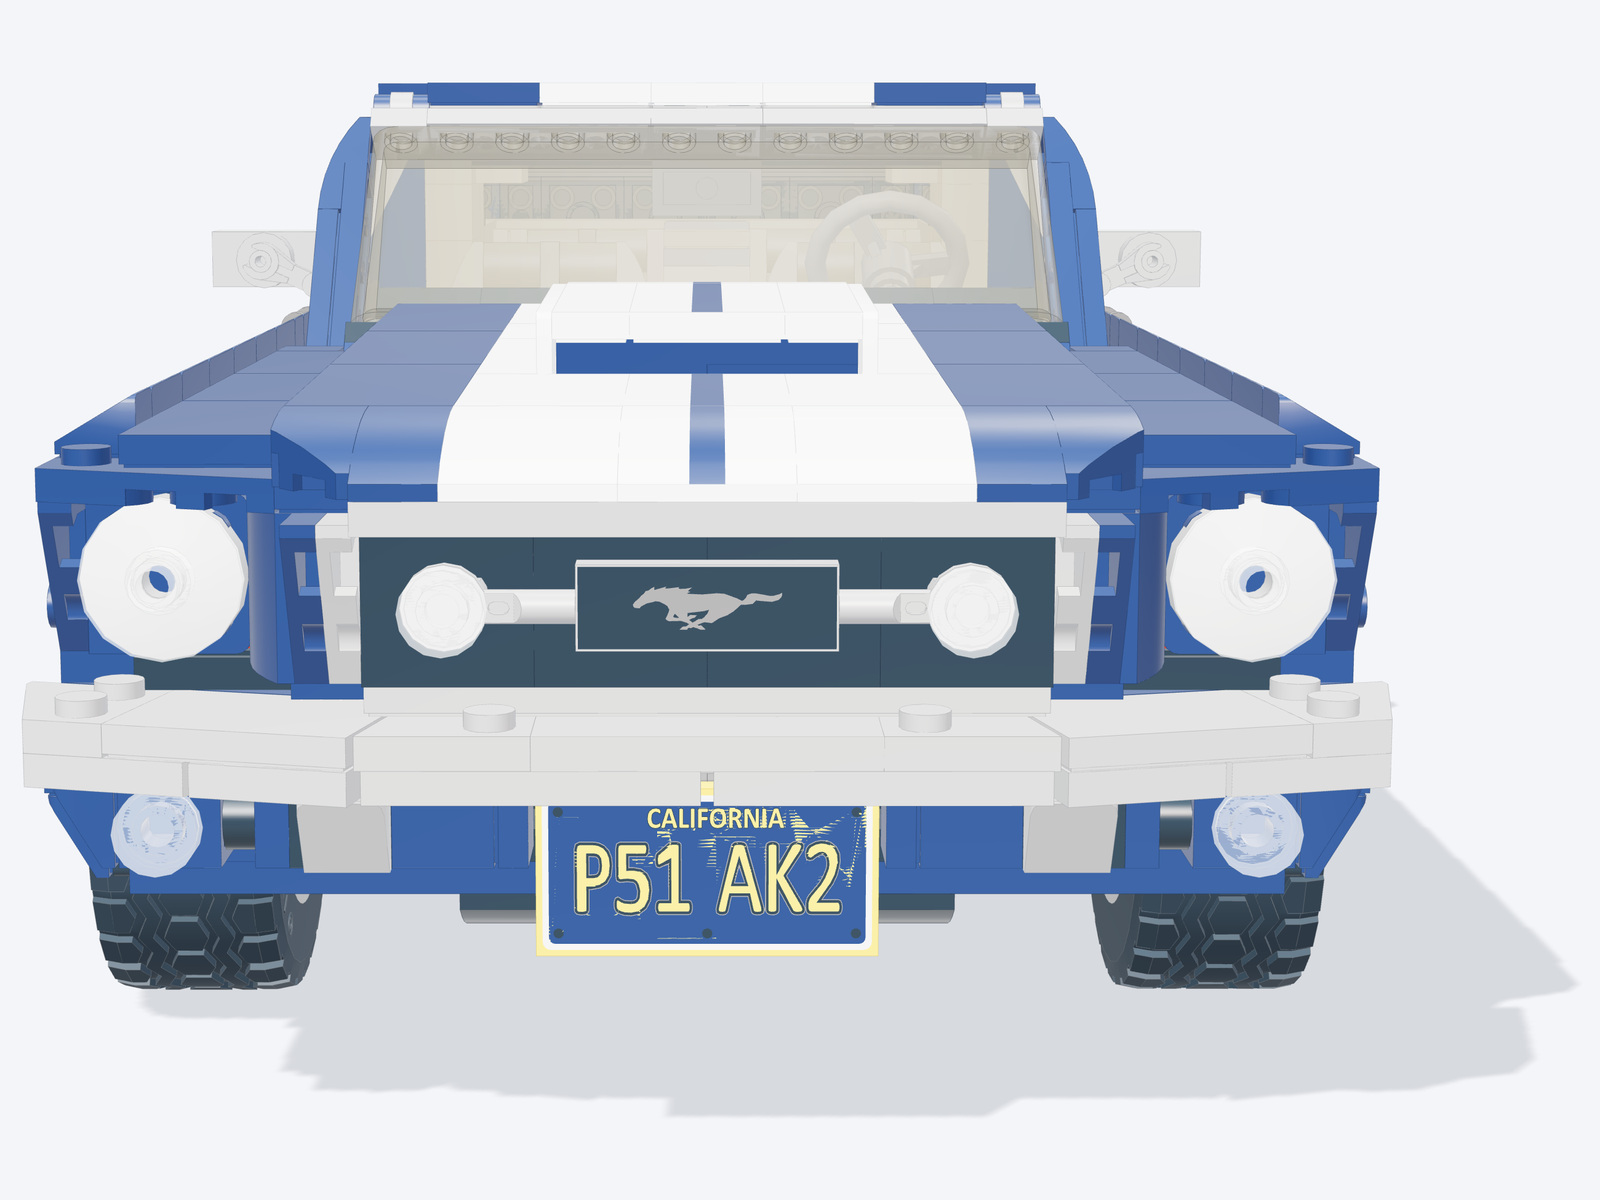
\includegraphics[width=.48\linewidth]{figures/ldraw/print/omr-10265-side.jpg}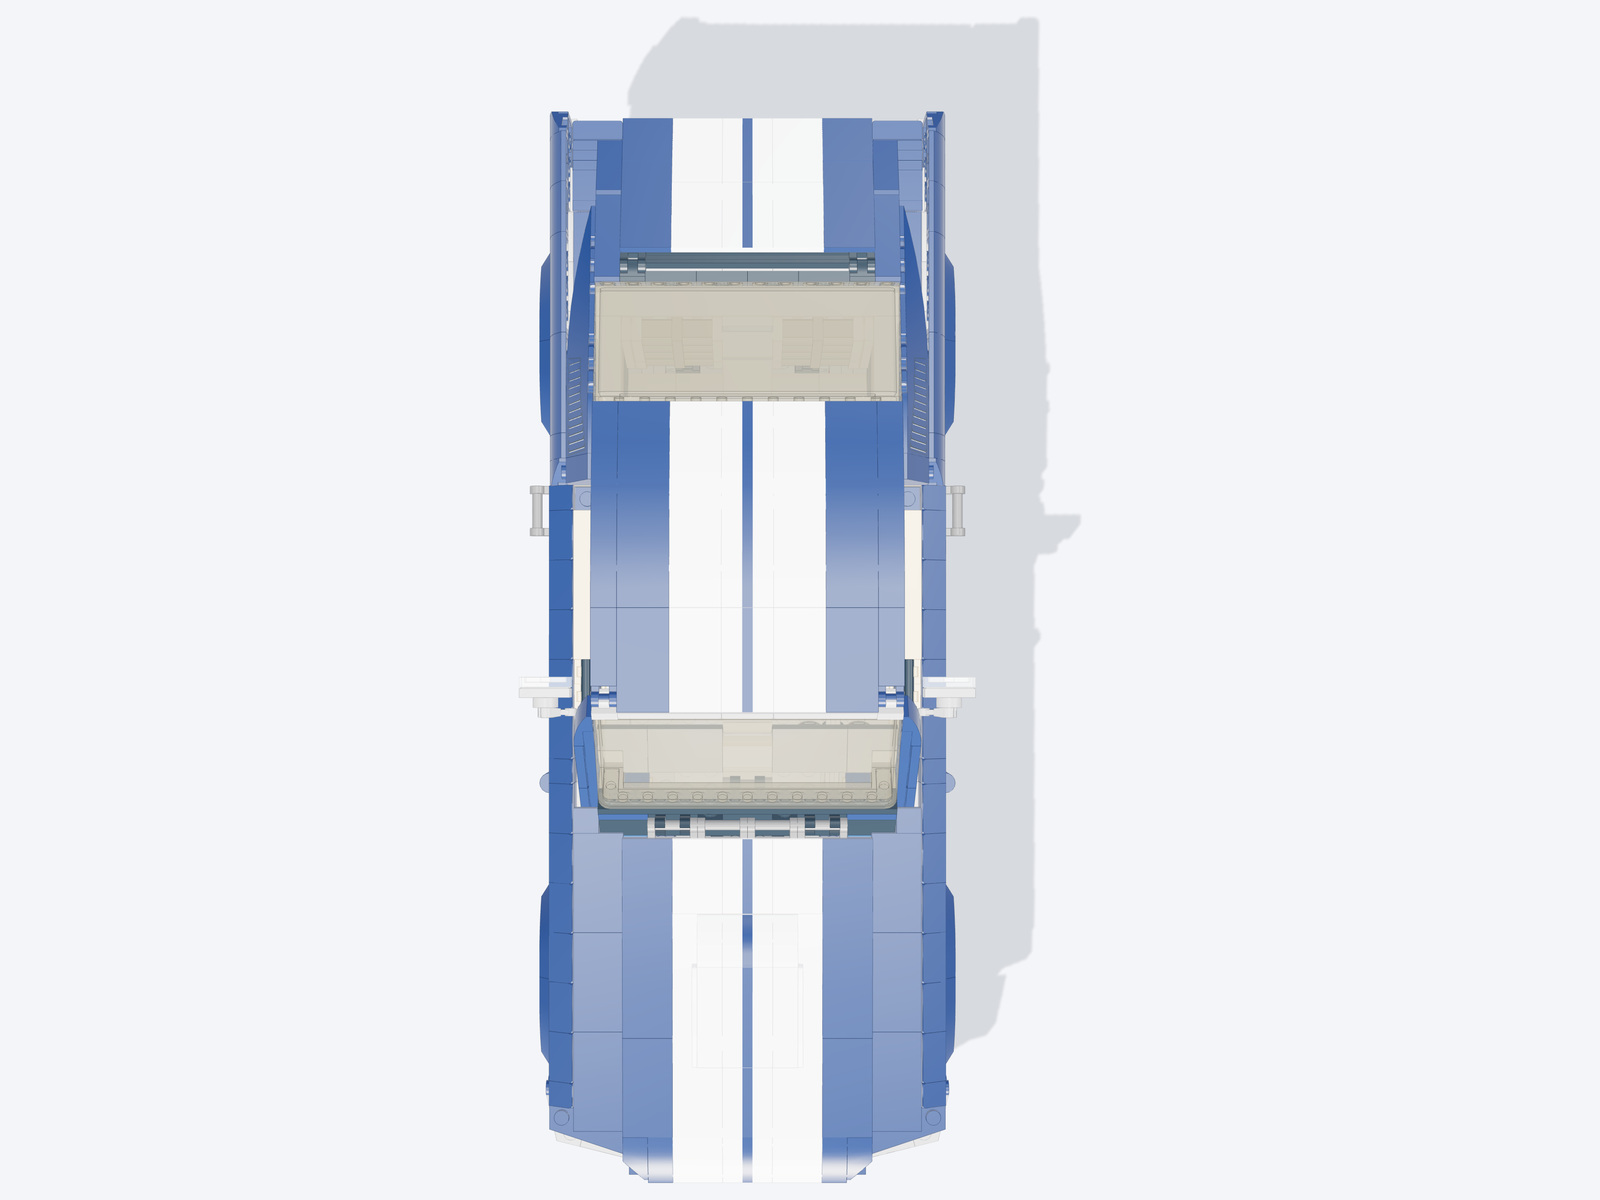
\includegraphics[width=.48\linewidth]{figures/ldraw/print/omr-10265-top.jpg}\end{center}
\paragraph{Attribution.}Ulrich Röder [UR]. CC BY 2.0.\par\noindent\url{https://library.ldraw.org/library/omr/10265-1.mpd}
\paragraph{Source lock.}\small\texttt{e9a2eb1b84d343a6faa9861d186159cf}\\\texttt{5d1fa1e202366eae1e76287df114ea95}\normalsize
\paragraph{Evidence coverage.}Connector definitions cover 99.26\% of instances. The audit reports 27 recognized-graph components and 109 intersection candidates without a recognized mating pair. 10 instances have no connector definition. These counts do not certify physical defects or gravitational stability.
\paragraph{Instructions.}82 expanded author steps.
\clearpage\subsection{Numbered visual input and complete question index}
Only relevant numbers are shown. The website can isolate any instance; public visual tasks provide their own numbered images. The following entries give every English prompt, all choice options, compact public evidence and the reference output. Raw repeated connector records and full action fact sets remain in the versioned JSON.
\begin{center}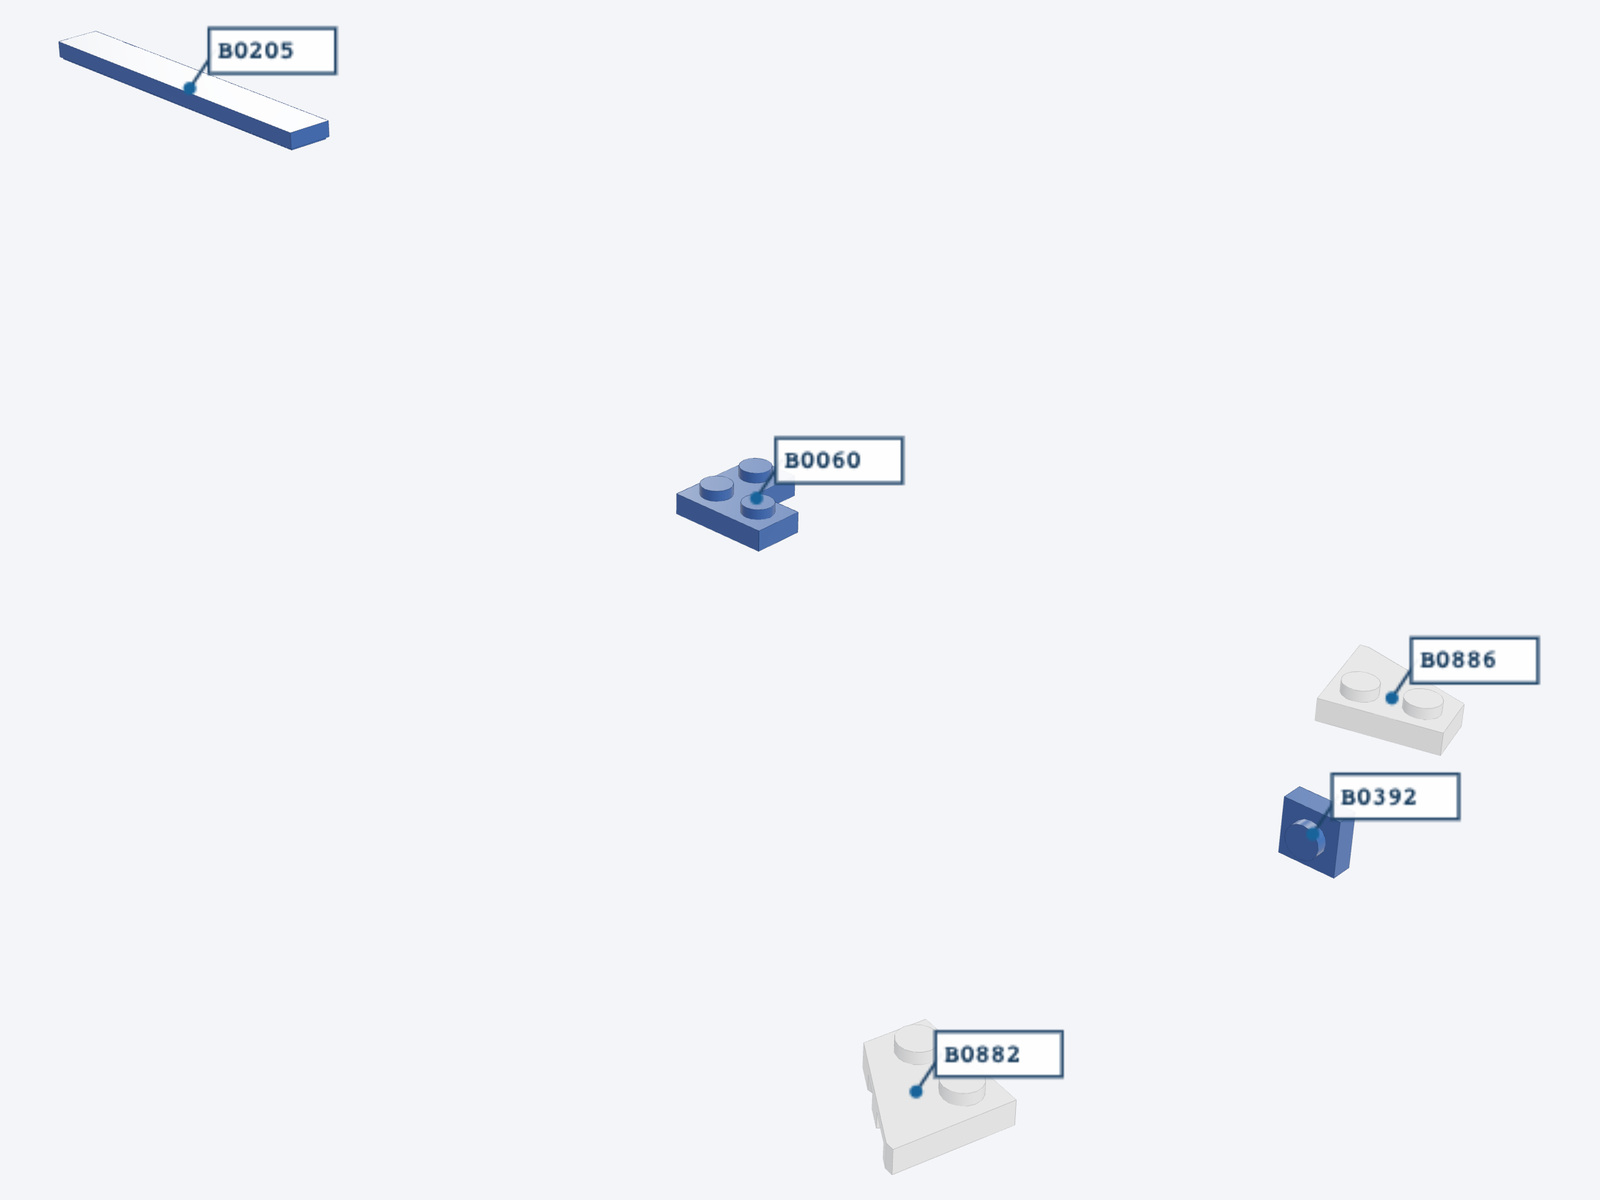
\includegraphics[width=.55\linewidth]{figures/ldraw/print/omr-10265-numbered.jpg}\end{center}
\begin{enumerate}
\item \textbf{color-1}. Identify the original color of B0886; numbered isolation is allowed.\par {\small \textit{Input:} Numbered visual input; source attributes are withheld from the model. \par\textit{Options:} A: Dark Tan; B: Light Bluish Grey; C: Dark Orange; D: Black. \par\textit{Reference output:} B.}
\item \textbf{shape-match-1}. Ignoring color and pose, which numbered instance has the same LDraw part type as B0886?\par {\small \textit{Input:} Numbered visual input; source attributes are withheld from the model. \par\textit{Options:} A: B0205; B: B0060; C: B0392; D: B0882. \par\textit{Reference output:} D.}
\item \textbf{distance-1}. Using the supplied geometry bounding-box centers, which candidate is nearest to B0886?\par {\small \textit{Input:} Centers (mm): B0886 = (59.654664, 31.2, 177.179945); B0275 = (-56, 37.6, 84); B0105 = (56, 50.4, -4); B0599 = (12.1, 21.6, -80). \par\textit{Options:} A: B0275; B: B0599; C: B0105. \par\textit{Reference output:} A.}
\item \textbf{color-2}. Identify the original color of B1090; numbered isolation is allowed.\par {\small \textit{Input:} Numbered visual input; source attributes are withheld from the model. \par\textit{Options:} A: Tan; B: Aqua; C: Trans Red; D: Yellow. \par\textit{Reference output:} A.}
\item \textbf{shape-match-2}. Ignoring color and pose, which numbered instance has the same LDraw part type as B1090?\par {\small \textit{Input:} Numbered visual input; source attributes are withheld from the model. \par\textit{Options:} A: B1209; B: B1089; C: B0527; D: B0425. \par\textit{Reference output:} B.}
\item \textbf{distance-2}. Using the supplied geometry bounding-box centers, which candidate is nearest to B1090?\par {\small \textit{Input:} Centers (mm): B1090 = (48, 56.8, -40); B0398 = (58.32, 21.6, 180); B0057 = (53.6, 24, 24); B1008 = (-27.2, 29.453016, 10.473528). \par\textit{Options:} A: B0057; B: B1008; C: B0398. \par\textit{Reference output:} A.}
\item \textbf{color-3}. Identify the original color of B0079; numbered isolation is allowed.\par {\small \textit{Input:} Numbered visual input; source attributes are withheld from the model. \par\textit{Options:} A: Green; B: Aqua; C: Dark Orange; D: Tan. \par\textit{Reference output:} D.}
\item \textbf{shape-match-3}. Ignoring color and pose, which numbered instance has the same LDraw part type as B0079?\par {\small \textit{Input:} Numbered visual input; source attributes are withheld from the model. \par\textit{Options:} A: B0759; B: B0269; C: B0311; D: B0283. \par\textit{Reference output:} B.}
\item \textbf{distance-3}. Using the supplied geometry bounding-box centers, which candidate is nearest to B0079?\par {\small \textit{Input:} Centers (mm): B0079 = (52, 21.6, 40); B0940 = (20, 32.49576, 70.615832); B1326 = (-48, 34.4, 165.8); B1261 = (-33.524999, 50.4, 116.479116). \par\textit{Options:} A: B0940; B: B1326; C: B1261. \par\textit{Reference output:} A.}
\item \textbf{color-4}. Identify the original color of B0783; numbered isolation is allowed.\par {\small \textit{Input:} Numbered visual input; source attributes are withheld from the model. \par\textit{Options:} A: Blue; B: Light Bluish Grey; C: Brown; D: Yellow. \par\textit{Reference output:} B.}
\item \textbf{shape-match-4}. Ignoring color and pose, which numbered instance has the same LDraw part type as B0783?\par {\small \textit{Input:} Numbered visual input; source attributes are withheld from the model. \par\textit{Options:} A: B0758; B: B0813; C: B0327; D: B1206. \par\textit{Reference output:} A.}
\item \textbf{distance-4}. Using the supplied geometry bounding-box centers, which candidate is nearest to B0783?\par {\small \textit{Input:} Centers (mm): B0783 = (-40, 49.6, 92); B1240 = (40, 52.303984, 68.446956); B0157 = (56, 50.4, 128); B0683 = (-55.92, 12, 40). \par\textit{Options:} A: B0157; B: B1240; C: B0683. \par\textit{Reference output:} C.}
\item \textbf{color-5}. Identify the original color of B1081; numbered isolation is allowed.\par {\small \textit{Input:} Numbered visual input; source attributes are withheld from the model. \par\textit{Options:} A: Dark Bluish Grey; B: Tan; C: Dark Blue; D: Light Grey. \par\textit{Reference output:} A.}
\item \textbf{shape-match-5}. Ignoring color and pose, which numbered instance has the same LDraw part type as B1081?\par {\small \textit{Input:} Numbered visual input; source attributes are withheld from the model. \par\textit{Options:} A: B1265; B: B0546; C: B0528; D: B1065. \par\textit{Reference output:} D.}
\item \textbf{distance-5}. Using the supplied geometry bounding-box centers, which candidate is nearest to B1081?\par {\small \textit{Input:} Centers (mm): B1081 = (-44, 53.6, -80); B0422 = (-24, 85.6, 28); B0379 = (-60.72, 18.4, 168); B0977 = (-24, 54.433218, 54.679544). \par\textit{Options:} A: B0422; B: B0977; C: B0379. \par\textit{Reference output:} A.}
\item \textbf{interface-1}. Classify the supplied connector record for B0013 and B0010. This does not certify load capacity.\par {\small \textit{Input:} Record: family = axle; connector indices = 14, 1. \par\textit{Options:} A: fixed; B: axle; C: ball; D: hinge. \par\textit{Reference output:} B.}
\item \textbf{interface-2}. Classify the supplied connector record for B0548 and B0556. This does not certify load capacity.\par {\small \textit{Input:} Record: family = ball; connector indices = 3, 7. \par\textit{Options:} A: fixed; B: ball; C: axle; D: hinge. \par\textit{Reference output:} B.}
\item \textbf{interface-3}. Classify the supplied connector record for B0064 and B0065. This does not certify load capacity.\par {\small \textit{Input:} Record: family = hinge; connector indices = 1, 2. \par\textit{Options:} A: ball; B: fixed; C: hinge; D: axle. \par\textit{Reference output:} C.}
\item \textbf{interface-4}. Classify the supplied connector record for B0164 and B0165. This does not certify load capacity.\par {\small \textit{Input:} Record: family = stud; connector indices = 12, 7. \par\textit{Options:} A: fixed; B: stud; C: hinge; D: axle; E: ball. \par\textit{Reference output:} B.}
\item \textbf{neighbors-1}. Select every candidate directly adjacent to B0145 in the supplied connector graph.\par {\small \textit{Input:} Unique undirected pairs: B0145 / B0147; B0145 / B0148. \par\textit{Options:} A: B1255; B: B0147; C: B0296; D: B0148. \par\textit{Reference output:} B, D.}
\item \textbf{graph-removal-1}. Delete B0145 and its incident edges from this local graph. How many connected components remain? Do not infer physical extractability.\par {\small \textit{Input:} Nodes: B0145, B0147, B0148, B1255, B0296. Unique undirected pairs: B0145 / B0147; B0145 / B0148. \par\textit{Options:} A: 4; B: 5; C: 6; D: 3. \par\textit{Reference output:} A.}
\item \textbf{neighbors-2}. Select every candidate directly adjacent to B0745 in the supplied connector graph.\par {\small \textit{Input:} Unique undirected pairs: B0740 / B0745; B0745 / B0751. \par\textit{Options:} A: B0740; B: B0367; C: B0751; D: B0772. \par\textit{Reference output:} A, C.}
\item \textbf{graph-removal-2}. Delete B0745 and its incident edges from this local graph. How many connected components remain? Do not infer physical extractability.\par {\small \textit{Input:} Nodes: B0745, B0740, B0751, B0772, B0367. Unique undirected pairs: B0740 / B0745; B0745 / B0751. \par\textit{Options:} A: 5; B: 3; C: 4; D: 6. \par\textit{Reference output:} C.}
\item \textbf{neighbors-3}. Select every candidate directly adjacent to B1252 in the supplied connector graph.\par {\small \textit{Input:} Unique undirected pairs: B1252 / B1257; B1252 / B1258. \par\textit{Options:} A: B1257; B: B1258; C: B0609; D: B0805. \par\textit{Reference output:} A, B.}
\item \textbf{graph-removal-3}. Delete B1252 and its incident edges from this local graph. How many connected components remain? Do not infer physical extractability.\par {\small \textit{Input:} Nodes: B1252, B1257, B1258, B0609, B0805. Unique undirected pairs: B1252 / B1257; B1252 / B1258. \par\textit{Options:} A: 3; B: 5; C: 6; D: 4. \par\textit{Reference output:} D.}
\item \textbf{neighbors-4}. Select every candidate directly adjacent to B1248 in the supplied connector graph.\par {\small \textit{Input:} Unique undirected pairs: B1248 / B1250; B1248 / B1342. \par\textit{Options:} A: B1342; B: B1294; C: B1324; D: B1250. \par\textit{Reference output:} A, D.}
\item \textbf{graph-removal-4}. Delete B1248 and its incident edges from this local graph. How many connected components remain? Do not infer physical extractability.\par {\small \textit{Input:} Nodes: B1248, B1250, B1342, B1324, B1294. Unique undirected pairs: B1248 / B1250; B1248 / B1342. \par\textit{Options:} A: 5; B: 6; C: 4; D: 3. \par\textit{Reference output:} C.}
\item \textbf{neighbors-5}. Select every candidate directly adjacent to B0979 in the supplied connector graph.\par {\small \textit{Input:} Unique undirected pairs: B0964 / B0979; B0979 / B0980. \par\textit{Options:} A: B1133; B: B0964; C: B0980; D: B0719. \par\textit{Reference output:} B, C.}
\item \textbf{graph-removal-5}. Delete B0979 and its incident edges from this local graph. How many connected components remain? Do not infer physical extractability.\par {\small \textit{Input:} Nodes: B0979, B0964, B0980, B0719, B1133. Unique undirected pairs: B0964 / B0979; B0979 / B0980. \par\textit{Options:} A: 4; B: 6; C: 5; D: 3. \par\textit{Reference output:} A.}
\item \textbf{coverage-1}. Which numbered instance lacks a connector definition in the coverage record, so this audit cannot establish that it is floating?\par {\small \textit{Input:} Definition coverage: B0712 = unsupported; B0886 = supported; B1090 = supported; B0079 = supported. \par\textit{Options:} A: B0079; B: B1090; C: B0886; D: B0712. \par\textit{Reference output:} D.}
\item \textbf{evidence-limit-1}. Only source geometry, connector matching and mesh intersection audits are available. Without mass, friction, material or dynamic tests, is gravitational stability established?\par {\small \textit{Input:} Available evidence: Original CAD; Connector inference; Inset-mesh intersection candidates. \par\textit{Options:} A: Established; B: Not established by this evidence. \par\textit{Reference output:} B.}
\item \textbf{source-step-1}. At which expanded author step does B0884 first appear in the supplied source-step table? Source order is not a collision-free assembly proof.\par {\small \textit{Input:} Expanded author records: step 1: B0001; step 54: B0884. \par\textit{Options:} A: 55; B: 53; C: 54; D: 56. \par\textit{Reference output:} C.}
\item \textbf{source-step-2}. At which expanded author step does B0719 first appear in the supplied source-step table? Source order is not a collision-free assembly proof.\par {\small \textit{Input:} Expanded author records: step 1: B0001; step 46: B0719. \par\textit{Options:} A: 45; B: 47; C: 48; D: 46. \par\textit{Reference output:} D.}
\item \textbf{source-step-3}. At which expanded author step does B0531 first appear in the supplied source-step table? Source order is not a collision-free assembly proof.\par {\small \textit{Input:} Expanded author records: step 1: B0001; step 31: B0531. \par\textit{Options:} A: 31; B: 32; C: 30; D: 33. \par\textit{Reference output:} A.}
\item \textbf{source-step-4}. At which expanded author step does B0710 first appear in the supplied source-step table? Source order is not a collision-free assembly proof.\par {\small \textit{Input:} Expanded author records: step 1: B0001; step 45: B0710. \par\textit{Options:} A: 44; B: 45; C: 47; D: 46. \par\textit{Reference output:} B.}
\item \textbf{source-step-5}. At which expanded author step does B0028 first appear in the supplied source-step table? Source order is not a collision-free assembly proof.\par {\small \textit{Input:} Expanded author records: step 1: B0001; step 10: B0028. \par\textit{Options:} A: 11; B: 9; C: 12; D: 10. \par\textit{Reference output:} D.}
\item \textbf{source-sequence-1}. Reveal the supplied source-step window in author order. Actions change visibility only, without simulating insertion trajectories.\par {\small \textit{Input:} Source window: step-1: B0001, B0002, B0003, B0004; step-2: B0005, B0006; step-3: B0007, B0008, B0009, B0010, B0011, B0012; step-4: B0013, B0014; step-5: B0015, B0016, B0017; step-6: B0018. Action budget: 6. \par\textit{Reference output:} step-1, step-2, step-3, step-4, step-5, step-6.}
\item \textbf{restore-instance-1}. The display copy hides B0886. Restore only that numbered instance, preserving all other instances and source poses.\par {\small \textit{Input:} Target: B0886. Action budget: 1. All other instances initially remain visible. \par\textit{Reference output:} restore-B0886.}
\item \textbf{restore-instance-2}. The display copy hides B1090. Restore only that numbered instance, preserving all other instances and source poses.\par {\small \textit{Input:} Target: B1090. Action budget: 1. All other instances initially remain visible. \par\textit{Reference output:} restore-B1090.}
\item \textbf{restore-instance-3}. The display copy hides B0079. Restore only that numbered instance, preserving all other instances and source poses.\par {\small \textit{Input:} Target: B0079. Action budget: 1. All other instances initially remain visible. \par\textit{Reference output:} restore-B0079.}
\end{enumerate}
\clearpage
\section{10220: Volkswagen T1 Camper Van}
1428 source instances; 39 tasks; D4 scale band.

\par\noindent Perspective, front, side and top views follow in reading order. Original source transforms are preserved.
\begin{center}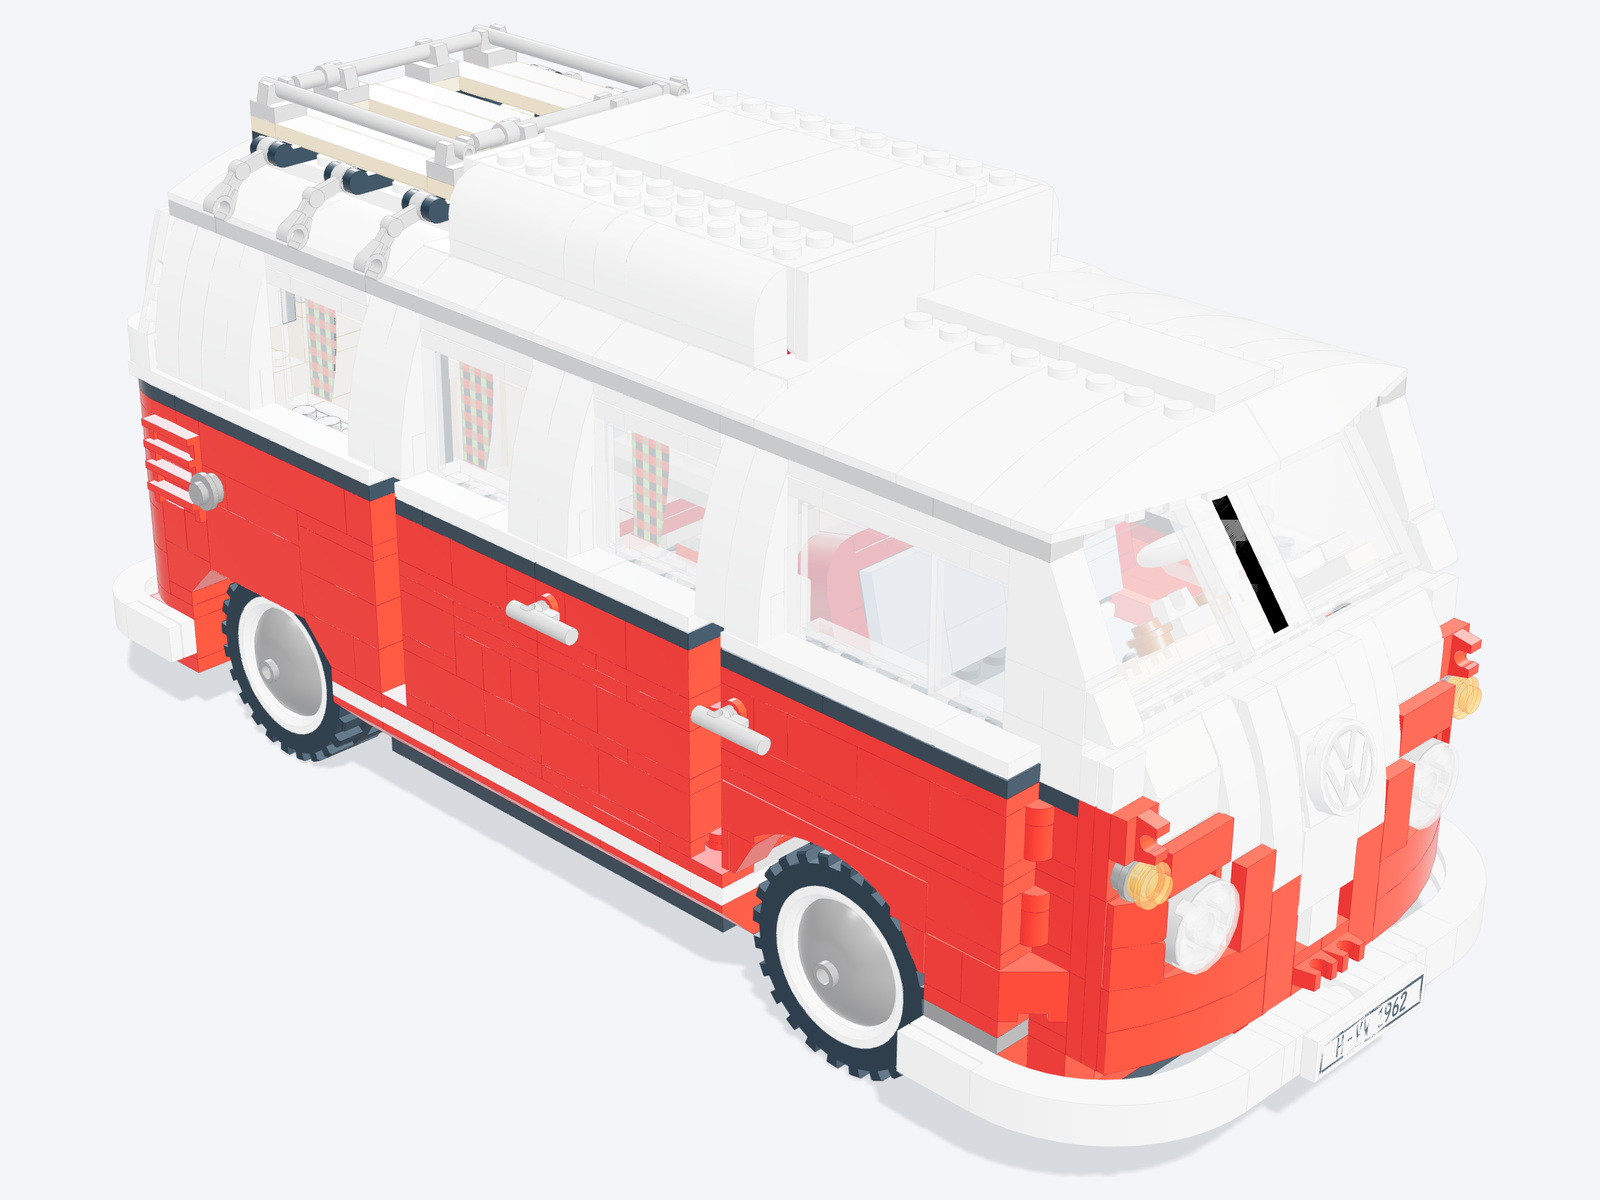
\includegraphics[width=.48\linewidth]{figures/ldraw/print/10220-iso.jpg}
\includegraphics[width=.48\linewidth]{figures/ldraw/print/10220-front.jpg}\\
\includegraphics[width=.48\linewidth]{figures/ldraw/print/10220-side.jpg}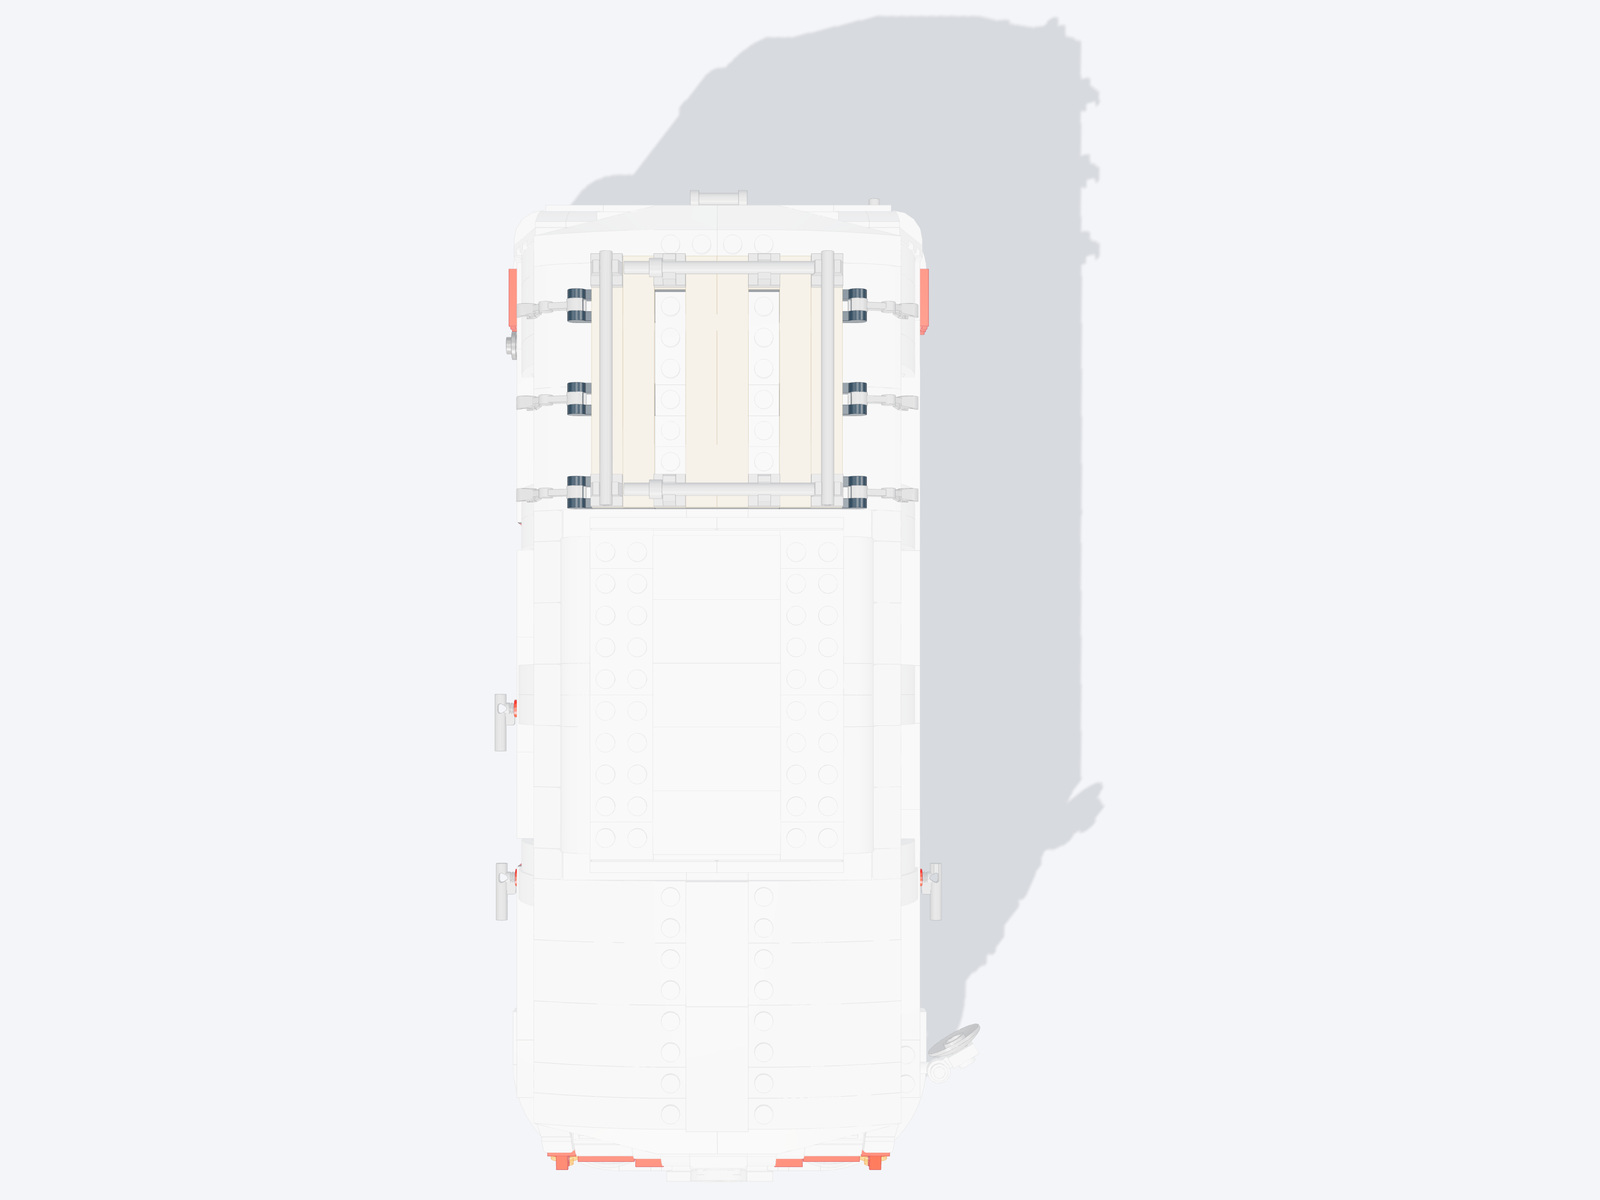
\includegraphics[width=.48\linewidth]{figures/ldraw/print/10220-top.jpg}\end{center}
\paragraph{Attribution.}Stan Isachenko [angmarec]. CC BY 2.0.\par\noindent\url{https://library.ldraw.org/omr/sets/1294}
\paragraph{Source lock.}\small\texttt{ded9a68fc1b569e2965aa67febd225ab}\\\texttt{9d4b496a5d944247488d64c5d1619373}\normalsize
\paragraph{Evidence coverage.}Connector definitions cover 93.00\% of instances. The audit reports 106 recognized-graph components and 7 intersection candidates without a recognized mating pair. 100 instances have no connector definition. These counts do not certify physical defects or gravitational stability.
\paragraph{Instructions.}433 expanded author steps.
\clearpage\subsection{Numbered visual input and complete question index}
Only relevant numbers are shown. The website can isolate any instance; public visual tasks provide their own numbered images. The following entries give every English prompt, all choice options, compact public evidence and the reference output. Raw repeated connector records and full action fact sets remain in the versioned JSON.
\begin{center}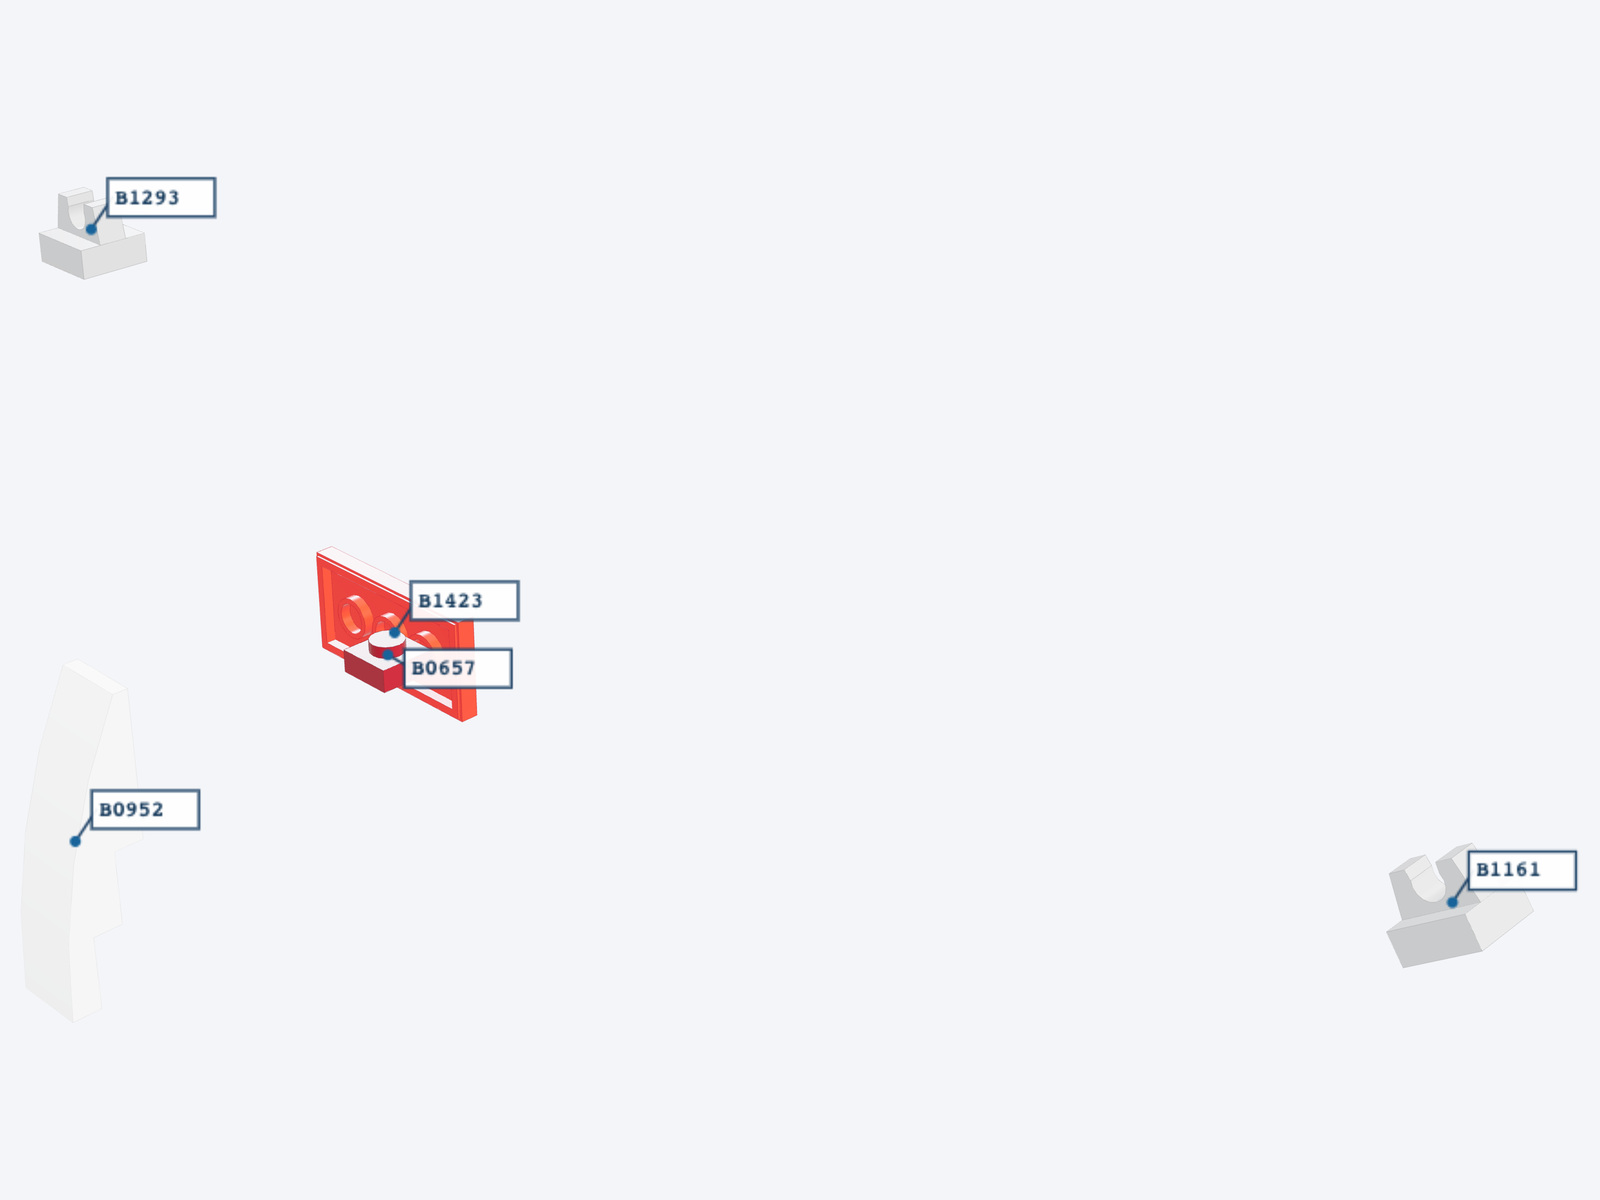
\includegraphics[width=.55\linewidth]{figures/ldraw/print/10220-numbered.jpg}\end{center}
\begin{enumerate}
\item \textbf{color-1}. Identify the original color of B0614; numbered isolation is allowed.\par {\small \textit{Input:} Numbered visual input; source attributes are withheld from the model. \par\textit{Options:} A: Reddish Brown; B: White; C: Dark Red; D: Pearl Gold. \par\textit{Reference output:} A.}
\item \textbf{distance-1}. Using the supplied geometry bounding-box centers, which candidate is nearest to B0614?\par {\small \textit{Input:} Centers (mm): B0614 = (-24, 53.6, 24); B0847 = (48, 63.2, 216); B1232 = (32, 118.4, 152); B0977 = (36, 76, 128). \par\textit{Options:} A: B0847; B: B0977; C: B1232. \par\textit{Reference output:} B.}
\item \textbf{color-2}. Identify the original color of B1293; numbered isolation is allowed.\par {\small \textit{Input:} Numbered visual input; source attributes are withheld from the model. \par\textit{Options:} A: Trans Clear; B: Light Bluish Grey; C: White; D: Bright Light Orange. \par\textit{Reference output:} B.}
\item \textbf{shape-match-1}. Ignoring color and pose, which numbered instance has the same LDraw part type as B1293?\par {\small \textit{Input:} Numbered visual input; source attributes are withheld from the model. \par\textit{Options:} A: B0952; B: B1423; C: B0657; D: B1161. \par\textit{Reference output:} D.}
\item \textbf{distance-2}. Using the supplied geometry bounding-box centers, which candidate is nearest to B1293?\par {\small \textit{Input:} Centers (mm): B1293 = (-12, 122, 76); B1263 = (0, 114.4, 76); B0550 = (-52, 65.6, 156); B0572 = (0, 18.4, 244). \par\textit{Options:} A: B1263; B: B0550; C: B0572. \par\textit{Reference output:} A.}
\item \textbf{color-3}. Identify the original color of B0285; numbered isolation is allowed.\par {\small \textit{Input:} Numbered visual input; source attributes are withheld from the model. \par\textit{Options:} A: Light Bluish Grey; B: Trans Green; C: Red; D: Yellow. \par\textit{Reference output:} C.}
\item \textbf{shape-match-2}. Ignoring color and pose, which numbered instance has the same LDraw part type as B0285?\par {\small \textit{Input:} Numbered visual input; source attributes are withheld from the model. \par\textit{Options:} A: B0780; B: B0479; C: B0415; D: B0874. \par\textit{Reference output:} A.}
\item \textbf{distance-3}. Using the supplied geometry bounding-box centers, which candidate is nearest to B0285?\par {\small \textit{Input:} Centers (mm): B0285 = (-36, 2.4, 244); B0284 = (36, 2.4, 244); B0043 = (25.2, 15.2, 12); B0625 = (8, 45.6, 80.4). \par\textit{Options:} A: B0043; B: B0625; C: B0284. \par\textit{Reference output:} C.}
\item \textbf{color-4}. Identify the original color of B0231; numbered isolation is allowed.\par {\small \textit{Input:} Numbered visual input; source attributes are withheld from the model. \par\textit{Options:} A: Red; B: Bright Light Orange; C: Dark Tan; D: Reddish Brown. \par\textit{Reference output:} A.}
\item \textbf{shape-match-3}. Ignoring color and pose, which numbered instance has the same LDraw part type as B0231?\par {\small \textit{Input:} Numbered visual input; source attributes are withheld from the model. \par\textit{Options:} A: B0485; B: B0743; C: B0747; D: B0255. \par\textit{Reference output:} D.}
\item \textbf{distance-4}. Using the supplied geometry bounding-box centers, which candidate is nearest to B0231?\par {\small \textit{Input:} Centers (mm): B0231 = (-28, 2.4, 120); B0875 = (-32, 72.8, 85.4); B0889 = (-20, 95.2, 68); B1148 = (0, 113.6, 192). \par\textit{Options:} A: B1148; B: B0889; C: B0875. \par\textit{Reference output:} C.}
\item \textbf{color-5}. Identify the original color of B0135; numbered isolation is allowed.\par {\small \textit{Input:} Numbered visual input; source attributes are withheld from the model. \par\textit{Options:} A: Light Bluish Grey; B: Trans Red; C: Tan; D: Yellow. \par\textit{Reference output:} A.}
\item \textbf{shape-match-4}. Ignoring color and pose, which numbered instance has the same LDraw part type as B0135?\par {\small \textit{Input:} Numbered visual input; source attributes are withheld from the model. \par\textit{Options:} A: B0411; B: B0439; C: B0702; D: B0501. \par\textit{Reference output:} D.}
\item \textbf{distance-5}. Using the supplied geometry bounding-box centers, which candidate is nearest to B0135?\par {\small \textit{Input:} Centers (mm): B0135 = (20, 21.6, 44); B0543 = (-58.4, 56.8, 136); B0377 = (-36, 40.8, 4); B0460 = (-36, 31.2, 84). \par\textit{Options:} A: B0543; B: B0377; C: B0460. \par\textit{Reference output:} C.}
\item \textbf{interface-1}. Classify the supplied connector record for B1302 and B1270. This does not certify load capacity.\par {\small \textit{Input:} Record: family = axle; connector indices = 1, 0. \par\textit{Options:} A: ball; B: hinge; C: fixed; D: axle. \par\textit{Reference output:} D.}
\item \textbf{interface-2}. Classify the supplied connector record for B1400 and B1404. This does not certify load capacity.\par {\small \textit{Input:} Record: family = fixed; connector indices = 1, 0. \par\textit{Options:} A: axle; B: hinge; C: fixed; D: ball. \par\textit{Reference output:} C.}
\item \textbf{interface-3}. Classify the supplied connector record for B0492 and B0491. This does not certify load capacity.\par {\small \textit{Input:} Record: family = hinge; connector indices = 1, 2. \par\textit{Options:} A: fixed; B: ball; C: axle; D: hinge. \par\textit{Reference output:} D.}
\item \textbf{interface-4}. Classify the supplied connector record for B0529 and B0542. This does not certify load capacity.\par {\small \textit{Input:} Record: family = stud; connector indices = 4, 0. \par\textit{Options:} A: axle; B: ball; C: fixed; D: stud; E: hinge. \par\textit{Reference output:} D.}
\item \textbf{neighbors-1}. Select every candidate directly adjacent to B1336 in the supplied connector graph.\par {\small \textit{Input:} Unique undirected pairs: B1336 / B1337; B1336 / B1338; B1336 / B1339. \par\textit{Options:} A: B1337; B: B0669; C: B0824; D: B1338; E: B1339. \par\textit{Reference output:} A, D, E.}
\item \textbf{graph-removal-1}. Delete B1336 and its incident edges from this local graph. How many connected components remain? Do not infer physical extractability.\par {\small \textit{Input:} Nodes: B1336, B1337, B1338, B1339, B0824, B0669. Unique undirected pairs: B1336 / B1337; B1336 / B1338; B1336 / B1339. \par\textit{Options:} A: 5; B: 7; C: 6; D: 4. \par\textit{Reference output:} A.}
\item \textbf{neighbors-2}. Select every candidate directly adjacent to B0616 in the supplied connector graph.\par {\small \textit{Input:} Unique undirected pairs: B0601 / B0616; B0616 / B0871. \par\textit{Options:} A: B0601; B: B0871; C: B0501; D: B0120. \par\textit{Reference output:} A, B.}
\item \textbf{graph-removal-2}. Delete B0616 and its incident edges from this local graph. How many connected components remain? Do not infer physical extractability.\par {\small \textit{Input:} Nodes: B0616, B0871, B0601, B0501, B0120. Unique undirected pairs: B0601 / B0616; B0616 / B0871. \par\textit{Options:} A: 6; B: 4; C: 3; D: 5. \par\textit{Reference output:} B.}
\item \textbf{neighbors-3}. Select every candidate directly adjacent to B0563 in the supplied connector graph.\par {\small \textit{Input:} Unique undirected pairs: B0312 / B0563; B0563 / B0566. \par\textit{Options:} A: B0116; B: B0312; C: B0566; D: B0643. \par\textit{Reference output:} B, C.}
\item \textbf{graph-removal-3}. Delete B0563 and its incident edges from this local graph. How many connected components remain? Do not infer physical extractability.\par {\small \textit{Input:} Nodes: B0563, B0566, B0312, B0643, B0116. Unique undirected pairs: B0312 / B0563; B0563 / B0566. \par\textit{Options:} A: 4; B: 6; C: 3; D: 5. \par\textit{Reference output:} A.}
\item \textbf{neighbors-4}. Select every candidate directly adjacent to B0211 in the supplied connector graph.\par {\small \textit{Input:} Unique undirected pairs: B0208 / B0211; B0211 / B0213. \par\textit{Options:} A: B0213; B: B0365; C: B1378; D: B0208. \par\textit{Reference output:} A, D.}
\item \textbf{graph-removal-4}. Delete B0211 and its incident edges from this local graph. How many connected components remain? Do not infer physical extractability.\par {\small \textit{Input:} Nodes: B0211, B0213, B0208, B0365, B1378. Unique undirected pairs: B0208 / B0211; B0211 / B0213. \par\textit{Options:} A: 5; B: 3; C: 4; D: 6. \par\textit{Reference output:} C.}
\item \textbf{neighbors-5}. Select every candidate directly adjacent to B0347 in the supplied connector graph.\par {\small \textit{Input:} Unique undirected pairs: B0338 / B0347; B0347 / B0356; B0347 / B0368. \par\textit{Options:} A: B0368; B: B0344; C: B0357; D: B0356; E: B0338. \par\textit{Reference output:} A, D, E.}
\item \textbf{graph-removal-5}. Delete B0347 and its incident edges from this local graph. How many connected components remain? Do not infer physical extractability.\par {\small \textit{Input:} Nodes: B0347, B0368, B0356, B0338, B0357, B0344. Unique undirected pairs: B0338 / B0347; B0347 / B0356; B0347 / B0368. \par\textit{Options:} A: 5; B: 6; C: 7; D: 4. \par\textit{Reference output:} A.}
\item \textbf{coverage-1}. Which numbered instance lacks a connector definition in the coverage record, so this audit cannot establish that it is floating?\par {\small \textit{Input:} Definition coverage: B0045 = unsupported; B0614 = supported; B1293 = supported; B0285 = supported. \par\textit{Options:} A: B0614; B: B0285; C: B0045; D: B1293. \par\textit{Reference output:} C.}
\item \textbf{evidence-limit-1}. Only source geometry, connector matching and mesh intersection audits are available. Without mass, friction, material or dynamic tests, is gravitational stability established?\par {\small \textit{Input:} Available evidence: Original CAD; Connector inference; Inset-mesh intersection candidates. \par\textit{Options:} A: Not established by this evidence; B: Established. \par\textit{Reference output:} A.}
\item \textbf{source-step-1}. At which expanded author step does B0301 first appear in the supplied source-step table? Source order is not a collision-free assembly proof.\par {\small \textit{Input:} Expanded author records: step 1: B0001; step 71: B0301. \par\textit{Options:} A: 73; B: 70; C: 71; D: 72. \par\textit{Reference output:} C.}
\item \textbf{source-step-2}. At which expanded author step does B1307 first appear in the supplied source-step table? Source order is not a collision-free assembly proof.\par {\small \textit{Input:} Expanded author records: step 1: B0001; step 382: B1307. \par\textit{Options:} A: 384; B: 383; C: 381; D: 382. \par\textit{Reference output:} D.}
\item \textbf{source-step-3}. At which expanded author step does B1400 first appear in the supplied source-step table? Source order is not a collision-free assembly proof.\par {\small \textit{Input:} Expanded author records: step 1: B0001; step 414: B1400. \par\textit{Options:} A: 414; B: 413; C: 416; D: 415. \par\textit{Reference output:} A.}
\item \textbf{source-step-4}. At which expanded author step does B0973 first appear in the supplied source-step table? Source order is not a collision-free assembly proof.\par {\small \textit{Input:} Expanded author records: step 1: B0001; step 266: B0973. \par\textit{Options:} A: 267; B: 265; C: 268; D: 266. \par\textit{Reference output:} D.}
\item \textbf{source-step-5}. At which expanded author step does B1420 first appear in the supplied source-step table? Source order is not a collision-free assembly proof.\par {\small \textit{Input:} Expanded author records: step 1: B0001; step 430: B1420. \par\textit{Options:} A: 429; B: 430; C: 432; D: 431. \par\textit{Reference output:} B.}
\item \textbf{source-sequence-1}. Reveal the supplied source-step window in author order. Actions change visibility only, without simulating insertion trajectories.\par {\small \textit{Input:} Source window: step-1: B0001, B0002; step-2: B0003, B0004, B0005; step-3: B0006, B0007; step-4: B0008, B0009, B0010, B0011, B0012, B0013; step-5: B0014, B0015, B0016, B0017, B0018; step-6: B0019, B0020, B0021, B0022, B0023. Action budget: 6. \par\textit{Reference output:} step-1, step-2, step-3, step-4, step-5, step-6.}
\item \textbf{restore-instance-1}. The display copy hides B0614. Restore only that numbered instance, preserving all other instances and source poses.\par {\small \textit{Input:} Target: B0614. Action budget: 1. All other instances initially remain visible. \par\textit{Reference output:} restore-B0614.}
\item \textbf{restore-instance-2}. The display copy hides B1293. Restore only that numbered instance, preserving all other instances and source poses.\par {\small \textit{Input:} Target: B1293. Action budget: 1. All other instances initially remain visible. \par\textit{Reference output:} restore-B1293.}
\item \textbf{restore-instance-3}. The display copy hides B0285. Restore only that numbered instance, preserving all other instances and source poses.\par {\small \textit{Input:} Target: B0285. Action budget: 1. All other instances initially remain visible. \par\textit{Reference output:} restore-B0285.}
\end{enumerate}
\clearpage
\section{21309: NASA Apollo Saturn V}
1845 source instances; 39 tasks; D4 scale band.

\par\noindent Perspective, front, side and top views follow in reading order. Original source transforms are preserved.
\begin{center}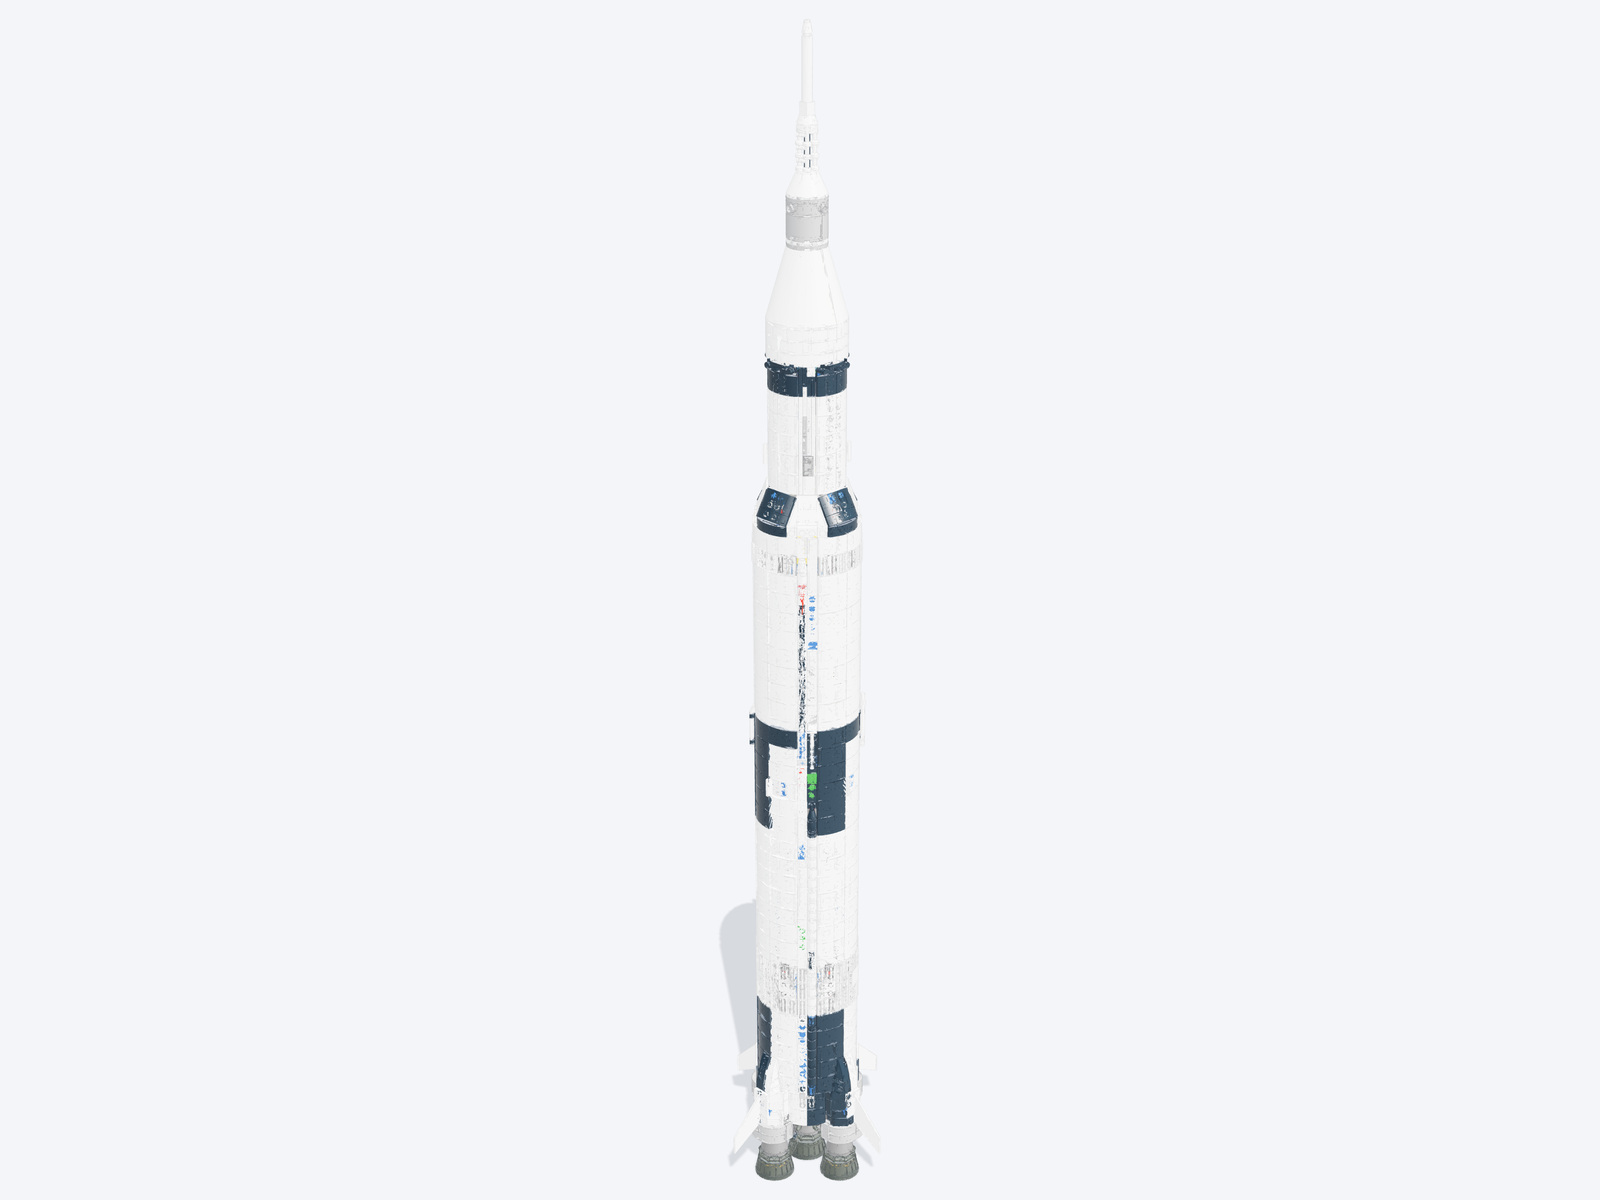
\includegraphics[width=.48\linewidth]{figures/ldraw/print/omr-21309-iso.jpg}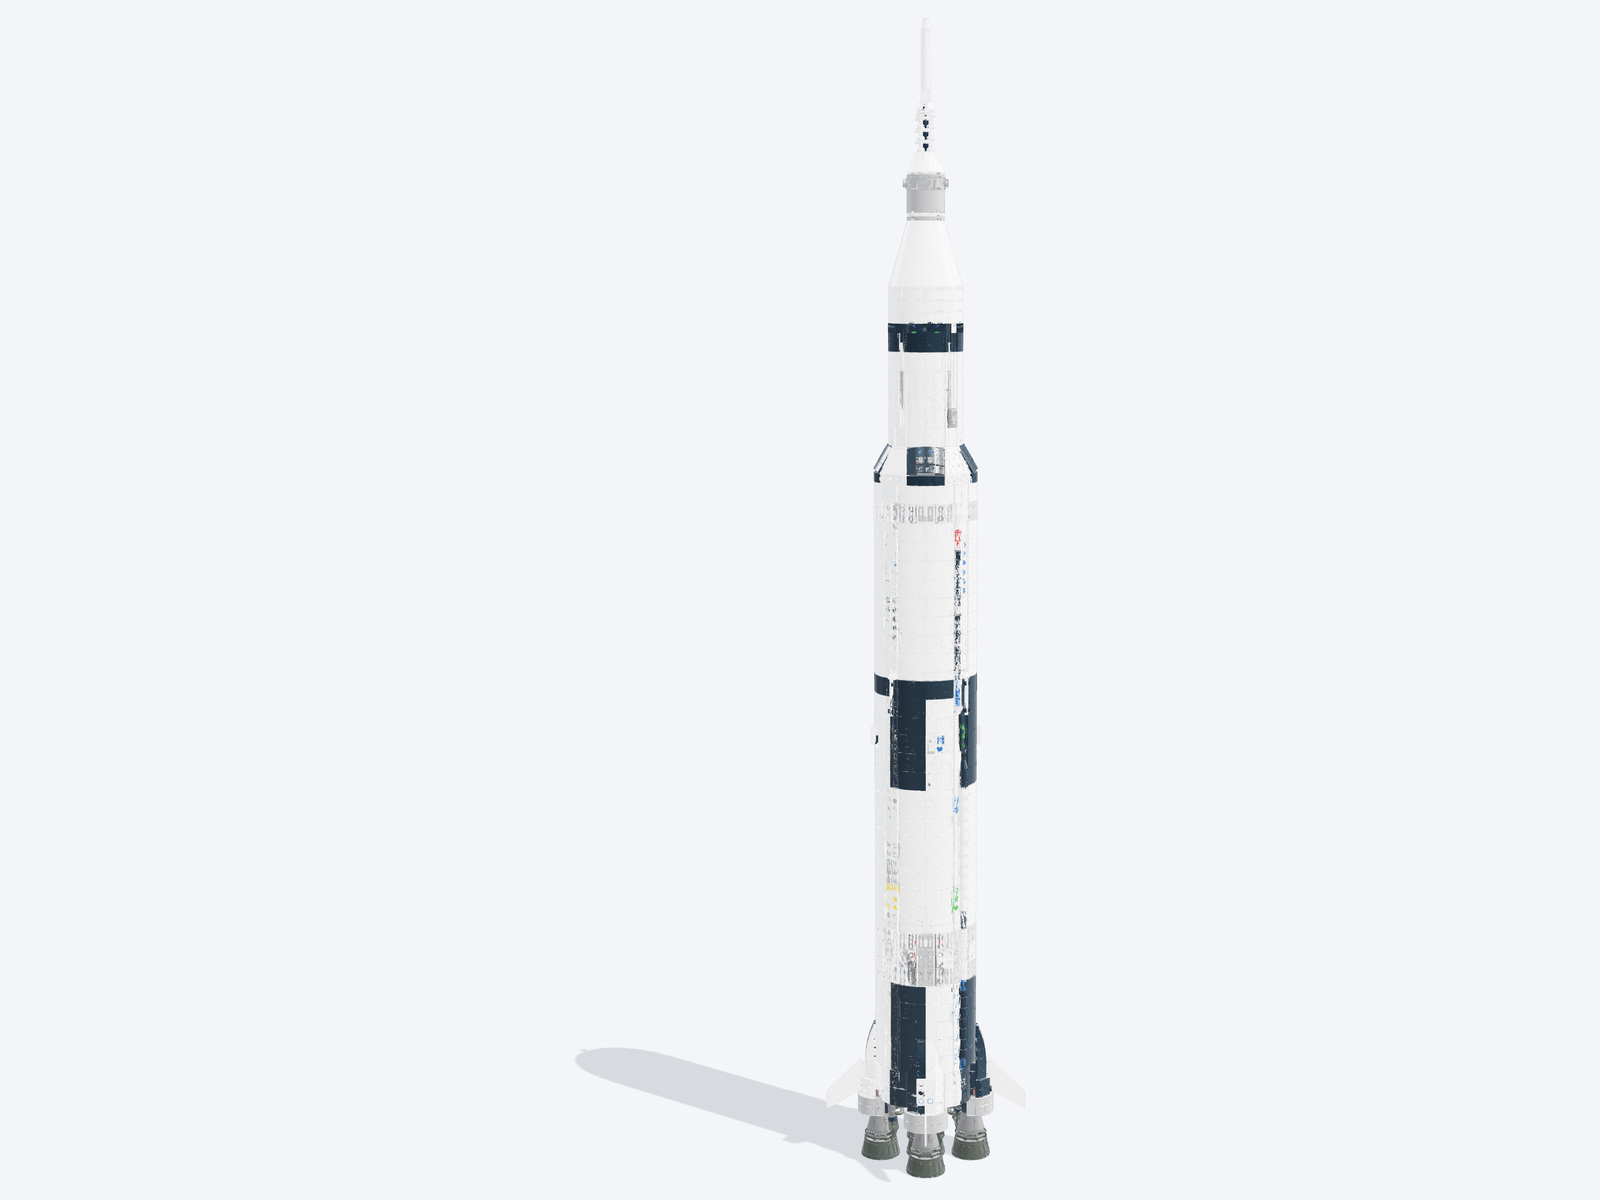
\includegraphics[width=.48\linewidth]{figures/ldraw/print/omr-21309-front.jpg}\\
\includegraphics[width=.48\linewidth]{figures/ldraw/print/omr-21309-side.jpg}
\includegraphics[width=.48\linewidth]{figures/ldraw/print/omr-21309-top.jpg}\end{center}
\paragraph{Attribution.}Jaco van der Molen [Jaco]. CC BY 2.0.\par\noindent\url{https://library.ldraw.org/library/omr/21309-1.mpd}
\paragraph{Source lock.}\small\texttt{eb56995265201179e0ecbad2865fb62f}\\\texttt{ced524c44f3a4179badc964f844e5ba1}\normalsize
\paragraph{Evidence coverage.}Connector definitions cover 100.00\% of instances. The audit reports 9 recognized-graph components and 67 intersection candidates without a recognized mating pair. 0 instances have no connector definition. These counts do not certify physical defects or gravitational stability.
\paragraph{Instructions.}940 expanded author steps.
\clearpage\subsection{Numbered visual input and complete question index}
Only relevant numbers are shown. The website can isolate any instance; public visual tasks provide their own numbered images. The following entries give every English prompt, all choice options, compact public evidence and the reference output. Raw repeated connector records and full action fact sets remain in the versioned JSON.
\begin{center}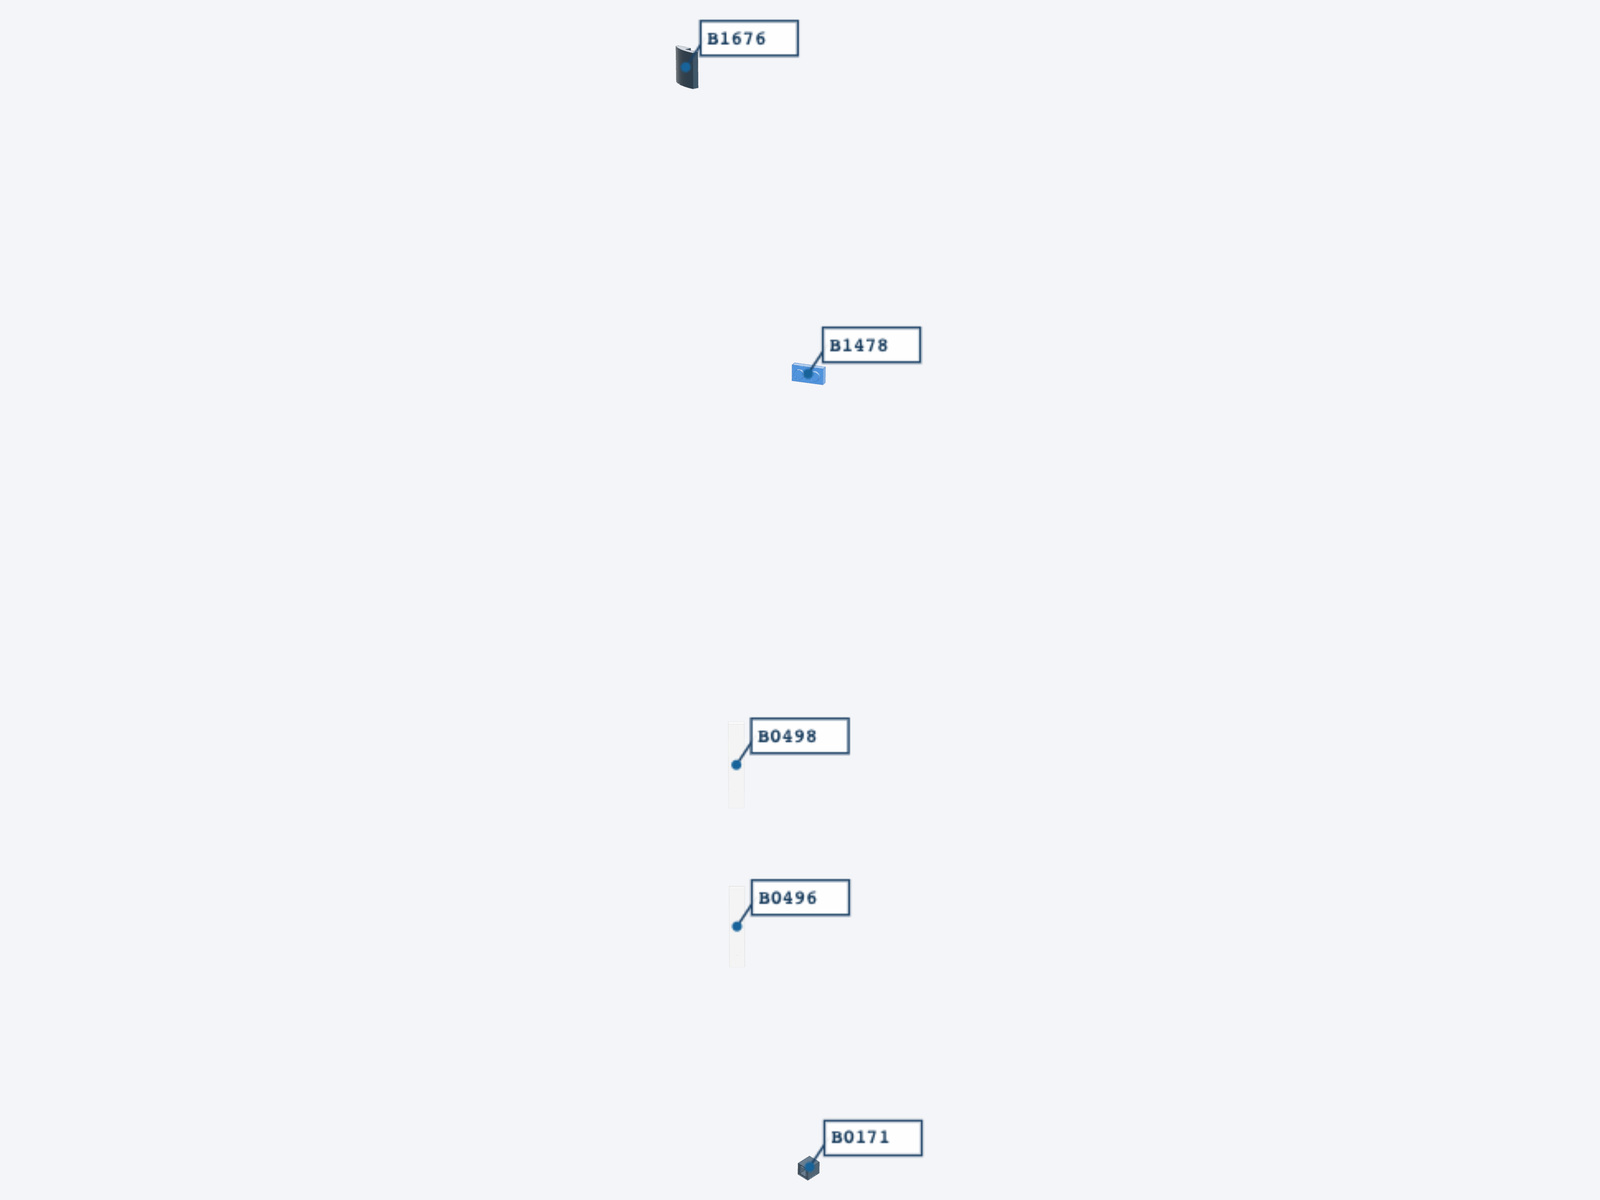
\includegraphics[width=.55\linewidth]{figures/ldraw/print/omr-21309-numbered.jpg}\end{center}
\begin{enumerate}
\item \textbf{color-1}. Identify the original color of B0496; numbered isolation is allowed.\par {\small \textit{Input:} Numbered visual input; source attributes are withheld from the model. \par\textit{Options:} A: Pearl Light Grey; B: Trans Orange; C: White; D: Yellow. \par\textit{Reference output:} C.}
\item \textbf{shape-match-1}. Ignoring color and pose, which numbered instance has the same LDraw part type as B0496?\par {\small \textit{Input:} Numbered visual input; source attributes are withheld from the model. \par\textit{Options:} A: B1478; B: B1676; C: B0498; D: B0171. \par\textit{Reference output:} C.}
\item \textbf{distance-1}. Using the supplied geometry bounding-box centers, which candidate is nearest to B0496?\par {\small \textit{Input:} Centers (mm): B0496 = (-32.5858, 222.4, 26.9286); B1211 = (-33.01, 454.4, 27.354); B1130 = (-20, 532, 0); B0093 = (4, 122.4, -16.4). \par\textit{Options:} A: B1130; B: B1211; C: B0093. \par\textit{Reference output:} C.}
\item \textbf{color-2}. Identify the original color of B0439; numbered isolation is allowed.\par {\small \textit{Input:} Numbered visual input; source attributes are withheld from the model. \par\textit{Options:} A: White; B: Blue; C: Dark Bluish Grey; D: Red. \par\textit{Reference output:} D.}
\item \textbf{shape-match-2}. Ignoring color and pose, which numbered instance has the same LDraw part type as B0439?\par {\small \textit{Input:} Numbered visual input; source attributes are withheld from the model. \par\textit{Options:} A: B0454; B: B1793; C: B0843; D: B0536. \par\textit{Reference output:} A.}
\item \textbf{distance-2}. Using the supplied geometry bounding-box centers, which candidate is nearest to B0439?\par {\small \textit{Input:} Centers (mm): B0439 = (22.2624, 329.20596, 27.9184); B0194 = (40, 154.4, 12); B0642 = (-20.4486, 142.4, -38.3838); B1371 = (-40, 366.4, 12). \par\textit{Options:} A: B0642; B: B1371; C: B0194. \par\textit{Reference output:} B.}
\item \textbf{color-3}. Identify the original color of B1134; numbered isolation is allowed.\par {\small \textit{Input:} Numbered visual input; source attributes are withheld from the model. \par\textit{Options:} A: Yellow; B: Green; C: Black; D: Trans Orange. \par\textit{Reference output:} C.}
\item \textbf{shape-match-3}. Ignoring color and pose, which numbered instance has the same LDraw part type as B1134?\par {\small \textit{Input:} Numbered visual input; source attributes are withheld from the model. \par\textit{Options:} A: B1633; B: B0809; C: B1136; D: B0274. \par\textit{Reference output:} C.}
\item \textbf{distance-3}. Using the supplied geometry bounding-box centers, which candidate is nearest to B1134?\par {\small \textit{Input:} Centers (mm): B1134 = (-20, 538.4, 16.8); B1365 = (-34.4, 534.4, 0); B1800 = (0, 770.39994, 0); B1704 = (0, 570.4, 19.200032). \par\textit{Options:} A: B1704; B: B1365; C: B1800. \par\textit{Reference output:} B.}
\item \textbf{color-4}. Identify the original color of B0754; numbered isolation is allowed.\par {\small \textit{Input:} Numbered visual input; source attributes are withheld from the model. \par\textit{Options:} A: Green; B: Light Bluish Grey; C: Black; D: Pearl Gold. \par\textit{Reference output:} B.}
\item \textbf{shape-match-4}. Ignoring color and pose, which numbered instance has the same LDraw part type as B0754?\par {\small \textit{Input:} Numbered visual input; source attributes are withheld from the model. \par\textit{Options:} A: B0036; B: B0004; C: B0684; D: B0212. \par\textit{Reference output:} C.}
\item \textbf{distance-4}. Using the supplied geometry bounding-box centers, which candidate is nearest to B0754?\par {\small \textit{Input:} Centers (mm): B0754 = (17.3568, 142.4, -33.8352); B1390 = (-40, 486.4, -12); B0068 = (27.3536, 54.4, 27.3536); B1554 = (8, 566.264406, -34.264011). \par\textit{Options:} A: B0068; B: B1554; C: B1390. \par\textit{Reference output:} A.}
\item \textbf{color-5}. Identify the original color of B1147; numbered isolation is allowed.\par {\small \textit{Input:} Numbered visual input; source attributes are withheld from the model. \par\textit{Options:} A: Trans Orange; B: Red; C: Black; D: Blue. \par\textit{Reference output:} D.}
\item \textbf{shape-match-5}. Ignoring color and pose, which numbered instance has the same LDraw part type as B1147?\par {\small \textit{Input:} Numbered visual input; source attributes are withheld from the model. \par\textit{Options:} A: B1154; B: B1175; C: B1410; D: B1740. \par\textit{Reference output:} D.}
\item \textbf{distance-5}. Using the supplied geometry bounding-box centers, which candidate is nearest to B1147?\par {\small \textit{Input:} Centers (mm): B1147 = (0, 340, 12); B1750 = (17.7936, 602.4, -18.7872); B0920 = (-26.2216, 6.4, 26.2216); B1765 = (8, 646.4, 28.800012). \par\textit{Options:} A: B1750; B: B0920; C: B1765. \par\textit{Reference output:} A.}
\item \textbf{interface-1}. Classify the supplied connector record for B0478 and B0477. This does not certify load capacity.\par {\small \textit{Input:} Record: family = axle; connector indices = 1, 0. \par\textit{Options:} A: hinge; B: fixed; C: axle; D: ball. \par\textit{Reference output:} C.}
\item \textbf{interface-2}. Classify the supplied connector record for B1615 and B1737. This does not certify load capacity.\par {\small \textit{Input:} Record: family = ball; connector indices = 3, 3. \par\textit{Options:} A: ball; B: fixed; C: hinge; D: axle. \par\textit{Reference output:} A.}
\item \textbf{interface-3}. Classify the supplied connector record for B0204 and B0868. This does not certify load capacity.\par {\small \textit{Input:} Record: family = hinge; connector indices = 1, 1. \par\textit{Options:} A: axle; B: hinge; C: fixed; D: ball. \par\textit{Reference output:} B.}
\item \textbf{interface-4}. Classify the supplied connector record for B0965 and B0967. This does not certify load capacity.\par {\small \textit{Input:} Record: family = stud; connector indices = 13, 3. \par\textit{Options:} A: axle; B: ball; C: hinge; D: fixed; E: stud. \par\textit{Reference output:} E.}
\item \textbf{neighbors-1}. Select every candidate directly adjacent to B1441 in the supplied connector graph.\par {\small \textit{Input:} Unique undirected pairs: B1435 / B1437; B1435 / B1441; B1437 / B1441. \par\textit{Options:} A: B1549; B: B1437; C: B0432; D: B1435. \par\textit{Reference output:} B, D.}
\item \textbf{graph-removal-1}. Delete B1441 and its incident edges from this local graph. How many connected components remain? Do not infer physical extractability.\par {\small \textit{Input:} Nodes: B1441, B1435, B1437, B1549, B0432. Unique undirected pairs: B1435 / B1437; B1435 / B1441; B1437 / B1441. \par\textit{Options:} A: 3; B: 4; C: 2; D: 5. \par\textit{Reference output:} A.}
\item \textbf{neighbors-2}. Select every candidate directly adjacent to B1250 in the supplied connector graph.\par {\small \textit{Input:} Unique undirected pairs: B0989 / B1250; B1019 / B1250; B1250 / B1251; B1250 / B1252; B1250 / B1253. \par\textit{Options:} A: B1252; B: B1231; C: B1253; D: B0989; E: B1831; F: B1019; G: B1251. \par\textit{Reference output:} A, C, D, F, G.}
\item \textbf{graph-removal-2}. Delete B1250 and its incident edges from this local graph. How many connected components remain? Do not infer physical extractability.\par {\small \textit{Input:} Nodes: B1250, B1019, B1251, B1252, B1253, B0989, B1831, B1231. Unique undirected pairs: B0989 / B1250; B1019 / B1250; B1250 / B1251; B1250 / B1252; B1250 / B1253. \par\textit{Options:} A: 8; B: 7; C: 6; D: 9. \par\textit{Reference output:} B.}
\item \textbf{neighbors-3}. Select every candidate directly adjacent to B1039 in the supplied connector graph.\par {\small \textit{Input:} Unique undirected pairs: B1038 / B1039; B1039 / B1040. \par\textit{Options:} A: B1040; B: B1038; C: B1422; D: B0670. \par\textit{Reference output:} A, B.}
\item \textbf{graph-removal-3}. Delete B1039 and its incident edges from this local graph. How many connected components remain? Do not infer physical extractability.\par {\small \textit{Input:} Nodes: B1039, B1038, B1040, B0670, B1422. Unique undirected pairs: B1038 / B1039; B1039 / B1040. \par\textit{Options:} A: 6; B: 4; C: 5; D: 3. \par\textit{Reference output:} B.}
\item \textbf{neighbors-4}. Select every candidate directly adjacent to B0435 in the supplied connector graph.\par {\small \textit{Input:} Unique undirected pairs: B0424 / B0435; B0435 / B0484; B0435 / B0485; B0435 / B0499. \par\textit{Options:} A: B0485; B: B0424; C: B0657; D: B0499; E: B0193; F: B0484. \par\textit{Reference output:} A, B, D, F.}
\item \textbf{graph-removal-4}. Delete B0435 and its incident edges from this local graph. How many connected components remain? Do not infer physical extractability.\par {\small \textit{Input:} Nodes: B0435, B0484, B0499, B0485, B0424, B0657, B0193. Unique undirected pairs: B0424 / B0435; B0435 / B0484; B0435 / B0485; B0435 / B0499. \par\textit{Options:} A: 6; B: 5; C: 7; D: 8. \par\textit{Reference output:} A.}
\item \textbf{neighbors-5}. Select every candidate directly adjacent to B1053 in the supplied connector graph.\par {\small \textit{Input:} Unique undirected pairs: B1053 / B1054; B1053 / B1055. \par\textit{Options:} A: B1054; B: B0416; C: B1055; D: B0538. \par\textit{Reference output:} A, C.}
\item \textbf{graph-removal-5}. Delete B1053 and its incident edges from this local graph. How many connected components remain? Do not infer physical extractability.\par {\small \textit{Input:} Nodes: B1053, B1054, B1055, B0538, B0416. Unique undirected pairs: B1053 / B1054; B1053 / B1055. \par\textit{Options:} A: 6; B: 4; C: 5; D: 3. \par\textit{Reference output:} B.}
\item \textbf{evidence-limit-1}. Only source geometry, connector matching and mesh intersection audits are available. Without mass, friction, material or dynamic tests, is gravitational stability established?\par {\small \textit{Input:} Available evidence: Original CAD; Connector inference; Inset-mesh intersection candidates. \par\textit{Options:} A: Established; B: Not established by this evidence. \par\textit{Reference output:} B.}
\item \textbf{source-step-1}. At which expanded author step does B1797 first appear in the supplied source-step table? Source order is not a collision-free assembly proof.\par {\small \textit{Input:} Expanded author records: step 1: B0001; step 915: B1797. \par\textit{Options:} A: 914; B: 915; C: 917; D: 916. \par\textit{Reference output:} B.}
\item \textbf{source-step-2}. At which expanded author step does B1075 first appear in the supplied source-step table? Source order is not a collision-free assembly proof.\par {\small \textit{Input:} Expanded author records: step 1: B0001; step 526: B1075. \par\textit{Options:} A: 525; B: 528; C: 527; D: 526. \par\textit{Reference output:} D.}
\item \textbf{source-step-3}. At which expanded author step does B0649 first appear in the supplied source-step table? Source order is not a collision-free assembly proof.\par {\small \textit{Input:} Expanded author records: step 1: B0001; step 285: B0649. \par\textit{Options:} A: 284; B: 287; C: 285; D: 286. \par\textit{Reference output:} C.}
\item \textbf{source-step-4}. At which expanded author step does B1156 first appear in the supplied source-step table? Source order is not a collision-free assembly proof.\par {\small \textit{Input:} Expanded author records: step 1: B0001; step 576: B1156. \par\textit{Options:} A: 575; B: 577; C: 578; D: 576. \par\textit{Reference output:} D.}
\item \textbf{source-step-5}. At which expanded author step does B0131 first appear in the supplied source-step table? Source order is not a collision-free assembly proof.\par {\small \textit{Input:} Expanded author records: step 1: B0001; step 74: B0131. \par\textit{Options:} A: 76; B: 75; C: 74; D: 73. \par\textit{Reference output:} C.}
\item \textbf{source-sequence-1}. Reveal the supplied source-step window in author order. Actions change visibility only, without simulating insertion trajectories.\par {\small \textit{Input:} Source window: step-1: B0001, B0002; step-2: B0003; step-3: B0004; step-4: B0005; step-5: B0006; step-6: B0007. Action budget: 6. \par\textit{Reference output:} step-1, step-2, step-3, step-4, step-5, step-6.}
\item \textbf{restore-instance-1}. The display copy hides B0496. Restore only that numbered instance, preserving all other instances and source poses.\par {\small \textit{Input:} Target: B0496. Action budget: 1. All other instances initially remain visible. \par\textit{Reference output:} restore-B0496.}
\item \textbf{restore-instance-2}. The display copy hides B0439. Restore only that numbered instance, preserving all other instances and source poses.\par {\small \textit{Input:} Target: B0439. Action budget: 1. All other instances initially remain visible. \par\textit{Reference output:} restore-B0439.}
\item \textbf{restore-instance-3}. The display copy hides B1134. Restore only that numbered instance, preserving all other instances and source poses.\par {\small \textit{Input:} Target: B1134. Action budget: 1. All other instances initially remain visible. \par\textit{Reference output:} restore-B1134.}
\end{enumerate}
\clearpage
\section{42054: CLAAS XERION 5000 TRAC VC}
1978 source instances; 39 tasks; D4 scale band.

\par\noindent Perspective, front, side and top views follow in reading order. Original source transforms are preserved.
\begin{center}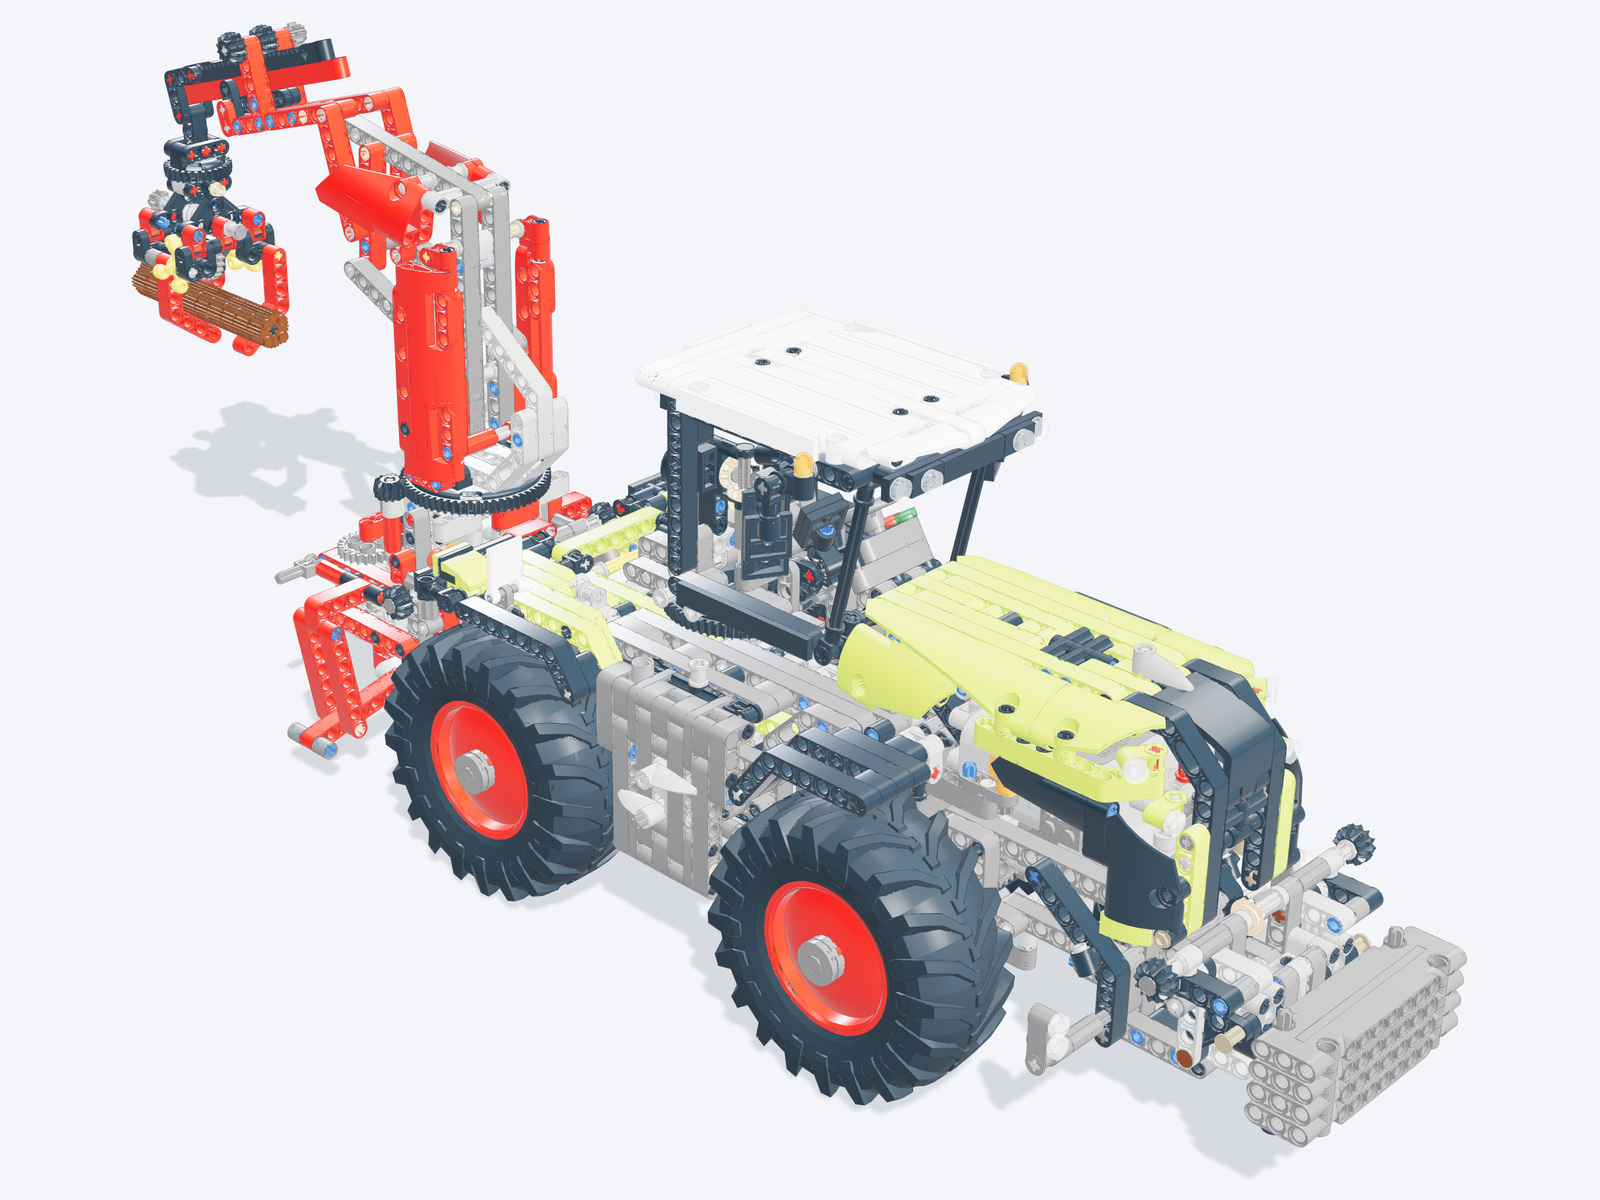
\includegraphics[width=.48\linewidth]{figures/ldraw/print/omr-42054-iso.jpg}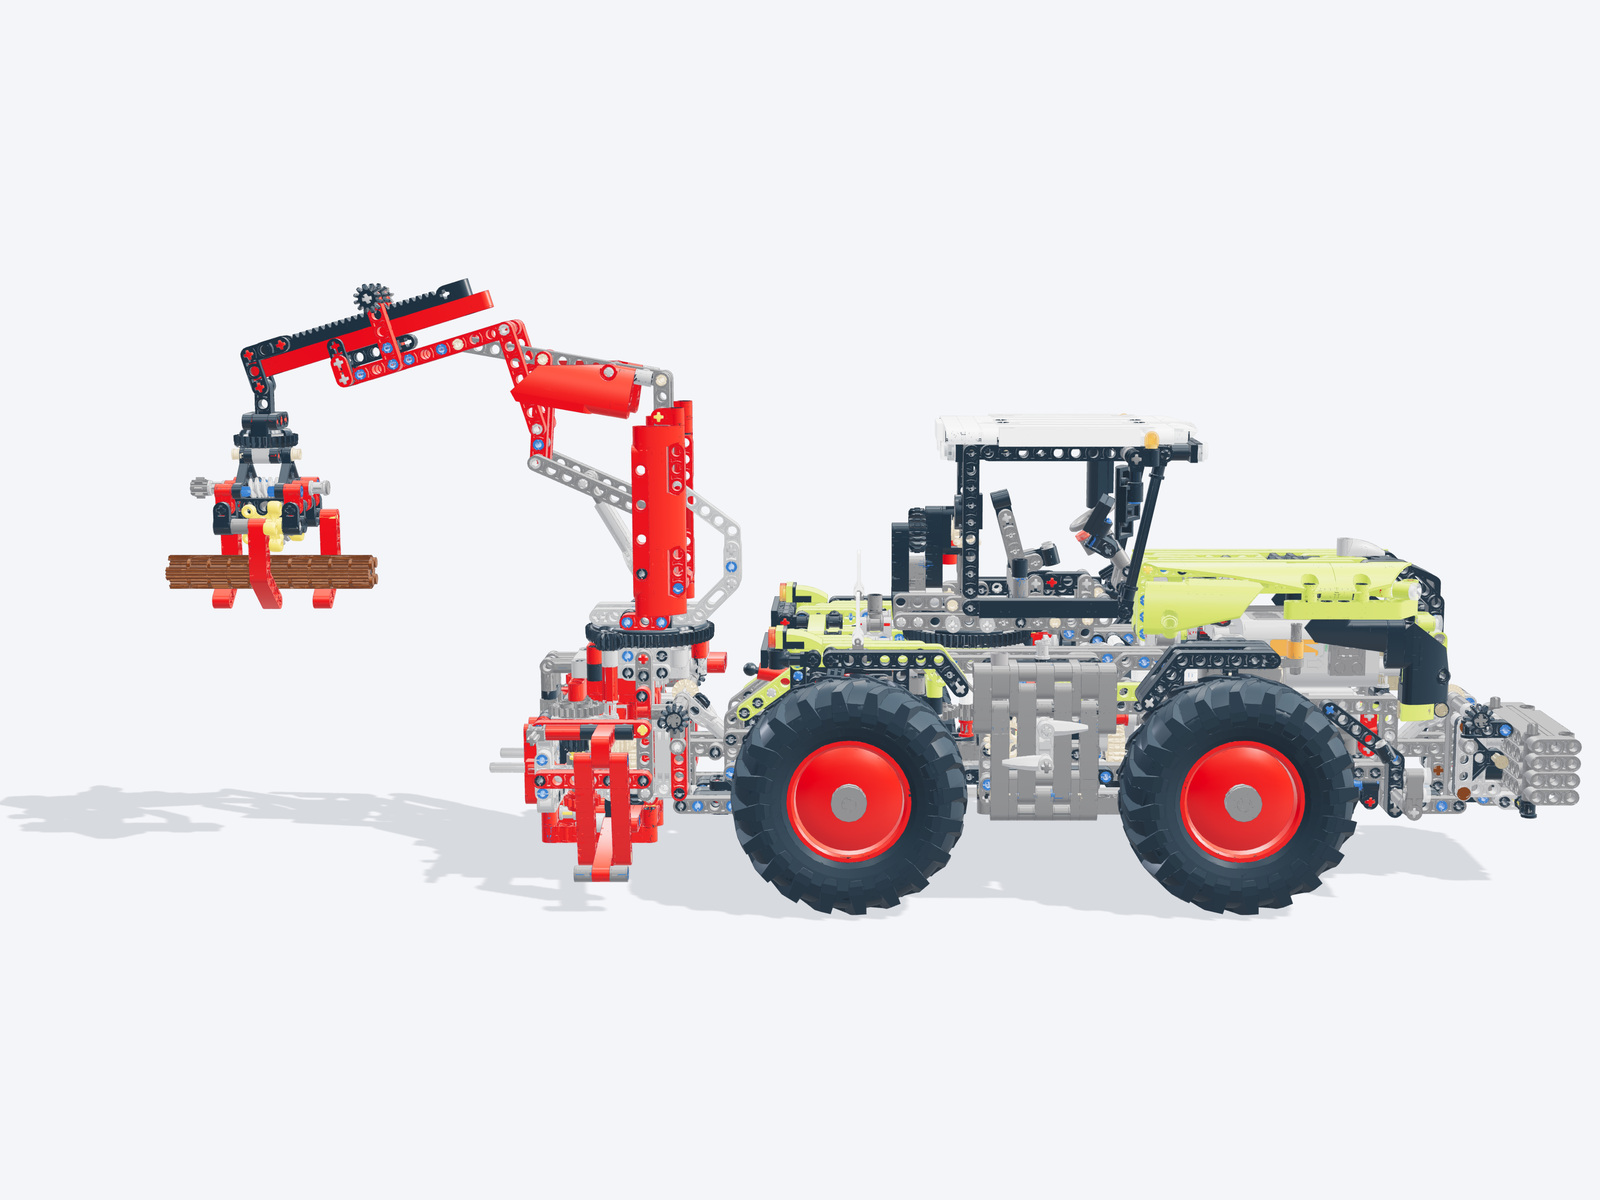
\includegraphics[width=.48\linewidth]{figures/ldraw/print/omr-42054-front.jpg}\\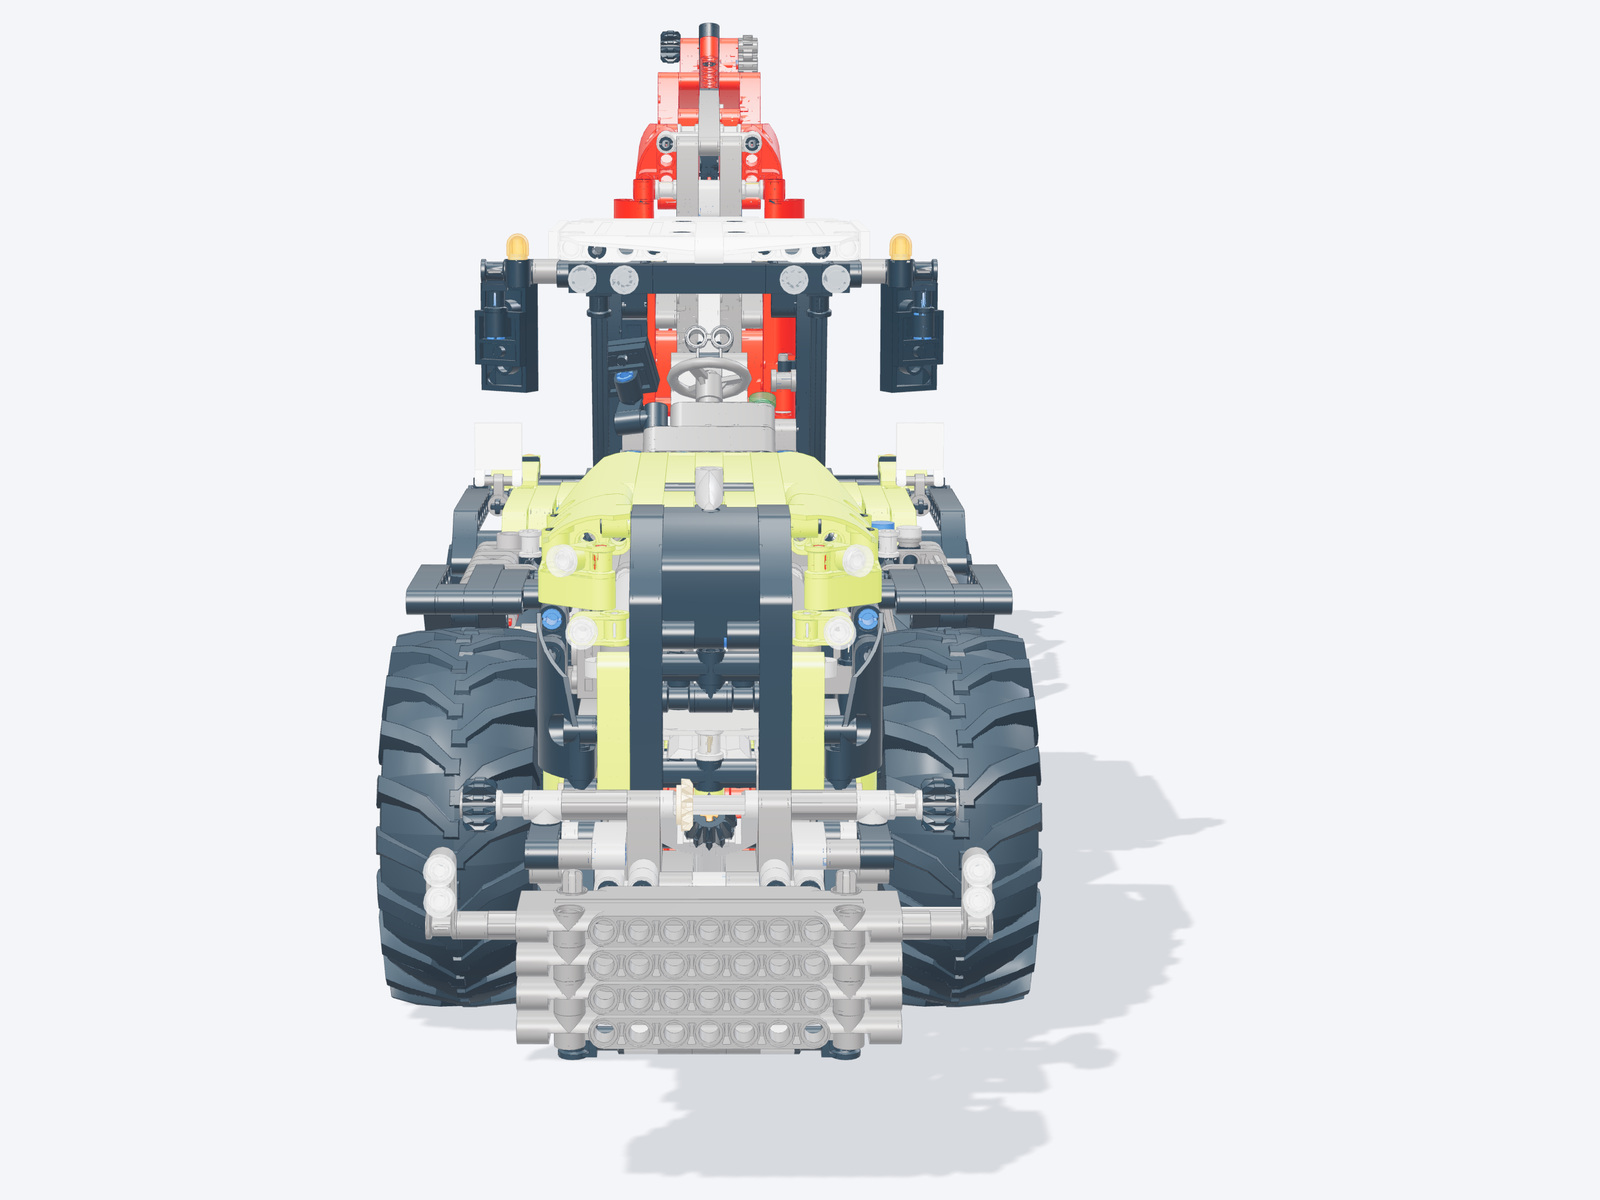
\includegraphics[width=.48\linewidth]{figures/ldraw/print/omr-42054-side.jpg}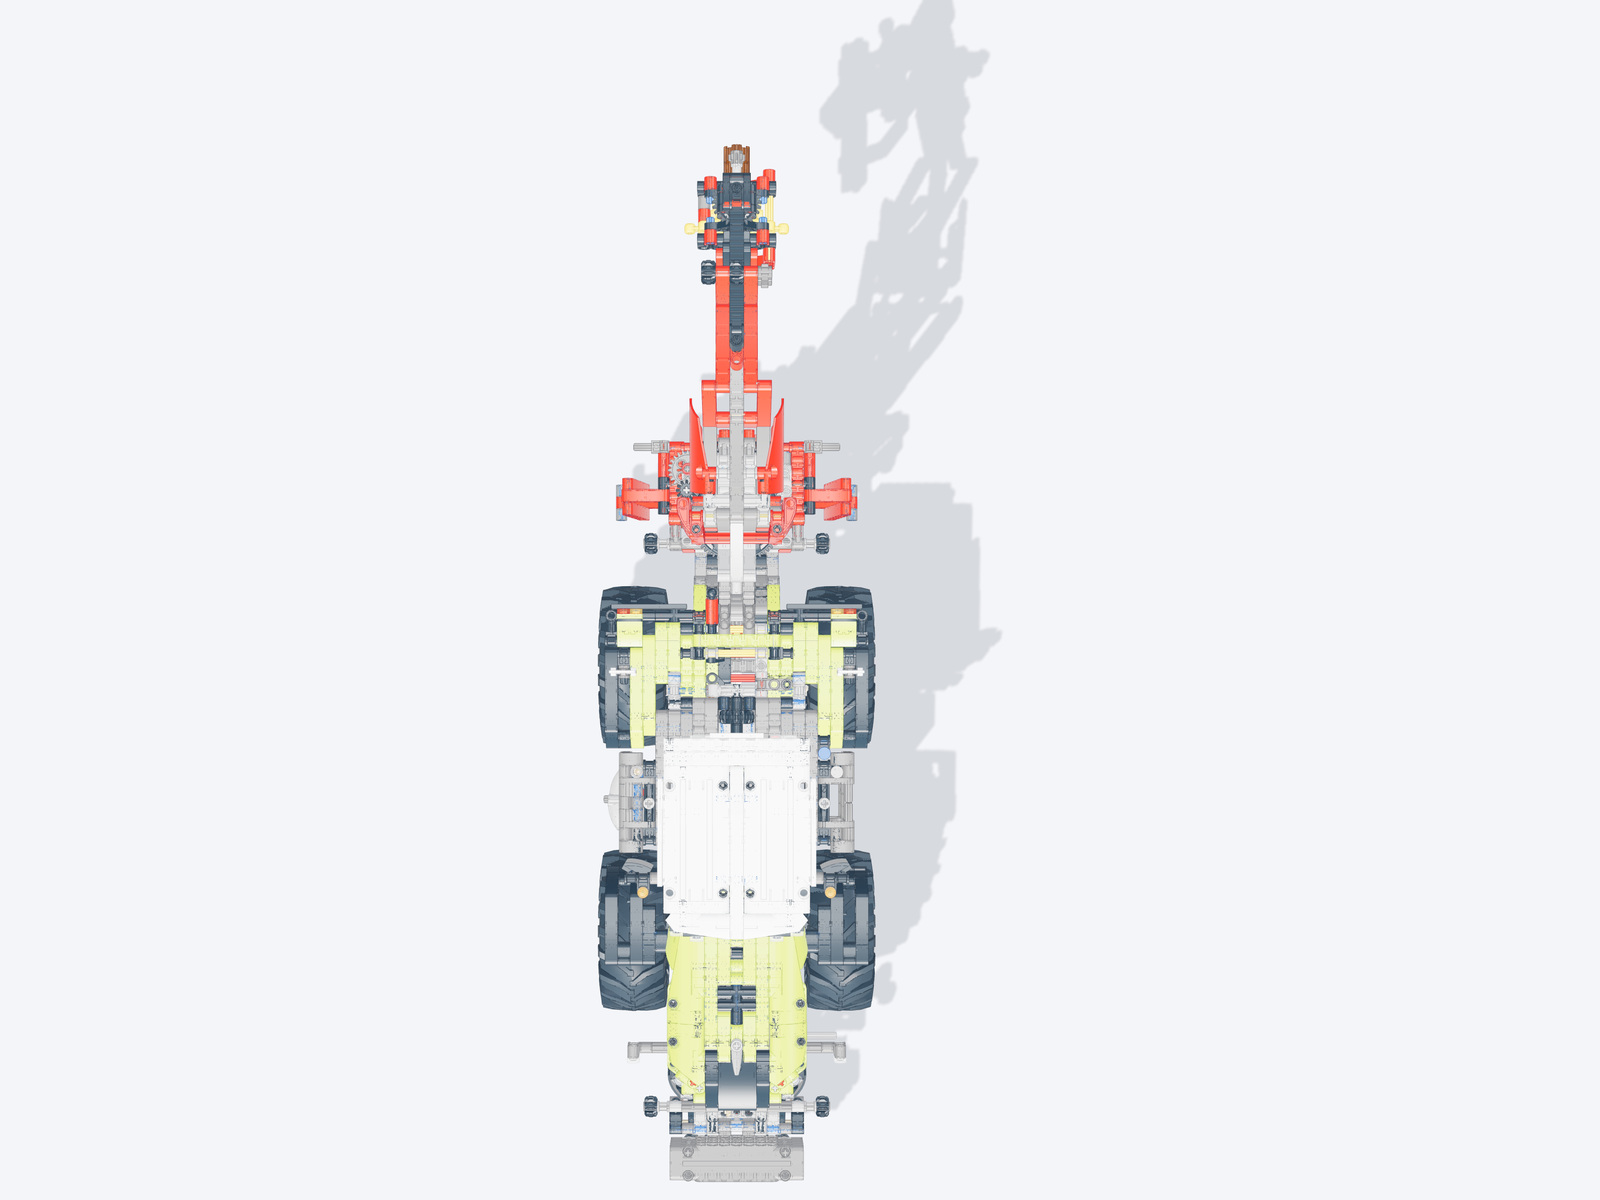
\includegraphics[width=.48\linewidth]{figures/ldraw/print/omr-42054-top.jpg}\end{center}
\paragraph{Attribution.}Philippe Hurbain [Philo]. CC BY 2.0.\par\noindent\url{https://library.ldraw.org/library/omr/42054-1.mpd}
\paragraph{Source lock.}\small\texttt{aa2856b77726aaaa74145ba1e40dbd89}\\\texttt{d1897ff3577ac2eab83237bd6d65b04c}\normalsize
\paragraph{Evidence coverage.}Connector definitions cover 98.58\% of instances. The audit reports 39 recognized-graph components and 54 intersection candidates without a recognized mating pair. 28 instances have no connector definition. These counts do not certify physical defects or gravitational stability.
\paragraph{Instructions.}229 expanded author steps.
\clearpage\subsection{Numbered visual input and complete question index}
Only relevant numbers are shown. The website can isolate any instance; public visual tasks provide their own numbered images. The following entries give every English prompt, all choice options, compact public evidence and the reference output. Raw repeated connector records and full action fact sets remain in the versioned JSON.
\begin{center}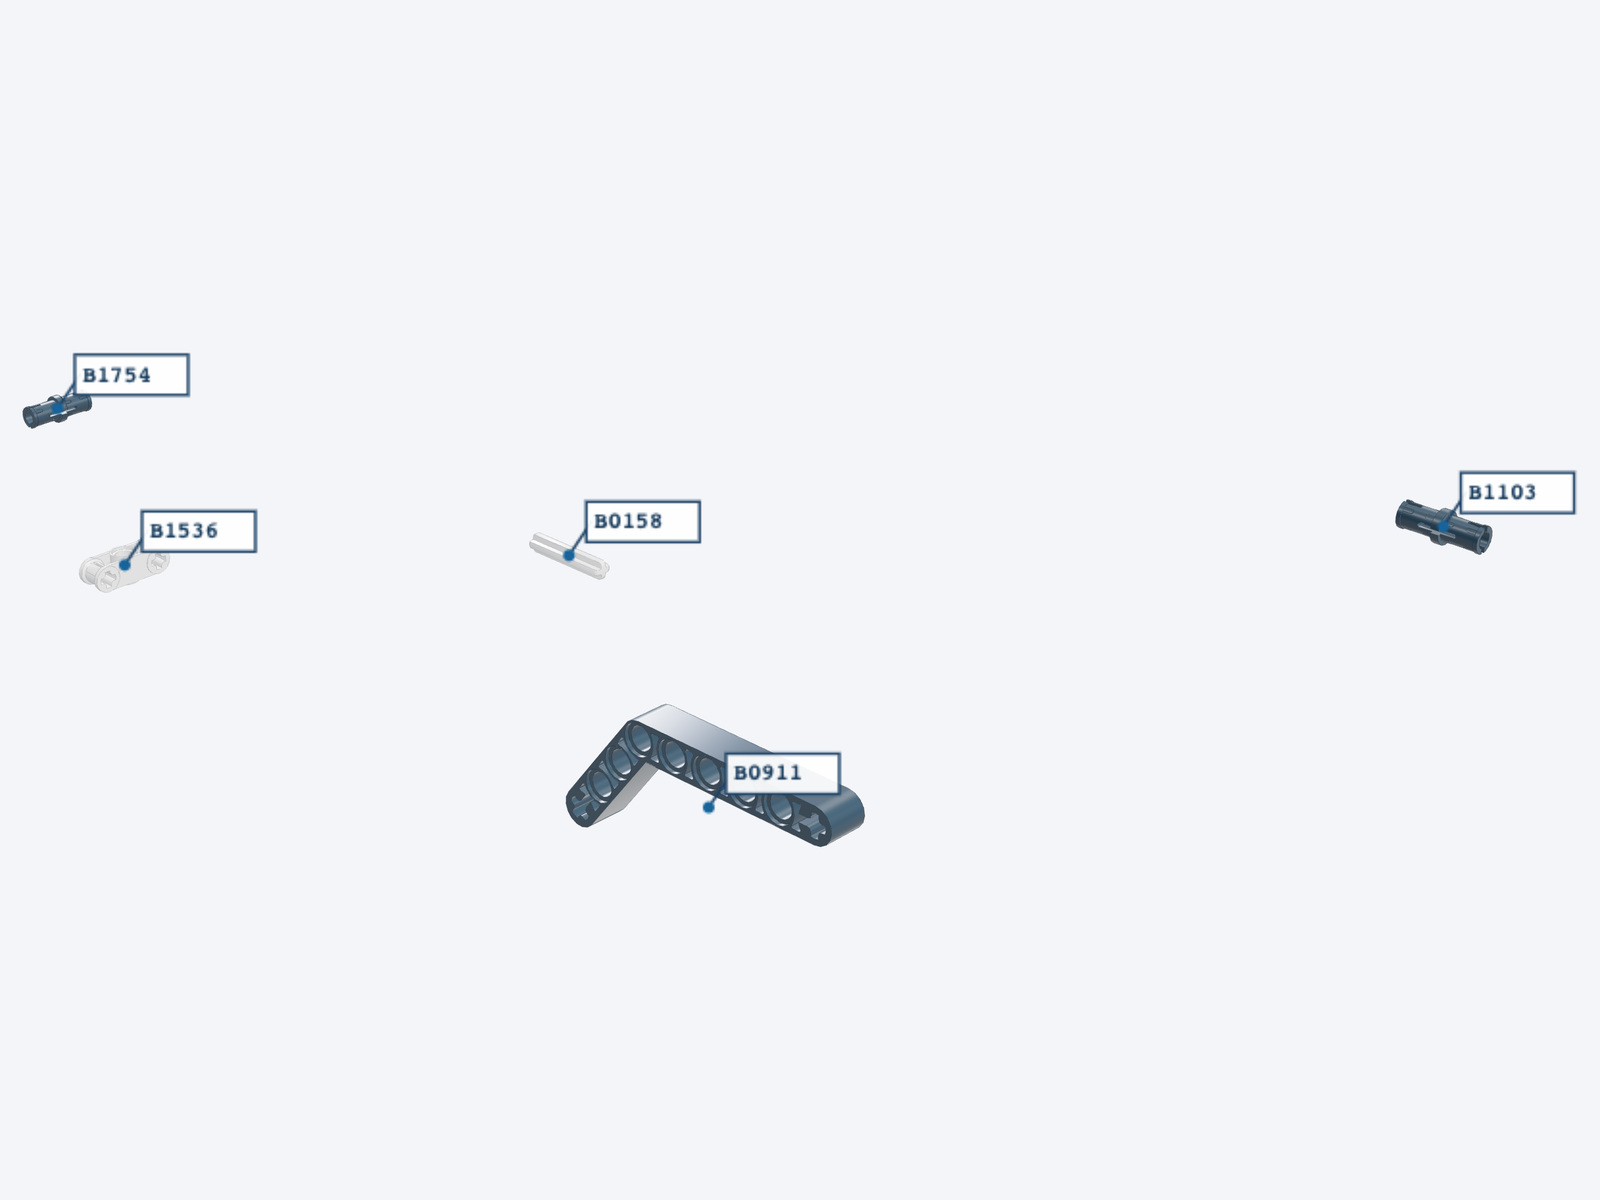
\includegraphics[width=.55\linewidth]{figures/ldraw/print/omr-42054-numbered.jpg}\end{center}
\begin{enumerate}
\item \textbf{color-1}. Identify the original color of B1103; numbered isolation is allowed.\par {\small \textit{Input:} Numbered visual input; source attributes are withheld from the model. \par\textit{Options:} A: Orange; B: Black; C: Light Bluish Grey; D: Rubber Black. \par\textit{Reference output:} B.}
\item \textbf{shape-match-1}. Ignoring color and pose, which numbered instance has the same LDraw part type as B1103?\par {\small \textit{Input:} Numbered visual input; source attributes are withheld from the model. \par\textit{Options:} A: B1754; B: B1536; C: B0158; D: B0911. \par\textit{Reference output:} A.}
\item \textbf{distance-1}. Using the supplied geometry bounding-box centers, which candidate is nearest to B1103?\par {\small \textit{Input:} Centers (mm): B1103 = (40, 144, 144); B1535 = (8, 32, -216); B0468 = (-32, 48, 106); B0455 = (-20, 68, 88). \par\textit{Options:} A: B1535; B: B0455; C: B0468. \par\textit{Reference output:} B.}
\item \textbf{color-2}. Identify the original color of B1016; numbered isolation is allowed.\par {\small \textit{Input:} Numbered visual input; source attributes are withheld from the model. \par\textit{Options:} A: Pearl Silver; B: Orange; C: Black; D: Red. \par\textit{Reference output:} C.}
\item \textbf{shape-match-2}. Ignoring color and pose, which numbered instance has the same LDraw part type as B1016?\par {\small \textit{Input:} Numbered visual input; source attributes are withheld from the model. \par\textit{Options:} A: B0191; B: B1357; C: B1766; D: B0439. \par\textit{Reference output:} D.}
\item \textbf{distance-2}. Using the supplied geometry bounding-box centers, which candidate is nearest to B1016?\par {\small \textit{Input:} Centers (mm): B1016 = (8, 120, 72); B1325 = (0, 132, -40); B1356 = (24, 128, -32); B0125 = (0, 88, -104). \par\textit{Options:} A: B0125; B: B1325; C: B1356. \par\textit{Reference output:} C.}
\item \textbf{color-3}. Identify the original color of B0570; numbered isolation is allowed.\par {\small \textit{Input:} Numbered visual input; source attributes are withheld from the model. \par\textit{Options:} A: Dark Bluish Grey; B: Trans Red; C: Trans Orange; D: Rubber Black. \par\textit{Reference output:} A.}
\item \textbf{shape-match-3}. Ignoring color and pose, which numbered instance has the same LDraw part type as B0570?\par {\small \textit{Input:} Numbered visual input; source attributes are withheld from the model. \par\textit{Options:} A: B1885; B: B1867; C: B1394; D: B0803. \par\textit{Reference output:} C.}
\item \textbf{distance-3}. Using the supplied geometry bounding-box centers, which candidate is nearest to B0570?\par {\small \textit{Input:} Centers (mm): B0570 = (16.1, 88, 176); B1586 = (0, 62, -208); B0016 = (0, 96, -24); B1159 = (30.6176, 132.6864, 73.3612). \par\textit{Options:} A: B0016; B: B1586; C: B1159. \par\textit{Reference output:} C.}
\item \textbf{color-4}. Identify the original color of B0724; numbered isolation is allowed.\par {\small \textit{Input:} Numbered visual input; source attributes are withheld from the model. \par\textit{Options:} A: White; B: Black; C: Blue; D: Pearl Silver. \par\textit{Reference output:} B.}
\item \textbf{shape-match-4}. Ignoring color and pose, which numbered instance has the same LDraw part type as B0724?\par {\small \textit{Input:} Numbered visual input; source attributes are withheld from the model. \par\textit{Options:} A: B0485; B: B0349; C: B1765; D: B0529. \par\textit{Reference output:} D.}
\item \textbf{distance-4}. Using the supplied geometry bounding-box centers, which candidate is nearest to B0724?\par {\small \textit{Input:} Centers (mm): B0724 = (-24, 100, 72); B0771 = (-40, 112, -12); B1307 = (-24, 128, -32); B0366 = (0, 86, 8). \par\textit{Options:} A: B1307; B: B0771; C: B0366. \par\textit{Reference output:} C.}
\item \textbf{color-5}. Identify the original color of B1396; numbered isolation is allowed.\par {\small \textit{Input:} Numbered visual input; source attributes are withheld from the model. \par\textit{Options:} A: Tan; B: Dark Tan; C: Dark Bluish Grey; D: Orange. \par\textit{Reference output:} C.}
\item \textbf{shape-match-5}. Ignoring color and pose, which numbered instance has the same LDraw part type as B1396?\par {\small \textit{Input:} Numbered visual input; source attributes are withheld from the model. \par\textit{Options:} A: B1763; B: B0492; C: B0793; D: B1082. \par\textit{Reference output:} D.}
\item \textbf{distance-5}. Using the supplied geometry bounding-box centers, which candidate is nearest to B1396?\par {\small \textit{Input:} Centers (mm): B1396 = (-0.1, 154.0704, 7.7276); B0365 = (0, 74, 8); B0827 = (68, 100, -20); B0049 = (16, 40, -128). \par\textit{Options:} A: B0049; B: B0365; C: B0827. \par\textit{Reference output:} B.}
\item \textbf{interface-1}. Classify the supplied connector record for B1852 and B1848. This does not certify load capacity.\par {\small \textit{Input:} Record: family = axle; connector indices = 0, 0. \par\textit{Options:} A: ball; B: axle; C: hinge; D: fixed. \par\textit{Reference output:} B.}
\item \textbf{interface-2}. Classify the supplied connector record for B1825 and B1824. This does not certify load capacity.\par {\small \textit{Input:} Record: family = hinge; connector indices = 1, 1. \par\textit{Options:} A: fixed; B: ball; C: axle; D: hinge. \par\textit{Reference output:} D.}
\item \textbf{interface-3}. Classify the supplied connector record for B0940 and B0942. This does not certify load capacity.\par {\small \textit{Input:} Record: family = stud; connector indices = 5, 0. \par\textit{Options:} A: ball; B: fixed; C: hinge; D: stud; E: axle. \par\textit{Reference output:} D.}
\item \textbf{neighbors-1}. Select every candidate directly adjacent to B1563 in the supplied connector graph.\par {\small \textit{Input:} Unique undirected pairs: B1559 / B1563; B1563 / B1565. \par\textit{Options:} A: B1565; B: B1037; C: B0192; D: B1559. \par\textit{Reference output:} A, D.}
\item \textbf{graph-removal-1}. Delete B1563 and its incident edges from this local graph. How many connected components remain? Do not infer physical extractability.\par {\small \textit{Input:} Nodes: B1563, B1559, B1565, B0192, B1037. Unique undirected pairs: B1559 / B1563; B1563 / B1565. \par\textit{Options:} A: 5; B: 3; C: 6; D: 4. \par\textit{Reference output:} D.}
\item \textbf{neighbors-2}. Select every candidate directly adjacent to B0710 in the supplied connector graph.\par {\small \textit{Input:} Unique undirected pairs: B0644 / B0710; B0710 / B0711. \par\textit{Options:} A: B1207; B: B0711; C: B1619; D: B0644. \par\textit{Reference output:} B, D.}
\item \textbf{graph-removal-2}. Delete B0710 and its incident edges from this local graph. How many connected components remain? Do not infer physical extractability.\par {\small \textit{Input:} Nodes: B0710, B0644, B0711, B1619, B1207. Unique undirected pairs: B0644 / B0710; B0710 / B0711. \par\textit{Options:} A: 3; B: 5; C: 4; D: 6. \par\textit{Reference output:} C.}
\item \textbf{neighbors-3}. Select every candidate directly adjacent to B1218 in the supplied connector graph.\par {\small \textit{Input:} Unique undirected pairs: B1216 / B1218; B1217 / B1218; B1218 / B1219. \par\textit{Options:} A: B1216; B: B0876; C: B1219; D: B1217; E: B0027. \par\textit{Reference output:} A, C, D.}
\item \textbf{graph-removal-3}. Delete B1218 and its incident edges from this local graph. How many connected components remain? Do not infer physical extractability.\par {\small \textit{Input:} Nodes: B1218, B1219, B1216, B1217, B0876, B0027. Unique undirected pairs: B1216 / B1218; B1217 / B1218; B1218 / B1219. \par\textit{Options:} A: 6; B: 5; C: 7; D: 4. \par\textit{Reference output:} B.}
\item \textbf{neighbors-4}. Select every candidate directly adjacent to B0478 in the supplied connector graph.\par {\small \textit{Input:} Unique undirected pairs: B0459 / B0478; B0462 / B0478; B0463 / B0478; B0468 / B0478; B0469 / B0478; B0478 / B0505. \par\textit{Options:} A: B0462; B: B0469; C: B0459; D: B0468; E: B0125; F: B0505; G: B0463; H: B1616. \par\textit{Reference output:} A, B, C, D, F, G.}
\item \textbf{graph-removal-4}. Delete B0478 and its incident edges from this local graph. How many connected components remain? Do not infer physical extractability.\par {\small \textit{Input:} Nodes: B0478, B0459, B0462, B0463, B0468, B0469, B0505, B1616, B0125. Unique undirected pairs: B0459 / B0478; B0462 / B0478; B0463 / B0478; B0468 / B0478; B0469 / B0478; B0478 / B0505. \par\textit{Options:} A: 8; B: 10; C: 9; D: 7. \par\textit{Reference output:} A.}
\item \textbf{neighbors-5}. Select every candidate directly adjacent to B1973 in the supplied connector graph.\par {\small \textit{Input:} Unique undirected pairs: B1967 / B1972; B1967 / B1973; B1967 / B1974; B1972 / B1973; B1973 / B1974. \par\textit{Options:} A: B1547; B: B1972; C: B1967; D: B0748; E: B1974. \par\textit{Reference output:} B, C, E.}
\item \textbf{graph-removal-5}. Delete B1973 and its incident edges from this local graph. How many connected components remain? Do not infer physical extractability.\par {\small \textit{Input:} Nodes: B1973, B1974, B1972, B1967, B1547, B0748. Unique undirected pairs: B1967 / B1972; B1967 / B1973; B1967 / B1974; B1972 / B1973; B1973 / B1974. \par\textit{Options:} A: 3; B: 2; C: 4; D: 5. \par\textit{Reference output:} A.}
\item \textbf{coverage-1}. Which numbered instance lacks a connector definition in the coverage record, so this audit cannot establish that it is floating?\par {\small \textit{Input:} Definition coverage: B0146 = unsupported; B1103 = supported; B1016 = supported; B0570 = supported. \par\textit{Options:} A: B1103; B: B0146; C: B0570; D: B1016. \par\textit{Reference output:} B.}
\item \textbf{evidence-limit-1}. Only source geometry, connector matching and mesh intersection audits are available. Without mass, friction, material or dynamic tests, is gravitational stability established?\par {\small \textit{Input:} Available evidence: Original CAD; Connector inference; Inset-mesh intersection candidates. \par\textit{Options:} A: Not established by this evidence; B: Established. \par\textit{Reference output:} A.}
\item \textbf{source-step-1}. At which expanded author step does B1230 first appear in the supplied source-step table? Source order is not a collision-free assembly proof.\par {\small \textit{Input:} Expanded author records: step 1: B0001; step 135: B1230. \par\textit{Options:} A: 136; B: 134; C: 137; D: 135. \par\textit{Reference output:} D.}
\item \textbf{source-step-2}. At which expanded author step does B1177 first appear in the supplied source-step table? Source order is not a collision-free assembly proof.\par {\small \textit{Input:} Expanded author records: step 1: B0001; step 131: B1177. \par\textit{Options:} A: 133; B: 131; C: 132; D: 130. \par\textit{Reference output:} B.}
\item \textbf{source-step-3}. At which expanded author step does B0711 first appear in the supplied source-step table? Source order is not a collision-free assembly proof.\par {\small \textit{Input:} Expanded author records: step 1: B0001; step 85: B0711. \par\textit{Options:} A: 84; B: 87; C: 86; D: 85. \par\textit{Reference output:} D.}
\item \textbf{source-step-4}. At which expanded author step does B0180 first appear in the supplied source-step table? Source order is not a collision-free assembly proof.\par {\small \textit{Input:} Expanded author records: step 1: B0001; step 19: B0180. \par\textit{Options:} A: 20; B: 18; C: 21; D: 19. \par\textit{Reference output:} D.}
\item \textbf{source-step-5}. At which expanded author step does B0363 first appear in the supplied source-step table? Source order is not a collision-free assembly proof.\par {\small \textit{Input:} Expanded author records: step 1: B0001; step 43: B0363. \par\textit{Options:} A: 45; B: 42; C: 43; D: 44. \par\textit{Reference output:} C.}
\item \textbf{source-sequence-1}. Reveal the supplied source-step window in author order. Actions change visibility only, without simulating insertion trajectories.\par {\small \textit{Input:} Source window: step-1: B0001, B0002, B0003, B0004, B0005, B0006, B0007, B0008, B0009, B0010, B0011, B0012, B0013, B0014, B0015, B0016, B0017; step-2: B0018, B0019, B0020, B0021, B0022, B0023, B0024, B0025, B0026; step-3: B0027, B0028, B0029, B0030, B0031, B0032, B0033, B0034, B0035, B0036, B0037; step-4: B0038, B0039, B0040, B0041, B0042, B0043, B0044, B0045, B0046; step-5: B0047, B0048, B0049, B0050, B0051, B0052; step-6: B0053, B0054, B0055, B0056, B0057, B0058. Action budget: 6. \par\textit{Reference output:} step-1, step-2, step-3, step-4, step-5, step-6.}
\item \textbf{restore-instance-1}. The display copy hides B1103. Restore only that numbered instance, preserving all other instances and source poses.\par {\small \textit{Input:} Target: B1103. Action budget: 1. All other instances initially remain visible. \par\textit{Reference output:} restore-B1103.}
\item \textbf{restore-instance-2}. The display copy hides B1016. Restore only that numbered instance, preserving all other instances and source poses.\par {\small \textit{Input:} Target: B1016. Action budget: 1. All other instances initially remain visible. \par\textit{Reference output:} restore-B1016.}
\item \textbf{restore-instance-3}. The display copy hides B0570. Restore only that numbered instance, preserving all other instances and source poses.\par {\small \textit{Input:} Target: B0570. Action budget: 1. All other instances initially remain visible. \par\textit{Reference output:} restore-B0570.}
\end{enumerate}

\end{document}
